\section{Equalizer}\label{sec:tech_equalizer}


\begin{figure}[H]
\centering
\begin{subfigure}[t]{0.47\textwidth}
	\tikzsetnextfilename{parametric_eq_preanalysis_Q}
	% This file was created by matlab2tikz.
%
%The latest updates can be retrieved from
%  http://www.mathworks.com/matlabcentral/fileexchange/22022-matlab2tikz-matlab2tikz
%where you can also make suggestions and rate matlab2tikz.
%
\begin{tikzpicture}

\begin{axis}[%
width=2in,
height=1.7in,
at={(1.011in,0.642in)},
scale only axis,
xmode=log,
xmin=10,
xmax=20000,
xminorticks=true,
xlabel={Frequency [Hz]},
xmajorgrids,
xminorgrids,
ymin=-5,
ymax=5,
ymajorgrids,
yticklabels={\empty},
axis background/.style={fill=white}
]
\addplot [color=black,solid,line width=1.0pt,forget plot]
  table[row sep=crcr]{%
0.159154943091895	1.52104528479092e-09\\
5.67189079114852	1.93230452791098e-06\\
11.1846266392052	7.51943373818724e-06\\
16.6973624872618	1.67791992824004e-05\\
22.2100983353184	2.97386492611314e-05\\
27.722834183375	4.64357337452805e-05\\
33.2355700314317	6.6919516788473e-05\\
38.7483058794883	9.12504455800552e-05\\
44.2610417275449	0.000119500686962666\\
49.7737775756016	0.00015175453242015\\
55.2865134236582	0.000188108874101866\\
60.7992492717148	0.000228673755853626\\
66.3119851197714	0.000273573008712253\\
71.8247209678281	0.000322944971695505\\
77.3374568158847	0.000376943308720189\\
82.8501926639413	0.000435737928385534\\
88.362928511998	0.000499516015079531\\
93.8756643600546	0.000568483184814175\\
99.3884002081112	0.000642864774463703\\
104.901136056168	0.000722907281943459\\
110.413871904224	0.000808879967186518\\
115.926607752281	0.00090107664260089\\
121.439343600338	0.000999817659988643\\
126.952079448394	0.00110545212673103\\
132.464815296451	0.00121836037701581\\
137.977551144508	0.00133895672322284\\
143.490286992564	0.0014676925275577\\
149.003022840621	0.00160505963325159\\
154.515758688678	0.00175159419615416\\
160.028494536734	0.00190788097717544\\
165.541230384791	0.00207455814919004\\
171.053966232847	0.00225232269285828\\
176.566702080904	0.00244193645895823\\
182.079437928961	0.00264423299601844\\
187.592173777017	0.00286012524226615\\
193.104909625074	0.00309061422509228\\
198.617645473131	0.00333679889352346\\
204.130381321187	0.0035998872811627\\
209.643117169244	0.00388120918199709\\
215.1558530173	0.00418223059313337\\
220.668588865357	0.00450457019596922\\
226.181324713414	0.00485001821500331\\
231.69406056147	0.00522055805142346\\
237.206796409527	0.00561839115630346\\
242.719532257584	0.00604596571734974\\
248.23226810564	0.00650600982730972\\
253.745003953697	0.00700156994994694\\
259.257739801753	0.0075360556701881\\
264.77047564981	0.00811329191767284\\
270.283211497867	0.00873758011500236\\
275.795947345923	0.00941377003543197\\
281.30868319398	0.0101473445408142\\
286.821419042037	0.0109445199075512\\
292.334154890093	0.0118123650807287\\
297.84689073815	0.0127589440154928\\
303.359626586207	0.0137934863589725\\
308.872362434263	0.0149265930350138\\
314.38509828232	0.0161704851220586\\
319.897834130376	0.0175393066793845\\
325.410569978433	0.0190494952573068\\
330.92330582649	0.0207202378147141\\
336.436041674546	0.0225740352218158\\
341.948777522603	0.0246374057041767\\
347.46151337066	0.026941767528892\\
352.974249218716	0.0295245547390489\\
358.486985066773	0.0324306385239295\\
363.999720914829	0.0357141531425909\\
369.512456762886	0.039440862570496\\
375.025192610943	0.0436912575325603\\
380.537928458999	0.048564650265103\\
386.050664307056	0.054184648799545\\
391.563400155113	0.0607065637125135\\
397.076136003169	0.0683275602848587\\
402.588871851226	0.077300770911441\\
408.101607699282	0.0879552153580892\\
413.614343547339	0.100724392830506\\
419.127079395396	0.116188077803\\
424.639815243452	0.135134653259035\\
430.152551091509	0.158656139597021\\
435.665286939566	0.188296609753382\\
441.178022787622	0.226290199861444\\
446.690758635679	0.275953977089983\\
452.203494483736	0.342356864070059\\
457.716230331792	0.433496108720002\\
463.228966179849	0.562432570648061\\
468.741702027905	0.751262614355034\\
474.254437875962	1.03851439355349\\
479.767173724019	1.49189799388277\\
485.279909572075	2.22208716337385\\
490.792645420132	3.34311701685435\\
496.305381268189	4.6247041751038\\
501.818117116245	4.90410608874762\\
507.330852964302	3.82505415494008\\
512.843588812358	2.61985771101294\\
518.356324660415	1.78382846965615\\
523.869060508472	1.25552325827228\\
529.381796356528	0.919021771091239\\
534.894532204585	0.697266219629312\\
540.407268052642	0.545468778132612\\
545.920003900698	0.437813601428799\\
551.432739748755	0.359040714427765\\
556.945475596812	0.299818721083128\\
562.458211444868	0.254241272727278\\
567.970947292925	0.218447077317677\\
573.483683140981	0.189836549255888\\
578.996418989038	0.16661277724288\\
584.509154837095	0.147504053855288\\
590.021890685151	0.131591195560257\\
595.534626533208	0.11819715359357\\
601.047362381265	0.106814691905798\\
606.560098229321	0.0970579326173343\\
612.072834077378	0.0886292233685626\\
617.585569925434	0.0812960559803955\\
623.098305773491	0.0748747112899249\\
628.611041621548	0.0692184879859231\\
634.123777469604	0.0642091084514587\\
639.636513317661	0.059750360839324\\
645.149249165718	0.0557633378864817\\
650.661985013774	0.0521828310419649\\
656.174720861831	0.0489545708600188\\
661.687456709888	0.046033094400842\\
667.200192557944	0.0433800821776765\\
672.712928406001	0.0409630502277672\\
678.225664254057	0.0387543132948973\\
683.738400102114	0.0367301567900939\\
689.251135950171	0.0348701708602796\\
694.763871798227	0.0331567112872759\\
700.276607646284	0.0315744603585919\\
705.789343494341	0.0301100670650826\\
711.302079342397	0.0287518506571268\\
716.814815190454	0.0274895551298186\\
722.32755103851	0.0263141448589172\\
727.840286886567	0.0252176336998925\\
733.353022734624	0.0241929414171724\\
738.86575858268	0.0232337725625455\\
744.378494430737	0.0223345138732211\\
749.891230278794	0.0214901470217593\\
755.40396612685	0.0206961741416183\\
760.916701974907	0.0199485540338976\\
766.429437822963	0.0192436473393069\\
771.94217367102	0.0185781692575445\\
777.454909519077	0.0179491486526881\\
782.967645367133	0.017353892572703\\
788.48038121519	0.0167899553784511\\
793.993117063246	0.0162551118115383\\
799.505852911303	0.0157473334318375\\
805.01858875936	0.0152647679548883\\
810.531324607416	0.0148057210832129\\
816.044060455473	0.0143686404969937\\
821.55679630353	0.0139521017104333\\
827.069532151586	0.0135547955551384\\
832.582267999643	0.0131755170712662\\
838.0950038477	0.012813155636846\\
843.607739695756	0.01246668617149\\
849.120475543813	0.0121351612900779\\
854.633211391869	0.0118177042848058\\
860.145947239926	0.0115135028395057\\
865.658683087983	0.011221803389484\\
871.171418936039	0.0109419060530408\\
876.684154784096	0.0106731600667184\\
882.196890632153	0.0104149596707135\\
887.709626480209	0.010166740392277\\
893.222362328266	0.00992797568316446\\
898.735098176323	0.00969817387615866\\
904.247834024379	0.00947687542142251\\
909.760569872436	0.00926365037957695\\
915.273305720492	0.00905809613688407\\
920.786041568549	0.00885983533102005\\
926.298777416606	0.00866851395226085\\
931.811513264662	0.00848379961467099\\
937.324249112719	0.00830537997469444\\
942.836984960776	0.00813296128321451\\
948.349720808832	0.00796626705919894\\
953.862456656889	0.00780503687267413\\
959.375192504945	0.00764902522840434\\
964.887928353002	0.00749800053779741\\
970.400664201059	0.00735174417577524\\
975.913400049115	0.00721004960777091\\
981.426135897172	0.00707272158928544\\
986.938871745229	0.00693957542511233\\
992.451607593285	0.00681043628269342\\
997.964343441342	0.00668513856262366\\
1003.4770792894	0.0065635253112589\\
1008.98981513746	0.00644544767835877\\
1014.50255098551	0.00633076441469318\\
1020.01528683357	0.00621934140630503\\
1025.52802268163	0.00611105123922509\\
1031.04075852968	0.00600577279878325\\
1036.55349437774	0.00590339089400462\\
1042.06623022579	0.00580379590976603\\
1047.57896607385	0.00570688348170515\\
1053.09170192191	0.0056125541930468\\
1058.60443776996	0.00552071329318637\\
1064.11717361802	0.00543127043321141\\
1069.62990946608	0.00534413942012012\\
1075.14264531413	0.0052592379865762\\
1080.65538116219	0.00517648757571804\\
1086.16811701025	0.00509581313833509\\
1091.6808528583	0.00501714294610182\\
1097.19358870636	0.00494040841231004\\
1102.70632455442	0.00486554392802055\\
1108.21906040247	0.00479248670487366\\
1113.73179625053	0.00472117662911945\\
1119.24453209859	0.00465155612450848\\
1124.75726794664	0.00458357002297077\\
1130.2700037947	0.00451716544255485\\
1135.78273964276	0.0044522916741971\\
1141.29547549081	0.00438890007307048\\
1146.80821133887	0.0043269439571779\\
1152.32094718693	0.00426637851274\\
1157.83368303498	0.00420716070243075\\
1163.34641888304	0.00414924918155447\\
1168.8591547311	0.00409260421693544\\
1174.37189057915	0.00403718761152211\\
1179.88462642721	0.00398296263238773\\
1185.39736227527	0.00392989394260601\\
1190.91009812332	0.00387794753818219\\
1196.42283397138	0.00382709068586065\\
1201.93556981944	0.00377729186687577\\
1207.44830566749	0.0037285207220526\\
1212.96104151555	0.00368074799995988\\
1218.47377736361	0.00363394550881578\\
1223.98651321166	0.00358808606891927\\
1229.49924905972	0.00354314346991455\\
1235.01198490778	0.00349909242784334\\
1240.52472075583	0.0034559085468669\\
1246.03745660389	0.00341356827984536\\
1251.55019245195	0.00337204889433326\\
1257.0629283	0.00333132843704734\\
1262.57566414806	0.00329138570244961\\
1268.08839999612	0.00325220020158058\\
1273.60113584417	0.00321375213273901\\
1279.11387169223	0.00317602235370764\\
1284.62660754029	0.00313899235481557\\
1290.13934338834	0.00310264423424481\\
1295.6520792364	0.00306696067302852\\
1301.16481508446	0.00303192491288174\\
1306.67755093251	0.00299752073380497\\
1312.19028678057	0.00296373243322678\\
1317.70302262863	0.00293054480564248\\
1323.21575847668	0.00289794312435304\\
1328.72849432474	0.00286591312222918\\
1334.2412301728	0.00283444097538565\\
1339.75396602085	0.00280351328552027\\
1345.26670186891	0.00277311706438818\\
1350.77943771697	0.0027432397188826\\
1356.29217356502	0.00271386903623614\\
1361.80490941308	0.00268499316985941\\
1367.31764526114	0.00265660062629918\\
1372.83038110919	0.00262868025278185\\
1378.34311695725	0.00260122122404099\\
1383.85585280531	0.00257421303140194\\
1389.36858865336	0.00254764547186784\\
1394.88132450142	0.002521508636239\\
1400.39406034948	0.00249579289956674\\
1405.90679619753	0.00247048891134444\\
1411.41953204559	0.00244558758573287\\
1416.93226789365	0.002421080092645\\
1422.4450037417	0.00239695784848904\\
1427.95773958976	0.0023732125088894\\
1433.47047543782	0.00234983595947141\\
1438.98321128587	0.00232682030881676\\
1444.49594713393	0.00230415788105415\\
1450.00868298199	0.00228184120821058\\
1455.52141883004	0.00225986302389273\\
1461.0341546781	0.00223821625641463\\
1466.54689052616	0.0022168940224824\\
1472.05962637421	0.00219588962126232\\
1477.57236222227	0.00217519652836194\\
1483.08509807033	0.00215480839014459\\
1488.59783391838	0.00213471901847157\\
1494.11056976644	0.00211492238540767\\
1499.6233056145	0.00209541261804977\\
1505.13604146255	0.00207618399386629\\
1510.64877731061	0.00205723093592845\\
1516.16151315867	0.00203854800845373\\
1521.67424900672	0.0020201299122875\\
1527.18698485478	0.00200197148114609\\
1532.69972070283	0.00198406767705373\\
1538.21245655089	0.00196641358702312\\
1543.72519239895	0.00194900441871381\\
1549.237928247	0.00193183549725902\\
1554.75066409506	0.00191490226155436\\
1560.26339994312	0.0018982002610304\\
1565.77613579117	0.00188172515230368\\
1571.28887163923	0.00186547269607827\\
1576.80160748729	0.00184943875403952\\
1582.31434333534	0.00183361928609289\\
1587.8270791834	0.00181801034732114\\
1593.33981503146	0.00180260808546209\\
1598.85255087951	0.00178740873816454\\
1604.36528672757	0.00177240863039448\\
1609.87802257563	0.001757604172092\\
1615.39075842368	0.0017429918557586\\
1620.90349427174	0.00172856825387864\\
1626.4162301198	0.00171433001722007\\
1631.92896596785	0.00170027387209956\\
1637.44170181591	0.00168639661886817\\
1642.95443766397	0.00167269512947912\\
1648.46717351202	0.00165916634550482\\
1653.97990936008	0.00164580727659151\\
1659.49264520814	0.00163261499832965\\
1665.00538105619	0.00161958665072776\\
1670.51811690425	0.00160671943604798\\
1676.03085275231	0.00159401061778507\\
1681.54358860036	0.00158145751853466\\
1687.05632444842	0.00156905751874846\\
1692.56906029648	0.00155680805479339\\
1698.08179614453	0.00154470661814053\\
1703.59453199259	0.00153275075328537\\
1709.10726784065	0.00152093805680557\\
1714.6200036887	0.00150926617602739\\
1720.13273953676	0.00149773280721376\\
1725.64547538482	0.00148633569507711\\
1731.15821123287	0.00147507263093657\\
1736.67094708093	0.00146394145175835\\
1742.18368292899	0.0014529400391497\\
1747.69641877704	0.00144206631798664\\
1753.2091546251	0.0014313182555139\\
1758.72189047316	0.0014206938603062\\
1764.23462632121	0.00141019118091697\\
1769.74736216927	0.00139980830552986\\
1775.26009801733	0.00138954336033172\\
1780.77283386538	0.00137939450905026\\
1786.28556971344	0.00136935995170113\\
1791.7983055615	0.00135943792404647\\
1797.31104140955	0.00134962669652705\\
1802.82377725761	0.00133992457329465\\
1808.33651310567	0.00133032989188273\\
1813.84924895372	0.00132084102181647\\
1819.36198480178	0.00131145636443378\\
1824.87472064984	0.00130217435167278\\
1830.38745649789	0.00129299344565364\\
1835.90019234595	0.00128391213778806\\
1841.41292819401	0.00127492894817405\\
1846.92566404206	0.00126604242505828\\
1852.43839989012	0.00125725114395507\\
1857.95113573818	0.00124855370706049\\
1863.46387158623	0.00123994874293254\\
1868.97660743429	0.00123143490542309\\
1874.48934328235	0.0012230108735933\\
1880.0020791304	0.00121467535073426\\
1885.51481497846	0.00120642706401438\\
1891.02755082652	0.00119826476401676\\
1896.54028667457	0.00119018722401632\\
1902.05302252263	0.00118219323974091\\
1907.56575837069	0.00117428162845553\\
1913.07849421874	0.00116645122908594\\
1918.5912300668	0.00115870090108501\\
1924.10396591486	0.00115102952453896\\
1929.61670176291	0.00114343599935377\\
1935.12943761097	0.00113591924508374\\
1940.64217345903	0.00112847820026829\\
1946.15490930708	0.00112111182221618\\
1951.66764515514	0.00111381908650813\\
1957.1803810032	0.00110659898660938\\
1962.69311685125	0.00109945053349381\\
1968.20585269931	0.00109237275532592\\
1973.71858854737	0.00108536469706756\\
1979.23132439542	0.00107842542003069\\
1984.74406024348	0.00107155400169241\\
1990.25679609154	0.00106474953529783\\
1995.76953193959	0.00105801112946678\\
2001.28226778765	0.00105133790797996\\
2006.79500363571	0.00104472900935471\\
2012.30773948376	0.0010381835867218\\
2017.82047533182	0.0010317008072026\\
2023.33321117987	0.00102527985206159\\
2028.84594702793	0.00101891991603342\\
2034.35868287599	0.00101262020730954\\
2039.87141872404	0.00100637994701951\\
2045.3841545721	0.00100019836925045\\
2050.89689042016	0.00099407472056883\\
2056.40962626821	0.000988008259883694\\
2061.92236211627	0.000981998258161303\\
2067.43509796433	0.000976043998249759\\
2072.94783381238	0.000970144774495331\\
2078.46056966044	0.000964299892678894\\
2083.9733055085	0.000958508669655401\\
2089.48604135655	0.000952770433365526\\
2094.99877720461	0.00094708452231314\\
2100.51151305267	0.00094145028544389\\
2106.02424890072	0.000935867082253264\\
2111.53698474878	0.0009303342820905\\
2117.04972059684	0.000924851264451771\\
2122.56245644489	0.000919417418361226\\
2128.07519229295	0.000914032142413475\\
2133.58792814101	0.000908694844696523\\
2139.10066398906	0.000903404942325138\\
2144.61339983712	0.000898161861408133\\
2150.12613568518	0.000892965037038778\\
2155.63887153323	0.000887813912876385\\
2161.15160738129	0.000882707941109721\\
2166.66434322935	0.000877646582254575\\
2172.1770790774	0.000872629305047741\\
2177.68981492546	0.000867655586356437\\
2183.20255077352	0.000862724910740591\\
2188.71528662157	0.000857836770726728\\
2194.22802246963	0.000852990666287338\\
2199.74075831769	0.000848186104993265\\
2205.25349416574	0.000843422601674342\\
2210.7662300138	0.000838699678377012\\
2216.27896586186	0.000834016864229373\\
2221.79170170991	0.000829373695312013\\
2227.30443755797	0.000824769714488344\\
2232.81717340603	0.000820204471418143\\
2238.32990925408	0.000815677522204675\\
2243.84264510214	0.000811188429529727\\
2249.3553809502	0.000806736762325801\\
2254.86811679825	0.000802322095886071\\
2260.38085264631	0.000797944011534653\\
2265.89358849437	0.000793602096618917\\
2271.40632434242	0.0007892959444536\\
2276.91906019048	0.000785025154099057\\
2282.43179603854	0.00078078933042108\\
2287.94453188659	0.00077658808377658\\
2293.45726773465	0.000772421030140901\\
2298.97000358271	0.0007682877908475\\
2304.48273943076	0.00076418799255712\\
2309.99547527882	0.00076012126723082\\
2315.50821112688	0.00075608725191015\\
2321.02094697493	0.000752085588738394\\
2326.53368282299	0.000748115924777387\\
2332.04641867105	0.00074417791204611\\
2337.5591545191	0.000740271207335578\\
2343.07189036716	0.000736395472168364\\
2348.58462621522	0.000732550372709916\\
2354.09736206327	0.000728735579649006\\
2359.61009791133	0.000724950768303823\\
2365.12283375939	0.000721195618276794\\
2370.63556960744	0.000717469813593452\\
2376.1483054555	0.000713773042528897\\
2381.66104130356	0.000710104997542243\\
2387.17377715161	0.000706465375232283\\
2392.68651299967	0.000702853876327865\\
2398.19924884773	0.000699270205496988\\
2403.71198469578	0.00069571407135068\\
2409.22472054384	0.000692185186414083\\
2414.7374563919	0.000688683266962552\\
2420.25019223995	0.000685208033040952\\
2425.76292808801	0.000681759208415467\\
2431.27566393607	0.000678336520482972\\
2436.78839978412	0.000674939700141838\\
2442.30113563218	0.000671568481855594\\
2447.81387148024	0.00066822260361629\\
2453.32660732829	0.000664901806684175\\
2458.83934317635	0.000661605835757408\\
2464.35207902441	0.000658334438796587\\
2469.86481487246	0.000655087367061398\\
2475.37755072052	0.00065186437491585\\
2480.89028656857	0.000648665219972927\\
2486.40302241663	0.000645489662870896\\
2491.91575826469	0.000642337467306096\\
2497.42849411275	0.000639208400034887\\
2502.9412299608	0.000636102230692377\\
2508.45396580886	0.000633018731836788\\
2513.96670165692	0.000629957678980327\\
2519.47943750497	0.000626918850296062\\
2524.99217335303	0.000623902026876351\\
2530.50490920108	0.000620906992540003\\
2536.01764504914	0.000617933533695364\\
2541.5303808972	0.000614981439465678\\
2547.04311674525	0.000612050501664029\\
2552.55585259331	0.000609140514509856\\
2558.06858844137	0.000606251274968383\\
2563.58132428942	0.000603382582299355\\
2569.09406013748	0.00060053423834825\\
2574.60679598554	0.000597706047339941\\
2580.11953183359	0.000594897815913415\\
2585.63226768165	0.000592109353044639\\
2591.14500352971	0.000589340470008002\\
2596.65773937776	0.000586590980358963\\
2602.17047522582	0.000583860700013128\\
2607.68321107388	0.000581149446935767\\
2613.19594692193	0.000578457041384816\\
2618.70868276999	0.000575783305721886\\
2624.22141861805	0.000573128064477843\\
2629.7341544661	0.000570491144262171\\
2635.24689031416	0.000567872373691629\\
2640.75962616222	0.000565271583511748\\
2646.27236201027	0.000562688606340347\\
2651.78509785833	0.000560123276866178\\
2657.29783370639	0.000557575431725507\\
2662.81056955444	0.000555044909413405\\
2668.3233054025	0.000552531550353183\\
2673.83604125056	0.000550035196811542\\
2679.34877709861	0.000547555692929438\\
2684.86151294667	0.000545092884616012\\
2690.37424879473	0.000542646619571745\\
2695.88698464278	0.000540216747276888\\
2701.39972049084	0.000537803118968326\\
2706.9124563389	0.000535405587475657\\
2712.42519218695	0.000533024007504694\\
2717.93792803501	0.000530658235263332\\
2723.45066388307	0.000528308128662121\\
2728.96339973112	0.000525973547240987\\
2734.47613557918	0.000523654352111381\\
2739.98887142724	0.000521350405975565\\
2745.50160727529	0.000519061573093839\\
2751.01434312335	0.00051678771920161\\
2756.52707897141	0.000514528711648259\\
2762.03981481946	0.000512284419140641\\
2767.55255066752	0.000510054711984163\\
2773.06528651558	0.000507839461851364\\
2778.57802236363	0.000505638541833982\\
2784.09075821169	0.000503451826523964\\
2789.60349405975	0.000501279191809044\\
2795.1162299078	0.000499120514990382\\
2800.62896575586	0.000496975674722788\\
2806.14170160392	0.000494844550991583\\
2811.65443745197	0.000492727025091385\\
2817.16717330003	0.000490622979651189\\
2822.67990914809	0.000488532298541794\\
2828.19264499614	0.000486454866933667\\
2833.7053808442	0.000484390571208231\\
2839.21811669226	0.000482339298998371\\
2844.73085254031	0.000480300939173004\\
2850.24358838837	0.000478275381794657\\
2855.75632423643	0.000476262518100185\\
2861.26906008448	0.000474262240450629\\
2866.78179593254	0.000472274442446935\\
2872.2945317806	0.000470299018808455\\
2877.80726762865	0.000468335865340169\\
2883.32000347671	0.000466384878973181\\
2888.83273932477	0.000464445957741586\\
2894.34547517282	0.000462519000741967\\
2899.85821102088	0.000460603908193188\\
2905.37094686894	0.000458700581314892\\
2910.88368271699	0.000456808922358366\\
2916.39641856505	0.000454928834645111\\
2921.90915441311	0.000453060222466561\\
2927.42189026116	0.000451202991172797\\
2932.93462610922	0.000449357047089626\\
2938.44736195728	0.000447522297424078\\
2943.96009780533	0.000445698650468839\\
2949.47283365339	0.000443886015413255\\
2954.98556950145	0.000442084302356831\\
2960.4983053495	0.000440293422417236\\
2966.01104119756	0.000438513287545161\\
2971.52377704562	0.000436743810638106\\
2977.03651289367	0.000434984905455527\\
2982.54924874173	0.000433236486663195\\
2988.06198458979	0.000431498469775337\\
2993.57472043784	0.000429770771214429\\
2999.0874562859	0.000428053308199337\\
3004.60019213395	0.00042634599881668\\
3010.11292798201	0.000424648761984184\\
3015.62566383007	0.000422961517400544\\
3021.13839967812	0.000421284185641853\\
3026.65113552618	0.000419616688018892\\
3032.16387137424	0.000417958946660058\\
3037.67660722229	0.00041631088447665\\
3043.18934307035	0.000414672425137803\\
3048.70207891841	0.000413043493099416\\
3054.21481476646	0.00041142401350194\\
3059.72755061452	0.000409813912340092\\
3065.24028646258	0.000408213116243002\\
3070.75302231063	0.000406621552597641\\
3076.26575815869	0.000405039149502539\\
3081.77849400675	0.00040346583578707\\
3087.2912298548	0.000401901540967096\\
3092.80396570286	0.000400346195243043\\
3098.31670155092	0.000398799729507614\\
3103.82943739897	0.000397262075284075\\
3109.34217324703	0.000395733164867046\\
3114.85490909509	0.000394212931071783\\
3120.36764494314	0.000392701307484899\\
3125.8803807912	0.000391198228267646\\
3131.39311663926	0.000389703628250419\\
3136.90585248731	0.000388217442855616\\
3142.41858833537	0.000386739608176703\\
3147.93132418343	0.000385270060864441\\
3153.44406003148	0.000383808738234877\\
3158.95679587954	0.000382355578149777\\
3164.4695317276	0.000380910519109203\\
3169.98226757565	0.000379473500160863\\
3175.49500342371	0.000378044460952191\\
3181.00773927177	0.00037662334172263\\
3186.52047511982	0.000375210083236131\\
3192.03321096788	0.000373804626819731\\
3197.54594681594	0.000372406914386693\\
3203.05868266399	0.000371016888388293\\
3208.57141851205	0.000369634491786822\\
3214.08415436011	0.000368259668098015\\
3219.59689020816	0.000366892361360194\\
3225.10962605622	0.000365532516184414\\
3230.62236190428	0.000364180077629103\\
3236.13509775233	0.000362834991257925\\
3241.64783360039	0.000361497203191846\\
3247.16056944845	0.000360166660043571\\
3252.6733052965	0.000358843308890538\\
3258.18604114456	0.000357527097309637\\
3263.69877699262	0.000356217973365636\\
3269.21151284067	0.000354915885593831\\
3274.72424868873	0.000353620783015467\\
3280.23698453679	0.000352332615085675\\
3285.74972038484	0.000351051331778324\\
3291.2624562329	0.000349776883452952\\
3296.77519208096	0.000348509220966628\\
3302.28792792901	0.00034724829562766\\
3307.80066377707	0.000345994059155101\\
3313.31339962513	0.000344746463726963\\
3318.82613547318	0.000343505461949356\\
3324.33887132124	0.000342271006815997\\
3329.8516071693	0.000341043051843203\\
3335.36434301735	0.000339821550842324\\
3340.87707886541	0.000338606458131886\\
3346.38981471347	0.000337397728392948\\
3351.90255056152	0.000336195316703817\\
3357.41528640958	0.000334999178597907\\
3362.92802225764	0.000333809269957666\\
3368.44075810569	0.000332625547033864\\
3373.95349395375	0.000331447966532379\\
3379.46622980181	0.00033027648548884\\
3384.97896564986	0.000329111061353486\\
3390.49170149792	0.000327951651906304\\
3396.00443734598	0.000326798215361183\\
3401.51717319403	0.000325650710242473\\
3407.02990904209	0.000324509095442855\\
3412.54264489015	0.000323373330285046\\
3418.0553807382	0.000322243374342447\\
3423.56811658626	0.000321119187616573\\
3429.08085243432	0.000320000730409764\\
3434.59358828237	0.000318887963417761\\
3440.10632413043	0.000317780847606275\\
3445.61905997849	0.000316679344372988\\
3451.13179582654	0.000315583415364339\\
3456.6445316746	0.000314493022587384\\
3462.15726752266	0.000313408128404008\\
3467.67000337071	0.000312328695449924\\
3473.18273921877	0.000311254686719537\\
3478.69547506683	0.000310186065500365\\
3484.20821091488	0.000309122795394258\\
3489.72094676294	0.000308064840348258\\
3495.23368261099	0.000307012164558164\\
3500.74641845905	0.000305964732564967\\
3506.25915430711	0.000304922509216275\\
3511.77189015517	0.000303885459606531\\
3517.28462600322	0.00030285354918501\\
3522.79736185128	0.000301826743653609\\
3528.31009769933	0.00030080500904013\\
3533.82283354739	0.000299788311594136\\
3539.33556939545	0.000298776617914242\\
3544.8483052435	0.000297769894843969\\
3550.36104109156	0.000296768109506459\\
3555.87377693962	0.000295771229312191\\
3561.38651278767	0.000294779221933909\\
3566.89924863573	0.000293792055312407\\
3572.41198448379	0.000292809697654602\\
3577.92472033184	0.000291832117423891\\
3583.4374561799	0.000290859283371009\\
3588.95019202796	0.000289891164468457\\
3594.46292787601	0.000288927729976076\\
3599.97566372407	0.000287968949383185\\
3605.48839957213	0.000287014792454873\\
3611.00113542018	0.000286065229168353\\
3616.51387126824	0.000285120229772748\\
3622.0266071163	0.000284179764775593\\
3627.53934296435	0.000283243804861833\\
3633.05207881241	0.000282312321017254\\
3638.56481466047	0.000281385284457125\\
3644.07755050852	0.000280462666593413\\
3649.59028635658	0.000279544439108068\\
3655.10302220464	0.000278630573883596\\
3660.61575805269	0.000277721043066701\\
3666.12849390075	0.000276815818948713\\
3671.64122974881	0.000275914874160378\\
3677.15396559686	0.000275018181463568\\
3682.66670144492	0.000274125713857354\\
3688.17943729298	0.000273237444572221\\
3693.69217314103	0.00027235334705464\\
3699.20490898909	0.00027147339493814\\
3704.71764483715	0.000270597562095377\\
3710.2303806852	0.000269725822589922\\
3715.74311653326	0.000268858150683976\\
3721.25585238132	0.000267994520859583\\
3726.76858822937	0.000267134907797417\\
3732.28132407743	0.000266279286374853\\
3737.79405992549	0.000265427631669824\\
3743.30679577354	0.000264579918939609\\
3748.8195316216	0.00026373612367483\\
3754.33226746966	0.000262896221520383\\
3759.84500331771	0.000262060188323652\\
3765.35773916577	0.000261228000134508\\
3770.87047501383	0.000260399633168668\\
3776.38321086188	0.000259575063834696\\
3781.89594670994	0.000258754268739785\\
3787.408682558	0.000257937224624189\\
3792.92141840605	0.000257123908505866\\
3798.43415425411	0.000256314297472189\\
3803.94689010217	0.000255508368841953\\
3809.45962595022	0.000254706100111366\\
3814.97236179828	0.000253907468927059\\
3820.48509764634	0.000253112453132362\\
3825.99783349439	0.000252321030722955\\
3831.51056934245	0.000251533179877723\\
3837.02330519051	0.000250748878918252\\
3842.53604103856	0.000249968106364764\\
3848.04877688662	0.000249190840882112\\
3853.56151273468	0.000248417061273999\\
3859.07424858273	0.000247646746560117\\
3864.58698443079	0.000246879875897078\\
3870.09972027885	0.000246116428551412\\
3875.6124561269	0.000245356384028785\\
3881.12519197496	0.000244599721942853\\
3886.63792782302	0.00024384642203455\\
3892.15066367107	0.000243096464276228\\
3897.66339951913	0.000242349828721232\\
3903.17613536719	0.000241606495588755\\
3908.68887121524	0.000240866445258055\\
3914.2016070633	0.000240129658266522\\
3919.71434291136	0.000239396115263397\\
3925.22707875941	0.000238665797075342\\
3930.73981460747	0.000237938684646652\\
3936.25255045553	0.000237214759070116\\
3941.76528630358	0.000236494001602443\\
3947.27802215164	0.000235776393596765\\
3952.7907579997	0.000235061916575919\\
3958.30349384775	0.000234350552201592\\
3963.81622969581	0.000233642282224179\\
3969.32896554387	0.000232937088615854\\
3974.84170139192	0.000232234953371925\\
3980.35443723998	0.00023153585873841\\
3985.86717308804	0.000230839786976746\\
3991.37990893609	0.000230146720568223\\
3996.89264478415	0.000229456642077051\\
4002.4053806322	0.000228769534190864\\
4007.91811648026	0.00022808537974386\\
4013.43085232832	0.000227404161701373\\
4018.94358817637	0.000226725863119375\\
4024.45632402443	0.000226050467217759\\
4029.96905987249	0.000225377957287771\\
4035.48179572054	0.000224708316800005\\
4040.9945315686	0.00022404152929834\\
4046.50726741666	0.000223377578461643\\
4052.02000326472	0.000222716448099923\\
4057.53273911277	0.000222058122115753\\
4063.04547496083	0.000221402584548629\\
4068.55821080888	0.000220749819524826\\
4074.07094665694	0.00022009981131526\\
4079.583682505	0.00021945254428341\\
4085.09641835305	0.000218808002916179\\
4090.60915420111	0.000218166171794965\\
4096.12189004917	0.000217527035636161\\
4101.63462589722	0.000216890579237155\\
4107.14736174528	0.000216256787518759\\
4112.66009759334	0.000215625645511708\\
4118.17283344139	0.00021499713834316\\
4123.68556928945	0.000214371251244414\\
4129.19830513751	0.000213747969550904\\
4134.71104098556	0.000213127278721489\\
4140.22377683362	0.000212509164299882\\
4145.73651268168	0.000211893611930075\\
4151.24924852973	0.0002112806073467\\
4156.76198437779	0.000210670136411669\\
4162.27472022585	0.000210062185073677\\
4167.7874560739	0.000209456739368199\\
4173.30019192196	0.000208853785427135\\
4178.81292777002	0.000208253309523168\\
4184.32566361807	0.000207655297950187\\
4189.83839946613	0.000207059737162154\\
4195.35113531419	0.000206466613680523\\
4200.86387116224	0.000205875914107745\\
4206.3766070103	0.00020528762516584\\
4211.88934285836	0.000204701733655893\\
4217.40207870641	0.000204118226467702\\
4222.91481455447	0.000203537090570132\\
4228.42755040253	0.000202958313049687\\
4233.94028625058	0.000202381881048795\\
4239.45302209864	0.000201807781829453\\
4244.9657579467	0.000201236002732727\\
4250.47849379475	0.000200666531172963\\
4255.99122964281	0.000200099354651291\\
4261.50396549087	0.000199534460765264\\
4267.01670133892	0.000198971837178006\\
4272.52943718698	0.000198411471685708\\
4278.04217303504	0.000197853352098057\\
4283.55490888309	0.000197297466344309\\
4289.06764473115	0.000196743802450145\\
4294.58038057921	0.000196192348489457\\
4300.09311642726	0.000195643092642208\\
4305.60585227532	0.000195096023148139\\
4311.11858812338	0.000194551128337635\\
4316.63132397143	0.000194008396624005\\
4322.14405981949	0.000193467816480341\\
4327.65679566755	0.000192929376460731\\
4333.1695315156	0.000192393065223405\\
4338.68226736366	0.000191858871472875\\
4344.19500321172	0.000191326783990793\\
4349.70773905977	0.000190796791647523\\
4355.22047490783	0.000190268883392497\\
4360.73321075589	0.000189743048207932\\
4366.24594660394	0.000189219275201397\\
4371.758682452	0.000188697553520961\\
4377.27141830006	0.000188177872397616\\
4382.78415414811	0.000187660221118283\\
4388.29688999617	0.000187144589081737\\
4393.80962584423	0.00018663096569832\\
4399.32236169228	0.000186119340480588\\
4404.83509754034	0.000185609703020167\\
4410.3478333884	0.000185102042953034\\
4415.86056923645	0.000184596350001954\\
4421.37330508451	0.000184092613937901\\
4426.88604093257	0.000183590824632133\\
4432.39877678062	0.000183090971959763\\
4437.91151262868	0.000182593045940547\\
4443.42424847673	0.00018209703660002\\
4448.93698432479	0.000181602934052433\\
4454.44972017285	0.000181110728466034\\
4459.96245602091	0.000180620410090069\\
4465.47519186896	0.000180131969220066\\
4470.98792771702	0.000179645396219053\\
4476.50066356508	0.000179160681521413\\
4482.01339941313	0.000178677815605884\\
4487.52613526119	0.000178196789016772\\
4493.03887110924	0.000177717592379384\\
4498.5516069573	0.000177240216344093\\
4504.06434280536	0.000176764651678917\\
4509.57707865341	0.000176290889122941\\
4515.08981450147	0.000175818919565677\\
4520.60255034953	0.000175348733883137\\
4526.11528619758	0.000174880323053542\\
4531.62802204564	0.000174413678114902\\
4537.1407578937	0.000173948790124506\\
4542.65349374176	0.000173485650220644\\
4548.16622958981	0.000173024249601391\\
4553.67896543787	0.00017256457951689\\
4559.19170128592	0.000172106631263568\\
4564.70443713398	0.000171650396214995\\
4570.21717298204	0.000171195865765952\\
4575.72990883009	0.000170743031390291\\
4581.24264467815	0.000170291884610075\\
4586.75538052621	0.00016984241699944\\
4592.26811637426	0.000169394620188447\\
4597.78085222232	0.000168948485855371\\
4603.29358807038	0.00016850400572284\\
4608.80632391843	0.00016806117157327\\
4614.31905976649	0.000167619975262359\\
4619.83179561455	0.000167180408661233\\
4625.34453146261	0.000166742463704659\\
4630.85726731066	0.000166306132389118\\
4636.37000315872	0.000165871406724588\\
4641.88273900677	0.000165438278827119\\
4647.39547485483	0.000165006740826259\\
4652.90821070289	0.00016457678488434\\
4658.42094655094	0.00016414840324855\\
4663.933682399	0.000163721588206577\\
4669.44641824706	0.000163296332071177\\
4674.95915409511	0.000162872627222607\\
4680.47188994317	0.000162450466079693\\
4685.98462579123	0.000162029841111403\\
4691.49736163928	0.000161610744829132\\
4697.01009748734	0.00016119316980599\\
4702.5228333354	0.000160777108624726\\
4708.03556918345	0.000160362553949089\\
4713.54830503151	0.000159949498485258\\
4719.06104087957	0.000159537934956764\\
4724.57377672762	0.000159127856143068\\
4730.08651257568	0.000158719254893058\\
4735.59924842374	0.000158312124061406\\
4741.11198427179	0.000157906456566427\\
4746.62472011985	0.00015750224537465\\
4752.13745596791	0.000157099483483457\\
4757.65019181596	0.000156698163921089\\
4763.16292766402	0.000156298279787143\\
4768.67566351208	0.000155899824208213\\
4774.18839936013	0.000155502790343681\\
4779.70113520819	0.00015510717139921\\
4785.21387105625	0.000154712960644109\\
4790.7266069043	0.000154320151353469\\
4796.23934275236	0.000153928736850595\\
4801.75207860042	0.000153538710526292\\
4807.26481444847	0.00015315006577522\\
4812.77755029653	0.000152762796047968\\
4818.29028614459	0.000152376894831766\\
4823.80302199264	0.000151992355658201\\
4829.3157578407	0.000151609172089717\\
4834.82849368876	0.000151227337738898\\
4840.34122953681	0.0001508468462299\\
4845.85396538487	0.000150467691258237\\
4851.36670123293	0.00015008986653099\\
4856.87943708098	0.000149713365797671\\
4862.39217292904	0.000149338182859861\\
4867.9049087771	0.000148964311542283\\
4873.41764462515	0.000148591745704376\\
4878.93038047321	0.000148220479248003\\
4884.44311632126	0.00014785050610203\\
4889.95585216932	0.000147481820251249\\
4895.46858801738	0.000147114415697808\\
4900.98132386544	0.000146748286468927\\
4906.49405971349	0.000146383426659325\\
4912.00679556155	0.000146019830361792\\
4917.51953140961	0.000145657491742402\\
4923.03226725766	0.000145296404963372\\
4928.54500310572	0.000144936564242849\\
4934.05773895378	0.000144577963829832\\
4939.57047480183	0.000144220598002251\\
4945.08321064989	0.000143864461082393\\
4950.59594649795	0.000143509547402186\\
4956.108682346	0.0001431558513302\\
4961.62141819406	0.000142803367310221\\
4967.13415404211	0.000142452089764816\\
4972.64688989017	0.000142102013180199\\
4978.15962573823	0.000141753132052224\\
4983.67236158629	0.000141405440919172\\
4989.18509743434	0.000141058934359825\\
4994.6978332824	0.00014071360697225\\
5000.21056913046	0.000140369453391157\\
5005.72330497851	0.000140026468276326\\
5011.23604082657	0.000139684646320322\\
5016.74877667463	0.000139343982248495\\
5022.26151252268	0.000139004470815126\\
5027.77424837074	0.000138666106809205\\
5033.2869842188	0.000138328885029368\\
5038.79972006685	0.000137992800334036\\
5044.31245591491	0.000137657847581628\\
5049.82519176296	0.000137324021684563\\
5055.33792761102	0.000136991317566832\\
5060.85066345908	0.00013665973018714\\
5066.36339930714	0.000136329254536975\\
5071.87613515519	0.000135999885629041\\
5077.38887100325	0.00013567161850497\\
5082.9016068513	0.000135344448239178\\
5088.41434269936	0.000135018369923439\\
5093.92707854742	0.000134693378691955\\
5099.43981439547	0.000134369469704\\
5104.95255024353	0.000134046638122701\\
5110.46528609159	0.000133724879174832\\
5115.97802193964	0.000133404188083308\\
5121.4907577877	0.000133084560111542\\
5127.00349363576	0.000132765990549949\\
5132.51622948381	0.000132448474714013\\
5138.02896533187	0.000132132007934648\\
5143.54170117993	0.000131816585589052\\
5149.05443702798	0.000131502203058281\\
5154.56717287604	0.000131188855773533\\
5160.0799087241	0.000130876539164077\\
5165.59264457215	0.00013056524870161\\
5171.10538042021	0.000130254979882901\\
5176.61811626827	0.000129945728218217\\
5182.13085211632	0.000129637489258328\\
5187.64358796438	0.0001293302585675\\
5193.15632381244	0.00012902403173893\\
5198.66905966049	0.000128718804375455\\
5204.18179550855	0.000128414572126199\\
5209.69453135661	0.000128111330667288\\
5215.20726720466	0.000127809075663271\\
5220.72000305272	0.000127507802844272\\
5226.23273890078	0.0001272075079192\\
5231.74547474883	0.000126908186677964\\
5237.25821059689	0.000126609834879614\\
5242.77094644495	0.000126312448323699\\
5248.283682293	0.000126016022857987\\
5253.79641814106	0.000125720554318669\\
5259.30915398912	0.000125426038574724\\
5264.82188983717	0.000125132471524059\\
5270.33462568523	0.000124839849085794\\
5275.84736153329	0.000124548167186765\\
5281.36009738134	0.000124257421800093\\
5286.8728332294	0.000123967608906611\\
5292.38556907746	0.000123678724500654\\
5297.89830492551	0.000123390764615128\\
5303.41104077357	0.000123103725294509\\
5308.92377662163	0.000122817602610275\\
5314.43651246968	0.000122532392641615\\
5319.94924831774	0.000122248091506292\\
5325.4619841658	0.000121964695341354\\
5330.97472001385	0.000121682200270347\\
5336.48745586191	0.000121400602507461\\
5342.00019170997	0.00012111989820903\\
5347.51292755802	0.000120840083600813\\
5353.02566340608	0.000120561154918216\\
5358.53839925414	0.000120283108412069\\
5364.05113510219	0.00012000594035442\\
5369.56387095025	0.0001197296470366\\
5375.07660679831	0.000119454224776941\\
5380.58934264636	0.000119179669897631\\
5386.10207849442	0.000118905978749788\\
5391.61481434248	0.000118633147719242\\
5397.12755019053	0.000118361173182183\\
5402.64028603859	0.000118090051545654\\
5408.15302188665	0.000117819779241773\\
5413.6657577347	0.000117550352716156\\
5419.17849358276	0.000117281768435634\\
5424.69122943082	0.000117014022880536\\
5430.20396527887	0.000116747112558194\\
5435.71670112693	0.00011648103398558\\
5441.22943697499	0.000116215783693166\\
5446.74217282304	0.000115951358246141\\
5452.2549086711	0.000115687754223191\\
5457.76764451916	0.000115424968210718\\
5463.28038036721	0.000115162996820192\\
5468.79311621527	0.000114901836668873\\
5474.30585206333	0.000114641484422233\\
5479.81858791138	0.000114381936730316\\
5485.33132375944	0.000114123190274021\\
5490.8440596075	0.000113865241753535\\
5496.35679545555	0.000113608087878687\\
5501.86953130361	0.00011335172539402\\
5507.38226715167	0.000113096151020934\\
5512.89500299972	0.000112841361546402\\
5518.40773884778	0.000112587353751608\\
5523.92047469583	0.000112334124435095\\
5529.43321054389	0.000112081670399264\\
5534.94594639195	0.000111829988483156\\
5540.45868224001	0.000111579075537386\\
5545.97141808806	0.000111328928418354\\
5551.48415393612	0.000111079544011387\\
5556.99688978417	0.000110830919207599\\
5562.50962563223	0.000110583050923176\\
5568.02236148029	0.000110335936083945\\
5573.53509732834	0.000110089571625377\\
5579.0478331764	0.000109843954511871\\
5584.56056902446	0.000109599081723255\\
5590.07330487251	0.000109354950235499\\
5595.58604072057	0.000109111557072788\\
5601.09877656863	0.000108868899232307\\
5606.61151241668	0.000108626973759455\\
5612.12424826474	0.00010838577771313\\
5617.6369841128	0.000108145308136803\\
5623.14971996085	0.000107905562135659\\
5628.66245580891	0.000107666536780166\\
5634.17519165697	0.000107428229196724\\
5639.68792750503	0.000107190636502089\\
5645.20066335308	0.000106953755834231\\
5650.71339920114	0.000106717584342691\\
5656.22613504919	0.000106482119202082\\
5661.73887089725	0.000106247357590873\\
5667.25160674531	0.00010601329669525\\
5672.76434259336	0.000105779933738038\\
5678.27707844142	0.000105547265938207\\
5683.78981428948	0.000105315290522442\\
5689.30255013753	0.000105084004746355\\
5694.81528598559	0.000104853405888702\\
5700.32802183365	0.000104623491214738\\
5705.8407576817	0.000104394258014789\\
5711.35349352976	0.000104165703592683\\
5716.86622937782	0.000103937825277317\\
5722.37896522587	0.000103710620399518\\
5727.89170107393	0.000103484086286256\\
5733.40443692199	0.000103258220316572\\
5738.91717277004	0.000103033019852149\\
5744.4299086181	0.000102808482281671\\
5749.94264446616	0.000102584604999608\\
5755.45538031421	0.000102361385410071\\
5760.96811616227	0.000102138820944174\\
5766.48085201033	0.0001019169090311\\
5771.99358785838	0.00010169564712896\\
5777.50632370644	0.000101475032688154\\
5783.0190595545	0.000101255063184151\\
5788.53179540255	0.000101035736107848\\
5794.04453125061	0.000100817048948214\\
5799.55726709867	0.00010059899922122\\
5805.07000294672	0.000100381584444763\\
5810.58273879478	0.000100164802156026\\
5816.09547464284	9.99486498999083e-05\\
5821.60821049089	9.97331252367356e-05\\
5827.12094633895	9.95182257364773e-05\\
5832.63368218701	9.93039489787457e-05\\
5838.14641803506	9.90902925527957e-05\\
5843.65915388312	9.88772540748826e-05\\
5849.17188973118	9.86648311554757e-05\\
5854.68462557923	9.84530214185441e-05\\
5860.19736142729	9.8241822513129e-05\\
5865.71009727535	9.80312320844138e-05\\
5871.2228331234	9.78212477968679e-05\\
5876.73556897146	9.76118673246036e-05\\
5882.24830481952	9.74030883552332e-05\\
5887.76104066757	9.71949085763687e-05\\
5893.27377651563	9.69873257064799e-05\\
5898.78651236369	9.67803374621075e-05\\
5904.29924821174	9.65739415578635e-05\\
5909.8119840598	9.6368135746932e-05\\
5915.32471990786	9.6162917786354e-05\\
5920.83745575591	9.59582854196699e-05\\
5926.35019160397	9.57542364386354e-05\\
5931.86292745203	9.55507686118626e-05\\
5937.37566330008	9.53478797426785e-05\\
5942.88839914814	9.51455676286236e-05\\
5948.4011349962	9.49438300884536e-05\\
5953.91387084425	9.47426649409234e-05\\
5959.42660669231	9.45420700337174e-05\\
5964.93934254037	9.43420431990905e-05\\
5970.45207838842	9.41425822982268e-05\\
5975.96481423648	9.39436852000246e-05\\
5981.47755008454	9.37453497810965e-05\\
5986.99028593259	9.35475739141975e-05\\
5992.50302178065	9.33503555087263e-05\\
5998.0157576287	9.31536924740814e-05\\
6003.52849347676	9.2957582719661e-05\\
6009.04122932482	9.27620241683633e-05\\
6014.55396517287	9.25670147585153e-05\\
6020.06670102093	9.23725524361586e-05\\
6025.57943686899	9.21786351589058e-05\\
6031.09217271704	9.19852608843695e-05\\
6036.6049085651	9.1792427591377e-05\\
6042.11764441316	9.1600133260684e-05\\
6047.63038026121	9.14083758904034e-05\\
6053.14311610927	9.12171534805767e-05\\
6058.65585195733	9.10264640428167e-05\\
6064.16858780538	9.08363055906648e-05\\
6069.68132365344	9.06466761665916e-05\\
6075.1940595015	9.04575737995668e-05\\
6080.70679534956	9.02689965513469e-05\\
6086.21953119761	9.00809424644015e-05\\
6091.73226704567	8.98934096082011e-05\\
6097.24500289372	8.97063960637875e-05\\
6102.75773874178	8.95198999141311e-05\\
6108.27047458984	8.93339192557024e-05\\
6113.78321043789	8.91484521791856e-05\\
6119.29594628595	8.89634968138376e-05\\
6124.80868213401	8.87790512599854e-05\\
6130.32141798206	8.85951136565283e-05\\
6135.83415383012	8.84116821404371e-05\\
6141.34688967818	8.82287548602537e-05\\
6146.85962552623	8.80463299568056e-05\\
6152.37236137429	8.78644056037066e-05\\
6157.88509722235	8.76829799668559e-05\\
6163.3978330704	8.75020512314388e-05\\
6168.91056891846	8.73216175807115e-05\\
6174.42330476652	8.71416772114308e-05\\
6179.93604061457	8.69622283261387e-05\\
6185.44877646263	8.67832691408779e-05\\
6190.96151231069	8.66047978697619e-05\\
6196.47424815874	8.64268127558336e-05\\
6201.9869840068	8.62493120151349e-05\\
6207.49971985486	8.60722939157804e-05\\
6213.01245570291	8.58957566950264e-05\\
6218.52519155097	8.57196986094156e-05\\
6224.03792739903	8.55441179463482e-05\\
6229.55066324708	8.53690129662235e-05\\
6235.06339909514	8.5194381954513e-05\\
6240.5761349432	8.50202232140455e-05\\
6246.08887079125	8.48465350360777e-05\\
6251.60160663931	8.46733157292241e-05\\
6257.11434248737	8.45005636059561e-05\\
6262.62707833542	8.43282769961026e-05\\
6268.13981418348	8.41564542256349e-05\\
6273.65255003154	8.39850936301676e-05\\
6279.16528587959	8.38141935607439e-05\\
6284.67802172765	8.36437523645496e-05\\
6290.19075757571	8.34737684119141e-05\\
6295.70349342376	8.33042400538799e-05\\
6301.21622927182	8.31351656762051e-05\\
6306.72896511988	8.2966543666576e-05\\
6312.24170096793	8.27983723972498e-05\\
6317.75443681599	8.26306502771273e-05\\
6323.26717266405	8.24633757035377e-05\\
6328.7799085121	8.22965470950247e-05\\
6334.29264436016	8.2130162864346e-05\\
6339.80538020822	8.19642214339023e-05\\
6345.31811605627	8.1798721247309e-05\\
6350.83085190433	8.1633660725038e-05\\
6356.34358775239	8.14690383261333e-05\\
6361.85632360044	8.1304852499996e-05\\
6367.3690594485	8.11411017056697e-05\\
6372.88179529656	8.09777844137701e-05\\
6378.39453114461	8.08148990891265e-05\\
6383.90726699267	8.06524442216404e-05\\
6389.42000284073	8.04904182934987e-05\\
6394.93273868878	8.03288197907452e-05\\
6400.44547453684	8.01676472225673e-05\\
6405.9582103849	8.00068990981521e-05\\
6411.47094623295	7.9846573924758e-05\\
6416.98368208101	7.96866702154292e-05\\
6422.49641792907	7.95271865082818e-05\\
6428.00915377712	7.93681213317887e-05\\
6433.52188962518	7.92094732240658e-05\\
6439.03462547323	7.90512407309434e-05\\
6444.54736132129	7.88934224059661e-05\\
6450.06009716935	7.87360168084644e-05\\
6455.57283301741	7.85790224977684e-05\\
6461.08556886546	7.84224380467087e-05\\
6466.59830471352	7.82662620339016e-05\\
6472.11104056157	7.81104930398919e-05\\
6477.62377640963	7.79551296625819e-05\\
6483.13651225769	7.78001704883019e-05\\
6488.64924810574	7.76456141168826e-05\\
6494.1619839538	7.74914591616551e-05\\
6499.67471980186	7.73377042378787e-05\\
6505.18745564992	7.71843479646701e-05\\
6510.70019149797	7.70313889611456e-05\\
6516.21292734603	7.6878825865708e-05\\
6521.72566319409	7.67266573129025e-05\\
6527.23839904214	7.65748819507746e-05\\
6532.7511348902	7.64234984196551e-05\\
6538.26387073826	7.62725053849471e-05\\
6543.77660658631	7.61219015004816e-05\\
6549.28934243437	7.59716854316613e-05\\
6554.80207828243	7.58218558612464e-05\\
6560.31481413048	7.56724114604253e-05\\
6565.82754997854	7.55233509100295e-05\\
6571.34028582659	7.53746729005332e-05\\
6576.85302167465	7.52263761339827e-05\\
6582.36575752271	7.50784593066379e-05\\
6587.87849337076	7.49309211205448e-05\\
6593.39122921882	7.47837602931781e-05\\
6598.90396506688	7.46369755400839e-05\\
6604.41670091493	7.44905655883798e-05\\
6609.92943676299	7.43445291516831e-05\\
6615.44217261105	7.41988649860408e-05\\
6620.9549084591	7.40535718069983e-05\\
6626.46764430716	7.39086483802456e-05\\
6631.98038015522	7.37640934406143e-05\\
6637.49311600327	7.36199057480082e-05\\
6643.00585185133	7.34760840584737e-05\\
6648.51858769939	7.33326271512007e-05\\
6654.03132354744	7.3189533784164e-05\\
6659.5440593955	7.30468027346246e-05\\
6665.05679524356	7.29044327837007e-05\\
6670.56953109161	7.27624227240821e-05\\
6676.08226693967	7.2620771340744e-05\\
6681.59500278773	7.24794774321621e-05\\
6687.10773863578	7.2338539800669e-05\\
6692.62047448384	7.21979572524545e-05\\
6698.1332103319	7.20577286014231e-05\\
6703.64594617995	7.19178526576214e-05\\
6709.15868202801	7.17783282465256e-05\\
6714.67141787607	7.16391541993972e-05\\
6720.18415372412	7.15003293397833e-05\\
6725.69688957218	7.13618525124457e-05\\
6731.20962542024	7.12237225505746e-05\\
6736.72236126829	7.10859383027888e-05\\
6742.23509711635	7.09484986215645e-05\\
6747.74783296441	7.08114023613063e-05\\
6753.26056881246	7.06746483783475e-05\\
6758.77330466052	7.05382355540935e-05\\
6764.28604050858	7.0402162735234e-05\\
6769.79877635663	7.02664288108887e-05\\
6775.31151220469	7.01310326586054e-05\\
6780.82424805275	6.99959731597891e-05\\
6786.3369839008	6.98612492074164e-05\\
6791.84971974886	6.97268596886781e-05\\
6797.36245559692	6.95928035042651e-05\\
6802.87519144497	6.94590795587255e-05\\
6808.38792729303	6.93256867508216e-05\\
6813.90066314109	6.91926240043878e-05\\
6819.41339898914	6.90598902297579e-05\\
6824.9261348372	6.89274843391941e-05\\
6830.43887068526	6.8795405270031e-05\\
6835.95160653331	6.86636519422454e-05\\
6841.46434238137	6.85322232970287e-05\\
6846.97707822943	6.84011182620722e-05\\
6852.48981407748	6.82703357939962e-05\\
6858.00254992554	6.81398748262776e-05\\
6863.5152857736	6.8009734319394e-05\\
6869.02802162165	6.78799132203224e-05\\
6874.54075746971	6.77504104972548e-05\\
6880.05349331777	6.76212251068112e-05\\
6885.56622916582	6.74923560248981e-05\\
6891.07896501388	6.73638022139211e-05\\
6896.59170086194	6.72355626575009e-05\\
6902.10443670999	6.7107636335401e-05\\
6907.61717255805	6.69800222312419e-05\\
6913.1299084061	6.68527193267153e-05\\
6918.64264425416	6.67257266305139e-05\\
6924.15538010222	6.65990431320439e-05\\
6929.66811595028	6.64726678264973e-05\\
6935.18085179833	6.63465997283523e-05\\
6940.69358764639	6.62208378443727e-05\\
6946.20632349445	6.60953811832507e-05\\
6951.7190593425	6.59702287671788e-05\\
6957.23179519056	6.58453796144922e-05\\
6962.74453103862	6.57208327550981e-05\\
6968.25726688667	6.5596587215046e-05\\
6973.77000273473	6.54726420261713e-05\\
6979.28273858279	6.53489962241667e-05\\
6984.79547443084	6.52256488582252e-05\\
6990.3082102789	6.5102598960182e-05\\
6995.82094612696	6.49798455869447e-05\\
7001.33368197501	6.48573877954204e-05\\
7006.84641782307	6.47352246309447e-05\\
7012.35915367112	6.46133551639251e-05\\
7017.87188951918	6.44917784474117e-05\\
7023.38462536724	6.43704935518117e-05\\
7028.89736121529	6.42494995552473e-05\\
7034.41009706335	6.41287955281257e-05\\
7039.92283291141	6.40083805447115e-05\\
7045.43556875946	6.38882536927697e-05\\
7050.94830460752	6.37684140600652e-05\\
7056.46104045558	6.36488607324339e-05\\
7061.97377630363	6.35295928053554e-05\\
7067.48651215169	6.34106093685227e-05\\
7072.99924799975	6.32919095309156e-05\\
7078.5119838478	6.31734923918703e-05\\
7084.02471969586	6.30553570642237e-05\\
7089.53745554392	6.29375026550263e-05\\
7095.05019139197	6.28199282751862e-05\\
7100.56292724003	6.27026330510403e-05\\
7106.07566308809	6.25856160973538e-05\\
7111.58839893614	6.24688765404634e-05\\
7117.1011347842	6.23524135105633e-05\\
7122.61387063226	6.22362261417047e-05\\
7128.12660648031	6.21203135640814e-05\\
7133.63934232837	6.20046749252452e-05\\
7139.15207817643	6.18893093553897e-05\\
7144.66481402448	6.17742160001378e-05\\
7150.17754987254	6.16593940243987e-05\\
7155.6902857206	6.1544842568009e-05\\
7161.20302156865	6.14305607843061e-05\\
7166.71575741671	6.13165478439847e-05\\
7172.22849326477	6.12028028926674e-05\\
7177.74122911282	6.10893251087634e-05\\
7183.25396496088	6.09761136610388e-05\\
7188.76670080894	6.08631677124735e-05\\
7194.27943665699	6.07504864472627e-05\\
7199.79217250505	6.06380690399582e-05\\
7205.30490835311	6.05259146651114e-05\\
7210.81764420116	6.04140225184893e-05\\
7216.33038004922	6.03023917881437e-05\\
7221.84311589728	6.01910216544121e-05\\
7227.35585174533	6.00799113227042e-05\\
7232.86858759339	5.99690599849292e-05\\
7238.38132344145	5.98584668426392e-05\\
7243.8940592895	5.97481311012439e-05\\
7249.40679513756	5.9638051958438e-05\\
7254.91953098562	5.95282286389173e-05\\
7260.43226683367	5.9418660344234e-05\\
7265.94500268173	5.9309346291369e-05\\
7271.45773852979	5.92002857050179e-05\\
7276.97047437784	5.90914778040905e-05\\
7282.4832102259	5.89829218113535e-05\\
7287.99594607396	5.88746169592169e-05\\
7293.50868192201	5.87665624704474e-05\\
7299.02141777007	5.86587575909553e-05\\
7304.53415361813	5.85512015454361e-05\\
7310.04688946618	5.84438935797997e-05\\
7315.55962531424	5.83368329399565e-05\\
7321.0723611623	5.82300188660306e-05\\
7326.58509701035	5.81234506020035e-05\\
7332.09783285841	5.80171274072856e-05\\
7337.61056870647	5.79110485393588e-05\\
7343.12330455452	5.78052132422042e-05\\
7348.63604040258	5.76996207829469e-05\\
7354.14877625063	5.75942704287116e-05\\
7359.66151209869	5.74891614389086e-05\\
7365.17424794675	5.73842930806625e-05\\
7370.68698379481	5.727966463267e-05\\
7376.19971964286	5.7175275360127e-05\\
7381.71245549092	5.70711245417299e-05\\
7387.22519133898	5.69672114638896e-05\\
7392.73792718703	5.68635353995165e-05\\
7398.25066303509	5.67600956388788e-05\\
7403.76339888315	5.66568914664586e-05\\
7409.2761347312	5.65539221744524e-05\\
7414.78887057926	5.64511870531284e-05\\
7420.30160642732	5.63486854043261e-05\\
7425.81434227537	5.62464165202421e-05\\
7431.32707812343	5.61443796969302e-05\\
7436.83981397149	5.6042574251659e-05\\
7442.35254981954	5.59409994843395e-05\\
7447.8652856676	5.58396546968112e-05\\
7453.37802151566	5.57385392121285e-05\\
7458.89075736371	5.56376523340596e-05\\
7464.40349321177	5.55369933856587e-05\\
7469.91622905983	5.54365616841945e-05\\
7475.42896490788	5.53363565488638e-05\\
7480.94170075594	5.52363773123642e-05\\
7486.45443660399	5.51366232958212e-05\\
7491.96717245205	5.50370938165031e-05\\
7497.47990830011	5.49377882263936e-05\\
7502.99264414816	5.48387058485469e-05\\
7508.50537999622	5.47398460233746e-05\\
7514.01811584428	5.46412080855028e-05\\
7519.53085169233	5.45427913849862e-05\\
7525.04358754039	5.44445952525933e-05\\
7530.55632338845	5.43466190499509e-05\\
7536.06905923651	5.42488621193991e-05\\
7541.58179508456	5.41513238071354e-05\\
7547.09453093262	5.40540034786436e-05\\
7552.60726678067	5.39569004801212e-05\\
7558.12000262873	5.38600141751232e-05\\
7563.63273847679	5.37633439214187e-05\\
7569.14547432485	5.36668890844915e-05\\
7574.6582101729	5.35706490317537e-05\\
7580.17094602096	5.34746231286889e-05\\
7585.68368186901	5.33788107427094e-05\\
7591.19641771707	5.32832112547277e-05\\
7596.70915356513	5.31878240360132e-05\\
7602.22188941318	5.30926484597639e-05\\
7607.73462526124	5.29976839107497e-05\\
7613.2473611093	5.29029297718114e-05\\
7618.76009695735	5.28083854200044e-05\\
7624.27283280541	5.27140502516701e-05\\
7629.78556865347	5.26199236438636e-05\\
7635.29830450152	5.25260049987123e-05\\
7640.81104034958	5.24322937048429e-05\\
7646.32377619764	5.23387891566681e-05\\
7651.83651204569	5.22454907524581e-05\\
7657.34924789375	5.21523978924112e-05\\
7662.86198374181	5.2059509976726e-05\\
7668.37471958986	5.19668264133155e-05\\
7673.88745543792	5.18743466062356e-05\\
7679.40019128598	5.17820699653278e-05\\
7684.91292713403	5.16899959004337e-05\\
7690.42566298209	5.15981238271807e-05\\
7695.93839883015	5.15064531534817e-05\\
7701.4511346782	5.14149833026788e-05\\
7706.96387052626	5.13237136942564e-05\\
7712.47660637432	5.12326437457706e-05\\
7717.98934222237	5.11417728805632e-05\\
7723.50207807043	5.10511005316193e-05\\
7729.01481391849	5.09606261184234e-05\\
7734.52754976654	5.0870349075889e-05\\
7740.0402856146	5.07802688292864e-05\\
7745.55302146266	5.06903848193152e-05\\
7751.06575731071	5.06006964770316e-05\\
7756.57849315877	5.05112032469922e-05\\
7762.09122900683	5.04219045621818e-05\\
7767.60396485488	5.03327998671569e-05\\
7773.11670070294	5.02438886045456e-05\\
7778.629436551	5.01551702246902e-05\\
7784.14217239905	5.00666441702186e-05\\
7789.65490824711	4.99783098953306e-05\\
7795.16764409517	4.9890166852297e-05\\
7800.68037994322	4.98022144876029e-05\\
7806.19311579128	4.97144522650911e-05\\
7811.70585163934	4.96268796408898e-05\\
7817.21858748739	4.95394960749845e-05\\
7822.73132333545	4.94523010254318e-05\\
7828.24405918351	4.9365293958003e-05\\
7833.75679503156	4.92784743423268e-05\\
7839.26953087962	4.91918416383884e-05\\
7844.78226672768	4.91053953177449e-05\\
7850.29500257573	4.90191348615968e-05\\
7855.80773842379	4.89330597280004e-05\\
7861.32047427185	4.8847169403942e-05\\
7866.8332101199	4.87614633551927e-05\\
7872.34594596796	4.86759410687386e-05\\
7877.85868181602	4.85906020277084e-05\\
7883.37141766407	4.85054457017305e-05\\
7888.88415351213	4.84204715855054e-05\\
7894.39688936019	4.83356791718051e-05\\
7899.90962520824	4.82510679302577e-05\\
7905.4223610563	4.81666373574924e-05\\
7910.93509690436	4.80823869539955e-05\\
7916.44783275241	4.79983162048243e-05\\
7921.96056860047	4.79144246085366e-05\\
7927.47330444853	4.78307116579039e-05\\
7932.98604029658	4.77471768553413e-05\\
7938.49877614464	4.76638197013351e-05\\
7944.01151199269	4.75806396963713e-05\\
7949.52424784075	4.74976363486509e-05\\
7955.03698368881	4.74148091548027e-05\\
7960.54971953686	4.73321576268846e-05\\
7966.06245538492	4.7249681280812e-05\\
7971.57519123298	4.71673796189995e-05\\
7977.08792708104	4.70852521592911e-05\\
7982.60066292909	4.70032984118159e-05\\
7988.11339877715	4.69215178944177e-05\\
7993.6261346252	4.68399101230116e-05\\
7999.13887047326	4.67584746250847e-05\\
8004.65160632132	4.6677210910766e-05\\
8010.16434216938	4.65961185075425e-05\\
8015.67707801743	4.65151969448296e-05\\
8021.18981386549	4.64344457366136e-05\\
8026.70254971355	4.63538644219533e-05\\
8032.2152855616	4.62734525302641e-05\\
8037.72802140966	4.61932095851755e-05\\
8043.24075725771	4.61131351238173e-05\\
8048.75349310577	4.6033228675605e-05\\
8054.26622895383	4.59534897873117e-05\\
8059.77896480189	4.58739179844954e-05\\
8065.29170064994	4.57945128158578e-05\\
8070.804436498	4.57152738166001e-05\\
8076.31717234605	4.56362005277094e-05\\
8081.82990819411	4.5557292499816e-05\\
8087.34264404217	4.54785492719782e-05\\
8092.85537989022	4.53999703948262e-05\\
8098.36811573828	4.53215554132044e-05\\
8103.88085158634	4.52433038816003e-05\\
8109.39358743439	4.51652153525725e-05\\
8114.90632328245	4.50872893748227e-05\\
8120.41905913051	4.5009525508624e-05\\
8125.93179497856	4.49319233026781e-05\\
8131.44453082662	4.48544823191867e-05\\
8136.95726667468	4.47772021184232e-05\\
8142.47000252273	4.47000822625894e-05\\
8147.98273837079	4.46231223119586e-05\\
8153.49547421885	4.45463218306611e-05\\
8159.0082100669	4.44696803866848e-05\\
8164.52094591496	4.4393197538374e-05\\
8170.03368176302	4.43168728652885e-05\\
8175.54641761107	4.42407059277012e-05\\
8181.05915345913	4.41646963032431e-05\\
8186.57188930719	4.40888435656876e-05\\
8192.08462515524	4.40131472868798e-05\\
8197.5973610033	4.39376070425216e-05\\
8203.11009685136	4.3862222404458e-05\\
8208.62283269941	4.37869929599629e-05\\
8214.13556854747	4.37119182866671e-05\\
8219.64830439553	4.36369979622013e-05\\
8225.16104024358	4.35622315757679e-05\\
8230.67377609164	4.34876187049978e-05\\
8236.1865119397	4.3413158941022e-05\\
8241.69924778775	4.33388518691857e-05\\
8247.21198363581	4.32646970806201e-05\\
8252.72471948387	4.3190694156813e-05\\
8258.23745533192	4.31168426985386e-05\\
8263.75019117998	4.30431422930709e-05\\
8269.26292702804	4.29695925373266e-05\\
8274.77566287609	4.28961930282227e-05\\
8280.28839872415	4.2822943353033e-05\\
8285.80113457221	4.27498431202462e-05\\
8291.31387042026	4.26768919287078e-05\\
8296.82660626832	4.26040893753347e-05\\
8302.33934211638	4.25314350647582e-05\\
8307.85207796443	4.24589285919666e-05\\
8313.36481381249	4.23865695770204e-05\\
8318.87754966055	4.23143576149076e-05\\
8324.3902855086	4.22422923199029e-05\\
8329.90302135666	4.21703732985663e-05\\
8335.41575720472	4.20986001593862e-05\\
8340.92849305277	4.20269725108512e-05\\
8346.44122890083	4.19554899768792e-05\\
8351.95396474889	4.18841521640298e-05\\
8357.46670059694	4.18129586827203e-05\\
8362.979436445	4.1741909158797e-05\\
8368.49217229306	4.16710032046056e-05\\
8374.00490814111	4.16002404440637e-05\\
8379.51764398917	4.15296204933743e-05\\
8385.03037983723	4.14591429745264e-05\\
8390.54311568528	4.13888075172234e-05\\
8396.05585153334	4.13186137376683e-05\\
8401.56858738139	4.12485612655644e-05\\
8407.08132322945	4.11786497229008e-05\\
8412.59405907751	4.11088787451666e-05\\
8418.10679492556	4.10392479524222e-05\\
8423.61953077362	4.09697569859426e-05\\
8429.13226662168	4.0900405471574e-05\\
8434.64500246974	4.08311930409484e-05\\
8440.15773831779	4.0762119329555e-05\\
8445.67047416585	4.0693183972883e-05\\
8451.18321001391	4.06243866083503e-05\\
8456.69594586196	4.05557268733748e-05\\
8462.20868171002	4.04872044111601e-05\\
8467.72141755808	4.04188188533383e-05\\
8473.23415340613	4.03505698450416e-05\\
8478.74688925419	4.02824570275452e-05\\
8484.25962510224	4.02144800517672e-05\\
8489.7723609503	4.01466385531969e-05\\
8495.28509679836	4.00789321827524e-05\\
8500.79783264642	4.0011360585566e-05\\
8506.31056849447	3.99439234086986e-05\\
8511.82330434253	3.98766203088544e-05\\
8517.33604019058	3.98094509311657e-05\\
8522.84877603864	3.97424149265504e-05\\
8528.3615118867	3.96755119517128e-05\\
8533.87424773476	3.9608741657571e-05\\
8539.38698358281	3.9542103700829e-05\\
8544.89971943087	3.94755977362621e-05\\
8550.41245527893	3.94092234263604e-05\\
8555.92519112698	3.93429804220419e-05\\
8561.43792697504	3.92768683896538e-05\\
8566.9506628231	3.92108869859001e-05\\
8572.46339867115	3.91450358771279e-05\\
8577.97613451921	3.90793147200412e-05\\
8583.48887036726	3.90137231848443e-05\\
8589.00160621532	3.89482609340273e-05\\
8594.51434206338	3.88829276320084e-05\\
8600.02707791143	3.88177229509208e-05\\
8605.53981375949	3.87526465532543e-05\\
8611.05254960755	3.8687698114999e-05\\
8616.5652854556	3.86228773063595e-05\\
8622.07802130366	3.85581837878967e-05\\
8627.59075715172	3.84936172491015e-05\\
8633.10349299977	3.84291773543922e-05\\
8638.61622884783	3.8364863779759e-05\\
8644.12896469589	3.83006761973348e-05\\
8649.64170054394	3.82366142908245e-05\\
8655.154436392	3.81726777362182e-05\\
8660.66717224006	3.81088662095061e-05\\
8666.17990808811	3.80451793982501e-05\\
8671.69264393617	3.79816169765118e-05\\
8677.20537978423	3.79181786260672e-05\\
8682.71811563228	3.78548640325497e-05\\
8688.23085148034	3.77916728796639e-05\\
8693.7435873284	3.77286048549718e-05\\
8699.25632317645	3.76656596402494e-05\\
8704.76905902451	3.76028369269158e-05\\
8710.28179487257	3.75401364025331e-05\\
8715.79453072062	3.74775577546631e-05\\
8721.30726656868	3.74151006785823e-05\\
8726.82000241674	3.73527648560665e-05\\
8732.33273826479	3.72905499843209e-05\\
8737.84547411285	3.7228455758622e-05\\
8743.35820996091	3.71664818684601e-05\\
8748.87094580896	3.7104628012969e-05\\
8754.38368165702	3.70428938874251e-05\\
8759.89641750508	3.6981279190962e-05\\
8765.40915335313	3.69197836149987e-05\\
8770.92188920119	3.6858406864455e-05\\
8776.43462504925	3.67971486384643e-05\\
8781.9473608973	3.67360086380889e-05\\
8787.46009674536	3.66749865605339e-05\\
8792.97283259342	3.6614082114576e-05\\
8798.48556844147	3.6553295003206e-05\\
8803.99830428953	3.64926249294149e-05\\
8809.51104013759	3.64320715961934e-05\\
8815.02377598564	3.63716347161757e-05\\
8820.5365118337	3.63113139904239e-05\\
8826.04924768176	3.62511091354292e-05\\
8831.56198352981	3.61910198503254e-05\\
8837.07471937787	3.61310458535321e-05\\
8842.58745522593	3.60711868576835e-05\\
8848.10019107398	3.6011442567699e-05\\
8853.61292692204	3.59518126981412e-05\\
8859.1256627701	3.589229696743e-05\\
8864.63839861815	3.58328950862706e-05\\
8870.15113446621	3.57736067730829e-05\\
8875.66387031427	3.57144317385723e-05\\
8881.17660616232	3.56553697088732e-05\\
8886.68934201038	3.55964203985481e-05\\
8892.20207785844	3.55375835202308e-05\\
8897.71481370649	3.54788588077705e-05\\
8903.22754955455	3.54202459738009e-05\\
8908.74028540261	3.53617447386705e-05\\
8914.25302125066	3.53033548285136e-05\\
8919.76575709872	3.5245075967536e-05\\
8925.27849294678	3.51869078780147e-05\\
8930.79122879483	3.51288502880127e-05\\
8936.30396464289	3.50709029198071e-05\\
8941.81670049095	3.50130655033893e-05\\
8947.329436339	3.49553377668225e-05\\
8952.84217218706	3.4897719440098e-05\\
8958.35490803512	3.48402102474217e-05\\
8963.86764388317	3.47828099245709e-05\\
8969.38037973123	3.47255181996086e-05\\
8974.89311557929	3.46683348083123e-05\\
8980.40585142734	3.46112594787448e-05\\
8985.9185872754	3.45542919505409e-05\\
8991.43132312346	3.44974319536921e-05\\
8996.94405897151	3.44406792239757e-05\\
9002.45679481957	3.4384033504884e-05\\
9007.96953066763	3.43274945225509e-05\\
9013.48226651568	3.42710620204685e-05\\
9018.99500236374	3.42147357344142e-05\\
9024.50773821179	3.41585154136659e-05\\
9030.02047405985	3.41024007862864e-05\\
9035.53320990791	3.4046391599625e-05\\
9041.04594575596	3.39904875952448e-05\\
9046.55868160402	3.39346885147092e-05\\
9052.07141745208	3.38789941015101e-05\\
9057.58415330013	3.38234041029968e-05\\
9063.09688914819	3.37679182568751e-05\\
9068.60962499625	3.37125363162801e-05\\
9074.1223608443	3.36572580304898e-05\\
9079.63509669236	3.36020831333527e-05\\
9085.14783254042	3.35470113876472e-05\\
9090.66056838848	3.34920425310792e-05\\
9096.17330423653	3.34371763264269e-05\\
9101.68604008459	3.33824125133249e-05\\
9107.19877593265	3.33277508506942e-05\\
9112.7115117807	3.3273191080098e-05\\
9118.22424762876	3.32187329623858e-05\\
9123.73698347681	3.31643762506928e-05\\
9129.24971932487	3.31101206981538e-05\\
9134.76245517293	3.30559660559753e-05\\
9140.27519102098	3.30019120888642e-05\\
9145.78792686904	3.29479585480268e-05\\
9151.3006627171	3.28941051904553e-05\\
9156.81339856515	3.28403517750707e-05\\
9162.32613441321	3.27866980588652e-05\\
9167.83887026127	3.27331438065457e-05\\
9173.35160610933	3.26796887731757e-05\\
9178.86434195738	3.26263327234621e-05\\
9184.37707780544	3.2573075414397e-05\\
9189.88981365349	3.25199166106872e-05\\
9195.40254950155	3.24668560789683e-05\\
9200.91528534961	3.24138935800896e-05\\
9206.42802119766	3.2361028878758e-05\\
9211.94075704572	3.23082617396802e-05\\
9217.45349289378	3.22555919294916e-05\\
9222.96622874183	3.22030192186848e-05\\
9228.47896458989	3.21505433661807e-05\\
9233.99170043795	3.2098164148258e-05\\
9239.504436286	3.20458813276945e-05\\
9245.01717213406	3.19936946826977e-05\\
9250.52990798212	3.19416039741168e-05\\
9256.04264383017	3.18896089763019e-05\\
9261.55537967823	3.18377094636027e-05\\
9267.06811552629	3.17859052045834e-05\\
9272.58085137434	3.17341959697365e-05\\
9278.0935872224	3.16825815411265e-05\\
9283.60632307046	3.16310616873174e-05\\
9289.11905891851	3.15796361865162e-05\\
9294.63179476657	3.15283048111443e-05\\
9300.14453061463	3.14770673374801e-05\\
9305.65726646268	3.1425923547588e-05\\
9311.17000231074	3.13748732138894e-05\\
9316.6827381588	3.13239161145912e-05\\
9322.19547400685	3.12730520375439e-05\\
9327.70820985491	3.12222807493827e-05\\
9333.22094570297	3.11716020398866e-05\\
9338.73368155102	3.11210156891913e-05\\
9344.24641739908	3.1070521469718e-05\\
9349.75915324714	3.10201191789602e-05\\
9355.27188909519	3.09698085854818e-05\\
9360.78462494325	3.09195894848477e-05\\
9366.29736079131	3.08694616533362e-05\\
9371.81009663936	3.08194248787977e-05\\
9377.32283248742	3.07694789471538e-05\\
9382.83556833548	3.07196236443262e-05\\
9388.34830418353	3.06698587562364e-05\\
9393.86104003159	3.06201840668774e-05\\
9399.37377587965	3.05705993756713e-05\\
9404.8865117277	3.05211044608252e-05\\
9410.39924757576	3.04716991140466e-05\\
9415.91198342382	3.04223831289717e-05\\
9421.42471927187	3.03731562895934e-05\\
9426.93745511993	3.03240183972623e-05\\
9432.45019096799	3.02749692321143e-05\\
9437.96292681604	3.02260085935713e-05\\
9443.4756626641	3.01771362733408e-05\\
9448.98839851216	3.01283520669876e-05\\
9454.50113436021	3.00796557642905e-05\\
9460.01387020827	3.00310471646716e-05\\
9465.52660605632	2.99825260598384e-05\\
9471.03934190438	2.99340922492129e-05\\
9476.55207775244	2.98857455283598e-05\\
9482.06481360049	2.98374856967012e-05\\
9487.57754944855	2.97893125478731e-05\\
9493.09028529661	2.97412258793689e-05\\
9498.60302114467	2.96932254963965e-05\\
9504.11575699272	2.96453111925921e-05\\
9509.62849284078	2.95974827750922e-05\\
9515.14122868884	2.95497400394615e-05\\
9520.65396453689	2.95020827870507e-05\\
9526.16670038495	2.94545108211389e-05\\
9531.67943623301	2.94070239488628e-05\\
9537.19217208106	2.93596219638584e-05\\
9542.70490792912	2.93123046771194e-05\\
9548.21764377718	2.92650718919253e-05\\
9553.73037962523	2.92179234096265e-05\\
9559.24311547329	2.91708590412169e-05\\
9564.75585132134	2.91238785899757e-05\\
9570.2685871694	2.90769818591821e-05\\
9575.78132301746	2.90301686579012e-05\\
9581.29405886551	2.89834388009843e-05\\
9586.80679471357	2.89367920859244e-05\\
9592.31953056163	2.88902283275728e-05\\
9597.83226640968	2.88437473369231e-05\\
9603.34500225774	2.87973489191833e-05\\
9608.8577381058	2.87510328892043e-05\\
9614.37047395386	2.8704799052194e-05\\
9619.88320980191	2.86586472268607e-05\\
9625.39594564997	2.8612577220341e-05\\
9630.90868149802	2.85665888436284e-05\\
9636.42141734608	2.852068191736e-05\\
9641.93415319414	2.84748562506009e-05\\
9647.44688904219	2.84291116562735e-05\\
9652.95962489025	2.83834479550146e-05\\
9658.47236073831	2.83378649558894e-05\\
9663.98509658636	2.82923624776062e-05\\
9669.49783243442	2.82469403330873e-05\\
9675.01056828248	2.82015983506842e-05\\
9680.52330413053	2.81563363317474e-05\\
9686.03603997859	2.8111154106557e-05\\
9691.54877582665	2.80660514880354e-05\\
9697.0615116747	2.80210282968195e-05\\
9702.57424752276	2.79760843535461e-05\\
9708.08698337082	2.79312194788522e-05\\
9713.59971921887	2.78864334875888e-05\\
9719.11245506693	2.78417262100359e-05\\
9724.62519091499	2.77970974591158e-05\\
9730.13792676304	2.77525470612514e-05\\
9735.6506626111	2.77080748390081e-05\\
9741.16339845916	2.76636806149516e-05\\
9746.67613430721	2.76193642155045e-05\\
9752.18887015527	2.75751254593752e-05\\
9757.70160600333	2.75309641749149e-05\\
9763.21434185138	2.74868801904753e-05\\
9768.72707769944	2.74428733247644e-05\\
9774.2398135475	2.73989434061336e-05\\
9779.75254939555	2.73550902629345e-05\\
9785.26528524361	2.73113137273757e-05\\
9790.77802109167	2.72676136162367e-05\\
9796.29075693972	2.72239897655836e-05\\
9801.80349278778	2.71804419979817e-05\\
9807.31622863584	2.71369701494971e-05\\
9812.82896448389	2.70935740465525e-05\\
9818.34170033195	2.70502535174992e-05\\
9823.85443618001	2.70070083984034e-05\\
9829.36717202806	2.69638385137589e-05\\
9834.87990787612	2.69207436977032e-05\\
9840.39264372418	2.68777237863022e-05\\
9845.90537957223	2.68347786040499e-05\\
9851.41811542029	2.67919079908696e-05\\
9856.93085126835	2.67491117751126e-05\\
9862.4435871164	2.67063897986309e-05\\
9867.95632296446	2.66637418859184e-05\\
9873.46905881252	2.66211678768984e-05\\
9878.98179466057	2.65786676076368e-05\\
9884.49453050863	2.65362409141994e-05\\
9890.00726635669	2.6493887628795e-05\\
9895.52000220474	2.64516075932754e-05\\
9901.0327380528	2.64094006379205e-05\\
9906.54547390086	2.63672666065108e-05\\
9912.05820974891	2.63252053370408e-05\\
9917.57094559697	2.62832166675052e-05\\
9923.08368144502	2.62413004378269e-05\\
9928.59641729308	2.61994564821434e-05\\
9934.10915314114	2.6157684644235e-05\\
9939.6218889892	2.61159847620963e-05\\
9945.13462483725	2.6074356683365e-05\\
9950.64736068531	2.60328002402496e-05\\
9956.16009653337	2.5991315280388e-05\\
9961.67283238142	2.59499016475605e-05\\
9967.18556822948	2.59085591759044e-05\\
9972.69830407754	2.5867287714986e-05\\
9978.21103992559	2.58260871085858e-05\\
9983.72377577365	2.57849572004841e-05\\
9989.23651162171	2.57438978306042e-05\\
9994.74924746976	2.57029088465836e-05\\
10000.2619833178	2.56619900941315e-05\\
10005.7747191659	2.56211414189569e-05\\
10011.2874550139	2.55803626667689e-05\\
10016.800190862	2.55396536832765e-05\\
10022.31292671	2.54990143161174e-05\\
10027.8256625581	2.54584444148579e-05\\
10033.3383984062	2.54179438213498e-05\\
10038.8511342542	2.53775123909453e-05\\
10044.3638701023	2.53371499693535e-05\\
10049.8766059503	2.52968564003547e-05\\
10055.3893417984	2.52566315412299e-05\\
10060.9020776464	2.52164752415453e-05\\
10066.4148134945	2.51763873450812e-05\\
10071.9275493426	2.513636770719e-05\\
10077.4402851906	2.50964161793666e-05\\
10082.9530210387	2.50565326111773e-05\\
10088.4657568867	2.50167168579743e-05\\
10093.9784927348	2.49769687673952e-05\\
10099.4912285828	2.49372881947922e-05\\
10105.0039644309	2.48976749916604e-05\\
10110.516700279	2.48581290133518e-05\\
10116.029436127	2.48186501113615e-05\\
10121.5421719751	2.47792381468275e-05\\
10127.0549078231	2.47398929673875e-05\\
10132.5676436712	2.47006144322509e-05\\
10138.0803795192	2.46614023909841e-05\\
10143.5931153673	2.46222567085824e-05\\
10149.1058512153	2.45831772365407e-05\\
10154.6185870634	2.45441638302113e-05\\
10160.1313229115	2.45052163488036e-05\\
10165.6440587595	2.44663346495984e-05\\
10171.1567946076	2.44275185898765e-05\\
10176.6695304556	2.43887680327048e-05\\
10182.1822663037	2.43500828257207e-05\\
10187.6950021517	2.43114628397056e-05\\
10193.2077379998	2.42729079300117e-05\\
10198.7204738479	2.42344179539198e-05\\
10204.2332096959	2.41959927744967e-05\\
10209.745945544	2.41576322509516e-05\\
10215.258681392	2.41193362482802e-05\\
10220.7714172401	2.40811046237631e-05\\
10226.2841530881	2.40429372385384e-05\\
10231.7968889362	2.40048339576014e-05\\
10237.3096247843	2.39667946401617e-05\\
10242.8223606323	2.39288191550719e-05\\
10248.3350964804	2.38909073576841e-05\\
10253.8478323284	2.38530591168509e-05\\
10259.3605681765	2.38152742975677e-05\\
10264.8733040245	2.37775527609726e-05\\
10270.3860398726	2.37398943739895e-05\\
10275.8987757206	2.37022989996852e-05\\
10281.4115115687	2.36647665049836e-05\\
10286.9242474168	2.36272967568088e-05\\
10292.4369832648	2.3589889620156e-05\\
10297.9497191129	2.35525449600206e-05\\
10303.4624549609	2.35152626452553e-05\\
10308.975190809	2.34780425427839e-05\\
10314.487926657	2.34408845214591e-05\\
10320.0006625051	2.34037884462763e-05\\
10325.5133983532	2.33667541880166e-05\\
10331.0261342012	2.33297816174614e-05\\
10336.5388700493	2.32928705976773e-05\\
10342.0516058973	2.32560210052314e-05\\
10347.5643417454	2.32192327031906e-05\\
10353.0770775934	2.31825055661932e-05\\
10358.5898134415	2.31458394650205e-05\\
10364.1025492896	2.31092342665965e-05\\
10369.6152851376	2.30726898455597e-05\\
10375.1280209857	2.30362060726913e-05\\
10380.6407568337	2.29997828187725e-05\\
10386.1534926818	2.2963419958442e-05\\
10391.6662285298	2.29271173624808e-05\\
10397.1789643779	2.28908749016702e-05\\
10402.691700226	2.28546924525774e-05\\
10408.204436074	2.28185698898409e-05\\
10413.7171719221	2.27825070842419e-05\\
10419.2299077701	2.27465039123475e-05\\
10424.7426436182	2.27105602449389e-05\\
10430.2553794662	2.26746759605119e-05\\
10435.7681153143	2.26388509337051e-05\\
10441.2808511623	2.26030850410855e-05\\
10446.7935870104	2.25673781572917e-05\\
10452.3063228585	2.25317301588908e-05\\
10457.8190587065	2.24961409224499e-05\\
10463.3317945546	2.2460610324536e-05\\
10468.8445304026	2.24251382436452e-05\\
10474.3572662507	2.23897245563443e-05\\
10479.8700020987	2.23543691392005e-05\\
10485.3827379468	2.23190718707097e-05\\
10490.8954737949	2.22838326370821e-05\\
10496.4082096429	2.22486513052417e-05\\
10501.920945491	2.22135277633274e-05\\
10507.433681339	2.21784618859776e-05\\
10512.9464171871	2.21434535536168e-05\\
10518.4591530351	2.21085026485981e-05\\
10523.9718888832	2.20736090494171e-05\\
10529.4846247313	2.20387726403555e-05\\
10534.9973605793	2.20039932960518e-05\\
10540.5100964274	2.19692709065736e-05\\
10546.0228322754	2.19346053446307e-05\\
10551.5355681235	2.18999965022194e-05\\
10557.0483039715	2.18654442481922e-05\\
10562.5610398196	2.18309484784025e-05\\
10568.0737756676	2.17965090694175e-05\\
10573.5865115157	2.17621259055189e-05\\
10579.0992473638	2.17277988709882e-05\\
10584.6119832118	2.16935278520359e-05\\
10590.1247190599	2.16593127233003e-05\\
10595.6374549079	2.16251533825636e-05\\
10601.150190756	2.15910497044643e-05\\
10606.662926604	2.15570015809985e-05\\
10612.1756624521	2.15230088925906e-05\\
10617.6883983002	2.14890715293082e-05\\
10623.2011341482	2.14551893715756e-05\\
10628.7138699963	2.14213623094605e-05\\
10634.2266058443	2.13875902349591e-05\\
10639.7393416924	2.1353873020781e-05\\
10645.2520775404	2.13202105685658e-05\\
10650.7648133885	2.12866027587378e-05\\
10656.2775492366	2.12530494794359e-05\\
10661.7902850846	2.12195506187991e-05\\
10667.3030209327	2.11861060668948e-05\\
10672.8157567807	2.11527157118621e-05\\
10678.3284926288	2.11193794418397e-05\\
10683.8412284768	2.1086097148824e-05\\
10689.3539643249	2.10528687170966e-05\\
10694.866700173	2.10196940425109e-05\\
10700.379436021	2.09865730112772e-05\\
10705.8921718691	2.0953505513463e-05\\
10711.4049077171	2.09204914429932e-05\\
10716.9176435652	2.08875306899353e-05\\
10722.4303794132	2.08546231443569e-05\\
10727.9431152613	2.08217686963255e-05\\
10733.4558511094	2.07889672436232e-05\\
10738.9685869574	2.07562186724604e-05\\
10744.4813228055	2.07235228767617e-05\\
10749.9940586535	2.0690879750452e-05\\
10755.5067945016	2.06582891855275e-05\\
10761.0195303496	2.06257510739845e-05\\
10766.5322661977	2.05932653116762e-05\\
10772.0450020457	2.05608317925276e-05\\
10777.5577378938	2.05284504104635e-05\\
10783.0704737419	2.04961210594087e-05\\
10788.5832095899	2.04638436275021e-05\\
10794.095945438	2.04316180221689e-05\\
10799.608681286	2.03994441315481e-05\\
10805.1214171341	2.03673218514931e-05\\
10810.6341529821	2.03352510759287e-05\\
10816.1468888302	2.03032317026371e-05\\
10821.6596246783	2.02712636313288e-05\\
10827.1723605263	2.02393467520716e-05\\
10832.6850963744	2.02074809684333e-05\\
10838.1978322224	2.01756661724102e-05\\
10843.7105680705	2.01439022617842e-05\\
10849.2233039185	2.01121891343376e-05\\
10854.7360397666	2.00805266917096e-05\\
10860.2487756147	2.00489148239678e-05\\
10865.7615114627	2.00173534404661e-05\\
10871.2742473108	1.99858424312721e-05\\
10876.7869831588	1.9954381698025e-05\\
10882.2997190069	1.99229711385069e-05\\
10887.8124548549	1.98916106562859e-05\\
10893.325190703	1.98603001452868e-05\\
10898.837926551	1.98290395110061e-05\\
10904.3506623991	1.9797828651226e-05\\
10909.8633982472	1.97666674637286e-05\\
10915.3761340952	1.9735555850153e-05\\
10920.8888699433	1.97044937159961e-05\\
10926.4016057913	1.96734809571113e-05\\
10931.9143416394	1.96425174809237e-05\\
10937.4270774874	1.96116031813583e-05\\
10942.9398133355	1.95807379639115e-05\\
10948.4525491836	1.95499217321515e-05\\
10953.9652850316	1.95191543896461e-05\\
10959.4780208797	1.94884358361062e-05\\
10964.9907567277	1.9457765973171e-05\\
10970.5034925758	1.94271447082657e-05\\
10976.0162284238	1.93965719430299e-05\\
10981.5289642719	1.936604758296e-05\\
10987.04170012	1.93355715258381e-05\\
10992.554435968	1.93051436829468e-05\\
10998.0671718161	1.92747639520681e-05\\
11003.5799076641	1.92444322444846e-05\\
11009.0926435122	1.92141484618355e-05\\
11014.6053793602	1.91839125096176e-05\\
11020.1181152083	1.91537242913988e-05\\
11025.6308510564	1.9123583716533e-05\\
11031.1435869044	1.90934906905167e-05\\
11036.6563227525	1.90634451149894e-05\\
11042.1690586005	1.90334468993049e-05\\
11047.6817944486	1.90034959508885e-05\\
11053.1945302966	1.89735921752368e-05\\
11058.7072661447	1.8943735479775e-05\\
11064.2200019927	1.89139257699998e-05\\
11069.7327378408	1.88841629591223e-05\\
11075.2454736889	1.88544469507105e-05\\
11080.7582095369	1.88247776483323e-05\\
11086.270945385	1.87951549651989e-05\\
11091.783681233	1.87655788145216e-05\\
11097.2964170811	1.87360490960108e-05\\
11102.8091529291	1.8706565722878e-05\\
11108.3218887772	1.86771286044768e-05\\
11113.8346246253	1.86477376482326e-05\\
11119.3473604733	1.86183927654279e-05\\
11124.8600963214	1.85890938654166e-05\\
11130.3728321694	1.85598408614097e-05\\
11135.8855680175	1.85306336531181e-05\\
11141.3983038655	1.85014721633961e-05\\
11146.9110397136	1.84723562977402e-05\\
11152.4237755617	1.84432859655043e-05\\
11157.9365114097	1.84142610798997e-05\\
11163.4492472578	1.8385281561852e-05\\
11168.9619831058	1.83563472975713e-05\\
11174.4747189539	1.83274582234127e-05\\
11179.9874548019	1.82986142390866e-05\\
11185.50019065	1.82698152635903e-05\\
11191.0129264981	1.82410612043489e-05\\
11196.5256623461	1.82123519745736e-05\\
11202.0383981942	1.81836874874755e-05\\
11207.5511340422	1.81550676620517e-05\\
11213.0638698903	1.81264924037988e-05\\
11218.5766057383	1.80979616278567e-05\\
11224.0893415864	1.80694752551509e-05\\
11229.6020774344	1.80410331873208e-05\\
11235.1148132825	1.80126353530068e-05\\
11240.6275491306	1.79842816519194e-05\\
11246.1402849786	1.79559720030556e-05\\
11251.6530208267	1.79277063311986e-05\\
11257.1657566747	1.78994845399163e-05\\
11262.6784925228	1.78713065501343e-05\\
11268.1912283708	1.78431722750638e-05\\
11273.7039642189	1.78150816317732e-05\\
11279.216700067	1.77870345334737e-05\\
11284.729435915	1.7759030901091e-05\\
11290.2421717631	1.77310706459076e-05\\
11295.7549076111	1.77031536907778e-05\\
11301.2676434592	1.76752799431268e-05\\
11306.7803793072	1.76474493296663e-05\\
11312.2931151553	1.76196617597502e-05\\
11317.8058510034	1.7591917154304e-05\\
11323.3185868514	1.75642154342536e-05\\
11328.8313226995	1.75365565089528e-05\\
11334.3440585475	1.75089403031845e-05\\
11339.8567943956	1.74813667340172e-05\\
11345.3695302436	1.74538357185194e-05\\
11350.8822660917	1.74263471776166e-05\\
11356.3950019397	1.73989010283774e-05\\
11361.9077377878	1.73714971801555e-05\\
11367.4204736359	1.73441355693058e-05\\
11372.9332094839	1.73168161071108e-05\\
11378.445945332	1.72895387125676e-05\\
11383.95868118	1.72623033008158e-05\\
11389.4714170281	1.72351098043531e-05\\
11394.9841528761	1.72079581363906e-05\\
11400.4968887242	1.7180848212068e-05\\
11406.0096245723	1.71537799561684e-05\\
11411.5223604203	1.71267532954033e-05\\
11417.0350962684	1.70997681391266e-05\\
11422.5478321164	1.70728244256218e-05\\
11428.0605679645	1.70459220545994e-05\\
11433.5733038125	1.70190609604857e-05\\
11439.0860396606	1.69922410642064e-05\\
11444.5987755087	1.69654622847584e-05\\
11450.1115113567	1.69387245507822e-05\\
11455.6242472048	1.69120277774173e-05\\
11461.1369830528	1.68853718855896e-05\\
11466.6497189009	1.68587568020105e-05\\
11472.1624547489	1.68321824514632e-05\\
11477.675190597	1.68056487548732e-05\\
11483.1879264451	1.67791556350949e-05\\
11488.7006622931	1.6752703013054e-05\\
11494.2133981412	1.67262908154621e-05\\
11499.7261339892	1.66999189671022e-05\\
11505.2388698373	1.66735873888998e-05\\
11510.7516056853	1.66472960094954e-05\\
11516.2643415334	1.66210447459573e-05\\
11521.7770773814	1.65948335288543e-05\\
11527.2898132295	1.65686622810408e-05\\
11532.8025490776	1.65425309292284e-05\\
11538.3152849256	1.65164393924142e-05\\
11543.8280207737	1.64903876011669e-05\\
11549.3407566217	1.6464375484127e-05\\
11554.8534924698	1.6438402956434e-05\\
11560.3662283178	1.64124699544429e-05\\
11565.8789641659	1.63865763971507e-05\\
11571.391700014	1.63607222170548e-05\\
11576.904435862	1.6334907335081e-05\\
11582.4171717101	1.63091316760122e-05\\
11587.9299075581	1.62833951704173e-05\\
11593.4426434062	1.62576977469366e-05\\
11598.9553792542	1.62320393322816e-05\\
11604.4681151023	1.62064198454494e-05\\
11609.9808509504	1.61808392247234e-05\\
11615.4935867984	1.61552973929579e-05\\
11621.0063226465	1.61297942768646e-05\\
11626.5190584945	1.61043298031549e-05\\
11632.0317943426	1.60789039062552e-05\\
11637.5445301906	1.60535165090197e-05\\
11643.0572660387	1.60281675381599e-05\\
11648.5700018868	1.60028569261735e-05\\
11654.0827377348	1.59775845997719e-05\\
11659.5954735829	1.59523504914528e-05\\
11665.1082094309	1.59271545298564e-05\\
11670.620945279	1.59019966359082e-05\\
11676.133681127	1.58768767459632e-05\\
11681.6464169751	1.58517947925188e-05\\
11687.1591528231	1.58267507003579e-05\\
11692.6718886712	1.58017444019782e-05\\
11698.1846245193	1.57767758260198e-05\\
11703.6973603673	1.57518449049803e-05\\
11709.2100962154	1.57269515655712e-05\\
11714.7228320634	1.57020957383614e-05\\
11720.2355679115	1.56772773597057e-05\\
11725.7483037595	1.5652496354387e-05\\
11731.2610396076	1.56277526568315e-05\\
11736.7737754557	1.56030461976081e-05\\
11742.2865113037	1.55783769072856e-05\\
11747.7992471518	1.55537447222189e-05\\
11753.3119829998	1.55291495652622e-05\\
11758.8247188479	1.55045913766276e-05\\
11764.3374546959	1.54800700849553e-05\\
11769.850190544	1.54555856246716e-05\\
11775.3629263921	1.54311379205592e-05\\
11780.8756622401	1.5406726914759e-05\\
11786.3883980882	1.53823525320538e-05\\
11791.9011339362	1.53580147184418e-05\\
11797.4138697843	1.53337133871339e-05\\
11802.9266056323	1.53094484899141e-05\\
11808.4393414804	1.52852199496367e-05\\
11813.9520773284	1.52610276968705e-05\\
11819.4648131765	1.52368716795423e-05\\
11824.9775490246	1.52127518205062e-05\\
11830.4902848726	1.51886680561172e-05\\
11836.0030207207	1.51646203169439e-05\\
11841.5157565687	1.51406085451272e-05\\
11847.0284924168	1.51166326731646e-05\\
11852.5412282648	1.50926926296962e-05\\
11858.0539641129	1.50687883530056e-05\\
11863.566699961	1.50449197794474e-05\\
11869.079435809	1.50210868434479e-05\\
11874.5921716571	1.49972894794331e-05\\
11880.1049075051	1.49735276218292e-05\\
11885.6176433532	1.49498012069911e-05\\
11891.1303792012	1.49261101732021e-05\\
11896.6431150493	1.49024544529597e-05\\
11902.1558508974	1.4878833986476e-05\\
11907.6685867454	1.48552487004625e-05\\
11913.1813225935	1.48316985447746e-05\\
11918.6940584415	1.48081834441952e-05\\
11924.2067942896	1.47847033447222e-05\\
11929.7195301376	1.47612581730673e-05\\
11935.2322659857	1.47378478732997e-05\\
11940.7450018337	1.47144723817744e-05\\
11946.2577376818	1.46911316348459e-05\\
11951.7704735299	1.46678255669406e-05\\
11957.2832093779	1.46445541182703e-05\\
11962.795945226	1.46213172213327e-05\\
11968.308681074	1.45981148259831e-05\\
11973.8214169221	1.45749468608615e-05\\
11979.3341527701	1.45518132661802e-05\\
11984.8468886182	1.45287139802224e-05\\
11990.3596244663	1.4505648939343e-05\\
11995.8723603143	1.44826180837541e-05\\
12001.3850961624	1.44596213575249e-05\\
12006.8978320104	1.44366586912244e-05\\
12012.4105678585	1.44137300250646e-05\\
12017.9233037065	1.43908352992575e-05\\
12023.4360395546	1.4367974455944e-05\\
12028.9487754027	1.43451474295499e-05\\
12034.4615112507	1.43223541660735e-05\\
12039.9742470988	1.42995945980121e-05\\
12045.4869829468	1.42768686675065e-05\\
12050.9997187949	1.42541763166974e-05\\
12056.5124546429	1.42315174838681e-05\\
12062.025190491	1.42088921111595e-05\\
12067.5379263391	1.41863001329975e-05\\
12073.0506621871	1.41637414973089e-05\\
12078.5633980352	1.41412161404483e-05\\
12084.0761338832	1.41187240045566e-05\\
12089.5888697313	1.40962650298457e-05\\
12095.1016055793	1.40738391603851e-05\\
12100.6143414274	1.40514463344581e-05\\
12106.1270772755	1.40290864884194e-05\\
12111.6398131235	1.40067595721244e-05\\
12117.1525489716	1.39844655180705e-05\\
12122.6652848196	1.39622042818989e-05\\
12128.1780206677	1.39399757961072e-05\\
12133.6907565157	1.3917780002836e-05\\
12139.2034923638	1.38956168442259e-05\\
12144.7162282118	1.38734862604891e-05\\
12150.2289640599	1.38513882034095e-05\\
12155.741699908	1.38293226035559e-05\\
12161.254435756	1.38072894107835e-05\\
12166.7671716041	1.37852885710904e-05\\
12172.2799074521	1.37633200150454e-05\\
12177.7926433002	1.37413836944323e-05\\
12183.3053791482	1.37194795533205e-05\\
12188.8181149963	1.36976075319222e-05\\
12194.3308508444	1.36757675762352e-05\\
12199.8435866924	1.36539596264715e-05\\
12205.3563225405	1.3632183624772e-05\\
12210.8690583885	1.36104395229204e-05\\
12216.3817942366	1.35887272572716e-05\\
12221.8945300846	1.35670467776808e-05\\
12227.4072659327	1.35453980243601e-05\\
12232.9200017808	1.35237809394501e-05\\
12238.4327376288	1.35021954747348e-05\\
12243.9454734769	1.34806415684976e-05\\
12249.4582093249	1.34591191648077e-05\\
12254.970945173	1.34376282135205e-05\\
12260.483681021	1.34161686587052e-05\\
12265.9964168691	1.339474044636e-05\\
12271.5091527171	1.33733435128394e-05\\
12277.0218885652	1.33519778157134e-05\\
12282.5346244133	1.33306432874793e-05\\
12288.0473602613	1.33093398876358e-05\\
12293.5600961094	1.32880675525375e-05\\
12299.0728319574	1.32668262339684e-05\\
12304.5855678055	1.32456158740691e-05\\
12310.0983036535	1.3224436416909e-05\\
12315.6110395016	1.32032878104146e-05\\
12321.1237753497	1.31821700044413e-05\\
12326.6365111977	1.31610829430584e-05\\
12332.1492470458	1.31400265741924e-05\\
12337.6619828938	1.31190008361267e-05\\
12343.1747187419	1.30980056922173e-05\\
12348.6874545899	1.3077041071104e-05\\
12354.200190438	1.30561069342143e-05\\
12359.7129262861	1.3035203215974e-05\\
12365.2256621341	1.30143298778105e-05\\
12370.7383979822	1.29934868541496e-05\\
12376.2511338302	1.29726741064187e-05\\
12381.7638696783	1.29518915690437e-05\\
12387.2766055263	1.29311391938086e-05\\
12392.7893413744	1.29104169324972e-05\\
12398.3020772224	1.28897247253217e-05\\
12403.8148130705	1.28690625298518e-05\\
12409.3275489186	1.28484302901569e-05\\
12414.8402847666	1.28278279580208e-05\\
12420.3530206147	1.28072554697983e-05\\
12425.8657564627	1.27867127888452e-05\\
12431.3784923108	1.27661998553734e-05\\
12436.8912281588	1.27457166192383e-05\\
12442.4039640069	1.27252630302951e-05\\
12447.916699855	1.2704839044185e-05\\
12453.429435703	1.26844445953341e-05\\
12458.9421715511	1.26640796470981e-05\\
12464.4549073991	1.26437441416177e-05\\
12469.9676432472	1.26234380268195e-05\\
12475.4803790952	1.2603161262202e-05\\
12480.9931149433	1.25829137879772e-05\\
12486.5058507914	1.25626955540004e-05\\
12492.0185866394	1.2542506513984e-05\\
12497.5313224875	1.25223466216408e-05\\
12503.0440583355	1.25022158171825e-05\\
12508.5567941836	1.24821140581792e-05\\
12514.0695300316	1.24620412964147e-05\\
12519.5822658797	1.24419974778868e-05\\
12525.0950017278	1.2421982552451e-05\\
12530.6077375758	1.24019964757484e-05\\
12536.1204734239	1.23820391937768e-05\\
12541.6332092719	1.23621106583203e-05\\
12547.14594512	1.234221082502e-05\\
12552.658680968	1.23223396437311e-05\\
12558.1714168161	1.2302497058523e-05\\
12563.6841526642	1.22826830288941e-05\\
12569.1968885122	1.22628975046996e-05\\
12574.7096243603	1.22431404300089e-05\\
12580.2223602083	1.22234117720351e-05\\
12585.7350960564	1.22037114690614e-05\\
12591.2478319044	1.21840394786578e-05\\
12596.7605677525	1.21643957506794e-05\\
12602.2733036005	1.21447802407674e-05\\
12607.7860394486	1.21251928968485e-05\\
12613.2987752967	1.21056336707065e-05\\
12618.8115111447	1.20861025218399e-05\\
12624.3242469928	1.2066599394318e-05\\
12629.8369828408	1.20471242476392e-05\\
12635.3497186889	1.20276770335875e-05\\
12640.8624545369	1.20082577020181e-05\\
12646.375190385	1.19888662047148e-05\\
12651.8879262331	1.19695025011762e-05\\
12657.4006620811	1.19501665412575e-05\\
12662.9133979292	1.19308582728852e-05\\
12668.4261337772	1.19115776594151e-05\\
12673.9388696253	1.18923246468452e-05\\
12679.4516054733	1.18730991927453e-05\\
12684.9643413214	1.18539012488993e-05\\
12690.4770771695	1.1834730767091e-05\\
12695.9898130175	1.18155877048902e-05\\
12701.5025488656	1.17964720179383e-05\\
12707.0152847136	1.17773836580189e-05\\
12712.5280205617	1.17583225769161e-05\\
12718.0407564097	1.17392887321995e-05\\
12723.5534922578	1.17202820737246e-05\\
12729.0662281058	1.17013025629183e-05\\
12734.5789639539	1.16823501515645e-05\\
12740.091699802	1.16634247914472e-05\\
12745.60443565	1.16445264420647e-05\\
12751.1171714981	1.16256550571297e-05\\
12756.6299073461	1.16068105884259e-05\\
12762.1426431942	1.15879929954519e-05\\
12767.6553790422	1.15692022280628e-05\\
12773.1681148903	1.15504382515432e-05\\
12778.6808507384	1.15317010061049e-05\\
12784.1935865864	1.15129904608897e-05\\
12789.7063224345	1.14943065676814e-05\\
12795.2190582825	1.14756492782639e-05\\
12800.7317941306	1.14570185521357e-05\\
12806.2445299786	1.14384143468667e-05\\
12811.7572658267	1.14198366123119e-05\\
12817.2700016748	1.14012853118272e-05\\
12822.7827375228	1.13827603952678e-05\\
12828.2954733709	1.13642618259894e-05\\
12833.8082092189	1.13457895519187e-05\\
12839.320945067	1.13273435364113e-05\\
12844.833680915	1.13089237312512e-05\\
12850.3464167631	1.12905300959368e-05\\
12855.8591526112	1.12721625880379e-05\\
12861.3718884592	1.12538211631957e-05\\
12866.8846243073	1.12355057751227e-05\\
12872.3973601553	1.12172163891033e-05\\
12877.9100960034	1.11989529549927e-05\\
12883.4228318514	1.11807154322894e-05\\
12888.9355676995	1.11625037804918e-05\\
12894.4483035475	1.11443179494551e-05\\
12899.9610393956	1.11261579083211e-05\\
12905.4737752437	1.11080236069449e-05\\
12910.9865110917	1.10899150009678e-05\\
12916.4992469398	1.10718320576027e-05\\
12922.0119827878	1.10537747267049e-05\\
12927.5247186359	1.10357429658442e-05\\
12933.0374544839	1.10177367403049e-05\\
12938.550190332	1.09997559999424e-05\\
12944.0629261801	1.09818007119696e-05\\
12949.5756620281	1.0963870830099e-05\\
12955.0883978762	1.09459663099718e-05\\
12960.6011337242	1.09280871130152e-05\\
12966.1138695723	1.09102331987275e-05\\
12971.6266054203	1.08924045208212e-05\\
12977.1393412684	1.08746010465095e-05\\
12982.6520771165	1.08568227275761e-05\\
12988.1648129645	1.08390695254482e-05\\
12993.6775488126	1.08213414034815e-05\\
12999.1902846606	1.08036383115312e-05\\
13004.7030205087	1.07859602187391e-05\\
13010.2157563567	1.07683070749602e-05\\
13015.7284922048	1.07506788474077e-05\\
13021.2412280529	1.07330754936513e-05\\
13026.7539639009	1.07154969693323e-05\\
13032.266699749	1.06979432416636e-05\\
13037.779435597	1.06804142605005e-05\\
13043.2921714451	1.06629099930559e-05\\
13048.8049072931	1.06454304026858e-05\\
13054.3176431412	1.06279754373164e-05\\
13059.8303789892	1.06105450680184e-05\\
13065.3431148373	1.05931392465754e-05\\
13070.8558506854	1.05757579382718e-05\\
13076.3685865334	1.05584011083922e-05\\
13081.8813223815	1.05410687087202e-05\\
13087.3940582295	1.05237607006831e-05\\
13092.9067940776	1.05064770495651e-05\\
13098.4195299256	1.04892177129362e-05\\
13103.9322657737	1.04719826560806e-05\\
13109.4450016218	1.04547718327109e-05\\
13114.9577374698	1.04375852081114e-05\\
13120.4704733179	1.04204227417807e-05\\
13125.9832091659	1.04032843970744e-05\\
13131.495945014	1.0386170133491e-05\\
13137.008680862	1.03690799124575e-05\\
13142.5214167101	1.03520136954011e-05\\
13148.0341525582	1.03349714437489e-05\\
13153.5468884062	1.03179531208566e-05\\
13159.0596242543	1.03009586862226e-05\\
13164.5723601023	1.02839881032026e-05\\
13170.0850959504	1.02670413332238e-05\\
13175.5978317984	1.02501183357846e-05\\
13181.1105676465	1.02332190761694e-05\\
13186.6233034945	1.02163435138766e-05\\
13192.1360393426	1.01994916161193e-05\\
13197.6487751907	1.01826633366098e-05\\
13203.1615110387	1.01658586425614e-05\\
13208.6742468868	1.01490774973296e-05\\
13214.1869827348	1.01323198623416e-05\\
13219.6997185829	1.01155857028818e-05\\
13225.2124544309	1.00988749726627e-05\\
13230.725190279	1.00821876446832e-05\\
13236.2379261271	1.00655236745845e-05\\
13241.7506619751	1.00488830276509e-05\\
13247.2633978232	1.00322656710955e-05\\
13252.7761336712	1.00156715624881e-05\\
13258.2888695193	9.99910066518435e-06\\
13263.8016053673	9.9825529444687e-06\\
13269.3143412154	9.96602836176821e-06\\
13274.8270770635	9.94952688429592e-06\\
13280.3398129115	9.93304847155025e-06\\
13285.8525487596	9.91659308688692e-06\\
13291.3652846076	9.90016069559033e-06\\
13296.8780204557	9.88375126101619e-06\\
13302.3907563037	9.86736475037755e-06\\
13307.9034921518	9.85100112124416e-06\\
13313.4162279999	9.83466033697177e-06\\
13318.9289638479	9.81834237055935e-06\\
13324.441699696	9.80204717379072e-06\\
13329.954435544	9.78577472352218e-06\\
13335.4671713921	9.76952497346618e-06\\
13340.9799072401	9.75329789469306e-06\\
13346.4926430882	9.73709344670124e-06\\
13352.0053789363	9.7209115947751e-06\\
13357.5181147843	9.70475230805632e-06\\
13363.0308506324	9.688615542186e-06\\
13368.5435864804	9.6725012759491e-06\\
13374.0563223285	9.65640945727212e-06\\
13379.5690581765	9.64034006686865e-06\\
13385.0817940246	9.62429305652249e-06\\
13390.5945298726	9.60826839730399e-06\\
13396.1072657207	9.5922660544975e-06\\
13401.6200015688	9.57628598953011e-06\\
13407.1327374168	9.56032817154348e-06\\
13412.6454732649	9.54439256775064e-06\\
13418.1582091129	9.52847913572136e-06\\
13423.670944961	9.51258785231191e-06\\
13429.183680809	9.49671866930611e-06\\
13434.6964166571	9.48087156163158e-06\\
13440.2091525052	9.46504648685809e-06\\
13445.7218883532	9.44924341991326e-06\\
13451.2346242013	9.43346232608147e-06\\
13456.7473600493	9.41770316100382e-06\\
13462.2600958974	9.40196590346525e-06\\
13467.7728317454	9.38625051103552e-06\\
13473.2855675935	9.37055694707033e-06\\
13478.7983034416	9.35488519035464e-06\\
13484.3110392896	9.33923519460088e-06\\
13489.8237751377	9.32360693087937e-06\\
13495.3365109857	9.3080003644745e-06\\
13500.8492468338	9.29241546259927e-06\\
13506.3619826818	9.2768521924667e-06\\
13511.8747185299	9.26131052128981e-06\\
13517.3874543779	9.24579041435297e-06\\
13522.900190226	9.23029183886919e-06\\
13528.4129260741	9.21481475819418e-06\\
13533.9256619221	9.19935914339826e-06\\
13539.4383977702	9.18392495783714e-06\\
13544.9511336182	9.16851217258115e-06\\
13550.4638694663	9.15312075098599e-06\\
13555.9766053143	9.13775066219333e-06\\
13561.4893411624	9.12240187341618e-06\\
13567.0020770105	9.10707435186755e-06\\
13572.5148128585	9.09176806283181e-06\\
13578.0275487066	9.07648297545063e-06\\
13583.5402845546	9.06121905886566e-06\\
13589.0530204027	9.04597627643261e-06\\
13594.5657562507	9.03075459729315e-06\\
13600.0784920988	9.0155539925176e-06\\
13605.5912279469	9.00037442546165e-06\\
13611.1039637949	8.98521586333833e-06\\
13616.616699643	8.97007827914659e-06\\
13622.129435491	8.95496163624215e-06\\
13627.6421713391	8.93986590376666e-06\\
13633.1549071871	8.92479104893313e-06\\
13638.6676430352	8.90973704088323e-06\\
13644.1803788833	8.89470385068726e-06\\
13649.6931147313	8.87969144170094e-06\\
13655.2058505794	8.86469978499457e-06\\
13660.7185864274	8.84972884585251e-06\\
13666.2313222755	8.83477859341641e-06\\
13671.7440581235	8.81984900454256e-06\\
13677.2567939716	8.80494003872934e-06\\
13682.7695298196	8.7900516651184e-06\\
13688.2822656677	8.77518385478007e-06\\
13693.7950015158	8.76033657492735e-06\\
13699.3077373638	8.74550979663054e-06\\
13704.8204732119	8.73070348710266e-06\\
13710.3332090599	8.71591761934266e-06\\
13715.845944908	8.70115215477758e-06\\
13721.358680756	8.68640706062045e-06\\
13726.8714166041	8.67168232144212e-06\\
13732.3841524522	8.65697789288368e-06\\
13737.8968883002	8.64229374794411e-06\\
13743.4096241483	8.62762985769369e-06\\
13748.9223599963	8.6129861912741e-06\\
13754.4350958444	8.59836271204101e-06\\
13759.9478316924	8.58375939877936e-06\\
13765.4605675405	8.56917621677349e-06\\
13770.9733033886	8.55461313130775e-06\\
13776.4860392366	8.54007011923839e-06\\
13781.9987750847	8.52554714777843e-06\\
13787.5115109327	8.51104418799815e-06\\
13793.0242467808	8.49656120518192e-06\\
13798.5369826288	8.48209817618599e-06\\
13804.0497184769	8.46765506243741e-06\\
13809.562454325	8.45323184272108e-06\\
13815.075190173	8.4388284803927e-06\\
13820.5879260211	8.42444495230853e-06\\
13826.1006618691	8.41008122182426e-06\\
13831.6133977172	8.39573726386749e-06\\
13837.1261335652	8.38141304757989e-06\\
13842.6388694133	8.36710854403175e-06\\
13848.1516052613	8.35282372236471e-06\\
13853.6643411094	8.33855855172043e-06\\
13859.1770769575	8.32431300702651e-06\\
13864.6898128055	8.3100870574246e-06\\
13870.2025486536	8.29588067205635e-06\\
13875.7152845016	8.28169382199205e-06\\
13881.2280203497	8.26752647830201e-06\\
13886.7407561977	8.25337861205652e-06\\
13892.2534920458	8.23925019625454e-06\\
13897.7662278939	8.22514120389501e-06\\
13903.2789637419	8.21105159640498e-06\\
13908.79169959	8.19698135449799e-06\\
13914.304435438	8.18293044924436e-06\\
13919.8171712861	8.16889884207111e-06\\
13925.3299071341	8.15488651562045e-06\\
13930.8426429822	8.14089343131942e-06\\
13936.3553788303	8.12691957181024e-06\\
13941.8681146783	8.11296490430588e-06\\
13947.3808505264	8.0990293940907e-06\\
13952.8935863744	8.08511301609228e-06\\
13958.4063222225	8.07121574909554e-06\\
13963.9190580705	8.05733755452751e-06\\
13969.4317939186	8.04347841310174e-06\\
13974.9445297666	8.02963829010258e-06\\
13980.4572656147	8.01581716045761e-06\\
13985.9700014628	8.00201499523714e-06\\
13991.4827373108	7.98823176936876e-06\\
13996.9954731589	7.97446745199411e-06\\
14002.5082090069	7.96072201225484e-06\\
14008.020944855	7.94699542893584e-06\\
14013.533680703	7.93328767310741e-06\\
14019.0464165511	7.91959871005387e-06\\
14024.5591523992	7.90592852241745e-06\\
14030.0718882472	7.89227707355382e-06\\
14035.5846240953	7.87864434224788e-06\\
14041.0973599433	7.86503030149858e-06\\
14046.6100957914	7.85143491851889e-06\\
14052.1228316394	7.83785816630777e-06\\
14057.6355674875	7.82430002365011e-06\\
14063.1483033356	7.81076045968756e-06\\
14068.6610391836	7.79723944549039e-06\\
14074.1737750317	7.78373695791486e-06\\
14079.6865108797	7.7702529661026e-06\\
14085.1992467278	7.75678744498121e-06\\
14090.7119825758	7.74334036947828e-06\\
14096.2247184239	7.72991170680679e-06\\
14101.7374542719	7.71650143382299e-06\\
14107.25019012	7.70310952931178e-06\\
14112.7629259681	7.68973595662883e-06\\
14118.2756618161	7.67638069455904e-06\\
14123.7883976642	7.66304371610135e-06\\
14129.3011335122	7.64972499232605e-06\\
14134.8138693603	7.63642449816072e-06\\
14140.3266052083	7.62314221239028e-06\\
14145.8393410564	7.60987810029903e-06\\
14151.3520769045	7.59663213681458e-06\\
14156.8648127525	7.58340429879316e-06\\
14162.3775486006	7.57019455923371e-06\\
14167.8902844486	7.55700289499249e-06\\
14173.4030202967	7.5438292713538e-06\\
14178.9157561447	7.53067367288851e-06\\
14184.4284919928	7.51753606295229e-06\\
14189.9412278409	7.50441642418734e-06\\
14195.4539636889	7.49131472766394e-06\\
14200.966699537	7.47823094445237e-06\\
14206.479435385	7.46516505526619e-06\\
14211.9921712331	7.45211702731836e-06\\
14217.5049070811	7.43908683746513e-06\\
14223.0176429292	7.42607446256273e-06\\
14228.5303787773	7.41307987368146e-06\\
14234.0431146253	7.40010304767755e-06\\
14239.5558504734	7.38714395754993e-06\\
14245.0685863214	7.37420257822619e-06\\
14250.5813221695	7.36127888463391e-06\\
14256.0940580175	7.34837284977204e-06\\
14261.6067938656	7.3354844504968e-06\\
14267.1195297136	7.32261366173579e-06\\
14272.6322655617	7.30976045841658e-06\\
14278.1450014098	7.29692481160947e-06\\
14283.6577372578	7.28410669817067e-06\\
14289.1704731059	7.27130609881375e-06\\
14294.6832089539	7.25852297882302e-06\\
14300.195944802	7.24575731891201e-06\\
14305.70868065	7.23300909593697e-06\\
14311.2214164981	7.22027828096819e-06\\
14316.7341523462	7.20756484893322e-06\\
14322.2468881942	7.19486877861698e-06\\
14327.7596240423	7.18219004108973e-06\\
14333.2723598903	7.16952861513636e-06\\
14338.7850957384	7.15688447761311e-06\\
14344.2978315864	7.14425759959025e-06\\
14349.8105674345	7.13164795213807e-06\\
14355.3233032826	7.11905552561336e-06\\
14360.8360391306	7.10648028530044e-06\\
14366.3487749787	7.09392220805555e-06\\
14371.8615108267	7.08138126880627e-06\\
14377.3742466748	7.06885744440882e-06\\
14382.8869825228	7.05635071171946e-06\\
14388.3997183709	7.04386104566574e-06\\
14393.912454219	7.03138842117526e-06\\
14399.425190067	7.01893281510425e-06\\
14404.9379259151	7.00649420623759e-06\\
14410.4506617631	6.99407256564556e-06\\
14415.9633976112	6.98166787404169e-06\\
14421.4761334592	6.96928010442491e-06\\
14426.9888693073	6.9569092317228e-06\\
14432.5016051553	6.94455523472024e-06\\
14438.0143410034	6.93221808834481e-06\\
14443.5270768515	6.91989777331005e-06\\
14449.0398126995	6.90759425682892e-06\\
14454.5525485476	6.89530752347227e-06\\
14460.0652843956	6.88303754816768e-06\\
14465.5780202437	6.87078430391406e-06\\
14471.0907560917	6.85854777142496e-06\\
14476.6034919398	6.84632792562794e-06\\
14482.1162277879	6.83412474337924e-06\\
14487.6289636359	6.82193819960644e-06\\
14493.141699484	6.80976827116577e-06\\
14498.654435332	6.79761494262806e-06\\
14504.1671711801	6.78547817734897e-06\\
14509.6799070281	6.77335796182799e-06\\
14515.1926428762	6.76125427292137e-06\\
14520.7053787243	6.7491670797707e-06\\
14526.2181145723	6.73709636694683e-06\\
14531.7308504204	6.72504211323464e-06\\
14537.2435862684	6.7130042858471e-06\\
14542.7563221165	6.70098286935503e-06\\
14548.2690579645	6.68897784061468e-06\\
14553.7817938126	6.67698917648226e-06\\
14559.2945296607	6.66501685188535e-06\\
14564.8072655087	6.65306084560882e-06\\
14570.3200013568	6.64112113836621e-06\\
14575.8327372048	6.6291977012278e-06\\
14581.3454730529	6.6172905149071e-06\\
14586.8582089009	6.60539955818899e-06\\
14592.370944749	6.59352480600105e-06\\
14597.883680597	6.58166623519951e-06\\
14603.3964164451	6.56982382842655e-06\\
14608.9091522932	6.55799755868108e-06\\
14614.4218881412	6.54618740667663e-06\\
14619.9346239893	6.53439334926945e-06\\
14625.4473598373	6.52261536524438e-06\\
14630.9600956854	6.51085342374305e-06\\
14636.4728315334	6.49910751897957e-06\\
14641.9855673815	6.48737761623823e-06\\
14647.4983032296	6.47566369623256e-06\\
14653.0110390776	6.46396573774745e-06\\
14658.5237749257	6.45228372342507e-06\\
14664.0365107737	6.44061762433568e-06\\
14669.5492466218	6.42896741926416e-06\\
14675.0619824698	6.4173330908527e-06\\
14680.5747183179	6.40571461402886e-06\\
14686.087454166	6.39411197336347e-06\\
14691.600190014	6.3825251360695e-06\\
14697.1129258621	6.37095408671777e-06\\
14702.6256617101	6.35939880409316e-06\\
14708.1383975582	6.34785926698054e-06\\
14713.6511334062	6.3363354541648e-06\\
14719.1638692543	6.32482734057349e-06\\
14724.6766051023	6.31333490692013e-06\\
14730.1893409504	6.30185813584693e-06\\
14735.7020767985	6.29039699842412e-06\\
14741.2148126465	6.2789514772939e-06\\
14746.7275484946	6.26752155509843e-06\\
14752.2402843426	6.25610720483664e-06\\
14757.7530201907	6.24470840722205e-06\\
14763.2657560387	6.23332513911087e-06\\
14768.7784918868	6.2219573831453e-06\\
14774.2912277349	6.21060511811019e-06\\
14779.8039635829	6.19926831700446e-06\\
14785.316699431	6.1879469663276e-06\\
14790.829435279	6.17664104486447e-06\\
14796.3421711271	6.16535052561399e-06\\
14801.8549069751	6.15407539314699e-06\\
14807.3676428232	6.14281562431968e-06\\
14812.8803786713	6.13157119791694e-06\\
14818.3931145193	6.12034209658094e-06\\
14823.9058503674	6.1091282933106e-06\\
14829.4185862154	6.09792977653405e-06\\
14834.9313220635	6.08674651732154e-06\\
14840.4440579115	6.07557850217256e-06\\
14845.9567937596	6.06442570215737e-06\\
14851.4695296077	6.05328810570409e-06\\
14856.9822654557	6.042165683883e-06\\
14862.4950013038	6.03105842126491e-06\\
14868.0077371518	6.019966300492e-06\\
14873.5204729999	6.00888929842049e-06\\
14879.0332088479	5.99782738997794e-06\\
14884.545944696	5.98678055780652e-06\\
14890.058680544	5.97574878840571e-06\\
14895.5714163921	5.96473205284577e-06\\
14901.0841522402	5.95373033569753e-06\\
14906.5968880882	5.9427436138172e-06\\
14912.1096239363	5.93177186984696e-06\\
14917.6223597843	5.92081508064301e-06\\
14923.1350956324	5.90987323270484e-06\\
14928.6478314804	5.89894629903136e-06\\
14934.1605673285	5.88803426419339e-06\\
14939.6733031766	5.8771371069758e-06\\
14945.1860390246	5.86625480809211e-06\\
14950.6987748727	5.85538734439852e-06\\
14956.2115107207	5.84453470239453e-06\\
14961.7242465688	5.83369685507903e-06\\
14967.2369824168	5.82287378702286e-06\\
14972.7497182649	5.81206548279683e-06\\
14978.262454113	5.8012719134712e-06\\
14983.775189961	5.7904930674741e-06\\
14989.2879258091	5.77972892166175e-06\\
14994.8006616571	5.76897945674765e-06\\
15000.3133975052	5.75824465344534e-06\\
15005.8261333532	5.74752449439697e-06\\
15011.3388692013	5.73681895645876e-06\\
15016.8516050494	5.72612802420154e-06\\
15022.3643408974	5.71545167641017e-06\\
15027.8770767455	5.70478989186951e-06\\
15033.3898125935	5.69414265322173e-06\\
15038.9025484416	5.68350994503765e-06\\
15044.4152842896	5.67289174224485e-06\\
15049.9280201377	5.66228803134278e-06\\
15055.4407559857	5.65169878918765e-06\\
15060.9534918338	5.64112399842165e-06\\
15066.4662276819	5.63056363590097e-06\\
15071.9789635299	5.62001769005376e-06\\
15077.491699378	5.60948613773621e-06\\
15083.004435226	5.59896895966183e-06\\
15088.5171710741	5.58846614040147e-06\\
15094.0299069221	5.57797766066862e-06\\
15099.5426427702	5.5675034973195e-06\\
15105.0553786183	5.55704363299627e-06\\
15110.5681144663	5.54659805034111e-06\\
15116.0808503144	5.53616673392483e-06\\
15121.5935861624	5.525749658675e-06\\
15127.1063220105	5.51534681109107e-06\\
15132.6190578585	5.50495816802927e-06\\
15138.1317937066	5.49458371406041e-06\\
15143.6445295547	5.48422343568396e-06\\
15149.1572654027	5.47387730589883e-06\\
15154.6700012508	5.46354530927584e-06\\
15160.1827370988	5.45322742845715e-06\\
15165.6954729469	5.44292364608493e-06\\
15171.2082087949	5.43263394287269e-06\\
15176.720944643	5.42235829567664e-06\\
15182.2336804911	5.41209669485356e-06\\
15187.7464163391	5.40184911725965e-06\\
15193.2591521872	5.39161554553709e-06\\
15198.7718880352	5.38139596425668e-06\\
15204.2846238833	5.37119034834599e-06\\
15209.7973597313	5.36099868623313e-06\\
15215.3100955794	5.35082095670297e-06\\
15220.8228314274	5.34065714432632e-06\\
15226.3355672755	5.33050722981669e-06\\
15231.8483031236	5.32037119581626e-06\\
15237.3610389716	5.31024902303853e-06\\
15242.8737748197	5.30014069798297e-06\\
15248.3865106677	5.2900461975058e-06\\
15253.8992465158	5.27996550424916e-06\\
15259.4119823638	5.26989860471253e-06\\
15264.9247182119	5.25984547768078e-06\\
15270.43745406	5.2498061038674e-06\\
15275.950189908	5.23978047170053e-06\\
15281.4629257561	5.22976855803637e-06\\
15286.9756616041	5.21977034744573e-06\\
15292.4883974522	5.20978582449943e-06\\
15298.0011333002	5.19981496991099e-06\\
15303.5138691483	5.1898577643939e-06\\
15309.0266049964	5.17991419251899e-06\\
15314.5393408444	5.16998423499977e-06\\
15320.0520766925	5.16006788026436e-06\\
15325.5648125405	5.1501651032403e-06\\
15331.0775483886	5.14027589235573e-06\\
15336.5902842366	5.13040022639549e-06\\
15342.1030200847	5.12053809185906e-06\\
15347.6157559327	5.11068946945994e-06\\
15353.1284917808	5.10085433991164e-06\\
15358.6412276289	5.09103268778497e-06\\
15364.1539634769	5.08122450150807e-06\\
15369.666699325	5.07142975793713e-06\\
15375.179435173	5.0616484397143e-06\\
15380.6921710211	5.05188053141042e-06\\
15386.2049068691	5.04212601952493e-06\\
15391.7176427172	5.0323848789854e-06\\
15397.2303785653	5.02265710014859e-06\\
15402.7431144133	5.01294266372801e-06\\
15408.2558502614	5.00324155236583e-06\\
15413.7685861094	4.9935537487042e-06\\
15419.2813219575	4.98387923731394e-06\\
15424.7940578055	4.97421800276585e-06\\
15430.3067936536	4.96457002963076e-06\\
15435.8195295017	4.95493529669352e-06\\
15441.3322653497	4.94531378659628e-06\\
15446.8450011978	4.93570548583852e-06\\
15452.3577370458	4.92611038091969e-06\\
15457.8704728939	4.91652844869601e-06\\
15463.3832087419	4.90695967566692e-06\\
15468.89594459	4.89740404254595e-06\\
15474.4086804381	4.88786154161851e-06\\
15479.9214162861	4.87833214781215e-06\\
15485.4341521342	4.86881584762634e-06\\
15490.9468879822	4.85931262563189e-06\\
15496.4596238303	4.84982246447096e-06\\
15501.9723596783	4.84034535064301e-06\\
15507.4850955264	4.83088126100423e-06\\
15512.9978313744	4.82143018591141e-06\\
15518.5105672225	4.81199210414939e-06\\
15524.0233030706	4.80256700607495e-06\\
15529.5360389186	4.79315486854428e-06\\
15535.0487747667	4.78375567805685e-06\\
15540.5615106147	4.77436942496942e-06\\
15546.0742464628	4.76499608228089e-06\\
15551.5869823108	4.75563563841937e-06\\
15557.0997181589	4.74628807988434e-06\\
15562.612454007	4.73695339124659e-06\\
15568.125189855	4.7276315551483e-06\\
15573.6379257031	4.71832255037429e-06\\
15579.1506615511	4.70902636921001e-06\\
15584.6633973992	4.69974298658299e-06\\
15590.1761332472	4.69047240056462e-06\\
15595.6888690953	4.68121458415379e-06\\
15601.2016049434	4.67196952384995e-06\\
15606.7143407914	4.66273720422392e-06\\
15612.2270766395	4.65351761177517e-06\\
15617.7398124875	4.64431072914584e-06\\
15623.2525483356	4.63511653897809e-06\\
15628.7652841836	4.6259350316287e-06\\
15634.2780200317	4.61676618588251e-06\\
15639.7907558798	4.60760998823898e-06\\
15645.3034917278	4.59846641941161e-06\\
15650.8162275759	4.58933547361449e-06\\
15656.3289634239	4.58021712384649e-06\\
15661.841699272	4.57111136239305e-06\\
15667.35443512	4.56201816996765e-06\\
15672.8671709681	4.55293753692708e-06\\
15678.3799068161	4.54386944012752e-06\\
15683.8926426642	4.53481386799709e-06\\
15689.4053785123	4.52577080896391e-06\\
15694.9181143603	4.51674024181282e-06\\
15700.4308502084	4.50772215304328e-06\\
15705.9435860564	4.4987165272261e-06\\
15711.4563219045	4.48972335471805e-06\\
15716.9690577525	4.48074261430397e-06\\
15722.4817936006	4.47177429248333e-06\\
15727.9945294487	4.46281837189827e-06\\
15733.5072652967	4.45387483904827e-06\\
15739.0200011448	4.44494368429008e-06\\
15744.5327369928	4.43602488833721e-06\\
15750.0454728409	4.42711843190315e-06\\
15755.5582086889	4.41822430534468e-06\\
15761.070944537	4.40934249516125e-06\\
15766.5836803851	4.40047298399501e-06\\
15772.0964162331	4.39161575255947e-06\\
15777.6091520812	4.3827707950687e-06\\
15783.1218879292	4.37393808837888e-06\\
15788.6346237773	4.3651176267041e-06\\
15794.1473596253	4.3563093888292e-06\\
15799.6600954734	4.34751335739633e-06\\
15805.1728313214	4.33872952469091e-06\\
15810.6855671695	4.32995787335509e-06\\
15816.1983030176	4.32119839374564e-06\\
15821.7110388656	4.3124510607901e-06\\
15827.2237747137	4.30371586291657e-06\\
15832.7365105617	4.29499279433913e-06\\
15838.2492464098	4.28628182805667e-06\\
15843.7619822578	4.27758296406922e-06\\
15849.2747181059	4.268896173447e-06\\
15854.787453954	4.26022144847544e-06\\
15860.300189802	4.2515587795113e-06\\
15865.8129256501	4.24290814148211e-06\\
15871.3256614981	4.2342695266733e-06\\
15876.8383973462	4.22564292158433e-06\\
15882.3511331942	4.21702831078599e-06\\
15887.8638690423	4.2084256788491e-06\\
15893.3766048904	4.19983501227311e-06\\
15898.8893407384	4.19125629755747e-06\\
15904.4020765865	4.18268951927299e-06\\
15909.9148124345	4.17413466391913e-06\\
15915.4275482826	4.16559171413804e-06\\
15920.9402841306	4.15706066414378e-06\\
15926.4530199787	4.14854149079255e-06\\
15931.9657558268	4.14003418251246e-06\\
15937.4784916748	4.13153873544624e-06\\
15942.9912275229	4.1230551206641e-06\\
15948.5039633709	4.11458332852282e-06\\
15954.016699219	4.10612334937915e-06\\
15959.529435067	4.09767516973256e-06\\
15965.0421709151	4.08923877029654e-06\\
15970.5549067631	4.08081414142785e-06\\
15976.0676426112	4.0724012715546e-06\\
15981.5803784593	4.06400013753298e-06\\
15987.0931143073	4.05561073357706e-06\\
15992.6058501554	4.04723303847168e-06\\
15998.1185860034	4.03886705221688e-06\\
16003.6313218515	4.03051274781153e-06\\
16009.1440576995	4.02217011754104e-06\\
16014.6567935476	4.01383914790488e-06\\
16020.1695293957	4.00551982347385e-06\\
16025.6822652437	3.99721213074739e-06\\
16031.1950010918	3.98891605622497e-06\\
16036.7077369398	3.98063159026335e-06\\
16042.2204727879	3.97235871164737e-06\\
16047.7332086359	3.96409741073378e-06\\
16053.245944484	3.95584767980802e-06\\
16058.7586803321	3.94760949765491e-06\\
16064.2714161801	3.93938285270256e-06\\
16069.7841520282	3.93116772759312e-06\\
16075.2968878762	3.92296412039797e-06\\
16080.8096237243	3.91477201375926e-06\\
16086.3223595723	3.90659138453316e-06\\
16091.8350954204	3.89842223079106e-06\\
16097.3478312684	3.89026453324645e-06\\
16102.8605671165	3.88211828418474e-06\\
16108.3733029646	3.87398346431943e-06\\
16113.8860388126	3.86586006014997e-06\\
16119.3987746607	3.85774806589043e-06\\
16124.9115105087	3.8496474622543e-06\\
16130.4242463568	3.84155823766969e-06\\
16135.9369822048	3.83348037670739e-06\\
16141.4497180529	3.82541387358148e-06\\
16146.962453901	3.8173587070768e-06\\
16152.475189749	3.80931486947875e-06\\
16157.9879255971	3.80128234535814e-06\\
16163.5006614451	3.79326112121442e-06\\
16169.0133972932	3.78525118547569e-06\\
16174.5261331412	3.77725252657007e-06\\
16180.0388689893	3.76926513292566e-06\\
16185.5516048374	3.76128898139864e-06\\
16191.0643406854	3.75332407198904e-06\\
16196.5770765335	3.74537038541036e-06\\
16202.0898123815	3.7374279100907e-06\\
16207.6025482296	3.72949663445816e-06\\
16213.1152840776	3.72157654115488e-06\\
16218.6280199257	3.71366762439495e-06\\
16224.1407557738	3.70576986296319e-06\\
16229.6534916218	3.69788325493097e-06\\
16235.1662274699	3.6900077810118e-06\\
16240.6789633179	3.68214342577646e-06\\
16246.191699166	3.67429018151037e-06\\
16251.704435014	3.66644803664163e-06\\
16257.2171708621	3.65861697381239e-06\\
16262.7299067101	3.65079698723672e-06\\
16268.2426425582	3.64298805569944e-06\\
16273.7553784063	3.63519017534329e-06\\
16279.2681142543	3.6274033288104e-06\\
16284.7808501024	3.61962750452888e-06\\
16290.2935859504	3.61186268899817e-06\\
16295.8063217985	3.6041088706464e-06\\
16301.3190576465	3.59636604175895e-06\\
16306.8317934946	3.58863418304934e-06\\
16312.3445293427	3.58091328487431e-06\\
16317.8572651907	3.57320333373331e-06\\
16323.3700010388	3.56550432191175e-06\\
16328.8827368868	3.55781623398044e-06\\
16334.3954727349	3.55013905643882e-06\\
16339.9082085829	3.542472777715e-06\\
16345.420944431	3.53481738623708e-06\\
16350.9336802791	3.52717287236182e-06\\
16356.4464161271	3.51953921873136e-06\\
16361.9591519752	3.5119164176311e-06\\
16367.4718878232	3.50430445363186e-06\\
16372.9846236713	3.49670332094769e-06\\
16378.4973595193	3.48911300029208e-06\\
16384.0100953674	3.48153348202178e-06\\
16389.5228312155	3.47396475263626e-06\\
16395.0355670635	3.46640680634956e-06\\
16400.5483029116	3.45885962773249e-06\\
16406.0610387596	3.45132319749854e-06\\
16411.5737746077	3.44379752143369e-06\\
16417.0865104557	3.43628256867951e-06\\
16422.5992463038	3.42877833730736e-06\\
16428.1119821518	3.42128481767401e-06\\
16433.6247179999	3.41380198663563e-06\\
16439.137453848	3.40632984226361e-06\\
16444.650189696	3.39886837105737e-06\\
16450.1629255441	3.39141756144504e-06\\
16455.6756613921	3.38397739992605e-06\\
16461.1883972402	3.3765478749285e-06\\
16466.7011330882	3.36912897488051e-06\\
16472.2138689363	3.36172069013883e-06\\
16477.7266047844	3.3543230110602e-06\\
16483.2393406324	3.34693591642948e-06\\
16488.7520764805	3.33955940238936e-06\\
16494.2648123285	3.33219346122527e-06\\
16499.7775481766	3.32483806979337e-06\\
16505.2902840246	3.3174932242364e-06\\
16510.8030198727	3.31015891298244e-06\\
16516.3157557208	3.30283512060229e-06\\
16521.8284915688	3.29552184323868e-06\\
16527.3412274169	3.28821906353374e-06\\
16532.8539632649	3.28092676798691e-06\\
16538.366699113	3.27364495274091e-06\\
16543.879434961	3.26637359850924e-06\\
16549.3921708091	3.25911269757729e-06\\
16554.9049066571	3.25186224415913e-06\\
16560.4176425052	3.24462221125363e-06\\
16565.9303783533	3.23739260657544e-06\\
16571.4431142013	3.23017340698072e-06\\
16576.9558500494	3.22296460282623e-06\\
16582.4685858974	3.21576618446873e-06\\
16587.9813217455	3.20857814226497e-06\\
16593.4940575935	3.20140046850036e-06\\
16599.0067934416	3.19423313617377e-06\\
16604.5195292897	3.18707614914253e-06\\
16610.0322651377	3.17992949583474e-06\\
16615.5450009858	3.17279315696389e-06\\
16621.0577368338	3.16566712481538e-06\\
16626.5704726819	3.15855139360327e-06\\
16632.0832085299	3.15144594596971e-06\\
16637.595944378	3.14435077420009e-06\\
16643.1086802261	3.13726586479388e-06\\
16648.6214160741	3.13019121196512e-06\\
16654.1341519222	3.12312679449865e-06\\
16659.6468877702	3.11607261432315e-06\\
16665.1596236183	3.10902865215209e-06\\
16670.6723594663	3.10199489834224e-06\\
16676.1850953144	3.09497133939304e-06\\
16681.6978311625	3.0879579714472e-06\\
16687.2105670105	3.08095478293283e-06\\
16692.7233028586	3.07396175649205e-06\\
16698.2360387066	3.06697888826759e-06\\
16703.7487745547	3.06000616090158e-06\\
16709.2615104027	3.05304356860809e-06\\
16714.7742462508	3.0460910998152e-06\\
16720.2869820988	3.03914874102238e-06\\
16725.7997179469	3.03221648644367e-06\\
16731.312453795	3.02529432257853e-06\\
16736.825189643	3.01838223785505e-06\\
16742.3379254911	3.01148022262998e-06\\
16747.8506613391	3.00458826726007e-06\\
16753.3633971872	2.99770636210209e-06\\
16758.8761330352	2.99083449365547e-06\\
16764.3888688833	2.98397265034831e-06\\
16769.9016047314	2.97712082639468e-06\\
16775.4143405794	2.97027900829401e-06\\
16780.9270764275	2.96344718833171e-06\\
16786.4398122755	2.95662535107858e-06\\
16791.9525481236	2.94981348689136e-06\\
16797.4652839716	2.94301159191277e-06\\
16802.9780198197	2.93621964878494e-06\\
16808.4907556678	2.92943764979329e-06\\
16814.0034915158	2.92266558722321e-06\\
16819.5162273639	2.91590344371684e-06\\
16825.0289632119	2.90915121541689e-06\\
16830.54169906	2.90240889268013e-06\\
16836.054434908	2.89567645236271e-06\\
16841.5671707561	2.88895390410794e-06\\
16847.0799066042	2.88224122670064e-06\\
16852.5926424522	2.87553840471159e-06\\
16858.1053783003	2.86884544199813e-06\\
16863.6181141483	2.86216231348778e-06\\
16869.1308499964	2.85548902110921e-06\\
16874.6435858444	2.84882554750456e-06\\
16880.1563216925	2.84217188495924e-06\\
16885.6690575405	2.83552802575864e-06\\
16891.1817933886	2.8288939564022e-06\\
16896.6945292367	2.82226966338939e-06\\
16902.2072650847	2.81565514479155e-06\\
16907.7200009328	2.80905038710813e-06\\
16913.2327367808	2.80245537876724e-06\\
16918.7454726289	2.79587011205427e-06\\
16924.2582084769	2.78929457346866e-06\\
16929.770944325	2.78272875722448e-06\\
16935.2836801731	2.77617265174982e-06\\
16940.7964160211	2.76962624933009e-06\\
16946.3091518692	2.76308953839337e-06\\
16951.8218877172	2.75656250351047e-06\\
16957.3346235653	2.75004514082409e-06\\
16962.8473594133	2.74353744261964e-06\\
16968.3600952614	2.73703939732521e-06\\
16973.8728311095	2.73055099144024e-06\\
16979.3855669575	2.72407221725014e-06\\
16984.8983028056	2.71760306704032e-06\\
16990.4110386536	2.71114352731021e-06\\
16995.9237745017	2.70469359034521e-06\\
17001.4365103497	2.69825324650209e-06\\
17006.9492461978	2.69182248613758e-06\\
17012.4619820459	2.68540130153709e-06\\
17017.9747178939	2.67898968112872e-06\\
17023.487453742	2.67258761719787e-06\\
17029.00018959	2.66619509045802e-06\\
17034.5129254381	2.65981210476649e-06\\
17040.0256612861	2.65343864276543e-06\\
17045.5383971342	2.64707469674022e-06\\
17051.0511329822	2.64072026090494e-06\\
17056.5638688303	2.63437532175902e-06\\
17062.0766046784	2.62803986387325e-06\\
17067.5893405264	2.62171389496227e-06\\
17073.1020763745	2.61539738802492e-06\\
17078.6148122225	2.6090903411326e-06\\
17084.1275480706	2.60279274464203e-06\\
17089.6402839186	2.59650458505266e-06\\
17095.1530197667	2.59022586043586e-06\\
17100.6657556148	2.58395655536241e-06\\
17106.1784914628	2.57769666597503e-06\\
17111.6912273109	2.57144617684449e-06\\
17117.2039631589	2.56520508218486e-06\\
17122.716699007	2.55897337042424e-06\\
17128.229434855	2.55275103577667e-06\\
17133.7421707031	2.54653806474159e-06\\
17139.2549065512	2.54033445346173e-06\\
17144.7676423992	2.53414018650786e-06\\
17150.2803782473	2.5279552600227e-06\\
17155.7931140953	2.52177965857702e-06\\
17161.3058499434	2.51561338217086e-06\\
17166.8185857914	2.50945641151768e-06\\
17172.3313216395	2.50330874468886e-06\\
17177.8440574875	2.49717037011248e-06\\
17183.3567933356	2.49104128007394e-06\\
17188.8695291837	2.48492146300135e-06\\
17194.3822650317	2.47881090925145e-06\\
17199.8950008798	2.47270961496694e-06\\
17205.4077367278	2.46661756278996e-06\\
17210.9204725759	2.46053475464919e-06\\
17216.4332084239	2.45446117125809e-06\\
17221.945944272	2.44839680875939e-06\\
17227.4586801201	2.44234165750982e-06\\
17232.9714159681	2.43629570786613e-06\\
17238.4841518162	2.43025895018508e-06\\
17243.9968876642	2.42423137675205e-06\\
17249.5096235123	2.41821297985247e-06\\
17255.0223593603	2.4122037479144e-06\\
17260.5350952084	2.40620367322327e-06\\
17266.0478310565	2.40021275192177e-06\\
17271.5605669045	2.39423096665205e-06\\
17277.0733027526	2.3882583135568e-06\\
17282.5860386006	2.38229478492143e-06\\
17288.0987744487	2.37634036724537e-06\\
17293.6115102967	2.37039505281404e-06\\
17299.1242461448	2.36445883391282e-06\\
17304.6369819929	2.35853170668443e-06\\
17310.1497178409	2.352613653771e-06\\
17315.662453689	2.34670467517255e-06\\
17321.175189537	2.3408047535312e-06\\
17326.6879253851	2.33491388691832e-06\\
17332.2006612331	2.3290320599047e-06\\
17337.7133970812	2.32315927056169e-06\\
17343.2261329292	2.31729551117469e-06\\
17348.7388687773	2.3114407663145e-06\\
17354.2516046254	2.30559502826651e-06\\
17359.7643404734	2.29975829703073e-06\\
17365.2770763215	2.2939305552493e-06\\
17370.7898121695	2.28811179520762e-06\\
17376.3025480176	2.28230201497705e-06\\
17381.8152838656	2.27650119719972e-06\\
17387.3280197137	2.270709339947e-06\\
17392.8407555618	2.26492643164696e-06\\
17398.3534914098	2.25915246265637e-06\\
17403.8662272579	2.25338743104658e-06\\
17409.3789631059	2.24763132524568e-06\\
17414.891698954	2.24188412789581e-06\\
17420.404434802	2.23614584285428e-06\\
17425.9171706501	2.23041645662054e-06\\
17431.4299064982	2.22469596340864e-06\\
17436.9426423462	2.21898434971802e-06\\
17442.4553781943	2.21328160976273e-06\\
17447.9681140423	2.20758774161412e-06\\
17453.4808498904	2.20190272598569e-06\\
17458.9935857384	2.19622656094878e-06\\
17464.5063215865	2.19055924071746e-06\\
17470.0190574346	2.18490074986251e-06\\
17475.5317932826	2.17925108259797e-06\\
17481.0445291307	2.17361023120925e-06\\
17486.5572649787	2.16797819376771e-06\\
17492.0700008268	2.16235495291548e-06\\
17497.5827366748	2.15674050672392e-06\\
17503.0954725229	2.15113484169247e-06\\
17508.6082083709	2.14553795010652e-06\\
17514.120944219	2.13994983003744e-06\\
17519.6336800671	2.13437046991332e-06\\
17525.1464159151	2.1287998600909e-06\\
17530.6591517632	2.12323799285558e-06\\
17536.1718876112	2.11768486049277e-06\\
17541.6846234593	2.11214045721651e-06\\
17547.1973593073	2.10660477145489e-06\\
17552.7100951554	2.10107780127928e-06\\
17558.2228310035	2.09555953318912e-06\\
17563.7355668515	2.09004995754113e-06\\
17569.2483026996	2.08454907433535e-06\\
17574.7610385476	2.0790568623566e-06\\
17580.2737743957	2.07357332546218e-06\\
17585.7865102437	2.06809845593751e-06\\
17591.2992460918	2.06263224221067e-06\\
17596.8119819399	2.05717467270976e-06\\
17602.3247177879	2.05172574550613e-06\\
17607.837453636	2.04628544902788e-06\\
17613.350189484	2.04085377748905e-06\\
17618.8629253321	2.03543072124639e-06\\
17624.3756611801	2.03001627451396e-06\\
17629.8883970282	2.0246104315058e-06\\
17635.4011328762	2.0192131767927e-06\\
17640.9138687243	2.01382450651736e-06\\
17646.4266045724	2.0084444206798e-06\\
17651.9393404204	2.00307290192214e-06\\
17657.4520762685	1.99770994445844e-06\\
17662.9648121165	1.99235554443141e-06\\
17668.4775479646	1.98700968641182e-06\\
17673.9902838126	1.98167237232835e-06\\
17679.5030196607	1.97634358868042e-06\\
17685.0157555088	1.97102332775344e-06\\
17690.5284913568	1.9657115818328e-06\\
17696.0412272049	1.96040834513256e-06\\
17701.5539630529	1.95511361186677e-06\\
17707.066698901	1.94982737046351e-06\\
17712.579434749	1.9445496170655e-06\\
17718.0921705971	1.93928034010081e-06\\
17723.6049064452	1.93401953185486e-06\\
17729.1176422932	1.92876719232765e-06\\
17734.6303781413	1.92352330801862e-06\\
17740.1431139893	1.91828787121317e-06\\
17745.6558498374	1.91306087419669e-06\\
17751.1685856854	1.90784230925458e-06\\
17756.6813215335	1.90263217445819e-06\\
17762.1940573816	1.89743045630698e-06\\
17767.7067932296	1.89223714708632e-06\\
17773.2195290777	1.88705224293893e-06\\
17778.7322649257	1.88187573807886e-06\\
17784.2450007738	1.87670761900555e-06\\
17789.7577366218	1.87154788186169e-06\\
17795.2704724699	1.86639652086134e-06\\
17800.7832083179	1.86125352636124e-06\\
17806.295944166	1.85611889064679e-06\\
17811.8086800141	1.85099260793204e-06\\
17817.3214158621	1.84587467243105e-06\\
17822.8341517102	1.84076507257189e-06\\
17828.3468875582	1.83566380256862e-06\\
17833.8596234063	1.83057085856394e-06\\
17839.3723592543	1.8254862270573e-06\\
17844.8850951024	1.82040990997735e-06\\
17850.3978309505	1.81534189189488e-06\\
17855.9105667985	1.81028216509528e-06\\
17861.4233026466	1.80523073150722e-06\\
17866.9360384946	1.80018757570148e-06\\
17872.4487743427	1.79515269382077e-06\\
17877.9615101907	1.79012607622182e-06\\
17883.4742460388	1.78510771711869e-06\\
17888.9869818869	1.78009761265408e-06\\
17894.4997177349	1.7750957551134e-06\\
17900.012453583	1.77010212713875e-06\\
17905.525189431	1.76511673644478e-06\\
17911.0379252791	1.7601395656736e-06\\
17916.5506611271	1.75517061482524e-06\\
17922.0633969752	1.75020987039912e-06\\
17927.5761328233	1.74525733239526e-06\\
17933.0888686713	1.74031298538444e-06\\
17938.6016045194	1.73537682936667e-06\\
17944.1143403674	1.73044885277003e-06\\
17949.6270762155	1.72552905559454e-06\\
17955.1398120635	1.72061742241098e-06\\
17960.6525479116	1.71571395514802e-06\\
17966.1652837596	1.71081863451912e-06\\
17971.6780196077	1.70593146631027e-06\\
17977.1907554558	1.70105243509223e-06\\
17982.7034913038	1.69618153893637e-06\\
17988.2162271519	1.69131876819943e-06\\
17993.7289629999	1.68646411709546e-06\\
17999.241698848	1.68161758369582e-06\\
18004.754434696	1.67677915064263e-06\\
18010.2671705441	1.67194881793591e-06\\
18015.7799063922	1.6671265797897e-06\\
18021.2926422402	1.66231242656074e-06\\
18026.8053780883	1.65750635053444e-06\\
18032.3181139363	1.65270834785349e-06\\
18037.8308497844	1.64791841080329e-06\\
18043.3435856324	1.64313653552654e-06\\
18048.8563214805	1.63836270852268e-06\\
18054.3690573286	1.63359692786306e-06\\
18059.8817931766	1.62883918776173e-06\\
18065.3945290247	1.62408947471814e-06\\
18070.9072648727	1.61934779451824e-06\\
18076.4200007208	1.61461412594685e-06\\
18081.9327365688	1.60988847671861e-06\\
18087.4454724169	1.6051708314043e-06\\
18092.958208265	1.6004611822893e-06\\
18098.470944113	1.59575952937363e-06\\
18103.9836799611	1.59106585722807e-06\\
18109.4964158091	1.58638016778128e-06\\
18115.0091516572	1.58170244946135e-06\\
18120.5218875052	1.57703269841098e-06\\
18126.0346233533	1.57237090884423e-06\\
18131.5473592013	1.56771706918917e-06\\
18137.0600950494	1.56307117944582e-06\\
18142.5728308975	1.55843323189958e-06\\
18148.0855667455	1.55380321304987e-06\\
18153.5983025936	1.54918112482537e-06\\
18159.1110384416	1.54456695372549e-06\\
18164.6237742897	1.53996070360758e-06\\
18170.1365101377	1.53536235904239e-06\\
18175.6492459858	1.53077191617264e-06\\
18181.1619818339	1.52618936728371e-06\\
18186.6747176819	1.52161471044697e-06\\
18192.18745353	1.51704793601916e-06\\
18197.700189378	1.51248903821432e-06\\
18203.2129252261	1.50793800738919e-06\\
18208.7256610741	1.5033948435438e-06\\
18214.2383969222	1.49885953317755e-06\\
18219.7511327703	1.49433207821913e-06\\
18225.2638686183	1.48981246709662e-06\\
18230.7766044664	1.48530069402406e-06\\
18236.2893403144	1.48079675514416e-06\\
18241.8020761625	1.47630064274232e-06\\
18247.3148120105	1.47181234717527e-06\\
18252.8275478586	1.46733186651436e-06\\
18258.3402837066	1.46285919497366e-06\\
18263.8530195547	1.45839432483854e-06\\
18269.3657554028	1.45393725032307e-06\\
18274.8784912508	1.44948796371263e-06\\
18280.3912270989	1.44504645922127e-06\\
18285.9039629469	1.44061273492035e-06\\
18291.416698795	1.43618677538064e-06\\
18296.929434643	1.43176858445947e-06\\
18302.4421704911	1.42735815251357e-06\\
18307.9549063392	1.42295547182833e-06\\
18313.4676421872	1.41856053854647e-06\\
18318.9803780353	1.41417334495337e-06\\
18324.4931138833	1.40979388526308e-06\\
18330.0058497314	1.40542215368965e-06\\
18335.5185855794	1.40105814830443e-06\\
18341.0313214275	1.39670185174955e-06\\
18346.5440572756	1.39235326981098e-06\\
18352.0567931236	1.38801238898815e-06\\
18357.5695289717	1.38367921120973e-06\\
18363.0822648197	1.37935372490379e-06\\
18368.5950006678	1.37503592235574e-06\\
18374.1077365158	1.37072580163693e-06\\
18379.6204723639	1.36642335503276e-06\\
18385.133208212	1.36212857868591e-06\\
18390.64594406	1.35784146295314e-06\\
18396.1586799081	1.3535620059058e-06\\
18401.6714157561	1.34929019982929e-06\\
18407.1841516042	1.34502603315168e-06\\
18412.6968874522	1.3407695135876e-06\\
18418.2096233003	1.33652062570784e-06\\
18423.7223591483	1.33227936372643e-06\\
18429.2350949964	1.32804572378608e-06\\
18434.7478308445	1.32381970010084e-06\\
18440.2605666925	1.3196012849561e-06\\
18445.7733025406	1.31539047449455e-06\\
18451.2860383886	1.31118726871622e-06\\
18456.7987742367	1.30699164833457e-06\\
18462.3115100847	1.30280361913557e-06\\
18467.8242459328	1.29862317147596e-06\\
18473.3369817809	1.29445029764113e-06\\
18478.8497176289	1.29028499570243e-06\\
18484.362453477	1.28612725601662e-06\\
18489.875189325	1.28197707858368e-06\\
18495.3879251731	1.27783444990307e-06\\
18500.9006610211	1.27369937190343e-06\\
18506.4133968692	1.26957183494151e-06\\
18511.9261327173	1.2654518313027e-06\\
18517.4388685653	1.26133936484432e-06\\
18522.9516044134	1.25723441820849e-06\\
18528.4643402614	1.25313699332388e-06\\
18533.9770761095	1.2490470766899e-06\\
18539.4898119575	1.24496467409254e-06\\
18545.0025478056	1.24088977395988e-06\\
18550.5152836537	1.23682236857731e-06\\
18556.0280195017	1.23276245794485e-06\\
18561.5407553498	1.22871003049057e-06\\
18567.0534911978	1.22466508428582e-06\\
18572.5662270459	1.22062761161601e-06\\
18578.0789628939	1.21659761248115e-06\\
18583.591698742	1.21257507338065e-06\\
18589.10443459	1.20855999238588e-06\\
18594.6171704381	1.20455236949684e-06\\
18600.1299062862	1.20055218928431e-06\\
18605.6426421342	1.19655945560562e-06\\
18611.1553779823	1.19257415496017e-06\\
18616.6681138303	1.18859629120531e-06\\
18622.1808496784	1.18462584891179e-06\\
18627.6935855264	1.18066282615098e-06\\
18633.2063213745	1.17670722099422e-06\\
18638.7190572226	1.17275902765557e-06\\
18644.2317930706	1.16881823842042e-06\\
18649.7445289187	1.16488484750282e-06\\
18655.2572647667	1.16095885104545e-06\\
18660.7700006148	1.15704024133372e-06\\
18666.2827364628	1.15312901836764e-06\\
18671.7954723109	1.14922517250394e-06\\
18677.308208159	1.14532869602801e-06\\
18682.820944007	1.14143959086852e-06\\
18688.3336798551	1.13755784545355e-06\\
18693.8464157031	1.13368345785445e-06\\
18699.3591515512	1.12981642421393e-06\\
18704.8718873992	1.12595673488872e-06\\
18710.3846232473	1.12210438795018e-06\\
18715.8973590954	1.11825937954101e-06\\
18721.4100949434	1.11442170001793e-06\\
18726.9228307915	1.11059134938098e-06\\
18732.4355666395	1.1067683122009e-06\\
18737.9483024876	1.10295259619234e-06\\
18743.4610383356	1.09914418785472e-06\\
18748.9737741837	1.09534308718805e-06\\
18754.4865100317	1.09154928647772e-06\\
18759.9992458798	1.08776278186644e-06\\
18765.5119817279	1.08398356371093e-06\\
18771.0247175759	1.08021163008255e-06\\
18776.537453424	1.07644697905266e-06\\
18782.050189272	1.0726896048353e-06\\
18787.5629251201	1.06893949585856e-06\\
18793.0756609681	1.06519665597974e-06\\
18798.5883968162	1.06146107169829e-06\\
18804.1011326643	1.0577327430142e-06\\
18809.6138685123	1.05401166414153e-06\\
18815.1266043604	1.05029783122297e-06\\
18820.6393402084	1.04659123654392e-06\\
18826.1520760565	1.04289187624707e-06\\
18831.6648119045	1.03919974647512e-06\\
18837.1775477526	1.03551484337077e-06\\
18842.6902836007	1.03183715921942e-06\\
18848.2030194487	1.0281666843778e-06\\
18853.7157552968	1.02450342656054e-06\\
18859.2284911448	1.0208473703384e-06\\
18864.7412269929	1.01719851764006e-06\\
18870.2539628409	1.01355685496494e-06\\
18875.766698689	1.00992238809901e-06\\
18881.279434537	1.00629510354169e-06\\
18886.7921703851	1.00267500129301e-06\\
18892.3049062332	9.99062073638338e-07\\
18897.8176420812	9.95456316720386e-07\\
18903.3303779293	9.91857728610504e-07\\
18908.8431137773	9.88266301594083e-07\\
18914.3558496254	9.84682029885168e-07\\
18919.8685854734	9.81104909626458e-07\\
18925.3813213215	9.77534936960653e-07\\
18930.8940571696	9.73972108030451e-07\\
18936.4067930176	9.70416413192588e-07\\
18941.9195288657	9.66867854375728e-07\\
18947.4322647137	9.63326423865261e-07\\
18952.9450005618	9.5979211587523e-07\\
18958.4577364098	9.56264922691027e-07\\
18963.9704722579	9.52744846241313e-07\\
18969.483208106	9.4923187881148e-07\\
18974.995943954	9.45726020401535e-07\\
18980.5086798021	9.42227259439559e-07\\
18986.0214156501	9.38735590139596e-07\\
18991.5341514982	9.35251016358965e-07\\
18997.0468873462	9.3177352459709e-07\\
19002.5596231943	9.28303116782635e-07\\
19008.0723590424	9.24839783272335e-07\\
19013.5850948904	9.21383522137544e-07\\
19019.0978307385	9.1793432952096e-07\\
19024.6105665865	9.14492199636627e-07\\
19030.1233024346	9.11057132484555e-07\\
19035.6360382826	9.07629114564169e-07\\
19041.1487741307	9.04208143946821e-07\\
19046.6615099787	9.00794222561176e-07\\
19052.1742458268	8.97387336906657e-07\\
19057.6869816749	8.93987490840584e-07\\
19063.1997175229	8.90594676648345e-07\\
19068.712453371	8.87208888543985e-07\\
19074.225189219	8.83830116884237e-07\\
19079.7379250671	8.80458369383729e-07\\
19085.2506609151	8.77093632541887e-07\\
19090.7633967632	8.73735904430063e-07\\
19096.2761326113	8.70385181190956e-07\\
19101.7888684593	8.67041458967264e-07\\
19107.3016043074	8.63704731973033e-07\\
19112.8143401554	8.60374994422305e-07\\
19118.3270760035	8.57052246315088e-07\\
19123.8398118515	8.53736476079462e-07\\
19129.3525476996	8.5042768564409e-07\\
19134.8652835477	8.4712586729436e-07\\
19140.3780193957	8.43831024887592e-07\\
19145.8907552438	8.40543141065898e-07\\
19151.4034910918	8.37262217757942e-07\\
19156.9162269399	8.33988251106423e-07\\
19162.4289627879	8.30721241111348e-07\\
19167.941698636	8.27461172343488e-07\\
19173.4544344841	8.24208048660159e-07\\
19178.9671703321	8.20961864275405e-07\\
19184.4799061802	8.17722613403269e-07\\
19189.9926420282	8.1449029604376e-07\\
19195.5053778763	8.11264900624956e-07\\
19201.0181137243	8.0804643293283e-07\\
19206.5308495724	8.04834873680842e-07\\
19212.0435854204	8.01630236369582e-07\\
19217.5563212685	7.98432505569821e-07\\
19223.0690571166	7.95241677424255e-07\\
19228.5817929646	7.92057750004239e-07\\
19234.0945288127	7.88880721381126e-07\\
19239.6072646607	7.85710585768957e-07\\
19245.1200005088	7.82547333524468e-07\\
19250.6327363568	7.79390970433629e-07\\
19256.1454722049	7.76241482995865e-07\\
19261.658208053	7.73098875068494e-07\\
19267.170943901	7.69963135079594e-07\\
19272.6836797491	7.66834266886481e-07\\
19278.1964155971	7.63712258917235e-07\\
19283.7091514452	7.60597109243209e-07\\
19289.2218872932	7.57488817864409e-07\\
19294.7346231413	7.54387377066225e-07\\
19300.2473589894	7.51292781062699e-07\\
19305.7600948374	7.48205027925183e-07\\
19311.2728306855	7.4512411958234e-07\\
19316.7855665335	7.42050040604939e-07\\
19322.2983023816	7.38982792921642e-07\\
19327.8110382296	7.35922370746492e-07\\
19333.3237740777	7.32868772150841e-07\\
19338.8365099257	7.29821995206041e-07\\
19344.3492457738	7.26782032197482e-07\\
19349.8619816219	7.23748877339205e-07\\
19355.3747174699	7.20722536417182e-07\\
19360.887453318	7.17702990144873e-07\\
19366.400189166	7.14690244308248e-07\\
19371.9129250141	7.11684295050006e-07\\
19377.4256608621	7.08685136584189e-07\\
19382.9383967102	7.0569276698215e-07\\
19388.4511325583	7.02707178529276e-07\\
19393.9638684063	6.99728365439609e-07\\
19399.4766042544	6.96756335427777e-07\\
19404.9893401024	6.93791074993202e-07\\
19410.5020759505	6.90832578349928e-07\\
19416.0148117985	6.8788084935527e-07\\
19421.5275476466	6.84935876437307e-07\\
19427.0402834947	6.81997667310664e-07\\
19432.5530193427	6.79066204617457e-07\\
19438.0657551908	6.76141490286346e-07\\
19443.5784910388	6.73223518531373e-07\\
19449.0912268869	6.70312293209855e-07\\
19454.6039627349	6.67407800821216e-07\\
19460.116698583	6.64510039436807e-07\\
19465.6294344311	6.61619012913945e-07\\
19471.1421702791	6.58734709680708e-07\\
19476.6549061272	6.55857127808447e-07\\
19482.1676419752	6.52986267297169e-07\\
19487.6803778233	6.50122118503608e-07\\
19493.1931136713	6.47264681427768e-07\\
19498.7058495194	6.44413952212349e-07\\
19504.2185853674	6.41569923142737e-07\\
19509.7313212155	6.38732596147593e-07\\
19515.2440570636	6.3590196158365e-07\\
19520.7567929116	6.3307802523688e-07\\
19526.2695287597	6.30260773606704e-07\\
19531.7822646077	6.2745020669313e-07\\
19537.2950004558	6.24646320638854e-07\\
19542.8077363038	6.21849113515228e-07\\
19548.3204721519	6.19058581464949e-07\\
19553.833208	6.16274716773405e-07\\
19559.345943848	6.13497521369255e-07\\
19564.8586796961	6.10726985609234e-07\\
19570.3714155441	6.07963113350656e-07\\
19575.8841513922	6.05205894950254e-07\\
19581.3968872402	6.02455326550725e-07\\
19586.9096230883	5.99711412009385e-07\\
19592.4223589364	5.96974137825657e-07\\
19597.9350947844	5.94243509785511e-07\\
19603.4478306325	5.91519516317024e-07\\
19608.9605664805	5.88802155491548e-07\\
19614.4733023286	5.860914311664e-07\\
19619.9860381766	5.8338733369831e-07\\
19625.4987740247	5.80689855372666e-07\\
19631.0115098728	5.77999001975439e-07\\
19636.5242457208	5.75314765792016e-07\\
19642.0369815689	5.72637141036438e-07\\
19647.5497174169	5.69966127708712e-07\\
19653.062453265	5.67301716165568e-07\\
19658.575189113	5.64643914121634e-07\\
19664.0879249611	5.61992710004986e-07\\
19669.6006608091	5.59348099958319e-07\\
19675.1133966572	5.56710087838952e-07\\
19680.6261325053	5.54078660146304e-07\\
19686.1388683533	5.51453820737693e-07\\
19691.6516042014	5.48835565755814e-07\\
19697.1643400494	5.46223889414708e-07\\
19702.6770758975	5.43618785928419e-07\\
19708.1898117455	5.41020257225605e-07\\
19713.7025475936	5.38428297520309e-07\\
19719.2152834417	5.35842901026571e-07\\
19724.7280192897	5.33264071601709e-07\\
19730.2407551378	5.30691797673798e-07\\
19735.7534909858	5.28126083100153e-07\\
19741.2662268339	5.25566918237507e-07\\
19746.7789626819	5.23014301157211e-07\\
19752.29169853	5.20468231859271e-07\\
19757.8044343781	5.17928706486381e-07\\
19763.3171702261	5.15395723109895e-07\\
19768.8299060742	5.12869272086542e-07\\
19774.3426419222	5.10349357273639e-07\\
19779.8553777703	5.07835963241952e-07\\
19785.3681136183	5.05329105420726e-07\\
19790.8808494664	5.02828766452073e-07\\
19796.3935853145	5.00334948264653e-07\\
19801.9063211625	4.97847645072508e-07\\
19807.4190570106	4.95366860732953e-07\\
19812.9317928586	4.92892579816755e-07\\
19818.4445287067	4.90424810038538e-07\\
19823.9572645547	4.87963545612345e-07\\
19829.4700004028	4.8550877496625e-07\\
19834.9827362508	4.83060507743535e-07\\
19840.4954720989	4.80618736229585e-07\\
19846.008207947	4.78183454638441e-07\\
19851.520943795	4.75754659112799e-07\\
19857.0336796431	4.73332351581319e-07\\
19862.5464154911	4.70916522400733e-07\\
19868.0591513392	4.68507175428355e-07\\
19873.5718871872	4.66104302949572e-07\\
19879.0846230353	4.63707903035734e-07\\
19884.5973588834	4.61317975686847e-07\\
19890.1100947314	4.58934511259642e-07\\
19895.6228305795	4.56557513611433e-07\\
19901.1355664275	4.54186973098953e-07\\
19906.6483022756	4.51822893579515e-07\\
19912.1610381236	4.49465263481196e-07\\
19917.6737739717	4.47114086661312e-07\\
19923.1865098198	4.44769359262557e-07\\
19928.6992456678	4.42431079356282e-07\\
19934.2119815159	4.40099237299218e-07\\
19939.7247173639	4.37773836948679e-07\\
19945.237453212	4.35454874447363e-07\\
19950.75018906	4.33142344009308e-07\\
19956.2629249081	4.30836243705866e-07\\
19961.7756607561	4.28536567751077e-07\\
19967.2883966042	4.26243323859565e-07\\
19972.8011324523	4.23956494673442e-07\\
19978.3138683003	4.21676087907332e-07\\
19983.8266041484	4.19402091989312e-07\\
19989.3393399964	4.17134514634006e-07\\
19994.8520758445	4.14873346198144e-07\\
20000.3648116925	4.12618586681732e-07\\
20005.8775475406	4.103702264415e-07\\
20011.3902833887	4.08128267406108e-07\\
20016.9030192367	4.05892713432872e-07\\
20022.4157550848	4.03663545235246e-07\\
20027.9284909328	4.01440778242476e-07\\
20033.4412267809	3.99224397025327e-07\\
20038.9539626289	3.97014405441114e-07\\
20044.466698477	3.94810797703877e-07\\
20049.9794343251	3.92613569956311e-07\\
20055.4921701731	3.90422720269766e-07\\
20061.0049060212	3.88238248644247e-07\\
20066.5176418692	3.8606014736514e-07\\
20072.0303777173	3.83888418361105e-07\\
20077.5431135653	3.8172305584618e-07\\
20083.0558494134	3.79564059820372e-07\\
20088.5685852615	3.77411422569065e-07\\
20094.0813211095	3.75265144092265e-07\\
20099.5940569576	3.73125228247285e-07\\
20105.1067928056	3.70991661533546e-07\\
20110.6195286537	3.68864445879709e-07\\
20116.1322645017	3.66743577428467e-07\\
20121.6450003498	3.64629058108481e-07\\
20127.1577361978	3.6252087827648e-07\\
20132.6704720459	3.6041904178978e-07\\
20138.183207894	3.58323540933765e-07\\
20143.695943742	3.56234373779785e-07\\
20149.2086795901	3.54151542256499e-07\\
20154.7214154381	3.52075040577948e-07\\
20160.2341512862	3.50004862958171e-07\\
20165.7468871342	3.47941007468518e-07\\
20171.2596229823	3.45883481823613e-07\\
20176.7723588304	3.43832264808258e-07\\
20182.2850946784	3.41787373780349e-07\\
20187.7978305265	3.39748793310654e-07\\
20193.3105663745	3.37716519541866e-07\\
20198.8233022226	3.35690558259954e-07\\
20204.3360380706	3.33670903678959e-07\\
20209.8487739187	3.31657551941576e-07\\
20215.3615097668	3.29650501119152e-07\\
20220.8742456148	3.27649747354384e-07\\
20226.3869814629	3.25655292575931e-07\\
20231.8997173109	3.23667129069177e-07\\
20237.412453159	3.21685256834127e-07\\
20242.925189007	3.19709672013475e-07\\
20248.4379248551	3.17740374607225e-07\\
20253.9506607032	3.15777358829418e-07\\
20259.4633965512	3.13820622751403e-07\\
20264.9761323993	3.11870170230493e-07\\
20270.4888682473	3.09925987766109e-07\\
20276.0016040954	3.07988083072875e-07\\
20281.5143399434	3.06056444578865e-07\\
20287.0270757915	3.04131078070048e-07\\
20292.5398116395	3.02211975831809e-07\\
20298.0525474876	3.00299139792807e-07\\
20303.5652833357	2.98392562238427e-07\\
20309.0780191837	2.96492243168673e-07\\
20314.5907550318	2.94598180654894e-07\\
20320.1034908798	2.92710372768439e-07\\
20325.6162267279	2.90828813723348e-07\\
20331.1289625759	2.88953511234244e-07\\
20336.641698424	2.87084449871892e-07\\
20342.1544342721	2.85221635422262e-07\\
20347.6671701201	2.83365060170737e-07\\
20353.1799059682	2.81514724117321e-07\\
20358.6926418162	2.79670629190674e-07\\
20364.2053776643	2.77832769604835e-07\\
20369.7181135123	2.76001137645188e-07\\
20375.2308493604	2.74175739097702e-07\\
20380.7435852085	2.72356568176416e-07\\
20386.2563210565	2.70543624881334e-07\\
20391.7690569046	2.6873690149784e-07\\
20397.2817927526	2.66936403811903e-07\\
20402.7945286007	2.65142120251598e-07\\
20408.3072644487	2.63354054674238e-07\\
20413.8200002968	2.61572205151172e-07\\
20419.3327361449	2.59796569753749e-07\\
20424.8454719929	2.58027138838699e-07\\
20430.358207841	2.56263920120645e-07\\
20435.870943689	2.5450690202766e-07\\
20441.3836795371	2.5275609227437e-07\\
20446.8964153851	2.51011481217502e-07\\
20452.4091512332	2.49273066928406e-07\\
20457.9218870812	2.47540853264396e-07\\
20463.4346229293	2.458148305822e-07\\
20468.9473587774	2.44095002739132e-07\\
20474.4600946254	2.42381360091922e-07\\
20479.9728304735	2.40673910355192e-07\\
20485.4855663215	2.38972645814326e-07\\
20490.9983021696	2.37277564540674e-07\\
20496.5110380176	2.35588664605585e-07\\
20502.0237738657	2.33905942151751e-07\\
20507.5365097138	2.32229397179177e-07\\
20513.0492455618	2.30559029687866e-07\\
20518.5619814099	2.28894831963202e-07\\
20524.0747172579	2.27236807862499e-07\\
20529.587453106	2.25584951599795e-07\\
20535.100188954	2.23939263175094e-07\\
20540.6129248021	2.22299738731089e-07\\
20546.1256606502	2.2066637633913e-07\\
20551.6383964982	2.1903917599922e-07\\
20557.1511323463	2.17418129996742e-07\\
20562.6638681943	2.15803244117665e-07\\
20568.1766040424	2.14194508718718e-07\\
20573.6893398904	2.12591927657214e-07\\
20579.2020757385	2.10995502861811e-07\\
20584.7148115865	2.09405218903274e-07\\
20590.2275474346	2.07821083496225e-07\\
20595.7402832827	2.06243092783358e-07\\
20601.2530191307	2.04671242907366e-07\\
20606.7657549788	2.03105531939599e-07\\
20612.2784908268	2.01545963737369e-07\\
20617.7912266749	1.9999253058606e-07\\
20623.3039625229	1.98445232485675e-07\\
20628.816698371	1.96904065578908e-07\\
20634.3294342191	1.95369029865762e-07\\
20639.8421700671	1.93840119560276e-07\\
20645.3549059152	1.92317340448416e-07\\
20650.8676417632	1.90800682886914e-07\\
20656.3803776113	1.89290152661735e-07\\
20661.8931134593	1.87785740129609e-07\\
20667.4058493074	1.86287447219194e-07\\
20672.9185851555	1.84795270073184e-07\\
20678.4313210035	1.83309210620235e-07\\
20683.9440568516	1.81829263074388e-07\\
20689.4567926996	1.80355431292954e-07\\
20694.9695285477	1.78887703704008e-07\\
20700.4822643957	1.77426086093517e-07\\
20705.9950002438	1.75970574604175e-07\\
20711.5077360919	1.74521167307329e-07\\
20717.0204719399	1.73077864202983e-07\\
20722.533207788	1.7164066143383e-07\\
20728.045943636	1.70209551285254e-07\\
20733.5586794841	1.68784545329186e-07\\
20739.0714153321	1.67365631993702e-07\\
20744.5841511802	1.65952813207457e-07\\
20750.0968870282	1.64546085113146e-07\\
20755.6096228763	1.63145447710772e-07\\
20761.1223587244	1.61750897143027e-07\\
20766.6350945724	1.60362437267224e-07\\
20772.1478304205	1.58980056511438e-07\\
20777.6605662685	1.57603760661635e-07\\
20783.1733021166	1.56233547789163e-07\\
20788.6860379646	1.54869412108062e-07\\
20794.1987738127	1.53511353618333e-07\\
20799.7115096608	1.52159374248634e-07\\
20805.2242455088	1.50813464355694e-07\\
20810.7369813569	1.4947363358279e-07\\
20816.2497172049	1.48139870357995e-07\\
20821.762453053	1.46812180467277e-07\\
20827.275188901	1.45490550410055e-07\\
20832.7879247491	1.44174989829605e-07\\
20838.3006605972	1.42865496797275e-07\\
20843.8133964452	1.4156206359845e-07\\
20849.3261322933	1.40264692161785e-07\\
20854.8388681413	1.38973378629975e-07\\
20860.3516039894	1.37688126860332e-07\\
20865.8643398374	1.36408927209583e-07\\
20871.3770756855	1.35135785463696e-07\\
20876.8898115336	1.3386869583671e-07\\
20882.4025473816	1.32607658328627e-07\\
20887.9152832297	1.31352665224829e-07\\
20893.4280190777	1.3010372809725e-07\\
20898.9407549258	1.28860835373961e-07\\
20904.4534907738	1.27623988983621e-07\\
20909.9662266219	1.26393181211613e-07\\
20915.4789624699	1.25168417843904e-07\\
20920.991698318	1.23949698880496e-07\\
20926.5044341661	1.22737014678117e-07\\
20932.0171700141	1.2153036909408e-07\\
20937.5299058622	1.20329760199732e-07\\
20943.0426417102	1.19135187995077e-07\\
20948.5553775583	1.17946642836841e-07\\
20954.0681134063	1.16764136296957e-07\\
20959.5808492544	1.15587654874843e-07\\
20965.0935851025	1.14417202427811e-07\\
20970.6063209505	1.13252778955863e-07\\
20976.1190567986	1.12094378673038e-07\\
20981.6317926466	1.10942005436647e-07\\
20987.1445284947	1.09795655389383e-07\\
20992.6572643427	1.08655326602594e-07\\
20998.1700001908	1.07521017147627e-07\\
21003.6827360388	1.06392723167174e-07\\
21009.1954718869	1.05270448518548e-07\\
21014.708207735	1.04154191273097e-07\\
21020.220943583	1.03043943716202e-07\\
21025.7336794311	1.0193971549114e-07\\
21031.2464152791	1.00841496954641e-07\\
21036.7591511272	9.97492842493945e-08\\
21042.2718869752	9.86630831613694e-08\\
21047.7846228233	9.75828936905674e-08\\
21053.2973586714	9.65087042650613e-08\\
21058.8100945194	9.54405225994729e-08\\
21064.3228303675	9.43783409791849e-08\\
21069.8355662155	9.33221671188191e-08\\
21075.3483020636	9.22719913751031e-08\\
21080.8610379116	9.1227815676694e-08\\
21086.3737737597	9.01896361662841e-08\\
21091.8865096078	8.91574547725306e-08\\
21097.3992454558	8.81312695667805e-08\\
21102.9119813039	8.71110766917263e-08\\
21108.4247171519	8.60968819333348e-08\\
21113.937453	8.50886737196786e-08\\
21119.450188848	8.40864578367245e-08\\
21124.9629246961	8.30902304271648e-08\\
21130.4756605442	8.20999934196565e-08\\
21135.9883963922	8.11157410282368e-08\\
21141.5011322403	8.01374751815626e-08\\
21147.0138680883	7.91651939509812e-08\\
21152.5266039364	7.81988934791847e-08\\
21158.0393397844	7.72385795521398e-08\\
21163.5520756325	7.6284242526574e-08\\
21169.0648114806	7.53358881884539e-08\\
21174.5775473286	7.43935107518167e-08\\
21180.0902831767	7.34571082880096e-08\\
21185.6030190247	7.25266865829991e-08\\
21191.1157548728	7.16022359935126e-08\\
21196.6284907208	7.06837623055169e-08\\
21202.1412265689	6.9771255875739e-08\\
21207.6539624169	6.88647224901458e-08\\
21213.166698265	6.79641602200842e-08\\
21218.6794341131	6.70695709942109e-08\\
21224.1921699611	6.61809451692532e-08\\
21229.7049058092	6.52982885311777e-08\\
21235.2176416572	6.44215991513312e-08\\
21240.7303775053	6.3550869315096e-08\\
21246.2431133533	6.26861086657484e-08\\
21251.7558492014	6.18273075600155e-08\\
21257.2685850495	6.09744698552091e-08\\
21262.7813208975	6.0127589765366e-08\\
21268.2940567456	5.92866730764528e-08\\
21273.8067925936	5.84517120738516e-08\\
21279.3195284417	5.76227106148739e-08\\
21284.8322642897	5.67996629135566e-08\\
21290.3450001378	5.59825747558662e-08\\
21295.8577359859	5.51714364985298e-08\\
21301.3704718339	5.43662519988589e-08\\
21306.883207682	5.35670231855101e-08\\
21312.39594353	5.27737423438653e-08\\
21317.9086793781	5.1986411402581e-08\\
21323.4214152261	5.1205028433004e-08\\
21328.9341510742	5.04295992211007e-08\\
21334.4468869223	4.96601160522529e-08\\
21339.9596227703	4.88965789264623e-08\\
21345.4723586184	4.81389820577655e-08\\
21350.9850944664	4.73873370180938e-08\\
21356.4978303145	4.66416303068642e-08\\
21362.0105661625	4.59018734960078e-08\\
21367.5233020106	4.51680511562867e-08\\
21373.0360378586	4.4440171002322e-08\\
21378.5487737067	4.37182311054605e-08\\
21384.0615095548	4.30022333943584e-08\\
21389.5742454028	4.22921701543976e-08\\
21395.0869812509	4.15880452428893e-08\\
21400.5997170989	4.08898567311802e-08\\
21406.112452947	4.01976026906166e-08\\
21411.625188795	3.95112850498549e-08\\
21417.1379246431	3.88309018802417e-08\\
21422.6506604912	3.81564512531233e-08\\
21428.1633963392	3.74879312398462e-08\\
21433.6761321873	3.68253437690668e-08\\
21439.1888680353	3.61686869121315e-08\\
21444.7016038834	3.55179587403866e-08\\
21450.2143397314	3.48731592538336e-08\\
21455.7270755795	3.42342884524737e-08\\
21461.2398114275	3.36013463363083e-08\\
21466.7525472756	3.29743309766836e-08\\
21472.2652831237	3.23532385162912e-08\\
21477.7780189717	3.17380708837873e-08\\
21483.2907548198	3.1128828079173e-08\\
21488.8034906678	3.05255081737948e-08\\
21494.3162265159	2.99281150249637e-08\\
21499.8289623639	2.93366409180612e-08\\
21505.341698212	2.87510858530886e-08\\
21510.8544340601	2.81714536873568e-08\\
21516.3671699081	2.75977405635573e-08\\
21521.8799057562	2.7029950339001e-08\\
21527.3926416042	2.64680714417596e-08\\
21532.9053774523	2.59121154437637e-08\\
21538.4181133003	2.53620746303948e-08\\
21543.9308491484	2.48179509303089e-08\\
21549.4435849965	2.42797385575424e-08\\
21554.9563208445	2.3747447155371e-08\\
21560.4690566926	2.32210670805211e-08\\
21565.9817925406	2.27006021903038e-08\\
21571.4945283887	2.21860466987551e-08\\
21577.0072642367	2.16774063918411e-08\\
21582.5200000848	2.11746774122529e-08\\
21588.0327359329	2.06778559026816e-08\\
21593.5454717809	2.01869515064029e-08\\
21599.058207629	1.97019545801431e-08\\
21604.570943477	1.92228631952484e-08\\
21610.0836793251	1.87496831376845e-08\\
21615.5964151731	1.82824124787974e-08\\
21621.1091510212	1.78210473612782e-08\\
21626.6218868693	1.73655916424378e-08\\
21632.1346227173	1.69160376076573e-08\\
21637.6473585654	1.64723929715573e-08\\
21643.1600944134	1.6034653876829e-08\\
21648.6728302615	1.56028183948182e-08\\
21654.1855661095	1.51768865255259e-08\\
21659.6983019576	1.47568582689529e-08\\
21665.2110378056	1.43427316964452e-08\\
21670.7237736537	1.39345125939683e-08\\
21676.2365095018	1.35321913182485e-08\\
21681.7492453498	1.31357736552514e-08\\
21687.2619811979	1.27452557476679e-08\\
21692.7747170459	1.23606395241538e-08\\
21698.287452894	1.19819230560549e-08\\
21703.800188742	1.16091063433719e-08\\
21709.3129245901	1.12421855287959e-08\\
21714.8256604382	1.08811702556021e-08\\
21720.3383962862	1.05260470232068e-08\\
21725.8511321343	1.01768254748854e-08\\
21731.3638679823	9.83349789601881e-09\\
21736.8766038304	9.49606814391767e-09\\
21742.3893396784	9.16454007589251e-09\\
21747.9020755265	8.83890404866934e-09\\
21753.4148113746	8.51916391955868e-09\\
21758.9275472226	8.20532161721613e-09\\
21764.4402830707	7.89736942702259e-09\\
21769.9530189187	7.59531313494349e-09\\
21775.4657547668	7.2991565982893e-09\\
21780.9784906148	7.00888631647611e-09\\
21786.4912264629	6.72451579008902e-09\\
21792.003962311	6.44603344719903e-09\\
21797.516698159	6.17344700242643e-09\\
21803.0294340071	5.90675259846191e-09\\
21808.5421698551	5.64594637799615e-09\\
21814.0549057032	5.39103798430434e-09\\
21819.5676415512	5.14201777411234e-09\\
21825.0803773993	4.89888767607559e-09\\
21830.5931132473	4.66164961884951e-09\\
21836.1058490954	4.43030553108952e-09\\
21841.6185849435	4.20484576952144e-09\\
21847.1313207915	3.9852819060753e-09\\
21852.6440566396	3.77160236882197e-09\\
21858.1567924876	3.56381680103654e-09\\
21863.6695283357	3.36191941675464e-09\\
21869.1822641837	3.16591021597667e-09\\
21874.6950000318	2.97578727004811e-09\\
21880.2077358799	2.7915544362792e-09\\
21885.7204717279	2.61321171467032e-09\\
21891.233207576	2.44075910522183e-09\\
21896.745943424	2.27419082196929e-09\\
21902.2586792721	2.1135107222229e-09\\
21907.7714151201	1.95871880598299e-09\\
21913.2841509682	1.80981121594e-09\\
21918.7968868162	1.6667918094041e-09\\
21924.3096226643	1.52966251503052e-09\\
21929.8223585124	1.39841754685474e-09\\
21935.3350943604	1.27306076218689e-09\\
21940.8478302085	1.15358830371736e-09\\
21946.3605660565	1.04000017144639e-09\\
21951.8733019046	9.32300222684085e-10\\
21957.3860377526	8.30486528775721e-10\\
21962.8987736007	7.34562947031374e-10\\
21968.4115094488	6.44519834176575e-10\\
21973.9242452968	5.60362976176307e-10\\
21979.4369811449	4.82090444375807e-10\\
21984.9497169929	4.097060960851e-10\\
21990.462452841	3.43206073994467e-10\\
21995.975188689	2.82592306758978e-10\\
22001.4879245371	2.27860937068887e-10\\
22007.0006603852	1.79015822234174e-10\\
22012.5133962332	1.36058890909871e-10\\
22018.0261320813	9.89843571312647e-11\\
22023.5388679293	6.77922208984315e-11\\
22029.0516037774	4.24882681762339e-11\\
22034.5643396254	2.3066712999924e-11\\
22040.0770754735	9.53141267940746e-12\\
22045.5898113216	1.88236721471181e-12\\
};
\addplot [color=black,solid,line width=1.0pt,forget plot]
  table[row sep=crcr]{%
0.159154943091895	1.5210705948449e-07\\
5.67189079114852	0.000193222262338917\\
11.1846266392052	0.000751819313559868\\
16.6973624872618	0.00167730247094407\\
22.2100983353184	0.00297192593348302\\
27.722834183375	0.00463884772545912\\
33.2355700314317	0.00668214210010031\\
38.7483058794883	0.00910681555892982\\
44.2610417275449	0.0119188265829506\\
49.7737775756016	0.0151251091669812\\
55.2865134236582	0.0187336002791357\\
60.7992492717148	0.0227532713879716\\
66.3119851197714	0.0271941642143629\\
71.8247209678281	0.0320674308880936\\
77.3374568158847	0.0373853787150862\\
82.8501926639413	0.0431615197725391\\
88.362928511998	0.0494106255819038\\
93.8756643600546	0.0561487871241213\\
99.3884002081112	0.0633934804966914\\
104.901136056168	0.0711636385166962\\
110.413871904224	0.0794797286154019\\
115.926607752281	0.0883638373857993\\
121.439343600338	0.0978397621605918\\
126.952079448394	0.107933110041744\\
132.464815296451	0.118671404786674\\
137.977551144508	0.130084202020543\\
143.490286992564	0.142203213207418\\
149.003022840621	0.155062438878988\\
154.515758688678	0.168698311567759\\
160.028494536734	0.183149848939746\\
165.541230384791	0.198458817572243\\
171.053966232847	0.214669907817762\\
176.566702080904	0.231830920153376\\
182.079437928961	0.249992963341947\\
187.592173777017	0.269210664670915\\
193.104909625074	0.289542392397898\\
198.617645473131	0.311050490400526\\
204.130381321187	0.333801524821263\\
209.643117169244	0.357866542256188\\
215.1558530173	0.383321338713143\\
220.668588865357	0.410246738173306\\
226.181324713414	0.43872887908841\\
231.69406056147	0.468859506539442\\
237.206796409527	0.500736267019557\\
242.719532257584	0.534463001892568\\
248.23226810564	0.57015003444396\\
253.745003953697	0.607914444090981\\
259.257739801753	0.647880319668703\\
264.77047564981	0.690178981750977\\
270.283211497867	0.73494916160525\\
275.795947345923	0.782337121595428\\
281.30868319398	0.832496698531138\\
286.821419042037	0.885589247590339\\
292.334154890093	0.941783459888801\\
297.84689073815	1.00125502151401\\
303.359626586207	1.0641860757631\\
308.872362434263	1.13076444341322\\
314.38509828232	1.20118254805303\\
319.897834130376	1.27563598480554\\
325.410569978433	1.35432166130146\\
330.92330582649	1.43743542958823\\
336.436041674546	1.52516911713914\\
341.948777522603	1.61770685468309\\
347.46151337066	1.71522058890724\\
352.974249218716	1.81786466025192\\
358.486985066773	1.92576932148207\\
363.999720914829	2.03903307349299\\
369.512456762886	2.1577137036778\\
375.025192610943	2.28181793270662\\
380.537928458999	2.41128961234928\\
386.050664307056	2.54599647570632\\
391.563400155113	2.68571552850646\\
397.076136003169	2.83011729342691\\
402.588871851226	2.97874928597284\\
408.101607699282	3.13101931631883\\
413.614343547339	3.28617947885844\\
419.127079395396	3.44331200525677\\
424.639815243452	3.60131850096389\\
430.152551091509	3.75891442572775\\
435.665286939566	3.91463095954441\\
441.178022787622	4.06682653526776\\
446.690758635679	4.21371021423122\\
452.203494483736	4.35337861871939\\
457.716230331792	4.48386721974952\\
463.228966179849	4.60321537291162\\
468.741702027905	4.70954266713485\\
474.254437875962	4.80113211235502\\
479.767173724019	4.87651380078238\\
485.279909572075	4.93454138653613\\
490.792645420132	4.97445347508203\\
496.305381268189	4.99591306350251\\
501.818117116245	4.99902049251684\\
507.330852964302	4.98429858559045\\
512.843588812358	4.95265212093652\\
518.356324660415	4.90530679347749\\
523.869060508472	4.8437348018949\\
529.381796356528	4.76957486700996\\
534.894532204585	4.6845539191476\\
540.407268052642	4.59041621533451\\
545.920003900698	4.48886371456844\\
551.432739748755	4.38150958100541\\
556.945475596812	4.26984501304093\\
562.458211444868	4.15521837300403\\
567.970947292925	4.03882484675611\\
573.483683140981	3.92170453444934\\
578.996418989038	3.80474685920552\\
584.509154837095	3.68869936872286\\
590.021890685151	3.57417929998563\\
595.534626533208	3.46168660769383\\
601.047362381265	3.35161747587557\\
606.560098229321	3.24427761322921\\
612.072834077378	3.13989486501446\\
617.585569925434	3.03863085658844\\
623.098305773491	2.94059152031515\\
628.611041621548	2.84583645553634\\
634.123777469604	2.75438713814118\\
639.636513317661	2.66623403919799\\
645.149249165718	2.58134273724777\\
650.661985013774	2.49965912133552\\
656.174720861831	2.42111378552953\\
661.687456709888	2.34562571364574\\
667.200192557944	2.27310534728871\\
672.712928406001	2.20345712270889\\
678.225664254057	2.13658155348674\\
683.738400102114	2.07237692734181\\
689.251135950171	2.01074067695542\\
694.763871798227	1.95157047680299\\
700.276607646284	1.89476511080875\\
705.789343494341	1.84022514917854\\
711.302079342397	1.78785346708505\\
716.814815190454	1.73755563287882\\
722.32755103851	1.6892401891928\\
727.840286886567	1.64281884658964\\
733.353022734624	1.59820660620284\\
738.86575858268	1.55532182513616\\
744.378494430737	1.51408623606457\\
749.891230278794	1.47442493054584\\
755.40396612685	1.43626631390899\\
760.916701974907	1.39954203821276\\
766.429437822963	1.36418691860374\\
771.94217367102	1.33013883744629\\
777.454909519077	1.29733863978273\\
782.967645367133	1.26573002301216\\
788.48038121519	1.23525942311887\\
793.993117063246	1.20587589931618\\
799.505852911303	1.17753101858638\\
805.01858875936	1.15017874128406\\
810.531324607416	1.12377530870562\\
816.044060455473	1.09827913331623\\
821.55679630353	1.07365069214799\\
827.069532151586	1.04985242374087\\
832.582267999643	1.02684862888365\\
838.0950038477	1.00460537531386\\
843.607739695756	0.983090406465944\\
849.120475543813	0.962273054293374\\
854.633211391869	0.942124156143293\\
860.145947239926	0.922615975628927\\
865.658683087983	0.903722127410327\\
871.171418936039	0.885417505779994\\
876.684154784096	0.867678216929102\\
882.196890632153	0.850481514759764\\
887.709626480209	0.833805740105482\\
893.222362328266	0.817630263212522\\
898.735098176323	0.80193542933507\\
904.247834024379	0.786702507301292\\
909.760569872436	0.771913640900097\\
915.273305720492	0.757551802950772\\
920.786041568549	0.743600751915807\\
926.298777416606	0.730044990921086\\
931.811513264662	0.716869729056059\\
937.324249112719	0.704060844829646\\
942.836984960776	0.691604851660888\\
948.349720808832	0.679488865293473\\
953.862456656889	0.667700573022013\\
959.375192504945	0.656228204632726\\
964.887928353002	0.645060504954571\\
970.400664201059	0.634186707932851\\
975.913400049115	0.623596512136867\\
981.426135897172	0.613280057615563\\
986.938871745229	0.603227904028118\\
992.451607593285	0.593431009972147\\
997.964343441342	0.583880713440576\\
1003.4770792894	0.574568713342523\\
1008.98981513746	0.565487052025661\\
1014.50255098551	0.556628098742769\\
1020.01528683357	0.547984534006545\\
1025.52802268163	0.539549334782333\\
1031.04075852968	0.531315760470605\\
1036.55349437774	0.523277339631808\\
1042.06623022579	0.515427857413751\\
1047.57896607385	0.507761343638693\\
1053.09170192191	0.500272061513475\\
1058.60443776996	0.492954496927721\\
1064.11717361802	0.48580334830565\\
1069.62990946608	0.478813516980563\\
1075.14264531413	0.471980098062608\\
1080.65538116219	0.465298371772291\\
1086.16811701025	0.458763795212971\\
1091.6808528583	0.452371994558686\\
1097.19358870636	0.446118757633261\\
1102.70632455442	0.440000026860499\\
1108.21906040247	0.434011892563006\\
1113.73179625053	0.428150586592674\\
1119.24453209859	0.422412476273215\\
1124.75726794664	0.416794058638295\\
1130.2700037947	0.411291954949251\\
1135.78273964276	0.405902905477601\\
1141.29547549081	0.40062376453753\\
1146.80821133887	0.395451495755773\\
1152.32094718693	0.390383167565774\\
1157.83368303498	0.385415948913956\\
1163.34641888304	0.380547105168447\\
1168.8591547311	0.375773994217607\\
1174.37189057915	0.37109406275026\\
1179.88462642721	0.366504842706813\\
1185.39736227527	0.362003947894088\\
1190.91009812332	0.35758907075316\\
1196.42283397138	0.353257979275397\\
1201.93556981944	0.349008514055803\\
1207.44830566749	0.344838585479927\\
1212.96104151555	0.340746171035404\\
1218.47377736361	0.336729312742796\\
1223.98651321166	0.332786114699793\\
1229.49924905972	0.328914740732867\\
1235.01198490778	0.325113412151638\\
1240.52472075583	0.321380405600235\\
1246.03745660389	0.317714051000887\\
1251.55019245195	0.314112729587102\\
1257.0629283	0.310574872018797\\
1262.57566414806	0.307098956578458\\
1268.08839999612	0.303683507443273\\
1273.60113584417	0.300327093029294\\
1279.11387169223	0.297028324404774\\
1284.62660754029	0.293785853769391\\
1290.13934338834	0.290598372996127\\
1295.6520792364	0.287464612232737\\
1301.16481508446	0.284383338560581\\
1306.67755093251	0.281353354707399\\
1312.19028678057	0.278373497812532\\
1317.70302262863	0.275442638241466\\
1323.21575847668	0.272559678447084\\
1328.72849432474	0.269723551877366\\
1334.2412301728	0.266933221925022\\
1339.75396602085	0.264187680918779\\
1345.26670186891	0.261485949154607\\
1350.77943771697	0.258827073963492\\
1356.29217356502	0.256210128816042\\
1361.80490941308	0.253634212461345\\
1367.31764526114	0.251098448098616\\
1372.83038110919	0.24860198258048\\
1378.34311695725	0.246143985646131\\
1383.85585280531	0.243723649183627\\
1389.36858865336	0.241340186520004\\
1394.88132450142	0.23899283173712\\
1400.39406034948	0.236680839013647\\
1405.90679619753	0.234403481990564\\
1411.41953204559	0.232160053160817\\
1416.93226789365	0.229949863280348\\
1422.4450037417	0.227772240800863\\
1427.95773958976	0.225626531323643\\
1433.47047543782	0.223512097071753\\
1438.98321128587	0.221428316382543\\
1444.49594713393	0.219374583216815\\
1450.00868298199	0.217350306686716\\
1455.52141883004	0.215354910599017\\
1461.0341546781	0.213387833015431\\
1466.54689052616	0.21144852582749\\
1472.05962637421	0.209536454346593\\
1477.57236222227	0.207651096908253\\
1483.08509807033	0.205791944489632\\
1488.59783391838	0.203958500340362\\
1494.11056976644	0.202150279626069\\
1499.6233056145	0.200366809083399\\
1505.13604146255	0.198607626687637\\
1510.64877731061	0.196872281330372\\
1516.16151315867	0.195160332508846\\
1521.67424900672	0.193471350025063\\
1527.18698485478	0.191804913694966\\
1532.69972070283	0.190160613067364\\
1538.21245655089	0.188538047152089\\
1543.72519239895	0.186936824156444\\
1549.237928247	0.185356561231039\\
1554.75066409506	0.183796884223229\\
1560.26339994312	0.182257427438822\\
1565.77613579117	0.180737833411073\\
1571.28887163923	0.179237752677282\\
1576.80160748729	0.177756843562703\\
1582.31434333534	0.176294771970627\\
1587.8270791834	0.174851211179619\\
1593.33981503146	0.173425841647001\\
1598.85255087951	0.17201835081801\\
1604.36528672757	0.170628432941592\\
1609.87802257563	0.169255788891515\\
1615.39075842368	0.167900125992625\\
1620.90349427174	0.166561157853096\\
1626.4162301198	0.165238604201316\\
1631.92896596785	0.163932190727986\\
1637.44170181591	0.162641648932521\\
1642.95443766397	0.161366715974953\\
1648.46717351202	0.160107134531234\\
1653.97990936008	0.158862652653512\\
1659.49264520814	0.157633023634374\\
1665.00538105619	0.156418005875113\\
1670.51811690425	0.155217362757794\\
1676.03085275231	0.15403086252117\\
1681.54358860036	0.152858278140027\\
1687.05632444842	0.151699387208386\\
1692.56906029648	0.150553971825715\\
1698.08179614453	0.149421818486659\\
1703.59453199259	0.148302717973655\\
1709.10726784065	0.147196465253059\\
1714.6200036887	0.146102859373684\\
1720.13273953676	0.145021703368786\\
1725.64547538482	0.143952804160145\\
1731.15821123287	0.142895972465591\\
1736.67094708093	0.141851022708375\\
1742.18368292899	0.140817772929712\\
1747.69641877704	0.139796044703317\\
1753.2091546251	0.138785663052349\\
1758.72189047316	0.137786456368933\\
1764.23462632121	0.136798256335443\\
1769.74736216927	0.135820897848442\\
1775.26009801733	0.134854218944159\\
1780.77283386538	0.133898060726405\\
1786.28556971344	0.132952267296228\\
1791.7983055615	0.132016685683419\\
1797.31104140955	0.131091165780075\\
1802.82377725761	0.130175560275565\\
1808.33651310567	0.129269724593709\\
1813.84924895372	0.128373516831093\\
1819.36198480178	0.127486797697464\\
1824.87472064984	0.126609430457236\\
1830.38745649789	0.125741280873161\\
1835.90019234595	0.124882217150594\\
1841.41292819401	0.124032109884157\\
1846.92566404206	0.123190832004906\\
1852.43839989012	0.122358258729518\\
1857.95113573818	0.121534267510411\\
1863.46387158623	0.120718737987369\\
1868.97660743429	0.119911551939976\\
1874.48934328235	0.119112593242019\\
1880.0020791304	0.118321747816083\\
1885.51481497846	0.117538903590122\\
1891.02755082652	0.116763950454696\\
1896.54028667457	0.115996780221197\\
1902.05302252263	0.115237286581575\\
1907.56575837069	0.114485365068434\\
1913.07849421874	0.113740913016664\\
1918.5912300668	0.113003829525664\\
1924.10396591486	0.112274015422726\\
1929.61670176291	0.111551373227052\\
1935.12943761097	0.110835807115015\\
1940.64217345903	0.110127222885818\\
1946.15490930708	0.109425527928246\\
1951.66764515514	0.108730631188376\\
1957.1803810032	0.108042443137687\\
1962.69311685125	0.107360875742084\\
1968.20585269931	0.106685842431823\\
1973.71858854737	0.106017258071855\\
1979.23132439542	0.105355038933159\\
1984.74406024348	0.104699102664574\\
1990.25679609154	0.104049368265303\\
1995.76953193959	0.103405756058165\\
2001.28226778765	0.102768187663243\\
2006.79500363571	0.102136585972512\\
2012.30773948376	0.1015108751247\\
2017.82047533182	0.100890980480881\\
2023.33321117987	0.10027682860067\\
2028.84594702793	0.0996683472188475\\
2034.35868287599	0.0990654652226936\\
2039.87141872404	0.0984681126295338\\
2045.3841545721	0.0978762205651369\\
2050.89689042016	0.0972897212424556\\
2056.40962626821	0.0967085479407528\\
2061.92236211627	0.0961326349852397\\
2067.43509796433	0.0955619177274715\\
2072.94783381238	0.0949963325256111\\
2078.46056966044	0.0944358167255933\\
2083.9733055085	0.0938803086424985\\
2089.48604135655	0.0933297475425128\\
2094.99877720461	0.0927840736250287\\
2100.51151305267	0.0922432280052569\\
2106.02424890072	0.09170715269748\\
2111.53698474878	0.0911757905979623\\
2117.04972059684	0.0906490854692343\\
2122.56245644489	0.0901269819238058\\
2128.07519229295	0.0896094254086911\\
2133.58792814101	0.0890963621903011\\
2139.10066398906	0.088587739339397\\
2144.61339983712	0.088083504716344\\
2150.12613568518	0.0875836069573523\\
2155.63887153323	0.0870879954599624\\
2161.15160738129	0.0865966203697124\\
2166.66434322935	0.0861094325665583\\
2172.1770790774	0.0856263836517778\\
2177.68981492546	0.0851474259352965\\
2183.20255077352	0.0846725124228821\\
2188.71528662157	0.0842015968041381\\
2194.22802246963	0.0837346334401756\\
2199.74075831769	0.0832715773519167\\
2205.25349416574	0.0828123842086664\\
2210.7662300138	0.0823570103164604\\
2216.27896586186	0.0819054126074072\\
2221.79170170991	0.081457548628581\\
2227.30443755797	0.0810133765312124\\
2232.81717340603	0.0805728550607688\\
2238.32990925408	0.0801359435462234\\
2243.84264510214	0.0797026018904099\\
2249.3553809502	0.0792727905599135\\
2254.86811679825	0.0788464705758359\\
2260.38085264631	0.0784236035040443\\
2265.89358849437	0.0780041514460801\\
2271.40632434242	0.0775880770301427\\
2276.91906019048	0.0771753434022031\\
2282.43179603854	0.0767659142172161\\
2287.94453188659	0.0763597536308194\\
2293.45726773465	0.07595682629081\\
2298.97000358271	0.0755570973288633\\
2304.48273943076	0.0751605323528687\\
2309.99547527882	0.0747670974386304\\
2315.50821112688	0.0743767591225206\\
2321.02094697493	0.0739894843936108\\
2326.53368282299	0.073605240686449\\
2332.04641867105	0.0732239958737047\\
2337.5591545191	0.0728457182590291\\
2343.07189036716	0.072470376570059\\
2348.58462621522	0.072097939951545\\
2354.09736206327	0.0717283779585878\\
2359.61009791133	0.0713616605501189\\
2365.12283375939	0.0709977580822777\\
2370.63556960744	0.070636641302225\\
2376.1483054555	0.0702782813417008\\
2381.66104130356	0.0699226497110045\\
2387.17377715161	0.0695697182929707\\
2392.68651299967	0.0692194593371339\\
2398.19924884773	0.0688718454538076\\
2403.71198469578	0.0685268496084911\\
2409.22472054384	0.0681844451162373\\
2414.7374563919	0.0678446056362301\\
2420.25019223995	0.0675073051664316\\
2425.76292808801	0.0671725180382021\\
2431.27566393607	0.0668402189111852\\
2436.78839978412	0.0665103827682711\\
2442.30113563218	0.0661829849104728\\
2447.81387148024	0.0658580009522164\\
2453.32660732829	0.0655354068163447\\
2458.83934317635	0.0652151787294739\\
2464.35207902441	0.0648972932172993\\
2469.86481487246	0.0645817271001816\\
2475.37755072052	0.064268457488499\\
2480.89028656857	0.063957461778363\\
2486.40302241663	0.0636487176471914\\
2491.91575826469	0.063342203049614\\
2497.42849411275	0.063037896213178\\
2502.9412299608	0.0627357756343624\\
2508.45396580886	0.0624358200744076\\
2513.96670165692	0.0621380085555435\\
2519.47943750497	0.0618423203570009\\
2524.99217335303	0.0615487350111575\\
2530.50490920108	0.0612572322999455\\
2536.01764504914	0.0609677922510623\\
2541.5303808972	0.0606803951342928\\
2547.04311674525	0.0603950214581416\\
2552.55585259331	0.0601116519661129\\
2558.06858844137	0.0598302676335246\\
2563.58132428942	0.0595508496638683\\
2569.09406013748	0.0592733794857212\\
2574.60679598554	0.0589978387493573\\
2580.11953183359	0.0587242093235659\\
2585.63226768165	0.0584524732925252\\
2591.14500352971	0.0581826129526307\\
2596.65773937776	0.057914610809607\\
2602.17047522582	0.0576484495753909\\
2607.68321107388	0.0573841121651606\\
2613.19594692193	0.0571215816945552\\
2618.70868276999	0.0568608414766801\\
2624.22141861805	0.0566018750195241\\
2629.7341544661	0.0563446660230119\\
2635.24689031416	0.0560891983763077\\
2640.75962616222	0.0558354561553686\\
2646.27236201027	0.0555834236200149\\
2651.78509785833	0.0553330852115874\\
2657.29783370639	0.0550844255503211\\
2662.81056955444	0.0548374294329461\\
2668.3233054025	0.0545920818300689\\
2673.83604125056	0.0543483678838955\\
2679.34877709861	0.054106272905884\\
2684.86151294667	0.0538657823742528\\
2690.37424879473	0.0536268819318553\\
2695.88698464278	0.0533895573838452\\
2701.39972049084	0.0531537946954585\\
2706.9124563389	0.052919579989813\\
2712.42519218695	0.0526868995458727\\
2717.93792803501	0.0524557397961486\\
2723.45066388307	0.0522260873247441\\
2728.96339973112	0.0519979288652306\\
2734.47613557918	0.0517712512987381\\
2739.98887142724	0.0515460416518601\\
2745.50160727529	0.0513222870947677\\
2751.01434312335	0.0510999749392482\\
2756.52707897141	0.050879092636814\\
2762.03981481946	0.0506596277768891\\
2767.55255066752	0.0504415680849602\\
2773.06528651558	0.050224901420693\\
2778.57802236363	0.0500096157762082\\
2784.09075821169	0.0497956992744392\\
2789.60349405975	0.0495831401672386\\
2795.1162299078	0.0493719268337553\\
2800.62896575586	0.0491620477787771\\
2806.14170160392	0.0489534916310645\\
2811.65443745197	0.0487462471418088\\
2817.16717330003	0.048540303182934\\
2822.67990914809	0.0483356487455093\\
2828.19264499614	0.0481322729383469\\
2833.7053808442	0.0479301649864021\\
2839.21811669226	0.0477293142291721\\
2844.73085254031	0.0475297101194573\\
2850.24358838837	0.0473313422216402\\
2855.75632423643	0.0471342002104684\\
2861.26906008448	0.0469382738695415\\
2866.78179593254	0.0467435530899243\\
2872.2945317806	0.0465500278688072\\
2877.80726762865	0.04635768830812\\
2883.32000347671	0.0461665246132873\\
2888.83273932477	0.0459765270918012\\
2894.34547517282	0.0457876861520675\\
2899.85821102088	0.0455999923019909\\
2905.37094686894	0.0454134361478377\\
2910.88368271699	0.0452280083929774\\
2916.39641856505	0.0450436998366119\\
2921.90915441311	0.0448605013726811\\
2927.42189026116	0.0446784039886165\\
2932.93462610922	0.0444973987641365\\
2938.44736195728	0.0443174768702177\\
2943.96009780533	0.0441386295678838\\
2949.47283365339	0.043960848207128\\
2954.98556950145	0.0437841242257762\\
2960.4983053495	0.0436084491484696\\
2966.01104119756	0.0434338145855601\\
2971.52377704562	0.0432602122320787\\
2977.03651289367	0.043087633866676\\
2982.54924874173	0.0429160713506133\\
2988.06198458979	0.0427455166268113\\
2993.57472043784	0.0425759617187851\\
2999.0874562859	0.0424073987296869\\
3004.60019213395	0.0422398198414103\\
3010.11292798201	0.0420732173135159\\
3015.62566383007	0.0419075834824154\\
3021.13839967812	0.0417429107604154\\
3026.65113552618	0.0415791916347728\\
3032.16387137424	0.041416418666816\\
3037.67660722229	0.0412545844910504\\
3043.18934307035	0.0410936818144204\\
3048.70207891841	0.0409337034151764\\
3054.21481476646	0.0407746421423038\\
3059.72755061452	0.0406164909145291\\
3065.24028646258	0.0404592427195257\\
3070.75302231063	0.0403028906131655\\
3076.26575815869	0.0401474277186124\\
3081.77849400675	0.0399928472256314\\
3087.2912298548	0.0398391423897392\\
3092.80396570286	0.0396863065314972\\
3098.31670155092	0.0395343330356962\\
3103.82943739897	0.0393832153505953\\
3109.34217324703	0.0392329469873522\\
3114.85490909509	0.0390835215189903\\
3120.36764494314	0.038934932579996\\
3125.8803807912	0.038787173865435\\
3131.39311663926	0.0386402391302442\\
3136.90585248731	0.0384941221886871\\
3142.41858833537	0.0383488169134972\\
3147.93132418343	0.0382043172353186\\
3153.44406003148	0.038060617142021\\
3158.95679587954	0.0379177106780592\\
3164.4695317276	0.0377755919437959\\
3169.98226757565	0.0376342550948568\\
3175.49500342371	0.0374936943415934\\
3181.00773927177	0.0373539039483779\\
3186.52047511982	0.0372148782330059\\
3192.03321096788	0.0370766115661281\\
3197.54594681594	0.0369390983705927\\
3203.05868266399	0.0368023331209937\\
3208.57141851205	0.0366663103428979\\
3214.08415436011	0.0365310246124817\\
3219.59689020816	0.0363964705557647\\
3225.10962605622	0.0362626428482427\\
3230.62236190428	0.0361295362142154\\
3236.13509775233	0.035997145426242\\
3241.64783360039	0.0358654653046935\\
3247.16056944845	0.0357344907171638\\
3252.6733052965	0.0356042165779851\\
3258.18604114456	0.0354746378476525\\
3263.69877699262	0.0353457495323735\\
3269.21151284067	0.0352175466835635\\
3274.72424868873	0.0350900243973122\\
3280.23698453679	0.034963177813929\\
3285.74972038484	0.0348370021174631\\
3291.2624562329	0.0347114925352212\\
3296.77519208096	0.0345866443372748\\
3302.28792792901	0.0344624528360478\\
3307.80066377707	0.0343389133857817\\
3313.31339962513	0.034216021382204\\
3318.82613547318	0.0340937722619083\\
3324.33887132124	0.0339721615021165\\
3329.8516071693	0.0338511846201009\\
3335.36434301735	0.0337308371727355\\
3340.87707886541	0.033611114756242\\
3346.38981471347	0.0334920130055833\\
3351.90255056152	0.0333735275941693\\
3357.41528640958	0.0332556542333808\\
3362.92802225764	0.0331383886722019\\
3368.44075810569	0.0330217266968224\\
3373.95349395375	0.0329056641302263\\
3379.46622980181	0.0327901968317838\\
3384.97896564986	0.0326753206969786\\
3390.49170149792	0.0325610316568667\\
3396.00443734598	0.0324473256778073\\
3401.51717319403	0.0323341987610928\\
3407.02990904209	0.0322216469425046\\
3412.54264489015	0.0321096662920965\\
3418.0553807382	0.0319982529136444\\
3423.56811658626	0.0318874029444841\\
3429.08085243432	0.0317771125550294\\
3434.59358828237	0.0316673779485272\\
3440.10632413043	0.0315581953606064\\
3445.61905997849	0.031449561059052\\
3451.13179582654	0.0313414713434324\\
3456.6445316746	0.0312339225447432\\
3462.15726752266	0.0311269110251395\\
3467.67000337071	0.0310204331775624\\
3473.18273921877	0.0309144854254641\\
3478.69547506683	0.0308090642224964\\
3484.20821091488	0.0307041660521352\\
3489.72094676294	0.0305997874275102\\
3495.23368261099	0.0304959248909257\\
3500.74641845905	0.0303925750137675\\
3506.25915430711	0.0302897343960206\\
3511.77189015517	0.0301873996661156\\
3517.28462600322	0.0300855674805553\\
3522.79736185128	0.0299842345236957\\
3528.31009769933	0.0298833975074167\\
3533.82283354739	0.0297830531708683\\
3539.33556939545	0.0296831982802296\\
3544.8483052435	0.029583829628336\\
3550.36104109156	0.0294849440345303\\
3555.87377693962	0.0293865383443567\\
3561.38651278767	0.0292886094292812\\
3566.89924863573	0.0291911541864242\\
3572.41198448379	0.0290941695383598\\
3577.92472033184	0.0289976524328226\\
3583.4374561799	0.0289015998424707\\
3588.95019202796	0.0288060087646176\\
3594.46292787601	0.0287108762210547\\
3599.97566372407	0.0286161992577444\\
3605.48839957213	0.0285219749445771\\
3611.00113542018	0.0284282003752146\\
3616.51387126824	0.0283348726667774\\
3622.0266071163	0.0282419889596572\\
3627.53934296435	0.0281495464172776\\
3633.05207881241	0.028057542225866\\
3638.56481466047	0.0279659735942579\\
3644.07755050852	0.0278748377536655\\
3649.59028635658	0.0277841319574011\\
3655.10302220464	0.0276938534807532\\
3660.61575805269	0.0276039996207556\\
3666.12849390075	0.0275145676959196\\
3671.64122974881	0.0274255550461225\\
3677.15396559686	0.0273369590323027\\
3682.66670144492	0.027248777036304\\
3688.17943729298	0.0271610064607032\\
3693.69217314103	0.0270736447285761\\
3699.20490898909	0.0269866892832861\\
3704.71764483715	0.0269001375883612\\
3710.2303806852	0.0268139871272122\\
3715.74311653326	0.0267282354030327\\
3721.25585238132	0.0266428799385088\\
3726.76858822937	0.0265579182757714\\
3732.28132407743	0.0264733479760696\\
3737.79405992549	0.0263891666196781\\
3743.30679577354	0.0263053718057152\\
3748.8195316216	0.0262219611519232\\
3754.33226746966	0.0261389322945379\\
3759.84500331771	0.0260562828880617\\
3765.35773916577	0.0259740106051633\\
3770.87047501383	0.0258921131364687\\
3776.38321086188	0.0258105881903759\\
3781.89594670994	0.0257294334929243\\
3787.408682558	0.0256486467875986\\
3792.92141840605	0.025568225835232\\
3798.43415425411	0.0254881684137472\\
3803.94689010217	0.0254084723180804\\
3809.45962595022	0.0253291353599816\\
3814.97236179828	0.0252501553678816\\
3820.48509764634	0.0251715301867454\\
3825.99783349439	0.0250932576778701\\
3831.51056934245	0.0250153357187828\\
3837.02330519051	0.0249377622030919\\
3842.53604103856	0.0248605350403159\\
3848.04877688662	0.0247836521557692\\
3853.56151273468	0.0247071114903659\\
3859.07424858273	0.0246309110005348\\
3864.58698443079	0.0245550486580644\\
3870.09972027885	0.0244795224499189\\
3875.6124561269	0.0244043303781754\\
3881.12519197496	0.0243294704598138\\
3886.63792782302	0.024254940726636\\
3892.15066367107	0.0241807392251342\\
3897.66339951913	0.0241068640162846\\
3903.17613536719	0.0240333131755065\\
3908.68887121524	0.0239600847925059\\
3914.2016070633	0.0238871769711095\\
3919.71434291136	0.0238145878291833\\
3925.22707875941	0.0237423154984992\\
3930.73981460747	0.0236703581245825\\
3936.25255045553	0.0235987138666342\\
3941.76528630358	0.0235273808973726\\
3947.27802215164	0.0234563574029075\\
3952.7907579997	0.0233856415826974\\
3958.30349384775	0.0233152316493138\\
3963.81622969581	0.0232451258284099\\
3969.32896554387	0.0231753223586062\\
3974.84170139192	0.0231058194913282\\
3980.35443723998	0.0230366154907113\\
3985.86717308804	0.0229677086334963\\
3991.37990893609	0.0228990972089513\\
3996.89264478415	0.0228307795186942\\
4002.4053806322	0.0227627538766416\\
4007.91811648026	0.0226950186088427\\
4013.43085232832	0.0226275720534667\\
4018.94358817637	0.0225604125606135\\
4024.45632402443	0.0224935384922301\\
4029.96905987249	0.022426948222017\\
4035.48179572054	0.0223606401353662\\
4040.9945315686	0.0222946126291466\\
4046.50726741666	0.0222288641117565\\
4052.02000326472	0.0221633930028846\\
4057.53273911277	0.0220981977335088\\
4063.04547496083	0.0220332767457603\\
4068.55821080888	0.0219686284927942\\
4074.07094665694	0.0219042514388053\\
4079.583682505	0.0218401440588025\\
4085.09641835305	0.0217763048386032\\
4090.60915420111	0.021712732274683\\
4096.12189004917	0.0216494248741701\\
4101.63462589722	0.0215863811546369\\
4107.14736174528	0.0215235996441197\\
4112.66009759334	0.0214610788809584\\
4118.17283344139	0.0213988174137679\\
4123.68556928945	0.0213368138012798\\
4129.19830513751	0.0212750666123117\\
4134.71104098556	0.0212135744256898\\
4140.22377683362	0.0211523358301166\\
4145.73651268168	0.0210913494241005\\
4151.24924852973	0.0210306138159065\\
4156.76198437779	0.0209701276234627\\
4162.27472022585	0.0209098894742784\\
4167.7874560739	0.0208498980052888\\
4173.30019192196	0.020790151862925\\
4178.81292777002	0.0207306497029112\\
4184.32566361807	0.0206713901902569\\
4189.83839946613	0.0206123719991025\\
4195.35113531419	0.0205535938127675\\
4200.86387116224	0.020495054323546\\
4206.3766070103	0.0204367522326834\\
4211.88934285836	0.0203786862503508\\
4217.40207870641	0.0203208550955048\\
4222.91481455447	0.0202632574958058\\
4228.42755040253	0.020205892187651\\
4233.94028625058	0.0201487579159632\\
4239.45302209864	0.0200918534342134\\
4244.9657579467	0.0200351775043145\\
4250.47849379475	0.0199787288966017\\
4255.99122964281	0.0199225063896611\\
4261.50396549087	0.0198665087703809\\
4267.01670133892	0.0198107348338013\\
4272.52943718698	0.0197551833830889\\
4278.04217303504	0.0196998532294383\\
4283.55490888309	0.0196447431920502\\
4289.06764473115	0.019589852098043\\
4294.58038057921	0.0195351787823692\\
4300.09311642726	0.0194807220877769\\
4305.60585227532	0.0194264808647471\\
4311.11858812338	0.0193724539714364\\
4316.63132397143	0.0193186402735911\\
4322.14405981949	0.0192650386444919\\
4327.65679566755	0.0192116479649271\\
4333.1695315156	0.0191584671230898\\
4338.68226736366	0.0191054950145411\\
4344.19500321172	0.019052730542142\\
4349.70773905977	0.0190001726159996\\
4355.22047490783	0.0189478201534273\\
4360.73321075589	0.0188956720788413\\
4366.24594660394	0.0188437273237322\\
4371.758682452	0.0187919848266561\\
4377.27141830006	0.0187404435330882\\
4382.78415414811	0.0186891023953989\\
4388.29688999617	0.0186379603728615\\
4393.80962584423	0.0185870164315105\\
4399.32236169228	0.0185362695441398\\
4404.83509754034	0.0184857186902304\\
4410.3478333884	0.0184353628559158\\
4415.86056923645	0.0183852010338942\\
4421.37330508451	0.0183352322234287\\
4426.88604093257	0.0182854554302477\\
4432.39877678062	0.0182358696665204\\
4437.91151262868	0.0181864739508013\\
4443.42424847673	0.0181372673079688\\
4448.93698432479	0.0180882487692184\\
4454.44972017285	0.0180394173719393\\
4459.96245602091	0.0179907721597423\\
4465.47519186896	0.0179423121823461\\
4470.98792771702	0.0178940364956052\\
4476.50066356508	0.0178459441613923\\
4482.01339941313	0.0177980342475817\\
4487.52613526119	0.0177503058279956\\
4493.03887110924	0.01770275798237\\
4498.5516069573	0.0176553897963183\\
4504.06434280536	0.0176082003612392\\
4509.57707865341	0.0175611887743154\\
4515.08981450147	0.0175143541384792\\
4520.60255034953	0.0174676955623202\\
4526.11528619758	0.0174212121600725\\
4531.62802204564	0.0173749030515667\\
4537.1407578937	0.017328767362215\\
4542.65349374176	0.0172828042229034\\
4548.16622958981	0.0172370127700117\\
4553.67896543787	0.0171913921453424\\
4559.19170128592	0.0171459414960959\\
4564.70443713398	0.0171006599747939\\
4570.21717298204	0.0170555467393164\\
4575.72990883009	0.0170106009527419\\
4581.24264467815	0.0169658217834327\\
4586.75538052621	0.0169212084049159\\
4592.26811637426	0.0168767599958546\\
4597.78085222232	0.0168324757400635\\
4603.29358807038	0.0167883548263864\\
4608.80632391843	0.0167443964487076\\
4614.31905976649	0.0167005998059391\\
4619.83179561455	0.0166569641019281\\
4625.34453146261	0.0166134885454363\\
4630.85726731066	0.0165701723501287\\
4636.37000315872	0.0165270147345043\\
4641.88273900677	0.0164840149218967\\
4647.39547485483	0.0164411721403912\\
4652.90821070289	0.0163984856228332\\
4658.42094655094	0.0163559546067703\\
4663.933682399	0.0163135783344048\\
4669.44641824706	0.0162713560526165\\
4674.95915409511	0.0162292870128502\\
4680.47188994317	0.0161873704711323\\
4685.98462579123	0.0161456056880315\\
4691.49736163928	0.0161039919286104\\
4697.01009748734	0.0160625284624218\\
4702.5228333354	0.0160212145634131\\
4708.03556918345	0.0159800495099803\\
4713.54830503151	0.0159390325848716\\
4719.06104087957	0.015898163075169\\
4724.57377672762	0.0158574402722726\\
4730.08651257568	0.0158168634718624\\
4735.59924842374	0.0157764319738469\\
4741.11198427179	0.015736145082386\\
4746.62472011985	0.0156960021057799\\
4752.13745596791	0.0156560023565151\\
4757.65019181596	0.0156161451511919\\
4763.16292766402	0.0155764298104992\\
4768.67566351208	0.0155368556591939\\
4774.18839936013	0.0154974220260872\\
4779.70113520819	0.0154581282439643\\
4785.21387105625	0.0154189736496134\\
4790.7266069043	0.0153799575837584\\
4796.23934275236	0.0153410793910534\\
4801.75207860042	0.0153023384200384\\
4807.26481444847	0.0152637340231266\\
4812.77755029653	0.0152252655565517\\
4818.29028614459	0.0151869323803807\\
4823.80302199264	0.0151487338584361\\
4829.3157578407	0.0151106693583256\\
4834.82849368876	0.0150727382513553\\
4840.34122953681	0.0150349399125764\\
4845.85396538487	0.0149972737206674\\
4851.36670123293	0.014959739057987\\
4856.87943708098	0.0149223353105062\\
4862.39217292904	0.0148850618678147\\
4867.9049087771	0.0148479181230516\\
4873.41764462515	0.0148109034729208\\
4878.93038047321	0.0147740173176183\\
4884.44311632126	0.0147372590608957\\
4889.95585216932	0.0147006281099257\\
4895.46858801738	0.014664123875358\\
4900.98132386544	0.01462774577126\\
4906.49405971349	0.0145914932150934\\
4912.00679556155	0.0145553656277148\\
4917.51953140961	0.014519362433314\\
4923.03226725766	0.0144834830594335\\
4928.54500310572	0.0144477269369052\\
4934.05773895378	0.0144120934998617\\
4939.57047480183	0.0143765821856716\\
4945.08321064989	0.014341192434968\\
4950.59594649795	0.0143059236916007\\
4956.108682346	0.0142707754025827\\
4961.62141819406	0.0142357470181321\\
4967.13415404211	0.0142008379916149\\
4972.64688989017	0.014166047779499\\
4978.15962573823	0.0141313758413888\\
4983.67236158629	0.0140968216399578\\
4989.18509743434	0.0140623846409453\\
4994.6978332824	0.0140280643131464\\
5000.21056913046	0.0139938601283569\\
5005.72330497851	0.0139597715613845\\
5011.23604082657	0.0139257980900411\\
5016.74877667463	0.0138919391950571\\
5022.26151252268	0.0138581943601344\\
5027.77424837074	0.0138245630718799\\
5033.2869842188	0.013791044819811\\
5038.79972006685	0.0137576390963194\\
5044.31245591491	0.0137243453966651\\
5049.82519176296	0.0136911632189307\\
5055.33792761102	0.0136580920640501\\
5060.85066345908	0.0136251314357472\\
5066.36339930714	0.0135922808405185\\
5071.87613515519	0.0135595397876527\\
5077.38887100325	0.0135269077891535\\
5082.9016068513	0.0134943843597863\\
5088.41434269936	0.0134619690169931\\
5093.92707854742	0.0134296612809432\\
5099.43981439547	0.0133974606744482\\
5104.95255024353	0.013365366722993\\
5110.46528609159	0.0133333789547035\\
5115.97802193964	0.0133014969003095\\
5121.4907577877	0.0132697200931511\\
5127.00349363576	0.0132380480691728\\
5132.51622948381	0.0132064803668543\\
5138.02896533187	0.0131750165272493\\
5143.54170117993	0.0131436560939468\\
5149.05443702798	0.0131123986130346\\
5154.56717287604	0.0130812436331172\\
5160.0799087241	0.0130501907052827\\
5165.59264457215	0.0130192393830682\\
5171.10538042021	0.0129883892224987\\
5176.61811626827	0.0129576397819948\\
5182.13085211632	0.0129269906224168\\
5187.64358796438	0.0128964413070262\\
5193.15632381244	0.0128659914014805\\
5198.66905966049	0.012835640473779\\
5204.18179550855	0.0128053880942996\\
5209.69453135661	0.0127752338357796\\
5215.20726720466	0.0127451772732347\\
5220.72000305272	0.012715217984027\\
5226.23273890078	0.0126853555477935\\
5231.74547474883	0.0126555895464574\\
5237.25821059689	0.0126259195642214\\
5242.77094644495	0.012596345187511\\
5248.283682293	0.0125668660050078\\
5253.79641814106	0.0125374816076092\\
5259.30915398912	0.0125081915884166\\
5264.82188983717	0.0124789955427088\\
5270.33462568523	0.0124498930679881\\
5275.84736153329	0.0124208837638612\\
5281.36009738134	0.0123919672321316\\
5286.8728332294	0.0123631430767225\\
5292.38556907746	0.0123344109036579\\
5297.89830492551	0.0123057703211126\\
5303.41104077357	0.0122772209393236\\
5308.92377662163	0.0122487623706212\\
5314.43651246968	0.0122203942294019\\
5319.94924831774	0.0121921161321074\\
5325.4619841658	0.0121639276972517\\
5330.97472001385	0.0121358285453364\\
5336.48745586191	0.0121078182989063\\
5342.00019170997	0.0120798965824981\\
5347.51292755802	0.0120520630226437\\
5353.02566340608	0.0120243172478418\\
5358.53839925414	0.0119966588885848\\
5364.05113510219	0.0119690875772624\\
5369.56387095025	0.0119416029482621\\
5375.07660679831	0.0119142046378652\\
5380.58934264636	0.0118868922842716\\
5386.10207849442	0.0118596655275966\\
5391.61481434248	0.0118325240098317\\
5397.12755019053	0.0118054673748571\\
5402.64028603859	0.0117784952684176\\
5408.15302188665	0.0117516073381142\\
5413.6657577347	0.0117248032333838\\
5419.17849358276	0.0116980826055098\\
5424.69122943082	0.011671445107581\\
5430.20396527887	0.0116448903945019\\
5435.71670112693	0.0116184181229711\\
5441.22943697499	0.0115920279514912\\
5446.74217282304	0.0115657195403149\\
5452.2549086711	0.0115394925514701\\
5457.76764451916	0.011513346648733\\
5463.28038036721	0.0114872814976379\\
5468.79311621527	0.0114612967654212\\
5474.30585206333	0.0114353921210791\\
5479.81858791138	0.0114095672352874\\
5485.33132375944	0.0113838217804239\\
5490.8440596075	0.0113581554305556\\
5496.35679545555	0.0113325678614478\\
5501.86953130361	0.011307058750507\\
5507.38226715167	0.0112816277768132\\
5512.89500299972	0.0112562746210855\\
5518.40773884778	0.0112309989656859\\
5523.92047469583	0.0112058004946022\\
5529.43321054389	0.0111806788934285\\
5534.94594639195	0.011155633849387\\
5540.45868224001	0.0111306650512732\\
5545.97141808806	0.011105772189478\\
5551.48415393612	0.0110809549559797\\
5556.99688978417	0.0110562130443209\\
5562.50962563223	0.0110315461495988\\
5568.02236148029	0.0110069539684465\\
5573.53509732834	0.0109824361990575\\
5579.0478331764	0.0109579925411514\\
5584.56056902446	0.0109336226959487\\
5590.07330487251	0.0109093263662116\\
5595.58604072057	0.010885103256186\\
5601.09877656863	0.0108609530715977\\
5606.61151241668	0.0108368755196836\\
5612.12424826474	0.0108128703091449\\
5617.6369841128	0.0107889371501381\\
5623.14971996085	0.0107650757542941\\
5628.66245580891	0.0107412858346892\\
5634.17519165697	0.0107175671058067\\
5639.68792750503	0.0106939192836181\\
5645.20066335308	0.010670342085473\\
5650.71339920114	0.0106468352301397\\
5656.22613504919	0.0106233984378093\\
5661.73887089725	0.0106000314300587\\
5667.25160674531	0.0105767339298512\\
5672.76434259336	0.0105535056615379\\
5678.27707844142	0.0105303463508236\\
5683.78981428948	0.010507255724803\\
5689.30255013753	0.010484233511905\\
5694.81528598559	0.0104612794419066\\
5700.32802183365	0.0104383932459438\\
5705.8407576817	0.0104155746564584\\
5711.35349352976	0.0103928234072341\\
5716.86622937782	0.0103701392333507\\
5722.37896522587	0.0103475218712261\\
5727.89170107393	0.010324971058534\\
5733.40443692199	0.0103024865342922\\
5738.91717277004	0.010280068038753\\
5744.4299086181	0.0102577153134838\\
5749.94264446616	0.0102354281012965\\
5755.45538031421	0.0102132061462817\\
5760.96811616227	0.0101910491937625\\
5766.48085201033	0.0101689569903334\\
5771.99358785838	0.0101469292838121\\
5777.50632370644	0.010124965823264\\
5783.0190595545	0.0101030663589551\\
5788.53179540255	0.0100812306423895\\
5794.04453125061	0.0100594584262873\\
5799.55726709867	0.0100377494645413\\
5805.07000294672	0.0100161035122698\\
5810.58273879478	0.00999452032576439\\
5816.09547464284	0.00997299966251858\\
5821.60821049089	0.00995154128117814\\
5827.12094633895	0.00993014494156793\\
5832.63368218701	0.00990881040468232\\
5838.14641803506	0.00988753743265629\\
5843.65915388312	0.00986632578878675\\
5849.17188973118	0.00984517523749199\\
5854.68462557923	0.00982408554435612\\
5860.19736142729	0.0098030564760751\\
5865.71009727535	0.0097820878004568\\
5871.2228331234	0.00976117928643258\\
5876.73556897146	0.00974033070405346\\
5882.24830481952	0.00971954182446896\\
5887.76104066757	0.0096988124199098\\
5893.27377651563	0.00967814226371874\\
5898.78651236369	0.00965753113029862\\
5904.29924821174	0.00963697879515471\\
5909.8119840598	0.00961648503485052\\
5915.32471990786	0.00959604962700773\\
5920.83745575591	0.00957567235032171\\
5926.35019160397	0.00955535298453645\\
5931.86292745203	0.00953509131043112\\
5937.37566330008	0.00951488710984515\\
5942.88839914814	0.00949474016563973\\
5948.4011349962	0.00947465026170936\\
5953.91387084425	0.00945461718296457\\
5959.42660669231	0.00943464071534927\\
5964.93934254037	0.00941472064580997\\
5970.45207838842	0.00939485676229772\\
5975.96481423648	0.00937504885375654\\
5981.47755008454	0.00935529671014279\\
5986.99028593259	0.00933560012239045\\
5992.50302178065	0.00931595888241501\\
5998.0157576287	0.00929637278311739\\
6003.52849347676	0.00927684161837232\\
6009.04122932482	0.00925736518299958\\
6014.55396517287	0.00923794327280821\\
6020.06670102093	0.00921857568454848\\
6025.57943686899	0.0091992622159234\\
6031.09217271704	0.00918000266557913\\
6036.6049085651	0.00916079683311081\\
6042.11764441316	0.00914164451903171\\
6047.63038026121	0.00912254552479449\\
6053.14311610927	0.0091034996527931\\
6058.65585195733	0.00908450670629928\\
6064.16858780538	0.00906556648952613\\
6069.68132365344	0.00904667880760115\\
6075.1940595015	0.00902784346653738\\
6080.70679534956	0.00900906027325846\\
6086.21953119761	0.00899032903557361\\
6091.73226704567	0.0089716495621892\\
6097.24500289372	0.00895302166268182\\
6102.75773874178	0.00893444514752526\\
6108.27047458984	0.00891591982805582\\
6113.78321043789	0.00889744551647434\\
6119.29594628595	0.00887902202585382\\
6124.80868213401	0.00886064917012604\\
6130.32141798206	0.00884232676407192\\
6135.83415383012	0.008824054623335\\
6141.34688967818	0.00880583256439067\\
6146.85962552623	0.00878766040455579\\
6152.37236137429	0.00876953796198489\\
6157.88509722235	0.00875146505567402\\
6163.3978330704	0.00873344150543572\\
6168.91056891846	0.00871546713190291\\
6174.42330476652	0.00869754175653275\\
6179.93604061457	0.00867966520159509\\
6185.44877646263	0.00866183729016481\\
6190.96151231069	0.00864405784611793\\
6196.47424815874	0.00862632669414327\\
6201.9869840068	0.00860864365971543\\
6207.49971985486	0.00859100856909866\\
6213.01245570291	0.00857342124935077\\
6218.52519155097	0.00855588152830001\\
6224.03792739903	0.00853838923457977\\
6229.55066324708	0.00852094419756305\\
6235.06339909514	0.00850354624741651\\
6240.5761349432	0.00848619521506186\\
6246.08887079125	0.0084688909321952\\
6251.60160663931	0.00845163323125429\\
6257.11434248737	0.00843442194543584\\
6262.62707833542	0.00841725690868983\\
6268.13981418348	0.00840013795570792\\
6273.65255003154	0.00838306492192152\\
6279.16528587959	0.0083660376435038\\
6284.67802172765	0.00834905595735999\\
6290.19075757571	0.00833211970111977\\
6295.70349342376	0.0083152287131507\\
6301.21622927182	0.00829838283252552\\
6306.72896511988	0.00828158189904144\\
6312.24170096793	0.00826482575321821\\
6317.75443681599	0.00824811423626729\\
6323.26717266405	0.00823144719012468\\
6328.7799085121	0.00821482445742002\\
6334.29264436016	0.00819824588147863\\
6339.80538020822	0.00818171130632336\\
6345.31811605627	0.00816522057667851\\
6350.83085190433	0.00814877353793709\\
6356.34358775239	0.00813237003618778\\
6361.85632360044	0.00811600991819378\\
6367.3690594485	0.00809969303141013\\
6372.88179529656	0.00808341922394524\\
6378.39453114461	0.00806718834458205\\
6383.90726699267	0.00805100024277227\\
6389.42000284073	0.0080348547686422\\
6394.93273868878	0.00801875177295034\\
6400.44547453684	0.008002691107124\\
6405.9582103849	0.00798667262325933\\
6411.47094623295	0.00797069617406931\\
6416.98368208101	0.00795476161293577\\
6422.49641792907	0.00793886879386511\\
6428.00915377712	0.00792301757152103\\
6433.52188962518	0.00790720780119184\\
6439.03462547323	0.00789143933878464\\
6444.54736132129	0.00787571204086393\\
6450.06009716935	0.00786002576459758\\
6455.57283301741	0.00784438036778007\\
6461.08556886546	0.00782877570881701\\
6466.59830471352	0.00781321164674638\\
6472.11104056157	0.00779768804120962\\
6477.62377640963	0.00778220475244782\\
6483.13651225769	0.00776676164132484\\
6488.64924810574	0.00775135856929452\\
6494.1619839538	0.00773599539841619\\
6499.67471980186	0.00772067199134114\\
6505.18745564992	0.00770538821131648\\
6510.70019149797	0.0076901439221794\\
6516.21292734603	0.0076749389883533\\
6521.72566319409	0.00765977327483628\\
6527.23839904214	0.00764464664723385\\
6532.7511348902	0.00762955897169348\\
6538.26387073826	0.00761451011497781\\
6543.77660658631	0.00759949994437602\\
6549.28934243437	0.00758452832779247\\
6554.80207828243	0.00756959513366197\\
6560.31481413048	0.0075547002309979\\
6565.82754997854	0.00753984348937109\\
6571.34028582659	0.00752502477891748\\
6576.85302167465	0.0075102439703112\\
6582.36575752271	0.00749550093479346\\
6587.87849337076	0.00748079554414363\\
6593.39122921882	0.0074661276706986\\
6598.90396506688	0.00745149718732765\\
6604.41670091493	0.00743690396744407\\
6609.92943676299	0.00742234788499747\\
6615.44217261105	0.00740782881448339\\
6620.9549084591	0.00739334663090286\\
6626.46764430716	0.00737890120982601\\
6631.98038015522	0.007364492427315\\
6637.49311600327	0.00735012015996061\\
6643.00585185133	0.00733578428489964\\
6648.51858769939	0.0073214846797667\\
6654.03132354744	0.00730722122271159\\
6659.5440593955	0.00729299379240895\\
6665.05679524356	0.00727880226803705\\
6670.56953109161	0.00726464652928551\\
6676.08226693967	0.00725052645634184\\
6681.59500278773	0.0072364419299184\\
6687.10773863578	0.00722239283119463\\
6692.62047448384	0.00720837904187291\\
6698.1332103319	0.00719440044415546\\
6703.64594617995	0.0071804569207193\\
6709.15868202801	0.00716654835473747\\
6714.67141787607	0.00715267462988091\\
6720.18415372412	0.00713883563029349\\
6725.69688957218	0.00712503124061317\\
6731.20962542024	0.00711126134595082\\
6736.72236126829	0.00709752583189987\\
6742.23509711635	0.00708382458453053\\
6747.74783296441	0.00707015749038016\\
6753.26056881246	0.00705652443646486\\
6758.77330466052	0.0070429253102756\\
6764.28604050858	0.00702935999975127\\
6769.79877635663	0.00701582839330372\\
6775.31151220469	0.00700233037981585\\
6780.82424805275	0.00698886584862043\\
6786.3369839008	0.00697543468951358\\
6791.84971974886	0.00696203679273745\\
6797.36245559692	0.00694867204899369\\
6802.87519144497	0.00693534034944157\\
6808.38792729303	0.00692204158567292\\
6813.90066314109	0.00690877564974294\\
6819.41339898914	0.00689554243412785\\
6824.9261348372	0.006882341831775\\
6830.43887068526	0.00686917373603927\\
6835.95160653331	0.0068560380407428\\
6841.46434238137	0.00684293464012494\\
6846.97707822943	0.00682986342886148\\
6852.48981407748	0.00681682430206661\\
6858.00254992554	0.00680381715527559\\
6863.5152857736	0.00679084188444666\\
6869.02802162165	0.0067778983859784\\
6874.54075746971	0.00676498655667315\\
6880.05349331777	0.00675210629377165\\
6885.56622916582	0.0067392574949184\\
6891.07896501388	0.00672644005817515\\
6896.59170086194	0.00671365388203631\\
6902.10443670999	0.00670089886538658\\
6907.61717255805	0.00668817490753564\\
6913.1299084061	0.00667548190818343\\
6918.64264425416	0.00666281976746454\\
6924.15538010222	0.00665018838588845\\
6929.66811595028	0.00663758766439541\\
6935.18085179833	0.00662501750430249\\
6940.69358764639	0.0066124778073306\\
6946.20632349445	0.00659996847560446\\
6951.7190593425	0.00658748941164103\\
6957.23179519056	0.00657504051834573\\
6962.74453103862	0.00656262169902392\\
6968.25726688667	0.00655023285735593\\
6973.77000273473	0.00653787389742401\\
6979.28273858279	0.00652554472367763\\
6984.79547443084	0.00651324524097785\\
6990.3082102789	0.00650097535453565\\
6995.82094612696	0.00648873496995622\\
7001.33368197501	0.00647652399323324\\
7006.84641782307	0.00646434233071416\\
7012.35915367112	0.00645218988913875\\
7017.87188951918	0.00644006657561022\\
7023.38462536724	0.00642797229760486\\
7028.89736121529	0.00641590696296624\\
7034.41009706335	0.00640387047990714\\
7039.92283291141	0.0063918627570019\\
7045.43556875946	0.00637988370319985\\
7050.94830460752	0.00636793322779067\\
7056.46104045558	0.00635601124044677\\
7061.97377630363	0.0063441176511867\\
7067.48651215169	0.00633225237038862\\
7072.99924799975	0.00632041530878069\\
7078.5119838478	0.00630860637745647\\
7084.02471969586	0.00629682548784799\\
7089.53745554392	0.0062850725517469\\
7095.05019139197	0.00627334748128717\\
7100.56292724003	0.00626165018894698\\
7106.07566308809	0.00624998058756036\\
7111.58839893614	0.00623833859029012\\
7117.1011347842	0.00622672411065878\\
7122.61387063226	0.00621513706251383\\
7128.12660648031	0.00620357736004315\\
7133.63934232837	0.00619204491777892\\
7139.15207817643	0.00618053965058408\\
7144.66481402448	0.00616906147365621\\
7150.17754987254	0.00615761030251792\\
7155.6902857206	0.00614618605303993\\
7161.20302156865	0.00613478864140259\\
7166.71575741671	0.00612341798412666\\
7172.22849326477	0.00611207399804834\\
7177.74122911282	0.00610075660034037\\
7183.25396496088	0.00608946570849478\\
7188.76670080894	0.0060782012403113\\
7194.27943665699	0.00606696311393203\\
7199.79217250505	0.00605575124780101\\
7205.30490835311	0.00604456556067963\\
7210.81764420116	0.00603340597165817\\
7216.33038004922	0.00602227240013081\\
7221.84311589728	0.00601116476580713\\
7227.35585174533	0.00600008298869097\\
7232.86858759339	0.00598902698912666\\
7238.38132344145	0.00597799668774698\\
7243.8940592895	0.00596699200549632\\
7249.40679513756	0.00595601286362104\\
7254.91953098562	0.00594505918367331\\
7260.43226683367	0.00593413088751305\\
7265.94500268173	0.00592322789728867\\
7271.45773852979	0.00591235013546212\\
7276.97047437784	0.00590149752478194\\
7282.4832102259	0.00589066998830633\\
7287.99594607396	0.0058798674493743\\
7293.50868192201	0.0058690898316365\\
7299.02141777007	0.00585833705901858\\
7304.53415361813	0.00584760905573858\\
7310.04688946618	0.00583690574632809\\
7315.55962531424	0.00582622705558026\\
7321.0723611623	0.00581557290859023\\
7326.58509701035	0.00580494323072628\\
7332.09783285841	0.00579433794767024\\
7337.61056870647	0.00578375698535205\\
7343.12330455452	0.00577320027000364\\
7348.63604040258	0.00576266772813009\\
7354.14877625063	0.00575215928652887\\
7359.66151209869	0.00574167487225516\\
7365.17424794675	0.00573121441266814\\
7370.68698379481	0.00572077783537311\\
7376.19971964286	0.00571036506827552\\
7381.71245549092	0.00569997603953084\\
7387.22519133898	0.00568961067759273\\
7392.73792718703	0.00567926891116489\\
7398.25066303509	0.00566895066922611\\
7403.76339888315	0.00565865588102833\\
7409.2761347312	0.00564838447608315\\
7414.78887057926	0.00563813638417152\\
7420.30160642732	0.00562791153535138\\
7425.81434227537	0.00561770985991918\\
7431.32707812343	0.00560753128845417\\
7436.83981397149	0.00559737575179337\\
7442.35254981954	0.00558724318101806\\
7447.8652856676	0.00557713350749045\\
7453.37802151566	0.00556704666281699\\
7458.89075736371	0.00555698257886579\\
7464.40349321177	0.00554694118776275\\
7469.91622905983	0.00553692242187608\\
7475.42896490788	0.0055269262138357\\
7480.94170075594	0.00551695249652733\\
7486.45443660399	0.00550700120307718\\
7491.96717245205	0.00549707226686924\\
7497.47990830011	0.00548716562153372\\
7502.99264414816	0.00547728120094516\\
7508.50537999622	0.00546741893923205\\
7514.01811584428	0.00545757877075947\\
7519.53085169233	0.00544776063013491\\
7525.04358754039	0.00543796445222558\\
7530.55632338845	0.00542819017212376\\
7536.06905923651	0.00541843772516605\\
7541.58179508456	0.00540870704693339\\
7547.09453093262	0.00539899807324332\\
7552.60726678067	0.00538931074014619\\
7558.12000262873	0.00537964498394052\\
7563.63273847679	0.00537000074114796\\
7569.14547432485	0.00536037794852682\\
7574.6582101729	0.00535077654307976\\
7580.17094602096	0.00534119646202485\\
7585.68368186901	0.00533163764282841\\
7591.19641771707	0.00532210002317794\\
7596.70915356513	0.00531258354098608\\
7602.22188941318	0.00530308813440207\\
7607.73462526124	0.00529361374180607\\
7613.2473611093	0.00528416030178787\\
7618.76009695735	0.00527472775318167\\
7624.27283280541	0.00526531603503132\\
7629.78556865347	0.00525592508661349\\
7635.29830450152	0.00524655484742419\\
7640.81104034958	0.00523720525717487\\
7646.32377619764	0.0052278762558079\\
7651.83651204569	0.00521856778347532\\
7657.34924789375	0.00520927978056007\\
7662.86198374181	0.00520001218764324\\
7668.37471958986	0.0051907649455503\\
7673.88745543792	0.00518153799528752\\
7679.40019128598	0.00517233127810554\\
7684.91292713403	0.00516314473545512\\
7690.42566298209	0.00515397830900248\\
7695.93839883015	0.00514483194062354\\
7701.4511346782	0.00513570557240976\\
7706.96387052626	0.00512659914665843\\
7712.47660637432	0.00511751260587464\\
7717.98934222237	0.00510844589278283\\
7723.50207807043	0.00509939895029406\\
7729.01481391849	0.00509037172155223\\
7734.52754976654	0.00508136414988398\\
7740.0402856146	0.00507237617882762\\
7745.55302146266	0.00506340775212733\\
7751.06575731071	0.00505445881373511\\
7756.57849315877	0.00504552930779534\\
7762.09122900683	0.00503661917866022\\
7767.60396485488	0.00502772837087242\\
7773.11670070294	0.00501885682918627\\
7778.629436551	0.00501000449854851\\
7784.14217239905	0.00500117132410792\\
7789.65490824711	0.00499235725119991\\
7795.16764409517	0.00498356222536192\\
7800.68037994322	0.00497478619233729\\
7806.19311579128	0.00496602909803865\\
7811.70585163934	0.00495729088859417\\
7817.21858748739	0.00494857151031673\\
7822.73132333545	0.0049398709097097\\
7828.24405918351	0.00493118903347271\\
7833.75679503156	0.00492252582848434\\
7839.26953087962	0.00491388124182522\\
7844.78226672768	0.00490525522076068\\
7850.29500257573	0.00489664771273116\\
7855.80773842379	0.00488805866539072\\
7861.32047427185	0.00487948802655501\\
7866.8332101199	0.00487093574422826\\
7872.34594596796	0.00486240176661099\\
7877.85868181602	0.00485388604208458\\
7883.37141766407	0.00484538851920361\\
7888.88415351213	0.00483690914671313\\
7894.39688936019	0.00482844787353718\\
7899.90962520824	0.00482000464878066\\
7905.4223610563	0.00481157942172549\\
7910.93509690436	0.00480317214184028\\
7916.44783275241	0.00479478275876295\\
7921.96056860047	0.00478641122231422\\
7927.47330444853	0.00477805748249187\\
7932.98604029658	0.00476972148946492\\
7938.49877614464	0.00476140319358522\\
7944.01151199269	0.00475310254537973\\
7949.52424784075	0.00474481949553316\\
7955.03698368881	0.00473655399492078\\
7960.54971953686	0.00472830599457947\\
7966.06245538492	0.00472007544573089\\
7971.57519123298	0.00471186229975444\\
7977.08792708104	0.00470366650820275\\
7982.60066292909	0.00469548802280548\\
7988.11339877715	0.00468732679544622\\
7993.6261346252	0.00467918277819719\\
7999.13887047326	0.00467105592327682\\
8004.65160632132	0.00466294618308252\\
8010.16434216938	0.00465485351017914\\
8015.67707801743	0.00464677785729123\\
8021.18981386549	0.004638719177305\\
8026.70254971355	0.00463067742327793\\
8032.2152855616	0.00462265254842723\\
8037.72802140966	0.00461464450613754\\
8043.24075725771	0.00460665324993972\\
8048.75349310577	0.00459867873355135\\
8054.26622895383	0.00459072091082468\\
8059.77896480189	0.00458277973578904\\
8065.29170064994	0.00457485516262192\\
8070.804436498	0.00456694714567016\\
8076.31717234605	0.00455905563943459\\
8081.82990819411	0.00455118059856611\\
8087.34264404217	0.00454332197787921\\
8092.85537989022	0.00453547973234042\\
8098.36811573828	0.00452765381707985\\
8103.88085158634	0.00451984418736617\\
8109.39358743439	0.00451205079864319\\
8114.90632328245	0.00450427360649135\\
8120.41905913051	0.00449651256664696\\
8125.93179497856	0.00448876763500224\\
8131.44453082662	0.00448103876759951\\
8136.95726667468	0.00447332592063506\\
8142.47000252273	0.00446562905044567\\
8147.98273837079	0.0044579481135317\\
8153.49547421885	0.0044502830665263\\
8159.0082100669	0.00444263386622429\\
8164.52094591496	0.00443500046956291\\
8170.03368176302	0.00442738283362565\\
8175.54641761107	0.00441978091564228\\
8181.05915345913	0.00441219467299655\\
8186.57188930719	0.00440462406320883\\
8192.08462515524	0.0043970690439342\\
8197.5973610033	0.004389529573001\\
8203.11009685136	0.00438200560835686\\
8208.62283269941	0.00437449710810146\\
8214.13556854747	0.00436700403047112\\
8219.64830439553	0.00435952633385038\\
8225.16104024358	0.00435206397676617\\
8230.67377609164	0.00434461691787632\\
8236.1865119397	0.00433718511599071\\
8241.69924778775	0.00432976853004619\\
8247.21198363581	0.00432236711913174\\
8252.72471948387	0.00431498084246523\\
8258.23745533192	0.00430760965940313\\
8263.75019117998	0.00430025352944626\\
8269.26292702804	0.00429291241222823\\
8274.77566287609	0.00428558626750775\\
8280.28839872415	0.00427827505520718\\
8285.80113457221	0.00427097873534694\\
8291.31387042026	0.00426369726810728\\
8296.82660626832	0.00425643061380124\\
8302.33934211638	0.0042491787328708\\
8307.85207796443	0.00424194158587726\\
8313.36481381249	0.00423471913353978\\
8318.87754966055	0.00422751133669297\\
8324.3902855086	0.00422031815630813\\
8329.90302135666	0.00421313955347971\\
8335.41575720472	0.0042059754894446\\
8340.92849305277	0.00419882592555903\\
8346.44122890083	0.00419169082331782\\
8351.95396474889	0.00418457014433318\\
8357.46670059694	0.00417746385035013\\
8362.979436445	0.00417037190324844\\
8368.49217229306	0.0041632942650272\\
8374.00490814111	0.00415623089781061\\
8379.51764398917	0.00414918176385762\\
8385.03037983723	0.00414214682554265\\
8390.54311568528	0.00413512604537679\\
8396.05585153334	0.00412811938597891\\
8401.56858738139	0.00412112681011418\\
8407.08132322945	0.00411414828064206\\
8412.59405907751	0.00410718376058373\\
8418.10679492556	0.00410023321304887\\
8423.61953077362	0.00409329660128\\
8429.13226662168	0.00408637388865246\\
8434.64500246974	0.00407946503864549\\
8440.15773831779	0.00407257001487505\\
8445.67047416585	0.00406568878105907\\
8451.18321001391	0.00405882130105409\\
8456.69594586196	0.00405196753882443\\
8462.20868171002	0.0040451274584557\\
8467.72141755808	0.00403830102415089\\
8473.23415340613	0.00403148820023815\\
8478.74688925419	0.00402468895114953\\
8484.25962510224	0.00401790324144994\\
8489.7723609503	0.00401113103580242\\
8495.28509679836	0.00400437229900284\\
8500.79783264642	0.00399762699595295\\
8506.31056849447	0.00399089509167384\\
8511.82330434253	0.00398417655129824\\
8517.33604019058	0.00397747134008015\\
8522.84877603864	0.0039707794233698\\
8528.3615118867	0.0039641007666522\\
8533.87424773476	0.00395743533551822\\
8539.38698358281	0.0039507830956588\\
8544.89971943087	0.00394414401289194\\
8550.41245527893	0.0039375180531396\\
8555.92519112698	0.00393090518244309\\
8561.43792697504	0.00392430536693993\\
8566.9506628231	0.00391771857289089\\
8572.46339867115	0.00391114476666256\\
8577.97613451921	0.00390458391472359\\
8583.48887036726	0.00389803598366775\\
8589.00160621532	0.00389150094018118\\
8594.51434206338	0.00388497875107135\\
8600.02707791143	0.00387846938323805\\
8605.53981375949	0.0038719728037005\\
8611.05254960755	0.00386548897958181\\
8616.5652854556	0.00385901787811101\\
8622.07802130366	0.00385255946661911\\
8627.59075715172	0.00384611371255652\\
8633.10349299977	0.00383968058346024\\
8638.61622884783	0.00383326004697892\\
8644.12896469589	0.00382685207087289\\
8649.64170054394	0.00382045662300257\\
8655.154436392	0.00381407367132269\\
8660.66717224006	0.00380770318390735\\
8666.17990808811	0.00380134512891535\\
8671.69264393617	0.00379499947462676\\
8677.20537978423	0.00378866618940829\\
8682.71811563228	0.00378234524173251\\
8688.23085148034	0.00377603660018175\\
8693.7435873284	0.003769740233423\\
8699.25632317645	0.00376345611024073\\
8704.76905902451	0.0037571841995137\\
8710.28179487257	0.00375092447020538\\
8715.79453072062	0.00374467689140246\\
8721.30726656868	0.0037384414322744\\
8726.82000241674	0.00373221806209655\\
8732.33273826479	0.00372600675023472\\
8737.84547411285	0.00371980746616255\\
8743.35820996091	0.00371362017944606\\
8748.87094580896	0.0037074448597437\\
8754.38368165702	0.00370128147682172\\
8759.89641750508	0.00369513000052914\\
8765.40915335313	0.00368899040082088\\
8770.92188920119	0.0036828626477481\\
8776.43462504925	0.00367674671144282\\
8781.9473608973	0.00367064256215258\\
8787.46009674536	0.00366455017020383\\
8792.97283259342	0.00365846950602317\\
8798.48556844147	0.00365240054013148\\
8803.99830428953	0.00364634324314208\\
8809.51104013759	0.00364029758575685\\
8815.02377598564	0.00363426353877583\\
8820.5365118337	0.0036282410730915\\
8826.04924768176	0.00362223015968295\\
8831.56198352981	0.00361623076962746\\
8837.07471937787	0.00361024287409087\\
8842.58745522593	0.00360426644433145\\
8848.10019107398	0.00359830145168828\\
8853.61292692204	0.00359234786760446\\
8859.1256627701	0.00358640566360582\\
8864.63839861815	0.00358047481130679\\
8870.15113446621	0.00357455528241998\\
8875.66387031427	0.00356864704873499\\
8881.17660616232	0.00356275008213577\\
8886.68934201038	0.00355686435459098\\
8892.20207785844	0.00355098983816554\\
8897.71481370649	0.00354512650500331\\
8903.22754955455	0.0035392743273367\\
8908.74028540261	0.00353343327748669\\
8914.25302125066	0.00352760332786668\\
8919.76575709872	0.00352178445096129\\
8925.27849294678	0.00351597661935912\\
8930.79122879483	0.00351017980571999\\
8936.30396464289	0.00350439398279421\\
8941.81670049095	0.00349861912341681\\
8947.329436339	0.00349285520050946\\
8952.84217218706	0.00348710218707854\\
8958.35490803512	0.00348136005620936\\
8963.86764388317	0.00347562878107195\\
8969.38037973123	0.00346990833492876\\
8974.89311557929	0.00346419869111153\\
8980.40585142734	0.00345849982304445\\
8985.9185872754	0.00345281170422869\\
8991.43132312346	0.003447134308254\\
8996.94405897151	0.00344146760878329\\
9002.45679481957	0.00343581157956803\\
9007.96953066763	0.00343016619444058\\
9013.48226651568	0.00342453142731028\\
9018.99500236374	0.00341890725216541\\
9024.50773821179	0.00341329364308478\\
9030.02047405985	0.00340769057421647\\
9035.53320990791	0.00340209801979715\\
9041.04594575596	0.00339651595413087\\
9046.55868160402	0.00339094435161217\\
9052.07141745208	0.00338538318670684\\
9057.58415330013	0.00337983243397308\\
9063.09688914819	0.00337429206802492\\
9068.60962499625	0.00336876206357268\\
9074.1223608443	0.00336324239539789\\
9079.63509669236	0.00335773303835911\\
9085.14783254042	0.00335223396739001\\
9090.66056838848	0.00334674515751088\\
9096.17330423653	0.00334126658380361\\
9101.68604008459	0.00333579822144255\\
9107.19877593265	0.00333034004565785\\
9112.7115117807	0.00332489203178174\\
9118.22424762876	0.00331945415519841\\
9123.73698347681	0.00331402639137291\\
9129.24971932487	0.00330860871586083\\
9134.76245517293	0.00330320110426778\\
9140.27519102098	0.0032978035322918\\
9145.78792686904	0.00329241597570026\\
9151.3006627171	0.00328703841032984\\
9156.81339856515	0.00328167081209615\\
9162.32613441321	0.00327631315698991\\
9167.83887026127	0.0032709654210596\\
9173.35160610933	0.00326562758044804\\
9178.86434195738	0.00326029961135582\\
9184.37707780544	0.00325498149006248\\
9189.88981365349	0.00324967319291494\\
9195.40254950155	0.00324437469633136\\
9200.91528534961	0.00323908597681466\\
9206.42802119766	0.00323380701091583\\
9211.94075704572	0.00322853777527836\\
9217.45349289378	0.00322327824659958\\
9222.96622874183	0.00321802840166353\\
9228.47896458989	0.00321278821730812\\
9233.99170043795	0.00320755767045023\\
9239.504436286	0.00320233673807798\\
9245.01717213406	0.0031971253972411\\
9250.52990798212	0.00319192362506442\\
9256.04264383017	0.00318673139874595\\
9261.55537967823	0.00318154869553759\\
9267.06811552629	0.00317637549277405\\
9272.58085137434	0.00317121176785168\\
9278.0935872224	0.00316605749823226\\
9283.60632307046	0.00316091266145655\\
9289.11905891851	0.0031557772351192\\
9294.63179476657	0.00315065119688612\\
9300.14453061463	0.00314553452449447\\
9305.65726646268	0.00314042719574687\\
9311.17000231074	0.00313532918850949\\
9316.6827381588	0.00313024048071202\\
9322.19547400685	0.00312516105036315\\
9327.70820985491	0.00312009087551772\\
9333.22094570297	0.00311502993431343\\
9338.73368155102	0.00310997820494378\\
9344.24641739908	0.00310493566566968\\
9349.75915324714	0.00309990229481752\\
9355.27188909519	0.00309487807077529\\
9360.78462494325	0.00308986297200417\\
9366.29736079131	0.00308485697701733\\
9371.81009663936	0.00307986006439531\\
9377.32283248742	0.00307487221279187\\
9382.83556833548	0.00306989340091658\\
9388.34830418353	0.003064923607531\\
9393.86104003159	0.00305996281148143\\
9399.37377587965	0.00305501099166424\\
9404.8865117277	0.00305006812703933\\
9410.39924757576	0.00304513419662824\\
9415.91198342382	0.00304020917952375\\
9421.42471927187	0.00303529305486484\\
9426.93745511993	0.00303038580186369\\
9432.45019096799	0.00302548739979217\\
9437.96292681604	0.00302059782798183\\
9443.4756626641	0.00301571706581815\\
9448.98839851216	0.00301084509276363\\
9454.50113436021	0.003005981888327\\
9460.01387020827	0.00300112743208631\\
9465.52660605632	0.00299628170366966\\
9471.03934190438	0.00299144468277835\\
9476.55207775244	0.00298661634915988\\
9482.06481360049	0.00298179668263108\\
9487.57754944855	0.0029769856630627\\
9493.09028529661	0.00297218327038905\\
9498.60302114467	0.00296738948459832\\
9504.11575699272	0.00296260428574038\\
9509.62849284078	0.00295782765392668\\
9515.14122868884	0.00295305956931489\\
9520.65396453689	0.00294830001213588\\
9526.16670038495	0.00294354896266865\\
9531.67943623301	0.00293880640125189\\
9537.19217208106	0.00293407230828593\\
9542.70490792912	0.00292934666422116\\
9548.21764377718	0.00292462944956958\\
9553.73037962523	0.00291992064490099\\
9559.24311547329	0.00291522023083716\\
9564.75585132134	0.00291052818805957\\
9570.2685871694	0.00290584449730748\\
9575.78132301746	0.00290116913937212\\
9581.29405886551	0.00289650209510446\\
9586.80679471357	0.00289184334540935\\
9592.31953056163	0.00288719287123979\\
9597.83226640968	0.00288255065362585\\
9603.34500225774	0.00287791667362258\\
9608.8577381058	0.00287329091236595\\
9614.37047395386	0.00286867335103236\\
9619.88320980191	0.00286406397085213\\
9625.39594564997	0.00285946275312299\\
9630.90868149802	0.00285486967918502\\
9636.42141734608	0.00285028473043032\\
9641.93415319414	0.00284570788831067\\
9647.44688904219	0.00284113913433563\\
9652.95962489025	0.00283657845006293\\
9658.47236073831	0.00283202581709646\\
9663.98509658636	0.00282748121710372\\
9669.49783243442	0.00282294463180227\\
9675.01056828248	0.00281841604296549\\
9680.52330413053	0.00281389543240529\\
9686.03603997859	0.002809382782001\\
9691.54877582665	0.00280487807368009\\
9697.0615116747	0.00280038128942008\\
9702.57424752276	0.00279589241125052\\
9708.08698337082	0.00279141142124908\\
9713.59971921887	0.00278693830155506\\
9719.11245506693	0.00278247303434823\\
9724.62519091499	0.00277801560186609\\
9730.13792676304	0.00277356598639048\\
9735.6506626111	0.00276912417025905\\
9741.16339845916	0.00276469013586727\\
9746.67613430721	0.00276026386564137\\
9752.18887015527	0.00275584534207119\\
9757.70160600333	0.00275143454770045\\
9763.21434185138	0.00274703146510948\\
9768.72707769944	0.00274263607694217\\
9774.2398135475	0.00273824836587898\\
9779.75254939555	0.00273386831465625\\
9785.26528524361	0.00272949590606423\\
9790.77802109167	0.00272513112293361\\
9796.29075693972	0.00272077394814707\\
9801.80349278778	0.00271642436463547\\
9807.31622863584	0.00271208235537779\\
9812.82896448389	0.00270774790340501\\
9818.34170033195	0.00270342099179435\\
9823.85443618001	0.00269910160366732\\
9829.36717202806	0.00269478972219547\\
9834.87990787612	0.00269048533060241\\
9840.39264372418	0.00268618841215601\\
9845.90537957223	0.00268189895016265\\
9851.41811542029	0.00267761692799421\\
9856.93085126835	0.00267334232905531\\
9862.4435871164	0.00266907513679871\\
9867.95632296446	0.00266481533473303\\
9873.46905881252	0.00266056290640541\\
9878.98179466057	0.00265631783540727\\
9884.49453050863	0.00265208010538398\\
9890.00726635669	0.00264784970002519\\
9895.52000220474	0.00264362660305907\\
9901.0327380528	0.00263941079826773\\
9906.54547390086	0.00263520226948143\\
9912.05820974891	0.00263100100055929\\
9917.57094559697	0.00262680697542594\\
9923.08368144502	0.00262262017803875\\
9928.59641729308	0.00261844059240516\\
9934.10915314114	0.0026142682025769\\
9939.6218889892	0.00261010299264809\\
9945.13462483725	0.0026059449467552\\
9950.64736068531	0.00260179404909058\\
9956.16009653337	0.00259765028387736\\
9961.67283238142	0.00259351363539071\\
9967.18556822948	0.00258938408794236\\
9972.69830407754	0.00258526162589993\\
9978.21103992559	0.00258114623366375\\
9983.72377577365	0.00257703789568232\\
9989.23651162171	0.0025729365964465\\
9994.74924746976	0.00256884232049145\\
10000.2619833178	0.00256475505239086\\
10005.7747191659	0.00256067477677042\\
10011.2874550139	0.00255660147829048\\
10016.800190862	0.00255253514165761\\
10022.31292671	0.00254847575162078\\
10027.8256625581	0.00254442329296745\\
10033.3383984062	0.00254037775053518\\
10038.8511342542	0.00253633910919426\\
10044.3638701023	0.00253230735386505\\
10049.8766059503	0.00252828246950453\\
10055.3893417984	0.00252426444111588\\
10060.9020776464	0.00252025325373503\\
10066.4148134945	0.00251624889244992\\
10071.9275493426	0.00251225134238509\\
10077.4402851906	0.0025082605887055\\
10082.9530210387	0.00250427661662046\\
10088.4657568867	0.00250029941137196\\
10093.9784927348	0.00249632895825211\\
10099.4912285828	0.00249236524258768\\
10105.0039644309	0.0024884082497536\\
10110.516700279	0.00248445796514981\\
10116.029436127	0.00248051437423407\\
10121.5421719751	0.00247657746249108\\
10127.0549078231	0.00247264721545563\\
10132.5676436712	0.00246872361869331\\
10138.0803795192	0.00246480665781404\\
10143.5931153673	0.00246089631846817\\
10149.1058512153	0.00245699258634458\\
10154.6185870634	0.00245309544716486\\
10160.1313229115	0.00244920488670459\\
10165.6440587595	0.00244532089076049\\
10171.1567946076	0.00244144344517745\\
10176.6695304556	0.00243757253584467\\
10182.1822663037	0.00243370814868215\\
10187.6950021517	0.00242985026964456\\
10193.2077379998	0.0024259988847386\\
10198.7204738479	0.00242215397999405\\
10204.2332096959	0.00241831554149466\\
10209.745945544	0.00241448355534147\\
10215.258681392	0.00241065800769527\\
10220.7714172401	0.00240683888474187\\
10226.2841530881	0.00240302617270562\\
10231.7968889362	0.00239921985784935\\
10237.3096247843	0.00239541992648025\\
10242.8223606323	0.00239162636492859\\
10248.3350964804	0.0023878391595805\\
10253.8478323284	0.00238405829683366\\
10259.3605681765	0.00238028376315127\\
10264.8733040245	0.00237651554501191\\
10270.3860398726	0.00237275362894233\\
10275.8987757206	0.00236899800149623\\
10281.4115115687	0.00236524864927935\\
10286.9242474168	0.00236150555891279\\
10292.4369832648	0.00235776871707162\\
10297.9497191129	0.0023540381104598\\
10303.4624549609	0.00235031372581402\\
10308.975190809	0.00234659554991337\\
10314.487926657	0.00234288356957157\\
10320.0006625051	0.00233917777163128\\
10325.5133983532	0.00233547814297943\\
10331.0261342012	0.00233178467053186\\
10336.5388700493	0.00232809734124293\\
10342.0516058973	0.00232441614210359\\
10347.5643417454	0.00232074106013369\\
10353.0770775934	0.00231707208239354\\
10358.5898134415	0.0023134091959781\\
10364.1025492896	0.00230975238801317\\
10369.6152851376	0.00230610164566307\\
10375.1280209857	0.00230245695612677\\
10380.6407568337	0.00229881830663217\\
10386.1534926818	0.00229518568444953\\
10391.6662285298	0.00229155907687413\\
10397.1789643779	0.00228793847124367\\
10402.691700226	0.00228432385491892\\
10408.204436074	0.00228071521531655\\
10413.7171719221	0.00227711253985899\\
10419.2299077701	0.00227351581602067\\
10424.7426436182	0.00226992503130108\\
10430.2553794662	0.00226634017324016\\
10435.7681153143	0.00226276122940287\\
10441.2808511623	0.00225918818739464\\
10446.7935870104	0.00225562103484979\\
10452.3063228585	0.00225205975943732\\
10457.8190587065	0.00224850434885897\\
10463.3317945546	0.00224495479084921\\
10468.8445304026	0.00224141107317143\\
10474.3572662507	0.0022378731836314\\
10479.8700020987	0.00223434111005219\\
10485.3827379468	0.002230814840307\\
10490.8954737949	0.00222729436228441\\
10496.4082096429	0.00222377966391731\\
10501.920945491	0.00222027073316557\\
10507.433681339	0.00221676755801793\\
10512.9464171871	0.00221327012650168\\
10518.4591530351	0.00220977842667686\\
10523.9718888832	0.00220629244662274\\
10529.4846247313	0.00220281217446679\\
10534.9973605793	0.00219933759834993\\
10540.5100964274	0.00219586870645933\\
10546.0228322754	0.00219240548701104\\
10551.5355681235	0.00218894792824618\\
10557.0483039715	0.00218549601843858\\
10562.5610398196	0.00218204974589678\\
10568.0737756676	0.00217860909895626\\
10573.5865115157	0.00217517406598527\\
10579.0992473638	0.00217174463538093\\
10584.6119832118	0.00216832079557505\\
10590.1247190599	0.00216490253502449\\
10595.6374549079	0.00216148984222077\\
10601.150190756	0.00215808270568431\\
10606.662926604	0.00215468111396056\\
10612.1756624521	0.00215128505563353\\
10617.6883983002	0.00214789451931609\\
10623.2011341482	0.00214450949364618\\
10628.7138699963	0.00214112996728675\\
10634.2266058443	0.00213775592894895\\
10639.7393416924	0.00213438736735159\\
10645.2520775404	0.00213102427126168\\
10650.7648133885	0.00212766662945969\\
10656.2775492366	0.00212431443077234\\
10661.7902850846	0.00212096766403596\\
10667.3030209327	0.00211762631813313\\
10672.8157567807	0.00211429038196762\\
10678.3284926288	0.00211095984447401\\
10683.8412284768	0.00210763469461001\\
10689.3539643249	0.00210431492137185\\
10694.866700173	0.00210100051377887\\
10700.379436021	0.00209769146087932\\
10705.8921718691	0.00209438775174649\\
10711.4049077171	0.00209108937549412\\
10716.9176435652	0.00208779632125328\\
10722.4303794132	0.00208450857818204\\
10727.9431152613	0.0020812261354731\\
10733.4558511094	0.00207794898234424\\
10738.9685869574	0.0020746771080479\\
10744.4813228055	0.00207141050185001\\
10749.9940586535	0.00206814915305887\\
10755.5067945016	0.00206489305099821\\
10761.0195303496	0.00206164218502834\\
10766.5322661977	0.00205839654454042\\
10772.0450020457	0.00205515611893906\\
10777.5577378938	0.00205192089766551\\
10783.0704737419	0.00204869087019181\\
10788.5832095899	0.00204546602600544\\
10794.095945438	0.00204224635463624\\
10799.608681286	0.00203903184562368\\
10805.1214171341	0.00203582248855156\\
10810.6341529821	0.00203261827301715\\
10816.1468888302	0.00202941918865047\\
10821.6596246783	0.00202622522510852\\
10827.1723605263	0.00202303637207332\\
10832.6850963744	0.00201985261925582\\
10838.1978322224	0.00201667395639007\\
10843.7105680705	0.00201350037324093\\
10849.2233039185	0.00201033185959062\\
10854.7360397666	0.00200716840525602\\
10860.2487756147	0.002004010000081\\
10865.7615114627	0.00200085663392868\\
10871.2742473108	0.00199770829669687\\
10876.7869831588	0.00199456497829491\\
10882.2997190069	0.00199142666868226\\
10887.8124548549	0.0019882933578145\\
10893.325190703	0.00198516503569347\\
10898.837926551	0.0019820416923422\\
10904.3506623991	0.00197892331780488\\
10909.8633982472	0.00197580990215464\\
10915.3761340952	0.00197270143549155\\
10920.8888699433	0.00196959790793496\\
10926.4016057913	0.00196649930963889\\
10931.9143416394	0.00196340563077084\\
10937.4270774874	0.00196031686153108\\
10942.9398133355	0.00195723299214491\\
10948.4525491836	0.00195415401285689\\
10953.9652850316	0.0019510799139482\\
10959.4780208797	0.00194801068570772\\
10964.9907567277	0.00194494631845899\\
10970.5034925758	0.00194188680255833\\
10976.0162284238	0.00193883212836588\\
10981.5289642719	0.00193578228628613\\
10987.04170012	0.0019327372667351\\
10992.554435968	0.00192969706015964\\
10998.0671718161	0.00192666165702779\\
11003.5799076641	0.00192363104783457\\
11009.0926435122	0.00192060522309812\\
11014.6053793602	0.00191758417335197\\
11020.1181152083	0.00191456788917398\\
11025.6308510564	0.00191155636114201\\
11031.1435869044	0.00190854957987438\\
11036.6563227525	0.00190554753600866\\
11042.1690586005	0.00190255022020362\\
11047.6817944486	0.00189955762314114\\
11053.1945302966	0.00189656973553011\\
11058.7072661447	0.00189358654810055\\
11064.2200019927	0.00189060805161336\\
11069.7327378408	0.00188763423683712\\
11075.2454736889	0.00188466509457509\\
11080.7582095369	0.00188170061565172\\
11086.270945385	0.00187874079091844\\
11091.783681233	0.00187578561123632\\
11097.2964170811	0.00187283506750493\\
11102.8091529291	0.00186988915063736\\
11108.3218887772	0.00186694785157365\\
11113.8346246253	0.00186401116127505\\
11119.3473604733	0.00186107907072592\\
11124.8600963214	0.00185815157092988\\
11130.3728321694	0.00185522865292138\\
11135.8855680175	0.00185231030774643\\
11141.3983038655	0.00184939652648381\\
11146.9110397136	0.00184648730022381\\
11152.4237755617	0.00184358262009146\\
11157.9365114097	0.00184068247722716\\
11163.4492472578	0.00183778686278867\\
11168.9619831058	0.00183489576797034\\
11174.4747189539	0.00183200918397038\\
11179.9874548019	0.00182912710201784\\
11185.50019065	0.00182624951337257\\
11191.0129264981	0.00182337640929444\\
11196.5256623461	0.00182050778108762\\
11202.0383981942	0.00181764362007171\\
11207.5511340422	0.00181478391757013\\
11213.0638698903	0.00181192866495643\\
11218.5766057383	0.00180907785360028\\
11224.0893415864	0.00180623147491183\\
11229.6020774344	0.00180338952031085\\
11235.1148132825	0.00180055198124214\\
11240.6275491306	0.00179771884917559\\
11246.1402849786	0.00179489011559839\\
11251.6530208267	0.00179206577201316\\
11257.1657566747	0.00178924580995335\\
11262.6784925228	0.00178643022096587\\
11268.1912283708	0.00178361899663235\\
11273.7039642189	0.00178081212853247\\
11279.216700067	0.00177800960828829\\
11284.729435915	0.00177521142752573\\
11290.2421717631	0.00177241757790733\\
11295.7549076111	0.00176962805109947\\
11301.2676434592	0.00176684283880899\\
11306.7803793072	0.00176406193273887\\
11312.2931151553	0.0017612853246422\\
11317.8058510034	0.00175851300625665\\
11323.3185868514	0.00175574496937576\\
11328.8313226995	0.00175298120578728\\
11334.3440585475	0.0017502217073156\\
11339.8567943956	0.00174746646579085\\
11345.3695302436	0.00174471547307979\\
11350.8822660917	0.00174196872105303\\
11356.3950019397	0.00173922620161393\\
11361.9077377878	0.00173648790667356\\
11367.4204736359	0.0017337538281796\\
11372.9332094839	0.00173102395808164\\
11378.445945332	0.00172829828835819\\
11383.95868118	0.00172557681100702\\
11389.4714170281	0.00172285951804709\\
11394.9841528761	0.00172014640151085\\
11400.4968887242	0.0017174374534558\\
11406.0096245723	0.00171473266595099\\
11411.5223604203	0.00171203203110402\\
11417.0350962684	0.0017093355410167\\
11422.5478321164	0.00170664318782551\\
11428.0605679645	0.00170395496368622\\
11433.5733038125	0.00170127086076421\\
11439.0860396606	0.00169859087125572\\
11444.5987755087	0.00169591498736851\\
11450.1115113567	0.00169324320132578\\
11455.6242472048	0.00169057550538348\\
11461.1369830528	0.00168791189179948\\
11466.6497189009	0.00168525235286827\\
11472.1624547489	0.00168259688088818\\
11477.675190597	0.00167994546818066\\
11483.1879264451	0.00167729810709415\\
11488.7006622931	0.00167465478997707\\
11494.2133981412	0.00167201550921832\\
11499.7261339892	0.00166938025720872\\
11505.2388698373	0.00166674902636798\\
11510.7516056853	0.00166412180912932\\
11516.2643415334	0.00166149859794327\\
11521.7770773814	0.00165887938528158\\
11527.2898132295	0.00165626416362948\\
11532.8025490776	0.00165365292549725\\
11538.3152849256	0.0016510456634125\\
11543.8280207737	0.00164844236991634\\
11549.3407566217	0.00164584303756913\\
11554.8534924698	0.00164324765895052\\
11560.3662283178	0.00164065622665556\\
11565.8789641659	0.00163806873330436\\
11571.391700014	0.00163548517152278\\
11576.904435862	0.00163290553396755\\
11582.4171717101	0.00163032981330501\\
11587.9299075581	0.00162775800222269\\
11593.4426434062	0.00162519009341969\\
11598.9553792542	0.00162262607962209\\
11604.4681151023	0.00162006595356559\\
11609.9808509504	0.0016175097080071\\
11615.4935867984	0.00161495733572086\\
11621.0063226465	0.00161240882949845\\
11626.5190584945	0.00160986418214686\\
11632.0317943426	0.0016073233864943\\
11637.5445301906	0.00160478643538052\\
11643.0572660387	0.00160225332166453\\
11648.5700018868	0.00159972403822848\\
11654.0827377348	0.00159719857796222\\
11659.5954735829	0.00159467693377872\\
11665.1082094309	0.00159215909860637\\
11670.620945279	0.00158964506538896\\
11676.133681127	0.0015871348270915\\
11681.6464169751	0.00158462837668474\\
11687.1591528231	0.0015821257071761\\
11692.6718886712	0.00157962681156715\\
11698.1846245193	0.00157713168289806\\
11703.6973603673	0.00157464031420702\\
11709.2100962154	0.00157215269855923\\
11714.7228320634	0.00156966882902758\\
11720.2355679115	0.00156718869871774\\
11725.7483037595	0.00156471230073726\\
11731.2610396076	0.00156223962820916\\
11736.7737754557	0.00155977067427953\\
11742.2865113037	0.0015573054321157\\
11747.7992471518	0.00155484389488883\\
11753.3119829998	0.00155238605579706\\
11758.8247188479	0.0015499319080443\\
11764.3374546959	0.00154748144486532\\
11769.850190544	0.00154503465949292\\
11775.3629263921	0.0015425915451869\\
11780.8756622401	0.00154015209522249\\
11786.3883980882	0.00153771630289031\\
11791.9011339362	0.00153528416149832\\
11797.4138697843	0.00153285566436221\\
11802.9266056323	0.00153043080482462\\
11808.4393414804	0.00152800957623592\\
11813.9520773284	0.00152559197196381\\
11819.4648131765	0.00152317798539525\\
11824.9775490246	0.00152076760993264\\
11830.4902848726	0.00151836083898606\\
11836.0030207207	0.00151595766599259\\
11841.5157565687	0.00151355808439506\\
11847.0284924168	0.00151116208765561\\
11852.5412282648	0.00150876966925561\\
11858.0539641129	0.00150638082268994\\
11863.566699961	0.00150399554145925\\
11869.079435809	0.00150161381909118\\
11874.5921716571	0.00149923564913262\\
11880.1049075051	0.00149686102513048\\
11885.6176433532	0.00149448994064321\\
11891.1303792012	0.00149212238927553\\
11896.6431150493	0.00148975836461864\\
11902.1558508974	0.00148739786028496\\
11907.6685867454	0.00148504086990425\\
11913.1813225935	0.00148268738712747\\
11918.6940584415	0.0014803374056094\\
11924.2067942896	0.00147799091902413\\
11929.7195301376	0.00147564792105922\\
11935.2322659857	0.00147330840542536\\
11940.7450018337	0.00147097236583708\\
11946.2577376818	0.00146863979602626\\
11951.7704735299	0.00146631068974405\\
11957.2832093779	0.00146398504074932\\
11962.795945226	0.00146166284282403\\
11968.308681074	0.00145934408975981\\
11973.8214169221	0.00145702877536175\\
11979.3341527701	0.00145471689345424\\
11984.8468886182	0.00145240843786549\\
11990.3596244663	0.00145010340245263\\
11995.8723603143	0.0014478017810728\\
12001.3850961624	0.00144550356760817\\
12006.8978320104	0.00144320875595248\\
12012.4105678585	0.00144091734001297\\
12017.9233037065	0.00143862931371035\\
12023.4360395546	0.00143634467097497\\
12028.9487754027	0.00143406340576031\\
12034.4615112507	0.00143178551202755\\
12039.9742470988	0.00142951098375907\\
12045.4869829468	0.00142723981494689\\
12050.9997187949	0.00142497199958301\\
12056.5124546429	0.00142270753170571\\
12062.025190491	0.00142044640533589\\
12067.5379263391	0.00141818861452338\\
12073.0506621871	0.00141593415332956\\
12078.5633980352	0.00141368301582737\\
12084.0761338832	0.00141143519611098\\
12089.5888697313	0.00140919068827257\\
12095.1016055793	0.00140694948643905\\
12100.6143414274	0.00140471158473348\\
12106.1270772755	0.00140247697729816\\
12111.6398131235	0.00140024565828698\\
12117.1525489716	0.00139801762187692\\
12122.6652848196	0.00139579286225271\\
12128.1780206677	0.00139357137359905\\
12133.6907565157	0.00139135315013532\\
12139.2034923638	0.00138913818608672\\
12144.7162282118	0.00138692647568419\\
12150.2289640599	0.00138471801318181\\
12155.741699908	0.00138251279284137\\
12161.254435756	0.00138031080894007\\
12166.7671716041	0.00137811205577053\\
12172.2799074521	0.00137591652762729\\
12177.7926433002	0.00137372421883574\\
12183.3053791482	0.00137153512371739\\
12188.8181149963	0.00136934923662267\\
12194.3308508444	0.00136716655190201\\
12199.8435866924	0.00136498706392318\\
12205.3563225405	0.00136281076706359\\
12210.8690583885	0.00136063765572569\\
12216.3817942366	0.00135846772431\\
12221.8945300846	0.0013563009672402\\
12227.4072659327	0.00135413737894569\\
12232.9200017808	0.00135197695387328\\
12238.4327376288	0.00134981968647936\\
12243.9454734769	0.0013476655712319\\
12249.4582093249	0.0013455146026201\\
12254.970945173	0.00134336677513695\\
12260.483681021	0.00134122208329477\\
12265.9964168691	0.00133908052160777\\
12271.5091527171	0.00133694208461137\\
12277.0218885652	0.00133480676684869\\
12282.5346244133	0.00133267456288792\\
12288.0473602613	0.00133054546728953\\
12293.5600961094	0.00132841947464289\\
12299.0728319574	0.00132629657954701\\
12304.5855678055	0.00132417677659705\\
12310.0983036535	0.00132206006042477\\
12315.6110395016	0.0013199464256581\\
12321.1237753497	0.00131783586693843\\
12326.6365111977	0.00131572837892644\\
12332.1492470458	0.00131362395629438\\
12337.6619828938	0.00131152259371446\\
12343.1747187419	0.00130942428588592\\
12348.6874545899	0.00130732902751181\\
12354.200190438	0.00130523681331064\\
12359.7129262861	0.00130314763801243\\
12365.2256621341	0.00130106149635302\\
12370.7383979822	0.00129897838308945\\
12376.2511338302	0.00129689829299222\\
12381.7638696783	0.00129482122082992\\
12387.2766055263	0.0012927471613904\\
12392.7893413744	0.0012906761094731\\
12398.3020772224	0.00128860805990442\\
12403.8148130705	0.00128654300749147\\
12409.3275489186	0.00128448094707608\\
12414.8402847666	0.00128242187350777\\
12420.3530206147	0.00128036578164185\\
12425.8657564627	0.00127831266635289\\
12431.3784923108	0.00127626252251932\\
12436.8912281588	0.00127421534503693\\
12442.4039640069	0.00127217112880725\\
12447.916699855	0.00127012986874919\\
12453.429435703	0.00126809155979128\\
12458.9421715511	0.00126605619687362\\
12464.4549073991	0.00126402377494595\\
12469.9676432472	0.0012619942889734\\
12475.4803790952	0.00125996773392112\\
12480.9931149433	0.00125794410478318\\
12486.5058507914	0.00125592339654977\\
12492.0185866394	0.00125390560423614\\
12497.5313224875	0.00125189072285561\\
12503.0440583355	0.00124987874743115\\
12508.5567941836	0.00124786967301269\\
12514.0695300316	0.00124586349465211\\
12519.5822658797	0.0012438602074109\\
12525.0950017278	0.00124185980635827\\
12530.6077375758	0.00123986228658848\\
12536.1204734239	0.00123786764319195\\
12541.6332092719	0.00123587587128028\\
12547.14594512	0.00123388696596314\\
12552.658680968	0.00123190092238298\\
12558.1714168161	0.00122991773566296\\
12563.6841526642	0.00122793740096865\\
12569.1968885122	0.00122595991345212\\
12574.7096243603	0.00122398526828857\\
12580.2223602083	0.0012220134606667\\
12585.7350960564	0.00122004448577712\\
12591.2478319044	0.00121807833882393\\
12596.7605677525	0.00121611501501895\\
12602.2733036005	0.00121415450959327\\
12607.7860394486	0.00121219681778375\\
12613.2987752967	0.00121024193483305\\
12618.8115111447	0.001208289856005\\
12624.3242469928	0.00120634057656345\\
12629.8369828408	0.00120439409179154\\
12635.3497186889	0.00120245039697235\\
12640.8624545369	0.00120050948741023\\
12646.375190385	0.00119857135841719\\
12651.8879262331	0.00119663600530911\\
12657.4006620811	0.00119470342342692\\
12662.9133979292	0.00119277360809999\\
12668.4261337772	0.00119084655468466\\
12673.9388696253	0.00118892225854501\\
12679.4516054733	0.00118700071505857\\
12684.9643413214	0.00118508191959517\\
12690.4770771695	0.0011831658675555\\
12695.9898130175	0.00118125255434215\\
12701.5025488656	0.00117934197537315\\
12707.0152847136	0.00117743412606071\\
12712.5280205617	0.00117552900184599\\
12718.0407564097	0.00117362659817398\\
12723.5534922578	0.00117172691049354\\
12729.0662281058	0.00116982993427471\\
12734.5789639539	0.00116793566498369\\
12740.091699802	0.0011660440981098\\
12745.60443565	0.00116415522914622\\
12751.1171714981	0.00116226905359574\\
12756.6299073461	0.00116038556697083\\
12762.1426431942	0.00115850476479742\\
12767.6553790422	0.00115662664260337\\
12773.1681148903	0.00115475119593582\\
12778.6808507384	0.00115287842034961\\
12784.1935865864	0.00115100831141115\\
12789.7063224345	0.00114914086468106\\
12795.2190582825	0.0011472760757508\\
12800.7317941306	0.00114541394021184\\
12806.2445299786	0.00114355445366334\\
12811.7572658267	0.00114169761171218\\
12817.2700016748	0.0011398434099903\\
12822.7827375228	0.0011379918441219\\
12828.2954733709	0.00113614290974471\\
12833.8082092189	0.00113429660251186\\
12839.320945067	0.00113245291808417\\
12844.833680915	0.00113061185213021\\
12850.3464167631	0.00112877340032236\\
12855.8591526112	0.00112693755835424\\
12861.3718884592	0.00112510432191943\\
12866.8846243073	0.00112327368672697\\
12872.3973601553	0.00112144564849549\\
12877.9100960034	0.00111962020294559\\
12883.4228318514	0.00111779734581133\\
12888.9355676995	0.00111597707283835\\
12894.4483035475	0.00111415937978191\\
12899.9610393956	0.00111234426240693\\
12905.4737752437	0.00111053171647638\\
12910.9865110917	0.00110872173777637\\
12916.4992469398	0.00110691432209878\\
12922.0119827878	0.00110510946523936\\
12927.5247186359	0.00110330716300733\\
12933.0374544839	0.0011015074112235\\
12938.550190332	0.00109971020571057\\
12944.0629261801	0.00109791554231056\\
12949.5756620281	0.00109612341685966\\
12955.0883978762	0.00109433382522108\\
12960.6011337242	0.00109254676325029\\
12966.1138695723	0.00109076222682206\\
12971.6266054203	0.00108898021181884\\
12977.1393412684	0.00108720071412696\\
12982.6520771165	0.00108542372964816\\
12988.1648129645	0.00108364925428803\\
12993.6775488126	0.00108187728396757\\
12999.1902846606	0.00108010781460395\\
13004.7030205087	0.00107834084214322\\
13010.2157563567	0.0010765763625141\\
13015.7284922048	0.00107481437168194\\
13021.2412280529	0.00107305486559664\\
13026.7539639009	0.00107129784023318\\
13032.266699749	0.00106954329157038\\
13037.779435597	0.00106779121559286\\
13043.2921714451	0.00106604160829679\\
13048.8049072931	0.00106429446568603\\
13054.3176431412	0.00106254978377412\\
13059.8303789892	0.00106080755857842\\
13065.3431148373	0.00105906778613558\\
13070.8558506854	0.00105733046247838\\
13076.3685865334	0.00105559558365503\\
13081.8813223815	0.00105386314572337\\
13087.3940582295	0.00105213314474511\\
13092.9067940776	0.00105040557679349\\
13098.4195299256	0.0010486804379495\\
13103.9322657737	0.00104695772430373\\
13109.4450016218	0.00104523743195258\\
13114.9577374698	0.00104351955700013\\
13120.4704733179	0.00104180409556977\\
13125.9832091659	0.00104009104377522\\
13131.495945014	0.00103838039775142\\
13137.008680862	0.00103667215363329\\
13142.5214167101	0.00103496630757505\\
13148.0341525582	0.0010332628557309\\
13153.5468884062	0.00103156179426854\\
13159.0596242543	0.00102986311935179\\
13164.5723601023	0.00102816682716958\\
13170.0850959504	0.00102647291391078\\
13175.5978317984	0.00102478137576622\\
13181.1105676465	0.00102309220894021\\
13186.6233034945	0.00102140540966214\\
13192.1360393426	0.00101972097413437\\
13197.6487751907	0.00101803889859592\\
13203.1615110387	0.00101635917928193\\
13208.6742468868	0.00101468181244298\\
13214.1869827348	0.00101300679432963\\
13219.6997185829	0.00101133412120209\\
13225.2124544309	0.00100966378933213\\
13230.725190279	0.00100799579499343\\
13236.2379261271	0.00100633013447898\\
13241.7506619751	0.00100466680407403\\
13247.2633978232	0.00100300580008889\\
13252.7761336712	0.00100134711882811\\
13258.2888695193	0.00099969075660583\\
13263.8016053673	0.000998036709755514\\
13269.3143412154	0.000996384974602887\\
13274.8270770635	0.000994735547491027\\
13280.3398129115	0.000993088424772651\\
13285.8525487596	0.000991443602796615\\
13291.3652846076	0.000989801077929126\\
13296.8780204557	0.000988160846547957\\
13302.3907563037	0.000986522905025091\\
13307.9034921518	0.00098488724975179\\
13313.4162279999	0.000983253877119313\\
13318.9289638479	0.000981622783534341\\
13324.441699696	0.000979993965405479\\
13329.954435544	0.000978367419150971\\
13335.4671713921	0.000976743141194839\\
13340.9799072401	0.000975121127970746\\
13346.4926430882	0.000973501375916205\\
13352.0053789363	0.000971883881486082\\
13357.5181147843	0.000970268641131382\\
13363.0308506324	0.000968655651316602\\
13368.5435864804	0.000967044908512023\\
13374.0563223285	0.000965436409193705\\
13379.5690581765	0.000963830149849276\\
13385.0817940246	0.000962226126970215\\
13390.5945298726	0.000960624337061497\\
13396.1072657207	0.000959024776624234\\
13401.6200015688	0.000957427442176892\\
13407.1327374168	0.000955832330239859\\
13412.6454732649	0.000954239437347021\\
13418.1582091129	0.000952648760032255\\
13423.670944961	0.00095106029483908\\
13429.183680809	0.000949474038320652\\
13434.6964166571	0.000947889987039763\\
13440.2091525052	0.000946308137557276\\
13445.7218883532	0.000944728486447545\\
13451.2346242013	0.000943151030292638\\
13456.7473600493	0.000941575765680399\\
13462.2600958974	0.000940002689204458\\
13467.7728317454	0.000938431797470008\\
13473.2855675935	0.000936863087080312\\
13478.7983034416	0.000935296554655984\\
13484.3110392896	0.000933732196825347\\
13489.8237751377	0.000932170010210935\\
13495.3365109857	0.000930609991452635\\
13500.8492468338	0.000929052137198042\\
13506.3619826818	0.000927496444096677\\
13511.8747185299	0.000925942908809626\\
13517.3874543779	0.000924391528003759\\
13522.900190226	0.000922842298345939\\
13528.4129260741	0.000921295216520383\\
13533.9256619221	0.000919750279211303\\
13539.4383977702	0.000918207483116408\\
13544.9511336182	0.0009166668249334\\
13550.4638694663	0.000915128301371551\\
13555.9766053143	0.000913591909142055\\
13561.4893411624	0.00091205764497346\\
13567.0020770105	0.000910525505584668\\
13572.5148128585	0.000908995487717715\\
13578.0275487066	0.000907467588108853\\
13583.5402845546	0.000905941803511683\\
13589.0530204027	0.000904418130679803\\
13594.5657562507	0.000902896566372591\\
13600.0784920988	0.000901377107364852\\
13605.5912279469	0.000899859750429457\\
13611.1039637949	0.000898344492348915\\
13616.616699643	0.000896831329907659\\
13622.129435491	0.000895320259913263\\
13627.6421713391	0.000893811279154009\\
13633.1549071871	0.000892304384449034\\
13638.6676430352	0.000890799572609754\\
13644.1803788833	0.000889296840463011\\
13649.6931147313	0.000887796184833714\\
13655.2058505794	0.000886297602556412\\
13660.7185864274	0.00088480109047722\\
13666.2313222755	0.00088330664544032\\
13671.7440581235	0.000881814264307249\\
13677.2567939716	0.000880323943935681\\
13682.7695298196	0.00087883568119293\\
13688.2822656677	0.000877349472959804\\
13693.7950015158	0.000875865316109397\\
13699.3077373638	0.00087438320753408\\
13704.8204732119	0.00087290314413008\\
13710.3332090599	0.000871425122793619\\
13715.845944908	0.000869949140434416\\
13721.358680756	0.000868475193966042\\
13726.8714166041	0.000867003280309779\\
13732.3841524522	0.000865533396386907\\
13737.8968883002	0.000864065539136054\\
13743.4096241483	0.000862599705495851\\
13748.9223599963	0.00086113589240492\\
13754.4350958444	0.000859674096819239\\
13759.9478316924	0.000858214315700566\\
13765.4605675405	0.000856756546006799\\
13770.9733033886	0.000855300784711262\\
13776.4860392366	0.00085384702879306\\
13781.9987750847	0.00085239527523322\\
13787.5115109327	0.000850945521018557\\
13793.0242467808	0.000849497763147448\\
13798.5369826288	0.000848051998620197\\
13804.0497184769	0.000846608224448678\\
13809.562454325	0.000845166437638971\\
13815.075190173	0.000843726635216442\\
13820.5879260211	0.00084228881420838\\
13826.1006618691	0.000840852971645928\\
13831.6133977172	0.000839419104567938\\
13837.1261335652	0.000837987210015191\\
13842.6388694133	0.000836557285045818\\
13848.1516052613	0.000835129326710232\\
13853.6643411094	0.000833703332070416\\
13859.1770769575	0.000832279298203776\\
13864.6898128055	0.000830857222174217\\
13870.2025486536	0.000829437101070709\\
13875.7152845016	0.000828018931980291\\
13881.2280203497	0.000826602711988071\\
13886.7407561977	0.000825188438202294\\
13892.2534920458	0.000823776107719633\\
13897.7662278939	0.00082236571765604\\
13903.2789637419	0.000820957265129395\\
13908.79169959	0.000819550747255644\\
13914.304435438	0.000818146161170016\\
13919.8171712861	0.000816743504001951\\
13925.3299071341	0.000815342772896314\\
13930.8426429822	0.00081394396499218\\
13936.3553788303	0.000812547077451765\\
13941.8681146783	0.000811152107423781\\
13947.3808505264	0.000809759052072364\\
13952.8935863744	0.00080836790857322\\
13958.4063222225	0.000806978674096265\\
13963.9190580705	0.000805591345822982\\
13969.4317939186	0.000804205920940639\\
13974.9445297666	0.000802822396640355\\
13980.4572656147	0.000801440770126747\\
13985.9700014628	0.000800061038594787\\
13991.4827373108	0.000798683199262583\\
13996.9954731589	0.000797307249336673\\
14002.5082090069	0.000795933186042874\\
14008.020944855	0.000794561006607\\
14013.533680703	0.000793190708262578\\
14019.0464165511	0.000791822288243131\\
14024.5591523992	0.000790455743799534\\
14030.0718882472	0.000789091072173018\\
14035.5846240953	0.000787728270624096\\
14041.0973599433	0.000786367336409421\\
14046.6100957914	0.000785008266797213\\
14052.1228316394	0.000783651059059548\\
14057.6355674875	0.000782295710468496\\
14063.1483033356	0.000780942218313484\\
14068.6610391836	0.000779590579880076\\
14074.1737750317	0.000778240792455765\\
14079.6865108797	0.000776892853347322\\
14085.1992467278	0.000775546759857661\\
14090.7119825758	0.000774202509295479\\
14096.2247184239	0.000772860098975252\\
14101.7374542719	0.000771519526221099\\
14107.25019012	0.000770180788359065\\
14112.7629259681	0.000768843882717118\\
14118.2756618161	0.000767508806634795\\
14123.7883976642	0.00076617555745356\\
14129.3011335122	0.000764844132524515\\
14134.8138693603	0.000763514529194904\\
14140.3266052083	0.00076218674483318\\
14145.8393410564	0.000760860776796224\\
14151.3520769045	0.000759536622450553\\
14156.8648127525	0.000758214279178114\\
14162.3775486006	0.000756893744356991\\
14167.8902844486	0.000755575015367196\\
14173.4030202967	0.000754258089606092\\
14178.9157561447	0.000752942964467184\\
14184.4284919928	0.000751629637355546\\
14189.9412278409	0.000750318105666605\\
14195.4539636889	0.000749008366820857\\
14200.966699537	0.000747700418229152\\
14206.479435385	0.000746394257321624\\
14211.9921712331	0.000745089881522615\\
14217.5049070811	0.00074378728825647\\
14223.0176429292	0.000742486474972596\\
14228.5303787773	0.000741187439103044\\
14234.0431146253	0.000739890178106862\\
14239.5558504734	0.000738594689429595\\
14245.0685863214	0.000737300970530283\\
14250.5813221695	0.000736009018869894\\
14256.0940580175	0.000734718831924822\\
14261.6067938656	0.000733430407159885\\
14267.1195297136	0.000732143742057257\\
14272.6322655617	0.000730858834102965\\
14278.1450014098	0.000729575680784962\\
14283.6577372578	0.000728294279591201\\
14289.1704731059	0.000727014628026985\\
14294.6832089539	0.000725736723591832\\
14300.195944802	0.000724460563796826\\
14305.70868065	0.000723186146156908\\
14311.2214164981	0.000721913468190872\\
14316.7341523462	0.000720642527419438\\
14322.2468881942	0.000719373321367181\\
14327.7596240423	0.000718105847577958\\
14333.2723598903	0.00071684010358791\\
14338.7850957384	0.000715576086938961\\
14344.2978315864	0.000714313795176888\\
14349.8105674345	0.000713053225853254\\
14355.3233032826	0.000711794376533117\\
14360.8360391306	0.000710537244779604\\
14366.3487749787	0.000709281828157768\\
14371.8615108267	0.000708028124240375\\
14377.3742466748	0.000706776130604045\\
14382.8869825228	0.000705525844836965\\
14388.3997183709	0.000704277264521536\\
14393.912454219	0.00070303038724787\\
14399.425190067	0.000701785210617648\\
14404.9379259151	0.000700541732230618\\
14410.4506617631	0.000699299949698101\\
14415.9633976112	0.000698059860625625\\
14421.4761334592	0.00069682146263029\\
14426.9888693073	0.000695584753340764\\
14432.5016051553	0.000694349730368356\\
14438.0143410034	0.000693116391355228\\
14443.5270768515	0.000691884733933897\\
14449.0398126995	0.000690654755740738\\
14454.5525485476	0.000689426454421761\\
14460.0652843956	0.000688199827630692\\
14465.5780202437	0.000686974873017395\\
14471.0907560917	0.000685751588241376\\
14476.6034919398	0.000684529970964066\\
14482.1162277879	0.000683310018854608\\
14487.6289636359	0.000682091729589858\\
14493.141699484	0.000680875100840882\\
14498.654435332	0.000679660130294173\\
14504.1671711801	0.000678446815630438\\
14509.6799070281	0.000677235154545806\\
14515.1926428762	0.000676025144734477\\
14520.7053787243	0.000674816783898365\\
14526.2181145723	0.000673610069739378\\
14531.7308504204	0.000672404999967139\\
14537.2435862684	0.000671201572295124\\
14542.7563221165	0.00066999978444645\\
14548.2690579645	0.000668799634140373\\
14553.7817938126	0.000667601119098079\\
14559.2945296607	0.000666404237069676\\
14564.8072655087	0.000665208985772487\\
14570.3200013568	0.000664015362954689\\
14575.8327372048	0.000662823366362526\\
14581.3454730529	0.00066163299374803\\
14586.8582089009	0.000660444242863225\\
14592.370944749	0.000659257111463995\\
14597.883680597	0.000658071597315862\\
14603.3964164451	0.000656887698193988\\
14608.9091522932	0.000655705411854249\\
14614.4218881412	0.000654524736085303\\
14619.9346239893	0.000653345668668092\\
14625.4473598373	0.000652168207379699\\
14630.9600956854	0.000650992350016489\\
14636.4728315334	0.000649818094374827\\
14641.9855673815	0.000648645438247217\\
14647.4983032296	0.000647474379437733\\
14653.0110390776	0.000646304915752374\\
14658.5237749257	0.000645137045008711\\
14664.0365107737	0.000643970765012738\\
14669.5492466218	0.000642806073593592\\
14675.0619824698	0.000641642968566907\\
14680.5747183179	0.000640481447773386\\
14686.087454166	0.000639321509034446\\
14691.600190014	0.000638163150190785\\
14697.1129258621	0.000637006369088886\\
14702.6256617101	0.000635851163565587\\
14708.1383975582	0.000634697531477009\\
14713.6511334062	0.000633545470677342\\
14719.1638692543	0.000632394979022703\\
14724.6766051023	0.000631246054373065\\
14730.1893409504	0.000630098694605755\\
14735.7020767985	0.000628952897576884\\
14741.2148126465	0.000627808661171488\\
14746.7275484946	0.000626665983270745\\
14752.2402843426	0.000625524861751975\\
14757.7530201907	0.000624385294507923\\
14763.2657560387	0.000623247279421689\\
14768.7784918868	0.000622110814401442\\
14774.2912277349	0.000620975897336065\\
14779.8039635829	0.000619842526139509\\
14785.316699431	0.000618710698714152\\
14790.829435279	0.000617580412973942\\
14796.3421711271	0.000616451666836679\\
14801.8549069751	0.000615324458222095\\
14807.3676428232	0.000614198785055701\\
14812.8803786713	0.000613074645261079\\
14818.3931145193	0.000611952036781095\\
14823.9058503674	0.000610830957543184\\
14829.4185862154	0.000609711405494066\\
14834.9313220635	0.000608593378574672\\
14840.4440579115	0.00060747687473943\\
14845.9567937596	0.000606361891936983\\
14851.4695296077	0.000605248428127542\\
14856.9822654557	0.000604136481267459\\
14862.4950013038	0.000603026049326584\\
14868.0077371518	0.000601917130272835\\
14873.5204729999	0.00060080972207799\\
14879.0332088479	0.000599703822719604\\
14884.545944696	0.000598599430179094\\
14890.058680544	0.000597496542439798\\
14895.5714163921	0.000596395157488913\\
14901.0841522402	0.000595295273327133\\
14906.5968880882	0.000594196887945506\\
14912.1096239363	0.000593099999344723\\
14917.6223597843	0.0005920046055274\\
14923.1350956324	0.000590910704507723\\
14928.6478314804	0.000589818294290235\\
14934.1605673285	0.000588727372898759\\
14939.6733031766	0.000587637938349407\\
14945.1860390246	0.000586549988665998\\
14950.6987748727	0.000585463521876211\\
14956.2115107207	0.000584378536013506\\
14961.7242465688	0.000583295029111343\\
14967.2369824168	0.000582212999210891\\
14972.7497182649	0.000581132444357179\\
14978.262454113	0.000580053362589446\\
14983.775189961	0.000578975751966214\\
14989.2879258091	0.000577899610536362\\
14994.8006616571	0.000576824936362268\\
15000.3133975052	0.000575751727506305\\
15005.8261333532	0.000574679982030848\\
15011.3388692013	0.000573609698007909\\
15016.8516050494	0.000572540873507574\\
15022.3643408974	0.000571473506611494\\
15027.8770767455	0.000570407595399395\\
15033.3898125935	0.000569343137954854\\
15038.9025484416	0.000568280132369162\\
15044.4152842896	0.000567218576725895\\
15049.9280201377	0.000566158469131769\\
15055.4407559857	0.000565099807678068\\
15060.9534918338	0.000564042590471507\\
15066.4662276819	0.000562986815616868\\
15071.9789635299	0.000561932481230502\\
15077.491699378	0.000560879585419118\\
15083.004435226	0.000559828126306778\\
15088.5171710741	0.000558778102007901\\
15094.0299069221	0.00055772951065426\\
15099.5426427702	0.000556682350371842\\
15105.0553786183	0.000555636619292418\\
15110.5681144663	0.000554592315553542\\
15116.0808503144	0.000553549437296624\\
15121.5935861624	0.000552507982659215\\
15127.1063220105	0.000551467949790437\\
15132.6190578585	0.000550429336843265\\
15138.1317937066	0.000549392141970675\\
15143.6445295547	0.000548356363327568\\
15149.1572654027	0.000547321999076559\\
15154.6700012508	0.000546289047387974\\
15160.1827370988	0.000545257506422497\\
15165.6954729469	0.00054422737435045\\
15171.2082087949	0.000543198649359513\\
15176.720944643	0.000542171329612293\\
15182.2336804911	0.000541145413306108\\
15187.7464163391	0.000540120898617061\\
15193.2591521872	0.000539097783738611\\
15198.7718880352	0.000538076066862286\\
15204.2846238833	0.000537055746185398\\
15209.7973597313	0.00053603681990526\\
15215.3100955794	0.000535019286228822\\
15220.8228314274	0.000534003143361107\\
15226.3355672755	0.000532988389514849\\
15231.8483031236	0.000531975022900854\\
15237.3610389716	0.000530963041737638\\
15242.8737748197	0.000529952444245646\\
15248.3865106677	0.00052894322864725\\
15253.8992465158	0.000527935393178318\\
15259.4119823638	0.000526928936055435\\
15264.9247182119	0.000525923855526037\\
15270.43745406	0.000524920149820205\\
15275.950189908	0.000523917817181516\\
15281.4629257561	0.000522916855857404\\
15286.9756616041	0.000521917264091445\\
15292.4883974522	0.000520919040136853\\
15298.0011333002	0.000519922182248773\\
15303.5138691483	0.000518926688682347\\
15309.0266049964	0.000517932557702358\\
15314.5393408444	0.000516939787575516\\
15320.0520766925	0.000515948376562743\\
15325.5648125405	0.000514958322944249\\
15331.0775483886	0.000513969624988666\\
15336.5902842366	0.000512982280974271\\
15342.1030200847	0.000511996289183196\\
15347.6157559327	0.000511011647903355\\
15353.1284917808	0.000510028355416878\\
15358.6412276289	0.000509046410025177\\
15364.1539634769	0.000508065810012307\\
15369.666699325	0.000507086553677749\\
15375.179435173	0.000506108639326769\\
15380.6921710211	0.00050513206526463\\
15386.2049068691	0.000504156829792738\\
15391.7176427172	0.000503182931227927\\
15397.2303785653	0.000502210367885099\\
15402.7431144133	0.000501239138073369\\
15408.2558502614	0.000500269240121138\\
15413.7685861094	0.00049930067234909\\
15419.2813219575	0.000498333433083693\\
15424.7940578055	0.000497367520662985\\
15430.3067936536	0.000496402933411505\\
15435.8195295017	0.000495439669665359\\
15441.3322653497	0.000494477727772225\\
15446.8450011978	0.000493517106068207\\
15452.3577370458	0.000492557802900979\\
15457.8704728939	0.000491599816624\\
15463.3832087419	0.000490643145590729\\
15468.89594459	0.000489687788146906\\
15474.4086804381	0.000488733742659486\\
15479.9214162861	0.000487781007489638\\
15485.4341521342	0.000486829581002384\\
15490.9468879822	0.000485879461566603\\
15496.4596238303	0.000484930647551175\\
15501.9723596783	0.000483983137334618\\
15507.4850955264	0.000483036929289664\\
15512.9978313744	0.000482092021800616\\
15518.5105672225	0.000481148413251776\\
15524.0233030706	0.000480206102027442\\
15529.5360389186	0.000479265086519628\\
15535.0487747667	0.000478325365124203\\
15540.5615106147	0.000477386936231248\\
15546.0742464628	0.000476449798242414\\
15551.5869823108	0.00047551394956321\\
15557.0997181589	0.000474579388595285\\
15562.612454007	0.000473646113748\\
15568.125189855	0.000472714123436502\\
15573.6379257031	0.000471783416070151\\
15579.1506615511	0.000470853990069876\\
15584.6633973992	0.000469925843854677\\
15590.1761332472	0.000468998975851268\\
15595.6888690953	0.000468073384482501\\
15601.2016049434	0.000467149068177018\\
15606.7143407914	0.000466226025371169\\
15612.2270766395	0.000465304254503233\\
15617.7398124875	0.000464383754005703\\
15623.2525483356	0.000463464522322641\\
15628.7652841836	0.000462546557898109\\
15634.2780200317	0.000461629859181952\\
15639.7907558798	0.000460714424620157\\
15645.3034917278	0.00045980025267221\\
15650.8162275759	0.000458887341791811\\
15656.3289634239	0.000457975690434587\\
15661.841699272	0.00045706529707159\\
15667.35443512	0.000456156160160373\\
15672.8671709681	0.000455248278168131\\
15678.3799068161	0.000454341649579413\\
15683.8926426642	0.000453436272847913\\
15689.4053785123	0.00045253214646589\\
15694.9181143603	0.000451629268910179\\
15700.4308502084	0.000450727638659538\\
15705.9435860564	0.000449827254202369\\
15711.4563219045	0.000448928114027072\\
15716.9690577525	0.000448030216627831\\
15722.4817936006	0.000447133560496902\\
15727.9945294487	0.000446238144128466\\
15733.5072652967	0.000445343966022491\\
15739.0200011448	0.000444451024686656\\
15744.5327369928	0.000443559318624783\\
15750.0454728409	0.000442668846342621\\
15755.5582086889	0.000441779606355562\\
15761.070944537	0.000440891597177065\\
15766.5836803851	0.000440004817324447\\
15772.0964162331	0.000439119265316955\\
15777.6091520812	0.000438234939673829\\
15783.1218879292	0.000437351838925885\\
15788.6346237773	0.000436469961600077\\
15794.1473596253	0.000435589306227216\\
15799.6600954734	0.000434709871343899\\
15805.1728313214	0.000433831655480935\\
15810.6855671695	0.000432954657178774\\
15816.1983030176	0.000432078874987509\\
15821.7110388656	0.000431204307445659\\
15827.2237747137	0.000430330953099459\\
15832.7365105617	0.000429458810506711\\
15838.2492464098	0.000428587878213646\\
15843.7619822578	0.000427718154781922\\
15849.2747181059	0.000426849638765483\\
15854.787453954	0.000425982328729843\\
15860.300189802	0.000425116223234726\\
15865.8129256501	0.00042425132085336\\
15871.3256614981	0.000423387620151253\\
15876.8383973462	0.000422525119705487\\
15882.3511331942	0.000421663818087355\\
15887.8638690423	0.000420803713870078\\
15893.3766048904	0.000419944805646162\\
15898.8893407384	0.000419087091992682\\
15904.4020765865	0.000418230571490572\\
15909.9148124345	0.000417375242738119\\
15915.4275482826	0.000416521104320111\\
15920.9402841306	0.000415668154834833\\
15926.4530199787	0.000414816392876714\\
15931.9657558268	0.000413965817044038\\
15937.4784916748	0.000413116425940874\\
15942.9912275229	0.000412268218173217\\
15948.5039633709	0.000411421192345134\\
15954.016699219	0.000410575347070334\\
15959.529435067	0.000409730680958667\\
15965.0421709151	0.000408887192625768\\
15970.5549067631	0.000408044880687271\\
15976.0676426112	0.000407203743772309\\
15981.5803784593	0.000406363780492657\\
15987.0931143073	0.000405524989485159\\
15992.6058501554	0.000404687369371232\\
15998.1185860034	0.000403850918781932\\
16003.6313218515	0.000403015636354103\\
16009.1440576995	0.000402181520718798\\
16014.6567935476	0.000401348570522502\\
16020.1695293957	0.000400516784400124\\
16025.6822652437	0.000399686160998147\\
16031.1950010918	0.000398856698966906\\
16036.7077369398	0.000398028396947095\\
16042.2204727879	0.000397201253594836\\
16047.7332086359	0.00039637526756239\\
16053.245944484	0.00039555043751552\\
16058.7586803321	0.0003947267621007\\
16064.2714161801	0.000393904239987548\\
16069.7841520282	0.000393082869834108\\
16075.2968878762	0.000392262650313852\\
16080.8096237243	0.000391443580096394\\
16086.3223595723	0.000390625657851348\\
16091.8350954204	0.000389808882252183\\
16097.3478312684	0.000388993251976223\\
16102.8605671165	0.000388178765700794\\
16108.3733029646	0.000387365422116719\\
16113.8860388126	0.000386553219893607\\
16119.3987746607	0.00038574215773385\\
16124.9115105087	0.000384932234320555\\
16130.4242463568	0.000384123448340685\\
16135.9369822048	0.000383315798498558\\
16141.4497180529	0.000382509283484992\\
16146.962453901	0.00038170390199659\\
16152.475189749	0.000380899652745383\\
16157.9879255971	0.000380096534426042\\
16163.5006614451	0.000379294545746739\\
16169.0133972932	0.000378493685417573\\
16174.5261331412	0.000377693952158285\\
16180.0388689893	0.000376895344669328\\
16185.5516048374	0.000376097861676229\\
16191.0643406854	0.000375301501896796\\
16196.5770765335	0.000374506264050768\\
16202.0898123815	0.000373712146861736\\
16207.6025482296	0.000372919149055223\\
16213.1152840776	0.000372127269358677\\
16218.6280199257	0.000371336506513047\\
16224.1407557738	0.000370546859239994\\
16229.6534916218	0.000369758326280464\\
16235.1662274699	0.000368970906371544\\
16240.6789633179	0.000368184598254181\\
16246.191699166	0.000367399400671245\\
16251.704435014	0.000366615312369465\\
16257.2171708621	0.000365832332095569\\
16262.7299067101	0.00036505045860014\\
16268.2426425582	0.000364269690639547\\
16273.7553784063	0.000363490026956658\\
16279.2681142543	0.00036271146632134\\
16284.7808501024	0.000361934007484173\\
16290.2935859504	0.000361157649215022\\
16295.8063217985	0.000360382390272179\\
16301.3190576465	0.000359608229427438\\
16306.8317934946	0.000358835165441018\\
16312.3445293427	0.000358063197098209\\
16317.8572651907	0.0003572923231573\\
16323.3700010388	0.000356522542405509\\
16328.8827368868	0.000355753853616553\\
16334.3954727349	0.00035498625557186\\
16339.9082085829	0.000354219747047075\\
16345.420944431	0.00035345432684291\\
16350.9336802791	0.00035268999373308\\
16356.4464161271	0.000351926746514439\\
16361.9591519752	0.000351164583974199\\
16367.4718878232	0.000350403504909213\\
16372.9846236713	0.000349643508118261\\
16378.4973595193	0.000348884592400126\\
16384.0100953674	0.000348126756547799\\
16389.5228312155	0.000347369999375489\\
16395.0355670635	0.000346614319681973\\
16400.5483029116	0.000345859716281458\\
16406.0610387596	0.000345106187976576\\
16411.5737746077	0.00034435373358346\\
16417.0865104557	0.00034360235192017\\
16422.5992463038	0.00034285204180091\\
16428.1119821518	0.000342102802041808\\
16433.6247179999	0.000341354631464781\\
16439.137453848	0.000340607528899457\\
16444.650189696	0.00033986149316775\\
16450.1629255441	0.000339116523097357\\
16455.6756613921	0.000338372617517905\\
16461.1883972402	0.000337629775262878\\
16466.7011330882	0.000336887995163827\\
16472.2138689363	0.000336147276065806\\
16477.7266047844	0.000335407616806152\\
16483.2393406324	0.000334669016222202\\
16488.7520764805	0.000333931473155149\\
16494.2648123285	0.000333194986457756\\
16499.7775481766	0.000332459554973144\\
16505.2902840246	0.000331725177552146\\
16510.8030198727	0.00033099185305138\\
16516.3157557208	0.000330259580319751\\
16521.8284915688	0.000329528358213875\\
16527.3412274169	0.000328798185596154\\
16532.8539632649	0.000328069061328989\\
16538.366699113	0.000327340984267067\\
16543.879434961	0.000326613953282431\\
16549.3921708091	0.000325887967245193\\
16554.9049066571	0.000325163025011966\\
16560.4176425052	0.000324439125474076\\
16565.9303783533	0.000323716267484277\\
16571.4431142013	0.000322994449935822\\
16576.9558500494	0.000322273671698821\\
16582.4685858974	0.000321553931653026\\
16587.9813217455	0.000320835228680116\\
16593.4940575935	0.000320117561673341\\
16599.0067934416	0.000319400929508594\\
16604.5195292897	0.000318685331075266\\
16610.0322651377	0.000317970765272391\\
16615.5450009858	0.000317257230985502\\
16621.0577368338	0.000316544727111704\\
16626.5704726819	0.000315833252550027\\
16632.0832085299	0.000315122806197574\\
16637.595944378	0.000314413386957233\\
16643.1086802261	0.000313704993728032\\
16648.6214160741	0.000312997625422501\\
16654.1341519222	0.000312291280939668\\
16659.6468877702	0.000311585959193989\\
16665.1596236183	0.00031088165909799\\
16670.6723594663	0.000310178379564197\\
16676.1850953144	0.000309476119508994\\
16681.6978311625	0.000308774877844903\\
16687.2105670105	0.000308074653501808\\
16692.7233028586	0.000307375445394159\\
16698.2360387066	0.000306677252444121\\
16703.7487745547	0.000305980073583503\\
16709.2615104027	0.000305283907744111\\
16714.7742462508	0.000304588753844251\\
16720.2869820988	0.000303894610821515\\
16725.7997179469	0.000303201477607708\\
16731.312453795	0.000302509353146204\\
16736.825189643	0.000301818236368809\\
16742.3379254911	0.000301128126216966\\
16747.8506613391	0.000300439021632122\\
16753.3633971872	0.000299750921563434\\
16758.8761330352	0.000299063824950419\\
16764.3888688833	0.00029837773074609\\
16769.9016047314	0.000297692637895747\\
16775.4143405794	0.00029700854535626\\
16780.9270764275	0.000296325452078713\\
16786.4398122755	0.000295643357019975\\
16791.9525481236	0.000294962259138843\\
16797.4652839716	0.000294282157397971\\
16802.9780198197	0.000293603050754225\\
16808.4907556678	0.000292924938174114\\
16814.0034915158	0.000292247818624147\\
16819.5162273639	0.000291571691070832\\
16825.0289632119	0.000290896554488391\\
16830.54169906	0.000290222407841401\\
16836.054434908	0.000289549250109869\\
16841.5671707561	0.000288877080266085\\
16847.0799066042	0.000288205897290055\\
16852.5926424522	0.000287535700161782\\
16858.1053783003	0.000286866487859342\\
16863.6181141483	0.00028619825937045\\
16869.1308499964	0.000285531013678968\\
16874.6435858444	0.000284864749768753\\
16880.1563216925	0.000284199466635235\\
16885.6690575405	0.000283535163262272\\
16891.1817933886	0.000282871838653006\\
16896.6945292367	0.000282209491799007\\
16902.2072650847	0.000281548121691846\\
16907.7200009328	0.000280887727336592\\
16913.2327367808	0.000280228307726741\\
16918.7454726289	0.000279569861875077\\
16924.2582084769	0.000278912388775096\\
16929.770944325	0.000278255887445364\\
16935.2836801731	0.00027760035688709\\
16940.7964160211	0.000276945796111126\\
16946.3091518692	0.000276292204126393\\
16951.8218877172	0.000275639579953386\\
16957.3346235653	0.000274987922604882\\
16962.8473594133	0.000274337231099444\\
16968.3600952614	0.000273687504459492\\
16973.8728311095	0.00027303874170166\\
16979.3855669575	0.000272390941852223\\
16984.8983028056	0.000271744103931671\\
16990.4110386536	0.000271098226975921\\
16995.9237745017	0.000270453310003533\\
17001.4365103497	0.000269809352056209\\
17006.9492461978	0.000269166352160221\\
17012.4619820459	0.000268524309349557\\
17017.9747178939	0.000267883222660131\\
17023.487453742	0.000267243091137499\\
17029.00018959	0.000266603913813719\\
17034.5129254381	0.000265965689730487\\
17040.0256612861	0.000265328417939145\\
17045.5383971342	0.000264692097477534\\
17051.0511329822	0.000264056727395065\\
17056.5638688303	0.000263422306745004\\
17062.0766046784	0.000262788834570976\\
17067.5893405264	0.000262156309933963\\
17073.1020763745	0.000261524731883373\\
17078.6148122225	0.000260894099474399\\
17084.1275480706	0.000260264411769951\\
17089.6402839186	0.000259635667829077\\
17095.1530197667	0.000259007866706969\\
17100.6657556148	0.000258381007480035\\
17106.1784914628	0.000257755089201536\\
17111.6912273109	0.000257130110940164\\
17117.2039631589	0.000256506071770393\\
17122.716699007	0.000255882970764772\\
17128.229434855	0.000255260806986202\\
17133.7421707031	0.000254639579514944\\
17139.2549065512	0.000254019287429329\\
17144.7676423992	0.000253399929799972\\
17150.2803782473	0.00025278150571099\\
17155.7931140953	0.000252164014246496\\
17161.3058499434	0.000251547454490606\\
17166.8185857914	0.000250931825515861\\
17172.3313216395	0.000250317126423732\\
17177.8440574875	0.000249703356290618\\
17183.3567933356	0.00024909051421413\\
17188.8695291837	0.000248478599286095\\
17194.3822650317	0.000247867610592552\\
17199.8950008798	0.000247257547240755\\
17205.4077367278	0.000246648408320599\\
17210.9204725759	0.000246040192929695\\
17216.4332084239	0.000245432900171437\\
17221.945944272	0.00024482652914729\\
17227.4586801201	0.000244221078960648\\
17232.9714159681	0.00024361654872262\\
17238.4841518162	0.000243012937528882\\
17243.9968876642	0.000242410244498257\\
17249.5096235123	0.000241808468741849\\
17255.0223593603	0.000241207609366908\\
17260.5350952084	0.000240607665490323\\
17266.0478310565	0.000240008636230914\\
17271.5605669045	0.000239410520695928\\
17277.0733027526	0.000238813318017681\\
17282.5860386006	0.000238217027309206\\
17288.0987744487	0.000237621647698963\\
17293.6115102967	0.000237027178305766\\
17299.1242461448	0.000236433618256147\\
17304.6369819929	0.000235840966684348\\
17310.1497178409	0.000235249222711114\\
17315.662453689	0.000234658385474545\\
17321.175189537	0.000234068454105025\\
17326.6879253851	0.000233479427734867\\
17332.2006612331	0.000232891305506027\\
17337.7133970812	0.000232304086546961\\
17343.2261329292	0.00023171777000348\\
17348.7388687773	0.000231132355021395\\
17354.2516046254	0.000230547840734946\\
17359.7643404734	0.000229964226289943\\
17365.2770763215	0.000229381510836053\\
17370.7898121695	0.000228799693521013\\
17376.3025480176	0.000228218773488705\\
17381.8152838656	0.000227638749896508\\
17387.3280197137	0.000227059621896015\\
17392.8407555618	0.000226481388636891\\
17398.3534914098	0.000225904049280373\\
17403.8662272579	0.000225327602981908\\
17409.3789631059	0.000224752048900803\\
17414.891698954	0.000224177386196364\\
17420.404434802	0.000223603614035609\\
17425.9171706501	0.000223030731577845\\
17431.4299064982	0.000222458737988159\\
17436.9426423462	0.000221887632443214\\
17442.4553781943	0.000221317414096527\\
17447.9681140423	0.000220748082136328\\
17453.4808498904	0.000220179635718064\\
17458.9935857384	0.000219612074028036\\
17464.5063215865	0.000219045396237117\\
17470.0190574346	0.000218479601520036\\
17475.5317932826	0.000217914689057308\\
17481.0445291307	0.000217350658025591\\
17486.5572649787	0.000216787507613112\\
17492.0700008268	0.000216225237000384\\
17497.5827366748	0.000215663845371779\\
17503.0954725229	0.000215103331911665\\
17508.6082083709	0.000214543695815983\\
17514.120944219	0.000213984936265245\\
17519.6336800671	0.00021342705245732\\
17525.1464159151	0.000212870043576573\\
17530.6591517632	0.000212313908828589\\
17536.1718876112	0.000211758647397733\\
17541.6846234593	0.000211204258491516\\
17547.1973593073	0.000210650741303945\\
17552.7100951554	0.000210098095036744\\
17558.2228310035	0.000209546318889706\\
17563.7355668515	0.000208995412072268\\
17569.2483026996	0.000208445373784223\\
17574.7610385476	0.000207896203235006\\
17580.2737743957	0.000207347899630195\\
17585.7865102437	0.000206800462188867\\
17591.2992460918	0.000206253890110814\\
17596.8119819399	0.000205708182613183\\
17602.3247177879	0.000205163338909264\\
17607.837453636	0.000204619358218134\\
17613.350189484	0.000204076239760796\\
17618.8629253321	0.000203533982746682\\
17624.3756611801	0.000202992586402581\\
17629.8883970282	0.000202452049953353\\
17635.4011328762	0.00020191237261807\\
17640.9138687243	0.000201373553619663\\
17646.4266045724	0.000200835592192634\\
17651.9393404204	0.000200298487559912\\
17657.4520762685	0.000199762238952141\\
17662.9648121165	0.000199226845599962\\
17668.4775479646	0.000198692306737876\\
17673.9902838126	0.000198158621598454\\
17679.5030196607	0.000197625789418122\\
17685.0157555088	0.000197093809435237\\
17690.5284913568	0.000196562680886224\\
17696.0412272049	0.000196032403015225\\
17701.5539630529	0.000195502975062523\\
17707.066698901	0.00019497439626647\\
17712.579434749	0.000194446665878921\\
17718.0921705971	0.000193919783142086\\
17723.6049064452	0.000193393747303961\\
17729.1176422932	0.000192868557618326\\
17734.6303781413	0.000192344213329319\\
17740.1431139893	0.000191820713692648\\
17745.6558498374	0.000191298057962095\\
17751.1685856854	0.000190776245391437\\
17756.6813215335	0.000190255275236382\\
17762.1940573816	0.000189735146756494\\
17767.7067932296	0.000189215859211338\\
17773.2195290777	0.000188697411860476\\
17778.7322649257	0.00018817980396733\\
17784.2450007738	0.000187663034799175\\
17789.7577366218	0.000187147103617503\\
17795.2704724699	0.00018663200968959\\
17800.7832083179	0.000186117752282712\\
17806.295944166	0.000185604330668001\\
17811.8086800141	0.000185091744114661\\
17817.3214158621	0.00018457999189961\\
17822.8341517102	0.000184069073295907\\
17828.3468875582	0.000183558987572755\\
17833.8596234063	0.000183049734012855\\
17839.3723592543	0.000182541311895054\\
17844.8850951024	0.000182033720494337\\
17850.3978309505	0.00018152695910112\\
17855.9105667985	0.000181021026984603\\
17861.4233026466	0.00018051592343713\\
17866.9360384946	0.000180011647745258\\
17872.4487743427	0.000179508199195543\\
17877.9615101907	0.000179005577070684\\
17883.4742460388	0.000178503780663023\\
17888.9869818869	0.000178002809268758\\
17894.4997177349	0.000177502662174444\\
17900.012453583	0.000177003338674351\\
17905.525189431	0.000176504838068533\\
17911.0379252791	0.000176007159649329\\
17916.5506611271	0.000175510302714866\\
17922.0633969752	0.000175014266570981\\
17927.5761328233	0.000174519050511942\\
17933.0888686713	0.000174024653837801\\
17938.6016045194	0.000173531075860184\\
17944.1143403674	0.000173038315881068\\
17949.6270762155	0.000172546373200508\\
17955.1398120635	0.000172055247137838\\
17960.6525479116	0.000171564936996968\\
17966.1652837596	0.000171075442085661\\
17971.6780196077	0.000170586761721326\\
17977.1907554558	0.000170098895213655\\
17982.7034913038	0.000169611841881983\\
17988.2162271519	0.000169125601036002\\
17993.7289629999	0.000168640171996974\\
17999.241698848	0.000168155554084235\\
18004.754434696	0.000167671746615189\\
18010.2671705441	0.000167188748916884\\
18015.7799063922	0.000166706560306724\\
18021.2926422402	0.000166225180111756\\
18026.8053780883	0.000165744607657099\\
18032.3181139363	0.000165264842273656\\
18037.8308497844	0.000164785883282687\\
18043.3435856324	0.000164307730018952\\
18048.8563214805	0.000163830381813354\\
18054.3690573286	0.000163353837998723\\
18059.8817931766	0.00016287809790596\\
18065.3945290247	0.000162403160869825\\
18070.9072648727	0.000161929026232791\\
18076.4200007208	0.000161455693329614\\
18081.9327365688	0.000160983161496981\\
18087.4454724169	0.000160511430077364\\
18092.958208265	0.000160040498413233\\
18098.470944113	0.000159570365848989\\
18103.9836799611	0.000159101031727101\\
18109.4964158091	0.000158632495391969\\
18115.0091516572	0.000158164756195705\\
18120.5218875052	0.000157697813484635\\
18126.0346233533	0.000157231666603159\\
18131.5473592013	0.00015676631491303\\
18137.0600950494	0.000156301757756716\\
18142.5728308975	0.000155837994497901\\
18148.0855667455	0.000155375024482909\\
18153.5983025936	0.000154912847071566\\
18159.1110384416	0.000154451461623695\\
18164.6237742897	0.000153990867495263\\
18170.1365101377	0.000153531064048024\\
18175.6492459858	0.000153072050643728\\
18181.1619818339	0.000152613826646057\\
18186.6747176819	0.00015215639141869\\
18192.18745353	0.000151699744325306\\
18197.700189378	0.0001512438847373\\
18203.2129252261	0.000150788812016423\\
18208.7256610741	0.000150334525537923\\
18214.2383969222	0.000149881024671265\\
18219.7511327703	0.000149428308785913\\
18225.2638686183	0.00014897637725326\\
18230.7766044664	0.000148525229460125\\
18236.2893403144	0.000148074864770185\\
18241.8020761625	0.000147625282562547\\
18247.3148120105	0.0001471764822221\\
18252.8275478586	0.000146728463122164\\
18258.3402837066	0.000146281224645701\\
18263.8530195547	0.000145834766175672\\
18269.3657554028	0.000145389087096967\\
18274.8784912508	0.000144944186790617\\
18280.3912270989	0.000144500064645369\\
18285.9039629469	0.000144056720044183\\
18291.416698795	0.000143614152383519\\
18296.929434643	0.000143172361048265\\
18302.4421704911	0.000142731345432952\\
18307.9549063392	0.000142291104926324\\
18313.4676421872	0.000141851638922911\\
18318.9803780353	0.000141412946819173\\
18324.4931138833	0.000140975028011566\\
18330.0058497314	0.000140537881892692\\
18335.5185855794	0.000140101507870579\\
18341.0313214275	0.000139665905337827\\
18346.5440572756	0.000139231073694751\\
18352.0567931236	0.000138797012347449\\
18357.5695289717	0.000138363720698165\\
18363.0822648197	0.000137931198156853\\
18368.5950006678	0.000137499444121899\\
18374.1077365158	0.000137068458005186\\
18379.6204723639	0.000136638239212812\\
18385.133208212	0.00013620878715666\\
18390.64594406	0.000135780101246686\\
18396.1586799081	0.00013535218089863\\
18401.6714157561	0.000134925025518587\\
18407.1841516042	0.000134498634531941\\
18412.6968874522	0.000134073007346715\\
18418.2096233003	0.000133648143380579\\
18423.7223591483	0.000133224042058913\\
18429.2350949964	0.00013280070279167\\
18434.7478308445	0.000132378125008087\\
18440.2605666925	0.000131956308125832\\
18445.7733025406	0.000131535251568355\\
18451.2860383886	0.000131114954759109\\
18456.7987742367	0.000130695417125401\\
18462.3115100847	0.000130276638096469\\
18467.8242459328	0.00012985861709962\\
18473.3369817809	0.000129441353562162\\
18478.8497176289	0.000129024846915258\\
18484.362453477	0.000128609096590074\\
18489.875189325	0.000128194102023559\\
18495.3879251731	0.000127779862644948\\
18500.9006610211	0.000127366377891189\\
18506.4133968692	0.000126953647201161\\
18511.9261327173	0.000126541670011811\\
18517.4388685653	0.000126130445760088\\
18522.9516044134	0.000125719973886796\\
18528.4643402614	0.000125310253834671\\
18533.9770761095	0.000124901285048372\\
18539.4898119575	0.000124493066966776\\
18545.0025478056	0.000124085599032615\\
18550.5152836537	0.000123678880702122\\
18556.0280195017	0.000123272911412242\\
18561.5407553498	0.000122867690619209\\
18567.0534911978	0.000122463217767681\\
18572.5662270459	0.000122059492311963\\
18578.0789628939	0.000121656513698641\\
18583.591698742	0.000121254281387803\\
18589.10443459	0.000120852794829895\\
18594.6171704381	0.000120452053481147\\
18600.1299062862	0.00012005205679586\\
18605.6426421342	0.000119652804232193\\
18611.1553779823	0.000119254295257946\\
18616.6681138303	0.000118856529325491\\
18622.1808496784	0.000118459505894915\\
18627.6935855264	0.00011806322443016\\
18633.2063213745	0.00011766768439517\\
18638.7190572226	0.000117272885257743\\
18644.2317930706	0.000116878826477966\\
18649.7445289187	0.000116485507527493\\
18655.2572647667	0.000116092927877982\\
18660.7700006148	0.000115701086987588\\
18666.2827364628	0.000115309984337609\\
18671.7954723109	0.000114919619391987\\
18677.308208159	0.000114529991635876\\
18682.820944007	0.000114141100527431\\
18688.3336798551	0.00011375294554795\\
18693.8464157031	0.000113365526178729\\
18699.3591515512	0.000112978841891423\\
18704.8718873992	0.000112592892169258\\
18710.3846232473	0.000112207676487742\\
18715.8973590954	0.000111823194328173\\
18721.4100949434	0.000111439445173776\\
18726.9228307915	0.000111056428509703\\
18732.4355666395	0.000110674143813391\\
18737.9483024876	0.000110292590577709\\
18743.4610383356	0.000109911768285879\\
18748.9737741837	0.000109531676430768\\
18754.4865100317	0.000109152314487884\\
18759.9992458798	0.000108773681961665\\
18765.5119817279	0.000108395778331475\\
18771.0247175759	0.000108018603097895\\
18776.537453424	0.000107642155749931\\
18782.050189272	0.000107266435784307\\
18787.5629251201	0.000106891442695815\\
18793.0756609681	0.000106517175977318\\
18798.5883968162	0.000106143635131325\\
18804.1011326643	0.000105770819654556\\
18809.6138685123	0.000105398729047588\\
18815.1266043604	0.000105027362814857\\
18820.6393402084	0.000104656720449226\\
18826.1520760565	0.000104286801460914\\
18831.6648119045	0.000103917605354356\\
18837.1775477526	0.000103549131628199\\
18842.6902836007	0.000103181379802306\\
18848.2030194487	0.000102814349369539\\
18853.7157552968	0.000102448039849759\\
18859.2284911448	0.000102082450747399\\
18864.7412269929	0.000101717581572679\\
18870.2539628409	0.000101353431837743\\
18875.766698689	0.000100990001060525\\
18881.279434537	0.000100627288747385\\
18886.7921703851	0.000100265294422041\\
18892.3049062332	9.99040175966385e-05\\
18897.8176420812	9.95434577871799e-05\\
18903.3303779293	9.91836145154537e-05\\
18908.8431137773	9.88244872974622e-05\\
18914.3558496254	9.84660756569217e-05\\
18919.8685854734	9.81083791156198e-05\\
18925.3813213215	9.77513971972725e-05\\
18930.8940571696	9.73951294198096e-05\\
18936.4067930176	9.70395753146609e-05\\
18941.9195288657	9.66847344074704e-05\\
18947.4322647137	9.6330606221953e-05\\
18952.9450005618	9.59771902856805e-05\\
18958.4577364098	9.56244861320106e-05\\
18963.9704722579	9.52724932904433e-05\\
18969.483208106	9.49212112943358e-05\\
18974.995943954	9.45706396674016e-05\\
18980.5086798021	9.42207779564978e-05\\
18986.0214156501	9.38716256834091e-05\\
18991.5341514982	9.35231823969203e-05\\
18997.0468873462	9.31754476168871e-05\\
19002.5596231943	9.28284208978799e-05\\
19008.0723590424	9.24821017674683e-05\\
19013.5850948904	9.21364897725077e-05\\
19019.0978307385	9.17915844521389e-05\\
19024.6105665865	9.14473853455024e-05\\
19030.1233024346	9.11038919975243e-05\\
19035.6360382826	9.07611039531307e-05\\
19041.1487741307	9.04190207591757e-05\\
19046.6615099787	9.00776419586563e-05\\
19052.1742458268	8.97369671003548e-05\\
19057.6869816749	8.93969957311249e-05\\
19063.1997175229	8.90577274016771e-05\\
19068.712453371	8.87191616646505e-05\\
19074.225189219	8.8381298066898e-05\\
19079.7379250671	8.80441361668439e-05\\
19085.2506609151	8.77076755094121e-05\\
19090.7633967632	8.73719156588123e-05\\
19096.2761326113	8.70368561638251e-05\\
19101.7888684593	8.67024965848027e-05\\
19107.3016043074	8.63688364782396e-05\\
19112.8143401554	8.60358754025588e-05\\
19118.3270760035	8.57036129181118e-05\\
19123.8398118515	8.5372048589107e-05\\
19129.3525476996	8.50411819701094e-05\\
19134.8652835477	8.47110126253269e-05\\
19140.3780193957	8.43815401247533e-05\\
19145.8907552438	8.40527640306673e-05\\
19151.4034910918	8.3724683909205e-05\\
19156.9162269399	8.33972993226446e-05\\
19162.4289627879	8.30706098448362e-05\\
19167.941698636	8.2744615041915e-05\\
19173.4544344841	8.24193144858018e-05\\
19178.9671703321	8.20947077445601e-05\\
19184.4799061802	8.17707943978248e-05\\
19189.9926420282	8.14475740040157e-05\\
19195.5053778763	8.11250461504818e-05\\
19201.0181137243	8.08032104110714e-05\\
19206.5308495724	8.04820663557755e-05\\
19212.0435854204	8.01616135661565e-05\\
19217.5563212685	7.98418516199194e-05\\
19223.0690571166	7.95227800947689e-05\\
19228.5817929646	7.92043985722668e-05\\
19234.0945288127	7.8886706632046e-05\\
19239.6072646607	7.85697038633824e-05\\
19245.1200005088	7.82533898381939e-05\\
19250.6327363568	7.79377641438273e-05\\
19256.1454722049	7.76228263695579e-05\\
19261.658208053	7.73085761046605e-05\\
19267.170943901	7.69950129229809e-05\\
19272.6836797491	7.6682136427294e-05\\
19278.1964155971	7.6369946203017e-05\\
19283.7091514452	7.6058441833638e-05\\
19289.2218872932	7.57476229142167e-05\\
19294.7346231413	7.54374890398128e-05\\
19300.2473589894	7.51280397996996e-05\\
19305.7600948374	7.48192747927937e-05\\
19311.2728306855	7.45111936102965e-05\\
19316.7855665335	7.42037958434096e-05\\
19322.2983023816	7.38970811045491e-05\\
19327.8110382296	7.35910489810587e-05\\
19333.3237740777	7.32856990699251e-05\\
19338.8365099257	7.29810309758494e-05\\
19344.3492457738	7.26770443016036e-05\\
19349.8619816219	7.23737386441739e-05\\
19355.3747174699	7.20711136082604e-05\\
19360.887453318	7.17691688004922e-05\\
19366.400189166	7.1467903825569e-05\\
19371.9129250141	7.11673182843333e-05\\
19377.4256608621	7.08674117911278e-05\\
19382.9383967102	7.05681839467946e-05\\
19388.4511325583	7.02696343676045e-05\\
19393.9638684063	6.99717626582563e-05\\
19399.4766042544	6.96745684330921e-05\\
19404.9893401024	6.93780512987387e-05\\
19410.5020759505	6.90822108714664e-05\\
19416.0148117985	6.87870467656162e-05\\
19421.5275476466	6.84925585974579e-05\\
19427.0402834947	6.8198745977475e-05\\
19432.5530193427	6.79056085277226e-05\\
19438.0657551908	6.76131458606124e-05\\
19443.5784910388	6.73213575981992e-05\\
19449.0912268869	6.70302433625374e-05\\
19454.6039627349	6.67398027679669e-05\\
19460.116698583	6.64500354423276e-05\\
19465.6294344311	6.61609410018876e-05\\
19471.1421702791	6.58725190725578e-05\\
19476.6549061272	6.55847692802489e-05\\
19482.1676419752	6.52976912489429e-05\\
19487.6803778233	6.50112846084074e-05\\
19493.1931136713	6.4725548976838e-05\\
19498.7058495194	6.44404839955737e-05\\
19504.2185853674	6.41560892808811e-05\\
19509.7313212155	6.38723644702416e-05\\
19515.2440570636	6.35893091914932e-05\\
19520.7567929116	6.3306923085974e-05\\
19526.2695287597	6.30252057699499e-05\\
19531.7822646077	6.27441568905445e-05\\
19537.2950004558	6.2463776075595e-05\\
19542.8077363038	6.2184062966439e-05\\
19548.3204721519	6.19050171928417e-05\\
19553.833208	6.16266384038549e-05\\
19559.345943848	6.13489262234575e-05\\
19564.8586796961	6.10718803026294e-05\\
19570.3714155441	6.07955002788499e-05\\
19575.8841513922	6.05197857876691e-05\\
19581.3968872402	6.02447364800664e-05\\
19586.9096230883	5.99703519973777e-05\\
19592.4223589364	5.96966319790098e-05\\
19597.9350947844	5.94235760720843e-05\\
19603.4478306325	5.91511839237222e-05\\
19608.9605664805	5.8879455184902e-05\\
19614.4733023286	5.8608389498887e-05\\
19619.9860381766	5.83379865127978e-05\\
19625.4987740247	5.80682458776123e-05\\
19631.0115098728	5.77991672520223e-05\\
19636.5242457208	5.75307502812193e-05\\
19642.0369815689	5.72629946123231e-05\\
19647.5497174169	5.69958999098111e-05\\
19653.062453265	5.67294658208027e-05\\
19658.575189113	5.64636920020603e-05\\
19664.0879249611	5.61985781122749e-05\\
19669.6006608091	5.59341238062799e-05\\
19675.1133966572	5.56703287427658e-05\\
19680.6261325053	5.54071925823516e-05\\
19686.1388683533	5.514471497987e-05\\
19691.6516042014	5.48828956094402e-05\\
19697.1643400494	5.46217341143228e-05\\
19702.6770758975	5.43612301724937e-05\\
19708.1898117455	5.41013834407137e-05\\
19713.7025475936	5.38421935815293e-05\\
19719.2152834417	5.35836602632726e-05\\
19724.7280192897	5.3325783158133e-05\\
19730.2407551378	5.30685619267277e-05\\
19735.7534909858	5.28119962354596e-05\\
19741.2662268339	5.25560857565176e-05\\
19746.7789626819	5.23008301620902e-05\\
19752.29169853	5.20462291243657e-05\\
19757.8044343781	5.17922823078178e-05\\
19763.3171702261	5.15389893904203e-05\\
19768.8299060742	5.12863500424325e-05\\
19774.3426419222	5.10343639437564e-05\\
19779.8553777703	5.07830307665797e-05\\
19785.3681136183	5.0532350185018e-05\\
19790.8808494664	5.02823218809018e-05\\
19796.3935853145	5.00329455322038e-05\\
19801.9063211625	4.9784220814968e-05\\
19807.4190570106	4.95361474071669e-05\\
19812.9317928586	4.92887250002732e-05\\
19818.4445287067	4.90419532645444e-05\\
19823.9572645547	4.87958318875957e-05\\
19829.4700004028	4.85503605531847e-05\\
19834.9827362508	4.83055389450688e-05\\
19840.4954720989	4.80613667508626e-05\\
19846.008207947	4.78178436504659e-05\\
19851.520943795	4.75749693392076e-05\\
19857.0336796431	4.73327434950583e-05\\
19862.5464154911	4.70911658172039e-05\\
19868.0591513392	4.6850235993258e-05\\
19873.5718871872	4.66099537089055e-05\\
19879.0846230353	4.63703186594742e-05\\
19884.5973588834	4.61313305383631e-05\\
19890.1100947314	4.58929890370426e-05\\
19895.6228305795	4.56552938489114e-05\\
19901.1355664275	4.54182446712252e-05\\
19906.6483022756	4.51818411993111e-05\\
19912.1610381236	4.49460831304245e-05\\
19917.6737739717	4.47109701618207e-05\\
19923.1865098198	4.44765019926835e-05\\
19928.6992456678	4.42426783183391e-05\\
19934.2119815159	4.40094988495429e-05\\
19939.7247173639	4.37769632777635e-05\\
19945.237453212	4.35450713098984e-05\\
19950.75018906	4.33138226470594e-05\\
19956.2629249081	4.30832169903576e-05\\
19961.7756607561	4.28532540563334e-05\\
19967.2883966042	4.26239335364547e-05\\
19972.8011324523	4.23952551453327e-05\\
19978.3138683003	4.21672185840781e-05\\
19983.8266041484	4.19398235673019e-05\\
19989.3393399964	4.1713069809615e-05\\
19994.8520758445	4.14869570063414e-05\\
20000.3648116925	4.12614848759491e-05\\
20005.8775475406	4.1036653134977e-05\\
20011.3902833887	4.08124614845346e-05\\
20016.9030192367	4.05889096488752e-05\\
20022.4157550848	4.03659973387512e-05\\
20027.9284909328	4.01437242668438e-05\\
20033.4412267809	3.99220901516195e-05\\
20038.9539626289	3.97010947134737e-05\\
20044.466698477	3.94807376593009e-05\\
20049.9794343251	3.92610187229964e-05\\
20055.4921701731	3.90419376133832e-05\\
20061.0049060212	3.8823494054713e-05\\
20066.5176418692	3.8605687763523e-05\\
20072.0303777173	3.83885184717792e-05\\
20077.5431135653	3.81719858940898e-05\\
20083.0558494134	3.79560897566345e-05\\
20088.5685852615	3.7740829785593e-05\\
20094.0813211095	3.75262057032875e-05\\
20099.5940569576	3.73122172416832e-05\\
20105.1067928056	3.70988641192447e-05\\
20110.6195286537	3.68861460737229e-05\\
20116.1322645017	3.6674062829368e-05\\
20121.6450003498	3.64626141181445e-05\\
20127.1577361978	3.62517996662308e-05\\
20132.6704720459	3.60416192094487e-05\\
20138.183207894	3.58320724797621e-05\\
20143.695943742	3.56231592110636e-05\\
20149.2086795901	3.5414879135317e-05\\
20154.7214154381	3.52072319844859e-05\\
20160.2341512862	3.50002175040343e-05\\
20165.7468871342	3.47938354201395e-05\\
20171.2596229823	3.45880854782651e-05\\
20176.7723588304	3.43829674123027e-05\\
20182.2850946784	3.41784809619298e-05\\
20187.7978305265	3.39746258668235e-05\\
20193.3105663745	3.37714018705181e-05\\
20198.8233022226	3.35688087146193e-05\\
20204.3360380706	3.33668461388037e-05\\
20209.8487739187	3.31655138866051e-05\\
20215.3615097668	3.2964811709272e-05\\
20220.8742456148	3.27647393368372e-05\\
20226.3869814629	3.25652965340493e-05\\
20231.8997173109	3.23664830309409e-05\\
20237.412453159	3.21682985864744e-05\\
20242.925189007	3.19707429441826e-05\\
20248.4379248551	3.17738158572414e-05\\
20253.9506607032	3.15775170653262e-05\\
20259.4633965512	3.13818463293273e-05\\
20264.9761323993	3.118680340242e-05\\
20270.4888682473	3.09923880300652e-05\\
20276.0016040954	3.0798599971224e-05\\
20281.5143399434	3.06054389771427e-05\\
20287.0270757915	3.04129048009963e-05\\
20292.5398116395	3.02209972036741e-05\\
20298.0525474876	3.00297159422078e-05\\
20303.5652833357	2.98390607659146e-05\\
20309.0780191837	2.96490314453266e-05\\
20314.5907550318	2.94596277297605e-05\\
20320.1034908798	2.92708493839622e-05\\
20325.6162267279	2.908269616882e-05\\
20331.1289625759	2.88951678452222e-05\\
20336.641698424	2.87082641740567e-05\\
20342.1544342721	2.85219849219975e-05\\
20347.6671701201	2.83363298499323e-05\\
20353.1799059682	2.81512987245345e-05\\
20358.6926418162	2.79668913124777e-05\\
20364.2053776643	2.7783107380435e-05\\
20369.7181135123	2.75999466931508e-05\\
20375.2308493604	2.74174090211554e-05\\
20380.7435852085	2.72354941369075e-05\\
20386.2563210565	2.70542018032223e-05\\
20391.7690569046	2.68735317944869e-05\\
20397.2817927526	2.66934838831597e-05\\
20402.7945286007	2.65140578455559e-05\\
20408.3072644487	2.63352534444903e-05\\
20413.8200002968	2.61570704601352e-05\\
20419.3327361449	2.59795086707343e-05\\
20424.8454719929	2.58025678448878e-05\\
20430.358207841	2.56262477627676e-05\\
20435.870943689	2.54505482045454e-05\\
20441.3836795371	2.52754689426783e-05\\
20446.8964153851	2.51010097611951e-05\\
20452.4091512332	2.49271704325526e-05\\
20457.9218870812	2.47539507484937e-05\\
20463.4346229293	2.4581350481475e-05\\
20468.9473587774	2.4409369413596e-05\\
20474.4600946254	2.42380073346706e-05\\
20479.9728304735	2.40672640210121e-05\\
20485.4855663215	2.38971392624342e-05\\
20490.9983021696	2.37276328448932e-05\\
20496.5110380176	2.35587445485591e-05\\
20502.0237738657	2.33904741690313e-05\\
20507.5365097138	2.32228214826221e-05\\
20513.0492455618	2.30557862907164e-05\\
20518.5619814099	2.28893683734839e-05\\
20524.0747172579	2.27235675284516e-05\\
20529.587453106	2.25583835377176e-05\\
20535.100188954	2.23938162007374e-05\\
20540.6129248021	2.22298653092518e-05\\
20546.1256606502	2.2066530653073e-05\\
20551.6383964982	2.1903812031656e-05\\
20557.1511323463	2.17417092328841e-05\\
20562.6638681943	2.15802220619979e-05\\
20568.1766040424	2.14193503068804e-05\\
20573.6893398904	2.12590937727719e-05\\
20579.2020757385	2.10994522494838e-05\\
20584.7148115865	2.09404255422563e-05\\
20590.2275474346	2.07820134505434e-05\\
20595.7402832827	2.06242157737993e-05\\
20601.2530191307	2.04670323095489e-05\\
20606.7657549788	2.03104628688181e-05\\
20612.2784908268	2.01545072491316e-05\\
20617.7912266749	1.99991652538003e-05\\
20623.3039625229	1.98444366899919e-05\\
20628.816698371	1.96903213648742e-05\\
20634.3294342191	1.95368190779002e-05\\
20639.8421700671	1.93839296381659e-05\\
20645.3549059152	1.92316528586246e-05\\
20650.8676417632	1.90799885483722e-05\\
20656.3803776113	1.89289365107183e-05\\
20661.8931134593	1.87784965547584e-05\\
20667.4058493074	1.86286684992312e-05\\
20672.9185851555	1.84794521551605e-05\\
20678.4313210035	1.83308473239269e-05\\
20683.9440568516	1.81828538339118e-05\\
20689.4567926996	1.8035471488424e-05\\
20694.9695285477	1.78887001062015e-05\\
20700.4822643957	1.77425395079107e-05\\
20705.9950002438	1.75969895007174e-05\\
20711.5077360919	1.74520499052876e-05\\
20717.0204719399	1.73077205480733e-05\\
20722.533207788	1.71640012343113e-05\\
20728.045943636	1.70208917923818e-05\\
20733.5586794841	1.68783920410217e-05\\
20739.0714153321	1.67365017989679e-05\\
20744.5841511802	1.65952208926716e-05\\
20750.0968870282	1.64545491427979e-05\\
20755.6096228763	1.63144863738693e-05\\
20761.1223587244	1.61750324065505e-05\\
20766.6350945724	1.60361870730783e-05\\
20772.1478304205	1.58979501921886e-05\\
20777.6605662685	1.57603215941891e-05\\
20783.1733021166	1.56233011074587e-05\\
20788.6860379646	1.5486888556519e-05\\
20794.1987738127	1.5351083773606e-05\\
20799.7115096608	1.5215886587098e-05\\
20805.2242455088	1.50812968292308e-05\\
20810.7369813569	1.49473143303114e-05\\
20816.2497172049	1.48139389225751e-05\\
20821.762453053	1.46811704382571e-05\\
20827.275188901	1.454900871345e-05\\
20832.7879247491	1.44174535803887e-05\\
20838.3006605972	1.4286504877094e-05\\
20843.8133964452	1.41561624358007e-05\\
20849.3261322933	1.40264260964579e-05\\
20854.8388681413	1.38972956932288e-05\\
20860.3516039894	1.37687710679909e-05\\
20865.8643398374	1.36408520587644e-05\\
20871.3770756855	1.35135385074265e-05\\
20876.8898115336	1.3386830251997e-05\\
20882.4025473816	1.32607271343532e-05\\
20887.9152832297	1.31352289983004e-05\\
20893.4280190777	1.30103356857154e-05\\
20898.9407549258	1.28860470423322e-05\\
20904.4534907738	1.27623629042413e-05\\
20909.9662266219	1.26392831287482e-05\\
20915.4789624699	1.25168075558006e-05\\
20920.991698318	1.23949360330604e-05\\
20926.5044341661	1.22736684101182e-05\\
20932.0171700141	1.21530045307785e-05\\
20937.5299058622	1.20329442484888e-05\\
20943.0426417102	1.1913487408982e-05\\
20948.5553775583	1.17946338676341e-05\\
20954.0681134063	1.16763834778923e-05\\
20959.5808492544	1.15587360874176e-05\\
20965.0935851025	1.14416915477284e-05\\
20970.6063209505	1.13252497142001e-05\\
20976.1190567986	1.12094104460652e-05\\
20981.6317926466	1.1094173592913e-05\\
20987.1445284947	1.09795390101186e-05\\
20992.6572643427	1.08655065607714e-05\\
20998.1700001908	1.07520761002462e-05\\
21003.6827360388	1.06392474858464e-05\\
21009.1954718869	1.05270205729464e-05\\
21014.708207735	1.04153952284925e-05\\
21020.220943583	1.03043713059303e-05\\
21025.7336794311	1.01939486722059e-05\\
21031.2464152791	1.00841271904078e-05\\
21036.7591511272	9.97490671976722e-06\\
21042.2718869752	9.86628712722974e-06\\
21047.7846228233	9.75826827202628e-06\\
21053.2973586714	9.6508500249595e-06\\
21058.8100945194	9.54403224718869e-06\\
21064.3228303675	9.43781480758761e-06\\
21069.8355662155	9.33219758467316e-06\\
21075.3483020636	9.22718042610364e-06\\
21080.8610379116	9.12276321232435e-06\\
21086.3737737597	9.01894581413718e-06\\
21091.8865096078	8.91572810041523e-06\\
21097.3992454558	8.81310994196013e-06\\
21102.9119813039	8.71109120957338e-06\\
21108.4247171519	8.60967178177096e-06\\
21113.937453	8.50885152163951e-06\\
21119.450188848	8.40863031155204e-06\\
21124.9629246961	8.30900802809549e-06\\
21130.4756605442	8.20998454785668e-06\\
21135.9883963922	8.11155973585036e-06\\
21141.5011322403	8.01373348216367e-06\\
21147.0138680883	7.91650565566839e-06\\
21152.5266039364	7.8198761425941e-06\\
21158.0393397844	7.7238448175983e-06\\
21163.5520756325	7.62841156305298e-06\\
21169.0648114806	7.53357626518732e-06\\
21174.5775473286	7.43933879672979e-06\\
21180.0902831767	7.3456990439093e-06\\
21185.6030190247	7.25265689488328e-06\\
21191.1157548728	7.16021222816578e-06\\
21196.6284907208	7.06836492805668e-06\\
21202.1412265689	6.97711488271303e-06\\
21207.6539624169	6.88646198029176e-06\\
21213.166698265	6.7964061031637e-06\\
21218.6794341131	6.70694714720014e-06\\
21224.1921699611	6.618084992843e-06\\
21229.7049058092	6.52981953210602e-06\\
21235.2176416572	6.44215065507413e-06\\
21240.7303775053	6.3550782576181e-06\\
21246.2431133533	6.26860222403666e-06\\
21251.7558492014	6.18272244827168e-06\\
21257.2685850495	6.09743882619355e-06\\
21262.7813208975	6.01275125367254e-06\\
21268.2940567456	5.92865961886416e-06\\
21273.8067925936	5.84516381956709e-06\\
21279.3195284417	5.76226375550852e-06\\
21284.8322642897	5.67995932255821e-06\\
21290.3450001378	5.59825041465714e-06\\
21295.8577359859	5.51713693346077e-06\\
21301.3704718339	5.43661878062445e-06\\
21306.883207682	5.35669584623146e-06\\
21312.39594353	5.27736803965152e-06\\
21317.9086793781	5.19863526253959e-06\\
21323.4214152261	5.12049741076453e-06\\
21328.9341510742	5.04295439369569e-06\\
21334.4468869223	4.96600611491629e-06\\
21339.9596227703	4.88965247029484e-06\\
21345.4723586184	4.81389337112894e-06\\
21350.9850944664	4.73872872678741e-06\\
21356.4978303145	4.66415843699569e-06\\
21362.0105661625	4.59018241497965e-06\\
21367.5233020106	4.51680056432179e-06\\
21373.0360378586	4.44401279631908e-06\\
21378.5487737067	4.37181901648242e-06\\
21384.0615095548	4.30021914575179e-06\\
21389.5742454028	4.22921308192323e-06\\
21395.0869812509	4.15880074400783e-06\\
21400.5997170989	4.08898204715925e-06\\
21406.112452947	4.01975689688776e-06\\
21411.625188795	3.95112521027543e-06\\
21417.1379246431	3.88308690440421e-06\\
21422.6506604912	3.81564189442724e-06\\
21428.1633963392	3.74879009549758e-06\\
21433.6761321873	3.68253142469679e-06\\
21439.1888680353	3.61686579910633e-06\\
21444.7016038834	3.55179313773616e-06\\
21450.2143397314	3.48731336152479e-06\\
21455.7270755795	3.42342638948196e-06\\
21461.2398114275	3.36013214061726e-06\\
21466.7525472756	3.29743053586884e-06\\
21472.2652831237	3.23532150388932e-06\\
21477.7780189717	3.17380495983062e-06\\
21483.2907548198	3.11288082848783e-06\\
21488.8034906678	3.05254904044184e-06\\
21494.3162265159	2.99280951277288e-06\\
21499.8289623639	2.93366217606161e-06\\
21505.341698212	2.87510695703126e-06\\
21510.8544340601	2.81714378240494e-06\\
21516.3671699081	2.75977258276296e-06\\
21521.8799057562	2.70299327904221e-06\\
21527.3926416042	2.64680580568005e-06\\
21532.9053774523	2.59121009711372e-06\\
21538.4181133003	2.53620607620841e-06\\
21543.9308491484	2.48179368125842e-06\\
21549.4435849965	2.42797284091466e-06\\
21554.9563208445	2.37474349347118e-06\\
21560.4690566926	2.32210556564999e-06\\
21565.9817925406	2.27005899574489e-06\\
21571.4945283887	2.21860372590689e-06\\
21577.0072642367	2.16773968285763e-06\\
21582.5200000848	2.11746680296188e-06\\
21588.0327359329	2.06778502644164e-06\\
21593.5454717809	2.01869429737607e-06\\
21599.058207629	1.97019455020092e-06\\
21604.570943477	1.92228572320916e-06\\
21610.0836793251	1.87496775855093e-06\\
21615.5964151731	1.82824060030491e-06\\
21621.1091510212	1.78210418483503e-06\\
21626.6218868693	1.73655845621972e-06\\
21632.1346227173	1.6916033623946e-06\\
21637.6473585654	1.64723884743785e-06\\
21643.1600944134	1.60346484964159e-06\\
21648.6728302615	1.56028132465569e-06\\
21654.1855661095	1.517688210772e-06\\
21659.6983019576	1.47568545785419e-06\\
21665.2110378056	1.4342730119085e-06\\
21670.7237736537	1.393450824727e-06\\
21676.2365095018	1.35321884617299e-06\\
21681.7492453498	1.31357702225235e-06\\
21687.2619811979	1.2745253086141e-06\\
21692.7747170459	1.23606365512118e-06\\
21698.287452894	1.19819201163641e-06\\
21703.800188742	1.16091033187979e-06\\
21709.3129245901	1.12421857728582e-06\\
21714.8256604382	1.08811669000233e-06\\
21720.3383962862	1.05260463339226e-06\\
21725.8511321343	1.01768236503242e-06\\
21731.3638679823	9.83349832856252e-07\\
21736.8766038304	9.49607002154966e-07\\
21742.3893396784	9.16453826647719e-07\\
21747.9020755265	8.83890269696825e-07\\
21753.4148113746	8.51916286949854e-07\\
21758.9275472226	8.20531843697533e-07\\
21764.4402830707	7.89736891729883e-07\\
21769.9530189187	7.59531404052007e-07\\
21775.4657547668	7.2991533823965e-07\\
21780.9784906148	7.00888655725746e-07\\
21786.4912264629	6.72451321800418e-07\\
21792.003962311	6.44603303682321e-07\\
21797.516698159	6.17344564732685e-07\\
21803.0294340071	5.9067507024127e-07\\
21808.5421698551	5.64594785497716e-07\\
21814.0549057032	5.39103687363475e-07\\
21819.5676415512	5.14201735341983e-07\\
21825.0803773993	4.89888902437138e-07\\
21830.5931132473	4.66165155866756e-07\\
21836.1058490954	4.43030466705841e-07\\
21841.6185849435	4.20484807957932e-07\\
21847.1313207915	3.98528152626449e-07\\
21852.6440566396	3.7716046985738e-07\\
21858.1567924876	3.56381736511213e-07\\
21863.6695283357	3.36191925591009e-07\\
21869.1822641837	3.16591013957014e-07\\
21874.6950000318	2.97578972683393e-07\\
21880.2077358799	2.79155782487463e-07\\
21885.7204717279	2.61321418300459e-07\\
21891.233207576	2.44075862768114e-07\\
21896.745943424	2.27419086964111e-07\\
21902.2586792721	2.11351075462598e-07\\
21907.7714151201	1.9587180705164e-07\\
21913.2841509682	1.80981262447835e-07\\
21918.7968868162	1.66679422367662e-07\\
21924.3096226643	1.5296627138479e-07\\
21929.8223585124	1.39841792144112e-07\\
21935.3350943604	1.27305963433094e-07\\
21940.8478302085	1.15358777539664e-07\\
21946.3605660565	1.04000213251047e-07\\
21951.8733019046	9.32302628549336e-08\\
21957.3860377526	8.30489012809986e-08\\
21962.8987736007	7.34561343172766e-08\\
21968.4115094488	6.4451934964549e-08\\
21973.9242452968	5.60362935813717e-08\\
21979.4369811449	4.82092043834905e-08\\
21984.9497169929	4.09706596578768e-08\\
21990.462452841	3.43206478340726e-08\\
21995.975188689	2.82591534841902e-08\\
22001.4879245371	2.27861785381166e-08\\
22007.0006603852	1.79017152823445e-08\\
22012.5133962332	1.36057540745922e-08\\
22018.0261320813	9.89829105842293e-09\\
22023.5388679293	6.77932044862557e-09\\
22029.0516037774	4.24884031717912e-09\\
22034.5643396254	2.30684680728804e-09\\
22040.0770754735	9.53339919347061e-10\\
22045.5898113216	1.88313867666485e-10\\
};
\addplot [color=black,solid,line width=1.0pt,forget plot]
  table[row sep=crcr]{%
0.159154943091895	9.50667339876755e-07\\
5.67189079114852	0.0012073677144711\\
11.1846266392052	0.00469476446316602\\
16.6973624872618	0.0104627270216441\\
22.2100983353184	0.0185105582733847\\
27.722834183375	0.0288372593921612\\
33.2355700314317	0.0414415040668028\\
38.7483058794883	0.0563216054579278\\
44.2610417275449	0.0734754759072872\\
49.7737775756016	0.0929005794373619\\
55.2865134236582	0.114593877078764\\
60.7992492717148	0.138551765072349\\
66.3119851197714	0.164770006000835\\
71.8247209678281	0.193243652920367\\
77.3374568158847	0.223966966556742\\
82.8501926639413	0.256933325665373\\
88.362928511998	0.292135130642454\\
93.8756643600546	0.329563700510154\\
99.3884002081112	0.369209163394534\\
104.901136056168	0.411060340653984\\
110.413871904224	0.455104624809661\\
115.926607752281	0.501327851475659\\
121.439343600338	0.549714165499629\\
126.952079448394	0.600245881543257\\
132.464815296451	0.652903339384817\\
137.977551144508	0.707664754239361\\
143.490286992564	0.764506062447551\\
149.003022840621	0.823400762910466\\
154.515758688678	0.884319754724442\\
160.028494536734	0.947231171490661\\
165.541230384791	1.01210021287397\\
171.053966232847	1.07888897402663\\
176.566702080904	1.14755627359\\
182.079437928961	1.21805748106961\\
187.592173777017	1.29034434447622\\
193.104909625074	1.36436481923673\\
198.617645473131	1.44006289950399\\
204.130381321187	1.51737845311348\\
209.643117169244	1.59624706159433\\
215.1558530173	1.67659986678745\\
220.668588865357	1.75836342579287\\
226.181324713414	1.84145957614404\\
231.69406056147	1.9258053132959\\
237.206796409527	2.01131268270187\\
242.719532257584	2.09788868894553\\
248.23226810564	2.18543522460154\\
253.745003953697	2.27384902167057\\
259.257739801753	2.36302162862831\\
264.77047564981	2.45283941627762\\
270.283211497867	2.54318361572902\\
275.795947345923	2.63393039193306\\
281.30868319398	2.72495095623925\\
286.821419042037	2.81611172144815\\
292.334154890093	2.90727450274489\\
297.84689073815	2.99829676774941\\
303.359626586207	3.08903193865544\\
308.872362434263	3.17932974908269\\
314.38509828232	3.26903665777541\\
319.897834130376	3.35799632068982\\
325.410569978433	3.44605012227019\\
330.92330582649	3.53303776585246\\
336.436041674546	3.61879792213681\\
341.948777522603	3.70316893355187\\
347.46151337066	3.78598957111218\\
352.974249218716	3.86709983906088\\
358.486985066773	3.94634182123174\\
363.999720914829	4.02356056167763\\
369.512456762886	4.09860497075973\\
375.025192610943	4.17132874660232\\
380.537928458999	4.24159130065572\\
386.050664307056	4.30925867512135\\
391.563400155113	4.37420443923428\\
397.076136003169	4.43631055092003\\
402.588871851226	4.49546817017349\\
408.101607699282	4.5515784107035\\
413.614343547339	4.6045530169427\\
419.127079395396	4.65431495446204\\
424.639815243452	4.70079890312875\\
430.152551091509	4.74395164399142\\
435.665286939566	4.78373233280735\\
441.178022787622	4.82011265530215\\
446.690758635679	4.85307686158768\\
452.203494483736	4.88262167959182\\
457.716230331792	4.90875610978036\\
463.228966179849	4.93150110580073\\
468.741702027905	4.95088914786962\\
474.254437875962	4.9669637176798\\
479.767173724019	4.9797786852753\\
485.279909572075	4.98939761967224\\
490.792645420132	4.9958930359744\\
496.305381268189	4.9993455923204\\
501.818117116245	4.99984325022089\\
507.330852964302	4.99748041170467\\
512.843588812358	4.99235704623382\\
518.356324660415	4.98457781960623\\
523.869060508472	4.97425123608766\\
529.381796356528	4.96148880385785\\
534.894532204585	4.94640423257092\\
540.407268052642	4.92911267046935\\
545.920003900698	4.90972998710233\\
551.432739748755	4.88837210632759\\
556.945475596812	4.86515439295679\\
562.458211444868	4.84019109516842\\
567.970947292925	4.81359484368205\\
573.483683140981	4.78547620767707\\
578.996418989038	4.7559433065652\\
584.509154837095	4.72510147597753\\
590.021890685151	4.69305298572045\\
595.534626533208	4.65989680697302\\
601.047362381265	4.62572842563496\\
606.560098229321	4.59063969848334\\
612.072834077378	4.55471874864376\\
617.585569925434	4.51804989681049\\
623.098305773491	4.48071362465638\\
628.611041621548	4.44278656693865\\
634.123777469604	4.4043415289191\\
639.636513317661	4.36544752586911\\
645.149249165718	4.32616984161308\\
650.661985013774	4.28657010325945\\
656.174720861831	4.24670636948472\\
661.687456709888	4.20663322995398\\
667.200192557944	4.16640191367678\\
672.712928406001	4.12606040432118\\
678.225664254057	4.08565356070892\\
683.738400102114	4.04522324092213\\
689.251135950171	4.00480842863751\\
694.763871798227	3.96444536048041\\
700.276607646284	3.92416765335932\\
705.789343494341	3.88400643088376\\
711.302079342397	3.84399044811601\\
716.814815190454	3.80414621402175\\
722.32755103851	3.76449811110287\\
727.840286886567	3.72506851179163\\
733.353022734624	3.68587789127498\\
738.86575858268	3.64694493649588\\
744.378494430737	3.60828665114524\\
749.891230278794	3.56991845651758\\
755.40396612685	3.53185428815641\\
760.916701974907	3.49410668825471\\
766.429437822963	3.4566868938174\\
771.94217367102	3.41960492062076\\
777.454909519077	3.38286964303042\\
782.967645367133	3.3464888697618\\
788.48038121519	3.31046941568063\\
793.993117063246	3.27481716976042\\
799.505852911303	3.23953715931753\\
805.01858875936	3.204633610657\\
810.531324607416	3.17011000626593\\
816.044060455473	3.13596913869408\\
821.55679630353	3.1022131612652\\
827.069532151586	3.06884363575983\\
832.582267999643	3.0358615772127\\
838.0950038477	3.00326749596288\\
843.607739695756	2.97106143709601\\
849.120475543813	2.93924301741095\\
854.633211391869	2.90781146004111\\
860.145947239926	2.87676562685745\\
865.658683087983	2.84610404877552\\
871.171418936039	2.81582495407997\\
876.684154784096	2.78592629488488\\
882.196890632153	2.75640577183101\\
887.709626480209	2.7272608571278\\
893.222362328266	2.69848881603579\\
898.735098176323	2.67008672688226\\
904.247834024379	2.64205149970056\\
909.760569872436	2.61437989357496\\
915.273305720492	2.58706853277274\\
920.786041568549	2.56011392173691\\
926.298777416606	2.5335124590128\\
931.811513264662	2.50726045017381\\
937.324249112719	2.48135411981139\\
942.836984960776	2.45578962264871\\
948.349720808832	2.4305630538334\\
953.862456656889	2.40567045846371\\
959.375192504945	2.38110784039767\\
964.887928353002	2.35687117039175\\
970.400664201059	2.33295639361325\\
975.913400049115	2.30935943656849\\
981.426135897172	2.28607621348479\\
986.938871745229	2.26310263218281\\
992.451607593285	2.24043459947466\\
997.964343441342	2.2180680261175\\
1003.4770792894	2.19599883135569\\
1008.98981513746	2.17422294707644\\
1014.50255098551	2.15273632160782\\
1020.01528683357	2.13153492318272\\
1025.52802268163	2.11061474309189\\
1031.04075852968	2.08997179854764\\
1036.55349437774	2.06960213527858\\
1042.06623022579	2.04950182987464\\
1047.57896607385	2.029666991899\\
1053.09170192191	2.01009376578487\\
1058.60443776996	1.99077833253077\\
1064.11717361802	1.971716911211\\
1069.62990946608	1.95290576031233\\
1075.14264531413	1.93434117891157\\
1080.65538116219	1.91601950770405\\
1086.16811701025	1.89793712989609\\
1091.6808528583	1.88009047196872\\
1097.19358870636	1.86247600432535\\
1102.70632455442	1.84509024183023\\
1108.21906040247	1.82792974424666\\
1113.73179625053	1.81099111658271\\
1119.24453209859	1.7942710093518\\
1124.75726794664	1.77776611875459\\
1130.2700037947	1.76147318678885\\
1135.78273964276	1.74538900129255\\
1141.29547549081	1.72951039592644\\
1146.80821133887	1.71383425010043\\
1152.32094718693	1.69835748884932\\
1157.83368303498	1.68307708266094\\
1163.34641888304	1.66799004726288\\
1168.8591547311	1.65309344336928\\
1174.37189057915	1.63838437639302\\
1179.88462642721	1.62385999612591\\
1185.39736227527	1.6095174963897\\
1190.91009812332	1.59535411466132\\
1196.42283397138	1.58136713167462\\
1201.93556981944	1.56755387100119\\
1207.44830566749	1.55391169861237\\
1212.96104151555	1.54043802242518\\
1218.47377736361	1.52713029183308\\
1223.98651321166	1.51398599722432\\
1229.49924905972	1.50100266948899\\
1235.01198490778	1.48817787951712\\
1240.52472075583	1.4755092376877\\
1246.03745660389	1.4629943933517\\
1251.55019245195	1.45063103430967\\
1257.0629283	1.43841688628409\\
1262.57566414806	1.42634971238932\\
1268.08839999612	1.41442731259858\\
1273.60113584417	1.40264752320984\\
1279.11387169223	1.39100821631043\\
1284.62660754029	1.37950729924251\\
1290.13934338834	1.36814271406865\\
1295.6520792364	1.35691243703923\\
1301.16481508446	1.34581447806119\\
1306.67755093251	1.33484688017011\\
1312.19028678057	1.32400771900471\\
1317.70302262863	1.31329510228443\\
1323.21575847668	1.30270716929184\\
1328.72849432474	1.29224209035804\\
1334.2412301728	1.28189806635314\\
1339.75396602085	1.27167332818155\\
1345.26670186891	1.26156613628192\\
1350.77943771697	1.25157478013256\\
1356.29217356502	1.24169757776222\\
1361.80490941308	1.23193287526647\\
1367.31764526114	1.22227904632998\\
1372.83038110919	1.21273449175447\\
1378.34311695725	1.20329763899316\\
1383.85585280531	1.19396694169051\\
1389.36858865336	1.18474087922932\\
1394.88132450142	1.17561795628305\\
1400.39406034948	1.16659670237515\\
1405.90679619753	1.15767567144441\\
1411.41953204559	1.14885344141699\\
1416.93226789365	1.14012861378459\\
1422.4450037417	1.13149981318948\\
1427.95773958976	1.12296568701529\\
1433.47047543782	1.11452490498507\\
1438.98321128587	1.10617615876506\\
1444.49594713393	1.0979181615751\\
1450.00868298199	1.0897496478056\\
1455.52141883004	1.08166937264056\\
1461.0341546781	1.07367611168673\\
1466.54689052616	1.06576866060963\\
1472.05962637421	1.05794583477499\\
1477.57236222227	1.05020646889688\\
1483.08509807033	1.04254941669152\\
1488.59783391838	1.03497355053742\\
1494.11056976644	1.02747776114131\\
1499.6233056145	1.02006095720979\\
1505.13604146255	1.01272206512716\\
1510.64877731061	1.00546002863853\\
1516.16151315867	0.998273808539093\\
1521.67424900672	0.991162382368475\\
1527.18698485478	0.984124744111008\\
1532.69972070283	0.977159903901157\\
1538.21245655089	0.970266887734619\\
1543.72519239895	0.963444737184063\\
1549.237928247	0.956692509121202\\
1554.75066409506	0.950009275442543\\
1560.26339994312	0.943394122801428\\
1565.77613579117	0.936846152344512\\
1571.28887163923	0.930364479452818\\
1576.80160748729	0.923948233488298\\
1582.31434333534	0.917596557544586\\
1587.8270791834	0.911308608202576\\
1593.33981503146	0.905083555290603\\
1598.85255087951	0.898920581649059\\
1604.36528672757	0.892818882899416\\
1609.87802257563	0.886777667217647\\
1615.39075842368	0.880796155111786\\
1620.90349427174	0.874873579203887\\
1626.4162301198	0.86900918401587\\
1631.92896596785	0.863202225759587\\
1637.44170181591	0.857451972130614\\
1642.95443766397	0.851757702106237\\
1648.46717351202	0.846118705747157\\
1653.97990936008	0.840534284002621\\
1659.49264520814	0.835003748519841\\
1665.00538105619	0.829526421456511\\
1670.51811690425	0.824101635297136\\
1676.03085275231	0.818728732672648\\
1681.54358860036	0.813407066183735\\
1687.05632444842	0.80813599822717\\
1692.56906029648	0.802914900825701\\
1698.08179614453	0.797743155460926\\
1703.59453199259	0.792620152909646\\
1709.10726784065	0.787545293082861\\
1714.6200036887	0.782517984868295\\
1720.13273953676	0.777537645975611\\
1725.64547538482	0.772603702784571\\
1731.15821123287	0.767715590196125\\
1736.67094708093	0.76287275148635\\
1742.18368292899	0.758074638163021\\
1747.69641877704	0.753320709824992\\
1753.2091546251	0.748610434024137\\
1758.72189047316	0.743943286130104\\
1764.23462632121	0.739318749197203\\
1769.74736216927	0.734736313834148\\
1775.26009801733	0.73019547807631\\
1780.77283386538	0.72569574725991\\
1786.28556971344	0.721236633898987\\
1791.7983055615	0.716817657564634\\
1797.31104140955	0.712438344766202\\
1802.82377725761	0.708098228835078\\
1808.33651310567	0.703796849810384\\
1813.84924895372	0.699533754326921\\
1819.36198480178	0.695308495505156\\
1824.87472064984	0.69112063284332\\
1830.38745649789	0.68696973211138\\
1835.90019234595	0.682855365247133\\
1841.41292819401	0.678777110254113\\
1846.92566404206	0.67473455110141\\
1852.43839989012	0.670727277625449\\
1857.95113573818	0.666754885433291\\
1863.46387158623	0.662816975808131\\
1868.97660743429	0.658913155616225\\
1874.48934328235	0.655043037215567\\
1880.0020791304	0.651206238366339\\
1885.51481497846	0.647402382143002\\
1891.02755082652	0.643631096847831\\
1896.54028667457	0.639892015926264\\
1902.05302252263	0.636184777883642\\
1907.56575837069	0.632509026203456\\
1913.07849421874	0.628864409267199\\
1918.5912300668	0.625250580275482\\
1924.10396591486	0.621667197170875\\
1929.61670176291	0.618113922561799\\
1935.12943761097	0.614590423648064\\
1940.64217345903	0.611096372147669\\
1946.15490930708	0.607631444224659\\
1951.66764515514	0.60419532041889\\
1957.1803810032	0.600787685576423\\
1962.69311685125	0.597408228781504\\
1968.20585269931	0.594056643289671\\
1973.71858854737	0.590732626462085\\
1979.23132439542	0.587435879700982\\
1984.74406024348	0.584166108386353\\
1990.25679609154	0.580923021813635\\
1995.76953193959	0.57770633313264\\
2001.28226778765	0.574515759287438\\
2006.79500363571	0.571351020957445\\
2012.30773948376	0.568211842499412\\
2017.82047533182	0.565097951890428\\
2023.33321117987	0.562009080672132\\
2028.84594702793	0.558944963895652\\
2034.35868287599	0.555905340067655\\
2039.87141872404	0.552889951097334\\
2045.3841545721	0.549898542244183\\
2050.89689042016	0.546930862066931\\
2056.40962626821	0.543986662373132\\
2061.92236211627	0.541065698169687\\
2067.43509796433	0.538167727614379\\
2072.94783381238	0.53529251196795\\
2078.46056966044	0.532439815547372\\
2083.9733055085	0.529609405679531\\
2089.48604135655	0.526801052656112\\
2094.99877720461	0.524014529688838\\
2100.51151305267	0.521249612865842\\
2106.02424890072	0.51850608110853\\
2111.53698474878	0.515783716129401\\
2117.04972059684	0.513082302390352\\
2122.56245644489	0.510401627061892\\
2128.07519229295	0.50774147998282\\
2133.58792814101	0.505101653620957\\
2139.10066398906	0.5024819430341\\
2144.61339983712	0.499882145831997\\
2150.12613568518	0.497302062138663\\
2155.63887153323	0.494741494555681\\
2161.15160738129	0.492200248125695\\
2166.66434322935	0.489678130296922\\
2172.1770790774	0.487174950887961\\
2177.68981492546	0.484690522053388\\
2183.20255077352	0.482224658249679\\
2188.71528662157	0.4797771762021\\
2194.22802246963	0.477347894871634\\
2199.74075831769	0.474936635422962\\
2205.25349416574	0.472543221192575\\
2210.7662300138	0.470167477657592\\
2216.27896586186	0.467809232405203\\
2221.79170170991	0.465468315102294\\
2227.30443755797	0.463144557465903\\
2232.81717340603	0.460837793233887\\
2238.32990925408	0.458547858136362\\
2243.84264510214	0.456274589867298\\
2249.3553809502	0.454017828056706\\
2254.86811679825	0.45177741424351\\
2260.38085264631	0.449553191848317\\
2265.89358849437	0.447345006147219\\
2271.40632434242	0.445152704245609\\
2276.91906019048	0.442976135052604\\
2282.43179603854	0.440815149255786\\
2287.94453188659	0.438669599296467\\
2293.45726773465	0.436539339345244\\
2298.97000358271	0.434424225277952\\
2304.48273943076	0.432324114652127\\
2309.99547527882	0.430238866683575\\
2315.50821112688	0.428168342223617\\
2321.02094697493	0.426112403736551\\
2326.53368282299	0.424070915277423\\
2332.04641867105	0.42204374247028\\
2337.5591545191	0.420030752486599\\
2343.07189036716	0.418031814024257\\
2348.58462621522	0.416046797286615\\
2354.09736206327	0.414075573962135\\
2359.61009791133	0.412118017204163\\
2365.12283375939	0.410174001611071\\
2370.63556960744	0.408243403206838\\
2376.1483054555	0.406326099421598\\
2381.66104130356	0.404421969072943\\
2387.17377715161	0.402530892347151\\
2392.68651299967	0.400652750780825\\
2398.19924884773	0.398787427242878\\
2403.71198469578	0.396934805916793\\
2409.22472054384	0.395094772282904\\
2414.7374563919	0.393267213101409\\
2420.25019223995	0.391452016395207\\
2425.76292808801	0.389649071433232\\
2431.27566393607	0.387858268713963\\
2436.78839978412	0.386079499949232\\
2442.30113563218	0.384312658048264\\
2447.81387148024	0.382557637101922\\
2453.32660732829	0.380814332367183\\
2458.83934317635	0.37908264025194\\
2464.35207902441	0.377362458299954\\
2469.86481487246	0.375653685176068\\
2475.37755072052	0.373956220651584\\
2480.89028656857	0.372269965589928\\
2486.40302241663	0.370594821932519\\
2491.91575826469	0.368930692684859\\
2497.42849411275	0.367277481902671\\
2502.9412299608	0.365635094678587\\
2508.45396580886	0.364003437128663\\
2513.96670165692	0.362382416379275\\
2519.47943750497	0.36077194055431\\
2524.99217335303	0.359171918762284\\
2530.50490920108	0.357582261083808\\
2536.01764504914	0.356002878559343\\
2541.5303808972	0.35443368317691\\
2547.04311674525	0.352874587860081\\
2552.55585259331	0.351325506456172\\
2558.06858844137	0.349786353724611\\
2563.58132428942	0.348257045325405\\
2569.09406013748	0.346737497807878\\
2574.60679598554	0.345227628599423\\
2580.11953183359	0.343727355994609\\
2585.63226768165	0.342236599144226\\
2591.14500352971	0.340755278044785\\
2596.65773937776	0.339283313527754\\
2602.17047522582	0.337820627249412\\
2607.68321107388	0.336367141680448\\
2613.19594692193	0.334922780096036\\
2618.70868276999	0.333487466565732\\
2624.22141861805	0.332061125943858\\
2629.7341544661	0.330643683859674\\
2635.24689031416	0.329235066708004\\
2640.75962616222	0.327835201639786\\
2646.27236201027	0.326444016552786\\
2651.78509785833	0.325061440082611\\
2657.29783370639	0.323687401593589\\
2662.81056955444	0.322321831169931\\
2668.3233054025	0.320964659607047\\
2673.83604125056	0.319615818402919\\
2679.34877709861	0.318275239749547\\
2684.86151294667	0.316942856524641\\
2690.37424879473	0.315618602283281\\
2695.88698464278	0.314302411249925\\
2701.39972049084	0.312994218310193\\
2706.9124563389	0.311693959003042\\
2712.42519218695	0.310401569512967\\
2717.93792803501	0.309116986662314\\
2723.45066388307	0.307840147903569\\
2728.96339973112	0.306570991312014\\
2734.47613557918	0.305309455578222\\
2739.98887142724	0.304055480000922\\
2745.50160727529	0.302809004479548\\
2751.01434312335	0.301569969507487\\
2756.52707897141	0.300338316164825\\
2762.03981481946	0.299113986111515\\
2767.55255066752	0.297896921580688\\
2773.06528651558	0.296687065371769\\
2778.57802236363	0.295484360843984\\
2784.09075821169	0.294288751909841\\
2789.60349405975	0.293100183028553\\
2795.1162299078	0.291918599199776\\
2800.62896575586	0.2907439459574\\
2806.14170160392	0.289576169363239\\
2811.65443745197	0.288415216000986\\
2817.16717330003	0.287261032970263\\
2822.67990914809	0.286113567880502\\
2828.19264499614	0.28497276884528\\
2833.7053808442	0.283838584476397\\
2839.21811669226	0.282710963878264\\
2844.73085254031	0.281589856642187\\
2850.24358838837	0.280475212840888\\
2855.75632423643	0.279366983022963\\
2861.26906008448	0.278265118207542\\
2866.78179593254	0.27716956987888\\
2872.2945317806	0.276080289981065\\
2877.80726762865	0.274997230912951\\
2883.32000347671	0.273920345522925\\
2888.83273932477	0.272849587103781\\
2894.34547517282	0.271784909387937\\
2899.85821102088	0.270726266542269\\
2905.37094686894	0.269673613163367\\
2910.88368271699	0.268626904272685\\
2916.39641856505	0.267586095311847\\
2921.90915441311	0.266551142137915\\
2927.42189026116	0.265522001018796\\
2932.93462610922	0.264498628628654\\
2938.44736195728	0.26348098204344\\
2943.96009780533	0.262469018736389\\
2949.47283365339	0.261462696573701\\
2954.98556950145	0.260461973810194\\
2960.4983053495	0.259466809084968\\
2966.01104119756	0.258477161417252\\
2971.52377704562	0.257492990202229\\
2977.03651289367	0.256514255206852\\
2982.54924874173	0.255540916565865\\
2988.06198458979	0.254572934777721\\
2993.57472043784	0.253610270700705\\
2999.0874562859	0.252652885548927\\
3004.60019213395	0.251700740888528\\
3010.11292798201	0.25075379863385\\
3015.62566383007	0.249812021043627\\
3021.13839967812	0.248875370717345\\
3026.65113552618	0.247943810591512\\
3032.16387137424	0.247017303936077\\
3037.67660722229	0.246095814350767\\
3043.18934307035	0.245179305761666\\
3048.70207891841	0.244267742417613\\
3054.21481476646	0.243361088886854\\
3059.72755061452	0.242459310053548\\
3065.24028646258	0.241562371114455\\
3070.75302231063	0.240670237575604\\
3076.26575815869	0.239782875248986\\
3081.77849400675	0.238900250249369\\
3087.2912298548	0.238022328991031\\
3092.80396570286	0.237149078184686\\
3098.31670155092	0.236280464834223\\
3103.82943739897	0.235416456233756\\
3109.34217324703	0.234557019964513\\
3114.85490909509	0.233702123891823\\
3120.36764494314	0.232851736162191\\
3125.8803807912	0.2320058252003\\
3131.39311663926	0.231164359706106\\
3136.90585248731	0.230327308652078\\
3142.41858833537	0.229494641280216\\
3147.93132418343	0.228666327099329\\
3153.44406003148	0.22784233588233\\
3158.95679587954	0.227022637663375\\
3164.4695317276	0.22620720273525\\
3169.98226757565	0.225396001646722\\
3175.49500342371	0.224589005199808\\
3181.00773927177	0.22378618444728\\
3186.52047511982	0.22298751069006\\
3192.03321096788	0.222192955474586\\
3197.54594681594	0.221402490590479\\
3203.05868266399	0.220616088067918\\
3208.57141851205	0.219833720175229\\
3214.08415436011	0.219055359416478\\
3219.59689020816	0.218280978529076\\
3225.10962605622	0.217510550481406\\
3230.62236190428	0.21674404847048\\
3236.13509775233	0.215981445919629\\
3241.64783360039	0.215222716476196\\
3247.16056944845	0.214467834009387\\
3252.6733052965	0.213716772607889\\
3258.18604114456	0.212969506577766\\
3263.69877699262	0.21222601044024\\
3269.21151284067	0.211486258929568\\
3274.72424868873	0.210750226990894\\
3280.23698453679	0.210017889778114\\
3285.74972038484	0.209289222651873\\
3291.2624562329	0.208564201177439\\
3296.77519208096	0.207842801122749\\
3302.28792792901	0.207124998456293\\
3307.80066377707	0.206410769345211\\
3313.31339962513	0.205700090153345\\
3318.82613547318	0.204992937439176\\
3324.33887132124	0.204289287954107\\
3329.8516071693	0.203589118640372\\
3335.36434301735	0.202892406629238\\
3340.87707886541	0.202199129239251\\
3346.38981471347	0.201509263974225\\
3351.90255056152	0.200822788521565\\
3357.41528640958	0.200139680750413\\
3362.92802225764	0.199459918709883\\
3368.44075810569	0.19878348062739\\
3373.95349395375	0.198110344906774\\
3379.46622980181	0.197440490126721\\
3384.97896564986	0.196773895039034\\
3390.49170149792	0.196110538566896\\
3396.00443734598	0.195450399803332\\
3401.51717319403	0.194793458009459\\
3407.02990904209	0.19413969261296\\
3412.54264489015	0.193489083206425\\
3418.0553807382	0.192841609545842\\
3423.56811658626	0.192197251548902\\
3429.08085243432	0.191555989293587\\
3434.59358828237	0.190917803016619\\
3440.10632413043	0.190282673111864\\
3445.61905997849	0.189650580128925\\
3451.13179582654	0.189021504771614\\
3456.6445316746	0.188395427896546\\
3462.15726752266	0.187772330511619\\
3467.67000337071	0.187152193774626\\
3473.18273921877	0.186534998991841\\
3478.69547506683	0.185920727616631\\
3484.20821091488	0.185309361248017\\
3489.72094676294	0.184700881629393\\
3495.23368261099	0.184095270647077\\
3500.74641845905	0.183492510329042\\
3506.25915430711	0.182892582843567\\
3511.77189015517	0.182295470497941\\
3517.28462600322	0.181701155737113\\
3522.79736185128	0.181109621142513\\
3528.31009769933	0.180520849430703\\
3533.82283354739	0.179934823452086\\
3539.33556939545	0.179351526189831\\
3544.8483052435	0.178770940758444\\
3550.36104109156	0.178193050402702\\
3555.87377693962	0.177617838496377\\
3561.38651278767	0.177045288541094\\
3566.89924863573	0.1764753841651\\
3572.41198448379	0.175908109122129\\
3577.92472033184	0.175343447290321\\
3583.4374561799	0.174781382670931\\
3588.95019202796	0.174221899387344\\
3594.46292787601	0.173664981683896\\
3599.97566372407	0.173110613924771\\
3605.48839957213	0.17255878059295\\
3611.00113542018	0.172009466289091\\
3616.51387126824	0.171462655730439\\
3622.0266071163	0.170918333749879\\
3627.53934296435	0.170376485294749\\
3633.05207881241	0.169837095425897\\
3638.56481466047	0.16930014931668\\
3644.07755050852	0.168765632251844\\
3649.59028635658	0.168233529626604\\
3655.10302220464	0.167703826945634\\
3660.61575805269	0.167176509822112\\
3666.12849390075	0.166651563976636\\
3671.64122974881	0.166128975236476\\
3677.15396559686	0.16560872953439\\
3682.66670144492	0.165090812907829\\
3688.17943729298	0.164575211497976\\
3693.69217314103	0.1640619115488\\
3699.20490898909	0.163550899406135\\
3704.71764483715	0.163042161516842\\
3710.2303806852	0.162535684427855\\
3715.74311653326	0.162031454785291\\
3721.25585238132	0.161529459333643\\
3726.76858822937	0.16102968491484\\
3732.28132407743	0.160532118467443\\
3737.79405992549	0.16003674702572\\
3743.30679577354	0.159543557718923\\
3748.8195316216	0.159052537770364\\
3754.33226746966	0.15856367449661\\
3759.84500331771	0.158076955306706\\
3765.35773916577	0.157592367701308\\
3770.87047501383	0.157109899271946\\
3776.38321086188	0.156629537700221\\
3781.89594670994	0.156151270756949\\
3787.408682558	0.1556750863015\\
3792.92141840605	0.155200972280979\\
3798.43415425411	0.154728916729436\\
3803.94689010217	0.154258907767157\\
3809.45962595022	0.15379093359992\\
3814.97236179828	0.153324982518255\\
3820.48509764634	0.152861042896687\\
3825.99783349439	0.152399103193045\\
3831.51056934245	0.151939151947739\\
3837.02330519051	0.151481177783063\\
3842.53604103856	0.151025169402481\\
3848.04877688662	0.150571115589945\\
3853.56151273468	0.150119005209176\\
3859.07424858273	0.149668827203065\\
3864.58698443079	0.149220570592877\\
3870.09972027885	0.148774224477703\\
3875.6124561269	0.148329778033761\\
3881.12519197496	0.147887220513689\\
3886.63792782302	0.147446541245989\\
3892.15066367107	0.147007729634323\\
3897.66339951913	0.146570775156891\\
3903.17613536719	0.146135667365837\\
3908.68887121524	0.145702395886561\\
3914.2016070633	0.145270950417187\\
3919.71434291136	0.144841320727883\\
3925.22707875941	0.144413496660303\\
3930.73981460747	0.143987468126966\\
3936.25255045553	0.143563225110664\\
3941.76528630358	0.143140757663896\\
3947.27802215164	0.142720055908248\\
3952.7907579997	0.142301110033881\\
3958.30349384775	0.141883910298897\\
3963.81622969581	0.141468447028827\\
3969.32896554387	0.141054710616014\\
3974.84170139192	0.140642691519141\\
3980.35443723998	0.140232380262608\\
3985.86717308804	0.139823767436009\\
3991.37990893609	0.139416843693664\\
3996.89264478415	0.139011599753972\\
4002.4053806322	0.138608026398957\\
4007.91811648026	0.138206114473728\\
4013.43085232832	0.137805854885997\\
4018.94358817637	0.13740723860549\\
4024.45632402443	0.137010256663496\\
4029.96905987249	0.136614900152404\\
4035.48179572054	0.136221160225073\\
4040.9945315686	0.135829028094492\\
4046.50726741666	0.135438495033172\\
4052.02000326472	0.135049552372756\\
4057.53273911277	0.134662191503465\\
4063.04547496083	0.134276403873676\\
4068.55821080888	0.133892180989408\\
4074.07094665694	0.133509514413915\\
4079.583682505	0.133128395767144\\
4085.09641835305	0.132748816725379\\
4090.60915420111	0.132370769020684\\
4096.12189004917	0.131994244440538\\
4101.63462589722	0.131619234827346\\
4107.14736174528	0.131245732078002\\
4112.66009759334	0.130873728143483\\
4118.17283344139	0.130503215028371\\
4123.68556928945	0.130134184790475\\
4129.19830513751	0.129766629540365\\
4134.71104098556	0.12940054144099\\
4140.22377683362	0.12903591270721\\
4145.73651268168	0.12867273560545\\
4151.24924852973	0.128311002453236\\
4156.76198437779	0.127950705618811\\
4162.27472022585	0.127591837520762\\
4167.7874560739	0.127234390627557\\
4173.30019192196	0.126878357457215\\
4178.81292777002	0.126523730576903\\
4184.32566361807	0.126170502602501\\
4189.83839946613	0.125818666198281\\
4195.35113531419	0.125468214076523\\
4200.86387116224	0.125119138997079\\
4206.3766070103	0.124771433767048\\
4211.88934285836	0.124425091240444\\
4217.40207870641	0.124080104317723\\
4222.91481455447	0.123736465945539\\
4228.42755040253	0.123394169116304\\
4233.94028625058	0.123053206867845\\
4239.45302209864	0.122713572283104\\
4244.9657579467	0.122375258489702\\
4250.47849379475	0.12203825865968\\
4255.99122964281	0.121702566009101\\
4261.50396549087	0.121368173797731\\
4267.01670133892	0.121035075328677\\
4272.52943718698	0.120703263948093\\
4278.04217303504	0.120372733044821\\
4283.55490888309	0.120043476050068\\
4289.06764473115	0.119715486437087\\
4294.58038057921	0.119388757720853\\
4300.09311642726	0.119063283457731\\
4305.60585227532	0.118739057245186\\
4311.11858812338	0.11841607272144\\
4316.63132397143	0.118094323565183\\
4322.14405981949	0.117773803495254\\
4327.65679566755	0.117454506270323\\
4333.1695315156	0.117136425688638\\
4338.68226736366	0.116819555587671\\
4344.19500321172	0.116503889843837\\
4349.70773905977	0.116189422372201\\
4355.22047490783	0.115876147126205\\
4360.73321075589	0.115564058097344\\
4366.24594660394	0.11525314931489\\
4371.758682452	0.114943414845649\\
4377.27141830006	0.114634848793624\\
4382.78415414811	0.114327445299709\\
4388.29688999617	0.114021198541547\\
4393.80962584423	0.113716102733092\\
4399.32236169228	0.113412152124451\\
4404.83509754034	0.113109341001561\\
4410.3478333884	0.112807663685937\\
4415.86056923645	0.112507114534397\\
4421.37330508451	0.112207687938824\\
4426.88604093257	0.111909378325872\\
4432.39877678062	0.111612180156714\\
4437.91151262868	0.111316087926839\\
4443.42424847673	0.111021096165705\\
4448.93698432479	0.110727199436572\\
4454.44972017285	0.110434392336183\\
4459.96245602091	0.110142669494594\\
4465.47519186896	0.109852025574838\\
4470.98792771702	0.109562455272769\\
4476.50066356508	0.109273953316762\\
4482.01339941313	0.108986514467498\\
4487.52613526119	0.108700133517715\\
4493.03887110924	0.108414805291999\\
4498.5516069573	0.108130524646498\\
4504.06434280536	0.10784728646877\\
4509.57707865341	0.107565085677458\\
4515.08981450147	0.107283917222173\\
4520.60255034953	0.10700377608315\\
4526.11528619758	0.106724657271129\\
4531.62802204564	0.106446555827069\\
4537.1407578937	0.10616946682195\\
4542.65349374176	0.105893385356557\\
4548.16622958981	0.105618306561266\\
4553.67896543787	0.105344225595818\\
4559.19170128592	0.105071137649129\\
4564.70443713398	0.104799037939036\\
4570.21717298204	0.104527921712143\\
4575.72990883009	0.104257784243577\\
4581.24264467815	0.103988620836806\\
4586.75538052621	0.103720426823409\\
4592.26811637426	0.103453197562892\\
4597.78085222232	0.103186928442494\\
4603.29358807038	0.102921614876981\\
4608.80632391843	0.102657252308421\\
4614.31905976649	0.102393836206051\\
4619.83179561455	0.102131362066043\\
4625.34453146261	0.101869825411289\\
4630.85726731066	0.101609221791279\\
4636.37000315872	0.101349546781836\\
4641.88273900677	0.101090795984986\\
4647.39547485483	0.100832965028762\\
4652.90821070289	0.100576049566973\\
4658.42094655094	0.100320045279107\\
4663.933682399	0.100064947870065\\
4669.44641824706	0.0998107530700273\\
4674.95915409511	0.099557456634279\\
4680.47188994317	0.0993050543430022\\
4685.98462579123	0.0990535420011298\\
4691.49736163928	0.0988029154381506\\
4697.01009748734	0.0985531705079744\\
4702.5228333354	0.098304303088692\\
4708.03556918345	0.0980563090824815\\
4713.54830503151	0.0978091844154028\\
4719.06104087957	0.0975629250372178\\
4724.57377672762	0.0973175269212593\\
4730.08651257568	0.0970729860642335\\
4735.59924842374	0.0968292984860833\\
4741.11198427179	0.096586460229823\\
4746.62472011985	0.0963444673613709\\
4752.13745596791	0.0961033159693686\\
4757.65019181596	0.0958630021650781\\
4763.16292766402	0.0956235220821671\\
4768.67566351208	0.0953848718766033\\
4774.18839936013	0.0951470477264632\\
4779.70113520819	0.0949100458317974\\
4785.21387105625	0.0946738624144882\\
4790.7266069043	0.0944384937180739\\
4796.23934275236	0.0942039360076169\\
4801.75207860042	0.0939701855695564\\
4807.26481444847	0.0937372387115601\\
4812.77755029653	0.0935050917623644\\
4818.29028614459	0.0932737410716776\\
4823.80302199264	0.093043183009946\\
4829.3157578407	0.0928134139683156\\
4834.82849368876	0.0925844303584367\\
4840.34122953681	0.0923562286123145\\
4845.85396538487	0.0921288051821974\\
4851.36670123293	0.0919021565404453\\
4856.87943708098	0.0916762791793385\\
4862.39217292904	0.0914511696110231\\
4867.9049087771	0.0912268243673099\\
4873.41764462515	0.0910032399995813\\
4878.93038047321	0.0907804130786403\\
4884.44311632126	0.0905583401945823\\
4889.95585216932	0.0903370179566517\\
4895.46858801738	0.090116442993173\\
4900.98132386544	0.0898966119513236\\
4906.49405971349	0.0896775214970888\\
4912.00679556155	0.0894591683151148\\
4917.51953140961	0.0892415491085575\\
4923.03226725766	0.0890246605989958\\
4928.54500310572	0.0888084995262783\\
4934.05773895378	0.0885930626484043\\
4939.57047480183	0.088378346741439\\
4945.08321064989	0.0881643485993508\\
4950.59594649795	0.0879510650338972\\
4956.108682346	0.0877384928745272\\
4961.62141819406	0.0875266289682637\\
4967.13415404211	0.0873154701795591\\
4972.64688989017	0.0871050133901877\\
4978.15962573823	0.0868952554991813\\
4983.67236158629	0.0866861934226262\\
4989.18509743434	0.086477824093629\\
4994.6978332824	0.0862701444621744\\
5000.21056913046	0.0860631514949808\\
5005.72330497851	0.0858568421754607\\
5011.23604082657	0.0856512135035531\\
5016.74877667463	0.0854462624956347\\
5022.26151252268	0.0852419861844186\\
5027.77424837074	0.0850383816188426\\
5033.2869842188	0.0848354458639375\\
5038.79972006685	0.0846331760007797\\
5044.31245591491	0.0844315691263239\\
5049.82519176296	0.0842306223533359\\
5055.33792761102	0.0840303328102939\\
5060.85066345908	0.083830697641255\\
5066.36339930714	0.083631714005773\\
5071.87613515519	0.0834333790788147\\
5077.38887100325	0.0832356900506109\\
5082.9016068513	0.0830386441266299\\
5088.41434269936	0.0828422385273917\\
5093.92707854742	0.0826464704884495\\
5099.43981439547	0.082451337260242\\
5104.95255024353	0.0822568361080136\\
5110.46528609159	0.082062964311741\\
5115.97802193964	0.0818697191659866\\
5121.4907577877	0.0816770979798519\\
5127.00349363576	0.0814850980768668\\
5132.51622948381	0.0812937167948917\\
5138.02896533187	0.0811029514860351\\
5143.54170117993	0.0809127995165635\\
5149.05443702798	0.0807232582667861\\
5154.56717287604	0.0805343251309956\\
5160.0799087241	0.0803459975173774\\
5165.59264457215	0.0801582728478913\\
5171.10538042021	0.0799711485582303\\
5176.61811626827	0.0797846220976636\\
5182.13085211632	0.0795986909290322\\
5187.64358796438	0.0794133525286182\\
5193.15632381244	0.0792286043860452\\
5198.66905966049	0.0790444440042235\\
5204.18179550855	0.0788608688992487\\
5209.69453135661	0.0786778766003509\\
5215.20726720466	0.0784954646497412\\
5220.72000305272	0.0783136306026185\\
5226.23273890078	0.0781323720270158\\
5231.74547474883	0.0779516865037575\\
5237.25821059689	0.0777715716263645\\
5242.77094644495	0.0775920250009695\\
5248.283682293	0.0774130442462643\\
5253.79641814106	0.0772346269933938\\
5259.30915398912	0.0770567708858957\\
5264.82188983717	0.0768794735795811\\
5270.33462568523	0.0767027327425448\\
5275.84736153329	0.0765265460549825\\
5281.36009738134	0.0763509112091999\\
5286.8728332294	0.0761758259094921\\
5292.38556907746	0.0760012878720801\\
5297.89830492551	0.0758272948250407\\
5303.41104077357	0.0756538445082534\\
5308.92377662163	0.0754809346732504\\
5314.43651246968	0.0753085630832418\\
5319.94924831774	0.075136727512979\\
5325.4619841658	0.0749654257487147\\
5330.97472001385	0.0747946555881103\\
5336.48745586191	0.0746244148401824\\
5342.00019170997	0.074454701325214\\
5347.51292755802	0.0742855128747186\\
5353.02566340608	0.0741168473313217\\
5358.53839925414	0.0739487025487427\\
5364.05113510219	0.07378107639169\\
5369.56387095025	0.0736139667358117\\
5375.07660679831	0.0734473714676216\\
5380.58934264636	0.0732812884844343\\
5386.10207849442	0.0731157156943121\\
5391.61481434248	0.0729506510159738\\
5397.12755019053	0.0727860923787336\\
5402.64028603859	0.0726220377224729\\
5408.15302188665	0.0724584849975258\\
5413.6657577347	0.0722954321646427\\
5419.17849358276	0.0721328771949375\\
5424.69122943082	0.0719708180697825\\
5430.20396527887	0.071809252780797\\
5435.71670112693	0.0716481793297443\\
5441.22943697499	0.0714875957284915\\
5446.74217282304	0.0713274999989605\\
5452.2549086711	0.0711678901730222\\
5457.76764451916	0.0710087642924858\\
5463.28038036721	0.0708501204090026\\
5468.79311621527	0.0706919565840248\\
5474.30585206333	0.0705342708887741\\
5479.81858791138	0.0703770614041027\\
5485.33132375944	0.07022032622052\\
5490.8440596075	0.070064063438072\\
5496.35679545555	0.0699082711663335\\
5501.86953130361	0.0697529475243319\\
5507.38226715167	0.0695980906404665\\
5512.89500299972	0.0694436986524914\\
5518.40773884778	0.0692897697074312\\
5523.92047469583	0.0691363019615388\\
5529.43321054389	0.0689832935802456\\
5534.94594639195	0.0688307427380867\\
5540.45868224001	0.0686786476186643\\
5545.97141808806	0.0685270064145905\\
5551.48415393612	0.0683758173274274\\
5556.99688978417	0.0682250785676414\\
5562.50962563223	0.0680747883545546\\
5568.02236148029	0.0679249449162592\\
5573.53509732834	0.0677755464896223\\
5579.0478331764	0.0676265913201848\\
5584.56056902446	0.067478077662132\\
5590.07330487251	0.0673300037782421\\
5595.58604072057	0.0671823679398337\\
5601.09877656863	0.0670351684267048\\
5606.61151241668	0.0668884035270938\\
5612.12424826474	0.066742071537643\\
5617.6369841128	0.0665961707633179\\
5623.14971996085	0.0664506995173913\\
5628.66245580891	0.0663056561213628\\
5634.17519165697	0.0661610389049202\\
5639.68792750503	0.0660168462059348\\
5645.20066335308	0.0658730763703333\\
5650.71339920114	0.0657297277521218\\
5656.22613504919	0.065586798713292\\
5661.73887089725	0.065444287623809\\
5667.25160674531	0.0653021928615418\\
5672.76434259336	0.0651605128122287\\
5678.27707844142	0.0650192458694172\\
5683.78981428948	0.0648783904344446\\
5689.30255013753	0.0647379449163722\\
5694.81528598559	0.0645979077319311\\
5700.32802183365	0.0644582773055201\\
5705.8407576817	0.064319052069107\\
5711.35349352976	0.0641802304622344\\
5716.86622937782	0.0640418109319268\\
5722.37896522587	0.0639037919327109\\
5727.89170107393	0.0637661719264913\\
5733.40443692199	0.0636289493825911\\
5738.91717277004	0.0634921227776448\\
5744.4299086181	0.0633556905955973\\
5749.94264446616	0.0632196513276383\\
5755.45538031421	0.0630840034721611\\
5760.96811616227	0.062948745534751\\
5766.48085201033	0.0628138760281058\\
5771.99358785838	0.0626793934720178\\
5777.50632370644	0.0625452963933218\\
5783.0190595545	0.062411583325863\\
5788.53179540255	0.0622782528104609\\
5794.04453125061	0.0621453033948502\\
5799.55726709867	0.0620127336336693\\
5805.07000294672	0.0618805420883901\\
5810.58273879478	0.0617487273273021\\
5816.09547464284	0.0616172879254735\\
5821.60821049089	0.0614862224646985\\
5827.12094633895	0.0613555295334621\\
5832.63368218701	0.0612252077269124\\
5838.14641803506	0.0610952556468332\\
5843.65915388312	0.0609656719015549\\
5849.17188973118	0.0608364551059884\\
5854.68462557923	0.0607076038815339\\
5860.19736142729	0.0605791168560667\\
5865.71009727535	0.0604509926639003\\
5871.2228331234	0.0603232299457431\\
5876.73556897146	0.0601958273486688\\
5882.24830481952	0.0600687835260928\\
5887.76104066757	0.0599420971376925\\
5893.27377651563	0.0598157668494254\\
5898.78651236369	0.0596897913334657\\
5904.29924821174	0.0595641692681796\\
5909.8119840598	0.0594388993380655\\
5915.32471990786	0.0593139802337699\\
5920.83745575591	0.059189410651999\\
5926.35019160397	0.0590651892955228\\
5931.86292745203	0.0589413148731265\\
5937.37566330008	0.0588177860995695\\
5942.88839914814	0.0586946016955633\\
5948.4011349962	0.0585717603877606\\
5953.91387084425	0.0584492609086532\\
5959.42660669231	0.0583271019966301\\
5964.93934254037	0.0582052823958676\\
5970.45207838842	0.0580838008563433\\
5975.96481423648	0.0579626561337855\\
5981.47755008454	0.0578418469896567\\
5986.99028593259	0.0577213721910913\\
5992.50302178065	0.0576012305108947\\
5998.0157576287	0.0574814207275113\\
6003.52849347676	0.0573619416249645\\
6009.04122932482	0.0572427919928647\\
6014.55396517287	0.0571239706263357\\
6020.06670102093	0.0570054763260405\\
6025.57943686899	0.0568873078980921\\
6031.09217271704	0.0567694641540482\\
6036.6049085651	0.0566519439109106\\
6042.11764441316	0.0565347459910396\\
6047.63038026121	0.0564178692221699\\
6053.14311610927	0.0563013124373582\\
6058.65585195733	0.0561850744749681\\
6064.16858780538	0.0560691541786219\\
6069.68132365344	0.0559535503971868\\
6075.1940595015	0.0558382619847596\\
6080.70679534956	0.0557232878006016\\
6086.21953119761	0.0556086267091395\\
6091.73226704567	0.0554942775799337\\
6097.24500289372	0.0553802392876367\\
6102.75773874178	0.0552665107119885\\
6108.27047458984	0.0551530907377612\\
6113.78321043789	0.0550399782547544\\
6119.29594628595	0.0549271721577553\\
6124.80868213401	0.0548146713465228\\
6130.32141798206	0.0547024747257453\\
6135.83415383012	0.0545905812050344\\
6141.34688967818	0.0544789896988751\\
6146.85962552623	0.0543676991266214\\
6152.37236137429	0.0542567084124508\\
6157.88509722235	0.0541460164853721\\
6163.3978330704	0.054035622279137\\
6168.91056891846	0.0539255247322858\\
6174.42330476652	0.0538157227880797\\
6179.93604061457	0.0537062153944744\\
6185.44877646263	0.0535970015041209\\
6190.96151231069	0.0534880800743159\\
6196.47424815874	0.0533794500669973\\
6201.9869840068	0.0532711104486926\\
6207.49971985486	0.0531630601905312\\
6213.01245570291	0.0530552982681725\\
6218.52519155097	0.0529478236618442\\
6224.03792739903	0.0528406353562477\\
6229.55066324708	0.052733732340589\\
6235.06339909514	0.0526271136085317\\
6240.5761349432	0.0525207781581763\\
6246.08887079125	0.0524147249920396\\
6251.60160663931	0.0523089531170211\\
6257.11434248737	0.0522034615444015\\
6262.62707833542	0.0520982492897898\\
6268.13981418348	0.051993315373131\\
6273.65255003154	0.0518886588186673\\
6279.16528587959	0.0517842786549091\\
6284.67802172765	0.0516801739146169\\
6290.19075757571	0.0515763436348091\\
6295.70349342376	0.0514727868566789\\
6301.21622927182	0.0513695026256362\\
6306.72896511988	0.0512664899912398\\
6312.24170096793	0.0511637480071917\\
6317.75443681599	0.0510612757313286\\
6323.26717266405	0.0509590722255719\\
6328.7799085121	0.0508571365559328\\
6334.29264436016	0.0507554677924834\\
6339.80538020822	0.0506540650093194\\
6345.31811605627	0.0505529272845585\\
6350.83085190433	0.0504520537003217\\
6356.34358775239	0.0503514433426954\\
6361.85632360044	0.0502510953017072\\
6367.3690594485	0.0501510086713532\\
6372.88179529656	0.0500511825495062\\
6378.39453114461	0.0499516160379454\\
6383.90726699267	0.0498523082423298\\
6389.42000284073	0.0497532582721639\\
6394.93273868878	0.0496544652407777\\
6400.44547453684	0.049555928265319\\
6405.9582103849	0.0494576464667331\\
6411.47094623295	0.0493596189697421\\
6416.98368208101	0.049261844902803\\
6422.49641792907	0.0491643233981274\\
6428.00915377712	0.0490670535916307\\
6433.52188962518	0.0489700346229355\\
6439.03462547323	0.0488732656353344\\
6444.54736132129	0.048776745775771\\
6450.06009716935	0.0486804741948501\\
6455.57283301741	0.0485844500467804\\
6461.08556886546	0.0484886724893731\\
6466.59830471352	0.0483931406840404\\
6472.11104056157	0.0482978537957406\\
6477.62377640963	0.0482028109929935\\
6483.13651225769	0.0481080114478367\\
6488.64924810574	0.0480134543358381\\
6494.1619839538	0.0479191388360437\\
6499.67471980186	0.0478250641309825\\
6505.18745564992	0.0477312294066438\\
6510.70019149797	0.0476376338524447\\
6516.21292734603	0.0475442766612576\\
6521.72566319409	0.0474511570293187\\
6527.23839904214	0.0473582741562835\\
6532.7511348902	0.0472656272451721\\
6538.26387073826	0.04717321550236\\
6543.77660658631	0.0470810381375549\\
6549.28934243437	0.0469890943637977\\
6554.80207828243	0.0468973833974187\\
6560.31481413048	0.0468059044580529\\
6565.82754997854	0.0467146567685851\\
6571.34028582659	0.0466236395551851\\
6576.85302167465	0.0465328520472343\\
6582.36575752271	0.0464422934773423\\
6587.87849337076	0.0463519630813374\\
6593.39122921882	0.0462618600982225\\
6598.90396506688	0.0461719837701894\\
6604.41670091493	0.0460823333425767\\
6609.92943676299	0.0459929080638701\\
6615.44217261105	0.045903707185682\\
6620.9549084591	0.045814729962734\\
6626.46764430716	0.0457259756528483\\
6631.98038015522	0.0456374435169303\\
6637.49311600327	0.0455491328189349\\
6643.00585185133	0.0454610428258776\\
6648.51858769939	0.0453731728078109\\
6654.03132354744	0.0452855220378063\\
6659.5440593955	0.0451980897919269\\
6665.05679524356	0.0451108753492538\\
6670.56953109161	0.0450238779918099\\
6676.08226693967	0.0449370970045971\\
6681.59500278773	0.0448505316755653\\
6687.10773863578	0.0447641812955883\\
6692.62047448384	0.0446780451584521\\
6698.1332103319	0.0445921225608577\\
6703.64594617995	0.0445064128023922\\
6709.15868202801	0.0444209151854949\\
6714.67141787607	0.0443356290155014\\
6720.18415372412	0.0442505536005618\\
6725.69688957218	0.0441656882516636\\
6731.20962542024	0.0440810322826324\\
6736.72236126829	0.0439965850100725\\
6742.23509711635	0.0439123457533883\\
6747.74783296441	0.0438283138347656\\
6753.26056881246	0.0437444885791505\\
6758.77330466052	0.0436608693142328\\
6764.28604050858	0.0435774553704421\\
6769.79877635663	0.0434942460809309\\
6775.31151220469	0.0434112407815636\\
6780.82424805275	0.0433284388108934\\
6786.3369839008	0.0432458395101688\\
6791.84971974886	0.0431634422232951\\
6797.36245559692	0.0430812462968444\\
6802.87519144497	0.042999251080027\\
6808.38792729303	0.0429174559246883\\
6813.90066314109	0.0428358601852853\\
6819.41339898914	0.0427544632188971\\
6824.9261348372	0.0426732643851845\\
6830.43887068526	0.042592263046381\\
6835.95160653331	0.0425114585673003\\
6841.46434238137	0.0424308503153139\\
6846.97707822943	0.0423504376603282\\
6852.48981407748	0.0422702199747887\\
6858.00254992554	0.0421901966336569\\
6863.5152857736	0.0421103670143997\\
6869.02802162165	0.042030730496981\\
6874.54075746971	0.0419512864638439\\
6880.05349331777	0.0418720342999061\\
6885.56622916582	0.0417929733925492\\
6891.07896501388	0.0417141031315939\\
6896.59170086194	0.0416354229092984\\
6902.10443670999	0.0415569321203526\\
6907.61717255805	0.0414786301618477\\
6913.1299084061	0.0414005164332751\\
6918.64264425416	0.041322590336539\\
6924.15538010222	0.0412448512758905\\
6929.66811595028	0.0411672986579657\\
6935.18085179833	0.0410899318917533\\
6940.69358764639	0.0410127503885873\\
6946.20632349445	0.0409357535621221\\
6951.7190593425	0.0408589408283562\\
6957.23179519056	0.0407823116055837\\
6962.74453103862	0.040705865314403\\
6968.25726688667	0.040629601377703\\
6973.77000273473	0.0405535192206483\\
6979.28273858279	0.0404776182706677\\
6984.79547443084	0.0404018979574622\\
6990.3082102789	0.0403263577129534\\
6995.82094612696	0.0402509969713278\\
7001.33368197501	0.0401758151689776\\
7006.84641782307	0.0401008117445123\\
7012.35915367112	0.0400259861387552\\
7017.87188951918	0.0399513377947033\\
7023.38462536724	0.03987686615756\\
7028.89736121529	0.0398025706746932\\
7034.41009706335	0.0397284507956257\\
7039.92283291141	0.0396545059720397\\
7045.43556875946	0.039580735657767\\
7050.94830460752	0.0395071393087585\\
7056.46104045558	0.0394337163831018\\
7061.97377630363	0.0393604663409852\\
7067.48651215169	0.0392873886447105\\
7072.99924799975	0.0392144827586558\\
7078.5119838478	0.0391417481493038\\
7084.02471969586	0.0390691842852001\\
7089.53745554392	0.038996790636957\\
7095.05019139197	0.0389245666772366\\
7100.56292724003	0.0388525118807451\\
7106.07566308809	0.0387806257242388\\
7111.58839893614	0.0387089076864803\\
7117.1011347842	0.0386373572482536\\
7122.61387063226	0.038565973892359\\
7128.12660648031	0.0384947571035919\\
7133.63934232837	0.0384237063687354\\
7139.15207817643	0.0383528211765411\\
7144.66481402448	0.0382821010177412\\
7150.17754987254	0.0382115453850308\\
7155.6902857206	0.038141153773061\\
7161.20302156865	0.0380709256784022\\
7166.71575741671	0.0380008605995964\\
7172.22849326477	0.0379309580370705\\
7177.74122911282	0.0378612174932024\\
7183.25396496088	0.0377916384722573\\
7188.76670080894	0.0377222204804015\\
7194.27943665699	0.0376529630256948\\
7199.79217250505	0.0375838656180871\\
7205.30490835311	0.0375149277693798\\
7210.81764420116	0.0374461489932549\\
7216.33038004922	0.0373775288052541\\
7221.84311589728	0.0373090667227503\\
7227.35585174533	0.0372407622649625\\
7232.86858759339	0.0371726149529416\\
7238.38132344145	0.0371046243095658\\
7243.8940592895	0.0370367898595123\\
7249.40679513756	0.0369691111292769\\
7254.91953098562	0.0369015876471469\\
7260.43226683367	0.0368342189431918\\
7265.94500268173	0.0367670045492903\\
7271.45773852979	0.0366999439990596\\
7276.97047437784	0.0366330368278937\\
7282.4832102259	0.036566282572952\\
7287.99594607396	0.036499680773129\\
7293.50868192201	0.0364332309690773\\
7299.02141777007	0.0363669327031636\\
7304.53415361813	0.0363007855194919\\
7310.04688946618	0.0362347889638807\\
7315.55962531424	0.036168942583857\\
7321.0723611623	0.0361032459286552\\
7326.58509701035	0.0360376985491917\\
7332.09783285841	0.0359722999980785\\
7337.61056870647	0.0359070498296105\\
7343.12330455452	0.0358419475997455\\
7348.63604040258	0.0357769928661072\\
7354.14877625063	0.0357121851879846\\
7359.66151209869	0.0356475241263018\\
7365.17424794675	0.0355830092436316\\
7370.68698379481	0.035518640104178\\
7376.19971964286	0.0354544162737844\\
7381.71245549092	0.0353903373198972\\
7387.22519133898	0.0353264028115868\\
7392.73792718703	0.035262612319519\\
7398.25066303509	0.035198965415963\\
7403.76339888315	0.0351354616747856\\
7409.2761347312	0.0350721006714285\\
7414.78887057926	0.0350088819829042\\
7420.30160642732	0.0349458051878253\\
7425.81434227537	0.0348828698663217\\
7431.32707812343	0.0348200756001161\\
7436.83981397149	0.0347574219724641\\
7442.35254981954	0.034694908568168\\
7447.8652856676	0.0346325349735559\\
7453.37802151566	0.0345703007765083\\
7458.89075736371	0.0345082055664013\\
7464.40349321177	0.0344462489341347\\
7469.91622905983	0.0343844304721193\\
7475.42896490788	0.0343227497742691\\
7480.94170075594	0.0342612064359879\\
7486.45443660399	0.0341998000541715\\
7491.96717245205	0.0341385302271962\\
7497.47990830011	0.0340773965549171\\
7502.99264414816	0.0340163986386429\\
7508.50537999622	0.0339555360811732\\
7514.01811584428	0.0338948084867285\\
7519.53085169233	0.0338342154610088\\
7525.04358754039	0.0337737566111435\\
7530.55632338845	0.0337134315456969\\
7536.06905923651	0.0336532398746785\\
7541.58179508456	0.0335931812094965\\
7547.09453093262	0.0335332551630065\\
7552.60726678067	0.0334734613494474\\
7558.12000262873	0.0334137993844886\\
7563.63273847679	0.0333542688851849\\
7569.14547432485	0.0332948694699833\\
7574.6582101729	0.0332356007587264\\
7580.17094602096	0.0331764623726371\\
7585.68368186901	0.0331174539343017\\
7591.19641771707	0.0330585750676929\\
7596.70915356513	0.0329998253981413\\
7602.22188941318	0.0329412045523255\\
7607.73462526124	0.0328827121582859\\
7613.2473611093	0.0328243478453997\\
7618.76009695735	0.0327661112443968\\
7624.27283280541	0.0327080019873323\\
7629.78556865347	0.032650019707587\\
7635.29830450152	0.0325921640398754\\
7640.81104034958	0.0325344346202145\\
7646.32377619764	0.0324768310859398\\
7651.83651204569	0.0324193530756934\\
7657.34924789375	0.0323620002294227\\
7662.86198374181	0.032304772188351\\
7668.37471958986	0.0322476685950091\\
7673.88745543792	0.0321906890931963\\
7679.40019128598	0.0321338333280098\\
7684.91292713403	0.0320771009457926\\
7690.42566298209	0.0320204915941702\\
7695.93839883015	0.0319640049220315\\
7701.4511346782	0.0319076405795098\\
7706.96387052626	0.0318513982180018\\
7712.47660637432	0.0317952774901391\\
7717.98934222237	0.031739278049794\\
7723.50207807043	0.0316833995520795\\
7729.01481391849	0.0316276416533342\\
7734.52754976654	0.0315720040111146\\
7740.0402856146	0.0315164862842104\\
7745.55302146266	0.0314610881326123\\
7751.06575731071	0.0314058092175136\\
7756.57849315877	0.0313506492013374\\
7762.09122900683	0.0312956077476753\\
7767.60396485488	0.0312406845213256\\
7773.11670070294	0.0311858791882801\\
7778.629436551	0.0311311914156957\\
7784.14217239905	0.0310766208719224\\
7789.65490824711	0.0310221672264834\\
7795.16764409517	0.030967830150057\\
7800.68037994322	0.0309136093144962\\
7806.19311579128	0.0308595043928058\\
7811.70585163934	0.0308055150591443\\
7817.21858748739	0.0307516409888259\\
7822.73132333545	0.0306978818582938\\
7828.24405918351	0.0306442373451469\\
7833.75679503156	0.0305907071281019\\
7839.26953087962	0.0305372908870101\\
7844.78226672768	0.0304839883028542\\
7850.29500257573	0.0304307990577324\\
7855.80773842379	0.0303777228348477\\
7861.32047427185	0.0303247593185284\\
7866.8332101199	0.0302719081941939\\
7872.34594596796	0.0302191691483779\\
7877.85868181602	0.0301665418686995\\
7883.37141766407	0.0301140260438789\\
7888.88415351213	0.0300616213637138\\
7894.39688936019	0.0300093275190938\\
7899.90962520824	0.0299571442019786\\
7905.4223610563	0.0299050711053964\\
7910.93509690436	0.0298531079234654\\
7916.44783275241	0.0298012543513492\\
7921.96056860047	0.0297495100852724\\
7927.47330444853	0.0296978748225285\\
7932.98604029658	0.0296463482614531\\
7938.49877614464	0.0295949301014179\\
7944.01151199269	0.0295436200428654\\
7949.52424784075	0.029492417787248\\
7955.03698368881	0.0294413230370658\\
7960.54971953686	0.0293903354958459\\
7966.06245538492	0.0293394548681462\\
7971.57519123298	0.0292886808595307\\
7977.08792708104	0.0292380131766\\
7982.60066292909	0.0291874515269511\\
7988.11339877715	0.029136995619195\\
7993.6261346252	0.0290866451629526\\
7999.13887047326	0.0290363998688375\\
8004.65160632132	0.0289862594484584\\
8010.16434216938	0.0289362236144222\\
8015.67707801743	0.0288862920803236\\
8021.18981386549	0.0288364645607287\\
8026.70254971355	0.0287867407712047\\
8032.2152855616	0.0287371204282735\\
8037.72802140966	0.0286876032494423\\
8043.24075725771	0.0286381889531755\\
8048.75349310577	0.0285888772589151\\
8054.26622895383	0.0285396678870486\\
8059.77896480189	0.0284905605589225\\
8065.29170064994	0.0284415549968478\\
8070.804436498	0.028392650924062\\
8076.31717234605	0.0283438480647673\\
8081.82990819411	0.0282951461440981\\
8087.34264404217	0.0282465448881154\\
8092.85537989022	0.0281980440238317\\
8098.36811573828	0.0281496432791708\\
8103.88085158634	0.0281013423829867\\
8109.39358743439	0.0280531410650702\\
8114.90632328245	0.028005039056104\\
8120.41905913051	0.0279570360877034\\
8125.93179497856	0.0279091318923837\\
8131.44453082662	0.027861326203572\\
8136.95726667468	0.0278136187555933\\
8142.47000252273	0.0277660092836863\\
8147.98273837079	0.0277184975239534\\
8153.49547421885	0.0276710832134202\\
8159.0082100669	0.0276237660899916\\
8164.52094591496	0.0275765458924498\\
8170.03368176302	0.0275294223604619\\
8175.54641761107	0.0274823952345707\\
8181.05915345913	0.0274354642561982\\
8186.57188930719	0.02738862916764\\
8192.08462515524	0.0273418897120388\\
8197.5973610033	0.0272952456334204\\
8203.11009685136	0.0272486966766671\\
8208.62283269941	0.0272022425875084\\
8214.13556854747	0.027155883112536\\
8219.64830439553	0.0271096179991848\\
8225.16104024358	0.0270634469957484\\
8230.67377609164	0.0270173698513406\\
8236.1865119397	0.0269713863159397\\
8241.69924778775	0.0269254961403368\\
8247.21198363581	0.0268796990761701\\
8252.72471948387	0.0268339948759078\\
8258.23745533192	0.026788383292835\\
8263.75019117998	0.0267428640810648\\
8269.26292702804	0.0266974369955349\\
8274.77566287609	0.0266521017919842\\
8280.28839872415	0.02660685822698\\
8285.80113457221	0.0265617060578932\\
8291.31387042026	0.0265166450428941\\
8296.82660626832	0.0264716749409701\\
8302.33934211638	0.0264267955119006\\
8307.85207796443	0.026382006516257\\
8313.36481381249	0.0263373077154162\\
8318.87754966055	0.0262926988715321\\
8324.3902855086	0.0262481797475584\\
8329.90302135666	0.0262037501072313\\
8335.41575720472	0.0261594097150563\\
8340.92849305277	0.0261151583363236\\
8346.44122890083	0.0260709957371119\\
8351.95396474889	0.0260269216842442\\
8357.46670059694	0.0259829359453379\\
8362.979436445	0.0259390382887722\\
8368.49217229306	0.0258952284836708\\
8374.00490814111	0.0258515062999286\\
8379.51764398917	0.0258078715082066\\
8385.03037983723	0.0257643238799062\\
8390.54311568528	0.0257208631871872\\
8396.05585153334	0.025677489202952\\
8401.56858738139	0.0256342017008477\\
8407.08132322945	0.0255910004552701\\
8412.59405907751	0.0255478852413541\\
8418.10679492556	0.0255048558349601\\
8423.61953077362	0.0254619120126897\\
8429.13226662168	0.0254190535518776\\
8434.64500246974	0.0253762802305731\\
8440.15773831779	0.0253335918275722\\
8445.67047416585	0.0252909881223621\\
8451.18321001391	0.0252484688951886\\
8456.69594586196	0.0252060339269773\\
8462.20868171002	0.0251636829993817\\
8467.72141755808	0.0251214158947715\\
8473.23415340613	0.0250792323962214\\
8478.74688925419	0.0250371322874937\\
8484.25962510224	0.0249951153530882\\
8489.7723609503	0.0249531813781675\\
8495.28509679836	0.0249113301486261\\
8500.79783264642	0.0248695614510154\\
8506.31056849447	0.0248278750726095\\
8511.82330434253	0.0247862708013525\\
8517.33604019058	0.0247447484258904\\
8522.84877603864	0.0247033077355354\\
8528.3615118867	0.02466194852029\\
8533.87424773476	0.0246206705708386\\
8539.38698358281	0.0245794736785345\\
8544.89971943087	0.0245383576354035\\
8550.41245527893	0.0244973222341521\\
8555.92519112698	0.0244563672681342\\
8561.43792697504	0.0244154925313958\\
8566.9506628231	0.0243746978186192\\
8572.46339867115	0.0243339829251692\\
8577.97613451921	0.0242933476470505\\
8583.48887036726	0.0242527917809352\\
8589.00160621532	0.0242123151241412\\
8594.51434206338	0.0241719174746347\\
8600.02707791143	0.0241315986310428\\
8605.53981375949	0.0240913583926162\\
8611.05254960755	0.0240511965592687\\
8616.5652854556	0.0240111129315431\\
8622.07802130366	0.0239711073106186\\
8627.59075715172	0.0239311794983171\\
8633.10349299977	0.0238913292970893\\
8638.61622884783	0.0238515565100128\\
8644.12896469589	0.0238118609408022\\
8649.64170054394	0.0237722423937895\\
8655.154436392	0.0237327006739261\\
8660.66717224006	0.0236932355867965\\
8666.17990808811	0.0236538469386008\\
8671.69264393617	0.0236145345361491\\
8677.20537978423	0.0235752981868632\\
8682.71811563228	0.0235361376987868\\
8688.23085148034	0.0234970528805695\\
8693.7435873284	0.0234580435414577\\
8699.25632317645	0.0234191094913136\\
8704.76905902451	0.0233802505406017\\
8710.28179487257	0.0233414665003738\\
8715.79453072062	0.0233027571822918\\
8721.30726656868	0.0232641223986123\\
8726.82000241674	0.0232255619621794\\
8732.33273826479	0.023187075686426\\
8737.84547411285	0.0231486633853839\\
8743.35820996091	0.0231103248736663\\
8748.87094580896	0.0230720599664605\\
8754.38368165702	0.0230338684795541\\
8759.89641750508	0.0229957502293014\\
8765.40915335313	0.022957705032634\\
8770.92188920119	0.0229197327070712\\
8776.43462504925	0.0228818330706907\\
8781.9473608973	0.022844005942154\\
8787.46009674536	0.0228062511406791\\
8792.97283259342	0.0227685684860601\\
8798.48556844147	0.0227309577986496\\
8803.99830428953	0.0226934188993708\\
8809.51104013759	0.0226559516097014\\
8815.02377598564	0.0226185557516781\\
8820.5365118337	0.0225812311478887\\
8826.04924768176	0.0225439776214873\\
8831.56198352981	0.0225067949961698\\
8837.07471937787	0.0224696830961908\\
8842.58745522593	0.0224326417463408\\
8848.10019107398	0.0223956707719691\\
8853.61292692204	0.022358769998963\\
8859.1256627701	0.0223219392537455\\
8864.63839861815	0.0222851783632889\\
8870.15113446621	0.0222484871551037\\
8875.66387031427	0.0222118654572323\\
8881.17660616232	0.0221753130982473\\
8886.68934201038	0.0221388299072554\\
8892.20207785844	0.0221024157139032\\
8897.71481370649	0.0220660703483505\\
8903.22754955455	0.0220297936412889\\
8908.74028540261	0.0219935854239408\\
8914.25302125066	0.0219574455280394\\
8919.76575709872	0.0219213737858426\\
8925.27849294678	0.0218853700301293\\
8930.79122879483	0.0218494340941932\\
8936.30396464289	0.0218135658118393\\
8941.81670049095	0.0217777650173877\\
8947.329436339	0.0217420315456718\\
8952.84217218706	0.0217063652320246\\
8958.35490803512	0.0216707659122981\\
8963.86764388317	0.0216352334228405\\
8969.38037973123	0.0215997676005054\\
8974.89311557929	0.0215643682826481\\
8980.40585142734	0.0215290353071258\\
8985.9185872754	0.021493768512286\\
8991.43132312346	0.0214585677369799\\
8996.94405897151	0.0214234328205471\\
9002.45679481957	0.0213883636028291\\
9007.96953066763	0.0213533599241386\\
9013.48226651568	0.0213184216252939\\
9018.99500236374	0.0212835485475942\\
9024.50773821179	0.0212487405328234\\
9030.02047405985	0.0212139974232518\\
9035.53320990791	0.0211793190616269\\
9041.04594575596	0.0211447052911732\\
9046.55868160402	0.0211101559556037\\
9052.07141745208	0.0210756708990989\\
9057.58415330013	0.0210412499663144\\
9063.09688914819	0.0210068930023754\\
9068.60962499625	0.0209725998528936\\
9074.1223608443	0.0209383703639329\\
9079.63509669236	0.0209042043820308\\
9085.14783254042	0.0208701017541843\\
9090.66056838848	0.0208360623278754\\
9096.17330423653	0.0208020859510232\\
9101.68604008459	0.0207681724720217\\
9107.19877593265	0.0207343217397174\\
9112.7115117807	0.0207005336034188\\
9118.22424762876	0.0206668079128961\\
9123.73698347681	0.0206331445183565\\
9129.24971932487	0.0205995432704749\\
9134.76245517293	0.020566004020373\\
9140.27519102098	0.0205325266196131\\
9145.78792686904	0.0204991109202214\\
9151.3006627171	0.0204657567746576\\
9156.81339856515	0.0204324640358256\\
9162.32613441321	0.0203992325570824\\
9167.83887026127	0.0203660621922158\\
9173.35160610933	0.0203329527954586\\
9178.86434195738	0.0202999042214807\\
9184.37707780544	0.0202669163253853\\
9189.88981365349	0.0202339889627127\\
9195.40254950155	0.0202011219894405\\
9200.91528534961	0.0201683152619717\\
9206.42802119766	0.0201355686371429\\
9211.94075704572	0.0201028819722183\\
9217.45349289378	0.0200702551248875\\
9222.96622874183	0.0200376879532721\\
9228.47896458989	0.0200051803159131\\
9233.99170043795	0.0199727320717681\\
9239.504436286	0.019940343080226\\
9245.01717213406	0.0199080132010956\\
9250.52990798212	0.0198757422945927\\
9256.04264383017	0.0198435302213623\\
9261.55537967823	0.0198113768424506\\
9267.06811552629	0.0197792820193293\\
9272.58085137434	0.0197472456138789\\
9278.0935872224	0.0197152674883904\\
9283.60632307046	0.0196833475055633\\
9289.11905891851	0.0196514855285018\\
9294.63179476657	0.0196196814207247\\
9300.14453061463	0.0195879350461458\\
9305.65726646268	0.0195562462690877\\
9311.17000231074	0.0195246149542756\\
9316.6827381588	0.0194930409668361\\
9322.19547400685	0.0194615241722869\\
9327.70820985491	0.0194300644365507\\
9333.22094570297	0.0193986616259512\\
9338.73368155102	0.0193673156071919\\
9344.24641739908	0.0193360262473834\\
9349.75915324714	0.0193047934140274\\
9355.27188909519	0.019273616975004\\
9360.78462494325	0.0192424967985961\\
9366.29736079131	0.0192114327534705\\
9371.81009663936	0.0191804247086777\\
9377.32283248742	0.0191494725336581\\
9382.83556833548	0.0191185760982337\\
9388.34830418353	0.0190877352726029\\
9393.86104003159	0.0190569499273576\\
9399.37377587965	0.0190262199334639\\
9404.8865117277	0.0189955451622585\\
9410.39924757576	0.0189649254854694\\
9415.91198342382	0.0189343607751937\\
9421.42471927187	0.0189038509038946\\
9426.93745511993	0.0188733957444273\\
9432.45019096799	0.0188429951700058\\
9437.96292681604	0.018812649054213\\
9443.4756626641	0.0187823572710098\\
9448.98839851216	0.0187521196947199\\
9454.50113436021	0.0187219362000301\\
9460.01387020827	0.0186918066620093\\
9465.52660605632	0.0186617309560681\\
9471.03934190438	0.0186317089579916\\
9476.55207775244	0.0186017405439296\\
9482.06481360049	0.0185718255903875\\
9487.57754944855	0.0185419639742295\\
9493.09028529661	0.0185121555726791\\
9498.60302114467	0.018482400263317\\
9504.11575699272	0.0184526979240772\\
9509.62849284078	0.0184230484332492\\
9515.14122868884	0.0183934516694776\\
9520.65396453689	0.0183639075117588\\
9526.16670038495	0.0183344158394288\\
9531.67943623301	0.0183049765321871\\
9537.19217208106	0.0182755894700786\\
9542.70490792912	0.0182462545334884\\
9548.21764377718	0.0182169716031551\\
9553.73037962523	0.0181877405601535\\
9559.24311547329	0.0181585612859078\\
9564.75585132134	0.0181294336621808\\
9570.2685871694	0.0181003575710846\\
9575.78132301746	0.0180713328950561\\
9581.29405886551	0.018042359516884\\
9586.80679471357	0.0180134373196892\\
9592.31953056163	0.0179845661869272\\
9597.83226640968	0.0179557460023933\\
9603.34500225774	0.0179269766502155\\
9608.8577381058	0.0178982580148485\\
9614.37047395386	0.0178695899810889\\
9619.88320980191	0.0178409724340525\\
9625.39594564997	0.0178124052591971\\
9630.90868149802	0.017783888342292\\
9636.42141734608	0.0177554215694543\\
9641.93415319414	0.0177270048271066\\
9647.44688904219	0.0176986380020158\\
9652.95962489025	0.0176703209812582\\
9658.47236073831	0.0176420536522386\\
9663.98509658636	0.0176138359026795\\
9669.49783243442	0.0175856676206276\\
9675.01056828248	0.0175575486944552\\
9680.52330413053	0.0175294790128359\\
9686.03603997859	0.0175014584647724\\
9691.54877582665	0.0174734869395863\\
9697.0615116747	0.017445564326911\\
9702.57424752276	0.0174176905166834\\
9708.08698337082	0.0173898653991674\\
9713.59971921887	0.0173620888649327\\
9719.11245506693	0.0173343608048606\\
9724.62519091499	0.0173066811101437\\
9730.13792676304	0.0172790496722824\\
9735.6506626111	0.0172514663830848\\
9741.16339845916	0.0172239311346573\\
9746.67613430721	0.0171964438194252\\
9752.18887015527	0.017169004330116\\
9757.70160600333	0.0171416125597516\\
9763.21434185138	0.0171142684016652\\
9768.72707769944	0.0170869717494806\\
9774.2398135475	0.017059722497141\\
9779.75254939555	0.0170325205388742\\
9785.26528524361	0.0170053657692063\\
9790.77802109167	0.0169782580829652\\
9796.29075693972	0.0169511973752792\\
9801.80349278778	0.0169241835415593\\
9807.31622863584	0.0168972164775242\\
9812.82896448389	0.0168702960791796\\
9818.34170033195	0.0168434222428253\\
9823.85443618001	0.0168165948650479\\
9829.36717202806	0.0167898138427304\\
9834.87990787612	0.0167630790730444\\
9840.39264372418	0.0167363904534483\\
9845.90537957223	0.016709747881687\\
9851.41811542029	0.0166831512557944\\
9856.93085126835	0.016656600474089\\
9862.4435871164	0.0166300954351762\\
9867.95632296446	0.0166036360379386\\
9873.46905881252	0.0165772221815492\\
9878.98179466057	0.0165508537654566\\
9884.49453050863	0.0165245306893959\\
9890.00726635669	0.0164982528533795\\
9895.52000220474	0.0164720201576951\\
9901.0327380528	0.0164458325029173\\
9906.54547390086	0.0164196897898882\\
9912.05820974891	0.0163935919197311\\
9917.57094559697	0.0163675387938463\\
9923.08368144502	0.0163415303139\\
9928.59641729308	0.0163155663818493\\
9934.10915314114	0.0162896468999031\\
9939.6218889892	0.0162637717705556\\
9945.13462483725	0.0162379408965666\\
9950.64736068531	0.0162121541809638\\
9956.16009653337	0.0161864115270519\\
9961.67283238142	0.0161607128383957\\
9967.18556822948	0.0161350580188278\\
9972.69830407754	0.0161094469724523\\
9978.21103992559	0.016083879603637\\
9983.72377577365	0.0160583558170101\\
9989.23651162171	0.016032875517469\\
9994.74924746976	0.0160074386101677\\
10000.2619833178	0.0159820450005276\\
10005.7747191659	0.0159566945942305\\
10011.2874550139	0.0159313872972122\\
10016.800190862	0.0159061230156784\\
10022.31292671	0.0158809016560852\\
10027.8256625581	0.0158557231251468\\
10033.3383984062	0.0158305873298375\\
10038.8511342542	0.015805494177388\\
10044.3638701023	0.0157804435752813\\
10049.8766059503	0.0157554354312509\\
10055.3893417984	0.0157304696532963\\
10060.9020776464	0.0157055461496578\\
10066.4148134945	0.01568066482883\\
10071.9275493426	0.0156558255995622\\
10077.4402851906	0.0156310283708442\\
10082.9530210387	0.015606273051936\\
10088.4657568867	0.0155815595523208\\
10093.9784927348	0.0155568877817481\\
10099.4912285828	0.0155322576502005\\
10105.0039644309	0.0155076690679151\\
10110.516700279	0.0154831219453794\\
10116.029436127	0.0154586161933086\\
10121.5421719751	0.0154341517226762\\
10127.0549078231	0.0154097284446965\\
10132.5676436712	0.0153853462708173\\
10138.0803795192	0.0153610051127351\\
10143.5931153673	0.015336704882389\\
10149.1058512153	0.01531244549195\\
10154.6185870634	0.0152882268538316\\
10160.1313229115	0.0152640488806905\\
10165.6440587595	0.0152399114854109\\
10171.1567946076	0.0152158145811219\\
10176.6695304556	0.015191758081186\\
10182.1822663037	0.015167741899199\\
10187.6950021517	0.01514376594899\\
10193.2077379998	0.0151198301446274\\
10198.7204738479	0.0150959344004091\\
10204.2332096959	0.0150720786308604\\
10209.745945544	0.015048262750748\\
10215.258681392	0.0150244866750603\\
10220.7714172401	0.015000750319019\\
10226.2841530881	0.0149770535980738\\
10231.7968889362	0.0149533964279035\\
10237.3096247843	0.0149297787244169\\
10242.8223606323	0.0149062004037463\\
10248.3350964804	0.0148826613822499\\
10253.8478323284	0.0148591615765097\\
10259.3605681765	0.0148357009033412\\
10264.8733040245	0.0148122792797721\\
10270.3860398726	0.0147888966230598\\
10275.8987757206	0.0147655528506892\\
10281.4115115687	0.0147422478803521\\
10286.9242474168	0.0147189816299793\\
10292.4369832648	0.0146957540177062\\
10297.9497191129	0.0146725649618999\\
10303.4624549609	0.014649414381134\\
10308.975190809	0.0146263021942157\\
10314.487926657	0.0146032283201586\\
10320.0006625051	0.0145801926781908\\
10325.5133983532	0.0145571951877737\\
10331.0261342012	0.01453423576856\\
10336.5388700493	0.0145113143404399\\
10342.0516058973	0.0144884308235042\\
10347.5643417454	0.0144655851380563\\
10353.0770775934	0.0144427772046195\\
10358.5898134415	0.0144200069439279\\
10364.1025492896	0.0143972742769237\\
10369.6152851376	0.0143745791247618\\
10375.1280209857	0.0143519214088056\\
10380.6407568337	0.014329301050627\\
10386.1534926818	0.0143067179720144\\
10391.6662285298	0.0142841720949511\\
10397.1789643779	0.0142616633416424\\
10402.691700226	0.014239191634487\\
10408.204436074	0.0142167568960998\\
10413.7171719221	0.0141943590492985\\
10419.2299077701	0.0141719980170999\\
10424.7426436182	0.0141496737227293\\
10430.2553794662	0.0141273860896167\\
10435.7681153143	0.0141051350413953\\
10441.2808511623	0.014082920501893\\
10446.7935870104	0.0140607423951506\\
10452.3063228585	0.0140386006454019\\
10457.8190587065	0.0140164951770855\\
10463.3317945546	0.0139944259148333\\
10468.8445304026	0.0139723927834841\\
10474.3572662507	0.0139503957080697\\
10479.8700020987	0.0139284346138231\\
10485.3827379468	0.0139065094261684\\
10490.8954737949	0.0138846200707368\\
10496.4082096429	0.0138627664733408\\
10501.920945491	0.013840948560004\\
10507.433681339	0.0138191662569334\\
10512.9464171871	0.013797419490533\\
10518.4591530351	0.0137757081874044\\
10523.9718888832	0.0137540322743345\\
10529.4846247313	0.0137323916783132\\
10534.9973605793	0.0137107863265102\\
10540.5100964274	0.0136892161462887\\
10546.0228322754	0.0136676810652128\\
10551.5355681235	0.0136461810110246\\
10557.0483039715	0.0136247159116614\\
10562.5610398196	0.0136032856952443\\
10568.0737756676	0.0135818902900877\\
10573.5865115157	0.0135605296246918\\
10579.0992473638	0.0135392036277442\\
10584.6119832118	0.0135179122281164\\
10590.1247190599	0.0134966553548674\\
10595.6374549079	0.0134754329372418\\
10601.150190756	0.0134542449046644\\
10606.662926604	0.013433091186755\\
10612.1756624521	0.0134119717133021\\
10617.6883983002	0.0133908864142911\\
10623.2011341482	0.0133698352198759\\
10628.7138699963	0.013348818060406\\
10634.2266058443	0.0133278348664046\\
10639.7393416924	0.0133068855685695\\
10645.2520775404	0.0132859700977936\\
10650.7648133885	0.0132650883851344\\
10656.2775492366	0.013244240361841\\
10661.7902850846	0.0132234259593326\\
10667.3030209327	0.0132026451092068\\
10672.8157567807	0.0131818977432428\\
10678.3284926288	0.0131611837933922\\
10683.8412284768	0.0131405031917884\\
10689.3539643249	0.0131198558707278\\
10694.866700173	0.0130992417626978\\
10700.379436021	0.0130786608003528\\
10705.8921718691	0.0130581129165193\\
10711.4049077171	0.0130375980441979\\
10716.9176435652	0.0130171161165714\\
10722.4303794132	0.0129966670669794\\
10727.9431152613	0.0129762508289433\\
10733.4558511094	0.0129558673361571\\
10738.9685869574	0.012935516522483\\
10744.4813228055	0.0129151983219442\\
10749.9940586535	0.0128949126687553\\
10755.5067945016	0.0128746594972784\\
10761.0195303496	0.0128544387420555\\
10766.5322661977	0.0128342503377932\\
10772.0450020457	0.0128140942193746\\
10777.5577378938	0.0127939703218316\\
10783.0704737419	0.0127738785803824\\
10788.5832095899	0.0127538189303979\\
10794.095945438	0.0127337913074237\\
10799.608681286	0.0127137956471619\\
10805.1214171341	0.0126938318854875\\
10810.6341529821	0.0126738999584359\\
10816.1468888302	0.0126539998022036\\
10821.6596246783	0.0126341313531555\\
10827.1723605263	0.0126142945478096\\
10832.6850963744	0.0125944893228622\\
10838.1978322224	0.0125747156151609\\
10843.7105680705	0.0125549733617099\\
10849.2233039185	0.0125352624996845\\
10854.7360397666	0.0125155829664106\\
10860.2487756147	0.0124959346993869\\
10865.7615114627	0.0124763176362538\\
10871.2742473108	0.0124567317148295\\
10876.7869831588	0.0124371768730703\\
10882.2997190069	0.0124176530491068\\
10887.8124548549	0.0123981601812188\\
10893.325190703	0.0123786982078491\\
10898.837926551	0.0123592670675858\\
10904.3506623991	0.0123398666991877\\
10909.8633982472	0.012320497041559\\
10915.3761340952	0.0123011580337514\\
10920.8888699433	0.0122818496149946\\
10926.4016057913	0.0122625717246488\\
10931.9143416394	0.0122433243022406\\
10937.4270774874	0.0122241072874422\\
10942.9398133355	0.0122049206200924\\
10948.4525491836	0.0121857642401603\\
10953.9652850316	0.0121666380877874\\
10959.4780208797	0.012147542103253\\
10964.9907567277	0.0121284762269935\\
10970.5034925758	0.0121094403995947\\
10976.0162284238	0.012090434561788\\
10981.5289642719	0.0120714586544637\\
10987.04170012	0.01205251261865\\
10992.554435968	0.0120335963955322\\
10998.0671718161	0.0120147099264374\\
11003.5799076641	0.0119958531528459\\
11009.0926435122	0.0119770260163795\\
11014.6053793602	0.0119582284588117\\
11020.1181152083	0.0119394604220652\\
11025.6308510564	0.011920721848191\\
11031.1435869044	0.0119020126794107\\
11036.6563227525	0.0118833328580723\\
11042.1690586005	0.0118646823266787\\
11047.6817944486	0.0118460610278693\\
11053.1945302966	0.0118274689044286\\
11058.7072661447	0.0118089058992927\\
11064.2200019927	0.0117903719555336\\
11069.7327378408	0.0117718670163593\\
11075.2454736889	0.0117533910251369\\
11080.7582095369	0.011734943925356\\
11086.270945385	0.0117165256606653\\
11091.783681233	0.0116981361748397\\
11097.2964170811	0.0116797754118018\\
11102.8091529291	0.011661443315614\\
11108.3218887772	0.0116431398304729\\
11113.8346246253	0.0116248649007243\\
11119.3473604733	0.0116066184708406\\
11124.8600963214	0.0115884004854378\\
11130.3728321694	0.0115702108892757\\
11135.8855680175	0.0115520496272404\\
11141.3983038655	0.0115339166443655\\
11146.9110397136	0.0115158118858151\\
11152.4237755617	0.0114977352968909\\
11157.9365114097	0.0114796868230252\\
11163.4492472578	0.0114616664097976\\
11168.9619831058	0.0114436740029123\\
11174.4747189539	0.0114257095482134\\
11179.9874548019	0.011407772991679\\
11185.50019065	0.0113898642794137\\
11191.0129264981	0.0113719833576717\\
11196.5256623461	0.0113541301728199\\
11202.0383981942	0.0113363046713711\\
11207.5511340422	0.0113185067999683\\
11213.0638698903	0.0113007365053885\\
11218.5766057383	0.0112829937345277\\
11224.0893415864	0.0112652784344313\\
11229.6020774344	0.0112475905522632\\
11235.1148132825	0.0112299300353218\\
11240.6275491306	0.0112122968310319\\
11246.1402849786	0.0111946908869502\\
11251.6530208267	0.0111771121507678\\
11257.1657566747	0.0111595605702927\\
11262.6784925228	0.0111420360934726\\
11268.1912283708	0.0111245386683741\\
11273.7039642189	0.0111070682432056\\
11279.216700067	0.0110896247662848\\
11284.729435915	0.0110722081860689\\
11290.2421717631	0.0110548184511364\\
11295.7549076111	0.0110374555101917\\
11301.2676434592	0.011020119312068\\
11306.7803793072	0.0110028098057247\\
11312.2931151553	0.0109855269402441\\
11317.8058510034	0.0109682706648289\\
11323.3185868514	0.0109510409288124\\
11328.8313226995	0.0109338376816522\\
11334.3440585475	0.010916660872923\\
11339.8567943956	0.0108995104523317\\
11345.3695302436	0.0108823863697057\\
11350.8822660917	0.0108652885749858\\
11356.3950019397	0.0108482170182486\\
11361.9077377878	0.01083117164968\\
11367.4204736359	0.0108141524195943\\
11372.9332094839	0.0107971592784285\\
11378.445945332	0.0107801921767364\\
11383.95868118	0.0107632510651965\\
11389.4714170281	0.0107463358946022\\
11394.9841528761	0.0107294466158695\\
11400.4968887242	0.0107125831800314\\
11406.0096245723	0.0106957455382473\\
11411.5223604203	0.010678933641784\\
11417.0350962684	0.0106621474420347\\
11422.5478321164	0.0106453868905115\\
11428.0605679645	0.0106286519388376\\
11433.5733038125	0.0106119425387628\\
11439.0860396606	0.0105952586421382\\
11444.5987755087	0.0105786002009514\\
11450.1115113567	0.0105619671672931\\
11455.6242472048	0.0105453594933711\\
11461.1369830528	0.010528777131512\\
11466.6497189009	0.0105122200341613\\
11472.1624547489	0.0104956881538696\\
11477.675190597	0.0104791814433145\\
11483.1879264451	0.0104626998552748\\
11488.7006622931	0.010446243342654\\
11494.2133981412	0.0104298118584628\\
11499.7261339892	0.0104134053558311\\
11505.2388698373	0.0103970237879899\\
11510.7516056853	0.010380667108301\\
11516.2643415334	0.0103643352702216\\
11521.7770773814	0.0103480282273319\\
11527.2898132295	0.0103317459333232\\
11532.8025490776	0.0103154883419882\\
11538.3152849256	0.0102992554072387\\
11543.8280207737	0.0102830470831032\\
11549.3407566217	0.01026686332371\\
11554.8534924698	0.0102507040832986\\
11560.3662283178	0.0102345693162234\\
11565.8789641659	0.0102184589769482\\
11571.391700014	0.0102023730200381\\
11576.904435862	0.0101863114001832\\
11582.4171717101	0.0101702740721577\\
11587.9299075581	0.01015426099087\\
11593.4426434062	0.0101382721113205\\
11598.9553792542	0.0101223073886266\\
11604.4681151023	0.0101063667779938\\
11609.9808509504	0.0100904502347619\\
11615.4935867984	0.0100745577143645\\
11621.0063226465	0.0100586891723331\\
11626.5190584945	0.0100428445643197\\
11632.0317943426	0.0100270238460783\\
11637.5445301906	0.0100112269734662\\
11643.0572660387	0.00999545390243632\\
11648.5700018868	0.00997970458907241\\
11654.0827377348	0.00996397898952878\\
11659.5954735829	0.00994827706010183\\
11665.1082094309	0.00993259875715872\\
11670.620945279	0.00991694403718941\\
11676.133681127	0.00990131285677773\\
11681.6464169751	0.00988570517261876\\
11687.1591528231	0.0098701209415111\\
11692.6718886712	0.00985456012034723\\
11698.1846245193	0.00983902266612511\\
11703.6973603673	0.00982350853595008\\
11709.2100962154	0.00980801768701751\\
11714.7228320634	0.00979255007664176\\
11720.2355679115	0.00977710566222141\\
11725.7483037595	0.00976168440126826\\
11731.2610396076	0.00974628625137837\\
11736.7737754557	0.00973091117027638\\
11742.2865113037	0.00971555911575774\\
11747.7992471518	0.009700230045733\\
11753.3119829998	0.00968492391821435\\
11758.8247188479	0.00966964069129632\\
11764.3374546959	0.00965438032319627\\
11769.850190544	0.00963914277220622\\
11775.3629263921	0.00962392799674102\\
11780.8756622401	0.00960873595528824\\
11786.3883980882	0.00959356660645252\\
11791.9011339362	0.00957841990893049\\
11797.4138697843	0.00956329582151464\\
11802.9266056323	0.00954819430308755\\
11808.4393414804	0.00953311531264693\\
11813.9520773284	0.00951805880926709\\
11819.4648131765	0.00950302475213169\\
11824.9775490246	0.00948801310051256\\
11830.4902848726	0.00947302381378511\\
11836.0030207207	0.00945805685140904\\
11841.5157565687	0.00944311217295153\\
11847.0284924168	0.00942818973807175\\
11852.5412282648	0.00941328950651126\\
11858.0539641129	0.00939841143812873\\
11863.566699961	0.00938355549284207\\
11869.079435809	0.00936872163070556\\
11874.5921716571	0.00935390981183273\\
11880.1049075051	0.00933911999645039\\
11885.6176433532	0.00932435214486769\\
11891.1303792012	0.00930960621749358\\
11896.6431150493	0.00929488217482325\\
11902.1558508974	0.00928017997745355\\
11907.6685867454	0.00926549958605413\\
11913.1813225935	0.00925084096141559\\
11918.6940584415	0.00923620406439358\\
11924.2067942896	0.00922158885594738\\
11929.7195301376	0.00920699529712447\\
11935.2322659857	0.00919242334906436\\
11940.7450018337	0.00917787297300058\\
11946.2577376818	0.00916334413024518\\
11951.7704735299	0.00914883678221387\\
11957.2832093779	0.00913435089040093\\
11962.795945226	0.00911988641639845\\
11968.308681074	0.00910544332189062\\
11973.8214169221	0.00909102156863249\\
11979.3341527701	0.00907662111849043\\
11984.8468886182	0.00906224193340363\\
11990.3596244663	0.00904788397539948\\
11995.8723603143	0.00903354720661096\\
12001.3850961624	0.00901923158923995\\
12006.8978320104	0.0090049370855824\\
12012.4105678585	0.00899066365802435\\
12017.9233037065	0.00897641126903818\\
12023.4360395546	0.0089621798811729\\
12028.9487754027	0.0089479694570812\\
12034.4615112507	0.0089337799594905\\
12039.9742470988	0.00891961135121642\\
12045.4869829468	0.00890546359516672\\
12050.9997187949	0.00889133665431617\\
12056.5124546429	0.00887723049175474\\
12062.025190491	0.00886314507062985\\
12067.5379263391	0.00884908035419061\\
12073.0506621871	0.00883503630576476\\
12078.5633980352	0.00882101288876055\\
12084.0761338832	0.00880701006668029\\
12089.5888697313	0.00879302780310488\\
12095.1016055793	0.00877906606169961\\
12100.6143414274	0.00876512480621418\\
12106.1270772755	0.00875120400047305\\
12111.6398131235	0.00873730360839856\\
12117.1525489716	0.00872342359398782\\
12122.6652848196	0.00870956392132042\\
12128.1780206677	0.00869572455455841\\
12133.6907565157	0.0086819054579502\\
12139.2034923638	0.00866810659582664\\
12144.7162282118	0.00865432793258184\\
12150.2289640599	0.00864056943272511\\
12155.741699908	0.00862683106081358\\
12161.254435756	0.00861311278150805\\
12166.7671716041	0.00859941455954604\\
12172.2799074521	0.00858573635973406\\
12177.7926433002	0.00857207814697267\\
12183.3053791482	0.00855843988623337\\
12188.8181149963	0.00854482154257592\\
12194.3308508444	0.00853122308113488\\
12199.8435866924	0.00851764446712537\\
12205.3563225405	0.0085040856658373\\
12210.8690583885	0.0084905466426508\\
12216.3817942366	0.00847702736301499\\
12221.8945300846	0.00846352779246151\\
12227.4072659327	0.00845004789660063\\
12232.9200017808	0.00843658764111744\\
12238.4327376288	0.00842314699178145\\
12243.9454734769	0.00840972591443888\\
12249.4582093249	0.00839632437500308\\
12254.970945173	0.00838294233948337\\
12260.483681021	0.0083695797739504\\
12265.9964168691	0.00835623664456116\\
12271.5091527171	0.00834291291753786\\
12277.0218885652	0.00832960855920059\\
12282.5346244133	0.00831632353592501\\
12288.0473602613	0.00830305781416929\\
12293.5600961094	0.00828981136047605\\
12299.0728319574	0.00827658414145308\\
12304.5855678055	0.00826337612378685\\
12310.0983036535	0.00825018727424055\\
12315.6110395016	0.00823701755965993\\
12321.1237753497	0.00822386694694049\\
12326.6365111977	0.00821073540308721\\
12332.1492470458	0.00819762289515489\\
12337.6619828938	0.00818452939028274\\
12343.1747187419	0.00817145485568098\\
12348.6874545899	0.00815839925863655\\
12354.200190438	0.00814536256650352\\
12359.7129262861	0.00813234474672043\\
12365.2256621341	0.00811934576679101\\
12370.7383979822	0.00810636559428995\\
12376.2511338302	0.00809340419688221\\
12381.7638696783	0.00808046154228638\\
12387.2766055263	0.00806753759829008\\
12392.7893413744	0.00805463233278086\\
12398.3020772224	0.00804174571369408\\
12403.8148130705	0.00802887770904191\\
12409.3275489186	0.00801602828691709\\
12414.8402847666	0.00800319741547569\\
12420.3530206147	0.00799038506294087\\
12425.8657564627	0.00797759119762415\\
12431.3784923108	0.00796481578789261\\
12436.8912281588	0.0079520588021901\\
12442.4039640069	0.00793932020903148\\
12447.916699855	0.00792659997700259\\
12453.429435703	0.00791389807475639\\
12458.9421715511	0.00790121447102459\\
12464.4549073991	0.00788854913459251\\
12469.9676432472	0.00787590203433191\\
12475.4803790952	0.00786327313917591\\
12480.9931149433	0.00785066241813055\\
12486.5058507914	0.0078380698402671\\
12492.0185866394	0.00782549537472781\\
12497.5313224875	0.00781293899072789\\
12503.0440583355	0.00780040065754776\\
12508.5567941836	0.00778788034453115\\
12514.0695300316	0.0077753780211024\\
12519.5822658797	0.00776289365674341\\
12525.0950017278	0.00775042722100322\\
12530.6077375758	0.00773797868351149\\
12536.1204734239	0.00772554801395544\\
12541.6332092719	0.00771313518208751\\
12547.14594512	0.00770074015773115\\
12552.658680968	0.0076883629107866\\
12558.1714168161	0.00767600341120008\\
12563.6841526642	0.00766366162901001\\
12569.1968885122	0.00765133753429116\\
12574.7096243603	0.00763903109721242\\
12580.2223602083	0.00762674228800022\\
12585.7350960564	0.00761447107693662\\
12591.2478319044	0.00760221743438238\\
12596.7605677525	0.00758998133075773\\
12602.2733036005	0.00757776273655008\\
12607.7860394486	0.00756556162231399\\
12613.2987752967	0.00755337795866351\\
12618.8115111447	0.00754121171628757\\
12624.3242469928	0.00752906286592876\\
12629.8369828408	0.00751693137840459\\
12635.3497186889	0.00750481722459201\\
12640.8624545369	0.00749272037542359\\
12646.375190385	0.00748064080192031\\
12651.8879262331	0.00746857847513944\\
12657.4006620811	0.00745653336622283\\
12662.9133979292	0.00744450544636406\\
12668.4261337772	0.00743249468682198\\
12673.9388696253	0.00742050105892841\\
12679.4516054733	0.007408524534065\\
12684.9643413214	0.00739656508368445\\
12690.4770771695	0.00738462267930278\\
12695.9898130175	0.00737269729249166\\
12701.5025488656	0.00736078889489378\\
12707.0152847136	0.00734889745821133\\
12712.5280205617	0.00733702295420597\\
12718.0407564097	0.00732516535470269\\
12723.5534922578	0.007313324631586\\
12729.0662281058	0.00730150075681913\\
12734.5789639539	0.00728969370239784\\
12740.091699802	0.00727790344040242\\
12745.60443565	0.00726612994296494\\
12751.1171714981	0.00725437318228275\\
12756.6299073461	0.00724263313060497\\
12762.1426431942	0.00723090976025757\\
12767.6553790422	0.00721920304361059\\
12773.1681148903	0.00720751295310512\\
12778.6808507384	0.00719583946123982\\
12784.1935865864	0.00718418254057092\\
12789.7063224345	0.00717254216372187\\
12795.2190582825	0.00716091830336402\\
12800.7317941306	0.00714931093224367\\
12806.2445299786	0.00713772002315504\\
12811.7572658267	0.00712614554894993\\
12817.2700016748	0.00711458748255311\\
12822.7827375228	0.00710304579693732\\
12828.2954733709	0.00709152046513672\\
12833.8082092189	0.00708001146024688\\
12839.320945067	0.00706851875541134\\
12844.833680915	0.00705704232385047\\
12850.3464167631	0.0070455821388326\\
12855.8591526112	0.00703413817367978\\
12861.3718884592	0.00702271040177935\\
12866.8846243073	0.00701129879657622\\
12872.3973601553	0.00699990333157289\\
12877.9100960034	0.00698852398032175\\
12883.4228318514	0.0069771607164424\\
12888.9355676995	0.00696581351361201\\
12894.4483035475	0.00695448234555187\\
12899.9610393956	0.00694316718606205\\
12905.4737752437	0.006931868008979\\
12910.9865110917	0.00692058478820447\\
12916.4992469398	0.00690931749770167\\
12922.0119827878	0.00689806611147596\\
12927.5247186359	0.0068868306036038\\
12933.0374544839	0.00687561094821537\\
12938.550190332	0.00686440711948883\\
12944.0629261801	0.00685321909166762\\
12949.5756620281	0.00684204683904124\\
12955.0883978762	0.0068308903359606\\
12960.6011337242	0.00681974955683233\\
12966.1138695723	0.0068086244761206\\
12971.6266054203	0.00679751506833953\\
12977.1393412684	0.00678642130806078\\
12982.6520771165	0.0067753431699098\\
12988.1648129645	0.00676428062856769\\
12993.6775488126	0.00675323365876932\\
12999.1902846606	0.00674220223530712\\
13004.7030205087	0.00673118633302346\\
13010.2157563567	0.00672018592682408\\
13015.7284922048	0.00670920099165303\\
13021.2412280529	0.00669823150251971\\
13026.7539639009	0.0066872774344834\\
13032.266699749	0.00667633876266484\\
13037.779435597	0.00666541546222888\\
13043.2921714451	0.00665450750839029\\
13048.8049072931	0.006643614876433\\
13054.3176431412	0.00663273754167929\\
13059.8303789892	0.00662187547951287\\
13065.3431148373	0.00661102866536741\\
13070.8558506854	0.00660019707472643\\
13076.3685865334	0.00658938068312917\\
13081.8813223815	0.00657857946617247\\
13087.3940582295	0.00656779339949344\\
13092.9067940776	0.00655702245879067\\
13098.4195299256	0.00654626661981263\\
13103.9322657737	0.00653552585835967\\
13109.4450016218	0.00652480015028586\\
13114.9577374698	0.00651408947148943\\
13120.4704733179	0.00650339379792813\\
13125.9832091659	0.0064927131056135\\
13131.495945014	0.00648204737059349\\
13137.008680862	0.00647139656898715\\
13142.5214167101	0.00646076067694805\\
13148.0341525582	0.00645013967069315\\
13153.5468884062	0.00643953352647775\\
13159.0596242543	0.00642894222062059\\
13164.5723601023	0.00641836572947873\\
13170.0850959504	0.00640780402947072\\
13175.5978317984	0.00639725709705926\\
13181.1105676465	0.00638672490875888\\
13186.6233034945	0.00637620744113017\\
13192.1360393426	0.00636570467079137\\
13197.6487751907	0.00635521657440677\\
13203.1615110387	0.00634474312868287\\
13208.6742468868	0.00633428431039152\\
13214.1869827348	0.00632384009634292\\
13219.6997185829	0.00631341046339527\\
13225.2124544309	0.00630299538846249\\
13230.725190279	0.00629259484850261\\
13236.2379261271	0.00628220882052746\\
13241.7506619751	0.0062718372815911\\
13247.2633978232	0.00626148020880906\\
13252.7761336712	0.00625113757932174\\
13258.2888695193	0.00624080937034647\\
13263.8016053673	0.00623049555912736\\
13269.3143412154	0.00622019612296809\\
13274.8270770635	0.00620991103921651\\
13280.3398129115	0.00619964028526459\\
13285.8525487596	0.00618938383856581\\
13291.3652846076	0.0061791416765966\\
13296.8780204557	0.00616891377691415\\
13302.3907563037	0.00615870011709283\\
13307.9034921518	0.00614850067477236\\
13313.4162279999	0.00613831542763082\\
13318.9289638479	0.00612814435340973\\
13324.441699696	0.00611798742986585\\
13329.954435544	0.00610784463483285\\
13335.4671713921	0.00609771594617701\\
13340.9799072401	0.00608760134181646\\
13346.4926430882	0.00607750079971928\\
13352.0053789363	0.00606741429788612\\
13357.5181147843	0.00605734181437723\\
13363.0308506324	0.00604728332728931\\
13368.5435864804	0.00603723881477669\\
13374.0563223285	0.00602720825503209\\
13379.5690581765	0.00601719162630011\\
13385.0817940246	0.00600718890685406\\
13390.5945298726	0.00599720007503651\\
13396.1072657207	0.00598722510922258\\
13401.6200015688	0.00597726398782968\\
13407.1327374168	0.0059673166893309\\
13412.6454732649	0.00595738319223965\\
13418.1582091129	0.00594746347510775\\
13423.670944961	0.00593755751654658\\
13429.183680809	0.00592766529520203\\
13434.6964166571	0.00591778678976421\\
13440.2091525052	0.00590792197896927\\
13445.7218883532	0.00589807084160719\\
13451.2346242013	0.00588823335649863\\
13456.7473600493	0.00587840950251612\\
13462.2600958974	0.00586859925858021\\
13467.7728317454	0.00585880260364021\\
13473.2855675935	0.00584901951670502\\
13478.7983034416	0.00583924997682577\\
13484.3110392896	0.00582949396308814\\
13489.8237751377	0.00581975145462582\\
13495.3365109857	0.00581002243062441\\
13500.8492468338	0.00580030687030209\\
13506.3619826818	0.00579060475292315\\
13511.8747185299	0.00578091605780378\\
13517.3874543779	0.00577124076428697\\
13522.900190226	0.00576157885176954\\
13528.4129260741	0.00575193029969248\\
13533.9256619221	0.0057422950875352\\
13539.4383977702	0.00573267319482509\\
13544.9511336182	0.0057230646011222\\
13550.4638694663	0.0057134692860423\\
13555.9766053143	0.00570388722922993\\
13561.4893411624	0.00569431841038536\\
13567.0020770105	0.00568476280924149\\
13572.5148128585	0.00567522040557925\\
13578.0275487066	0.00566569117921219\\
13583.5402845546	0.00565617511001152\\
13589.0530204027	0.00564667217787915\\
13594.5657562507	0.00563718236275733\\
13600.0784920988	0.00562770564463247\\
13605.5912279469	0.00561824200353903\\
13611.1039637949	0.00560879141954794\\
13616.616699643	0.00559935387276662\\
13622.129435491	0.00558992934335243\\
13627.6421713391	0.00558051781149539\\
13633.1549071871	0.00557111925743544\\
13638.6676430352	0.00556173366144711\\
13644.1803788833	0.00555236100384718\\
13649.6931147313	0.0055430012649966\\
13655.2058505794	0.00553365442529089\\
13660.7185864274	0.00552432046516976\\
13666.2313222755	0.00551499936511131\\
13671.7440581235	0.0055056911056417\\
13677.2567939716	0.00549639566731778\\
13682.7695298196	0.00548711303073675\\
13688.2822656677	0.00547784317654576\\
13693.7950015158	0.00546858608542461\\
13699.3077373638	0.00545934173808765\\
13704.8204732119	0.00545011011530304\\
13710.3332090599	0.00544089119786581\\
13715.845944908	0.00543168496661711\\
13721.358680756	0.00542249140243648\\
13726.8714166041	0.00541331048624577\\
13732.3841524522	0.00540414219899748\\
13737.8968883002	0.0053949865216922\\
13743.4096241483	0.00538584343536699\\
13748.9223599963	0.00537671292109348\\
13754.4350958444	0.00536759495999519\\
13759.9478316924	0.00535848953321095\\
13765.4605675405	0.00534939662194303\\
13770.9733033886	0.00534031620742252\\
13776.4860392366	0.00533124827091696\\
13781.9987750847	0.00532219279372848\\
13787.5115109327	0.00531314975721304\\
13793.0242467808	0.00530411914275345\\
13798.5369826288	0.00529510093176708\\
13804.0497184769	0.00528609510571744\\
13809.562454325	0.00527710164610259\\
13815.075190173	0.00526812053446288\\
13820.5879260211	0.0052591517523713\\
13826.1006618691	0.00525019528144116\\
13831.6133977172	0.00524125110332038\\
13837.1261335652	0.0052323191996972\\
13842.6388694133	0.00522339955230406\\
13848.1516052613	0.00521449214289643\\
13853.6643411094	0.00520559695327396\\
13859.1770769575	0.00519671396527859\\
13864.6898128055	0.00518784316077913\\
13870.2025486536	0.00517898452169821\\
13875.7152845016	0.00517013802996992\\
13881.2280203497	0.00516130366759374\\
13886.7407561977	0.00515248141658255\\
13892.2534920458	0.00514367125900113\\
13897.7662278939	0.00513487317694111\\
13903.2789637419	0.00512608715253835\\
13908.79169959	0.00511731316795556\\
13914.304435438	0.00510855120540546\\
13919.8171712861	0.00509980124712376\\
13925.3299071341	0.00509106327539425\\
13930.8426429822	0.00508233727252564\\
13936.3553788303	0.00507362322086894\\
13941.8681146783	0.00506492110281166\\
13947.3808505264	0.00505623090077203\\
13952.8935863744	0.00504755259721056\\
13958.4063222225	0.00503888617462234\\
13963.9190580705	0.00503023161552934\\
13969.4317939186	0.00502158890250158\\
13974.9445297666	0.00501295801813982\\
13980.4572656147	0.00500433894507552\\
13985.9700014628	0.00499573166598053\\
13991.4827373108	0.00498713616356125\\
13996.9954731589	0.00497855242055869\\
14002.5082090069	0.00496998041974456\\
14008.020944855	0.00496142014393673\\
14013.533680703	0.00495287157597607\\
14019.0464165511	0.00494433469874383\\
14024.5591523992	0.00493580949515776\\
14030.0718882472	0.00492729594816441\\
14035.5846240953	0.0049187940407507\\
14041.0973599433	0.00491030375593235\\
14046.6100957914	0.00490182507676737\\
14052.1228316394	0.00489335798634063\\
14057.6355674875	0.00488490246777932\\
14063.1483033356	0.00487645850422785\\
14068.6610391836	0.00486802607888449\\
14074.1737750317	0.00485960517497825\\
14079.6865108797	0.00485119577575729\\
14085.1992467278	0.004842797864514\\
14090.7119825758	0.00483441142458501\\
14096.2247184239	0.00482603643931645\\
14101.7374542719	0.00481767289211412\\
14107.25019012	0.00480932076639526\\
14112.7629259681	0.00480098004561941\\
14118.2756618161	0.00479265071328842\\
14123.7883976642	0.00478433275291944\\
14129.3011335122	0.00477602614808156\\
14134.8138693603	0.00476773088235919\\
14140.3266052083	0.00475944693938481\\
14145.8393410564	0.00475117430281587\\
14151.3520769045	0.00474291295634247\\
14156.8648127525	0.00473466288369315\\
14162.3775486006	0.00472642406862335\\
14167.8902844486	0.00471819649492116\\
14173.4030202967	0.00470998014641697\\
14178.9157561447	0.00470177500695842\\
14184.4284919928	0.00469358106044124\\
14189.9412278409	0.00468539829077647\\
14195.4539636889	0.00467722668192901\\
14200.966699537	0.0046690662178714\\
14206.479435385	0.00466091688262808\\
14211.9921712331	0.00465277866024847\\
14217.5049070811	0.00464465153481273\\
14223.0176429292	0.00463653549043369\\
14228.5303787773	0.0046284305112549\\
14234.0431146253	0.00462033658146031\\
14239.5558504734	0.00461225368525111\\
14245.0685863214	0.0046041818068708\\
14250.5813221695	0.00459612093059168\\
14256.0940580175	0.00458807104071295\\
14261.6067938656	0.00458003212157806\\
14267.1195297136	0.00457200415754766\\
14272.6322655617	0.00456398713302092\\
14278.1450014098	0.00455598103242769\\
14283.6577372578	0.00454798584022861\\
14289.1704731059	0.00454000154091118\\
14294.6832089539	0.00453202811900138\\
14300.195944802	0.00452406555904627\\
14305.70868065	0.00451611384563909\\
14311.2214164981	0.00450817296339226\\
14316.7341523462	0.00450024289694509\\
14322.2468881942	0.00449232363098113\\
14327.7596240423	0.00448441515020117\\
14333.2723598903	0.00447651743934833\\
14338.7850957384	0.00446863048318876\\
14344.2978315864	0.00446075426651743\\
14349.8105674345	0.00445288877416776\\
14355.3233032826	0.00444503399099815\\
14360.8360391306	0.00443718990189195\\
14366.3487749787	0.00442935649177483\\
14371.8615108267	0.00442153374559359\\
14377.3742466748	0.00441372164832959\\
14382.8869825228	0.00440592018498728\\
14388.3997183709	0.00439812934061339\\
14393.912454219	0.00439034910026614\\
14399.425190067	0.0043825794490557\\
14404.9379259151	0.00437482037210177\\
14410.4506617631	0.00436707185456641\\
14415.9633976112	0.00435933388163275\\
14421.4761334592	0.00435160643852047\\
14426.9888693073	0.00434388951048001\\
14432.5016051553	0.00433618308277907\\
14438.0143410034	0.00432848714072571\\
14443.5270768515	0.00432080166965301\\
14449.0398126995	0.00431312665492475\\
14454.5525485476	0.00430546208193358\\
14460.0652843956	0.00429780793610096\\
14465.5780202437	0.00429016420287909\\
14471.0907560917	0.00428253086773938\\
14476.6034919398	0.00427490791619747\\
14482.1162277879	0.00426729533378243\\
14487.6289636359	0.0042596931060637\\
14493.141699484	0.00425210121863378\\
14498.654435332	0.00424451965711783\\
14504.1671711801	0.0042369484071641\\
14509.6799070281	0.00422938745444963\\
14515.1926428762	0.00422183678468608\\
14520.7053787243	0.00421429638360817\\
14526.2181145723	0.00420676623697558\\
14531.7308504204	0.00419924633058647\\
14537.2435862684	0.00419173665025625\\
14542.7563221165	0.00418423718183495\\
14548.2690579645	0.00417674791120145\\
14553.7817938126	0.00416926882425764\\
14559.2945296607	0.00416179990693621\\
14564.8072655087	0.00415434114519093\\
14570.3200013568	0.00414689252502179\\
14575.8327372048	0.00413945403243253\\
14581.3454730529	0.00413202565347307\\
14586.8582089009	0.00412460737420868\\
14592.370944749	0.00411719918074118\\
14597.883680597	0.00410980105919156\\
14603.3964164451	0.0041024129957193\\
14608.9091522932	0.00409503497649537\\
14614.4218881412	0.00408766698773305\\
14619.9346239893	0.00408030901566483\\
14625.4473598373	0.00407296104655204\\
14630.9600956854	0.00406562306668675\\
14636.4728315334	0.00405829506237638\\
14641.9855673815	0.0040509770199707\\
14647.4983032296	0.00404366892583674\\
14653.0110390776	0.00403637076637034\\
14658.5237749257	0.00402908252800006\\
14664.0365107737	0.00402180419715823\\
14669.5492466218	0.00401453576033879\\
14675.0619824698	0.00400727720403945\\
14680.5747183179	0.00400002851478677\\
14686.087454166	0.00399278967913998\\
14691.600190014	0.00398556068367561\\
14697.1129258621	0.0039783415150125\\
14702.6256617101	0.00397113215977714\\
14708.1383975582	0.00396393260463063\\
14713.6511334062	0.00395674283626292\\
14719.1638692543	0.00394956284138892\\
14724.6766051023	0.00394239260674664\\
14730.1893409504	0.00393523211909903\\
14735.7020767985	0.0039280813652379\\
14741.2148126465	0.00392094033198198\\
14746.7275484946	0.00391380900617689\\
14752.2402843426	0.00390668737468941\\
14757.7530201907	0.00389957542441128\\
14763.2657560387	0.00389247314227081\\
14768.7784918868	0.00388538051520394\\
14774.2912277349	0.00387829753018893\\
14779.8039635829	0.00387122417422327\\
14785.316699431	0.00386416043432171\\
14790.829435279	0.00385710629753942\\
14796.3421711271	0.0038500617509469\\
14801.8549069751	0.00384302678164352\\
14807.3676428232	0.00383600137675168\\
14812.8803786713	0.00382898552342073\\
14818.3931145193	0.0038219792088269\\
14823.9058503674	0.00381498242016372\\
14829.4185862154	0.00380799514465935\\
14834.9313220635	0.00380101736956114\\
14840.4440579115	0.00379404908214723\\
14845.9567937596	0.00378709026971109\\
14851.4695296077	0.00378014091957699\\
14856.9822654557	0.00377320101909416\\
14862.4950013038	0.00376627055563298\\
14868.0077371518	0.00375934951659848\\
14873.5204729999	0.00375243788940136\\
14879.0332088479	0.00374553566149855\\
14884.545944696	0.00373864282035653\\
14890.058680544	0.00373175935347065\\
14895.5714163921	0.00372488524836122\\
14901.0841522402	0.00371802049256778\\
14906.5968880882	0.00371116507366835\\
14912.1096239363	0.00370431897925246\\
14917.6223597843	0.00369748219692883\\
14923.1350956324	0.00369065471434661\\
14928.6478314804	0.00368383651917029\\
14934.1605673285	0.00367702759908552\\
14939.6733031766	0.00367022794180291\\
14945.1860390246	0.00366343753506966\\
14950.6987748727	0.0036566563666329\\
14956.2115107207	0.00364988442428979\\
14961.7242465688	0.00364312169583939\\
14967.2369824168	0.00363636816911728\\
14972.7497182649	0.00362962383197636\\
14978.262454113	0.00362288867229643\\
14983.775189961	0.00361616267798229\\
14989.2879258091	0.00360944583695989\\
14994.8006616571	0.00360273813717246\\
15000.3133975052	0.00359603956660362\\
15005.8261333532	0.00358935011323891\\
15011.3388692013	0.00358266976510423\\
15016.8516050494	0.00357599851024281\\
15022.3643408974	0.00356933633671321\\
15027.8770767455	0.00356268323261442\\
15033.3898125935	0.00355603918605115\\
15038.9025484416	0.00354940418516082\\
15044.4152842896	0.00354277821810198\\
15049.9280201377	0.00353616127305434\\
15055.4407559857	0.00352955333822452\\
15060.9534918338	0.0035229544018403\\
15066.4662276819	0.00351636445214287\\
15071.9789635299	0.00350978347741385\\
15077.491699378	0.00350321146594446\\
15083.004435226	0.00349664840605473\\
15088.5171710741	0.00349009428608008\\
15094.0299069221	0.00348354909438865\\
15099.5426427702	0.0034770128193639\\
15105.0553786183	0.00347048544940855\\
15110.5681144663	0.00346396697295994\\
15116.0808503144	0.00345745737846884\\
15121.5935861624	0.00345095665440717\\
15127.1063220105	0.00344446478927571\\
15132.6190578585	0.00343798177159251\\
15138.1317937066	0.00343150758989873\\
15143.6445295547	0.00342504223275471\\
15149.1572654027	0.00341858568875353\\
15154.6700012508	0.00341213794649783\\
15160.1827370988	0.00340569899461912\\
15165.6954729469	0.00339926882176428\\
15171.2082087949	0.00339284741661866\\
15176.720944643	0.00338643476786564\\
15182.2336804911	0.00338003086422711\\
15187.7464163391	0.00337363569444222\\
15193.2591521872	0.00336724924726938\\
15198.7718880352	0.00336087151149196\\
15204.2846238833	0.00335450247591452\\
15209.7973597313	0.00334814212936465\\
15215.3100955794	0.00334179046068728\\
15220.8228314274	0.00333544745874845\\
15226.3355672755	0.00332911311244502\\
15231.8483031236	0.00332278741068147\\
15237.3610389716	0.00331647034239309\\
15242.8737748197	0.00331016189653054\\
15248.3865106677	0.00330386206207718\\
15253.8992465158	0.00329757082802404\\
15259.4119823638	0.00329128818338714\\
15264.9247182119	0.00328501411720365\\
15270.43745406	0.00327874861853963\\
15275.950189908	0.00327249167647647\\
15281.4629257561	0.00326624328011094\\
15286.9756616041	0.00326000341856483\\
15292.4883974522	0.00325377208098492\\
15298.0011333002	0.00324754925653915\\
15303.5138691483	0.00324133493440503\\
15309.0266049964	0.00323512910379859\\
15314.5393408444	0.0032289317539358\\
15320.0520766925	0.00322274287407112\\
15325.5648125405	0.00321656245347055\\
15331.0775483886	0.00321039048142313\\
15336.5902842366	0.00320422694723909\\
15342.1030200847	0.00319807184024594\\
15347.6157559327	0.00319192514979233\\
15353.1284917808	0.00318578686525773\\
15358.6412276289	0.00317965697602347\\
15364.1539634769	0.0031735354715113\\
15369.666699325	0.00316742234113908\\
15375.179435173	0.00316131757437088\\
15380.6921710211	0.0031552211606765\\
15386.2049068691	0.00314913308954304\\
15391.7176427172	0.0031430533504903\\
15397.2303785653	0.00313698193304192\\
15402.7431144133	0.00313091882676002\\
15408.2558502614	0.0031248640212086\\
15413.7685861094	0.00311881750598632\\
15419.2813219575	0.00311277927070527\\
15424.7940578055	0.00310674930499677\\
15430.3067936536	0.00310072759851137\\
15435.8195295017	0.00309471414092464\\
15441.3322653497	0.0030887089219275\\
15446.8450011978	0.00308271193123012\\
15452.3577370458	0.00307672315856574\\
15457.8704728939	0.00307074259368105\\
15463.3832087419	0.0030647702263516\\
15468.89594459	0.00305880604636447\\
15474.4086804381	0.00305285004352981\\
15479.9214162861	0.00304690220768087\\
15485.4341521342	0.00304096252865855\\
15490.9468879822	0.00303503099633647\\
15496.4596238303	0.00302910760059786\\
15501.9723596783	0.00302319233135287\\
15507.4850955264	0.00301728517852318\\
15512.9978313744	0.0030113861320574\\
15518.5105672225	0.00300549518192532\\
15524.0233030706	0.00299961231809664\\
15529.5360389186	0.00299373753058541\\
15535.0487747667	0.0029878708094075\\
15540.5615106147	0.00298201214460577\\
15546.0742464628	0.00297616152624036\\
15551.5869823108	0.00297031894438871\\
15557.0997181589	0.00296448438914749\\
15562.612454007	0.00295865785063455\\
15568.125189855	0.00295283931898694\\
15573.6379257031	0.00294702878435712\\
15579.1506615511	0.00294122623691676\\
15584.6633973992	0.00293543166685676\\
15590.1761332472	0.00292964506439496\\
15595.6888690953	0.00292386641975304\\
15601.2016049434	0.00291809572317958\\
15606.7143407914	0.00291233296493858\\
15612.2270766395	0.00290657813532286\\
15617.7398124875	0.00290083122462718\\
15623.2525483356	0.00289509222317706\\
15628.7652841836	0.00288936112131726\\
15634.2780200317	0.00288363790939828\\
15639.7907558798	0.00287792257779758\\
15645.3034917278	0.00287221511691376\\
15650.8162275759	0.00286651551716466\\
15656.3289634239	0.00286082376897387\\
15661.841699272	0.00285513986279768\\
15667.35443512	0.00284946378910008\\
15672.8671709681	0.00284379553836427\\
15678.3799068161	0.00283813510110234\\
15683.8926426642	0.0028324824678321\\
15689.4053785123	0.00282683762909834\\
15694.9181143603	0.00282120057545348\\
15700.4308502084	0.00281557129747882\\
15705.9435860564	0.00280994978576529\\
15711.4563219045	0.00280433603092687\\
15716.9690577525	0.00279873002359293\\
15722.4817936006	0.00279313175441209\\
15727.9945294487	0.00278754121405026\\
15733.5072652967	0.00278195839319067\\
15739.0200011448	0.00277638328253386\\
15744.5327369928	0.00277081587280152\\
15750.0454728409	0.00276525615472108\\
15755.5582086889	0.0027597041190585\\
15761.070944537	0.00275415975657777\\
15766.5836803851	0.00274862305806981\\
15772.0964162331	0.002743094014339\\
15777.6091520812	0.00273757261621668\\
15783.1218879292	0.00273205885453413\\
15788.6346237773	0.00272655272015923\\
15794.1473596253	0.00272105420396368\\
15799.6600954734	0.00271556329684226\\
15805.1728313214	0.00271007998970127\\
15810.6855671695	0.00270460427347783\\
15816.1983030176	0.00269913613910901\\
15821.7110388656	0.00269367557756077\\
15827.2237747137	0.00268822257980864\\
15832.7365105617	0.00268277713685707\\
15838.2492464098	0.00267733923971428\\
15843.7619822578	0.00267190887941162\\
15849.2747181059	0.00266648604699966\\
15854.787453954	0.00266107073353663\\
15860.300189802	0.0026556629301116\\
15865.8129256501	0.0026502626278232\\
15871.3256614981	0.0026448698177797\\
15876.8383973462	0.00263948449111821\\
15882.3511331942	0.00263410663898932\\
15887.8638690423	0.00262873625255515\\
15893.3766048904	0.00262337332300667\\
15898.8893407384	0.00261801784153099\\
15904.4020765865	0.00261266979935178\\
15909.9148124345	0.00260732918769849\\
15915.4275482826	0.00260199599782362\\
15920.9402841306	0.00259667022099124\\
15926.4530199787	0.00259135184848657\\
15931.9657558268	0.00258604087160443\\
15937.4784916748	0.00258073728165695\\
15942.9912275229	0.00257544106998708\\
15948.5039633709	0.00257015222793579\\
15954.016699219	0.00256487074686715\\
15959.529435067	0.00255959661816449\\
15965.0421709151	0.00255432983322648\\
15970.5549067631	0.00254907038346145\\
15976.0676426112	0.00254381826030656\\
15981.5803784593	0.00253857345519704\\
15987.0931143073	0.00253333595960854\\
15992.6058501554	0.00252810576501284\\
15998.1185860034	0.00252288286289902\\
16003.6313218515	0.00251766724478698\\
16009.1440576995	0.00251245890220042\\
16014.6567935476	0.00250725782668422\\
16020.1695293957	0.00250206400978903\\
16025.6822652437	0.0024968774430982\\
16031.1950010918	0.00249169811819698\\
16036.7077369398	0.00248652602669761\\
16042.2204727879	0.00248136116021223\\
16047.7332086359	0.00247620351039157\\
16053.245944484	0.00247105306888241\\
16058.7586803321	0.00246590982735659\\
16064.2714161801	0.00246077377749747\\
16069.7841520282	0.00245564491100574\\
16075.2968878762	0.00245052321960324\\
16080.8096237243	0.00244540869502335\\
16086.3223595723	0.00244030132900714\\
16091.8350954204	0.00243520111332646\\
16097.3478312684	0.002430108039757\\
16102.8605671165	0.00242502210008986\\
16108.3733029646	0.00241994328614112\\
16113.8860388126	0.00241487158973649\\
16119.3987746607	0.00240980700271709\\
16124.9115105087	0.00240474951693745\\
16130.4242463568	0.00239969912426753\\
16135.9369822048	0.00239465581660231\\
16141.4497180529	0.00238961958584251\\
16146.962453901	0.00238459042390231\\
16152.475189749	0.00237956832271899\\
16157.9879255971	0.00237455327424139\\
16163.5006614451	0.00236954527042791\\
16169.0133972932	0.00236454430326395\\
16174.5261331412	0.00235955036474641\\
16180.0388689893	0.00235456344687604\\
16185.5516048374	0.00234958354168053\\
16191.0643406854	0.00234461064120296\\
16196.5770765335	0.00233964473749409\\
16202.0898123815	0.00233468582262779\\
16207.6025482296	0.00232973388868174\\
16213.1152840776	0.00232478892776058\\
16218.6280199257	0.00231985093198243\\
16224.1407557738	0.00231491989346728\\
16229.6534916218	0.00230999580436209\\
16235.1662274699	0.00230507865683307\\
16240.6789633179	0.00230016844304639\\
16246.191699166	0.00229526515519132\\
16251.704435014	0.00229036878547832\\
16257.2171708621	0.0022854793261178\\
16262.7299067101	0.00228059676934327\\
16268.2426425582	0.00227572110740945\\
16273.7553784063	0.00227085233256713\\
16279.2681142543	0.00226599043710371\\
16284.7808501024	0.00226113541330465\\
16290.2935859504	0.00225628725347656\\
16295.8063217985	0.00225144594993953\\
16301.3190576465	0.00224661149502904\\
16306.8317934946	0.00224178388109981\\
16312.3445293427	0.00223696310050653\\
16317.8572651907	0.002232149145627\\
16323.3700010388	0.00222734200886597\\
16328.8827368868	0.00222254168262046\\
16334.3954727349	0.00221774815931252\\
16339.9082085829	0.0022129614313815\\
16345.420944431	0.00220818149127061\\
16350.9336802791	0.00220340833144998\\
16356.4464161271	0.00219864194440131\\
16361.9591519752	0.00219388232261011\\
16367.4718878232	0.00218912945858501\\
16372.9846236713	0.00218438334484614\\
16378.4973595193	0.00217964397393099\\
16384.0100953674	0.00217491133838472\\
16389.5228312155	0.00217018543077751\\
16395.0355670635	0.00216546624368339\\
16400.5483029116	0.00216075376968404\\
16406.0610387596	0.00215604800140163\\
16411.5737746077	0.00215134893144286\\
16417.0865104557	0.00214665655244909\\
16422.5992463038	0.00214197085705782\\
16428.1119821518	0.00213729183793928\\
16433.6247179999	0.00213261948776368\\
16439.137453848	0.00212795379921661\\
16444.650189696	0.00212329476500485\\
16450.1629255441	0.00211864237784672\\
16455.6756613921	0.00211399663046243\\
16461.1883972402	0.00210935751560686\\
16466.7011330882	0.00210472502603489\\
16472.2138689363	0.00210009915451096\\
16477.7266047844	0.00209547989382846\\
16483.2393406324	0.00209086723677685\\
16488.7520764805	0.00208626117617642\\
16494.2648123285	0.0020816617048513\\
16499.7775481766	0.00207706881563329\\
16505.2902840246	0.00207248250138115\\
16510.8030198727	0.00206790275495557\\
16516.3157557208	0.00206332956924415\\
16521.8284915688	0.00205876293713452\\
16527.3412274169	0.00205420285153737\\
16532.8539632649	0.00204964930536532\\
16538.366699113	0.00204510229155794\\
16543.879434961	0.00204056180305862\\
16549.3921708091	0.00203602783282424\\
16554.9049066571	0.00203150037383478\\
16560.4176425052	0.00202697941907211\\
16565.9303783533	0.00202246496153928\\
16571.4431142013	0.00201795699424705\\
16576.9558500494	0.00201345551021961\\
16582.4685858974	0.00200896050249657\\
16587.9813217455	0.00200447196413487\\
16593.4940575935	0.00199998988819527\\
16599.0067934416	0.00199551426775584\\
16604.5195292897	0.00199104509591392\\
16610.0322651377	0.00198658236576876\\
16615.5450009858	0.00198212607044269\\
16621.0577368338	0.00197767620305996\\
16626.5704726819	0.00197323275676987\\
16632.0832085299	0.0019687957247313\\
16637.595944378	0.00196436510010699\\
16643.1086802261	0.00195994087608662\\
16648.6214160741	0.00195552304585793\\
16654.1341519222	0.00195111160263177\\
16659.6468877702	0.00194670653963053\\
16665.1596236183	0.00194230785009007\\
16670.6723594663	0.00193791552725585\\
16676.1850953144	0.00193352956438683\\
16681.6978311625	0.00192914995475734\\
16687.2105670105	0.0019247766916494\\
16692.7233028586	0.00192040976835851\\
16698.2360387066	0.00191604917819943\\
16703.7487745547	0.00191169491449651\\
16709.2615104027	0.00190734697058181\\
16714.7742462508	0.0019030053398047\\
16720.2869820988	0.00189867001552803\\
16725.7997179469	0.00189434099112233\\
16731.312453795	0.00189001825997547\\
16736.825189643	0.00188570181548492\\
16742.3379254911	0.00188139165105969\\
16747.8506613391	0.00187708776012614\\
16753.3633971872	0.00187279013612022\\
16758.8761330352	0.00186849877248943\\
16764.3888688833	0.00186421366269474\\
16769.9016047314	0.00185993480020868\\
16775.4143405794	0.0018556621785153\\
16780.9270764275	0.00185139579111793\\
16786.4398122755	0.00184713563151984\\
16791.9525481236	0.00184288169324744\\
16797.4652839716	0.00183863396983289\\
16802.9780198197	0.00183439245482568\\
16808.4907556678	0.00183015714178299\\
16814.0034915158	0.00182592802428125\\
16819.5162273639	0.00182170509589687\\
16825.0289632119	0.00181748835022937\\
16830.54169906	0.00181327778088788\\
16836.054434908	0.0018090733814873\\
16841.5671707561	0.00180487514566178\\
16847.0799066042	0.00180068306705509\\
16852.5926424522	0.00179649713932832\\
16858.1053783003	0.00179231735614641\\
16863.6181141483	0.00178814371118583\\
16869.1308499964	0.00178397619814038\\
16874.6435858444	0.00177981481072118\\
16880.1563216925	0.00177565954263357\\
16885.6690575405	0.00177151038761369\\
16891.1817933886	0.00176736733939958\\
16896.6945292367	0.001763230391737\\
16902.2072650847	0.0017590995384025\\
16907.7200009328	0.00175497477315335\\
16913.2327367808	0.001750856089795\\
16918.7454726289	0.00174674348211549\\
16924.2582084769	0.00174263694392987\\
16929.770944325	0.00173853646905893\\
16935.2836801731	0.00173444205133694\\
16940.7964160211	0.00173035368461164\\
16946.3091518692	0.00172627136274039\\
16951.8218877172	0.0017221950795921\\
16957.3346235653	0.0017181248290472\\
16962.8473594133	0.00171406060500157\\
16968.3600952614	0.00171000240135294\\
16973.8728311095	0.00170595021202413\\
16979.3855669575	0.00170190403093983\\
16984.8983028056	0.00169786385203822\\
16990.4110386536	0.00169382966926711\\
16995.9237745017	0.00168980147659547\\
17001.4365103497	0.00168577926799226\\
17006.9492461978	0.00168176303743992\\
17012.4619820459	0.00167775277894014\\
17017.9747178939	0.00167374848650423\\
17023.487453742	0.00166975015413963\\
17029.00018959	0.00166575777588459\\
17034.5129254381	0.00166177134578314\\
17040.0256612861	0.00165779085788121\\
17045.5383971342	0.00165381630625362\\
17051.0511329822	0.00164984768495975\\
17056.5638688303	0.00164588498811103\\
17062.0766046784	0.00164192820978028\\
17067.5893405264	0.00163797734409624\\
17073.1020763745	0.00163403238517218\\
17078.6148122225	0.00163009332714065\\
17084.1275480706	0.00162616016414187\\
17089.6402839186	0.0016222328903392\\
17095.1530197667	0.00161831149989017\\
17100.6657556148	0.00161439598697159\\
17106.1784914628	0.00161048634577951\\
17111.6912273109	0.00160658257050611\\
17117.2039631589	0.00160268465536092\\
17122.716699007	0.00159879259457078\\
17128.229434855	0.00159490638236058\\
17133.7421707031	0.00159102601297835\\
17139.2549065512	0.00158715148067977\\
17144.7676423992	0.00158328277972247\\
17150.2803782473	0.00157941990438911\\
17155.7931140953	0.00157556284896617\\
17161.3058499434	0.00157171160775169\\
17166.8185857914	0.00156786617505141\\
17172.3313216395	0.00156402654518647\\
17177.8440574875	0.00156019271248568\\
17183.3567933356	0.00155636467129521\\
17188.8695291837	0.00155254241596313\\
17194.3822650317	0.00154872594085677\\
17199.8950008798	0.00154491524034344\\
17205.4077367278	0.00154111030881741\\
17210.9204725759	0.00153731114066138\\
17216.4332084239	0.00153351773029273\\
17221.945944272	0.00152973007212303\\
17227.4586801201	0.00152594816057926\\
17232.9714159681	0.00152217199009802\\
17238.4841518162	0.0015184015551371\\
17243.9968876642	0.00151463685014463\\
17249.5096235123	0.0015108778696015\\
17255.0223593603	0.00150712460797507\\
17260.5350952084	0.00150337705977125\\
17266.0478310565	0.00149963521948245\\
17271.5605669045	0.00149589908162032\\
17277.0733027526	0.00149216864071192\\
17282.5860386006	0.00148844389129395\\
17288.0987744487	0.00148472482790305\\
17293.6115102967	0.00148101144509323\\
17299.1242461448	0.00147730373743776\\
17304.6369819929	0.00147360169950408\\
17310.1497178409	0.0014699053258847\\
17315.662453689	0.0014662146111644\\
17321.175189537	0.00146252954996455\\
17326.6879253851	0.0014588501368911\\
17332.2006612331	0.00145517636657119\\
17337.7133970812	0.0014515082336512\\
17343.2261329292	0.00144784573277366\\
17348.7388687773	0.00144418885859071\\
17354.2516046254	0.00144053760578339\\
17359.7643404734	0.00143689196901923\\
17365.2770763215	0.00143325194299467\\
17370.7898121695	0.00142961752240804\\
17376.3025480176	0.00142598870196345\\
17381.8152838656	0.00142236547638621\\
17387.3280197137	0.00141874784040158\\
17392.8407555618	0.00141513578875219\\
17398.3534914098	0.00141152931618835\\
17403.8662272579	0.00140792841746997\\
17409.3789631059	0.00140433308736663\\
17414.891698954	0.00140074332065748\\
17420.404434802	0.00139715911213712\\
17425.9171706501	0.00139358045660397\\
17431.4299064982	0.00139000734886606\\
17436.9426423462	0.00138643978374877\\
17442.4553781943	0.00138287775607941\\
17447.9681140423	0.00137932126069872\\
17453.4808498904	0.00137577029246095\\
17458.9935857384	0.00137222484622034\\
17464.5063215865	0.00136868491685617\\
17470.0190574346	0.00136515049923997\\
17475.5317932826	0.00136162158827027\\
17481.0445291307	0.00135809817883978\\
17486.5572649787	0.00135458026585665\\
17492.0700008268	0.00135106784425403\\
17497.5827366748	0.0013475609089516\\
17503.0954725229	0.00134405945489406\\
17508.6082083709	0.00134056347702032\\
17514.120944219	0.00133707297030591\\
17519.6336800671	0.00133358792970705\\
17525.1464159151	0.00133010835020501\\
17530.6591517632	0.00132663422679263\\
17536.1718876112	0.00132316555446849\\
17541.6846234593	0.00131970232823502\\
17547.1973593073	0.00131624454311394\\
17552.7100951554	0.00131279219413269\\
17558.2228310035	0.0013093452763303\\
17563.7355668515	0.00130590378474576\\
17569.2483026996	0.0013024677144412\\
17574.7610385476	0.00129903706047871\\
17580.2737743957	0.0012956118179416\\
17585.7865102437	0.00129219198190929\\
17591.2992460918	0.00128877754747853\\
17596.8119819399	0.001285368509748\\
17602.3247177879	0.00128196486384141\\
17607.837453636	0.00127856660487669\\
17613.350189484	0.00127517372798331\\
17618.8629253321	0.00127178622831192\\
17624.3756611801	0.00126840410100548\\
17629.8883970282	0.00126502734123195\\
17635.4011328762	0.00126165594415932\\
17640.9138687243	0.00125828990496903\\
17646.4266045724	0.00125492921885022\\
17651.9393404204	0.00125157388099974\\
17657.4520762685	0.00124822388662598\\
17662.9648121165	0.0012448792309566\\
17668.4775479646	0.00124153990920575\\
17673.9902838126	0.00123820591661456\\
17679.5030196607	0.00123487724843184\\
17685.0157555088	0.0012315538999064\\
17690.5284913568	0.00122823586631016\\
17696.0412272049	0.00122492314291312\\
17701.5539630529	0.00122161572499874\\
17707.066698901	0.00121831360785817\\
17712.579434749	0.0012150167867922\\
17718.0921705971	0.00121172525711511\\
17723.6049064452	0.00120843901414499\\
17729.1176422932	0.00120515805320959\\
17734.6303781413	0.00120188236964626\\
17740.1431139893	0.00119861195880777\\
17745.6558498374	0.00119534681604687\\
17751.1685856854	0.0011920869367298\\
17756.6813215335	0.00118883231623049\\
17762.1940573816	0.00118558294993442\\
17767.7067932296	0.00118233883323478\\
17773.2195290777	0.00117909996153052\\
17778.7322649257	0.00117586633023792\\
17784.2450007738	0.0011726379347752\\
17789.7577366218	0.00116941477056825\\
17795.2704724699	0.00116619683305838\\
17800.7832083179	0.00116298411769267\\
17806.295944166	0.00115977661992783\\
17811.8086800141	0.00115657433523211\\
17817.3214158621	0.00115337725907377\\
17822.8341517102	0.0011501853869403\\
17828.3468875582	0.00114699871431729\\
17833.8596234063	0.00114381723671535\\
17839.3723592543	0.00114064094963736\\
17844.8850951024	0.0011374698486055\\
17850.3978309505	0.00113430392914576\\
17855.9105667985	0.0011311431867957\\
17861.4233026466	0.00112798761710056\\
17866.9360384946	0.00112483721561716\\
17872.4487743427	0.00112169197790035\\
17877.9615101907	0.00111855189953199\\
17883.4742460388	0.00111541697608426\\
17888.9869818869	0.0011122872031544\\
17894.4997177349	0.00110916257633579\\
17900.012453583	0.00110604309123526\\
17905.525189431	0.00110292874347124\\
17911.0379252791	0.00109981952866405\\
17916.5506611271	0.0010967154424494\\
17922.0633969752	0.00109361648047653\\
17927.5761328233	0.00109052263838305\\
17933.0888686713	0.00108743391183552\\
17938.6016045194	0.00108435029649659\\
17944.1143403674	0.00108127178805015\\
17949.6270762155	0.00107819838217617\\
17955.1398120635	0.001075130074572\\
17960.6525479116	0.00107206686093496\\
17966.1652837596	0.0010690087369797\\
17971.6780196077	0.00106595569842666\\
17977.1907554558	0.00106290774100011\\
17982.7034913038	0.00105986486043973\\
17988.2162271519	0.00105682705249098\\
17993.7289629999	0.00105379431290124\\
17999.241698848	0.00105076663744678\\
18004.754434696	0.00104774402188458\\
18010.2671705441	0.00104472646199667\\
18015.7799063922	0.00104171395357666\\
18021.2926422402	0.00103870649241619\\
18026.8053780883	0.00103570407431847\\
18032.3181139363	0.00103270669510211\\
18037.8308497844	0.00102971435058186\\
18043.3435856324	0.00102672703659366\\
18048.8563214805	0.00102374474897345\\
18054.3690573286	0.00102076748356486\\
18059.8817931766	0.00101779523622692\\
18065.3945290247	0.00101482800282252\\
18070.9072648727	0.00101186577922033\\
18076.4200007208	0.00100890856130632\\
18081.9327365688	0.00100595634496071\\
18087.4454724169	0.00100300912608682\\
18092.958208265	0.00100006690058796\\
18098.470944113	0.000997129664377068\\
18103.9836799611	0.00099419741337478\\
18109.4964158091	0.000991270143511365\\
18115.0091516572	0.00098834785072286\\
18120.5218875052	0.000985430530960716\\
18126.0346233533	0.000982518180174441\\
18131.5473592013	0.000979610794328959\\
18137.0600950494	0.000976708369398819\\
18142.5728308975	0.000973810901356629\\
18148.0855667455	0.000970918386192339\\
18153.5983025936	0.000968030819901673\\
18159.1110384416	0.00096514819848805\\
18164.6237742897	0.000962270517958735\\
18170.1365101377	0.000959397774344122\\
18175.6492459858	0.000956529963663018\\
18181.1619818339	0.000953667081953502\\
18186.6747176819	0.000950809125259424\\
18192.18745353	0.00094795608963812\\
18197.700189378	0.0009451079711392\\
18203.2129252261	0.000942264765843113\\
18208.7256610741	0.000939426469814868\\
18214.2383969222	0.000936593079150317\\
18219.7511327703	0.000933764589929869\\
18225.2638686183	0.000930940998260919\\
18230.7766044664	0.000928122300254706\\
18236.2893403144	0.000925308492018597\\
18241.8020761625	0.000922499569685017\\
18247.3148120105	0.000919695529384449\\
18252.8275478586	0.000916896367249292\\
18258.3402837066	0.000914102079442785\\
18263.8530195547	0.000911312662108871\\
18269.3657554028	0.000908528111412691\\
18274.8784912508	0.000905748423530947\\
18280.3912270989	0.000902973594636468\\
18285.9039629469	0.000900203620925212\\
18291.416698795	0.000897438498585411\\
18296.929434643	0.000894678223826497\\
18302.4421704911	0.000891922792855959\\
18307.9549063392	0.000889172201894775\\
18313.4676421872	0.000886426447169692\\
18318.9803780353	0.000883685524909376\\
18324.4931138833	0.000880949431363691\\
18330.0058497314	0.000878218162778633\\
18335.5185855794	0.000875491715415611\\
18341.0313214275	0.000872770085536022\\
18346.5440572756	0.00087005326941668\\
18352.0567931236	0.000867341263338239\\
18357.5695289717	0.000864634063592916\\
18363.0822648197	0.000861931666467126\\
18368.5950006678	0.000859234068274272\\
18374.1077365158	0.000856541265325815\\
18379.6204723639	0.000853853253937062\\
18385.133208212	0.000851170030436805\\
18390.64594406	0.000848491591165395\\
18396.1586799081	0.000845817932457386\\
18401.6714157561	0.000843149050668531\\
18407.1841516042	0.0008404849421565\\
18412.6968874522	0.000837825603284736\\
18418.2096233003	0.000835171030426313\\
18423.7223591483	0.000832521219962005\\
18429.2350949964	0.000829876168282218\\
18434.7478308445	0.000827235871783128\\
18440.2605666925	0.000824600326866687\\
18445.7733025406	0.000821969529946406\\
18451.2860383886	0.000819343477435781\\
18456.7987742367	0.000816722165761799\\
18462.3115100847	0.00081410559136493\\
18467.8242459328	0.00081149375067985\\
18473.3369817809	0.000808886640156649\\
18478.8497176289	0.000806284256249262\\
18484.362453477	0.000803686595427042\\
18489.875189325	0.000801093654159326\\
18495.3879251731	0.000798505428917372\\
18500.9006610211	0.000795921916195564\\
18506.4133968692	0.000793343112486349\\
18511.9261327173	0.000790769014287945\\
18517.4388685653	0.00078819961811013\\
18522.9516044134	0.000785634920466527\\
18528.4643402614	0.00078307491788232\\
18533.9770761095	0.000780519606884607\\
18539.4898119575	0.000777968984017832\\
18545.0025478056	0.000775423045820642\\
18550.5152836537	0.000772881788850956\\
18556.0280195017	0.000770345209664755\\
18561.5407553498	0.000767813304825721\\
18567.0534911978	0.000765286070918737\\
18572.5662270459	0.000762763504515177\\
18578.0789628939	0.000760245602209544\\
18583.591698742	0.000757732360598258\\
18589.10443459	0.000755223776283515\\
18594.6171704381	0.000752719845879067\\
18600.1299062862	0.000750220566000585\\
18605.6426421342	0.000747725933267587\\
18611.1553779823	0.000745235944326576\\
18616.6681138303	0.000742750595806689\\
18622.1808496784	0.000740269884360193\\
18627.6935855264	0.000737793806633558\\
18633.2063213745	0.00073532235930217\\
18638.7190572226	0.000732855539025976\\
18644.2317930706	0.000730393342478413\\
18649.7445289187	0.000727935766348333\\
18655.2572647667	0.000725482807328433\\
18660.7700006148	0.000723034462105615\\
18666.2827364628	0.00072059072739184\\
18671.7954723109	0.000718151599900986\\
18677.308208159	0.000715717076343064\\
18682.820944007	0.000713287153451215\\
18688.3336798551	0.000710861827958569\\
18693.8464157031	0.000708441096598246\\
18699.3591515512	0.000706024956130353\\
18704.8718873992	0.000703613403295701\\
18710.3846232473	0.000701206434862091\\
18715.8973590954	0.000698804047601167\\
18721.4100949434	0.000696406238280708\\
18726.9228307915	0.000694013003687766\\
18732.4355666395	0.00069162434061131\\
18737.9483024876	0.000689240245848015\\
18743.4610383356	0.000686860716202255\\
18748.9737741837	0.000684485748482254\\
18754.4865100317	0.000682115339503939\\
18759.9992458798	0.000679749486098651\\
18765.5119817279	0.000677388185093868\\
18771.0247175759	0.000675031433326696\\
18776.537453424	0.000672679227643875\\
18782.050189272	0.000670331564901777\\
18787.5629251201	0.000667988441954835\\
18793.0756609681	0.000665649855667112\\
18798.5883968162	0.000663315802918092\\
18804.1011326643	0.000660986280581459\\
18809.6138685123	0.000658661285550176\\
18815.1266043604	0.000656340814713335\\
18820.6393402084	0.000654024864977375\\
18826.1520760565	0.000651713433242941\\
18831.6648119045	0.000649406516429951\\
18837.1775477526	0.000647104111456384\\
18842.6902836007	0.00064480621525371\\
18848.2030194487	0.000642512824749529\\
18853.7157552968	0.000640223936896504\\
18859.2284911448	0.000637939548635716\\
18864.7412269929	0.000635659656927519\\
18870.2539628409	0.000633384258726474\\
18875.766698689	0.000631113351008345\\
18881.279434537	0.000628846930748884\\
18886.7921703851	0.000626584994929619\\
18892.3049062332	0.000624327540533999\\
18897.8176420812	0.000622074564564745\\
18903.3303779293	0.000619826064026498\\
18908.8431137773	0.000617582035923888\\
18914.3558496254	0.000615342477275036\\
18919.8685854734	0.000613107385103837\\
18925.3813213215	0.000610876756438035\\
18930.8940571696	0.000608650588316933\\
18936.4067930176	0.000606428877777897\\
18941.9195288657	0.000604211621877568\\
18947.4322647137	0.000601998817670648\\
18952.9450005618	0.000599790462217617\\
18958.4577364098	0.000597586552592441\\
18963.9704722579	0.000595387085869079\\
18969.483208106	0.000593192059131122\\
18974.995943954	0.000591001469467938\\
18980.5086798021	0.00058881531397274\\
18986.0214156501	0.000586633589758018\\
18991.5341514982	0.000584456293924682\\
18997.0468873462	0.000582283423592914\\
19002.5596231943	0.000580114975888678\\
19008.0723590424	0.000577950947932135\\
19013.5850948904	0.000575791336864658\\
19019.0978307385	0.000573636139827605\\
19024.6105665865	0.00057148535397197\\
19030.1233024346	0.000569338976454521\\
19035.6360382826	0.000567197004433945\\
19041.1487741307	0.000565059435080494\\
19046.6615099787	0.00056292626557212\\
19052.1742458268	0.00056079749308484\\
19057.6869816749	0.000558673114815875\\
19063.1997175229	0.000556553127950865\\
19068.712453371	0.000554437529696654\\
19074.225189219	0.000552326317254291\\
19079.7379250671	0.000550219487849888\\
19085.2506609151	0.000548117038694119\\
19090.7633967632	0.000546018967016931\\
19096.2761326113	0.000543925270055981\\
19101.7888684593	0.000541835945045055\\
19107.3016043074	0.000539750989235289\\
19112.8143401554	0.00053767039987781\\
19118.3270760035	0.000535594174235305\\
19123.8398118515	0.000533522309568526\\
19129.3525476996	0.000531454803153641\\
19134.8652835477	0.000529391652264883\\
19140.3780193957	0.000527332854191902\\
19145.8907552438	0.000525278406228198\\
19151.4034910918	0.000523228305661475\\
19156.9162269399	0.000521182549806428\\
19162.4289627879	0.000519141135971957\\
19167.941698636	0.000517104061470809\\
19173.4544344841	0.000515071323627296\\
19178.9671703321	0.000513042919771505\\
19184.4799061802	0.000511018847241226\\
19189.9926420282	0.000508999103376173\\
19195.5053778763	0.000506983685529547\\
19201.0181137243	0.000504972591052614\\
19206.5308495724	0.000502965817302416\\
19212.0435854204	0.000500963361657199\\
19217.5563212685	0.000498965221479773\\
19223.0690571166	0.000496971394156081\\
19228.5817929646	0.000494981877073988\\
19234.0945288127	0.000492996667617489\\
19239.6072646607	0.000491015763197572\\
19245.1200005088	0.000489039161211718\\
19250.6327363568	0.000487066859068968\\
19256.1454722049	0.000485098854195711\\
19261.658208053	0.000483135144008688\\
19267.170943901	0.000481175725938127\\
19272.6836797491	0.000479220597423893\\
19278.1964155971	0.000477269755909697\\
19283.7091514452	0.000475323198837315\\
19289.2218872932	0.00047338092366587\\
19294.7346231413	0.000471442927858334\\
19300.2473589894	0.000469509208879599\\
19305.7600948374	0.000467579764200334\\
19311.2728306855	0.000465654591308556\\
19316.7855665335	0.000463733687678774\\
19322.2983023816	0.00046181705080863\\
19327.8110382296	0.000459904678197689\\
19333.3237740777	0.00045799656735129\\
19338.8365099257	0.000456092715774765\\
19344.3492457738	0.00045419312098308\\
19349.8619816219	0.000452297780504693\\
19355.3747174699	0.000450406691868053\\
19360.887453318	0.000448519852603528\\
19366.400189166	0.000446637260253052\\
19371.9129250141	0.000444758912364334\\
19377.4256608621	0.000442884806488931\\
19382.9383967102	0.000441014940191895\\
19388.4511325583	0.000439149311028623\\
19393.9638684063	0.000437287916577649\\
19399.4766042544	0.00043543075441364\\
19404.9893401024	0.0004335778221209\\
19410.5020759505	0.000431729117285649\\
19416.0148117985	0.000429884637505675\\
19421.5275476466	0.000428044380386469\\
19427.0402834947	0.000426208343527729\\
19432.5530193427	0.000424376524544572\\
19438.0657551908	0.000422548921059824\\
19443.5784910388	0.000420725530698229\\
19449.0912268869	0.000418906351086452\\
19454.6039627349	0.000417091379868507\\
19460.116698583	0.000415280614684543\\
19465.6294344311	0.000413474053180487\\
19471.1421702791	0.000411671693015756\\
19476.6549061272	0.000409873531849762\\
19482.1676419752	0.000408079567353477\\
19487.6803778233	0.000406289797195939\\
19493.1931136713	0.000404504219053891\\
19498.7058495194	0.000402722830623355\\
19504.2185853674	0.000400945629582985\\
19509.7313212155	0.000399172613634574\\
19515.2440570636	0.000397403780479903\\
19520.7567929116	0.000395639127830391\\
19526.2695287597	0.000393878653399376\\
19531.7822646077	0.000392122354904045\\
19537.2950004558	0.000390370230073151\\
19542.8077363038	0.000388622276639293\\
19548.3204721519	0.000386878492338922\\
19553.833208	0.00038513887492005\\
19559.345943848	0.000383403422126826\\
19564.8586796961	0.000381672131716892\\
19570.3714155441	0.000379945001457522\\
19575.8841513922	0.000378222029106341\\
19581.3968872402	0.000376503212442183\\
19586.9096230883	0.000374788549243869\\
19592.4223589364	0.000373078037296003\\
19597.9350947844	0.000371371674387035\\
19603.4478306325	0.000369669458315053\\
19608.9605664805	0.000367971386883921\\
19614.4733023286	0.000366277457899424\\
19619.9860381766	0.000364587669175054\\
19625.4987740247	0.000362902018532011\\
19631.0115098728	0.000361220503797272\\
19636.5242457208	0.000359543122799734\\
19642.0369815689	0.000357869873376002\\
19647.5497174169	0.00035620075336653\\
19653.062453265	0.000354535760627194\\
19658.575189113	0.000352874893006146\\
19664.0879249611	0.000351218148365034\\
19669.6006608091	0.000349565524569353\\
19675.1133966572	0.000347917019490377\\
19680.6261325053	0.000346272631007086\\
19686.1388683533	0.000344632357000381\\
19691.6516042014	0.000342996195360802\\
19697.1643400494	0.000341364143980805\\
19702.6770758975	0.000339736200758628\\
19708.1898117455	0.000338112363606\\
19713.7025475936	0.000336492630428857\\
19719.2152834417	0.0003348769991447\\
19724.7280192897	0.000333265467680665\\
19730.2407551378	0.000331658033960022\\
19735.7534909858	0.000330054695925323\\
19741.2662268339	0.000328455451501751\\
19746.7789626819	0.000326860298647272\\
19752.29169853	0.000325269235308269\\
19757.8044343781	0.000323682259444622\\
19763.3171702261	0.000322099369016201\\
19768.8299060742	0.000320520561988654\\
19774.3426419222	0.000318945836339196\\
19779.8553777703	0.000317375190045032\\
19785.3681136183	0.000315808621093005\\
19790.8808494664	0.000314246127473805\\
19796.3935853145	0.000312687707181976\\
19801.9063211625	0.000311133358217838\\
19807.4190570106	0.000309583078595204\\
19812.9317928586	0.000308036866318236\\
19818.4445287067	0.000306494719410379\\
19823.9572645547	0.000304956635896994\\
19829.4700004028	0.000303422613805367\\
19834.9827362508	0.00030189265117049\\
19840.4954720989	0.000300366746029277\\
19846.008207947	0.000298844896439849\\
19851.520943795	0.000297327100442963\\
19857.0336796431	0.000295813356096726\\
19862.5464154911	0.000294303661470809\\
19868.0591513392	0.000292798014629092\\
19873.5718871872	0.000291296413647018\\
19879.0846230353	0.00028979885660388\\
19884.5973588834	0.000288305341586679\\
19890.1100947314	0.00028681586668241\\
19895.6228305795	0.000285330429985773\\
19901.1355664275	0.000283849029603035\\
19906.6483022756	0.000282371663642384\\
19912.1610381236	0.000280898330210071\\
19917.6737739717	0.00027942902742777\\
19923.1865098198	0.000277963753421006\\
19928.6992456678	0.000276502506315297\\
19934.2119815159	0.000275045284247724\\
19939.7247173639	0.00027359208535922\\
19945.237453212	0.000272142907788781\\
19950.75018906	0.000270697749694685\\
19956.2629249081	0.000269256609233272\\
19961.7756607561	0.000267819484558948\\
19967.2883966042	0.000266386373845396\\
19972.8011324523	0.000264957275262437\\
19978.3138683003	0.000263532186991457\\
19983.8266041484	0.000262111107213835\\
19989.3393399964	0.000260694034118656\\
19994.8520758445	0.000259280965898857\\
20000.3648116925	0.000257871900757012\\
20005.8775475406	0.000256466836895687\\
20011.3902833887	0.000255065772529013\\
20016.9030192367	0.000253668705871114\\
20022.4157550848	0.000252275635139966\\
20027.9284909328	0.000250886558568965\\
20033.4412267809	0.000249501474383788\\
20038.9539626289	0.000248120380827462\\
20044.466698477	0.000246743276141078\\
20049.9794343251	0.000245370158567651\\
20055.4921701731	0.000244001026371401\\
20061.0049060212	0.000242635877804972\\
20066.5176418692	0.000241274711132574\\
20072.0303777173	0.000239917524624192\\
20077.5431135653	0.000238564316557524\\
20083.0558494134	0.00023721508520833\\
20088.5685852615	0.000235869828865863\\
20094.0813211095	0.000234528545819371\\
20099.5940569576	0.000233191234369668\\
20105.1067928056	0.000231857892813702\\
20110.6195286537	0.000230528519461915\\
20116.1322645017	0.000229203112622816\\
20121.6450003498	0.000227881670616478\\
20127.1577361978	0.000226564191764895\\
20132.6704720459	0.000225250674395842\\
20138.183207894	0.000223941116846729\\
20143.695943742	0.000222635517453033\\
20149.2086795901	0.000221333874563723\\
20154.7214154381	0.000220036186520049\\
20160.2341512862	0.000218742451680609\\
20165.7468871342	0.000217452668403999\\
20171.2596229823	0.000216166835062305\\
20176.7723588304	0.000214884950017966\\
20182.2850946784	0.000213607011648842\\
20187.7978305265	0.000212333018336644\\
20193.3105663745	0.000211062968470793\\
20198.8233022226	0.000209796860434915\\
20204.3360380706	0.000208534692635775\\
20209.8487739187	0.00020727646346856\\
20215.3615097668	0.000206022171343879\\
20220.8742456148	0.000204771814672334\\
20226.3869814629	0.000203525391868379\\
20231.8997173109	0.000202282901361891\\
20237.412453159	0.000201044341576954\\
20242.925189007	0.000199809710949218\\
20248.4379248551	0.000198579007912397\\
20253.9506607032	0.000197352230913701\\
20259.4633965512	0.00019612937840226\\
20264.9761323993	0.000194910448831058\\
20270.4888682473	0.000193695440662714\\
20276.0016040954	0.000192484352357912\\
20281.5143399434	0.000191277182388902\\
20287.0270757915	0.000190073929225999\\
20292.5398116395	0.000188874591354942\\
20298.0525474876	0.000187679167259533\\
20303.5652833357	0.000186487655427428\\
20309.0780191837	0.000185300054355916\\
20314.5907550318	0.000184116362542284\\
20320.1034908798	0.000182936578501168\\
20325.6162267279	0.000181760700735627\\
20331.1289625759	0.000180588727769928\\
20336.641698424	0.000179420658114833\\
20342.1544342721	0.000178256490300383\\
20347.6671701201	0.000177096222862399\\
20353.1799059682	0.000175939854332838\\
20358.6926418162	0.000174787383255224\\
20364.2053776643	0.000173638808178861\\
20369.7181135123	0.000172494127653046\\
20375.2308493604	0.000171353340234783\\
20380.7435852085	0.00017021644448686\\
20386.2563210565	0.000169083438977841\\
20391.7690569046	0.000167954322278214\\
20397.2817927526	0.000166829092968105\\
20402.7945286007	0.000165707749627633\\
20408.3072644487	0.000164590290846555\\
20413.8200002968	0.000163476715212691\\
20419.3327361449	0.000162367021333144\\
20424.8454719929	0.000161261207805368\\
20430.358207841	0.000160159273234524\\
20435.870943689	0.000159061216239267\\
20441.3836795371	0.000157967035438249\\
20446.8964153851	0.000156876729450113\\
20452.4091512332	0.00015579029690507\\
20457.9218870812	0.000154707736435252\\
20463.4346229293	0.00015362904668243\\
20468.9473587774	0.000152554226290296\\
20474.4600946254	0.000151483273902538\\
20479.9728304735	0.000150416188178265\\
20485.4855663215	0.000149352967770796\\
20490.9983021696	0.000148293611346945\\
20496.5110380176	0.000147238117573518\\
20502.0237738657	0.000146186485132745\\
20507.5365097138	0.000145138712691423\\
20513.0492455618	0.000144094798937557\\
20518.5619814099	0.000143054742563001\\
20524.0747172579	0.00014201854225575\\
20529.587453106	0.000140986196721148\\
20535.100188954	0.000139957704662606\\
20540.6129248021	0.000138933064783529\\
20546.1256606502	0.000137912275796959\\
20551.6383964982	0.000136895336427504\\
20557.1511323463	0.000135882245399768\\
20562.6638681943	0.000134873001438346\\
20568.1766040424	0.000133867603273616\\
20573.6893398904	0.000132866049657163\\
20579.2020757385	0.000131868339317426\\
20584.7148115865	0.000130874471015622\\
20590.2275474346	0.000129884443491748\\
20595.7402832827	0.000128898255520512\\
20601.2530191307	0.000127915905855399\\
20606.7657549788	0.000126937393267248\\
20612.2784908268	0.00012596271653075\\
20617.7912266749	0.000124991874424446\\
20623.3039625229	0.000124024865726872\\
20628.816698371	0.000123061689233916\\
20634.3294342191	0.000122102343731818\\
20639.8421700671	0.00012114682802224\\
20645.3549059152	0.000120195140912625\\
20650.8676417632	0.000119247281204626\\
20656.3803776113	0.000118303247713387\\
20661.8931134593	0.000117363039259836\\
20667.4058493074	0.000116426654661038\\
20672.9185851555	0.000115494092751407\\
20678.4313210035	0.00011456535235764\\
20683.9440568516	0.000113640432321856\\
20689.4567926996	0.000112719331482312\\
20694.9695285477	0.000111802048694617\\
20700.4822643957	0.000110888582806659\\
20705.9950002438	0.000109978932670179\\
20711.5077360919	0.00010907309715234\\
20717.0204719399	0.00010817107512223\\
20722.533207788	0.00010727286545086\\
20728.045943636	0.00010637846701309\\
20733.5586794841	0.000105487878693422\\
20739.0714153321	0.000104601099378277\\
20744.5841511802	0.000103718127954073\\
20750.0968870282	0.00010283896332458\\
20755.6096228763	0.000101963604385847\\
20761.1223587244	0.000101092050049348\\
20766.6350945724	0.000100224299220765\\
20772.1478304205	9.93603508192742e-05\\
20777.6605662685	9.85002037621187e-05\\
20783.1733021166	9.76438569838937e-05\\
20788.6860379646	9.67913094018313e-05\\
20794.1987738127	9.59425599640162e-05\\
20799.7115096608	9.50976076030987e-05\\
20805.2242455088	9.42564512632954e-05\\
20810.7369813569	9.34190899023182e-05\\
20816.2497172049	9.25855224701589e-05\\
20821.762453053	9.17557479264471e-05\\
20827.275188901	9.09297652346643e-05\\
20832.7879247491	9.01075733640726e-05\\
20838.3006605972	8.92891712897147e-05\\
20843.8133964452	8.84745579943423e-05\\
20849.3261322933	8.76637324587734e-05\\
20854.8388681413	8.68566936696063e-05\\
20860.3516039894	8.60534406230773e-05\\
20865.8643398374	8.52539723134887e-05\\
20871.3770756855	8.44582877505665e-05\\
20876.8898115336	8.36663859382458e-05\\
20882.4025473816	8.28782658881704e-05\\
20887.9152832297	8.20939266196939e-05\\
20893.4280190777	8.13133671579501e-05\\
20898.9407549258	8.05365865280677e-05\\
20904.4534907738	7.97635837551701e-05\\
20909.9662266219	7.89943578875191e-05\\
20915.4789624699	7.82289079579422e-05\\
20920.991698318	7.74672330204764e-05\\
20926.5044341661	7.67093321156531e-05\\
20932.0171700141	7.59552043129282e-05\\
20937.5299058622	7.52048486643944e-05\\
20943.0426417102	7.44582642337109e-05\\
20948.5553775583	7.37154500980326e-05\\
20954.0681134063	7.2976405326794e-05\\
20959.5808492544	7.22411290029253e-05\\
20965.0935851025	7.15096202112799e-05\\
20970.6063209505	7.07818780367062e-05\\
20976.1190567986	7.00579015833334e-05\\
20981.6317926466	6.93376899437142e-05\\
20987.1445284947	6.86212422142529e-05\\
20992.6572643427	6.79085575183498e-05\\
20998.1700001908	6.71996349601136e-05\\
21003.6827360388	6.64944736590769e-05\\
21009.1954718869	6.57930727366958e-05\\
21014.708207735	6.50954313240644e-05\\
21020.220943583	6.44015485522717e-05\\
21025.7336794311	6.37114235581874e-05\\
21031.2464152791	6.30250554825333e-05\\
21036.7591511272	6.23424434698835e-05\\
21042.2718869752	6.166358667445e-05\\
21047.7846228233	6.0988484254297e-05\\
21053.2973586714	6.03171353674835e-05\\
21058.8100945194	5.96495391817067e-05\\
21064.3228303675	5.898569486273e-05\\
21069.8355662155	5.83256015859548e-05\\
21075.3483020636	5.76692585364208e-05\\
21080.8610379116	5.70166648953052e-05\\
21086.3737737597	5.63678198476372e-05\\
21091.8865096078	5.5722722595799e-05\\
21097.3992454558	5.50813723344529e-05\\
21102.9119813039	5.44437682640422e-05\\
21108.4247171519	5.3809909596577e-05\\
21113.937453	5.31797955402047e-05\\
21119.450188848	5.25534253184973e-05\\
21124.9629246961	5.19307981511639e-05\\
21130.4756605442	5.13119132617663e-05\\
21135.9883963922	5.06967698873615e-05\\
21141.5011322403	5.00853672611441e-05\\
21147.0138680883	4.94777046201611e-05\\
21152.5266039364	4.88737812188123e-05\\
21158.0393397844	4.82735962979916e-05\\
21163.5520756325	4.76771491217321e-05\\
21169.0648114806	4.70844389463468e-05\\
21174.5775473286	4.649546503393e-05\\
21180.0902831767	4.5910226656214e-05\\
21185.6030190247	4.53287230887833e-05\\
21191.1157548728	4.4750953605289e-05\\
21196.6284907208	4.41769174909489e-05\\
21202.1412265689	4.36066140329043e-05\\
21207.6539624169	4.30400425260065e-05\\
21213.166698265	4.24772022670299e-05\\
21218.6794341131	4.19180925566017e-05\\
21224.1921699611	4.13627127030584e-05\\
21229.7049058092	4.08110620166603e-05\\
21235.2176416572	4.02631398134485e-05\\
21240.7303775053	3.97189454133167e-05\\
21246.2431133533	3.91784781419392e-05\\
21251.7558492014	3.86417373307715e-05\\
21257.2685850495	3.81087223131928e-05\\
21262.7813208975	3.75794324283633e-05\\
21268.2940567456	3.70538670192954e-05\\
21273.8067925936	3.65320254328538e-05\\
21279.3195284417	3.60139070332563e-05\\
21284.8322642897	3.54995111635006e-05\\
21290.3450001378	3.49888371974376e-05\\
21295.8577359859	3.44818844934843e-05\\
21301.3704718339	3.39786524293391e-05\\
21306.883207682	3.3479140380767e-05\\
21312.39594353	3.29833477293139e-05\\
21317.9086793781	3.24912738584494e-05\\
21323.4214152261	3.20029181612815e-05\\
21328.9341510742	3.15182800289845e-05\\
21334.4468869223	3.10373588700859e-05\\
21339.9596227703	3.05601540776788e-05\\
21345.4723586184	3.00866650660667e-05\\
21350.9850944664	2.96168912495483e-05\\
21356.4978303145	2.91508320443457e-05\\
21362.0105661625	2.86884868763197e-05\\
21367.5233020106	2.82298551713262e-05\\
21373.0360378586	2.77749363629304e-05\\
21378.5487737067	2.73237298846932e-05\\
21384.0615095548	2.68762351778848e-05\\
21389.5742454028	2.64324516953426e-05\\
21395.0869812509	2.59923788821845e-05\\
21400.5997170989	2.55560161950954e-05\\
21406.112452947	2.51233630907553e-05\\
21411.625188795	2.46944190412686e-05\\
21417.1379246431	2.4269183507163e-05\\
21422.6506604912	2.38476559663191e-05\\
21428.1633963392	2.34298359004699e-05\\
21433.6761321873	2.30157227894151e-05\\
21439.1888680353	2.26053161187352e-05\\
21444.7016038834	2.21986153817209e-05\\
21450.2143397314	2.17956200793721e-05\\
21455.7270755795	2.13963297068984e-05\\
21461.2398114275	2.10007437768622e-05\\
21466.7525472756	2.06088617941065e-05\\
21472.2652831237	2.02206832750413e-05\\
21477.7780189717	1.98362077437866e-05\\
21483.2907548198	1.94554347225286e-05\\
21488.8034906678	1.90783637373063e-05\\
21494.3162265159	1.87049943257255e-05\\
21499.8289623639	1.83353260253875e-05\\
21505.341698212	1.79693583777459e-05\\
21510.8544340601	1.76070909358214e-05\\
21516.3671699081	1.7248523241058e-05\\
21521.8799057562	1.68936548580387e-05\\
21527.3926416042	1.65424853436273e-05\\
21532.9053774523	1.61950142701116e-05\\
21538.4181133003	1.5851241203989e-05\\
21543.9308491484	1.55111657194666e-05\\
21549.4435849965	1.5174787394604e-05\\
21554.9563208445	1.4842105819028e-05\\
21560.4690566926	1.45131205785032e-05\\
21565.9817925406	1.41878312684328e-05\\
21571.4945283887	1.38662374803578e-05\\
21577.0072642367	1.35483388270296e-05\\
21582.5200000848	1.32341349076943e-05\\
21588.0327359329	1.29236253350939e-05\\
21593.5454717809	1.26168097277514e-05\\
21599.058207629	1.23136877080424e-05\\
21604.570943477	1.20142588944806e-05\\
21610.0836793251	1.17185229267897e-05\\
21615.5964151731	1.14264794331173e-05\\
21621.1091510212	1.11381280531776e-05\\
21626.6218868693	1.08534684324664e-05\\
21632.1346227173	1.05725002164745e-05\\
21637.6473585654	1.02952230641886e-05\\
21643.1600944134	1.00216366268761e-05\\
21648.6728302615	9.75174057122875e-06\\
21654.1855661095	9.48553455814776e-06\\
21659.6983019576	9.22301826588732e-06\\
21665.2110378056	8.96419136305368e-06\\
21670.7237736537	8.70905353560622e-06\\
21676.2365095018	8.45760446757092e-06\\
21681.7492453498	8.20984384296903e-06\\
21687.2619811979	7.9657713651036e-06\\
21692.7747170459	7.72538672377237e-06\\
21698.287452894	7.48868962805489e-06\\
21703.800188742	7.2556797850973e-06\\
21709.3129245901	7.02635690396971e-06\\
21714.8256604382	6.80072070530938e-06\\
21720.3383962862	6.57877090396292e-06\\
21725.8511321343	6.36050723598739e-06\\
21731.3638679823	6.14592942007725e-06\\
21736.8766038304	5.93503720192339e-06\\
21742.3893396784	5.72783031371141e-06\\
21747.9020755265	5.52430850690873e-06\\
21753.4148113746	5.32447152140612e-06\\
21758.9275472226	5.12831912023352e-06\\
21764.4402830707	4.93585105291553e-06\\
21769.9530189187	4.74706708440131e-06\\
21775.4657547668	4.56196698349261e-06\\
21780.9784906148	4.38055052091512e-06\\
21786.4912264629	4.20281747317578e-06\\
21792.003962311	4.02876762063416e-06\\
21797.516698159	3.85840074557375e-06\\
21803.0294340071	3.69171664377393e-06\\
21808.5421698551	3.52871510136612e-06\\
21814.0549057032	3.36939592569222e-06\\
21819.5676415512	3.21375891444616e-06\\
21825.0803773993	3.06180387688911e-06\\
21830.5931132473	2.9135306280635e-06\\
21836.1058490954	2.76893898107841e-06\\
21841.6185849435	2.62802876061016e-06\\
21847.1313207915	2.49079978940171e-06\\
21852.6440566396	2.35725189983462e-06\\
21858.1567924876	2.22738493007169e-06\\
21863.6695283357	2.10119871441376e-06\\
21869.1822641837	1.97869310065753e-06\\
21874.6950000318	1.85986794045234e-06\\
21880.2077358799	1.74472307965688e-06\\
21885.7204717279	1.63325837762573e-06\\
21891.233207576	1.52547370528071e-06\\
21896.745943424	1.42136892389569e-06\\
21902.2586792721	1.32094390245446e-06\\
21907.7714151201	1.22419851765076e-06\\
21913.2841509682	1.13113265388827e-06\\
21918.7968868162	1.04174619556598e-06\\
21924.3096226643	9.56039029006853e-07\\
21929.8223585124	8.74011052101102e-07\\
21935.3350943604	7.95662158876954e-07\\
21940.8478302085	7.20992258787192e-07\\
21946.3605660565	6.50001257422615e-07\\
21951.8733019046	5.82689066155305e-07\\
21957.3860377526	5.19055602138633e-07\\
21962.8987736007	4.59100790235912e-07\\
21968.4115094488	4.02824549519817e-07\\
21973.9242452968	3.50226812558926e-07\\
21979.4369811449	3.01307521560421e-07\\
21984.9497169929	2.56066609083532e-07\\
21990.462452841	2.14504023112055e-07\\
21995.975188689	1.766197077678e-07\\
22001.4879245371	1.42413618739834e-07\\
22007.0006603852	1.11885713641206e-07\\
22012.5133962332	8.50359597235632e-08\\
22018.0261320813	6.18643145906085e-08\\
22023.5388679293	4.23707589852288e-08\\
22029.0516037774	2.65552601450544e-08\\
22034.5643396254	1.4417804589592e-08\\
22040.0770754735	5.95837883367604e-09\\
22045.5898113216	1.17696167284855e-09\\
};
\addplot [color=black,solid,line width=1.0pt,forget plot]
  table[row sep=crcr]{%
0.159154943091895	3.80266696663029e-06\\
5.67189079114852	0.00482559770191316\\
11.1846266392052	0.0187206516875422\\
16.6973624872618	0.041562093579765\\
22.2100983353184	0.0731437056974351\\
27.722834183375	0.113185100382366\\
33.2355700314317	0.161338564591356\\
38.7483058794883	0.217197236890478\\
44.2610417275449	0.280304236952635\\
49.7737775756016	0.350162351965394\\
55.2865134236582	0.42624389565213\\
60.7992492717148	0.508000389710679\\
66.3119851197714	0.594871768561699\\
71.8247209678281	0.686294869802349\\
77.3374568158847	0.781711038375059\\
82.8501926639413	0.880572736658776\\
88.362928511998	0.98234911121141\\
93.8756643600546	1.08653051694748\\
99.3884002081112	1.19263203959399\\
104.901136056168	1.30019608702163\\
110.413871904224	1.40879414006877\\
115.926607752281	1.51802776486297\\
121.439343600338	1.62752899290648\\
126.952079448394	1.73696017383421\\
132.464815296451	1.8460134003421\\
137.977551144508	1.954409596619\\
143.490286992564	2.06189735184478\\
149.003022840621	2.16825156986418\\
154.515758688678	2.27327199563724\\
160.028494536734	2.3767816690509\\
165.541230384791	2.47862534739734\\
171.053966232847	2.57866792951176\\
176.566702080904	2.67679290727054\\
182.079437928961	2.77290086388315\\
187.592173777017	2.86690803313232\\
193.104909625074	2.95874492933963\\
198.617645473131	3.04835505428264\\
204.130381321187	3.13569368441969\\
209.643117169244	3.22072673956198\\
215.1558530173	3.30342973239881\\
220.668588865357	3.38378679699608\\
226.181324713414	3.46178979345413\\
231.69406056147	3.53743748525935\\
237.206796409527	3.61073478544507\\
242.719532257584	3.68169206743339\\
248.23226810564	3.7503245363313\\
253.745003953697	3.81665165645489\\
259.257739801753	3.8806966309387\\
264.77047564981	3.94248592942545\\
270.283211497867	4.00204886000759\\
275.795947345923	4.05941718179585\\
281.30868319398	4.11462475470579\\
286.821419042037	4.16770722327667\\
292.334154890093	4.21870173156117\\
297.84689073815	4.2676466663443\\
303.359626586207	4.31458142615992\\
308.872362434263	4.35954621377904\\
314.38509828232	4.40258185003312\\
319.897834130376	4.44372960701818\\
325.410569978433	4.48303105888965\\
330.92330582649	4.52052794861916\\
336.436041674546	4.55626206922409\\
341.948777522603	4.59027515811523\\
347.46151337066	4.622608803331\\
352.974249218716	4.653304360536\\
358.486985066773	4.68240287976556\\
363.999720914829	4.7099450409909\\
369.512456762886	4.73597109766388\\
375.025192610943	4.76052082747757\\
380.537928458999	4.78363348965069\\
386.050664307056	4.80534778810522\\
391.563400155113	4.82570183996702\\
397.076136003169	4.84473314887074\\
402.588871851226	4.8624785825978\\
408.101607699282	4.87897435462048\\
413.614343547339	4.89425600916392\\
419.127079395396	4.9083584094335\\
424.639815243452	4.92131572868773\\
430.152551091509	4.93316144386607\\
435.665286939566	4.94392833150724\\
441.178022787622	4.95364846571897\\
446.690758635679	4.9623532179806\\
452.203494483736	4.97007325858111\\
457.716230331792	4.9768385595128\\
463.228966179849	4.98267839865699\\
468.741702027905	4.9876213651141\\
474.254437875962	4.99169536554273\\
479.767173724019	4.99492763138587\\
485.279909572075	4.9973447268733\\
490.792645420132	4.9989725576991\\
496.305381268189	4.99983638028324\\
501.818117116245	4.99996081153421\\
507.330852964302	4.99936983903773\\
512.843588812358	4.99808683160333\\
518.356324660415	4.99613455010738\\
523.869060508472	4.99353515857712\\
529.381796356528	4.99031023546487\\
534.894532204585	4.98648078506751\\
540.407268052642	4.98206724905013\\
545.920003900698	4.97708951803692\\
551.432739748755	4.97156694323639\\
556.945475596812	4.96551834807102\\
562.458211444868	4.95896203978483\\
567.970947292925	4.95191582100508\\
573.483683140981	4.94439700123693\\
578.996418989038	4.93642240827218\\
584.509154837095	4.92800839949542\\
590.021890685151	4.91917087307291\\
595.534626533208	4.90992527901122\\
601.047362381265	4.90028663007445\\
606.560098229321	4.89026951254989\\
612.072834077378	4.87988809685418\\
617.585569925434	4.86915614797242\\
623.098305773491	4.85808703572375\\
628.611041621548	4.84669374484941\\
634.123777469604	4.83498888491779\\
639.636513317661	4.82298470004411\\
645.149249165718	4.81069307842163\\
650.661985013774	4.79812556166287\\
656.174720861831	4.78529335394919\\
661.687456709888	4.77220733098824\\
667.200192557944	4.758878048779\\
672.712928406001	4.74531575218482\\
678.225664254057	4.73153038331479\\
683.738400102114	4.71753158971468\\
689.251135950171	4.70332873236876\\
694.763871798227	4.68893089351389\\
700.276607646284	4.67434688426833\\
705.789343494341	4.6595852520763\\
711.302079342397	4.64465428797203\\
716.814815190454	4.62956203366435\\
722.32755103851	4.61431628844528\\
727.840286886567	4.59892461592527\\
733.353022734624	4.58339435059744\\
738.86575858268	4.56773260423449\\
744.378494430737	4.55194627212062\\
749.891230278794	4.53604203912198\\
755.40396612685	4.5200263855985\\
760.916701974907	4.5039055931605\\
766.429437822963	4.48768575027289\\
771.94217367102	4.47137275771065\\
777.454909519077	4.45497233386836\\
782.967645367133	4.43849001992736\\
788.48038121519	4.4219311848828\\
793.993117063246	4.40530103043577\\
799.505852911303	4.38860459575121\\
805.01858875936	4.37184676208623\\
810.531324607416	4.35503225729208\\
816.044060455473	4.33816566019166\\
821.55679630353	4.32125140483686\\
827.069532151586	4.30429378464777\\
832.582267999643	4.28729695643755\\
838.0950038477	4.27026494432486\\
843.607739695756	4.25320164353792\\
849.120475543813	4.23611082411186\\
854.633211391869	4.21899613448277\\
860.145947239926	4.2018611049811\\
865.658683087983	4.18470915122693\\
871.171418936039	4.16754357742966\\
876.684154784096	4.15036757959478\\
882.196890632153	4.13318424864042\\
887.709626480209	4.11599657342548\\
893.222362328266	4.09880744369263\\
898.735098176323	4.08161965292762\\
904.247834024379	4.06443590113772\\
909.760569872436	4.04725879755166\\
915.273305720492	4.03009086324243\\
920.786041568549	4.01293453367609\\
926.298777416606	3.99579216118802\\
931.811513264662	3.9786660173885\\
937.324249112719	3.96155829550047\\
942.836984960776	3.94447111263019\\
948.349720808832	3.92740651197356\\
953.862456656889	3.91036646495965\\
959.375192504945	3.89335287333311\\
964.887928353002	3.8763675711773\\
970.400664201059	3.85941232687981\\
975.913400049115	3.84248884504192\\
981.426135897172	3.82559876833373\\
986.938871745229	3.80874367929656\\
992.451607593285	3.79192510209368\\
997.964343441342	3.77514450421146\\
1003.4770792894	3.75840329811216\\
1008.98981513746	3.74170284283914\\
1014.50255098551	3.72504444557705\\
1020.01528683357	3.70842936316708\\
1025.52802268163	3.69185880357939\\
1031.04075852968	3.67533392734334\\
1036.55349437774	3.65885584893769\\
1042.06623022579	3.64242563814035\\
1047.57896607385	3.6260443213405\\
1053.09170192191	3.60971288281317\\
1058.60443776996	3.59343226595759\\
1064.11717361802	3.57720337450038\\
1069.62990946608	3.56102707366464\\
1075.14264531413	3.544904191306\\
1080.65538116219	3.528835519016\\
1086.16811701025	3.51282181319488\\
1091.6808528583	3.49686379609325\\
1097.19358870636	3.48096215682495\\
1102.70632455442	3.46511755235058\\
1108.21906040247	3.44933060843363\\
1113.73179625053	3.43360192056958\\
1119.24453209859	3.41793205488841\\
1124.75726794664	3.40232154903176\\
1130.2700037947	3.38677091300568\\
1135.78273964276	3.37128063000855\\
1141.29547549081	3.35585115723633\\
1146.80821133887	3.34048292666476\\
1152.32094718693	3.32517634580958\\
1157.83368303498	3.30993179846519\\
1163.34641888304	3.29474964542275\\
1168.8591547311	3.27963022516791\\
1174.37189057915	3.26457385455891\\
1179.88462642721	3.24958082948558\\
1185.39736227527	3.2346514255098\\
1190.91009812332	3.21978589848808\\
1196.42283397138	3.20498448517649\\
1201.93556981944	3.19024740381862\\
1207.44830566749	3.17557485471706\\
1212.96104151555	3.1609670207889\\
1218.47377736361	3.14642406810546\\
1223.98651321166	3.13194614641703\\
1229.49924905972	3.11753338966283\\
1235.01198490778	3.10318591646663\\
1240.52472075583	3.08890383061865\\
1246.03745660389	3.07468722154353\\
1251.55019245195	3.06053616475585\\
1257.0629283	3.04645072230217\\
1262.57566414806	3.03243094319114\\
1268.08839999612	3.01847686381149\\
1273.60113584417	3.00458850833812\\
1279.11387169223	2.99076588912706\\
1284.62660754029	2.97700900709914\\
1290.13934338834	2.9633178521132\\
1295.6520792364	2.94969240332847\\
1301.16481508446	2.93613262955711\\
1306.67755093251	2.92263848960671\\
1312.19028678057	2.9092099326133\\
1317.70302262863	2.89584689836497\\
1323.21575847668	2.88254931761635\\
1328.72849432474	2.86931711239443\\
1334.2412301728	2.85615019629569\\
1339.75396602085	2.84304847477492\\
1345.26670186891	2.83001184542603\\
1350.77943771697	2.81704019825479\\
1356.29217356502	2.80413341594403\\
1361.80490941308	2.79129137411152\\
1367.31764526114	2.77851394156034\\
1372.83038110919	2.7658009805224\\
1378.34311695725	2.75315234689499\\
1383.85585280531	2.74056789047088\\
1389.36858865336	2.7280474551616\\
1394.88132450142	2.71559087921482\\
1400.39406034948	2.70319799542532\\
1405.90679619753	2.69086863134007\\
1411.41953204559	2.67860260945764\\
1416.93226789365	2.66639974742176\\
1422.4450037417	2.65425985820966\\
1427.95773958976	2.64218275031484\\
1433.47047543782	2.63016822792489\\
1438.98321128587	2.61821609109389\\
1444.49594713393	2.60632613591056\\
1450.00868298199	2.59449815466084\\
1455.52141883004	2.58273193598656\\
1461.0341546781	2.57102726503898\\
1466.54689052616	2.55938392362853\\
1472.05962637421	2.5478016903697\\
1477.57236222227	2.53628034082231\\
1483.08509807033	2.52481964762827\\
1488.59783391838	2.51341938064483\\
1494.11056976644	2.50207930707359\\
1499.6233056145	2.49079919158621\\
1505.13604146255	2.47957879644614\\
1510.64877731061	2.46841788162707\\
1516.16151315867	2.45731620492778\\
1521.67424900672	2.44627352208386\\
1527.18698485478	2.43528958687595\\
1532.69972070283	2.42436415123502\\
1538.21245655089	2.41349696534446\\
1543.72519239895	2.40268777773922\\
1549.237928247	2.39193633540216\\
1554.75066409506	2.38124238385723\\
1560.26339994312	2.37060566726033\\
1565.77613579117	2.36002592848726\\
1571.28887163923	2.34950290921902\\
1576.80160748729	2.3390363500247\\
1582.31434333534	2.32862599044181\\
1587.8270791834	2.31827156905431\\
1593.33981503146	2.30797282356826\\
1598.85255087951	2.29772949088508\\
1604.36528672757	2.28754130717278\\
1609.87802257563	2.27740800793495\\
1615.39075842368	2.26732932807768\\
1620.90349427174	2.25730500197437\\
1626.4162301198	2.24733476352866\\
1631.92896596785	2.23741834623542\\
1637.44170181591	2.22755548323971\\
1642.95443766397	2.21774590739417\\
1648.46717351202	2.20798935131435\\
1653.97990936008	2.19828554743257\\
1659.49264520814	2.18863422804995\\
1665.00538105619	2.17903512538676\\
1670.51811690425	2.1694879716313\\
1676.03085275231	2.1599924989872\\
1681.54358860036	2.15054843971911\\
1687.05632444842	2.14115552619705\\
1692.56906029648	2.13181349093929\\
1698.08179614453	2.12252206665376\\
1703.59453199259	2.11328098627815\\
1709.10726784065	2.10408998301888\\
1714.6200036887	2.09494879038845\\
1720.13273953676	2.08585714224176\\
1725.64547538482	2.07681477281126\\
1731.15821123287	2.06782141674068\\
1736.67094708093	2.05887680911787\\
1742.18368292899	2.04998068550641\\
1747.69641877704	2.04113278197611\\
1753.2091546251	2.03233283513254\\
1758.72189047316	2.02358058214536\\
1764.23462632121	2.01487576077588\\
1769.74736216927	2.00621810940344\\
1775.26009801733	1.99760736705103\\
1780.77283386538	1.98904327340976\\
1786.28556971344	1.98052556886268\\
1791.7983055615	1.97205399450757\\
1797.31104140955	1.96362829217889\\
1802.82377725761	1.95524820446895\\
1808.33651310567	1.94691347474839\\
1813.84924895372	1.93862384718548\\
1819.36198480178	1.93037906676525\\
1824.87472064984	1.92217887930732\\
1830.38745649789	1.91402303148343\\
1835.90019234595	1.905911270834\\
1841.41292819401	1.89784334578411\\
1846.92566404206	1.88981900565888\\
1852.43839989012	1.88183800069818\\
1857.95113573818	1.87390008207057\\
1863.46387158623	1.86600500188681\\
1868.97660743429	1.85815251321272\\
1874.48934328235	1.8503423700815\\
1880.0020791304	1.84257432750542\\
1885.51481497846	1.83484814148692\\
1891.02755082652	1.82716356902949\\
1896.54028667457	1.81952036814757\\
1902.05302252263	1.81191829787644\\
1907.56575837069	1.80435711828111\\
1913.07849421874	1.79683659046529\\
1918.5912300668	1.78935647657942\\
1924.10396591486	1.78191653982863\\
1929.61670176291	1.77451654447999\\
1935.12943761097	1.76715625586948\\
1940.64217345903	1.75983544040854\\
1946.15490930708	1.75255386559023\\
1951.66764515514	1.74531129999499\\
1957.1803810032	1.73810751329601\\
1962.69311685125	1.73094227626423\\
1968.20585269931	1.72381536077312\\
1973.71858854737	1.71672653980284\\
1979.23132439542	1.70967558744441\\
1984.74406024348	1.70266227890331\\
1990.25679609154	1.69568639050287\\
1995.76953193959	1.6887476996873\\
2001.28226778765	1.68184598502449\\
2006.79500363571	1.67498102620856\\
2012.30773948376	1.66815260406197\\
2017.82047533182	1.66136050053745\\
2023.33321117987	1.65460449871985\\
2028.84594702793	1.64788438282735\\
2034.35868287599	1.64119993821279\\
2039.87141872404	1.63455095136463\\
2045.3841545721	1.6279372099075\\
2050.89689042016	1.62135850260293\\
2056.40962626821	1.61481461934947\\
2061.92236211627	1.60830535118279\\
2067.43509796433	1.60183049027557\\
2072.94783381238	1.59538982993716\\
2078.46056966044	1.5889831646131\\
2083.9733055085	1.58261028988434\\
2089.48604135655	1.57627100246637\\
2094.99877720461	1.5699651002083\\
2100.51151305267	1.56369238209147\\
2106.02424890072	1.55745264822808\\
2111.53698474878	1.55124569985984\\
2117.04972059684	1.54507133935608\\
2122.56245644489	1.53892937021195\\
2128.07519229295	1.53281959704652\\
2133.58792814101	1.52674182560064\\
2139.10066398906	1.52069586273463\\
2144.61339983712	1.51468151642604\\
2150.12613568518	1.50869859576699\\
2155.63887153323	1.50274691096172\\
2161.15160738129	1.49682627332373\\
2166.66434322935	1.49093649527305\\
2172.1770790774	1.48507739033319\\
2177.68981492546	1.47924877312822\\
2183.20255077352	1.47345045937953\\
2188.71528662157	1.46768226590257\\
2194.22802246963	1.46194401060366\\
2199.74075831769	1.45623551247641\\
2205.25349416574	1.45055659159827\\
2210.7662300138	1.44490706912702\\
2216.27896586186	1.43928676729698\\
2221.79170170991	1.4336955094154\\
2227.30443755797	1.4281331198585\\
2232.81717340603	1.42259942406774\\
2238.32990925408	1.41709424854576\\
2243.84264510214	1.41161742085244\\
2249.3553809502	1.40616876960076\\
2254.86811679825	1.40074812445277\\
2260.38085264631	1.39535531611526\\
2265.89358849437	1.38999017633568\\
2271.40632434242	1.38465253789775\\
2276.91906019048	1.37934223461712\\
2282.43179603854	1.37405910133702\\
2287.94453188659	1.36880297392382\\
2293.45726773465	1.36357368926256\\
2298.97000358271	1.35837108525241\\
2304.48273943076	1.3531950008022\\
2309.99547527882	1.34804527582573\\
2315.50821112688	1.34292175123721\\
2321.02094697493	1.33782426894662\\
2326.53368282299	1.33275267185504\\
2332.04641867105	1.32770680384981\\
2337.5591545191	1.32268650980002\\
2343.07189036716	1.31769163555154\\
2348.58462621522	1.31272202792236\\
2354.09736206327	1.30777753469773\\
2359.61009791133	1.30285800462536\\
2365.12283375939	1.29796328741058\\
2370.63556960744	1.29309323371143\\
2376.1483054555	1.28824769513381\\
2381.66104130356	1.28342652422665\\
2387.17377715161	1.2786295744769\\
2392.68651299967	1.27385670030466\\
2398.19924884773	1.26910775705827\\
2403.71198469578	1.26438260100935\\
2409.22472054384	1.25968108934785\\
2414.7374563919	1.25500308017712\\
2420.25019223995	1.2503484325089\\
2425.76292808801	1.24571700625843\\
2431.27566393607	1.24110866223944\\
2436.78839978412	1.23652326215918\\
2442.30113563218	1.23196066861345\\
2447.81387148024	1.22742074508158\\
2453.32660732829	1.22290335592159\\
2458.83934317635	1.21840836636508\\
2464.35207902441	1.21393564251233\\
2469.86481487246	1.20948505132726\\
2475.37755072052	1.2050564606326\\
2480.89028656857	1.20064973910476\\
2486.40302241663	1.19626475626904\\
2491.91575826469	1.19190138249455\\
2497.42849411275	1.18755948898931\\
2502.9412299608	1.18323894779535\\
2508.45396580886	1.1789396317837\\
2513.96670165692	1.17466141464959\\
2519.47943750497	1.17040417090741\\
2524.99217335303	1.16616777588589\\
2530.50490920108	1.16195210572315\\
2536.01764504914	1.1577570373619\\
2541.5303808972	1.15358244854447\\
2547.04311674525	1.14942821780804\\
2552.55585259331	1.14529422447974\\
2558.06858844137	1.14118034867182\\
2563.58132428942	1.13708647127688\\
2569.09406013748	1.13301247396301\\
2574.60679598554	1.12895823916897\\
2580.11953183359	1.12492365009954\\
2585.63226768165	1.12090859072062\\
2591.14500352971	1.11691294575455\\
2596.65773937776	1.11293660067537\\
2602.17047522582	1.10897944170411\\
2607.68321107388	1.10504135580406\\
2613.19594692193	1.10112223067613\\
2618.70868276999	1.09722195475417\\
2624.22141861805	1.09334041720032\\
2629.7341544661	1.08947750790034\\
2635.24689031416	1.08563311745912\\
2640.75962616222	1.08180713719588\\
2646.27236201027	1.07799945913987\\
2651.78509785833	1.07420997602556\\
2657.29783370639	1.07043858128822\\
2662.81056955444	1.06668516905942\\
2668.3233054025	1.06294963416247\\
2673.83604125056	1.05923187210801\\
2679.34877709861	1.05553177908949\\
2684.86151294667	1.05184925197872\\
2690.37424879473	1.04818418832157\\
2695.88698464278	1.0445364863334\\
2701.39972049084	1.04090604489483\\
2706.9124563389	1.03729276354729\\
2712.42519218695	1.03369654248874\\
2717.93792803501	1.03011728256933\\
2723.45066388307	1.02655488528708\\
2728.96339973112	1.02300925278367\\
2734.47613557918	1.01948028784014\\
2739.98887142724	1.01596789387266\\
2745.50160727529	1.01247197492838\\
2751.01434312335	1.00899243568114\\
2756.52707897141	1.00552918142741\\
2762.03981481946	1.00208211808207\\
2767.55255066752	0.998651152174333\\
2773.06528651558	0.99523619084364\\
2778.57802236363	0.991837141835533\\
2784.09075821169	0.988453913497707\\
2789.60349405975	0.98508641477584\\
2795.1162299078	0.981734555209693\\
2800.62896575586	0.978398244929054\\
2806.14170160392	0.975077394649818\\
2811.65443745197	0.971771915670002\\
2817.16717330003	0.968481719865823\\
2822.67990914809	0.96520671968785\\
2828.19264499614	0.961946828157066\\
2833.7053808442	0.958701958861047\\
2839.21811669226	0.955472025950104\\
2844.73085254031	0.95225694413347\\
2850.24358838837	0.949056628675556\\
2855.75632423643	0.945870995392128\\
2861.26906008448	0.942699960646606\\
2866.78179593254	0.939543441346287\\
2872.2945317806	0.936401354938704\\
2877.80726762865	0.933273619407955\\
2883.32000347671	0.930160153270935\\
2888.83273932477	0.927060875573823\\
2894.34547517282	0.923975705888443\\
2899.85821102088	0.920904564308636\\
2905.37094686894	0.917847371446735\\
2910.88368271699	0.914804048429963\\
2916.39641856505	0.911774516896975\\
2921.90915441311	0.908758698994305\\
2927.42189026116	0.905756517372947\\
2932.93462610922	0.902767895184802\\
2938.44736195728	0.899792756079308\\
2943.96009780533	0.896831024200044\\
2949.47283365339	0.893882624181259\\
2954.98556950145	0.890947481144583\\
2960.4983053495	0.888025520695588\\
2966.01104119756	0.885116668920564\\
2971.52377704562	0.882220852383126\\
2977.03651289367	0.879337998120931\\
2982.54924874173	0.876468033642496\\
2988.06198458979	0.873610886923848\\
2993.57472043784	0.870766486405353\\
2999.0874562859	0.86793476098852\\
3004.60019213395	0.865115640032826\\
3010.11292798201	0.862309053352489\\
3015.62566383007	0.859514931213408\\
3021.13839967812	0.856733204330014\\
3026.65113552618	0.85396380386217\\
3032.16387137424	0.851206661412058\\
3037.67660722229	0.848461709021201\\
3043.18934307035	0.84572887916735\\
3048.70207891841	0.843008104761505\\
3054.21481476646	0.84029931914491\\
3059.72755061452	0.837602456086084\\
3065.24028646258	0.834917449777816\\
3070.75302231063	0.832244234834323\\
3076.26575815869	0.829582746288245\\
3081.77849400675	0.826932919587796\\
3087.2912298548	0.824294690593826\\
3092.80396570286	0.821667995577055\\
3098.31670155092	0.81905277121516\\
3103.82943739897	0.816448954589984\\
3109.34217324703	0.813856483184731\\
3114.85490909509	0.811275294881185\\
3120.36764494314	0.80870532795694\\
3125.8803807912	0.806146521082671\\
3131.39311663926	0.803598813319391\\
3136.90585248731	0.801062144115775\\
3142.41858833537	0.798536453305415\\
3147.93132418343	0.796021681104244\\
3153.44406003148	0.793517768107778\\
3158.95679587954	0.79102465528856\\
3164.4695317276	0.788542283993529\\
3169.98226757565	0.786070595941402\\
3175.49500342371	0.783609533220131\\
3181.00773927177	0.781159038284309\\
3186.52047511982	0.778719053952661\\
3192.03321096788	0.776289523405485\\
3197.54594681594	0.773870390182161\\
3203.05868266399	0.771461598178696\\
3208.57141851205	0.769063091645171\\
3214.08415436011	0.766674815183388\\
3219.59689020816	0.764296713744364\\
3225.10962605622	0.761928732625905\\
3230.62236190428	0.759570817470251\\
3236.13509775233	0.757222914261686\\
3241.64783360039	0.754884969324092\\
3247.16056944845	0.752556929318709\\
3252.6733052965	0.750238741241729\\
3258.18604114456	0.747930352421987\\
3263.69877699262	0.745631710518656\\
3269.21151284067	0.743342763518984\\
3274.72424868873	0.741063459736005\\
3280.23698453679	0.738793747806276\\
3285.74972038484	0.736533576687671\\
3291.2624562329	0.734282895657123\\
3296.77519208096	0.732041654308444\\
3302.28792792901	0.729809802550117\\
3307.80066377707	0.727587290603122\\
3313.31339962513	0.725374068998816\\
3318.82613547318	0.723170088576709\\
3324.33887132124	0.720975300482422\\
3329.8516071693	0.718789656165492\\
3335.36434301735	0.716613107377371\\
3340.87707886541	0.714445606169238\\
3346.38981471347	0.712287104890013\\
3351.90255056152	0.710137556184229\\
3357.41528640958	0.707996912990084\\
3362.92802225764	0.70586512853732\\
3368.44075810569	0.7037421563453\\
3373.95349395375	0.701627950220955\\
3379.46622980181	0.699522464256825\\
3384.97896564986	0.697425652829083\\
3390.49170149792	0.695337470595576\\
3396.00443734598	0.693257872493944\\
3401.51717319403	0.691186813739594\\
3407.02990904209	0.689124249823875\\
3412.54264489015	0.68707013651218\\
3418.0553807382	0.685024429841961\\
3423.56811658626	0.682987086121007\\
3429.08085243432	0.680958061925475\\
3434.59358828237	0.678937314098101\\
3440.10632413043	0.676924799746337\\
3445.61905997849	0.674920476240589\\
3451.13179582654	0.672924301212334\\
3456.6445316746	0.670936232552443\\
3462.15726752266	0.668956228409253\\
3467.67000337071	0.666984247186942\\
3473.18273921877	0.665020247543718\\
3478.69547506683	0.663064188390079\\
3484.20821091488	0.661116028887078\\
3489.72094676294	0.659175728444636\\
3495.23368261099	0.65724324671984\\
3500.74641845905	0.655318543615224\\
3506.25915430711	0.653401579277136\\
3511.77189015517	0.651492314094015\\
3517.28462600322	0.649590708694793\\
3522.79736185128	0.647696723947258\\
3528.31009769933	0.645810320956356\\
3533.82283354739	0.643931461062662\\
3539.33556939545	0.642060105840704\\
3544.8483052435	0.640196217097426\\
3550.36104109156	0.638339756870556\\
3555.87377693962	0.636490687427072\\
3561.38651278767	0.63464897126164\\
3566.89924863573	0.632814571095046\\
3572.41198448379	0.630987449872677\\
3577.92472033184	0.629167570762997\\
3583.4374561799	0.627354897155999\\
3588.95019202796	0.625549392661774\\
3594.46292787601	0.623751021108936\\
3599.97566372407	0.621959746543206\\
3605.48839957213	0.620175533225908\\
3611.00113542018	0.618398345632523\\
3616.51387126824	0.616628148451204\\
3622.0266071163	0.614864906581406\\
3627.53934296435	0.613108585132402\\
3633.05207881241	0.61135914942188\\
3638.56481466047	0.609616564974538\\
3644.07755050852	0.6078807975207\\
3649.59028635658	0.606151812994904\\
3655.10302220464	0.604429577534531\\
3660.61575805269	0.60271405747846\\
3666.12849390075	0.601005219365687\\
3671.64122974881	0.599303029933968\\
3677.15396559686	0.597607456118546\\
3682.66670144492	0.595918465050727\\
3688.17943729298	0.594236024056631\\
3693.69217314103	0.592560100655872\\
3699.20490898909	0.590890662560243\\
3704.71764483715	0.589227677672423\\
3710.2303806852	0.587571114084736\\
3715.74311653326	0.585920940077826\\
3721.25585238132	0.584277124119434\\
3726.76858822937	0.582639634863136\\
3732.28132407743	0.5810084411471\\
3737.79405992549	0.579383511992814\\
3743.30679577354	0.57776481660393\\
3748.8195316216	0.576152324365033\\
3754.33226746966	0.57454600484036\\
3759.84500331771	0.572945827772663\\
3765.35773916577	0.571351763082052\\
3770.87047501383	0.569763780864734\\
3776.38321086188	0.568181851391878\\
3781.89594670994	0.566605945108451\\
3787.408682558	0.56503603263208\\
3792.92141840605	0.563472084751883\\
3798.43415425411	0.561914072427285\\
3803.94689010217	0.560361966786967\\
3809.45962595022	0.558815739127725\\
3814.97236179828	0.557275360913307\\
3820.48509764634	0.555740803773348\\
3825.99783349439	0.554212039502269\\
3831.51056934245	0.552689040058167\\
3837.02330519051	0.551171777561734\\
3842.53604103856	0.54966022429521\\
3848.04877688662	0.548154352701302\\
3853.56151273468	0.546654135382088\\
3859.07424858273	0.545159545098012\\
3864.58698443079	0.543670554766834\\
3870.09972027885	0.542187137462553\\
3875.6124561269	0.54070926641443\\
3881.12519197496	0.539236915005946\\
3886.63792782302	0.537770056773747\\
3892.15066367107	0.536308665406729\\
3897.66339951913	0.53485271474493\\
3903.17613536719	0.533402178778603\\
3908.68887121524	0.531957031647242\\
3914.2016070633	0.530517247638556\\
3919.71434291136	0.529082801187497\\
3925.22707875941	0.527653666875372\\
3930.73981460747	0.526229819428786\\
3936.25255045553	0.524811233718751\\
3941.76528630358	0.52339788475973\\
3947.27802215164	0.521989747708674\\
3952.7907579997	0.520586797864161\\
3958.30349384775	0.519189010665367\\
3963.81622969581	0.517796361691248\\
3969.32896554387	0.51640882665957\\
3974.84170139192	0.515026381426035\\
3980.35443723998	0.513649001983367\\
3985.86717308804	0.5122766644604\\
3991.37990893609	0.510909345121262\\
3996.89264478415	0.50954702036445\\
4002.4053806322	0.50818966672191\\
4007.91811648026	0.506837260858268\\
4013.43085232832	0.50548977956991\\
4018.94358817637	0.504147199784151\\
4024.45632402443	0.502809498558366\\
4029.96905987249	0.501476653079177\\
4035.48179572054	0.500148640661583\\
4040.9945315686	0.498825438748164\\
4046.50726741666	0.497507024908237\\
4052.02000326472	0.496193376837053\\
4057.53273911277	0.494884472354954\\
4063.04547496083	0.493580289406636\\
4068.55821080888	0.492280806060236\\
4074.07094665694	0.490986000506662\\
4079.583682505	0.489695851058708\\
4085.09641835305	0.488410336150331\\
4090.60915420111	0.48712943433584\\
4096.12189004917	0.485853124289131\\
4101.63462589722	0.484581384802934\\
4107.14736174528	0.483314194788019\\
4112.66009759334	0.482051533272489\\
4118.17283344139	0.480793379400978\\
4123.68556928945	0.479539712433956\\
4129.19830513751	0.478290511746929\\
4134.71104098556	0.477045756829779\\
4140.22377683362	0.475805427285949\\
4145.73651268168	0.474569502831794\\
4151.24924852973	0.47333796329582\\
4156.76198437779	0.472110788617976\\
4162.27472022585	0.470887958848963\\
4167.7874560739	0.469669454149504\\
4173.30019192196	0.468455254789654\\
4178.81292777002	0.467245341148122\\
4184.32566361807	0.466039693711545\\
4189.83839946613	0.46483829307387\\
4195.35113531419	0.463641119935582\\
4200.86387116224	0.462448155103108\\
4206.3766070103	0.461259379488093\\
4211.88934285836	0.460074774106794\\
4217.40207870641	0.458894320079358\\
4222.91481455447	0.457717998629189\\
4228.42755040253	0.456545791082308\\
4233.94028625058	0.455377678866704\\
4239.45302209864	0.454213643511668\\
4244.9657579467	0.453053666647181\\
4250.47849379475	0.451897730003273\\
4255.99122964281	0.450745815409394\\
4261.50396549087	0.449597904793768\\
4267.01670133892	0.448453980182814\\
4272.52943718698	0.447314023700513\\
4278.04217303504	0.446178017567776\\
4283.55490888309	0.445045944101849\\
4289.06764473115	0.443917785715728\\
4294.58038057921	0.442793524917531\\
4300.09311642726	0.441673144309953\\
4305.60585227532	0.440556626589584\\
4311.11858812338	0.439443954546422\\
4316.63132397143	0.438335111063238\\
4322.14405981949	0.437230079115002\\
4327.65679566755	0.436128841768309\\
4333.1695315156	0.435031382180832\\
4338.68226736366	0.43393768360073\\
4344.19500321172	0.432847729366066\\
4349.70773905977	0.431761502904314\\
4355.22047490783	0.430678987731757\\
4360.73321075589	0.429600167452926\\
4366.24594660394	0.428525025760088\\
4371.758682452	0.427453546432693\\
4377.27141830006	0.426385713336815\\
4382.78415414811	0.42532151042462\\
4388.29688999617	0.42426092173389\\
4393.80962584423	0.423203931387385\\
4399.32236169228	0.422150523592428\\
4404.83509754034	0.421100682640331\\
4410.3478333884	0.420054392905865\\
4415.86056923645	0.419011638846779\\
4421.37330508451	0.417972405003274\\
4426.88604093257	0.416936675997516\\
4432.39877678062	0.415904436533073\\
4437.91151262868	0.414875671394496\\
4443.42424847673	0.413850365446768\\
4448.93698432479	0.412828503634842\\
4454.44972017285	0.411810070983095\\
4459.96245602091	0.41079505259493\\
4465.47519186896	0.409783433652222\\
4470.98792771702	0.408775199414863\\
4476.50066356508	0.407770335220289\\
4482.01339941313	0.406768826483013\\
4487.52613526119	0.40577065869412\\
4493.03887110924	0.404775817420833\\
4498.5516069573	0.403784288306063\\
4504.06434280536	0.402796057067903\\
4509.57707865341	0.401811109499199\\
4515.08981450147	0.400829431467111\\
4520.60255034953	0.399851008912611\\
4526.11528619758	0.398875827850086\\
4531.62802204564	0.397903874366883\\
4537.1407578937	0.396935134622845\\
4542.65349374176	0.395969594849888\\
4548.16622958981	0.395007241351568\\
4553.67896543787	0.394048060502636\\
4559.19170128592	0.393092038748609\\
4564.70443713398	0.39213916260537\\
4570.21717298204	0.391189418658714\\
4575.72990883009	0.390242793563915\\
4581.24264467815	0.389299274045368\\
4586.75538052621	0.388358846896095\\
4592.26811637426	0.387421498977397\\
4597.78085222232	0.386487217218415\\
4603.29358807038	0.385555988615709\\
4608.80632391843	0.38462780023287\\
4614.31905976649	0.383702639200151\\
4619.83179561455	0.382780492714005\\
4625.34453146261	0.381861348036741\\
4630.85726731066	0.380945192496072\\
4636.37000315872	0.380032013484801\\
4641.88273900677	0.379121798460372\\
4647.39547485483	0.378214534944517\\
4652.90821070289	0.37731021052284\\
4658.42094655094	0.37640881284446\\
4663.933682399	0.375510329621667\\
4669.44641824706	0.374614748629452\\
4674.95915409511	0.373722057705229\\
4680.47188994317	0.37283224474842\\
4685.98462579123	0.371945297720088\\
4691.49736163928	0.371061204642573\\
4697.01009748734	0.370179953599145\\
4702.5228333354	0.369301532733616\\
4708.03556918345	0.368425930250008\\
4713.54830503151	0.36755313441218\\
4719.06104087957	0.366683133543497\\
4724.57377672762	0.36581591602643\\
4730.08651257568	0.364951470302271\\
4735.59924842374	0.364089784870725\\
4741.11198427179	0.363230848289629\\
4746.62472011985	0.362374649174544\\
4752.13745596791	0.361521176198471\\
4757.65019181596	0.360670418091475\\
4763.16292766402	0.35982236364037\\
4768.67566351208	0.358977001688394\\
4774.18839936013	0.358134321134853\\
4779.70113520819	0.357294310934789\\
4785.21387105625	0.356456960098695\\
4790.7266069043	0.355622257692176\\
4796.23934275236	0.354790192835571\\
4801.75207860042	0.353960754703714\\
4807.26481444847	0.353133932525571\\
4812.77755029653	0.352309715583926\\
4818.29028614459	0.351488093215098\\
4823.80302199264	0.350669054808564\\
4829.3157578407	0.349852589806742\\
4834.82849368876	0.349038687704591\\
4840.34122953681	0.348227338049365\\
4845.85396538487	0.347418530440301\\
4851.36670123293	0.346612254528299\\
4856.87943708098	0.345808500015614\\
4862.39217292904	0.345007256655609\\
4867.9049087771	0.344208514252408\\
4873.41764462515	0.343412262660635\\
4878.93038047321	0.34261849178507\\
4884.44311632126	0.341827191580455\\
4889.95585216932	0.341038352051104\\
4895.46858801738	0.340251963250673\\
4900.98132386544	0.339468015281874\\
4906.49405971349	0.338686498296158\\
4912.00679556155	0.337907402493495\\
4917.51953140961	0.337130718122034\\
4923.03226725766	0.336356435477846\\
4928.54500310572	0.335584544904681\\
4934.05773895378	0.334815036793642\\
4939.57047480183	0.334047901582952\\
4945.08321064989	0.333283129757672\\
4950.59594649795	0.332520711849423\\
4956.108682346	0.331760638436132\\
4961.62141819406	0.331002900141781\\
4967.13415404211	0.330247487636109\\
4972.64688989017	0.329494391634371\\
4978.15962573823	0.328743602897088\\
4983.67236158629	0.327995112229769\\
4989.18509743434	0.327248910482658\\
4994.6978332824	0.326504988550514\\
5000.21056913046	0.325763337372289\\
5005.72330497851	0.325023947930951\\
5011.23604082657	0.324286811253189\\
5016.74877667463	0.323551918409163\\
5022.26151252268	0.322819260512295\\
5027.77424837074	0.322088828718993\\
5033.2869842188	0.321360614228406\\
5038.79972006685	0.320634608282204\\
5044.31245591491	0.319910802164315\\
5049.82519176296	0.319189187200701\\
5055.33792761102	0.318469754759121\\
5060.85066345908	0.317752496248889\\
5066.36339930714	0.317037403120645\\
5071.87613515519	0.316324466866103\\
5077.38887100325	0.315613679017859\\
5082.9016068513	0.31490503114913\\
5088.41434269936	0.314198514873525\\
5093.92707854742	0.31349412184485\\
5099.43981439547	0.312791843756835\\
5104.95255024353	0.312091672342951\\
5110.46528609159	0.311393599376184\\
5115.97802193964	0.310697616668777\\
5121.4907577877	0.31000371607204\\
5127.00349363576	0.309311889476159\\
5132.51622948381	0.308622128809902\\
5138.02896533187	0.307934426040494\\
5143.54170117993	0.307248773173326\\
5149.05443702798	0.306565162251781\\
5154.56717287604	0.305883585357029\\
5160.0799087241	0.305204034607797\\
5165.59264457215	0.304526502160173\\
5171.10538042021	0.30385098020738\\
5176.61811626827	0.303177460979586\\
5182.13085211632	0.302505936743708\\
5187.64358796438	0.301836399803201\\
5193.15632381244	0.301168842497826\\
5198.66905966049	0.300503257203502\\
5204.18179550855	0.299839636332051\\
5209.69453135661	0.29917797233108\\
5215.20726720466	0.298518257683653\\
5220.72000305272	0.297860484908235\\
5226.23273890078	0.297204646558424\\
5231.74547474883	0.296550735222752\\
5237.25821059689	0.295898743524535\\
5242.77094644495	0.295248664121624\\
5248.283682293	0.294600489706271\\
5253.79641814106	0.293954213004933\\
5259.30915398912	0.293309826778026\\
5264.82188983717	0.292667323819812\\
5270.33462568523	0.292026696958179\\
5275.84736153329	0.291387939054453\\
5281.36009738134	0.290751043003231\\
5286.8728332294	0.290116001732189\\
5292.38556907746	0.289482808201906\\
5297.89830492551	0.28885145540568\\
5303.41104077357	0.288221936369345\\
5308.92377662163	0.287594244151126\\
5314.43651246968	0.286968371841408\\
5319.94924831774	0.286344312562594\\
5325.4619841658	0.285722059468954\\
5330.97472001385	0.285101605746394\\
5336.48745586191	0.28448294461234\\
5342.00019170997	0.28386606931552\\
5347.51292755802	0.283250973135842\\
5353.02566340608	0.282637649384176\\
5358.53839925414	0.282026091402231\\
5364.05113510219	0.281416292562347\\
5369.56387095025	0.280808246267382\\
5375.07660679831	0.280201945950476\\
5380.58934264636	0.279597385074959\\
5386.10207849442	0.278994557134151\\
5391.61481434248	0.278393455651188\\
5397.12755019053	0.277794074178901\\
5402.64028603859	0.277196406299617\\
5408.15302188665	0.276600445625039\\
5413.6657577347	0.276006185796051\\
5419.17849358276	0.275413620482584\\
5424.69122943082	0.274822743383442\\
5430.20396527887	0.274233548226204\\
5435.71670112693	0.273646028766956\\
5441.22943697499	0.273060178790261\\
5446.74217282304	0.272475992108936\\
5452.2549086711	0.271893462563921\\
5457.76764451916	0.271312584024128\\
5463.28038036721	0.270733350386281\\
5468.79311621527	0.270155755574779\\
5474.30585206333	0.269579793541572\\
5479.81858791138	0.26900545826595\\
5485.33132375944	0.268432743754464\\
5490.8440596075	0.267861644040745\\
5496.35679545555	0.267292153185373\\
5501.86953130361	0.266724265275721\\
5507.38226715167	0.266157974425827\\
5512.89500299972	0.265593274776251\\
5518.40773884778	0.265030160493932\\
5523.92047469583	0.264468625772035\\
5529.43321054389	0.263908664829837\\
5534.94594639195	0.263350271912592\\
5540.45868224001	0.262793441291335\\
5545.97141808806	0.262238167262823\\
5551.48415393612	0.261684444149371\\
5556.99688978417	0.261132266298688\\
5562.50962563223	0.260581628083799\\
5568.02236148029	0.260032523902841\\
5573.53509732834	0.259484948179012\\
5579.0478331764	0.258938895360366\\
5584.56056902446	0.258394359919743\\
5590.07330487251	0.257851336354584\\
5595.58604072057	0.25730981918684\\
5601.09877656863	0.256769802962849\\
5606.61151241668	0.256231282253178\\
5612.12424826474	0.2556942516525\\
5617.6369841128	0.255158705779487\\
5623.14971996085	0.254624639276685\\
5628.66245580891	0.254092046810376\\
5634.17519165697	0.253560923070448\\
5639.68792750503	0.253031262770302\\
5645.20066335308	0.252503060646702\\
5650.71339920114	0.251976311459655\\
5656.22613504919	0.2514510099923\\
5661.73887089725	0.250927151050801\\
5667.25160674531	0.250404729464184\\
5672.76434259336	0.249883740084278\\
5678.27707844142	0.249364177785544\\
5683.78981428948	0.248846037464979\\
5689.30255013753	0.248329314042009\\
5694.81528598559	0.247814002458352\\
5700.32802183365	0.247300097677932\\
5705.8407576817	0.246787594686727\\
5711.35349352976	0.246276488492683\\
5716.86622937782	0.2457667741256\\
5722.37896522587	0.245258446636998\\
5727.89170107393	0.244751501100027\\
5733.40443692199	0.244245932609353\\
5738.91717277004	0.243741736281025\\
5744.4299086181	0.243238907252402\\
5749.94264446616	0.242737440682023\\
5755.45538031421	0.242237331749468\\
5760.96811616227	0.241738575655321\\
5766.48085201033	0.241241167621015\\
5771.99358785838	0.240745102888719\\
5777.50632370644	0.240250376721255\\
5783.0190595545	0.23975698440198\\
5788.53179540255	0.239264921234689\\
5794.04453125061	0.238774182543509\\
5799.55726709867	0.238284763672792\\
5805.07000294672	0.237796659986998\\
5810.58273879478	0.237309866870637\\
5816.09547464284	0.236824379728113\\
5821.60821049089	0.236340193983656\\
5827.12094633895	0.235857305081215\\
5832.63368218701	0.235375708484357\\
5838.14641803506	0.234895399676149\\
5843.65915388312	0.234416374159107\\
5849.17188973118	0.233938627455044\\
5854.68462557923	0.233462155105001\\
5860.19736142729	0.232986952669152\\
5865.71009727535	0.232513015726675\\
5871.2228331234	0.232040339875711\\
5876.73556897146	0.231568920733223\\
5882.24830481952	0.231098753934924\\
5887.76104066757	0.230629835135146\\
5893.27377651563	0.230162160006817\\
5898.78651236369	0.229695724241296\\
5904.29924821174	0.229230523548309\\
5909.8119840598	0.228766553655888\\
5915.32471990786	0.228303810310207\\
5920.83745575591	0.227842289275552\\
5926.35019160397	0.227381986334219\\
5931.86292745203	0.226922897286394\\
5937.37566330008	0.226465017950103\\
5942.88839914814	0.226008344161096\\
5948.4011349962	0.225552871772766\\
5953.91387084425	0.225098596656061\\
5959.42660669231	0.224645514699402\\
5964.93934254037	0.224193621808591\\
5970.45207838842	0.22374291390672\\
5975.96481423648	0.223293386934085\\
5981.47755008454	0.222845036848119\\
5986.99028593259	0.222397859623283\\
5992.50302178065	0.221951851250977\\
5998.0157576287	0.2215070077395\\
6003.52849347676	0.221063325113912\\
6009.04122932482	0.220620799415983\\
6014.55396517287	0.220179426704099\\
6020.06670102093	0.219739203053178\\
6025.57943686899	0.219300124554612\\
6031.09217271704	0.218862187316132\\
6036.6049085651	0.218425387461815\\
6042.11764441316	0.21798972113188\\
6047.63038026121	0.217555184482734\\
6053.14311610927	0.217121773686817\\
6058.65585195733	0.216689484932543\\
6064.16858780538	0.216258314424213\\
6069.68132365344	0.215828258381952\\
6075.1940595015	0.215399313041633\\
6080.70679534956	0.214971474654775\\
6086.21953119761	0.214544739488479\\
6091.73226704567	0.21411910382538\\
6097.24500289372	0.213694563963508\\
6102.75773874178	0.213271116216286\\
6108.27047458984	0.212848756912391\\
6113.78321043789	0.212427482395722\\
6119.29594628595	0.212007289025294\\
6124.80868213401	0.211588173175199\\
6130.32141798206	0.211170131234515\\
6135.83415383012	0.210753159607211\\
6141.34688967818	0.210337254712105\\
6146.85962552623	0.209922412982786\\
6152.37236137429	0.20950863086754\\
6157.88509722235	0.209095904829263\\
6163.3978330704	0.208684231345426\\
6168.91056891846	0.208273606907955\\
6174.42330476652	0.207864028023201\\
6179.93604061457	0.207455491211869\\
6185.44877646263	0.207047993008907\\
6190.96151231069	0.206641529963484\\
6196.47424815874	0.20623609863891\\
6201.9869840068	0.20583169561254\\
6207.49971985486	0.205428317475756\\
6213.01245570291	0.20502596083383\\
6218.52519155097	0.20462462230594\\
6224.03792739903	0.204224298525028\\
6229.55066324708	0.203824986137782\\
6235.06339909514	0.203426681804548\\
6240.5761349432	0.203029382199269\\
6246.08887079125	0.202633084009429\\
6251.60160663931	0.202237783935967\\
6257.11434248737	0.201843478693238\\
6262.62707833542	0.201450165008927\\
6268.13981418348	0.201057839623984\\
6273.65255003154	0.200666499292594\\
6279.16528587959	0.200276140782069\\
6284.67802172765	0.199886760872819\\
6290.19075757571	0.199498356358269\\
6295.70349342376	0.199110924044803\\
6301.21622927182	0.198724460751709\\
6306.72896511988	0.198338963311109\\
6312.24170096793	0.197954428567898\\
6317.75443681599	0.197570853379687\\
6323.26717266405	0.197188234616743\\
6328.7799085121	0.196806569161925\\
6334.29264436016	0.196425853910622\\
6339.80538020822	0.196046085770705\\
6345.31811605627	0.195667261662466\\
6350.83085190433	0.19528937851853\\
6356.34358775239	0.194912433283837\\
6361.85632360044	0.194536422915565\\
6367.3690594485	0.194161344383075\\
6372.88179529656	0.193787194667847\\
6378.39453114461	0.193413970763423\\
6383.90726699267	0.19304166967537\\
6389.42000284073	0.192670288421198\\
6394.93273868878	0.192299824030304\\
6400.44547453684	0.191930273543942\\
6405.9582103849	0.191561634015152\\
6411.47094623295	0.191193902508681\\
6416.98368208101	0.190827076100973\\
6422.49641792907	0.190461151880075\\
6428.00915377712	0.190096126945615\\
6433.52188962518	0.189731998408721\\
6439.03462547323	0.189368763391976\\
6444.54736132129	0.189006419029363\\
6450.06009716935	0.18864496246622\\
6455.57283301741	0.188284390859195\\
6461.08556886546	0.187924701376143\\
6466.59830471352	0.187565891196148\\
6472.11104056157	0.187207957509399\\
6477.62377640963	0.186850897517203\\
6483.13651225769	0.186494708431874\\
6488.64924810574	0.186139387476726\\
6494.1619839538	0.185784931886006\\
6499.67471980186	0.18543133890483\\
6505.18745564992	0.185078605789148\\
6510.70019149797	0.184726729805694\\
6516.21292734603	0.184375708231939\\
6521.72566319409	0.184025538356016\\
6527.23839904214	0.183676217476706\\
6532.7511348902	0.183327742903361\\
6538.26387073826	0.182980111955877\\
6543.77660658631	0.182633321964607\\
6549.28934243437	0.182287370270379\\
6554.80207828243	0.181942254224374\\
6560.31481413048	0.181597971188128\\
6565.82754997854	0.18125451853346\\
6571.34028582659	0.180911893642451\\
6576.85302167465	0.180570093907346\\
6582.36575752271	0.180229116730572\\
6587.87849337076	0.179888959524641\\
6593.39122921882	0.179549619712126\\
6598.90396506688	0.179211094725609\\
6604.41670091493	0.17887338200764\\
6609.92943676299	0.178536479010685\\
6615.44217261105	0.178200383197076\\
6620.9549084591	0.177865092038982\\
6626.46764430716	0.177530603018349\\
6631.98038015522	0.177196913626871\\
6637.49311600327	0.176864021365916\\
6643.00585185133	0.17653192374652\\
6648.51858769939	0.176200618289312\\
6654.03132354744	0.175870102524491\\
6659.5440593955	0.17554037399176\\
6665.05679524356	0.175211430240315\\
6670.56953109161	0.174883268828764\\
6676.08226693967	0.17455588732511\\
6681.59500278773	0.174229283306713\\
6687.10773863578	0.173903454360209\\
6692.62047448384	0.173578398081524\\
6698.1332103319	0.173254112075778\\
6703.64594617995	0.172930593957279\\
6709.15868202801	0.172607841349481\\
6714.67141787607	0.172285851884906\\
6720.18415372412	0.171964623205144\\
6725.69688957218	0.171644152960798\\
6731.20962542024	0.171324438811435\\
6736.72236126829	0.171005478425553\\
6742.23509711635	0.170687269480545\\
6747.74783296441	0.170369809662643\\
6753.26056881246	0.170053096666895\\
6758.77330466052	0.169737128197132\\
6764.28604050858	0.169421901965894\\
6769.79877635663	0.169107415694416\\
6775.31151220469	0.168793667112604\\
6780.82424805275	0.168480653958946\\
6786.3369839008	0.168168373980541\\
6791.84971974886	0.167856824932985\\
6797.36245559692	0.167546004580411\\
6802.87519144497	0.167235910695378\\
6808.38792729303	0.166926541058885\\
6813.90066314109	0.166617893460315\\
6819.41339898914	0.166309965697391\\
6824.9261348372	0.166002755576152\\
6830.43887068526	0.165696260910894\\
6835.95160653331	0.165390479524169\\
6841.46434238137	0.165085409246716\\
6846.97707822943	0.164781047917438\\
6852.48981407748	0.164477393383356\\
6858.00254992554	0.164174443499601\\
6863.5152857736	0.163872196129329\\
6869.02802162165	0.163570649143739\\
6874.54075746971	0.163269800422002\\
6880.05349331777	0.162969647851228\\
6885.56622916582	0.162670189326453\\
6891.07896501388	0.162371422750569\\
6896.59170086194	0.162073346034333\\
6902.10443670999	0.161775957096294\\
6907.61717255805	0.16147925386278\\
6913.1299084061	0.161183234267843\\
6918.64264425416	0.160887896253256\\
6924.15538010222	0.160593237768453\\
6929.66811595028	0.1602992567705\\
6935.18085179833	0.160005951224071\\
6940.69358764639	0.159713319101417\\
6946.20632349445	0.159421358382294\\
6951.7190593425	0.159130067053991\\
6957.23179519056	0.158839443111248\\
6962.74453103862	0.158549484556255\\
6968.25726688667	0.158260189398598\\
6973.77000273473	0.15797155565523\\
6979.28273858279	0.157683581350442\\
6984.79547443084	0.157396264515841\\
6990.3082102789	0.157109603190299\\
6995.82094612696	0.156823595419937\\
7001.33368197501	0.156538239258088\\
7006.84641782307	0.15625353276525\\
7012.35915367112	0.155969474009091\\
7017.87188951918	0.155686061064372\\
7023.38462536724	0.155403292012965\\
7028.89736121529	0.155121164943773\\
7034.41009706335	0.154839677952742\\
7039.92283291141	0.154558829142796\\
7045.43556875946	0.15427861662383\\
7050.94830460752	0.153999038512669\\
7056.46104045558	0.153720092933047\\
7061.97377630363	0.153441778015565\\
7067.48651215169	0.153164091897665\\
7072.99924799975	0.152887032723611\\
7078.5119838478	0.152610598644437\\
7084.02471969586	0.152334787817946\\
7089.53745554392	0.152059598408648\\
7095.05019139197	0.15178502858777\\
7100.56292724003	0.151511076533179\\
7106.07566308809	0.151237740429418\\
7111.58839893614	0.150965018467605\\
7117.1011347842	0.150692908845451\\
7122.61387063226	0.150421409767222\\
7128.12660648031	0.150150519443709\\
7133.63934232837	0.149880236092191\\
7139.15207817643	0.149610557936426\\
7144.66481402448	0.149341483206602\\
7150.17754987254	0.149073010139334\\
7155.6902857206	0.14880513697761\\
7161.20302156865	0.148537861970769\\
7166.71575741671	0.1482711833745\\
7172.22849326477	0.148005099450787\\
7177.74122911282	0.147739608467882\\
7183.25396496088	0.147474708700302\\
7188.76670080894	0.147210398428771\\
7194.27943665699	0.14694667594022\\
7199.79217250505	0.146683539527751\\
7205.30490835311	0.1464209874906\\
7210.81764420116	0.146159018134125\\
7216.33038004922	0.145897629769777\\
7221.84311589728	0.145636820715068\\
7227.35585174533	0.145376589293554\\
7232.86858759339	0.145116933834797\\
7238.38132344145	0.144857852674364\\
7243.8940592895	0.144599344153759\\
7249.40679513756	0.144341406620444\\
7254.91953098562	0.144084038427784\\
7260.43226683367	0.143827237935037\\
7265.94500268173	0.143571003507317\\
7271.45773852979	0.143315333515569\\
7276.97047437784	0.143060226336569\\
7282.4832102259	0.142805680352862\\
7287.99594607396	0.142551693952772\\
7293.50868192201	0.142298265530354\\
7299.02141777007	0.142045393485378\\
7304.53415361813	0.141793076223303\\
7310.04688946618	0.141541312155254\\
7315.55962531424	0.14129009969801\\
7321.0723611623	0.141039437273959\\
7326.58509701035	0.140789323311083\\
7332.09783285841	0.140539756242939\\
7337.61056870647	0.140290734508637\\
7343.12330455452	0.140042256552803\\
7348.63604040258	0.139794320825572\\
7354.14877625063	0.139546925782555\\
7359.66151209869	0.139300069884817\\
7365.17424794675	0.139053751598864\\
7370.68698379481	0.138807969396601\\
7376.19971964286	0.138562721755328\\
7381.71245549092	0.138318007157716\\
7387.22519133898	0.138073824091762\\
7392.73792718703	0.137830171050793\\
7398.25066303509	0.137587046533438\\
7403.76339888315	0.137344449043589\\
7409.2761347312	0.137102377090413\\
7414.78887057926	0.136860829188287\\
7420.30160642732	0.136619803856816\\
7425.81434227537	0.136379299620781\\
7431.32707812343	0.136139315010137\\
7436.83981397149	0.135899848559984\\
7442.35254981954	0.135660898810538\\
7447.8652856676	0.135422464307137\\
7453.37802151566	0.135184543600185\\
7458.89075736371	0.134947135245146\\
7464.40349321177	0.134710237802534\\
7469.91622905983	0.134473849837875\\
7475.42896490788	0.134237969921693\\
7480.94170075594	0.134002596629495\\
7486.45443660399	0.133767728541735\\
7491.96717245205	0.133533364243825\\
7497.47990830011	0.133299502326064\\
7502.99264414816	0.133066141383668\\
7508.50537999622	0.13283328001672\\
7514.01811584428	0.132600916830163\\
7519.53085169233	0.132369050433765\\
7525.04358754039	0.13213767944213\\
7530.55632338845	0.131906802474637\\
7536.06905923651	0.131676418155458\\
7541.58179508456	0.131446525113514\\
7547.09453093262	0.131217121982455\\
7552.60726678067	0.130988207400663\\
7558.12000262873	0.130759780011214\\
7563.63273847679	0.130531838461856\\
7569.14547432485	0.130304381405006\\
7574.6582101729	0.13007740749772\\
7580.17094602096	0.129850915401668\\
7585.68368186901	0.129624903783137\\
7591.19641771707	0.129399371312995\\
7596.70915356513	0.129174316666661\\
7602.22188941318	0.128949738524117\\
7607.73462526124	0.128725635569868\\
7613.2473611093	0.12850200649293\\
7618.76009695735	0.128278849986806\\
7624.27283280541	0.128056164749482\\
7629.78556865347	0.127833949483392\\
7635.29830450152	0.127612202895413\\
7640.81104034958	0.127390923696828\\
7646.32377619764	0.127170110603338\\
7651.83651204569	0.126949762335016\\
7657.34924789375	0.126729877616307\\
7662.86198374181	0.126510455175997\\
7668.37471958986	0.126291493747217\\
7673.88745543792	0.126072992067387\\
7679.40019128598	0.125854948878243\\
7684.91292713403	0.125637362925794\\
7690.42566298209	0.125420232960309\\
7695.93839883015	0.125203557736297\\
7701.4511346782	0.124987336012493\\
7706.96387052626	0.12477156655185\\
7712.47660637432	0.124556248121503\\
7717.98934222237	0.124341379492779\\
7723.50207807043	0.124126959441137\\
7729.01481391849	0.123912986746207\\
7734.52754976654	0.123699460191732\\
7740.0402856146	0.123486378565555\\
7745.55302146266	0.123273740659627\\
7751.06575731071	0.123061545269962\\
7756.57849315877	0.122849791196651\\
7762.09122900683	0.12263847724381\\
7767.60396485488	0.122427602219593\\
7773.11670070294	0.12221716493616\\
7778.629436551	0.122007164209667\\
7784.14217239905	0.121797598860261\\
7789.65490824711	0.121588467712029\\
7795.16764409517	0.12137976959303\\
7800.68037994322	0.12117150333524\\
7806.19311579128	0.120963667774552\\
7811.70585163934	0.120756261750764\\
7817.21858748739	0.120549284107563\\
7822.73132333545	0.120342733692496\\
7828.24405918351	0.120136609356969\\
7833.75679503156	0.119930909956227\\
7839.26953087962	0.119725634349344\\
7844.78226672768	0.119520781399187\\
7850.29500257573	0.119316349972434\\
7855.80773842379	0.119112338939531\\
7861.32047427185	0.11890874717469\\
7866.8332101199	0.118705573555876\\
7872.34594596796	0.118502816964777\\
7877.85868181602	0.11830047628682\\
7883.37141766407	0.118098550411106\\
7888.88415351213	0.117897038230457\\
7894.39688936019	0.117695938641351\\
7899.90962520824	0.117495250543926\\
7905.4223610563	0.117294972841981\\
7910.93509690436	0.11709510444294\\
7916.44783275241	0.116895644257832\\
7921.96056860047	0.116696591201304\\
7927.47330444853	0.116497944191593\\
7932.98604029658	0.116299702150506\\
7938.49877614464	0.116101864003403\\
7944.01151199269	0.115904428679209\\
7949.52424784075	0.115707395110367\\
7955.03698368881	0.11551076223285\\
7960.54971953686	0.115314528986129\\
7966.06245538492	0.115118694313167\\
7971.57519123298	0.114923257160417\\
7977.08792708104	0.114728216477778\\
7982.60066292909	0.114533571218615\\
7988.11339877715	0.114339320339726\\
7993.6261346252	0.114145462801327\\
7999.13887047326	0.113951997567063\\
8004.65160632132	0.113758923603944\\
8010.16434216938	0.113566239882402\\
8015.67707801743	0.113373945376219\\
8021.18981386549	0.113182039062533\\
8026.70254971355	0.112990519921839\\
8032.2152855616	0.112799386937954\\
8037.72802140966	0.112608639098018\\
8043.24075725771	0.112418275392485\\
8048.75349310577	0.112228294815085\\
8054.26622895383	0.112038696362838\\
8059.77896480189	0.11184947903604\\
8065.29170064994	0.111660641838229\\
8070.804436498	0.111472183776189\\
8076.31717234605	0.111284103859946\\
8081.82990819411	0.111096401102724\\
8087.34264404217	0.110909074520967\\
8092.85537989022	0.110722123134306\\
8098.36811573828	0.11053554596555\\
8103.88085158634	0.110349342040689\\
8109.39358743439	0.110163510388853\\
8114.90632328245	0.109978050042331\\
8120.41905913051	0.109792960036525\\
8125.93179497856	0.109608239409978\\
8131.44453082662	0.10942388720432\\
8136.95726667468	0.1092399024643\\
8142.47000252273	0.109056284237734\\
8147.98273837079	0.108873031575515\\
8153.49547421885	0.108690143531589\\
8159.0082100669	0.108507619162972\\
8164.52094591496	0.108325457529689\\
8170.03368176302	0.108143657694814\\
8175.54641761107	0.107962218724424\\
8181.05915345913	0.107781139687596\\
8186.57188930719	0.107600419656407\\
8192.08462515524	0.107420057705902\\
8197.5973610033	0.107240052914102\\
8203.11009685136	0.107060404361988\\
8208.62283269941	0.106881111133475\\
8214.13556854747	0.106702172315422\\
8219.64830439553	0.106523586997605\\
8225.16104024358	0.106345354272719\\
8230.67377609164	0.106167473236352\\
8236.1865119397	0.105989942986986\\
8241.69924778775	0.105812762625982\\
8247.21198363581	0.105635931257573\\
8252.72471948387	0.105459447988836\\
8258.23745533192	0.105283311929713\\
8263.75019117998	0.105107522192966\\
8269.26292702804	0.104932077894185\\
8274.77566287609	0.104756978151779\\
8280.28839872415	0.104582222086963\\
8285.80113457221	0.104407808823726\\
8291.31387042026	0.104233737488868\\
8296.82660626832	0.104060007211938\\
8302.33934211638	0.103886617125257\\
8307.85207796443	0.103713566363894\\
8313.36481381249	0.103540854065659\\
8318.87754966055	0.103368479371092\\
8324.3902855086	0.103196441423452\\
8329.90302135666	0.103024739368711\\
8335.41575720472	0.102853372355529\\
8340.92849305277	0.102682339535282\\
8346.44122890083	0.102511640062001\\
8351.95396474889	0.102341273092386\\
8357.46670059694	0.102171237785817\\
8362.979436445	0.102001533304299\\
8368.49217229306	0.101832158812496\\
8374.00490814111	0.101663113477685\\
8379.51764398917	0.101494396469782\\
8385.03037983723	0.10132600696129\\
8390.54311568528	0.101157944127331\\
8396.05585153334	0.100990207145612\\
8401.56858738139	0.100822795196416\\
8407.08132322945	0.100655707462596\\
8412.59405907751	0.100488943129578\\
8418.10679492556	0.100322501385331\\
8423.61953077362	0.100156381420365\\
8429.13226662168	0.0999905824277341\\
8434.64500246974	0.0998251036030021\\
8440.15773831779	0.0996599441442527\\
8445.67047416585	0.0994951032520768\\
8451.18321001391	0.0993305801295639\\
8456.69594586196	0.0991663739822798\\
8462.20868171002	0.0990024840182687\\
8467.72141755808	0.0988389094480619\\
8473.23415340613	0.0986756494846188\\
8478.74688925419	0.098512703343379\\
8484.25962510224	0.0983500702421923\\
8489.7723609503	0.0981877494013632\\
8495.28509679836	0.098025740043615\\
8500.79783264642	0.0978640413940787\\
8506.31056849447	0.0977026526802903\\
8511.82330434253	0.0975415731321869\\
8517.33604019058	0.0973808019820901\\
8522.84877603864	0.0972203384646974\\
8528.3615118867	0.0970601818170767\\
8533.87424773476	0.0969003312786626\\
8539.38698358281	0.0967407860912347\\
8544.89971943087	0.0965815454989159\\
8550.41245527893	0.0964226087481706\\
8555.92519112698	0.0962639750877868\\
8561.43792697504	0.0961056437688665\\
8566.9506628231	0.0959476140448244\\
8572.46339867115	0.0957898851713695\\
8577.97613451921	0.0956324564065187\\
8583.48887036726	0.0954753270105573\\
8589.00160621532	0.0953184962460511\\
8594.51434206338	0.0951619633778386\\
8600.02707791143	0.0950057276730038\\
8605.53981375949	0.0948497884009005\\
8611.05254960755	0.0946941448331116\\
8616.5652854556	0.0945387962434566\\
8622.07802130366	0.0943837419079789\\
8627.59075715172	0.0942289811049541\\
8633.10349299977	0.0940745131148462\\
8638.61622884783	0.0939203372203388\\
8644.12896469589	0.0937664527062992\\
8649.64170054394	0.0936128588597903\\
8655.154436392	0.0934595549700368\\
8660.66717224006	0.0933065403284522\\
8666.17990808811	0.0931538142286029\\
8671.69264393617	0.0930013759662109\\
8677.20537978423	0.0928492248391406\\
8682.71811563228	0.0926973601474029\\
8688.23085148034	0.0925457811931351\\
8693.7435873284	0.0923944872806008\\
8699.25632317645	0.0922434777161754\\
8704.76905902451	0.0920927518083483\\
8710.28179487257	0.0919423088677024\\
8715.79453072062	0.0917921482069144\\
8721.30726656868	0.0916422691407532\\
8726.82000241674	0.0914926709860636\\
8732.33273826479	0.0913433530617452\\
8737.84547411285	0.0911943146887853\\
8743.35820996091	0.0910455551902121\\
8748.87094580896	0.0908970738911021\\
8754.38368165702	0.0907488701185731\\
8759.89641750508	0.0906009432017809\\
8765.40915335313	0.0904532924719025\\
8770.92188920119	0.0903059172621362\\
8776.43462504925	0.0901588169076908\\
8781.9473608973	0.0900119907457804\\
8787.46009674536	0.0898654381156108\\
8792.97283259342	0.0897191583583846\\
8798.48556844147	0.0895731508172835\\
8803.99830428953	0.0894274148374733\\
8809.51104013759	0.089281949766071\\
8815.02377598564	0.0891367549521727\\
8820.5365118337	0.0889918297468211\\
8826.04924768176	0.088847173502998\\
8831.56198352981	0.0887027855756501\\
8837.07471937787	0.0885586653216374\\
8842.58745522593	0.0884148120997487\\
8848.10019107398	0.0882712252706969\\
8853.61292692204	0.0881279041971146\\
8859.1256627701	0.0879848482435249\\
8864.63839861815	0.0878420567763637\\
8870.15113446621	0.0876995291639599\\
8875.66387031427	0.087557264776518\\
8881.17660616232	0.0874152629861283\\
8886.68934201038	0.0872735231667536\\
8892.20207785844	0.0871320446942281\\
8897.71481370649	0.0869908269462341\\
8903.22754955455	0.0868498693023167\\
8908.74028540261	0.0867091711438621\\
8914.25302125066	0.0865687318540987\\
8919.76575709872	0.0864285508180875\\
8925.27849294678	0.0862886274227131\\
8930.79122879483	0.0861489610566895\\
8936.30396464289	0.0860095511105339\\
8941.81670049095	0.0858703969765748\\
8947.329436339	0.085731498048948\\
8952.84217218706	0.0855928537235786\\
8958.35490803512	0.0854544633981747\\
8963.86764388317	0.085316326472242\\
8969.38037973123	0.085178442347043\\
8974.89311557929	0.0850408104256271\\
8980.40585142734	0.0849034301128014\\
8985.9185872754	0.0847663008151159\\
8991.43132312346	0.0846294219409006\\
8996.94405897151	0.0844927929002042\\
9002.45679481957	0.0843564131048286\\
9007.96953066763	0.0842202819683071\\
9013.48226651568	0.0840843989058867\\
9018.99500236374	0.0839487633345593\\
9024.50773821179	0.0838133746730011\\
9030.02047405985	0.0836782323416316\\
9035.53320990791	0.0835433357625457\\
9041.04594575596	0.0834086843595365\\
9046.55868160402	0.0832742775581147\\
9052.07141745208	0.0831401147854348\\
9057.58415330013	0.0830061954703715\\
9063.09688914819	0.0828725190434377\\
9068.60962499625	0.0827390849368406\\
9074.1223608443	0.082605892584432\\
9079.63509669236	0.0824729414217278\\
9085.14783254042	0.0823402308858912\\
9090.66056838848	0.0822077604157288\\
9096.17330423653	0.0820755294516877\\
9101.68604008459	0.0819435374358456\\
9107.19877593265	0.0818117838119055\\
9112.7115117807	0.081680268025202\\
9118.22424762876	0.0815489895226765\\
9123.73698347681	0.0814179477528833\\
9129.24971932487	0.0812871421659764\\
9134.76245517293	0.0811565722137193\\
9140.27519102098	0.0810262373494626\\
9145.78792686904	0.0808961370281459\\
9151.3006627171	0.0807662707062943\\
9156.81339856515	0.0806366378420055\\
9162.32613441321	0.0805072378949517\\
9167.83887026127	0.0803780703263706\\
9173.35160610933	0.0802491345990595\\
9178.86434195738	0.0801204301773761\\
9184.37707780544	0.0799919565272229\\
9189.88981365349	0.079863713116052\\
9195.40254950155	0.0797356994128549\\
9200.91528534961	0.0796079148881503\\
9206.42802119766	0.0794803590139913\\
9211.94075704572	0.0793530312639583\\
9217.45349289378	0.0792259311131403\\
9222.96622874183	0.0790990580381576\\
9228.47896458989	0.078972411517111\\
9233.99170043795	0.0788459910296315\\
9239.504436286	0.0787197960568344\\
9245.01717213406	0.0785938260813257\\
9250.52990798212	0.0784680805872082\\
9256.04264383017	0.0783425590600637\\
9261.55537967823	0.0782172609869391\\
9267.06811552629	0.0780921858563762\\
9272.58085137434	0.0779673331583687\\
9278.0935872224	0.0778427023843734\\
9283.60632307046	0.0777182930273109\\
9289.11905891851	0.077594104581552\\
9294.63179476657	0.0774701365429126\\
9300.14453061463	0.0773463884086538\\
9305.65726646268	0.0772228596774664\\
9311.17000231074	0.0770995498494912\\
9316.6827381588	0.07697645842628\\
9322.19547400685	0.0768535849108156\\
9327.70820985491	0.0767309288074946\\
9333.22094570297	0.076608489622139\\
9338.73368155102	0.0764862668619621\\
9344.24641739908	0.0763642600355881\\
9349.75915324714	0.0762424686530423\\
9355.27188909519	0.0761208922257496\\
9360.78462494325	0.075999530266514\\
9366.29736079131	0.0758783822895279\\
9371.81009663936	0.0757574478103668\\
9377.32283248742	0.075636726345978\\
9382.83556833548	0.0755162174146847\\
9388.34830418353	0.075395920536173\\
9393.86104003159	0.0752758352314859\\
9399.37377587965	0.0751559610230335\\
9404.8865117277	0.0750362974345759\\
9410.39924757576	0.0749168439912137\\
9415.91198342382	0.0747976002193979\\
9421.42471927187	0.0746785656469149\\
9426.93745511993	0.0745597398028941\\
9432.45019096799	0.0744411222177798\\
9437.96292681604	0.0743227124233556\\
9443.4756626641	0.0742045099527189\\
9448.98839851216	0.0740865143402894\\
9454.50113436021	0.0739687251217837\\
9460.01387020827	0.0738511418342508\\
9465.52660605632	0.0737337640160255\\
9471.03934190438	0.0736165912067412\\
9476.55207775244	0.0734996229473399\\
9482.06481360049	0.0733828587800361\\
9487.57754944855	0.073266298248344\\
9493.09028529661	0.0731499408970544\\
9498.60302114467	0.0730337862722367\\
9504.11575699272	0.0729178339212339\\
9509.62849284078	0.0728020833926546\\
9515.14122868884	0.0726865342363718\\
9520.65396453689	0.0725711860035243\\
9526.16670038495	0.0724560382465118\\
9531.67943623301	0.072341090518968\\
9537.19217208106	0.0722263423757915\\
9542.70490792912	0.0721117933731212\\
9548.21764377718	0.0719974430683283\\
9553.73037962523	0.0718832910200289\\
9559.24311547329	0.0717693367880641\\
9564.75585132134	0.0716555799335048\\
9570.2685871694	0.0715420200186454\\
9575.78132301746	0.0714286566070029\\
9581.29405886551	0.0713154892633028\\
9586.80679471357	0.0712025175534856\\
9592.31953056163	0.0710897410447014\\
9597.83226640968	0.0709771593052998\\
9603.34500225774	0.070864771904825\\
9608.8577381058	0.0707525784140309\\
9614.37047395386	0.0706405784048471\\
9619.88320980191	0.0705287714504036\\
9625.39594564997	0.0704171571250027\\
9630.90868149802	0.070305735004138\\
9636.42141734608	0.0701945046644622\\
9641.93415319414	0.0700834656838234\\
9647.44688904219	0.0699726176412141\\
9652.95962489025	0.0698619601168032\\
9658.47236073831	0.0697514926919215\\
9663.98509658636	0.069641214949048\\
9669.49783243442	0.0695311264718238\\
9675.01056828248	0.0694212268450312\\
9680.52330413053	0.0693115156546049\\
9686.03603997859	0.0692019924876097\\
9691.54877582665	0.0690926569322618\\
9697.0615116747	0.0689835085779033\\
9702.57424752276	0.0688745470150053\\
9708.08698337082	0.068765771835171\\
9713.59971921887	0.0686571826311232\\
9719.11245506693	0.0685487789967059\\
9724.62519091499	0.068440560526873\\
9730.13792676304	0.0683325268177039\\
9735.6506626111	0.0682246774663656\\
9741.16339845916	0.0681170120711448\\
9746.67613430721	0.0680095302314256\\
9752.18887015527	0.0679022315476915\\
9757.70160600333	0.0677951156215158\\
9763.21434185138	0.0676881820555637\\
9768.72707769944	0.0675814304535926\\
9774.2398135475	0.0674748604204291\\
9779.75254939555	0.0673684715619943\\
9785.26528524361	0.0672622634852787\\
9790.77802109167	0.0671562357983522\\
9796.29075693972	0.0670503881103412\\
9801.80349278778	0.0669447200314422\\
9807.31622863584	0.0668392311729256\\
9812.82896448389	0.0667339211471073\\
9818.34170033195	0.066628789567366\\
9823.85443618001	0.0665238360481244\\
9829.36717202806	0.0664190602048623\\
9834.87990787612	0.0663144616541076\\
9840.39264372418	0.0662100400134152\\
9845.90537957223	0.0661057949013921\\
9851.41811542029	0.0660017259376745\\
9856.93085126835	0.0658978327429318\\
9862.4435871164	0.0657941149388611\\
9867.95632296446	0.0656905721481869\\
9873.46905881252	0.0655872039946562\\
9878.98179466057	0.0654840101030267\\
9884.49453050863	0.0653809900990841\\
9890.00726635669	0.0652781436096157\\
9895.52000220474	0.0651754702624162\\
9901.0327380528	0.0650729696862992\\
9906.54547390086	0.0649706415110687\\
9912.05820974891	0.0648684853675328\\
9917.57094559697	0.0647665008874882\\
9923.08368144502	0.0646646877037415\\
9928.59641729308	0.0645630454500675\\
9934.10915314114	0.0644615737612375\\
9939.6218889892	0.0643602722730106\\
9945.13462483725	0.0642591406221252\\
9950.64736068531	0.0641581784462809\\
9956.16009653337	0.0640573853841728\\
9961.67283238142	0.063956761075449\\
9967.18556822948	0.0638563051607403\\
9972.69830407754	0.063756017281631\\
9978.21103992559	0.0636558970806687\\
9983.72377577365	0.0635559442013665\\
9989.23651162171	0.063456158288182\\
9994.74924746976	0.0633565389865329\\
10000.2619833178	0.0632570859427869\\
10005.7747191659	0.0631577988042494\\
10011.2874550139	0.0630586772191742\\
10016.800190862	0.0629597208367587\\
10022.31292671	0.0628609293071337\\
10027.8256625581	0.0627623022813697\\
10033.3383984062	0.0626638394114558\\
10038.8511342542	0.0625655403503192\\
10044.3638701023	0.0624674047518136\\
10049.8766059503	0.0623694322707114\\
10055.3893417984	0.0622716225627027\\
10060.9020776464	0.0621739752843985\\
10066.4148134945	0.0620764900933252\\
10071.9275493426	0.061979166647908\\
10077.4402851906	0.061882004607499\\
10082.9530210387	0.0617850036323395\\
10088.4657568867	0.0616881633835811\\
10093.9784927348	0.0615914835232685\\
10099.4912285828	0.0614949637143531\\
10105.0039644309	0.06139860362067\\
10110.516700279	0.0613024029069457\\
10116.029436127	0.0612063612388065\\
10121.5421719751	0.0611104782827508\\
10127.0549078231	0.0610147537061654\\
10132.5676436712	0.0609191871773136\\
10138.0803795192	0.0608237783653433\\
10143.5931153673	0.060728526940262\\
10149.1058512153	0.0606334325729674\\
10154.6185870634	0.0605384949352136\\
10160.1313229115	0.0604437136996241\\
10165.6440587595	0.0603490885396824\\
10171.1567946076	0.0602546191297381\\
10176.6695304556	0.0601603051449972\\
10182.1822663037	0.0600661462615165\\
10187.6950021517	0.0599721421562115\\
10193.2077379998	0.0598782925068428\\
10198.7204738479	0.0597845969920205\\
10204.2332096959	0.0596910552912038\\
10209.745945544	0.0595976670846843\\
10215.258681392	0.0595044320536011\\
10220.7714172401	0.0594113498799199\\
10226.2841530881	0.0593184202464583\\
10231.7968889362	0.0592256428368432\\
10237.3096247843	0.0591330173355517\\
10242.8223606323	0.0590405434278687\\
10248.3350964804	0.0589482207999139\\
10253.8478323284	0.0588560491386286\\
10259.3605681765	0.058764028131768\\
10264.8733040245	0.0586721574679033\\
10270.3860398726	0.0585804368364275\\
10275.8987757206	0.0584888659275324\\
10281.4115115687	0.0583974444322242\\
10286.9242474168	0.058306172042318\\
10292.4369832648	0.0582150484504278\\
10297.9497191129	0.0581240733499729\\
10303.4624549609	0.058033246435166\\
10308.975190809	0.0579425674010215\\
10314.487926657	0.0578520359433454\\
10320.0006625051	0.0577616517587264\\
10325.5133983532	0.0576714145445605\\
10331.0261342012	0.0575813239990131\\
10336.5388700493	0.0574913798210396\\
10342.0516058973	0.0574015817103787\\
10347.5643417454	0.057311929367542\\
10353.0770775934	0.0572224224938302\\
10358.5898134415	0.0571330607913056\\
10364.1025492896	0.0570438439628044\\
10369.6152851376	0.0569547717119364\\
10375.1280209857	0.0568658437430776\\
10380.6407568337	0.05677705976137\\
10386.1534926818	0.0566884194727124\\
10391.6662285298	0.0565999225837701\\
10397.1789643779	0.0565115688019631\\
10402.691700226	0.0564233578354668\\
10408.204436074	0.0563352893932095\\
10413.7171719221	0.056247363184871\\
10419.2299077701	0.0561595789208866\\
10424.7426436182	0.056071936312418\\
10430.2553794662	0.055984435071394\\
10435.7681153143	0.0558970749104664\\
10441.2808511623	0.0558098555430426\\
10446.7935870104	0.0557227766832532\\
10452.3063228585	0.055635838045977\\
10457.8190587065	0.0555490393468104\\
10463.3317945546	0.0554623803020884\\
10468.8445304026	0.055375860628881\\
10474.3572662507	0.0552894800449686\\
10479.8700020987	0.0552032382688704\\
10485.3827379468	0.055117135019814\\
10490.8954737949	0.0550311700177605\\
10496.4082096429	0.0549453429833757\\
10501.920945491	0.0548596536380416\\
10507.433681339	0.0547741017038645\\
10512.9464171871	0.0546886869036478\\
10518.4591530351	0.0546034089609098\\
10523.9718888832	0.0545182675998755\\
10529.4846247313	0.0544332625454715\\
10534.9973605793	0.0543483935233297\\
10540.5100964274	0.0542636602597778\\
10546.0228322754	0.0541790624818469\\
10551.5355681235	0.0540945999172604\\
10557.0483039715	0.0540102722944299\\
10562.5610398196	0.0539260793424688\\
10568.0737756676	0.0538420207911754\\
10573.5865115157	0.0537580963710308\\
10579.0992473638	0.0536743058132102\\
10584.6119832118	0.0535906488495663\\
10590.1247190599	0.0535071252126349\\
10595.6374549079	0.0534237346356291\\
10601.150190756	0.0533404768524374\\
10606.662926604	0.053257351597628\\
10612.1756624521	0.0531743586064388\\
10617.6883983002	0.0530914976147836\\
10623.2011341482	0.0530087683592367\\
10628.7138699963	0.0529261705770464\\
10634.2266058443	0.0528437040061254\\
10639.7393416924	0.0527613683850432\\
10645.2520775404	0.0526791634530323\\
10650.7648133885	0.0525970889499915\\
10656.2775492366	0.0525151446164691\\
10661.7902850846	0.0524333301936726\\
10667.3030209327	0.0523516454234532\\
10672.8157567807	0.0522700900483309\\
10678.3284926288	0.0521886638114584\\
10683.8412284768	0.0521073664566415\\
10689.3539643249	0.0520261977283306\\
10694.866700173	0.0519451573716219\\
10700.379436021	0.051864245132252\\
10705.8921718691	0.0517834607565943\\
10711.4049077171	0.0517028039916587\\
10716.9176435652	0.0516222745851035\\
10722.4303794132	0.0515418722851987\\
10727.9431152613	0.051461596840865\\
10733.4558511094	0.0513814480016481\\
10738.9685869574	0.0513014255177177\\
10744.4813228055	0.0512215291398708\\
10749.9940586535	0.0511417586195339\\
10755.5067945016	0.0510621137087515\\
10761.0195303496	0.0509825941601884\\
10766.5322661977	0.0509031997271291\\
10772.0450020457	0.0508239301634806\\
10777.5577378938	0.0507447852237544\\
10783.0704737419	0.0506657646630826\\
10788.5832095899	0.0505868682372117\\
10794.095945438	0.0505080957024876\\
10799.608681286	0.0504294468158749\\
10805.1214171341	0.0503509213349373\\
10810.6341529821	0.0502725190178422\\
10816.1468888302	0.0501942396233679\\
10821.6596246783	0.0501160829108905\\
10827.1723605263	0.0500380486403722\\
10832.6850963744	0.0499601365723887\\
10838.1978322224	0.0498823464681114\\
10843.7105680705	0.0498046780892906\\
10849.2233039185	0.0497271311982785\\
10854.7360397666	0.0496497055580157\\
10860.2487756147	0.049572400932041\\
10865.7615114627	0.0494952170844608\\
10871.2742473108	0.0494181537799795\\
10876.7869831588	0.0493412107838829\\
10882.2997190069	0.0492643878620376\\
10887.8124548549	0.0491876847808898\\
10893.325190703	0.0491111013074648\\
10898.837926551	0.0490346372093576\\
10904.3506623991	0.0489582922547545\\
10909.8633982472	0.0488820662123922\\
10915.3761340952	0.0488059588516023\\
10920.8888699433	0.0487299699422675\\
10926.4016057913	0.0486540992548461\\
10931.9143416394	0.0485783465603667\\
10937.4270774874	0.0485027116304163\\
10942.9398133355	0.0484271942371506\\
10948.4525491836	0.0483517941532742\\
10953.9652850316	0.0482765111520699\\
10959.4780208797	0.048201345007364\\
10964.9907567277	0.0481262954935495\\
10970.5034925758	0.0480513623855667\\
10976.0162284238	0.0479765454589152\\
10981.5289642719	0.0479018444896383\\
10987.04170012	0.0478272592543404\\
10992.554435968	0.047752789530166\\
10998.0671718161	0.0476784350948033\\
11003.5799076641	0.0476041957265001\\
11009.0926435122	0.0475300712040367\\
11014.6053793602	0.0474560613067355\\
11020.1181152083	0.0473821658144669\\
11025.6308510564	0.0473083845076283\\
11031.1435869044	0.047234717167169\\
11036.6563227525	0.0471611635745653\\
11042.1690586005	0.0470877235118245\\
11047.6817944486	0.0470143967614982\\
11053.1945302966	0.0469411831066616\\
11058.7072661447	0.0468680823309168\\
11064.2200019927	0.0467950942184032\\
11069.7327378408	0.0467222185537737\\
11075.2454736889	0.0466494551222224\\
11080.7582095369	0.0465768037094572\\
11086.270945385	0.0465042641017059\\
11091.783681233	0.0464318360857238\\
11097.2964170811	0.0463595194487843\\
11102.8091529291	0.0462873139786711\\
11108.3218887772	0.0462152194636938\\
11113.8346246253	0.0461432356926665\\
11119.3473604733	0.0460713624549295\\
11124.8600963214	0.0459995995403199\\
11130.3728321694	0.0459279467391953\\
11135.8855680175	0.04585640384242\\
11141.3983038655	0.0457849706413634\\
11146.9110397136	0.0457136469279015\\
11152.4237755617	0.0456424324944158\\
11157.9365114097	0.0455713271337907\\
11163.4492472578	0.0455003306394083\\
11168.9619831058	0.0454294428051556\\
11174.4747189539	0.0453586634254155\\
11179.9874548019	0.0452879922950646\\
11185.50019065	0.0452174292094888\\
11191.0129264981	0.0451469739645503\\
11196.5256623461	0.0450766263566191\\
11202.0383981942	0.0450063861825435\\
11207.5511340422	0.0449362532396754\\
11213.0638698903	0.0448662273258456\\
11218.5766057383	0.0447963082393731\\
11224.0893415864	0.0447264957790672\\
11229.6020774344	0.0446567897442201\\
11235.1148132825	0.0445871899346045\\
11240.6275491306	0.0445176961504818\\
11246.1402849786	0.0444483081925828\\
11251.6530208267	0.0443790258621248\\
11257.1657566747	0.0443098489608026\\
11262.6784925228	0.0442407772907859\\
11268.1912283708	0.044171810654718\\
11273.7039642189	0.0441029488557195\\
11279.216700067	0.0440341916973786\\
11284.729435915	0.0439655389837551\\
11290.2421717631	0.0438969905193882\\
11295.7549076111	0.0438285461092657\\
11301.2676434592	0.0437602055588626\\
11306.7803793072	0.0436919686741064\\
11312.2931151553	0.0436238352613944\\
11317.8058510034	0.0435558051275844\\
11323.3185868514	0.0434878780799983\\
11328.8313226995	0.0434200539264186\\
11334.3440585475	0.0433523324750784\\
11339.8567943956	0.043284713534683\\
11345.3695302436	0.043217196914381\\
11350.8822660917	0.0431497824237854\\
11356.3950019397	0.0430824698729582\\
11361.9077377878	0.0430152590724164\\
11367.4204736359	0.0429481498331242\\
11372.9332094839	0.042881141966501\\
11378.445945332	0.0428142352844076\\
11383.95868118	0.0427474295991657\\
11389.4714170281	0.042680724723529\\
11394.9841528761	0.0426141204707045\\
11400.4968887242	0.042547616654339\\
11406.0096245723	0.0424812130885212\\
11411.5223604203	0.042414909587791\\
11417.0350962684	0.0423487059671113\\
11422.5478321164	0.042282602041898\\
11428.0605679645	0.0422165976279998\\
11433.5733038125	0.0421506925417013\\
11439.0860396606	0.0420848865997197\\
11444.5987755087	0.0420191796192102\\
11450.1115113567	0.0419535714177609\\
11455.6242472048	0.0418880618133862\\
11461.1369830528	0.0418226506245373\\
11466.6497189009	0.0417573376700901\\
11472.1624547489	0.0416921227693494\\
11477.675190597	0.0416270057420489\\
11483.1879264451	0.0415619864083433\\
11488.7006622931	0.0414970645888127\\
11494.2133981412	0.0414322401044677\\
11499.7261339892	0.0413675127767291\\
11505.2388698373	0.0413028824274463\\
11510.7516056853	0.0412383488788866\\
11516.2643415334	0.0411739119537329\\
11521.7770773814	0.0411095714750912\\
11527.2898132295	0.0410453272664739\\
11532.8025490776	0.0409811791518189\\
11538.3152849256	0.0409171269554737\\
11543.8280207737	0.0408531705021981\\
11549.3407566217	0.0407893096171602\\
11554.8534924698	0.0407255441259417\\
11560.3662283178	0.0406618738545407\\
11565.8789641659	0.0405982986293459\\
11571.391700014	0.040534818277172\\
11576.904435862	0.0404714326252244\\
11582.4171717101	0.0404081415011172\\
11587.9299075581	0.0403449447328767\\
11593.4426434062	0.0402818421489241\\
11598.9553792542	0.0402188335780796\\
11604.4681151023	0.0401559188495663\\
11609.9808509504	0.0400930977930137\\
11615.4935867984	0.0400303702384371\\
11621.0063226465	0.0399677360162525\\
11626.5190584945	0.039905194957279\\
11632.0317943426	0.0398427468927232\\
11637.5445301906	0.0397803916541852\\
11643.0572660387	0.0397181290736603\\
11648.5700018868	0.0396559589835353\\
11654.0827377348	0.0395938812165848\\
11659.5954735829	0.0395318956059768\\
11665.1082094309	0.0394700019852652\\
11670.620945279	0.039408200188388\\
11676.133681127	0.0393464900496746\\
11681.6464169751	0.0392848714038407\\
11687.1591528231	0.039223344085976\\
11692.6718886712	0.0391619079315682\\
11698.1846245193	0.0391005627764678\\
11703.6973603673	0.0390393084569208\\
11709.2100962154	0.0389781448095539\\
11714.7228320634	0.0389170716713662\\
11720.2355679115	0.0388560888797317\\
11725.7483037595	0.0387951962724102\\
11731.2610396076	0.038734393687529\\
11736.7737754557	0.0386736809635974\\
11742.2865113037	0.0386130579394903\\
11747.7992471518	0.0385525244544608\\
11753.3119829998	0.0384920803481332\\
11758.8247188479	0.0384317254604952\\
11764.3374546959	0.0383714596319188\\
11769.850190544	0.0383112827031338\\
11775.3629263921	0.0382511945152353\\
11780.8756622401	0.0381911949096894\\
11786.3883980882	0.0381312837283374\\
11791.9011339362	0.0380714608133666\\
11797.4138697843	0.0380117260073339\\
11802.9266056323	0.0379520791531692\\
11808.4393414804	0.0378925200941505\\
11813.9520773284	0.0378330486739254\\
11819.4648131765	0.0377736647364974\\
11824.9775490246	0.0377143681262298\\
11830.4902848726	0.0376551586878381\\
11836.0030207207	0.0375960362664074\\
11841.5157565687	0.0375370007073672\\
11847.0284924168	0.0374780518565013\\
11852.5412282648	0.0374191895599553\\
11858.0539641129	0.0373604136642234\\
11863.566699961	0.0373017240161522\\
11869.079435809	0.0372431204629365\\
11874.5921716571	0.037184602852124\\
11880.1049075051	0.0371261710316126\\
11885.6176433532	0.037067824849643\\
11891.1303792012	0.0370095641548125\\
11896.6431150493	0.0369513887960533\\
11902.1558508974	0.0368932986226525\\
11907.6685867454	0.0368352934842359\\
11913.1813225935	0.0367773732307724\\
11918.6940584415	0.0367195377125818\\
11924.2067942896	0.0366617867803133\\
11929.7195301376	0.0366041202849651\\
11935.2322659857	0.0365465380778705\\
11940.7450018337	0.0364890400107082\\
11946.2577376818	0.0364316259354845\\
11951.7704735299	0.0363742957045528\\
11957.2832093779	0.0363170491705999\\
11962.795945226	0.0362598861866427\\
11968.308681074	0.036202806606041\\
11973.8214169221	0.0361458102824809\\
11979.3341527701	0.0360888970699859\\
11984.8468886182	0.0360320668229036\\
11990.3596244663	0.0359753193959173\\
11995.8723603143	0.0359186546440459\\
12001.3850961624	0.0358620724226308\\
12006.8978320104	0.0358055725873413\\
12012.4105678585	0.035749154994167\\
12017.9233037065	0.0356928194994488\\
12023.4360395546	0.035636565959827\\
12028.9487754027	0.0355803942322738\\
12034.4615112507	0.0355243041740952\\
12039.9742470988	0.0354682956429007\\
12045.4869829468	0.0354123684966471\\
12050.9997187949	0.0353565225935849\\
12056.5124546429	0.0353007577923062\\
12062.025190491	0.0352450739517163\\
12067.5379263391	0.0351894709310351\\
12073.0506621871	0.0351339485898054\\
12078.5633980352	0.0350785067878768\\
12084.0761338832	0.0350231453854355\\
12089.5888697313	0.0349678642429572\\
12095.1016055793	0.0349126632212579\\
12100.6143414274	0.0348575421814436\\
12106.1270772755	0.0348025009849467\\
12111.6398131235	0.0347475394935129\\
12117.1525489716	0.0346926575691915\\
12122.6652848196	0.0346378550743428\\
12128.1780206677	0.0345831318716484\\
12133.6907565157	0.0345284878240758\\
12139.2034923638	0.0344739227949214\\
12144.7162282118	0.0344194366477834\\
12150.2289640599	0.0343650292465615\\
12155.741699908	0.0343107004554594\\
12161.254435756	0.0342564501389901\\
12166.7671716041	0.0342022781619724\\
12172.2799074521	0.0341481843895231\\
12177.7926433002	0.0340941686870646\\
12183.3053791482	0.0340402309203176\\
12188.8181149963	0.0339863709553026\\
12194.3308508444	0.033932588658348\\
12199.8435866924	0.0338788838960723\\
12205.3563225405	0.0338252565353944\\
12210.8690583885	0.0337717064435313\\
12216.3817942366	0.0337182334879962\\
12221.8945300846	0.0336648375366044\\
12227.4072659327	0.033611518457456\\
12232.9200017808	0.033558276118953\\
12238.4327376288	0.0335051103897826\\
12243.9454734769	0.0334520211389377\\
12249.4582093249	0.0333990082356922\\
12254.970945173	0.0333460715496127\\
12260.483681021	0.0332932109505662\\
12265.9964168691	0.0332404263086927\\
12271.5091527171	0.0331877174944387\\
12277.0218885652	0.0331350843785181\\
12282.5346244133	0.0330825268319587\\
12288.0473602613	0.0330300447260504\\
12293.5600961094	0.032977637932389\\
12299.0728319574	0.0329253063228382\\
12304.5855678055	0.0328730497695563\\
12310.0983036535	0.032820868144985\\
12315.6110395016	0.032768761321845\\
12321.1237753497	0.0327167291731404\\
12326.6365111977	0.0326647715721623\\
12332.1492470458	0.0326128883924775\\
12337.6619828938	0.0325610795079243\\
12343.1747187419	0.0325093447926419\\
12348.6874545899	0.0324576841210255\\
12354.200190438	0.0324060973677655\\
12359.7129262861	0.032354584407822\\
12365.2256621341	0.0323031451164231\\
12370.7383979822	0.0322517793690918\\
12376.2511338302	0.0322004870416136\\
12381.7638696783	0.0321492680100436\\
12387.2766055263	0.0320981221507225\\
12392.7893413744	0.0320470493402589\\
12398.3020772224	0.0319960494555336\\
12403.8148130705	0.0319451223736972\\
12409.3275489186	0.0318942679721666\\
12414.8402847666	0.0318434861286481\\
12420.3530206147	0.031792776721089\\
12425.8657564627	0.0317421396277301\\
12431.3784923108	0.0316915747270666\\
12436.8912281588	0.0316410818978623\\
12442.4039640069	0.0315906610191586\\
12447.916699855	0.0315403119702384\\
12453.429435703	0.0314900346306777\\
12458.9421715511	0.0314398288803037\\
12464.4549073991	0.031389694599204\\
12469.9676432472	0.0313396316677348\\
12475.4803790952	0.0312896399665146\\
12480.9931149433	0.0312397193764248\\
12486.5058507914	0.0311898697786016\\
12492.0185866394	0.0311400910544552\\
12497.5313224875	0.0310903830856357\\
12503.0440583355	0.0310407457540691\\
12508.5567941836	0.0309911789419307\\
12514.0695300316	0.0309416825316586\\
12519.5822658797	0.0308922564059496\\
12525.0950017278	0.0308429004477461\\
12530.6077375758	0.0307936145402608\\
12536.1204734239	0.0307443985669541\\
12541.6332092719	0.0306952524115392\\
12547.14594512	0.0306461759579865\\
12552.658680968	0.0305971690905159\\
12558.1714168161	0.0305482316936042\\
12563.6841526642	0.0304993636519796\\
12569.1968885122	0.0304505648506217\\
12574.7096243603	0.0304018351747574\\
12580.2223602083	0.0303531745098632\\
12585.7350960564	0.0303045827416767\\
12591.2478319044	0.0302560597561657\\
12596.7605677525	0.0302076054395608\\
12602.2733036005	0.0301592196783289\\
12607.7860394486	0.0301109023591958\\
12613.2987752967	0.0300626533691237\\
12618.8115111447	0.030014472595326\\
12624.3242469928	0.0299663599252561\\
12629.8369828408	0.0299183152466173\\
12635.3497186889	0.0298703384473563\\
12640.8624545369	0.0298224294156564\\
12646.375190385	0.0297745880399464\\
12651.8879262331	0.0297268142089011\\
12657.4006620811	0.0296791078114332\\
12662.9133979292	0.0296314687366938\\
12668.4261337772	0.0295838968740818\\
12673.9388696253	0.0295363921132264\\
12679.4516054733	0.0294889543440009\\
12684.9643413214	0.0294415834565149\\
12690.4770771695	0.0293942793411141\\
12695.9898130175	0.0293470418883887\\
12701.5025488656	0.0292998709891532\\
12707.0152847136	0.0292527665344682\\
12712.5280205617	0.0292057284156252\\
12718.0407564097	0.0291587565241556\\
12723.5534922578	0.0291118507518118\\
12729.0662281058	0.0290650109905907\\
12734.5789639539	0.0290182371327232\\
12740.091699802	0.0289715290706674\\
12745.60443565	0.0289248866971119\\
12751.1171714981	0.0288783099049799\\
12756.6299073461	0.0288317985874255\\
12762.1426431942	0.0287853526378293\\
12767.6553790422	0.028738971949805\\
12773.1681148903	0.0286926564171967\\
12778.6808507384	0.0286464059340584\\
12784.1935865864	0.0286002203947035\\
12789.7063224345	0.0285540996936515\\
12795.2190582825	0.0285080437256468\\
12800.7317941306	0.028462052385674\\
12806.2445299786	0.028416125568926\\
12811.7572658267	0.0283702631708338\\
12817.2700016748	0.028324465087046\\
12822.7827375228	0.0282787312134344\\
12828.2954733709	0.0282330614461076\\
12833.8082092189	0.0281874556813701\\
12839.320945067	0.0281419138157712\\
12844.833680915	0.0280964357460718\\
12850.3464167631	0.0280510213692599\\
12855.8591526112	0.0280056705825371\\
12861.3718884592	0.0279603832833245\\
12866.8846243073	0.0279151593692724\\
12872.3973601553	0.0278699987382406\\
12877.9100960034	0.0278249012883051\\
12883.4228318514	0.0277798669177647\\
12888.9355676995	0.0277348955251419\\
12894.4483035475	0.0276899870091575\\
12899.9610393956	0.0276451412687671\\
12905.4737752437	0.0276003582031326\\
12910.9865110917	0.0275556377116257\\
12916.4992469398	0.0275109796938416\\
12922.0119827878	0.0274663840495893\\
12927.5247186359	0.0274218506788801\\
12933.0374544839	0.0273773794819584\\
12938.550190332	0.0273329703592613\\
12944.0629261801	0.0272886232114435\\
12949.5756620281	0.0272443379393739\\
12955.0883978762	0.0272001144441331\\
12960.6011337242	0.0271559526270003\\
12966.1138695723	0.0271118523894841\\
12971.6266054203	0.0270678136332876\\
12977.1393412684	0.0270238362603224\\
12982.6520771165	0.0269799201727176\\
12988.1648129645	0.0269360652728011\\
12993.6775488126	0.0268922714631108\\
12999.1902846606	0.026848538646393\\
13004.7030205087	0.0268048667255981\\
13010.2157563567	0.0267612556038795\\
13015.7284922048	0.0267177051846021\\
13021.2412280529	0.0266742153713319\\
13026.7539639009	0.0266307860678352\\
13032.266699749	0.0265874171780886\\
13037.779435597	0.0265441086062655\\
13043.2921714451	0.0265008602567477\\
13048.8049072931	0.0264576720341156\\
13054.3176431412	0.0264145438431483\\
13059.8303789892	0.0263714755888355\\
13065.3431148373	0.0263284671763536\\
13070.8558506854	0.0262855185110956\\
13076.3685865334	0.0262426294986338\\
13081.8813223815	0.0261998000447623\\
13087.3940582295	0.0261570300554511\\
13092.9067940776	0.0261143194368901\\
13098.4195299256	0.0260716680954487\\
13103.9322657737	0.0260290759377031\\
13109.4450016218	0.0259865428704262\\
13114.9577374698	0.0259440688005763\\
13120.4704733179	0.025901653635326\\
13125.9832091659	0.0258592972820296\\
13131.495945014	0.0258169996482382\\
13137.008680862	0.0257747606416981\\
13142.5214167101	0.0257325801703506\\
13148.0341525582	0.0256904581423262\\
13153.5468884062	0.0256483944659584\\
13159.0596242543	0.0256063890497566\\
13164.5723601023	0.0255644418024403\\
13170.0850959504	0.0255225526329093\\
13175.5978317984	0.0254807214502524\\
13181.1105676465	0.0254389481637555\\
13186.6233034945	0.0253972326828901\\
13192.1360393426	0.0253555749173269\\
13197.6487751907	0.0253139747769064\\
13203.1615110387	0.02527243217168\\
13208.6742468868	0.0252309470118712\\
13214.1869827348	0.0251895192078965\\
13219.6997185829	0.025148148670364\\
13225.2124544309	0.0251068353100617\\
13230.725190279	0.0250655790379651\\
13236.2379261271	0.0250243797652411\\
13241.7506619751	0.0249832374032325\\
13247.2633978232	0.0249421518634813\\
13252.7761336712	0.0249011230576962\\
13258.2888695193	0.0248601508977904\\
13263.8016053673	0.0248192352958361\\
13269.3143412154	0.0247783761641142\\
13274.8270770635	0.0247375734150702\\
13280.3398129115	0.0246968269613411\\
13285.8525487596	0.0246561367157438\\
13291.3652846076	0.0246155025912695\\
13296.8780204557	0.0245749245011046\\
13302.3907563037	0.0245344023586099\\
13307.9034921518	0.0244939360773164\\
13313.4162279999	0.024453525570945\\
13318.9289638479	0.024413170753404\\
13324.441699696	0.0243728715387588\\
13329.954435544	0.0243326278412683\\
13335.4671713921	0.0242924395753677\\
13340.9799072401	0.0242523066556682\\
13346.4926430882	0.0242122289969631\\
13352.0053789363	0.0241722065142085\\
13357.5181147843	0.0241322391225483\\
13363.0308506324	0.0240923267373025\\
13368.5435864804	0.0240524692739636\\
13374.0563223285	0.0240126666481966\\
13379.5690581765	0.0239729187758484\\
13385.0817940246	0.0239332255729328\\
13390.5945298726	0.0238935869556415\\
13396.1072657207	0.0238540028403312\\
13401.6200015688	0.0238144731435503\\
13407.1327374168	0.0237749977820003\\
13412.6454732649	0.0237355766725687\\
13418.1582091129	0.0236962097323003\\
13423.670944961	0.0236568968784236\\
13429.183680809	0.023617638028338\\
13434.6964166571	0.0235784330995999\\
13440.2091525052	0.0235392820099517\\
13445.7218883532	0.0235001846772987\\
13451.2346242013	0.023461141019715\\
13456.7473600493	0.0234221509554433\\
13462.2600958974	0.023383214402895\\
13467.7728317454	0.0233443312806524\\
13473.2855675935	0.0233055015074643\\
13478.7983034416	0.023266725002237\\
13484.3110392896	0.0232280016840645\\
13489.8237751377	0.0231893314721885\\
13495.3365109857	0.0231507142860216\\
13500.8492468338	0.0231121500451527\\
13506.3619826818	0.0230736386693182\\
13511.8747185299	0.0230351800784351\\
13517.3874543779	0.0229967741925719\\
13522.900190226	0.0229584209319733\\
13528.4129260741	0.0229201202170396\\
13533.9256619221	0.0228818719683343\\
13539.4383977702	0.0228436761065893\\
13544.9511336182	0.0228055325526943\\
13550.4638694663	0.0227674412277056\\
13555.9766053143	0.022729402052837\\
13561.4893411624	0.0226914149494692\\
13567.0020770105	0.0226534798391324\\
13572.5148128585	0.0226155966435318\\
13578.0275487066	0.0225777652845219\\
13583.5402845546	0.0225399856841263\\
13589.0530204027	0.0225022577645184\\
13594.5657562507	0.0224645814480363\\
13600.0784920988	0.0224269566571837\\
13605.5912279469	0.0223893833146058\\
13611.1039637949	0.022351861343119\\
13616.616699643	0.0223143906656932\\
13622.129435491	0.0222769712054614\\
13627.6421713391	0.0222396028856949\\
13633.1549071871	0.0222022856298512\\
13638.6676430352	0.0221650193615127\\
13644.1803788833	0.0221278040044441\\
13649.6931147313	0.0220906394825446\\
13655.2058505794	0.0220535257198861\\
13660.7185864274	0.0220164626406809\\
13666.2313222755	0.0219794501693044\\
13671.7440581235	0.0219424882302817\\
13677.2567939716	0.0219055767482995\\
13682.7695298196	0.0218687156481788\\
13688.2822656677	0.0218319048549115\\
13693.7950015158	0.0217951442936414\\
13699.3077373638	0.0217584338896583\\
13704.8204732119	0.0217217735684035\\
13710.3332090599	0.0216851632554724\\
13715.845944908	0.0216486028766081\\
13721.358680756	0.0216120923577054\\
13726.8714166041	0.0215756316248188\\
13732.3841524522	0.0215392206041411\\
13737.8968883002	0.0215028592220207\\
13743.4096241483	0.0214665474049501\\
13748.9223599963	0.0214302850795775\\
13754.4350958444	0.0213940721726954\\
13759.9478316924	0.0213579086112459\\
13765.4605675405	0.0213217943223213\\
13770.9733033886	0.0212857292331542\\
13776.4860392366	0.0212497132711385\\
13781.9987750847	0.0212137463638028\\
13787.5115109327	0.0211778284388217\\
13793.0242467808	0.0211419594240257\\
13798.5369826288	0.0211061392473817\\
13804.0497184769	0.0210703678370065\\
13809.562454325	0.0210346451211633\\
13815.075190173	0.020998971028261\\
13820.5879260211	0.0209633454868494\\
13826.1006618691	0.020927768425624\\
13831.6133977172	0.0208922397734229\\
13837.1261335652	0.0208567594592341\\
13842.6388694133	0.0208213274121804\\
13848.1516052613	0.0207859435615343\\
13853.6643411094	0.0207506078366994\\
13859.1770769575	0.0207153201672446\\
13864.6898128055	0.0206800804828524\\
13870.2025486536	0.0206448887133668\\
13875.7152845016	0.0206097447887704\\
13881.2280203497	0.0205746486391765\\
13886.7407561977	0.0205396001948486\\
13892.2534920458	0.0205045993861868\\
13897.7662278939	0.0204696461437433\\
13903.2789637419	0.0204347403981856\\
13908.79169959	0.0203998820803352\\
13914.304435438	0.0203650711211581\\
13919.8171712861	0.0203303074517451\\
13925.3299071341	0.0202955910033413\\
13930.8426429822	0.020260921707309\\
13936.3553788303	0.0202262994951743\\
13941.8681146783	0.0201917242985786\\
13947.3808505264	0.0201571960493097\\
13952.8935863744	0.0201227146792941\\
13958.4063222225	0.0200882801205871\\
13963.9190580705	0.0200538923053925\\
13969.4317939186	0.0200195511660372\\
13974.9445297666	0.0199852566349867\\
13980.4572656147	0.019951008644851\\
13985.9700014628	0.0199168071283614\\
13991.4827373108	0.0198826520183975\\
13996.9954731589	0.0198485432479659\\
14002.5082090069	0.0198144807501987\\
14008.020944855	0.0197804644583798\\
14013.533680703	0.0197464943059148\\
14019.0464165511	0.0197125702263476\\
14024.5591523992	0.0196786921533476\\
14030.0718882472	0.0196448600207249\\
14035.5846240953	0.0196110737624165\\
14041.0973599433	0.0195773333124945\\
14046.6100957914	0.0195436386051599\\
14052.1228316394	0.0195099895747487\\
14057.6355674875	0.019476386155726\\
14063.1483033356	0.019442828282686\\
14068.6610391836	0.0194093158903521\\
14074.1737750317	0.0193758489135844\\
14079.6865108797	0.0193424272873703\\
14085.1992467278	0.0193090509468204\\
14090.7119825758	0.0192757198271863\\
14096.2247184239	0.0192424338638312\\
14101.7374542719	0.0192091929922668\\
14107.25019012	0.0191759971481147\\
14112.7629259681	0.0191428462671429\\
14118.2756618161	0.0191097402852371\\
14123.7883976642	0.0190766791384066\\
14129.3011335122	0.0190436627627933\\
14134.8138693603	0.0190106910946668\\
14140.3266052083	0.0189777640704238\\
14145.8393410564	0.0189448816265824\\
14151.3520769045	0.0189120436997883\\
14156.8648127525	0.0188792502268198\\
14162.3775486006	0.0188465011445713\\
14167.8902844486	0.0188137963900703\\
14173.4030202967	0.0187811359004618\\
14178.9157561447	0.018748519613024\\
14184.4284919928	0.0187159474651488\\
14189.9412278409	0.0186834193943615\\
14195.4539636889	0.0186509353383067\\
14200.966699537	0.0186184952347526\\
14206.479435385	0.0185860990215891\\
14211.9921712331	0.0185537466368411\\
14217.5049070811	0.0185214380186376\\
14223.0176429292	0.0184891731052447\\
14228.5303787773	0.0184569518350424\\
14234.0431146253	0.0184247741465342\\
14239.5558504734	0.0183926399783472\\
14245.0685863214	0.0183605492692299\\
14250.5813221695	0.0183285019580526\\
14256.0940580175	0.0182964979838015\\
14261.6067938656	0.0182645372855861\\
14267.1195297136	0.0182326198026415\\
14272.6322655617	0.0182007454743149\\
14278.1450014098	0.0181689142400693\\
14283.6577372578	0.0181371260395066\\
14289.1704731059	0.0181053808123274\\
14294.6832089539	0.0180736784983614\\
14300.195944802	0.0180420190375526\\
14305.70868065	0.0180104023699721\\
14311.2214164981	0.0179788284357976\\
14316.7341523462	0.0179472971753262\\
14322.2468881942	0.0179158085289827\\
14327.7596240423	0.0178843624372963\\
14333.2723598903	0.0178529588409254\\
14338.7850957384	0.0178215976806366\\
14344.2978315864	0.0177902788973186\\
14349.8105674345	0.0177590024319677\\
14355.3233032826	0.0177277682257025\\
14360.8360391306	0.0176965762197668\\
14366.3487749787	0.0176654263555013\\
14371.8615108267	0.0176343185743721\\
14377.3742466748	0.0176032528179613\\
14382.8869825228	0.0175722290279633\\
14388.3997183709	0.0175412471461844\\
14393.912454219	0.0175103071145508\\
14399.425190067	0.0174794088751027\\
14404.9379259151	0.0174485523699829\\
14410.4506617631	0.0174177375414636\\
14415.9633976112	0.0173869643319195\\
14421.4761334592	0.0173562326838433\\
14426.9888693073	0.0173255425398416\\
14432.5016051553	0.0172948938426218\\
14438.0143410034	0.0172642865350168\\
14443.5270768515	0.0172337205599699\\
14449.0398126995	0.0172031958605287\\
14454.5525485476	0.0171727123798608\\
14460.0652843956	0.01714227006124\\
14465.5780202437	0.0171118688480525\\
14471.0907560917	0.0170815086837947\\
14476.6034919398	0.0170511895120752\\
14482.1162277879	0.0170209112766109\\
14487.6289636359	0.0169906739212289\\
14493.141699484	0.0169604773898668\\
14498.654435332	0.0169303216265705\\
14504.1671711801	0.0169002065754998\\
14509.6799070281	0.0168701321809193\\
14515.1926428762	0.0168400983872018\\
14520.7053787243	0.0168101051388326\\
14526.2181145723	0.016780152380403\\
14531.7308504204	0.0167502400566054\\
14537.2435862684	0.0167203681122559\\
14542.7563221165	0.0166905364922673\\
14548.2690579645	0.0166607451416589\\
14553.7817938126	0.0166309940055663\\
14559.2945296607	0.0166012830292256\\
14564.8072655087	0.0165716121579717\\
14570.3200013568	0.0165419813372674\\
14575.8327372048	0.0165123905126587\\
14581.3454730529	0.0164828396298096\\
14586.8582089009	0.0164533286344926\\
14592.370944749	0.0164238574725772\\
14597.883680597	0.0163944260900412\\
14603.3964164451	0.0163650344329767\\
14608.9091522932	0.0163356824475611\\
14614.4218881412	0.0163063700800975\\
14619.9346239893	0.0162770972769823\\
14625.4473598373	0.0162478639847143\\
14630.9600956854	0.0162186701498991\\
14636.4728315334	0.0161895157192543\\
14641.9855673815	0.0161604006395833\\
14647.4983032296	0.0161313248578091\\
14653.0110390776	0.0161022883209481\\
14658.5237749257	0.0160732909761269\\
14664.0365107737	0.0160443327705731\\
14669.5492466218	0.016015413651611\\
14675.0619824698	0.015986533566662\\
14680.5747183179	0.0159576924632733\\
14686.087454166	0.015928890289068\\
14691.600190014	0.0159001269917851\\
14697.1129258621	0.0158714025192648\\
14702.6256617101	0.0158427168194382\\
14708.1383975582	0.0158140698403469\\
14713.6511334062	0.0157854615301296\\
14719.1638692543	0.0157568918370257\\
14724.6766051023	0.0157283607093756\\
14730.1893409504	0.0156998680956203\\
14735.7020767985	0.0156714139442941\\
14741.2148126465	0.0156429982040437\\
14746.7275484946	0.0156146208236051\\
14752.2402843426	0.0155862817518132\\
14757.7530201907	0.0155579809376075\\
14763.2657560387	0.0155297183300209\\
14768.7784918868	0.0155014938781889\\
14774.2912277349	0.015473307531344\\
14779.8039635829	0.0154451592388179\\
14785.316699431	0.0154170489500332\\
14790.829435279	0.0153889766145233\\
14796.3421711271	0.0153609421819089\\
14801.8549069751	0.0153329456019076\\
14807.3676428232	0.0153049868243363\\
14812.8803786713	0.0152770657991143\\
14818.3931145193	0.0152491824762526\\
14823.9058503674	0.0152213368058513\\
14829.4185862154	0.0151935287381229\\
14834.9313220635	0.0151657582233637\\
14840.4440579115	0.0151380252119688\\
14845.9567937596	0.0151103296544287\\
14851.4695296077	0.0150826715013305\\
14856.9822654557	0.0150550507033571\\
14862.4950013038	0.015027467211284\\
14868.0077371518	0.0149999209759841\\
14873.5204729999	0.0149724119484217\\
14879.0332088479	0.0149449400796599\\
14884.545944696	0.0149175053208475\\
14890.058680544	0.0148901076232398\\
14895.5714163921	0.014862746938176\\
14901.0841522402	0.0148354232170942\\
14906.5968880882	0.0148081364115238\\
14912.1096239363	0.0147808864730837\\
14917.6223597843	0.0147536733534955\\
14923.1350956324	0.014726497004559\\
14928.6478314804	0.0146993573781843\\
14934.1605673285	0.0146722544263614\\
14939.6733031766	0.0146451881011717\\
14945.1860390246	0.0146181583547994\\
14950.6987748727	0.0145911651395105\\
14956.2115107207	0.0145642084076702\\
14961.7242465688	0.0145372881117232\\
14967.2369824168	0.0145104042042212\\
14972.7497182649	0.0144835566377938\\
14978.262454113	0.0144567453651677\\
14983.775189961	0.0144299703391629\\
14989.2879258091	0.0144032315126849\\
14994.8006616571	0.0143765288387251\\
15000.3133975052	0.0143498622703776\\
15005.8261333532	0.0143232317608163\\
15011.3388692013	0.0142966372633087\\
15016.8516050494	0.0142700787312115\\
15022.3643408974	0.0142435561179692\\
15027.8770767455	0.0142170693771193\\
15033.3898125935	0.0141906184622794\\
15038.9025484416	0.0141642033271721\\
15044.4152842896	0.014137823925588\\
15049.9280201377	0.0141114802114266\\
15055.4407559857	0.0140851721386578\\
15060.9534918338	0.0140588996613484\\
15066.4662276819	0.0140326627336549\\
15071.9789635299	0.0140064613098195\\
15077.491699378	0.0139802953441659\\
15083.004435226	0.0139541647911174\\
15088.5171710741	0.0139280696051692\\
15094.0299069221	0.0139020097409233\\
15099.5426427702	0.0138759851530387\\
15105.0553786183	0.0138499957962927\\
15110.5681144663	0.0138240416255309\\
15116.0808503144	0.0137981225956942\\
15121.5935861624	0.0137722386617959\\
15127.1063220105	0.0137463897789522\\
15132.6190578585	0.0137205759023494\\
15138.1317937066	0.0136947969872714\\
15143.6445295547	0.0136690529890837\\
15149.1572654027	0.0136433438632317\\
15154.6700012508	0.0136176695652526\\
15160.1827370988	0.0135920300507631\\
15165.6954729469	0.0135664252754717\\
15171.2082087949	0.0135408551951647\\
15176.720944643	0.0135153197657124\\
15182.2336804911	0.0134898189430764\\
15187.7464163391	0.0134643526832907\\
15193.2591521872	0.0134389209424884\\
15198.7718880352	0.0134135236768691\\
15204.2846238833	0.0133881608427258\\
15209.7973597313	0.0133628323964374\\
15215.3100955794	0.0133375382944548\\
15220.8228314274	0.0133122784933264\\
15226.3355672755	0.0132870529496708\\
15231.8483031236	0.0132618616201944\\
15237.3610389716	0.0132367044616835\\
15242.8737748197	0.013211581431012\\
15248.3865106677	0.0131864924851301\\
15253.8992465158	0.0131614375810717\\
15259.4119823638	0.0131364166759545\\
15264.9247182119	0.0131114297269706\\
15270.43745406	0.0130864766914035\\
15275.950189908	0.0130615575266129\\
15281.4629257561	0.0130366721900383\\
15286.9756616041	0.0130118206392034\\
15292.4883974522	0.0129870028317058\\
15298.0011333002	0.012962218725231\\
15303.5138691483	0.0129374682775502\\
15309.0266049964	0.0129127514464915\\
15314.5393408444	0.0128880681899919\\
15320.0520766925	0.0128634184660416\\
15325.5648125405	0.0128388022327395\\
15331.0775483886	0.0128142194482375\\
15336.5902842366	0.0127896700707814\\
15342.1030200847	0.0127651540586869\\
15347.6157559327	0.0127406713703559\\
15353.1284917808	0.0127162219642777\\
15358.6412276289	0.0126918057989969\\
15364.1539634769	0.0126674228331572\\
15369.666699325	0.012643073025469\\
15375.179435173	0.0126187563347303\\
15380.6921710211	0.0125944727198077\\
15386.2049068691	0.0125702221396535\\
15391.7176427172	0.0125460045532905\\
15397.2303785653	0.0125218199198255\\
15402.7431144133	0.0124976681984394\\
15408.2558502614	0.0124735493483933\\
15413.7685861094	0.0124494633290205\\
15419.2813219575	0.0124254100997384\\
15424.7940578055	0.0124013896200309\\
15430.3067936536	0.0123774018494695\\
15435.8195295017	0.0123534467477003\\
15441.3322653497	0.0123295242744339\\
15446.8450011978	0.0123056343894687\\
15452.3577370458	0.0122817770526832\\
15457.8704728939	0.0122579522240185\\
15463.3832087419	0.012234159863496\\
15468.89594459	0.012210399931223\\
15474.4086804381	0.0121866723873692\\
15479.9214162861	0.0121629771921828\\
15485.4341521342	0.01213931430599\\
15490.9468879822	0.0121156836891935\\
15496.4596238303	0.0120920853022621\\
15501.9723596783	0.0120685191057492\\
15507.4850955264	0.0120449850602762\\
15512.9978313744	0.0120214831265429\\
15518.5105672225	0.0119980132653236\\
15524.0233030706	0.0119745754374589\\
15529.5360389186	0.0119511696038756\\
15535.0487747667	0.0119277957255649\\
15540.5615106147	0.0119044537635925\\
15546.0742464628	0.0118811436791044\\
15551.5869823108	0.0118578654333091\\
15557.0997181589	0.011834618987503\\
15562.612454007	0.0118114043030377\\
15568.125189855	0.0117882213413486\\
15573.6379257031	0.0117650700639496\\
15579.1506615511	0.0117419504324132\\
15584.6633973992	0.0117188624083904\\
15590.1761332472	0.0116958059536121\\
15595.6888690953	0.0116727810298626\\
15601.2016049434	0.0116497875990158\\
15606.7143407914	0.0116268256230163\\
15612.2270766395	0.0116038950638693\\
15617.7398124875	0.0115809958836585\\
15623.2525483356	0.01155812804454\\
15628.7652841836	0.0115352915087423\\
15634.2780200317	0.0115124862385566\\
15639.7907558798	0.0114897121963526\\
15645.3034917278	0.0114669693445742\\
15650.8162275759	0.0114442576457262\\
15656.3289634239	0.0114215770623879\\
15661.841699272	0.011398927557213\\
15667.35443512	0.0113763090929237\\
15672.8671709681	0.0113537216323069\\
15678.3799068161	0.01133116513823\\
15683.8926426642	0.0113086395736152\\
15689.4053785123	0.0112861449014728\\
15694.9181143603	0.0112636810848623\\
15700.4308502084	0.011241248086937\\
15705.9435860564	0.0112188458708976\\
15711.4563219045	0.011196474400025\\
15716.9690577525	0.0111741336376649\\
15722.4817936006	0.0111518235472354\\
15727.9945294487	0.0111295440922214\\
15733.5072652967	0.0111072952361765\\
15739.0200011448	0.0110850769427247\\
15744.5327369928	0.0110628891755549\\
15750.0454728409	0.0110407318984305\\
15755.5582086889	0.0110186050751737\\
15761.070944537	0.0109965086696795\\
15766.5836803851	0.010974442645917\\
15772.0964162331	0.010952406967905\\
15777.6091520812	0.0109304015997577\\
15783.1218879292	0.0109084265056331\\
15788.6346237773	0.0108864816497597\\
15794.1473596253	0.0108645669964482\\
15799.6600954734	0.0108426825100586\\
15805.1728313214	0.0108208281550253\\
15810.6855671695	0.0107990038958498\\
15816.1983030176	0.0107772096971038\\
15821.7110388656	0.0107554455234183\\
15827.2237747137	0.0107337113394947\\
15832.7365105617	0.0107120071101014\\
15838.2492464098	0.0106903328000656\\
15843.7619822578	0.0106686883742929\\
15849.2747181059	0.0106470737977462\\
15854.787453954	0.0106254890354569\\
15860.300189802	0.0106039340525213\\
15865.8129256501	0.0105824088140986\\
15871.3256614981	0.0105609132854166\\
15876.8383973462	0.010539447431772\\
15882.3511331942	0.0105180112185166\\
15887.8638690423	0.0104966046110786\\
15893.3766048904	0.0104752275749433\\
15898.8893407384	0.010453880075661\\
15904.4020765865	0.0104325620788487\\
15909.9148124345	0.0104112735501882\\
15915.4275482826	0.0103900144554263\\
15920.9402841306	0.0103687847603725\\
15926.4530199787	0.0103475844308994\\
15931.9657558268	0.0103264134329426\\
15937.4784916748	0.0103052717325121\\
15942.9912275229	0.0102841592956654\\
15948.5039633709	0.0102630760885365\\
15954.016699219	0.0102420220773126\\
15959.529435067	0.0102209972282576\\
15965.0421709151	0.0102000015076845\\
15970.5549067631	0.0101790348819715\\
15976.0676426112	0.0101580973175749\\
15981.5803784593	0.0101371887809949\\
15987.0931143073	0.010116309238808\\
15992.6058501554	0.0100954586576403\\
15998.1185860034	0.0100746370041942\\
16003.6313218515	0.0100538442452275\\
16009.1440576995	0.0100330803475589\\
16014.6567935476	0.0100123452780721\\
16020.1695293957	0.0099916390037118\\
16025.6822652437	0.0099709614914857\\
16031.1950010918	0.00995031270846249\\
16036.7077369398	0.00992969262176809\\
16042.2204727879	0.00990910119860101\\
16047.7332086359	0.00988853840620928\\
16053.245944484	0.00986800421191159\\
16058.7586803321	0.00984749858308384\\
16064.2714161801	0.00982702148715913\\
16069.7841520282	0.00980657289163354\\
16075.2968878762	0.00978615276407386\\
16080.8096237243	0.00976576107209058\\
16086.3223595723	0.00974539778337262\\
16091.8350954204	0.00972506286565644\\
16097.3478312684	0.00970475628674154\\
16102.8605671165	0.00968447801449037\\
16108.3733029646	0.00966422801682264\\
16113.8860388126	0.00964400626172294\\
16119.3987746607	0.00962381271722926\\
16124.9115105087	0.00960364735144644\\
16130.4242463568	0.00958351013253077\\
16135.9369822048	0.00956340102870922\\
16141.4497180529	0.00954332000825639\\
16146.962453901	0.00952326703951566\\
16152.475189749	0.009503242090878\\
16157.9879255971	0.00948324513080703\\
16163.5006614451	0.00946327612782168\\
16169.0133972932	0.00944333505049233\\
16174.5261331412	0.00942342186745239\\
16180.0388689893	0.00940353654740019\\
16185.5516048374	0.00938367905908363\\
16191.0643406854	0.0093638493713194\\
16196.5770765335	0.00934404745296599\\
16202.0898123815	0.00932427327295653\\
16207.6025482296	0.00930452680027366\\
16213.1152840776	0.00928480800395918\\
16218.6280199257	0.00926511685311797\\
16224.1407557738	0.00924545331690441\\
16229.6534916218	0.00922581736453786\\
16235.1662274699	0.00920620896528916\\
16240.6789633179	0.00918662808849217\\
16246.191699166	0.00916707470353612\\
16251.704435014	0.0091475487798636\\
16257.2171708621	0.00912805028697835\\
16262.7299067101	0.00910857919444907\\
16268.2426425582	0.00908913547187861\\
16273.7553784063	0.00906971908894634\\
16279.2681142543	0.00905033001538699\\
16284.7808501024	0.00903096822098484\\
16290.2935859504	0.00901163367558723\\
16295.8063217985	0.00899232634908722\\
16301.3190576465	0.00897304621145055\\
16306.8317934946	0.00895379323268096\\
16312.3445293427	0.00893456738285298\\
16317.8572651907	0.00891536863208876\\
16323.3700010388	0.00889619695056969\\
16328.8827368868	0.00887705230853056\\
16334.3954727349	0.00885793467627116\\
16339.9082085829	0.00883884402412738\\
16345.420944431	0.00881978032250781\\
16350.9336802791	0.00880074354187447\\
16356.4464161271	0.00878173365273705\\
16361.9591519752	0.00876275062566443\\
16367.4718878232	0.00874379443128282\\
16372.9846236713	0.00872486504026993\\
16378.4973595193	0.00870596242335691\\
16384.0100953674	0.00868708655133798\\
16389.5228312155	0.0086682373950512\\
16395.0355670635	0.00864941492539768\\
16400.5483029116	0.00863061911332816\\
16406.0610387596	0.0086118499298468\\
16411.5737746077	0.00859310734601701\\
16417.0865104557	0.00857439133295372\\
16422.5992463038	0.00855570186182726\\
16428.1119821518	0.0085370389038556\\
16433.6247179999	0.00851840243032369\\
16439.137453848	0.00849979241255259\\
16444.650189696	0.00848120882193222\\
16450.1629255441	0.00846265162989635\\
16455.6756613921	0.00844412080793798\\
16461.1883972402	0.00842561632760166\\
16466.7011330882	0.00840713816048925\\
16472.2138689363	0.00838868627824453\\
16477.7266047844	0.00837026065257629\\
16483.2393406324	0.00835186125523718\\
16488.7520764805	0.00833348805803909\\
16494.2648123285	0.00831514103284546\\
16499.7775481766	0.00829682015157129\\
16505.2902840246	0.00827852538618118\\
16510.8030198727	0.00826025670869901\\
16516.3157557208	0.00824201409119442\\
16521.8284915688	0.0082237975057944\\
16527.3412274169	0.00820560692467554\\
16532.8539632649	0.00818744232006603\\
16538.366699113	0.00816930366424556\\
16543.879434961	0.00815119092955123\\
16549.3921708091	0.00813310408836587\\
16554.9049066571	0.00811504311312773\\
16560.4176425052	0.00809700797631509\\
16565.9303783533	0.00807899865047897\\
16571.4431142013	0.00806101510820655\\
16576.9558500494	0.00804305732213657\\
16582.4685858974	0.00802512526497091\\
16587.9813217455	0.0080072189094476\\
16593.4940575935	0.00798933822836587\\
16599.0067934416	0.00797148319456883\\
16604.5195292897	0.00795365378095695\\
16610.0322651377	0.00793584996048032\\
16615.5450009858	0.00791807170613293\\
16621.0577368338	0.00790031899096611\\
16626.5704726819	0.00788259178808086\\
16632.0832085299	0.00786489007063167\\
16637.595944378	0.00784721381181306\\
16643.1086802261	0.00782956298487692\\
16648.6214160741	0.00781193756313058\\
16654.1341519222	0.00779433751991559\\
16659.6468877702	0.00777676282864246\\
16665.1596236183	0.00775921346275787\\
16670.6723594663	0.00774168939576391\\
16676.1850953144	0.00772419060121046\\
16681.6978311625	0.00770671705269511\\
16687.2105670105	0.00768926872387089\\
16692.7233028586	0.00767184558843473\\
16698.2360387066	0.00765444762014095\\
16703.7487745547	0.00763707479278195\\
16709.2615104027	0.00761972708020369\\
16714.7742462508	0.00760240445630177\\
16720.2869820988	0.00758510689502727\\
16725.7997179469	0.00756783437036166\\
16731.312453795	0.00755058685635923\\
16736.825189643	0.00753336432711045\\
16742.3379254911	0.00751616675674968\\
16747.8506613391	0.00749899411946675\\
16753.3633971872	0.00748184638950117\\
16758.8761330352	0.00746472354113829\\
16764.3888688833	0.00744762554870157\\
16769.9016047314	0.00743055238658728\\
16775.4143405794	0.00741350402921442\\
16780.9270764275	0.00739648045107091\\
16786.4398122755	0.00737948162667512\\
16791.9525481236	0.00736250753059897\\
16797.4652839716	0.00734555813746596\\
16802.9780198197	0.00732863342194932\\
16808.4907556678	0.00731173335876041\\
16814.0034915158	0.00729485792266605\\
16819.5162273639	0.00727800708847697\\
16825.0289632119	0.00726118083105363\\
16830.54169906	0.0072443791253023\\
16836.054434908	0.00722760194617319\\
16841.5671707561	0.00721084926866622\\
16847.0799066042	0.0071941210678329\\
16852.5926424522	0.00717741731876293\\
16858.1053783003	0.00716073799660532\\
16863.6181141483	0.00714408307653951\\
16869.1308499964	0.00712745253380817\\
16874.6435858444	0.00711084634368438\\
16880.1563216925	0.00709426448150057\\
16885.6690575405	0.00707770692262924\\
16891.1817933886	0.00706117364248877\\
16896.6945292367	0.00704466461655301\\
16902.2072650847	0.00702817982033204\\
16907.7200009328	0.00701171922937989\\
16913.2327367808	0.00699528281930607\\
16918.7454726289	0.0069788705657621\\
16924.2582084769	0.00696248244444152\\
16929.770944325	0.0069461184310953\\
16935.2836801731	0.00692977850150098\\
16940.7964160211	0.00691346263149741\\
16946.3091518692	0.00689717079696546\\
16951.8218877172	0.00688090297382606\\
16957.3346235653	0.0068646591380576\\
16962.8473594133	0.0068484392656689\\
16968.3600952614	0.00683224333272433\\
16973.8728311095	0.00681607131532445\\
16979.3855669575	0.00679992318962536\\
16984.8983028056	0.00678379893182518\\
16990.4110386536	0.00676769851816212\\
16995.9237745017	0.00675162192492027\\
17001.4365103497	0.00673556912843152\\
17006.9492461978	0.00671954010507365\\
17012.4619820459	0.00670353483126262\\
17017.9747178939	0.00668755328346604\\
17023.487453742	0.00667159543819549\\
17029.00018959	0.00665566127199299\\
17034.5129254381	0.00663975076147154\\
17040.0256612861	0.00662386388326301\\
17045.5383971342	0.00660800061405482\\
17051.0511329822	0.00659216093057449\\
17056.5638688303	0.00657634480960119\\
17062.0766046784	0.00656055222795039\\
17067.5893405264	0.00654478316248726\\
17073.1020763745	0.00652903759011133\\
17078.6148122225	0.00651331548777572\\
17084.1275480706	0.00649761683247368\\
17089.6402839186	0.00648194160123662\\
17095.1530197667	0.00646628977114958\\
17100.6657556148	0.00645066131933578\\
17106.1784914628	0.0064350562229547\\
17111.6912273109	0.00641947445922523\\
17117.2039631589	0.00640391600539671\\
17122.716699007	0.00638838083876442\\
17128.229434855	0.00637286893666566\\
17133.7421707031	0.0063573802764875\\
17139.2549065512	0.00634191483564943\\
17144.7676423992	0.00632647259162068\\
17150.2803782473	0.00631105352191257\\
17155.7931140953	0.00629565760407844\\
17161.3058499434	0.00628028481570985\\
17166.8185857914	0.00626493513445003\\
17172.3313216395	0.00624960853798237\\
17177.8440574875	0.00623430500401495\\
17183.3567933356	0.00621902451033068\\
17188.8695291837	0.00620376703472562\\
17194.3822650317	0.00618853255504945\\
17199.8950008798	0.00617332104920357\\
17205.4077367278	0.0061581324951102\\
17210.9204725759	0.00614296687074908\\
17216.4332084239	0.00612782415414007\\
17221.945944272	0.00611270432334125\\
17227.4586801201	0.0060976073564489\\
17232.9714159681	0.00608253323160909\\
17238.4841518162	0.00606748192700994\\
17243.9968876642	0.00605245342087203\\
17249.5096235123	0.0060374476914657\\
17255.0223593603	0.00602246471709179\\
17260.5350952084	0.00600750447610672\\
17266.0478310565	0.00599256694690127\\
17271.5605669045	0.00597765210790251\\
17277.0733027526	0.00596275993759115\\
17282.5860386006	0.0059478904144784\\
17288.0987744487	0.00593304351711564\\
17293.6115102967	0.0059182192241021\\
17299.1242461448	0.00590341751407523\\
17304.6369819929	0.00588863836571263\\
17310.1497178409	0.00587388175773206\\
17315.662453689	0.00585914766888951\\
17321.175189537	0.00584443607798689\\
17326.6879253851	0.00582974696386629\\
17332.2006612331	0.00581508030540994\\
17337.7133970812	0.00580043608152866\\
17343.2261329292	0.00578581427119079\\
17348.7388687773	0.0057712148533971\\
17354.2516046254	0.00575663780718468\\
17359.7643404734	0.00574208311164042\\
17365.2770763215	0.00572755074588366\\
17370.7898121695	0.00571304068907581\\
17376.3025480176	0.00569855292041654\\
17381.8152838656	0.00568408741914569\\
17387.3280197137	0.00566964416454901\\
17392.8407555618	0.00565522313594282\\
17398.3534914098	0.00564082431268937\\
17403.8662272579	0.0056264476741853\\
17409.3789631059	0.0056120931998732\\
17414.891698954	0.00559776086922811\\
17420.404434802	0.0055834506617749\\
17425.9171706501	0.00556916255706124\\
17431.4299064982	0.00555489653468463\\
17436.9426423462	0.00554065257428852\\
17442.4553781943	0.00552643065553916\\
17447.9681140423	0.00551223075815652\\
17453.4808498904	0.00549805286188527\\
17458.9935857384	0.00548389694652764\\
17464.5063215865	0.00546976299190097\\
17470.0190574346	0.00545565097788591\\
17475.5317932826	0.00544156088438594\\
17481.0445291307	0.00542749269134664\\
17486.5572649787	0.00541344637874991\\
17492.0700008268	0.0053994219266275\\
17497.5827366748	0.0053854193150359\\
17503.0954725229	0.00537143852407563\\
17508.6082083709	0.00535747953388548\\
17514.120944219	0.00534354232464442\\
17519.6336800671	0.00532962687656584\\
17525.1464159151	0.00531573316989942\\
17530.6591517632	0.00530186118494471\\
17536.1718876112	0.00528801090202792\\
17541.6846234593	0.00527418230151162\\
17547.1973593073	0.00526037536381012\\
17552.7100951554	0.00524659006935672\\
17558.2228310035	0.00523282639864034\\
17563.7355668515	0.00521908433217272\\
17569.2483026996	0.00520536385051546\\
17574.7610385476	0.00519166493426069\\
17580.2737743957	0.00517798756404076\\
17585.7865102437	0.00516433172052048\\
17591.2992460918	0.00515069738441259\\
17596.8119819399	0.0051370845364565\\
17602.3247177879	0.00512349315743379\\
17607.837453636	0.00510992322816234\\
17613.350189484	0.00509637472949833\\
17618.8629253321	0.00508284764233042\\
17624.3756611801	0.00506934194759517\\
17629.8883970282	0.00505585762625586\\
17635.4011328762	0.00504239465931405\\
17640.9138687243	0.00502895302780957\\
17646.4266045724	0.00501553271282051\\
17651.9393404204	0.00500213369546326\\
17657.4520762685	0.00498875595688862\\
17662.9648121165	0.00497539947827604\\
17668.4775479646	0.00496206424085865\\
17673.9902838126	0.00494875022589438\\
17679.5030196607	0.00493545741467559\\
17685.0157555088	0.00492218578853676\\
17690.5284913568	0.00490893532885261\\
17696.0412272049	0.00489570601702453\\
17701.5539630529	0.0048824978344961\\
17707.066698901	0.00486931076274528\\
17712.579434749	0.0048561447832845\\
17718.0921705971	0.00484299987766639\\
17723.6049064452	0.00482987602747414\\
17729.1176422932	0.00481677321433502\\
17734.6303781413	0.00480369141990304\\
17740.1431139893	0.00479063062587818\\
17745.6558498374	0.0047775908139833\\
17751.1685856854	0.0047645719659892\\
17756.6813215335	0.00475157406369146\\
17762.1940573816	0.00473859708893167\\
17767.7067932296	0.00472564102358006\\
17773.2195290777	0.00471270584954711\\
17778.7322649257	0.00469979154877386\\
17784.2450007738	0.00468689810323965\\
17789.7577366218	0.00467402549495632\\
17795.2704724699	0.00466117370597788\\
17800.7832083179	0.00464834271838506\\
17806.295944166	0.00463553251430075\\
17811.8086800141	0.00462274307587649\\
17817.3214158621	0.00460997438530405\\
17822.8341517102	0.00459722642480771\\
17828.3468875582	0.00458449917664814\\
17833.8596234063	0.00457179262312042\\
17839.3723592543	0.00455910674655413\\
17844.8850951024	0.00454644152931131\\
17850.3978309505	0.00453379695379234\\
17855.9105667985	0.00452117300243011\\
17861.4233026466	0.00450856965769581\\
17866.9360384946	0.00449598690209316\\
17872.4487743427	0.00448342471815453\\
17877.9615101907	0.0044708830884564\\
17883.4742460388	0.00445836199560005\\
17888.9869818869	0.00444586142223664\\
17894.4997177349	0.00443338135102478\\
17900.012453583	0.0044209217646884\\
17905.525189431	0.00440848264596851\\
17911.0379252791	0.00439606397763674\\
17916.5506611271	0.00438366574250686\\
17922.0633969752	0.00437128792342713\\
17927.5761328233	0.00435893050327831\\
17933.0888686713	0.00434659346496791\\
17938.6016045194	0.00433427679145334\\
17944.1143403674	0.00432198046570139\\
17949.6270762155	0.00430970447074415\\
17955.1398120635	0.00429744878962119\\
17960.6525479116	0.00428521340541425\\
17966.1652837596	0.0042729983012453\\
17971.6780196077	0.00426080346025538\\
17977.1907554558	0.00424862886563925\\
17982.7034913038	0.00423647450060299\\
17988.2162271519	0.00422434034840258\\
17993.7289629999	0.00421222639232267\\
17999.241698848	0.00420013261567662\\
18004.754434696	0.00418805900181607\\
18010.2671705441	0.00417600553412522\\
18015.7799063922	0.00416397219601888\\
18021.2926422402	0.00415195897095019\\
18026.8053780883	0.00413996584239902\\
18032.3181139363	0.00412799279388359\\
18037.8308497844	0.00411603980894695\\
18043.3435856324	0.00410410687118009\\
18048.8563214805	0.00409219396418536\\
18054.3690573286	0.00408030107162463\\
18059.8817931766	0.00406842817716918\\
18065.3945290247	0.00405657526453442\\
18070.9072648727	0.00404474231746442\\
18076.4200007208	0.00403292931973774\\
18081.9327365688	0.00402113625516741\\
18087.4454724169	0.00400936310759516\\
18092.958208265	0.00399760986089332\\
18098.470944113	0.00398587649897836\\
18103.9836799611	0.00397416300578192\\
18109.4964158091	0.00396246936528556\\
18115.0091516572	0.00395079556148988\\
18120.5218875052	0.00393914157843383\\
18126.0346233533	0.00392750740018312\\
18131.5473592013	0.00391589301084564\\
18137.0600950494	0.00390429839455414\\
18142.5728308975	0.00389272353547004\\
18148.0855667455	0.00388116841779313\\
18153.5983025936	0.00386963302575766\\
18159.1110384416	0.00385811734362272\\
18164.6237742897	0.0038466213556819\\
18170.1365101377	0.00383514504626132\\
18175.6492459858	0.0038236883997139\\
18181.1619818339	0.00381225140043667\\
18186.6747176819	0.00380083403284764\\
18192.18745353	0.0037894362813974\\
18197.700189378	0.00377805813057101\\
18203.2129252261	0.00376669956488223\\
18208.7256610741	0.00375536056887932\\
18214.2383969222	0.00374404112714502\\
18219.7511327703	0.00373274122427922\\
18225.2638686183	0.00372146084493362\\
18230.7766044664	0.00371019997377323\\
18236.2893403144	0.00369895859550526\\
18241.8020761625	0.00368773669486175\\
18247.3148120105	0.00367653425661697\\
18252.8275478586	0.00366535126555845\\
18258.3402837066	0.0036541877065198\\
18263.8530195547	0.00364304356435754\\
18269.3657554028	0.00363191882396847\\
18274.8784912508	0.00362081347026655\\
18280.3912270989	0.00360972748820598\\
18285.9039629469	0.00359866086276972\\
18291.416698795	0.00358761357897517\\
18296.929434643	0.00357658562186465\\
18302.4421704911	0.00356557697651299\\
18307.9549063392	0.00355458762802762\\
18313.4676421872	0.0035436175615389\\
18318.9803780353	0.00353266676222709\\
18324.4931138833	0.00352173521527807\\
18330.0058497314	0.00351082290592952\\
18335.5185855794	0.00349992981943052\\
18341.0313214275	0.00348905594107621\\
18346.5440572756	0.00347820125618851\\
18352.0567931236	0.00346736575011036\\
18357.5695289717	0.00345654940822882\\
18363.0822648197	0.00344575221595199\\
18368.5950006678	0.00343497415871858\\
18374.1077365158	0.00342421522199989\\
18379.6204723639	0.00341347539129789\\
18385.133208212	0.00340275465214515\\
18390.64594406	0.00339205299009916\\
18396.1586799081	0.00338137039075959\\
18401.6714157561	0.00337070683973363\\
18407.1841516042	0.00336006232268805\\
18412.6968874522	0.00334943682529134\\
18418.2096233003	0.00333883033325423\\
18423.7223591483	0.00332824283232578\\
18429.2350949964	0.00331767430826838\\
18434.7478308445	0.00330712474688856\\
18440.2605666925	0.00329659413400615\\
18445.7733025406	0.00328608245549283\\
18451.2860383886	0.0032755896972259\\
18456.7987742367	0.00326511584513449\\
18462.3115100847	0.00325466088515142\\
18467.8242459328	0.00324422480326714\\
18473.3369817809	0.00323380758547962\\
18478.8497176289	0.00322340921783486\\
18484.362453477	0.00321302968638829\\
18489.875189325	0.00320266897723756\\
18495.3879251731	0.003192327076511\\
18500.9006610211	0.00318200397035409\\
18506.4133968692	0.00317169964495068\\
18511.9261327173	0.00316141408651335\\
18517.4388685653	0.00315114728128536\\
18522.9516044134	0.00314089921553674\\
18528.4643402614	0.00313066987555664\\
18533.9770761095	0.00312045924768029\\
18539.4898119575	0.003110267318262\\
18545.0025478056	0.00310009407368485\\
18550.5152836537	0.00308993950037218\\
18556.0280195017	0.00307980358475102\\
18561.5407553498	0.00306968631330414\\
18567.0534911978	0.00305958767252953\\
18572.5662270459	0.00304950764895586\\
18578.0789628939	0.00303944622914245\\
18583.591698742	0.00302940339967159\\
18589.10443459	0.00301937914716008\\
18594.6171704381	0.00300937345824961\\
18600.1299062862	0.00299938631961832\\
18605.6426421342	0.0029894177179538\\
18611.1553779823	0.00297946763999746\\
18616.6681138303	0.00296953607250402\\
18622.1808496784	0.00295962300225308\\
18627.6935855264	0.00294972841606069\\
18633.2063213745	0.00293985230077358\\
18638.7190572226	0.00292999464325758\\
18644.2317930706	0.00292015543040919\\
18649.7445289187	0.0029103346491575\\
18655.2572647667	0.00290053228645651\\
18660.7700006148	0.00289074832928894\\
18666.2827364628	0.00288098276466819\\
18671.7954723109	0.00287123557963256\\
18677.308208159	0.00286150676124136\\
18682.820944007	0.00285179629659809\\
18688.3336798551	0.0028421041728215\\
18693.8464157031	0.002832430377061\\
18699.3591515512	0.00282277489649476\\
18704.8718873992	0.00281313771833355\\
18710.3846232473	0.00280351882980338\\
18715.8973590954	0.00279391821817252\\
18721.4100949434	0.00278433587072835\\
18726.9228307915	0.00277477177478505\\
18732.4355666395	0.00276522591768558\\
18737.9483024876	0.00275569828680548\\
18743.4610383356	0.00274618886954327\\
18748.9737741837	0.00273669765332235\\
18754.4865100317	0.00272722462560454\\
18759.9992458798	0.00271776977386302\\
18765.5119817279	0.00270833308561326\\
18771.0247175759	0.00269891454838402\\
18776.537453424	0.00268951414974827\\
18782.050189272	0.00268013187729421\\
18787.5629251201	0.00267076771863496\\
18793.0756609681	0.00266142166142009\\
18798.5883968162	0.00265209369331828\\
18804.1011326643	0.00264278380203663\\
18809.6138685123	0.00263349197529555\\
18815.1266043604	0.00262421820084999\\
18820.6393402084	0.00261496246648174\\
18826.1520760565	0.00260572476000134\\
18831.6648119045	0.00259650506923651\\
18837.1775477526	0.00258730338205339\\
18842.6902836007	0.00257811968634107\\
18848.2030194487	0.0025689539700097\\
18853.7157552968	0.00255980622101167\\
18859.2284911448	0.00255067642730694\\
18864.7412269929	0.00254156457689772\\
18870.2539628409	0.00253247065779954\\
18875.766698689	0.00252339465806249\\
18881.279434537	0.00251433656576927\\
18886.7921703851	0.00250529636901399\\
18892.3049062332	0.00249627405593302\\
18897.8176420812	0.00248726961467414\\
18903.3303779293	0.00247828303342545\\
18908.8431137773	0.00246931430039033\\
18914.3558496254	0.00246036340381055\\
18919.8685854734	0.00245143033194122\\
18925.3813213215	0.00244251507307586\\
18930.8940571696	0.00243361761551749\\
18936.4067930176	0.00242473794761906\\
18941.9195288657	0.00241587605774303\\
18947.4322647137	0.00240703193427678\\
18952.9450005618	0.00239820556564415\\
18958.4577364098	0.00238939694029197\\
18963.9704722579	0.00238060604668617\\
18969.483208106	0.00237183287332728\\
18974.995943954	0.00236307740874263\\
18980.5086798021	0.00235433964147289\\
18986.0214156501	0.00234561956010103\\
18991.5341514982	0.00233691715322911\\
18997.0468873462	0.00232823240947834\\
19002.5596231943	0.00231956531750641\\
19008.0723590424	0.00231091586599204\\
19013.5850948904	0.00230228404364083\\
19019.0978307385	0.00229366983918134\\
19024.6105665865	0.00228507324137284\\
19030.1233024346	0.0022764942389995\\
19035.6360382826	0.00226793282086464\\
19041.1487741307	0.00225938897580227\\
19046.6615099787	0.00225086269267709\\
19052.1742458268	0.00224235396037102\\
19057.6869816749	0.00223386276779473\\
19063.1997175229	0.00222538910388962\\
19068.712453371	0.0022169329576085\\
19074.225189219	0.00220849431794257\\
19079.7379250671	0.00220007317390798\\
19085.2506609151	0.00219166951454191\\
19090.7633967632	0.00218328332890457\\
19096.2761326113	0.00217491460608877\\
19101.7888684593	0.00216656333520646\\
19107.3016043074	0.00215822950539644\\
19112.8143401554	0.00214991310583014\\
19118.3270760035	0.00214161412569235\\
19123.8398118515	0.00213333255420048\\
19129.3525476996	0.00212506838059108\\
19134.8652835477	0.00211682159413912\\
19140.3780193957	0.00210859218412522\\
19145.8907552438	0.00210038013987611\\
19151.4034910918	0.00209218545072417\\
19156.9162269399	0.00208400810603634\\
19162.4289627879	0.00207584809521221\\
19167.941698636	0.00206770540765891\\
19173.4544344841	0.00205958003282396\\
19178.9671703321	0.00205147196017205\\
19184.4799061802	0.00204338117918895\\
19189.9926420282	0.00203530767939695\\
19195.5053778763	0.00202725145033358\\
19201.0181137243	0.00201921248156517\\
19206.5308495724	0.00201119076268492\\
19212.0435854204	0.00200318628330515\\
19217.5563212685	0.00199519903306504\\
19223.0690571166	0.00198722900162869\\
19228.5817929646	0.00197927617869093\\
19234.0945288127	0.00197134055395992\\
19239.6072646607	0.00196342211717648\\
19245.1200005088	0.00195552085810057\\
19250.6327363568	0.00194763676652479\\
19256.1454722049	0.00193976983225701\\
19261.658208053	0.00193192004513583\\
19267.170943901	0.00192408739502286\\
19272.6836797491	0.00191627187180269\\
19278.1964155971	0.00190847346538485\\
19283.7091514452	0.00190069216570571\\
19289.2218872932	0.00189292796272082\\
19294.7346231413	0.00188518084641642\\
19300.2473589894	0.00187745080679789\\
19305.7600948374	0.00186973783389749\\
19311.2728306855	0.00186204191777046\\
19316.7855665335	0.001854363048497\\
19322.2983023816	0.00184670121617835\\
19327.8110382296	0.00183905641095036\\
19333.3237740777	0.00183142862296028\\
19338.8365099257	0.0018238178423861\\
19344.3492457738	0.00181622405942689\\
19349.8619816219	0.00180864726430855\\
19355.3747174699	0.00180108744728002\\
19360.887453318	0.00179354459861516\\
19366.400189166	0.00178601870860891\\
19371.9129250141	0.00177850976758112\\
19377.4256608621	0.00177101776588048\\
19382.9383967102	0.00176354269386901\\
19388.4511325583	0.00175608454194523\\
19393.9638684063	0.00174864330052491\\
19399.4766042544	0.00174121896004296\\
19404.9893401024	0.00173381151096884\\
19410.5020759505	0.00172642094378543\\
19416.0148117985	0.00171904724900821\\
19421.5275476466	0.0017116904171699\\
19427.0402834947	0.00170435043882818\\
19432.5530193427	0.00169702730456757\\
19438.0657551908	0.00168972100499175\\
19443.5784910388	0.00168243153073126\\
19449.0912268869	0.00167515887243965\\
19454.6039627349	0.00166790302079351\\
19460.116698583	0.0016606639664924\\
19465.6294344311	0.00165344170026469\\
19471.1421702791	0.00164623621284828\\
19476.6549061272	0.00163904749501949\\
19482.1676419752	0.00163187553757572\\
19487.6803778233	0.00162472033132582\\
19493.1931136713	0.00161758186711708\\
19498.7058495194	0.0016104601358121\\
19504.2185853674	0.00160335512829839\\
19509.7313212155	0.0015962668354865\\
19515.2440570636	0.00158919524830805\\
19520.7567929116	0.00158214035772348\\
19526.2695287597	0.00157510215471237\\
19531.7822646077	0.0015680806302773\\
19537.2950004558	0.00156107577544582\\
19542.8077363038	0.00155408758127042\\
19548.3204721519	0.0015471160388208\\
19553.833208	0.00154016113919741\\
19559.345943848	0.00153322287351406\\
19564.8586796961	0.00152630123291144\\
19570.3714155441	0.00151939620856675\\
19575.8841513922	0.00151250779165707\\
19581.3968872402	0.00150563597339599\\
19586.9096230883	0.00149878074502012\\
19592.4223589364	0.00149194209778716\\
19597.9350947844	0.00148512002297396\\
19603.4478306325	0.0014783145118862\\
19608.9605664805	0.00147152555584676\\
19614.4733023286	0.0014647531462112\\
19619.9860381766	0.00145799727434459\\
19625.4987740247	0.00145125793163888\\
19631.0115098728	0.00144453510951869\\
19636.5242457208	0.00143782879942006\\
19642.0369815689	0.00143113899280594\\
19647.5497174169	0.00142446568116036\\
19653.062453265	0.00141780885599035\\
19658.575189113	0.00141116850883177\\
19664.0879249611	0.00140454463122999\\
19669.6006608091	0.00139793721476691\\
19675.1133966572	0.00139134625104164\\
19680.6261325053	0.00138477173166864\\
19686.1388683533	0.00137821364829693\\
19691.6516042014	0.00137167199259083\\
19697.1643400494	0.00136514675623578\\
19702.6770758975	0.00135863793094409\\
19708.1898117455	0.00135214550845495\\
19713.7025475936	0.00134566948051513\\
19719.2152834417	0.00133920983890601\\
19724.7280192897	0.00133276657543198\\
19730.2407551378	0.00132633968191084\\
19735.7534909858	0.0013199291501911\\
19741.2662268339	0.0013135349721385\\
19746.7789626819	0.00130715713963991\\
19752.29169853	0.0013007956446129\\
19757.8044343781	0.00129445047898653\\
19763.3171702261	0.0012881216347225\\
19768.8299060742	0.0012818091037959\\
19774.3426419222	0.00127551287820872\\
19779.8553777703	0.00126923294998594\\
19785.3681136183	0.00126296931116402\\
19790.8808494664	0.00125672195381981\\
19796.3935853145	0.00125049087003965\\
19801.9063211625	0.00124427605193295\\
19807.4190570106	0.00123807749163598\\
19812.9317928586	0.00123189518130032\\
19818.4445287067	0.00122572911311215\\
19823.9572645547	0.00121957927925948\\
19829.4700004028	0.00121344567197068\\
19834.9827362508	0.00120732828348753\\
19840.4954720989	0.00120122710607289\\
19846.008207947	0.00119514213201651\\
19851.520943795	0.00118907335362925\\
19857.0336796431	0.00118302076323533\\
19862.5464154911	0.00117698435319554\\
19868.0591513392	0.0011709641158763\\
19873.5718871872	0.00116496004368058\\
19879.0846230353	0.00115897212902475\\
19884.5973588834	0.00115300036434431\\
19890.1100947314	0.00114704474210941\\
19895.6228305795	0.00114110525479392\\
19901.1355664275	0.00113518189490824\\
19906.6483022756	0.00112927465497616\\
19912.1610381236	0.00112338352755028\\
19917.6737739717	0.00111750850519468\\
19923.1865098198	0.00111164958050417\\
19928.6992456678	0.00110580674609466\\
19934.2119815159	0.00109997999459354\\
19939.7247173639	0.00109416931866662\\
19945.237453212	0.00108837471098158\\
19950.75018906	0.00108259616424259\\
19956.2629249081	0.00107683367117302\\
19961.7756607561	0.00107108722450963\\
19967.2883966042	0.00106535681701797\\
19972.8011324523	0.00105964244148472\\
19978.3138683003	0.00105394409071575\\
19983.8266041484	0.00104826175753799\\
19989.3393399964	0.00104259543480145\\
19994.8520758445	0.00103694511537528\\
20000.3648116925	0.00103131079215748\\
20005.8775475406	0.00102569245805171\\
20011.3902833887	0.0010200901060001\\
20016.9030192367	0.00101450372895623\\
20022.4157550848	0.00100893331989674\\
20027.9284909328	0.00100337887181935\\
20033.4412267809	0.000997840377740967\\
20038.9539626289	0.000992317830713119\\
20044.466698477	0.000986811223783355\\
20049.9794343251	0.000981320550045406\\
20055.4921701731	0.000975845802600611\\
20061.0049060212	0.000970386974573345\\
20066.5176418692	0.000964944059109094\\
20072.0303777173	0.000959517049378304\\
20077.5431135653	0.000954105938568677\\
20083.0558494134	0.00094871071989095\\
20088.5685852615	0.000943331386571182\\
20094.0813211095	0.000937967931866185\\
20099.5940569576	0.000932620349048096\\
20105.1067928056	0.000927288631404374\\
20110.6195286537	0.000921972772262871\\
20116.1322645017	0.000916672764945552\\
20121.6450003498	0.000911388602818635\\
20127.1577361978	0.000906120279254016\\
20132.6704720459	0.000900867787652419\\
20138.183207894	0.000895631121433749\\
20143.695943742	0.000890410274035162\\
20149.2086795901	0.000885205238922642\\
20154.7214154381	0.000880016009573642\\
20160.2341512862	0.000874842579490579\\
20165.7468871342	0.000869684942198913\\
20171.2596229823	0.000864543091245216\\
20176.7723588304	0.000859417020189455\\
20182.2850946784	0.000854306722620426\\
20187.7978305265	0.000849212192144177\\
20193.3105663745	0.000844133422385943\\
20198.8233022226	0.000839070406993996\\
20204.3360380706	0.000834023139639653\\
20209.8487739187	0.000828991614005698\\
20215.3615097668	0.000823975823813387\\
20220.8742456148	0.000818975762781945\\
20226.3869814629	0.000813991424663284\\
20231.8997173109	0.000809022803236212\\
20237.412453159	0.000804069892285223\\
20242.925189007	0.000799132685629427\\
20248.4379248551	0.000794211177095545\\
20253.9506607032	0.000789305360542987\\
20259.4633965512	0.000784415229840701\\
20264.9761323993	0.000779540778888398\\
20270.4888682473	0.000774682001597256\\
20276.0016040954	0.000769838891909214\\
20281.5143399434	0.000765011443769968\\
20287.0270757915	0.000760199651165613\\
20292.5398116395	0.000755403508089861\\
20298.0525474876	0.00075062300855754\\
20303.5652833357	0.000745858146608451\\
20309.0780191837	0.000741108916299651\\
20314.5907550318	0.000736375311713174\\
20320.1034908798	0.000731657326940594\\
20325.6162267279	0.000726954956108107\\
20331.1289625759	0.000722268193349521\\
20336.641698424	0.000717597032829405\\
20342.1544342721	0.000712941468723802\\
20347.6671701201	0.000708301495233729\\
20353.1799059682	0.000703677106577464\\
20358.6926418162	0.000699068296998258\\
20364.2053776643	0.00069447506075855\\
20369.7181135123	0.000689897392138043\\
20375.2308493604	0.000685335285435626\\
20380.7435852085	0.000680788734971307\\
20386.2563210565	0.000676257735091998\\
20391.7690569046	0.000671742280154157\\
20397.2817927526	0.000667242364541147\\
20402.7945286007	0.00066275798265552\\
20408.3072644487	0.000658289128919019\\
20413.8200002968	0.000653835797772577\\
20419.3327361449	0.000649397983676317\\
20424.8454719929	0.000644975681117268\\
20430.358207841	0.000640568884593933\\
20435.870943689	0.000636177588627867\\
20441.3836795371	0.00063180178776174\\
20446.8964153851	0.000627441476559345\\
20452.4091512332	0.000623096649599808\\
20457.9218870812	0.000618767301485305\\
20463.4346229293	0.000614453426839128\\
20468.9473587774	0.000610155020301838\\
20474.4600946254	0.00060587207653704\\
20479.9728304735	0.000601604590223677\\
20485.4855663215	0.000597352556065669\\
20490.9983021696	0.000593115968782271\\
20496.5110380176	0.000588894823113859\\
20502.0237738657	0.000584689113825788\\
20507.5365097138	0.000580498835692961\\
20513.0492455618	0.00057632398351912\\
20518.5619814099	0.000572164552125269\\
20524.0747172579	0.000568020536351605\\
20529.587453106	0.00056389193105752\\
20535.100188954	0.000559778731119669\\
20540.6129248021	0.000555680931445475\\
20546.1256606502	0.000551598526942265\\
20551.6383964982	0.000547531512561634\\
20557.1511323463	0.000543479883253157\\
20562.6638681943	0.000539443633999101\\
20568.1766040424	0.000535422759795143\\
20573.6893398904	0.000531417255660012\\
20579.2020757385	0.000527427116635487\\
20584.7148115865	0.000523452337767115\\
20590.2275474346	0.00051949291414278\\
20595.7402832827	0.000515548840852203\\
20601.2530191307	0.000511620113015873\\
20606.7657549788	0.000507706725761901\\
20612.2784908268	0.000503808674254951\\
20617.7912266749	0.000499925953661527\\
20623.3039625229	0.000496058559178898\\
20628.816698371	0.000492206486019672\\
20634.3294342191	0.000488369729417583\\
20639.8421700671	0.000484548284625559\\
20645.3549059152	0.000480742146913796\\
20650.8676417632	0.000476951311573615\\
20656.3803776113	0.000473175773923249\\
20661.8931134593	0.000469415529282767\\
20667.4058493074	0.000465670573006868\\
20672.9185851555	0.000461940900465586\\
20678.4313210035	0.000458226507044297\\
20683.9440568516	0.000454527388155287\\
20689.4567926996	0.000450843539224256\\
20694.9695285477	0.000447174955701885\\
20700.4822643957	0.000443521633044551\\
20705.9950002438	0.000439883566750974\\
20711.5077360919	0.000436260752315928\\
20717.0204719399	0.000432653185266884\\
20722.533207788	0.00042906086115051\\
20728.045943636	0.000425483775524961\\
20733.5586794841	0.0004219219239753\\
20739.0714153321	0.000418375302105792\\
20744.5841511802	0.000414843905532184\\
20750.0968870282	0.000411327729899064\\
20755.6096228763	0.000407826770860578\\
20761.1223587244	0.00040434102409971\\
20766.6350945724	0.000400870485314788\\
20772.1478304205	0.00039741515022141\\
20777.6605662685	0.000393975014554373\\
20783.1733021166	0.000390550074073459\\
20788.6860379646	0.000387140324546076\\
20794.1987738127	0.000383745761774263\\
20799.7115096608	0.000380366381565755\\
20805.2242455088	0.000377002179755204\\
20810.7369813569	0.00037365315219453\\
20816.2497172049	0.000370319294752928\\
20821.762453053	0.00036700060331879\\
20827.275188901	0.000363697073803565\\
20832.7879247491	0.000360408702134046\\
20838.3006605972	0.000357135484256227\\
20843.8133964452	0.000353877416135301\\
20849.3261322933	0.000350634493759518\\
20854.8388681413	0.000347406713130545\\
20860.3516039894	0.000344194070275034\\
20865.8643398374	0.000340996561229194\\
20871.3770756855	0.000337814182060008\\
20876.8898115336	0.000334646928845944\\
20882.4025473816	0.000331494797684673\\
20887.9152832297	0.000328357784694994\\
20893.4280190777	0.000325235886016837\\
20898.9407549258	0.000322129097803546\\
20904.4534907738	0.000319037416229597\\
20909.9662266219	0.000315960837492524\\
20915.4789624699	0.000312899357805205\\
20920.991698318	0.000309852973397792\\
20926.5044341661	0.000306821680519637\\
20932.0171700141	0.000303805475447011\\
20937.5299058622	0.000300804354461886\\
20943.0426417102	0.000297818313873148\\
20948.5553775583	0.000294847350010818\\
20954.0681134063	0.00029189145921833\\
20959.5808492544	0.000288950637860252\\
20965.0935851025	0.000286024882318423\\
20970.6063209505	0.000283114188999674\\
20976.1190567986	0.000280218554318462\\
20981.6317926466	0.000277337974718096\\
20987.1445284947	0.000274472446659154\\
20992.6572643427	0.000271621966613706\\
20998.1700001908	0.000268786531082665\\
21003.6827360388	0.000265966136576509\\
21009.1954718869	0.000263160779634557\\
21014.708207735	0.000260370456803763\\
21020.220943583	0.000257595164657997\\
21025.7336794311	0.000254834899788407\\
21031.2464152791	0.00025208965880534\\
21036.7591511272	0.000249359438330637\\
21042.2718869752	0.000246644235016911\\
21047.7846228233	0.00024394404552441\\
21053.2973586714	0.000241258866538368\\
21058.8100945194	0.000238588694761299\\
21064.3228303675	0.00023593352691299\\
21069.8355662155	0.000233293359738218\\
21075.3483020636	0.000230668189993251\\
21080.8610379116	0.000228058014449702\\
21086.3737737597	0.000225462829908036\\
21091.8865096078	0.000222882633187917\\
21097.3992454558	0.000220317421112789\\
21102.9119813039	0.00021776719053687\\
21108.4247171519	0.000215231938339371\\
21113.937453	0.000212711661397491\\
21119.450188848	0.000210206356621135\\
21124.9629246961	0.000207716020943271\\
21130.4756605442	0.000205240651306427\\
21135.9883963922	0.000202780244670411\\
21141.5011322403	0.000200334798021947\\
21147.0138680883	0.000197904308355397\\
21152.5266039364	0.000195488772695896\\
21158.0393397844	0.000193088188076214\\
21163.5520756325	0.000190702551559901\\
21169.0648114806	0.00018833186021428\\
21174.5775473286	0.000185976111135526\\
21180.0902831767	0.000183635301437089\\
21185.6030190247	0.000181309428247768\\
21191.1157548728	0.000178998488717498\\
21196.6284907208	0.000176702480011562\\
21202.1412265689	0.000174421399316378\\
21207.6539624169	0.000172155243839498\\
21213.166698265	0.000169904010799966\\
21218.6794341131	0.000167667697445677\\
21224.1921699611	0.000165446301026373\\
21229.7049058092	0.00016323981883029\\
21235.2176416572	0.000161048248147512\\
21240.7303775053	0.000158871586295046\\
21246.2431133533	0.000156709830607174\\
21251.7558492014	0.000154562978437387\\
21257.2685850495	0.000152431027156454\\
21262.7813208975	0.000150313974146636\\
21268.2940567456	0.00014821181682483\\
21273.8067925936	0.000146124552607855\\
21279.3195284417	0.000144052178949093\\
21284.8322642897	0.000141994693305706\\
21290.3450001378	0.000139952093161775\\
21295.8577359859	0.000137924376010948\\
21301.3704718339	0.000135911539373794\\
21306.883207682	0.000133913580786231\\
21312.39594353	0.000131930497807244\\
21317.9086793781	0.000129962288005381\\
21323.4214152261	0.000128008948972255\\
21328.9341510742	0.000126070478314829\\
21334.4468869223	0.00012414687366699\\
21339.9596227703	0.000122238132672189\\
21345.4723586184	0.000120344252989226\\
21350.9850944664	0.000118465232311539\\
21356.4978303145	0.000116601068332489\\
21362.0105661625	0.000114751758776216\\
21367.5233020106	0.000112917301376424\\
21373.0360378586	0.000111097693887955\\
21378.5487737067	0.000109292934092573\\
21384.0615095548	0.000107503019775822\\
21389.5742454028	0.000105727948752097\\
21395.0869812509	0.000103967718853073\\
21400.5997170989	0.000102222327918062\\
21406.112452947	0.000100491773821013\\
21411.625188795	9.87760544377262e-05\\
21417.1379246431	9.70751676805678e-05\\
21422.6506604912	9.53891114637554e-05\\
21428.1633963392	9.37178837226438e-05\\
21433.6761321873	9.206148242144e-05\\
21439.1888680353	9.04199055339164e-05\\
21444.7016038834	8.87931510472684e-05\\
21450.2143397314	8.71812169814011e-05\\
21455.7270755795	8.55841013580707e-05\\
21461.2398114275	8.40018022336713e-05\\
21466.7525472756	8.24343176683776e-05\\
21472.2652831237	8.08816457492875e-05\\
21477.7780189717	7.9343784578851e-05\\
21483.2907548198	7.78207322748702e-05\\
21488.8034906678	7.63124869782137e-05\\
21494.3162265159	7.48190468508879e-05\\
21499.8289623639	7.33404100606085e-05\\
21505.341698212	7.18765748058723e-05\\
21510.8544340601	7.04275392947423e-05\\
21516.3671699081	6.89933017602771e-05\\
21521.8799057562	6.75738604508875e-05\\
21527.3926416042	6.61692136264796e-05\\
21532.9053774523	6.4779359581598e-05\\
21538.4181133003	6.34042966068536e-05\\
21543.9308491484	6.20440230371392e-05\\
21549.4435849965	6.0698537191842e-05\\
21554.9563208445	5.93678374442745e-05\\
21560.4690566926	5.80519221676727e-05\\
21565.9817925406	5.67507897448393e-05\\
21571.4945283887	5.54644385990022e-05\\
21577.0072642367	5.41928671513842e-05\\
21582.5200000848	5.29360738520611e-05\\
21588.0327359329	5.16940571664618e-05\\
21593.5454717809	5.04668155792254e-05\\
21599.058207629	4.92543475884149e-05\\
21604.570943477	4.80566517190184e-05\\
21610.0836793251	4.68737265055909e-05\\
21615.5964151731	4.57055705038264e-05\\
21621.1091510212	4.45521822905578e-05\\
21626.6218868693	4.34135604560424e-05\\
21632.1346227173	4.22897036097481e-05\\
21637.6473585654	4.11806103784244e-05\\
21643.1600944134	4.00862794157458e-05\\
21648.6728302615	3.90067093810971e-05\\
21654.1855661095	3.79418989530732e-05\\
21659.6983019576	3.68918468371946e-05\\
21665.2110378056	3.58565517524061e-05\\
21670.7237736537	3.48360124310775e-05\\
21676.2365095018	3.38302276344322e-05\\
21681.7492453498	3.28391961294041e-05\\
21687.2619811979	3.18629167098522e-05\\
21692.7747170459	3.09013881830604e-05\\
21698.287452894	2.99546093755233e-05\\
21703.800188742	2.90225791310179e-05\\
21709.3129245901	2.81052963183177e-05\\
21714.8256604382	2.72027598119069e-05\\
21720.3383962862	2.63149685151236e-05\\
21725.8511321343	2.54419213408737e-05\\
21731.3638679823	2.45836172270599e-05\\
21736.8766038304	2.37400551211529e-05\\
21742.3893396784	2.29112340052633e-05\\
21747.9020755265	2.20971528594978e-05\\
21753.4148113746	2.12978106908888e-05\\
21758.9275472226	2.0513206529537e-05\\
21764.4402830707	1.97433394112538e-05\\
21769.9530189187	1.89882084045621e-05\\
21775.4657547668	1.82478125856243e-05\\
21780.9784906148	1.75221510498139e-05\\
21786.4912264629	1.68112229155729e-05\\
21792.003962311	1.61150273109113e-05\\
21797.516698159	1.5433563390765e-05\\
21803.0294340071	1.47668303234953e-05\\
21808.5421698551	1.41148272928173e-05\\
21814.0549057032	1.34775535074436e-05\\
21819.5676415512	1.28550081875834e-05\\
21825.0803773993	1.22471905765148e-05\\
21830.5931132473	1.16540999328696e-05\\
21836.1058490954	1.10757355344914e-05\\
21841.6185849435	1.05120966668631e-05\\
21847.1313207915	9.96318265396561e-06\\
21852.6440566396	9.42899282356212e-06\\
21858.1567924876	8.90952652262725e-06\\
21863.6695283357	8.40478311734718e-06\\
21869.1822641837	7.91476199311954e-06\\
21874.6950000318	7.43946255262489e-06\\
21880.2077358799	6.9788842216126e-06\\
21885.7204717279	6.53302642768576e-06\\
21891.233207576	6.10188863501689e-06\\
21896.745943424	5.68547031348952e-06\\
21902.2586792721	5.28377096184206e-06\\
21907.7714151201	4.89679008645262e-06\\
21913.2841509682	4.52452721098227e-06\\
21918.7968868162	4.16698188987566e-06\\
21924.3096226643	3.82415368135983e-06\\
21929.8223585124	3.49604216865948e-06\\
21935.3350943604	3.18264695613961e-06\\
21940.8478302085	2.88396765580499e-06\\
21946.3605660565	2.60000390658669e-06\\
21951.8733019046	2.33075535891289e-06\\
21957.3860377526	2.07622169013807e-06\\
21962.8987736007	1.83640258911382e-06\\
21968.4115094488	1.61129776004616e-06\\
21973.9242452968	1.40090693021014e-06\\
21979.4369811449	1.20522984223525e-06\\
21984.9497169929	1.02426625989139e-06\\
21990.462452841	8.58015960374227e-07\\
21995.975188689	7.06478742019871e-07\\
22001.4879245371	5.69654418518871e-07\\
22007.0006603852	4.47542826630861e-07\\
22012.5133962332	3.40143812683973e-07\\
22018.0261320813	2.47457248004083e-07\\
22023.5388679293	1.69483021200195e-07\\
22029.0516037774	1.0622103816444e-07\\
22034.5643396254	5.76712143574647e-08\\
22040.0770754735	2.38335018095956e-08\\
22045.5898113216	4.70785054774716e-09\\
};
\addplot [color=black,solid,line width=1.0pt,forget plot]
  table[row sep=crcr]{%
0.159154943091895	8.55599168620838e-06\\
5.67189079114852	0.0108431042940267\\
11.1846266392052	0.0419044100604056\\
16.6973624872618	0.0924530650656953\\
22.2100983353184	0.161319712118364\\
27.722834183375	0.246977196591698\\
33.2355700314317	0.347628530190593\\
38.7483058794883	0.461301194120878\\
44.2610417275449	0.585939003235128\\
49.7737775756016	0.719484601438165\\
55.2865134236582	0.85994807384748\\
60.7992492717148	1.00545958733355\\
66.3119851197714	1.15430601208486\\
71.8247209678281	1.30495293688838\\
77.3374568158847	1.45605434663141\\
82.8501926639413	1.60645257104787\\
88.362928511998	1.75517107800716\\
93.8756643600546	1.90140241499874\\
99.3884002081112	2.04449321788145\\
104.901136056168	2.18392779235017\\
110.413871904224	2.31931138482484\\
115.926607752281	2.45035392374333\\
121.439343600338	2.57685473975204\\
126.952079448394	2.69868856294667\\
132.464815296451	2.81579294017453\\
137.977551144508	2.92815710605871\\
143.490286992564	3.03581226818342\\
149.003022840621	3.13882322106535\\
154.515758688678	3.23728117771541\\
160.028494536734	3.33129769590971\\
165.541230384791	3.42099957414576\\
171.053966232847	3.50652459632267\\
176.566702080904	3.58801801196294\\
182.079437928961	3.66562964858078\\
187.592173777017	3.73951156342262\\
193.104909625074	3.80981615246775\\
198.617645473131	3.87669464481412\\
204.130381321187	3.9402959200863\\
209.643117169244	4.0007655951577\\
215.1558530173	4.05824533421972\\
220.668588865357	4.11287234306955\\
226.181324713414	4.16477901446277\\
231.69406056147	4.21409269656981\\
237.206796409527	4.26093556103908\\
242.719532257584	4.30542455100155\\
248.23226810564	4.34767139261782\\
253.745003953697	4.38778265654262\\
259.257739801753	4.42585985802864\\
264.77047564981	4.46199958637522\\
270.283211497867	4.49629365608978\\
275.795947345923	4.52882927353024\\
281.30868319398	4.55968921396344\\
286.821419042037	4.58895200495085\\
292.334154890093	4.61669211278379\\
297.84689073815	4.64298012936336\\
303.359626586207	4.66788295747788\\
308.872362434263	4.69146399288959\\
314.38509828232	4.7137833020204\\
319.897834130376	4.73489779433533\\
325.410569978433	4.75486138877508\\
330.92330582649	4.77372517379317\\
336.436041674546	4.79153756071917\\
341.948777522603	4.80834443030061\\
347.46151337066	4.82418927238212\\
352.974249218716	4.8391133187635\\
358.486985066773	4.8531556693412\\
363.999720914829	4.86635341168847\\
369.512456762886	4.87874173426521\\
375.025192610943	4.89035403347508\\
380.537928458999	4.90122201480655\\
386.050664307056	4.91137578830554\\
391.563400155113	4.92084395863445\\
397.076136003169	4.92965370997429\\
402.588871851226	4.93783088602566\\
408.101607699282	4.94540006536084\\
413.614343547339	4.95238463237352\\
419.127079395396	4.95880684406567\\
424.639815243452	4.96468789290294\\
430.152551091509	4.97004796596117\\
435.665286939566	4.97490630057693\\
441.178022787622	4.97928123670565\\
446.690758635679	4.98319026618103\\
452.203494483736	4.98665007905955\\
457.716230331792	4.98967660722467\\
463.228966179849	4.99228506541523\\
468.741702027905	4.99448998983446\\
474.254437875962	4.99630527448587\\
479.767173724019	4.99774420537516\\
485.279909572075	4.99881949270799\\
490.792645420132	4.99954330120673\\
496.305381268189	4.99992727866093\\
501.818117116245	4.99998258282007\\
507.330852964302	4.99971990673025\\
512.843588812358	4.99914950260987\\
518.356324660415	4.9982812043539\\
523.869060508472	4.99712444875076\\
529.381796356528	4.99568829549003\\
534.894532204585	4.99398144603509\\
540.407268052642	4.99201226142935\\
545.920003900698	4.98978877910108\\
551.432739748755	4.98731872872734\\
556.945475596812	4.98460954721341\\
562.458211444868	4.98166839284193\\
567.970947292925	4.97850215864027\\
573.483683140981	4.97511748501395\\
578.996418989038	4.97152077168928\\
584.509154837095	4.96771818900632\\
590.021890685151	4.96371568860071\\
595.534626533208	4.95951901351032\\
601.047362381265	4.9551337077405\\
606.560098229321	4.95056512531944\\
612.072834077378	4.94581843887375\\
617.585569925434	4.94089864775155\\
623.098305773491	4.93581058571958\\
628.611041621548	4.93055892825872\\
634.123777469604	4.92514819948098\\
639.636513317661	4.91958277868935\\
645.149249165718	4.91386690660105\\
650.661985013774	4.90800469125302\\
656.174720861831	4.90200011360768\\
661.687456709888	4.89585703287558\\
667.200192557944	4.8895791915708\\
672.712928406001	4.88317022031411\\
678.225664254057	4.87663364239761\\
683.738400102114	4.86997287812403\\
689.251135950171	4.86319124893294\\
694.763871798227	4.85629198132597\\
700.276607646284	4.84927821060118\\
705.789343494341	4.84215298440745\\
711.302079342397	4.83491926612862\\
716.814815190454	4.82757993810587\\
722.32755103851	4.82013780470771\\
727.840286886567	4.81259559525525\\
733.353022734624	4.80495596681044\\
738.86575858268	4.79722150683451\\
744.378494430737	4.78939473572348\\
749.891230278794	4.78147810922695\\
755.40396612685	4.77347402075654\\
760.916701974907	4.76538480358927\\
766.429437822963	4.75721273297154\\
771.94217367102	4.74896002812883\\
777.454909519077	4.74062885418576\\
782.967645367133	4.73222132400117\\
788.48038121519	4.72373949992225\\
793.993117063246	4.71518539546228\\
799.505852911303	4.7065609769054\\
805.01858875936	4.69786816484192\\
810.531324607416	4.68910883563839\\
816.044060455473	4.68028482284436\\
821.55679630353	4.67139791854038\\
827.069532151586	4.66244987462887\\
832.582267999643	4.65344240407154\\
838.0950038477	4.64437718207527\\
843.607739695756	4.63525584722963\\
849.120475543813	4.62608000259752\\
854.633211391869	4.61685121676204\\
860.145947239926	4.60757102483088\\
865.658683087983	4.59824092940101\\
871.171418936039	4.58886240148479\\
876.684154784096	4.57943688139992\\
882.196890632153	4.56996577962457\\
887.709626480209	4.56045047761925\\
893.222362328266	4.55089232861743\\
898.735098176323	4.54129265838577\\
904.247834024379	4.53165276595572\\
909.760569872436	4.52197392432762\\
915.273305720492	4.51225738114882\\
920.786041568549	4.50250435936635\\
926.298777416606	4.49271605785635\\
931.811513264662	4.48289365202999\\
937.324249112719	4.47303829441826\\
942.836984960776	4.46315111523537\\
948.349720808832	4.4532332229227\\
953.862456656889	4.44328570467329\\
959.375192504945	4.43330962693854\\
964.887928353002	4.42330603591722\\
970.400664201059	4.41327595802782\\
975.913400049115	4.4032204003652\\
981.426135897172	4.39314035114171\\
986.938871745229	4.38303678011385\\
992.451607593285	4.37291063899485\\
997.964343441342	4.36276286185392\\
1003.4770792894	4.35259436550276\\
1008.98981513746	4.34240604986942\\
1014.50255098551	4.33219879836072\\
1020.01528683357	4.32197347821325\\
1025.52802268163	4.31173094083349\\
1031.04075852968	4.30147202212743\\
1036.55349437774	4.29119754282054\\
1042.06623022579	4.28090830876773\\
1047.57896607385	4.27060511125444\\
1053.09170192191	4.26028872728882\\
1058.60443776996	4.24995991988538\\
1064.11717361802	4.23961943834045\\
1069.62990946608	4.22926801849999\\
1075.14264531413	4.21890638301971\\
1080.65538116219	4.20853524161801\\
1086.16811701025	4.19815529132205\\
1091.6808528583	4.18776721670698\\
1097.19358870636	4.17737169012882\\
1102.70632455442	4.16696937195118\\
1108.21906040247	4.15656091076594\\
1113.73179625053	4.14614694360824\\
1119.24453209859	4.1357280961659\\
1124.75726794664	4.12530498298348\\
1130.2700037947	4.1148782076614\\
1135.78273964276	4.10444836304983\\
1141.29547549081	4.094016031438\\
1146.80821133887	4.08358178473884\\
1152.32094718693	4.07314618466924\\
1157.83368303498	4.06270978292583\\
1163.34641888304	4.05227312135693\\
1168.8591547311	4.04183673213019\\
1174.37189057915	4.03140113789663\\
1179.88462642721	4.02096685195077\\
1185.39736227527	4.0105343783872\\
1190.91009812332	4.00010421225375\\
1196.42283397138	3.98967683970125\\
1201.93556981944	3.97925273812983\\
1207.44830566749	3.96883237633241\\
1212.96104151555	3.95841621463495\\
1218.47377736361	3.94800470503374\\
1223.98651321166	3.93759829132971\\
1229.49924905972	3.92719740926029\\
1235.01198490778	3.91680248662832\\
1240.52472075583	3.90641394342842\\
1246.03745660389	3.89603219197078\\
1251.55019245195	3.8856576370027\\
1257.0629283	3.8752906758274\\
1262.57566414806	3.86493169842095\\
1268.08839999612	3.85458108754652\\
1273.60113584417	3.84423921886681\\
1279.11387169223	3.83390646105418\\
1284.62660754029	3.82358317589868\\
1290.13934338834	3.81326971841428\\
1295.6520792364	3.80296643694303\\
1301.16481508446	3.79267367325719\\
1306.67755093251	3.78239176265986\\
1312.19028678057	3.7721210340835\\
1317.70302262863	3.76186181018685\\
1323.21575847668	3.75161440745024\\
1328.72849432474	3.74137913626898\\
1334.2412301728	3.73115630104537\\
1339.75396602085	3.72094620027912\\
1345.26670186891	3.7107491266561\\
1350.77943771697	3.70056536713575\\
1356.29217356502	3.69039520303692\\
1361.80490941308	3.68023891012236\\
1367.31764526114	3.67009675868172\\
1372.83038110919	3.6599690136134\\
1378.34311695725	3.64985593450482\\
1383.85585280531	3.63975777571156\\
1389.36858865336	3.62967478643524\\
1394.88132450142	3.61960721080003\\
1400.39406034948	3.60955528792813\\
1405.90679619753	3.59951925201389\\
1411.41953204559	3.58949933239691\\
1416.93226789365	3.57949575363402\\
1422.4450037417	3.56950873556997\\
1427.95773958976	3.55953849340725\\
1433.47047543782	3.54958523777472\\
1438.98321128587	3.53964917479526\\
1444.49594713393	3.52973050615241\\
1450.00868298199	3.51982942915584\\
1455.52141883004	3.50994613680626\\
1461.0341546781	3.50008081785877\\
1466.54689052616	3.49023365688588\\
1472.05962637421	3.48040483433913\\
1477.57236222227	3.47059452661006\\
1483.08509807033	3.46080290609039\\
1488.59783391838	3.45103014123084\\
1494.11056976644	3.44127639659977\\
1499.6233056145	3.43154183294042\\
1505.13604146255	3.42182660722762\\
1510.64877731061	3.41213087272363\\
1516.16151315867	3.40245477903315\\
1521.67424900672	3.39279847215758\\
1527.18698485478	3.38316209454848\\
1532.69972070283	3.37354578516037\\
1538.21245655089	3.36394967950257\\
1543.72519239895	3.35437390969064\\
1549.237928247	3.34481860449684\\
1554.75066409506	3.33528388939993\\
1560.26339994312	3.32576988663436\\
1565.77613579117	3.31627671523873\\
1571.28887163923	3.30680449110366\\
1576.80160748729	3.29735332701873\\
1582.31434333534	3.28792333271914\\
1587.8270791834	3.27851461493153\\
1593.33981503146	3.26912727741912\\
1598.85255087951	3.25976142102638\\
1604.36528672757	3.25041714372301\\
1609.87802257563	3.24109454064723\\
1615.39075842368	3.23179370414873\\
1620.90349427174	3.22251472383085\\
1626.4162301198	3.21325768659206\\
1631.92896596785	3.20402267666729\\
1637.44170181591	3.19480977566821\\
1642.95443766397	3.18561906262333\\
1648.46717351202	3.1764506140175\\
1653.97990936008	3.16730450383061\\
1659.49264520814	3.1581808035761\\
1665.00538105619	3.1490795823388\\
1670.51811690425	3.14000090681227\\
1676.03085275231	3.13094484133561\\
1681.54358860036	3.12191144792983\\
1687.05632444842	3.1129007863337\\
1692.56906029648	3.10391291403919\\
1698.08179614453	3.09494788632627\\
1703.59453199259	3.08600575629738\\
1709.10726784065	3.07708657491148\\
1714.6200036887	3.06819039101744\\
1720.13273953676	3.05931725138717\\
1725.64547538482	3.05046720074829\\
1731.15821123287	3.04164028181617\\
1736.67094708093	3.03283653532587\\
1742.18368292899	3.02405600006331\\
1747.69641877704	3.01529871289632\\
1753.2091546251	3.00656470880496\\
1758.72189047316	2.99785402091179\\
1764.23462632121	2.98916668051143\\
1769.74736216927	2.98050271709991\\
1775.26009801733	2.97186215840345\\
1780.77283386538	2.96324503040718\\
1786.28556971344	2.95465135738301\\
1791.7983055615	2.94608116191757\\
1797.31104140955	2.93753446493946\\
1802.82377725761	2.92901128574633\\
1808.33651310567	2.92051164203146\\
1813.84924895372	2.91203554991012\\
1819.36198480178	2.90358302394537\\
1824.87472064984	2.89515407717384\\
1830.38745649789	2.88674872113074\\
1835.90019234595	2.87836696587494\\
1841.41292819401	2.87000882001341\\
1846.92566404206	2.86167429072553\\
1852.43839989012	2.85336338378694\\
1857.95113573818	2.84507610359312\\
1863.46387158623	2.83681245318272\\
1868.97660743429	2.82857243426039\\
1874.48934328235	2.82035604721953\\
1880.0020791304	2.81216329116453\\
1885.51481497846	2.80399416393284\\
1891.02755082652	2.7958486621167\\
1896.54028667457	2.78772678108455\\
1902.05302252263	2.77962851500221\\
1907.56575837069	2.77155385685363\\
1913.07849421874	2.76350279846163\\
1918.5912300668	2.75547533050797\\
1924.10396591486	2.7474714425536\\
1929.61670176291	2.73949112305818\\
1935.12943761097	2.73153435939972\\
1940.64217345903	2.72360113789363\\
1946.15490930708	2.71569144381179\\
1951.66764515514	2.70780526140113\\
1957.1803810032	2.69994257390212\\
1962.69311685125	2.6921033635669\\
1968.20585269931	2.68428761167718\\
1973.71858854737	2.67649529856198\\
1979.23132439542	2.66872640361498\\
1984.74406024348	2.66098090531177\\
1990.25679609154	2.65325878122674\\
1995.76953193959	2.64556000804982\\
2001.28226778765	2.63788456160298\\
2006.79500363571	2.63023241685646\\
2012.30773948376	2.62260354794482\\
2017.82047533182	2.61499792818266\\
2023.33321117987	2.60741553008036\\
2028.84594702793	2.59985632535929\\
2034.35868287599	2.59232028496705\\
2039.87141872404	2.58480737909239\\
2045.3841545721	2.57731757717993\\
2050.89689042016	2.56985084794466\\
2056.40962626821	2.56240715938632\\
2061.92236211627	2.55498647880349\\
2067.43509796433	2.54758877280747\\
2072.94783381238	2.54021400733606\\
2078.46056966044	2.53286214766702\\
2083.9733055085	2.52553315843152\\
2089.48604135655	2.51822700362713\\
2094.99877720461	2.51094364663093\\
2100.51151305267	2.50368305021218\\
2106.02424890072	2.49644517654495\\
2111.53698474878	2.4892299872206\\
2117.04972059684	2.48203744325987\\
2122.56245644489	2.4748675051251\\
2128.07519229295	2.467720132732\\
2133.58792814101	2.46059528546144\\
2139.10066398906	2.45349292217096\\
2144.61339983712	2.44641300120618\\
2150.12613568518	2.43935548041198\\
2155.63887153323	2.43232031714365\\
2161.15160738129	2.42530746827763\\
2166.66434322935	2.41831689022242\\
2172.1770790774	2.41134853892902\\
2177.68981492546	2.40440236990148\\
2183.20255077352	2.39747833820706\\
2188.71528662157	2.39057639848648\\
2194.22802246963	2.38369650496379\\
2199.74075831769	2.37683861145625\\
2205.25349416574	2.370002671384\\
2210.7662300138	2.36318863777968\\
2216.27896586186	2.35639646329773\\
2221.79170170991	2.3496261002237\\
2227.30443755797	2.34287750048341\\
2232.81717340603	2.33615061565186\\
2238.32990925408	2.32944539696221\\
2243.84264510214	2.32276179531442\\
2249.3553809502	2.31609976128385\\
2254.86811679825	2.30945924512977\\
2260.38085264631	2.30284019680367\\
2265.89358849437	2.29624256595752\\
2271.40632434242	2.28966630195184\\
2276.91906019048	2.28311135386365\\
2282.43179603854	2.27657767049434\\
2287.94453188659	2.27006520037741\\
2293.45726773465	2.26357389178609\\
2298.97000358271	2.25710369274087\\
2304.48273943076	2.25065455101678\\
2309.99547527882	2.24422641415079\\
2315.50821112688	2.23781922944892\\
2321.02094697493	2.23143294399326\\
2326.53368282299	2.22506750464898\\
2332.04641867105	2.21872285807113\\
2337.5591545191	2.21239895071138\\
2343.07189036716	2.20609572882464\\
2348.58462621522	2.19981313847563\\
2354.09736206327	2.19355112554521\\
2359.61009791133	2.18730963573686\\
2365.12283375939	2.18108861458273\\
2370.63556960744	2.17488800744988\\
2376.1483054555	2.16870775954631\\
2381.66104130356	2.16254781592684\\
2387.17377715161	2.15640812149904\\
2392.68651299967	2.15028862102888\\
2398.19924884773	2.14418925914648\\
2403.71198469578	2.13810998035166\\
2409.22472054384	2.13205072901934\\
2414.7374563919	2.12601144940508\\
2420.25019223995	2.1199920856503\\
2425.76292808801	2.11399258178751\\
2431.27566393607	2.10801288174549\\
2436.78839978412	2.10205292935425\\
2442.30113563218	2.09611266835016\\
2447.81387148024	2.09019204238071\\
2453.32660732829	2.08429099500941\\
2458.83934317635	2.07840946972045\\
2464.35207902441	2.07254740992347\\
2469.86481487246	2.066704758958\\
2475.37755072052	2.06088146009813\\
2480.89028656857	2.05507745655679\\
2486.40302241663	2.04929269149023\\
2491.91575826469	2.04352710800226\\
2497.42849411275	2.0377806491484\\
2502.9412299608	2.03205325794019\\
2508.45396580886	2.02634487734912\\
2513.96670165692	2.02065545031068\\
2519.47943750497	2.01498491972832\\
2524.99217335303	2.00933322847736\\
2530.50490920108	2.00370031940869\\
2536.01764504914	1.99808613535262\\
2541.5303808972	1.99249061912253\\
2547.04311674525	1.98691371351842\\
2552.55585259331	1.98135536133058\\
2558.06858844137	1.975815505343\\
2563.58132428942	1.97029408833685\\
2569.09406013748	1.96479105309379\\
2574.60679598554	1.9593063423994\\
2580.11953183359	1.95383989904628\\
2585.63226768165	1.94839166583739\\
2591.14500352971	1.94296158558915\\
2596.65773937776	1.93754960113448\\
2602.17047522582	1.93215565532584\\
2607.68321107388	1.92677969103834\\
2613.19594692193	1.92142165117248\\
2618.70868276999	1.91608147865712\\
2624.22141861805	1.91075911645231\\
2629.7341544661	1.90545450755201\\
2635.24689031416	1.90016759498687\\
2640.75962616222	1.89489832182683\\
2646.27236201027	1.88964663118379\\
2651.78509785833	1.8844124662142\\
2657.29783370639	1.87919577012152\\
2662.81056955444	1.87399648615873\\
2668.3233054025	1.8688145576308\\
2673.83604125056	1.863649927897\\
2679.34877709861	1.85850254037331\\
2684.86151294667	1.85337233853467\\
2690.37424879473	1.84825926591726\\
2695.88698464278	1.84316326612071\\
2701.39972049084	1.83808428281024\\
2706.9124563389	1.83302225971879\\
2712.42519218695	1.82797714064917\\
2717.93792803501	1.822948869476\\
2723.45066388307	1.8179373901478\\
2728.96339973112	1.81294264668887\\
2734.47613557918	1.80796458320131\\
2739.98887142724	1.80300314386683\\
2745.50160727529	1.79805827294866\\
2751.01434312335	1.79312991479328\\
2756.52707897141	1.78821801383227\\
2762.03981481946	1.78332251458404\\
2767.55255066752	1.77844336165545\\
2773.06528651558	1.77358049974362\\
2778.57802236363	1.76873387363741\\
2784.09075821169	1.76390342821915\\
2789.60349405975	1.75908910846609\\
2795.1162299078	1.75429085945202\\
2800.62896575586	1.74950862634874\\
2806.14170160392	1.74474235442749\\
2811.65443745197	1.73999198906043\\
2817.16717330003	1.73525747572204\\
2822.67990914809	1.73053875999046\\
2828.19264499614	1.72583578754888\\
2833.7053808442	1.7211485041868\\
2839.21811669226	1.71647685580134\\
2844.73085254031	1.7118207883985\\
2850.24358838837	1.70718024809438\\
2855.75632423643	1.70255518111636\\
2861.26906008448	1.69794553380428\\
2866.78179593254	1.69335125261159\\
2872.2945317806	1.68877228410647\\
2877.80726762865	1.68420857497286\\
2883.32000347671	1.67966007201162\\
2888.83273932477	1.67512672214148\\
2894.34547517282	1.67060847240009\\
2899.85821102088	1.66610526994502\\
2905.37094686894	1.66161706205465\\
2910.88368271699	1.65714379612922\\
2916.39641856505	1.65268541969162\\
2921.90915441311	1.64824188038837\\
2927.42189026116	1.64381312599046\\
2932.93462610922	1.63939910439418\\
2938.44736195728	1.63499976362193\\
2943.96009780533	1.63061505182308\\
2949.47283365339	1.62624491727464\\
2954.98556950145	1.62188930838216\\
2960.4983053495	1.61754817368031\\
2966.01104119756	1.61322146183371\\
2971.52377704562	1.60890912163758\\
2977.03651289367	1.60461110201838\\
2982.54924874173	1.60032735203456\\
2988.06198458979	1.59605782087705\\
2993.57472043784	1.59180245787003\\
2999.0874562859	1.58756121247139\\
3004.60019213395	1.5833340342734\\
3010.11292798201	1.57912087300323\\
3015.62566383007	1.57492167852349\\
3021.13839967812	1.57073640083276\\
3026.65113552618	1.56656499006608\\
3032.16387137424	1.56240739649547\\
3037.67660722229	1.55826357053039\\
3043.18934307035	1.55413346271814\\
3048.70207891841	1.55001702374439\\
3054.21481476646	1.54591420443353\\
3059.72755061452	1.54182495574911\\
3065.24028646258	1.53774922879422\\
3070.75302231063	1.53368697481185\\
3076.26575815869	1.52963814518528\\
3081.77849400675	1.52560269143842\\
3087.2912298548	1.52158056523611\\
3092.80396570286	1.51757171838445\\
3098.31670155092	1.51357610283113\\
3103.82943739897	1.50959367066566\\
3109.34217324703	1.50562437411973\\
3114.85490909509	1.50166816556736\\
3120.36764494314	1.49772499752523\\
3125.8803807912	1.49379482265291\\
3131.39311663926	1.48987759375301\\
3136.90585248731	1.48597326377147\\
3142.41858833537	1.48208178579774\\
3147.93132418343	1.47820311306491\\
3153.44406003148	1.47433719894994\\
3158.95679587954	1.4704839969738\\
3164.4695317276	1.46664346080162\\
3169.98226757565	1.46281554424278\\
3175.49500342371	1.45900020125116\\
3181.00773927177	1.45519738592512\\
3186.52047511982	1.45140705250767\\
3192.03321096788	1.44762915538655\\
3197.54594681594	1.44386364909432\\
3203.05868266399	1.44011048830845\\
3208.57141851205	1.43636962785129\\
3214.08415436011	1.43264102269028\\
3219.59689020816	1.42892462793784\\
3225.10962605622	1.42522039885149\\
3230.62236190428	1.42152829083385\\
3236.13509775233	1.41784825943268\\
3241.64783360039	1.41418026034081\\
3247.16056944845	1.41052424939622\\
3252.6733052965	1.40688018258199\\
3258.18604114456	1.40324801602629\\
3263.69877699262	1.39962770600232\\
3269.21151284067	1.39601920892831\\
3274.72424868873	1.39242248136746\\
3280.23698453679	1.3888374800279\\
3285.74972038484	1.38526416176259\\
3291.2624562329	1.38170248356927\\
3296.77519208096	1.37815240259042\\
3302.28792792901	1.37461387611311\\
3307.80066377707	1.37108686156894\\
3313.31339962513	1.36757131653395\\
3318.82613547318	1.36406719872852\\
3324.33887132124	1.3605744660172\\
3329.8516071693	1.35709307640868\\
3335.36434301735	1.35362298805556\\
3340.87707886541	1.35016415925431\\
3346.38981471347	1.34671654844508\\
3351.90255056152	1.34328011421157\\
3357.41528640958	1.33985481528085\\
3362.92802225764	1.33644061052324\\
3368.44075810569	1.33303745895214\\
3373.95349395375	1.32964531972383\\
3379.46622980181	1.32626415213735\\
3384.97896564986	1.32289391563423\\
3390.49170149792	1.31953456979843\\
3396.00443734598	1.31618607435598\\
3401.51717319403	1.31284838917496\\
3407.02990904209	1.30952147426518\\
3412.54264489015	1.30620528977802\\
3418.0553807382	1.3028997960062\\
3423.56811658626	1.29960495338355\\
3429.08085243432	1.29632072248485\\
3434.59358828237	1.29304706402551\\
3440.10632413043	1.28978393886143\\
3445.61905997849	1.28653130798869\\
3451.13179582654	1.28328913254336\\
3456.6445316746	1.28005737380124\\
3462.15726752266	1.2768359931776\\
3467.67000337071	1.27362495222694\\
3473.18273921877	1.27042421264275\\
3478.69547506683	1.26723373625718\\
3484.20821091488	1.26405348504089\\
3489.72094676294	1.26088342110265\\
3495.23368261099	1.25772350668921\\
3500.74641845905	1.2545737041849\\
3506.25915430711	1.2514339761114\\
3511.77189015517	1.24830428512747\\
3517.28462600322	1.24518459402869\\
3522.79736185128	1.24207486574707\\
3528.31009769933	1.23897506335088\\
3533.82283354739	1.23588515004424\\
3539.33556939545	1.23280508916695\\
3544.8483052435	1.22973484419407\\
3550.36104109156	1.22667437873567\\
3555.87377693962	1.22362365653652\\
3561.38651278767	1.22058264147581\\
3566.89924863573	1.21755129756676\\
3572.41198448379	1.21452958895637\\
3577.92472033184	1.21151747992509\\
3583.4374561799	1.20851493488648\\
3588.95019202796	1.20552191838693\\
3594.46292787601	1.20253839510528\\
3599.97566372407	1.19956432985251\\
3605.48839957213	1.19659968757146\\
3611.00113542018	1.19364443333643\\
3616.51387126824	1.19069853235289\\
3622.0266071163	1.18776194995711\\
3627.53934296435	1.18483465161586\\
3633.05207881241	1.18191660292606\\
3638.56481466047	1.17900776961443\\
3644.07755050852	1.17610811753712\\
3649.59028635658	1.17321761267942\\
3655.10302220464	1.1703362211554\\
3660.61575805269	1.16746390920752\\
3666.12849390075	1.16460064320632\\
3671.64122974881	1.16174638965006\\
3677.15396559686	1.15890111516436\\
3682.66670144492	1.15606478650186\\
3688.17943729298	1.15323737054184\\
3693.69217314103	1.15041883428988\\
3699.20490898909	1.14760914487752\\
3704.71764483715	1.14480826956184\\
3710.2303806852	1.14201617572517\\
3715.74311653326	1.13923283087469\\
3721.25585238132	1.13645820264205\\
3726.76858822937	1.13369225878305\\
3732.28132407743	1.13093496717723\\
3737.79405992549	1.12818629582753\\
3743.30679577354	1.12544621285996\\
3748.8195316216	1.12271468652313\\
3754.33226746966	1.11999168518796\\
3759.84500331771	1.1172771773473\\
3765.35773916577	1.11457113161554\\
3770.87047501383	1.11187351672824\\
3776.38321086188	1.10918430154177\\
3781.89594670994	1.10650345503294\\
3787.408682558	1.10383094629859\\
3792.92141840605	1.10116674455527\\
3798.43415425411	1.09851081913881\\
3803.94689010217	1.09586313950402\\
3809.45962595022	1.09322367522419\\
3814.97236179828	1.09059239599084\\
3820.48509764634	1.08796927161328\\
3825.99783349439	1.08535427201826\\
3831.51056934245	1.08274736724954\\
3837.02330519051	1.08014852746755\\
3842.53604103856	1.07755772294903\\
3848.04877688662	1.07497492408665\\
3853.56151273468	1.07240010138853\\
3859.07424858273	1.06983322547803\\
3864.58698443079	1.0672742670932\\
3870.09972027885	1.06472319708654\\
3875.6124561269	1.06217998642455\\
3881.12519197496	1.05964460618735\\
3886.63792782302	1.05711702756826\\
3892.15066367107	1.05459722187357\\
3897.66339951913	1.05208516052198\\
3903.17613536719	1.04958081504432\\
3908.68887121524	1.04708415708316\\
3914.2016070633	1.04459515839239\\
3919.71434291136	1.04211379083689\\
3925.22707875941	1.03964002639211\\
3930.73981460747	1.03717383714373\\
3936.25255045553	1.0347151952872\\
3941.76528630358	1.03226407312748\\
3947.27802215164	1.02982044307856\\
3952.7907579997	1.02738427766311\\
3958.30349384775	1.02495554951211\\
3963.81622969581	1.02253423136447\\
3969.32896554387	1.02012029606665\\
3974.84170139192	1.01771371657229\\
3980.35443723998	1.01531446594177\\
3985.86717308804	1.01292251734193\\
3991.37990893609	1.01053784404562\\
3996.89264478415	1.00816041943134\\
4002.4053806322	1.00579021698289\\
4007.91811648026	1.00342721028895\\
4013.43085232832	1.00107137304272\\
4018.94358817637	0.998722679041568\\
4024.45632402443	0.996381102186607\\
4029.96905987249	0.994046616482383\\
4035.48179572054	0.991719196036409\\
4040.9945315686	0.989398815058899\\
4046.50726741666	0.987085447862308\\
4052.02000326472	0.984779068860985\\
4057.53273911277	0.982479652570837\\
4063.04547496083	0.980187173608903\\
4068.55821080888	0.977901606692989\\
4074.07094665694	0.975622926641346\\
4079.583682505	0.973351108372222\\
4085.09641835305	0.971086126903582\\
4090.60915420111	0.968827957352644\\
4096.12189004917	0.966576574935593\\
4101.63462589722	0.964331954967155\\
4107.14736174528	0.962094072860253\\
4112.66009759334	0.959862904125639\\
4118.17283344139	0.957638424371528\\
4123.68556928945	0.955420609303222\\
4129.19830513751	0.953209434722753\\
4134.71104098556	0.95100487652854\\
4140.22377683362	0.948806910714959\\
4145.73651268168	0.94661551337206\\
4151.24924852973	0.944430660685153\\
4156.76198437779	0.942252328934471\\
4162.27472022585	0.940080494494789\\
4167.7874560739	0.93791513383508\\
4173.30019192196	0.93575622351816\\
4178.81292777002	0.933603740200298\\
4184.32566361807	0.931457660630888\\
4189.83839946613	0.929317961652097\\
4195.35113531419	0.927184620198482\\
4200.86387116224	0.925057613296638\\
4206.3766070103	0.922936918064883\\
4211.88934285836	0.920822511712845\\
4217.40207870641	0.918714371541156\\
4222.91481455447	0.916612474941076\\
4228.42755040253	0.914516799394139\\
4233.94028625058	0.912427322471827\\
4239.45302209864	0.910344021835191\\
4244.9657579467	0.908266875234525\\
4250.47849379475	0.906195860508995\\
4255.99122964281	0.904130955586317\\
4261.50396549087	0.90207213848241\\
4267.01670133892	0.900019387301008\\
4272.52943718698	0.897972680233379\\
4278.04217303504	0.89593199555793\\
4283.55490888309	0.893897311639888\\
4289.06764473115	0.891868606930963\\
4294.58038057921	0.889845859968991\\
4300.09311642726	0.887829049377605\\
4305.60585227532	0.885818153865886\\
4311.11858812338	0.883813152228033\\
4316.63132397143	0.881814023343045\\
4322.14405981949	0.879820746174335\\
4327.65679566755	0.877833299769435\\
4333.1695315156	0.875851663259662\\
4338.68226736366	0.873875815859768\\
4344.19500321172	0.871905736867586\\
4349.70773905977	0.869941405663774\\
4355.22047490783	0.867982801711398\\
4360.73321075589	0.866029904555661\\
4366.24594660394	0.86408269382355\\
4371.758682452	0.862141149223497\\
4377.27141830006	0.860205250545087\\
4382.78415414811	0.858274977658713\\
4388.29688999617	0.856350310515246\\
4393.80962584423	0.854431229145711\\
4399.32236169228	0.852517713660979\\
4404.83509754034	0.850609744251438\\
4410.3478333884	0.848707301186651\\
4415.86056923645	0.846810364815089\\
4421.37330508451	0.844918915563764\\
4426.88604093257	0.843032933937933\\
4432.39877678062	0.841152400520752\\
4437.91151262868	0.839277295973\\
4443.42424847673	0.837407601032761\\
4448.93698432479	0.835543296515074\\
4454.44972017285	0.833684363311669\\
4459.96245602091	0.831830782390594\\
4465.47519186896	0.829982534795984\\
4470.98792771702	0.828139601647679\\
4476.50066356508	0.826301964140934\\
4482.01339941313	0.824469603546149\\
4487.52613526119	0.822642501208534\\
4493.03887110924	0.820820638547771\\
4498.5516069573	0.81900399705779\\
4504.06434280536	0.817192558306373\\
4509.57707865341	0.815386303934926\\
4515.08981450147	0.813585215658139\\
4520.60255034953	0.811789275263686\\
4526.11528619758	0.80999846461196\\
4531.62802204564	0.808212765635729\\
4537.1407578937	0.80643216033984\\
4542.65349374176	0.804656630800979\\
4548.16622958981	0.802886159167316\\
4553.67896543787	0.801120727658248\\
4559.19170128592	0.799360318564069\\
4564.70443713398	0.797604914245704\\
4570.21717298204	0.795854497134419\\
4575.72990883009	0.794109049731533\\
4581.24264467815	0.792368554608089\\
4586.75538052621	0.790632994404643\\
4592.26811637426	0.788902351830879\\
4597.78085222232	0.787176609665414\\
4603.29358807038	0.785455750755455\\
4608.80632391843	0.783739758016544\\
4614.31905976649	0.782028614432238\\
4619.83179561455	0.780322303053891\\
4625.34453146261	0.778620807000312\\
4630.85726731066	0.776924109457509\\
4636.37000315872	0.775232193678411\\
4641.88273900677	0.773545042982593\\
4647.39547485483	0.771862640755991\\
4652.90821070289	0.770184970450611\\
4658.42094655094	0.768512015584329\\
4663.933682399	0.766843759740476\\
4669.44641824706	0.765180186567716\\
4674.95915409511	0.763521279779684\\
4680.47188994317	0.761867023154745\\
4685.98462579123	0.760217400535693\\
4691.49736163928	0.758572395829545\\
4697.01009748734	0.756931993007202\\
4702.5228333354	0.755296176103241\\
4708.03556918345	0.75366492921561\\
4713.54830503151	0.752038236505364\\
4719.06104087957	0.750416082196442\\
4724.57377672762	0.748798450575359\\
4730.08651257568	0.747185325990954\\
4735.59924842374	0.745576692854159\\
4741.11198427179	0.743972535637684\\
4746.62472011985	0.742372838875821\\
4752.13745596791	0.740777587164128\\
4757.65019181596	0.739186765159227\\
4763.16292766402	0.737600357578518\\
4768.67566351208	0.736018349199898\\
4774.18839936013	0.734440724861555\\
4779.70113520819	0.732867469461706\\
4785.21387105625	0.731298567958316\\
4790.7266069043	0.729734005368878\\
4796.23934275236	0.728173766770152\\
4801.75207860042	0.726617837297902\\
4807.26481444847	0.725066202146677\\
4812.77755029653	0.723518846569534\\
4818.29028614459	0.721975755877816\\
4823.80302199264	0.720436915440901\\
4829.3157578407	0.718902310685938\\
4834.82849368876	0.717371927097627\\
4840.34122953681	0.715845750217981\\
4845.85396538487	0.714323765646044\\
4851.36670123293	0.712805959037712\\
4856.87943708098	0.711292316105445\\
4862.39217292904	0.709782822618043\\
4867.9049087771	0.708277464400411\\
4873.41764462515	0.706776227333338\\
4878.93038047321	0.705279097353219\\
4884.44311632126	0.703786060451877\\
4889.95585216932	0.702297102676261\\
4895.46858801738	0.700812210128296\\
4900.98132386544	0.699331368964567\\
4906.49405971349	0.697854565396159\\
4912.00679556155	0.696381785688366\\
4917.51953140961	0.694913016160523\\
4923.03226725766	0.693448243185719\\
4928.54500310572	0.691987453190625\\
4934.05773895378	0.690530632655217\\
4939.57047480183	0.689077768112575\\
4945.08321064989	0.687628846148672\\
4950.59594649795	0.686183853402147\\
4956.108682346	0.684742776564033\\
4961.62141819406	0.683305602377598\\
4967.13415404211	0.681872317638111\\
4972.64688989017	0.680442909192592\\
4978.15962573823	0.679017363939622\\
4983.67236158629	0.677595668829114\\
4989.18509743434	0.676177810862103\\
4994.6978332824	0.674763777090505\\
5000.21056913046	0.673353554616948\\
5005.72330497851	0.671947130594517\\
5011.23604082657	0.670544492226543\\
5016.74877667463	0.669145626766429\\
5022.26151252268	0.667750521517389\\
5027.77424837074	0.666359163832252\\
5033.2869842188	0.664971541113291\\
5038.79972006685	0.663587640811949\\
5044.31245591491	0.662207450428682\\
5049.82519176296	0.660830957512722\\
5055.33792761102	0.659458149661897\\
5060.85066345908	0.658089014522375\\
5066.36339930714	0.65672353978854\\
5071.87613515519	0.655361713202708\\
5077.38887100325	0.654003522554971\\
5082.9016068513	0.65264895568298\\
5088.41434269936	0.651298000471743\\
5093.92707854742	0.64995064485342\\
5099.43981439547	0.64860687680715\\
5104.95255024353	0.647266684358808\\
5110.46528609159	0.64593005558084\\
5115.97802193964	0.644596978592071\\
5121.4907577877	0.643267441557469\\
5127.00349363576	0.641941432687987\\
5132.51622948381	0.640618940240355\\
5138.02896533187	0.639299952516898\\
5143.54170117993	0.637984457865296\\
5149.05443702798	0.636672444678479\\
5154.56717287604	0.635363901394344\\
5160.0799087241	0.634058816495619\\
5165.59264457215	0.632757178509667\\
5171.10538042021	0.631458976008257\\
5176.61811626827	0.630164197607457\\
5182.13085211632	0.628872831967351\\
5187.64358796438	0.627584867791924\\
5193.15632381244	0.626300293828839\\
5198.66905966049	0.625019098869281\\
5204.18179550855	0.623741271747724\\
5209.69453135661	0.622466801341812\\
5215.20726720466	0.621195676572127\\
5220.72000305272	0.619927886402022\\
5226.23273890078	0.618663419837451\\
5231.74547474883	0.617402265926761\\
5237.25821059689	0.616144413760551\\
5242.77094644495	0.614889852471466\\
5248.283682293	0.61363857123402\\
5253.79641814106	0.612390559264429\\
5259.30915398912	0.611145805820428\\
5264.82188983717	0.609904300201109\\
5270.33462568523	0.6086660317467\\
5275.84736153329	0.607430989838473\\
5281.36009738134	0.606199163898489\\
5286.8728332294	0.604970543389463\\
5292.38556907746	0.603745117814606\\
5297.89830492551	0.602522876717415\\
5303.41104077357	0.601303809681529\\
5308.92377662163	0.60008790633056\\
5314.43651246968	0.598875156327917\\
5319.94924831774	0.597665549376627\\
5325.4619841658	0.596459075219202\\
5330.97472001385	0.595255723637424\\
5336.48745586191	0.594055484452202\\
5342.00019170997	0.592858347523435\\
5347.51292755802	0.591664302749811\\
5353.02566340608	0.590473340068629\\
5358.53839925414	0.589285449455687\\
5364.05113510219	0.588100620925097\\
5369.56387095025	0.586918844529089\\
5375.07660679831	0.58574011035789\\
5380.58934264636	0.584564408539575\\
5386.10207849442	0.583391729239862\\
5391.61481434248	0.582222062661976\\
5397.12755019053	0.581055399046512\\
5402.64028603859	0.579891728671215\\
5408.15302188665	0.578731041850922\\
5413.6657577347	0.57757332893729\\
5419.17849358276	0.576418580318738\\
5424.69122943082	0.575266786420238\\
5430.20396527887	0.574117937703176\\
5435.71670112693	0.572972024665199\\
5441.22943697499	0.571829037840065\\
5446.74217282304	0.570688967797468\\
5452.2549086711	0.56955180514293\\
5457.76764451916	0.568417540517613\\
5463.28038036721	0.567286164598183\\
5468.79311621527	0.56615766809666\\
5474.30585206333	0.565032041760263\\
5479.81858791138	0.563909276371265\\
5485.33132375944	0.562789362746863\\
5490.8440596075	0.561672291738993\\
5496.35679545555	0.56055805423422\\
5501.86953130361	0.559446641153577\\
5507.38226715167	0.558338043452407\\
5512.89500299972	0.557232252120249\\
5518.40773884778	0.556129258180675\\
5523.92047469583	0.55502905269114\\
5529.43321054389	0.553931626742867\\
5534.94594639195	0.552836971460659\\
5540.45868224001	0.551745078002816\\
5545.97141808806	0.550655937560954\\
5551.48415393612	0.549569541359862\\
5556.99688978417	0.548485880657398\\
5562.50962563223	0.547404946744309\\
5568.02236148029	0.546326730944121\\
5573.53509732834	0.545251224613014\\
5579.0478331764	0.544178419139611\\
5584.56056902446	0.543108305944942\\
5590.07330487251	0.542040876482246\\
5595.58604072057	0.540976122236843\\
5601.09877656863	0.539914034726018\\
5606.61151241668	0.538854605498869\\
5612.12424826474	0.537797826136183\\
5617.6369841128	0.536743688250305\\
5623.14971996085	0.535692183484992\\
5628.66245580891	0.534643303515298\\
5634.17519165697	0.53359704004744\\
5639.68792750503	0.532553384818651\\
5645.20066335308	0.53151232959708\\
5650.71339920114	0.530473866181631\\
5656.22613504919	0.529437986401852\\
5661.73887089725	0.52840468211782\\
5667.25160674531	0.527373945219964\\
5672.76434259336	0.526345767629003\\
5678.27707844142	0.525320141295773\\
5683.78981428948	0.524297058201112\\
5689.30255013753	0.523276510355756\\
5694.81528598559	0.522258489800178\\
5700.32802183365	0.521242988604487\\
5705.8407576817	0.520229998868321\\
5711.35349352976	0.519219512720664\\
5716.86622937782	0.518211522319791\\
5722.37896522587	0.517206019853105\\
5727.89170107393	0.516202997537034\\
5733.40443692199	0.515202447616904\\
5738.91717277004	0.514204362366813\\
5744.4299086181	0.513208734089518\\
5749.94264446616	0.51221555511632\\
5755.45538031421	0.511224817806926\\
5760.96811616227	0.510236514549348\\
5766.48085201033	0.5092506377598\\
5771.99358785838	0.508267179882533\\
5777.50632370644	0.507286133389764\\
5783.0190595545	0.506307490781545\\
5788.53179540255	0.505331244585626\\
5794.04453125061	0.504357387357391\\
5799.55726709867	0.503385911679667\\
5805.07000294672	0.502416810162701\\
5810.58273879478	0.501450075443975\\
5816.09547464284	0.500485700188111\\
5821.60821049089	0.499523677086784\\
5827.12094633895	0.498563998858568\\
5832.63368218701	0.49760665824887\\
5838.14641803506	0.496651648029784\\
5843.65915388312	0.495698960999976\\
5849.17188973118	0.494748589984629\\
5854.68462557923	0.493800527835256\\
5860.19736142729	0.492854767429644\\
5865.71009727535	0.491911301671739\\
5871.2228331234	0.490970123491509\\
5876.73556897146	0.490031225844872\\
5882.24830481952	0.489094601713564\\
5887.76104066757	0.48816024410505\\
5893.27377651563	0.487228146052399\\
5898.78651236369	0.486298300614188\\
5904.29924821174	0.485370700874411\\
5909.8119840598	0.484445339942335\\
5915.32471990786	0.483522210952438\\
5920.83745575591	0.482601307064287\\
5926.35019160397	0.481682621462425\\
5931.86292745203	0.48076614735628\\
5937.37566330008	0.479851877980061\\
5942.88839914814	0.478939806592668\\
5948.4011349962	0.478029926477556\\
5953.91387084425	0.477122230942658\\
5959.42660669231	0.476216713320281\\
5964.93934254037	0.475313366967025\\
5970.45207838842	0.474412185263639\\
5975.96481423648	0.473513161614949\\
5981.47755008454	0.472616289449778\\
5986.99028593259	0.471721562220797\\
5992.50302178065	0.470828973404478\\
5998.0157576287	0.469938516500951\\
6003.52849347676	0.469050185033949\\
6009.04122932482	0.468163972550684\\
6014.55396517287	0.467279872621745\\
6020.06670102093	0.46639787884105\\
6025.57943686899	0.465517984825669\\
6031.09217271704	0.464640184215816\\
6036.6049085651	0.463764470674691\\
6042.11764441316	0.462890837888411\\
6047.63038026121	0.462019279565914\\
6053.14311610927	0.461149789438871\\
6058.65585195733	0.460282361261576\\
6064.16858780538	0.459416988810878\\
6069.68132365344	0.458553665886061\\
6075.1940595015	0.457692386308769\\
6080.70679534956	0.456833143922921\\
6086.21953119761	0.455975932594599\\
6091.73226704567	0.455120746211976\\
6097.24500289372	0.454267578685213\\
6102.75773874178	0.453416423946379\\
6108.27047458984	0.452567275949361\\
6113.78321043789	0.451720128669756\\
6119.29594628595	0.450874976104816\\
6124.80868213401	0.450031812273333\\
6130.32141798206	0.44919063121556\\
6135.83415383012	0.44835142699312\\
6141.34688967818	0.447514193688935\\
6146.85962552623	0.446678925407108\\
6152.37236137429	0.445845616272874\\
6157.88509722235	0.445014260432472\\
6163.3978330704	0.444184852053109\\
6168.91056891846	0.44335738532283\\
6174.42330476652	0.442531854450457\\
6179.93604061457	0.441708253665502\\
6185.44877646263	0.440886577218077\\
6190.96151231069	0.440066819378818\\
6196.47424815874	0.439248974438787\\
6201.9869840068	0.438433036709417\\
6207.49971985486	0.43761900052239\\
6213.01245570291	0.436806860229591\\
6218.52519155097	0.435996610203008\\
6224.03792739903	0.435188244834663\\
6229.55066324708	0.434381758536502\\
6235.06339909514	0.433577145740363\\
6240.5761349432	0.432774400897836\\
6246.08887079125	0.431973518480228\\
6251.60160663931	0.431174492978477\\
6257.11434248737	0.430377318903055\\
6262.62707833542	0.429581990783904\\
6268.13981418348	0.428788503170348\\
6273.65255003154	0.427996850631015\\
6279.16528587959	0.427207027753784\\
6284.67802172765	0.42641902914566\\
6290.19075757571	0.42563284943274\\
6295.70349342376	0.424848483260111\\
6301.21622927182	0.424065925291783\\
6306.72896511988	0.423285170210614\\
6312.24170096793	0.422506212718232\\
6317.75443681599	0.421729047534963\\
6323.26717266405	0.420953669399739\\
6328.7799085121	0.420180073070046\\
6334.29264436016	0.419408253321837\\
6339.80538020822	0.418638204949454\\
6345.31811605627	0.417869922765575\\
6350.83085190433	0.417103401601106\\
6356.34358775239	0.416338636305142\\
6361.85632360044	0.415575621744876\\
6367.3690594485	0.414814352805523\\
6372.88179529656	0.414054824390259\\
6378.39453114461	0.413297031420145\\
6383.90726699267	0.412540968834057\\
6389.42000284073	0.411786631588606\\
6394.93273868878	0.41103401465807\\
6400.44547453684	0.410283113034345\\
6405.9582103849	0.409533921726833\\
6411.47094623295	0.408786435762407\\
6416.98368208101	0.408040650185329\\
6422.49641792907	0.40729656005718\\
6428.00915377712	0.406554160456785\\
6433.52188962518	0.405813446480152\\
6439.03462547323	0.405074413240417\\
6444.54736132129	0.404337055867742\\
6450.06009716935	0.403601369509267\\
6455.57283301741	0.402867349329048\\
6461.08556886546	0.402134990507989\\
6466.59830471352	0.401404288243745\\
6472.11104056157	0.400675237750704\\
6477.62377640963	0.399947834259876\\
6483.13651225769	0.399222073018858\\
6488.64924810574	0.39849794929175\\
6494.1619839538	0.397775458359092\\
6499.67471980186	0.397054595517819\\
6505.18745564992	0.396335356081147\\
6510.70019149797	0.395617735378569\\
6516.21292734603	0.394901728755752\\
6521.72566319409	0.39418733157448\\
6527.23839904214	0.393474539212585\\
6532.7511348902	0.39276334706391\\
6538.26387073826	0.3920537505382\\
6543.77660658631	0.391345745061096\\
6549.28934243437	0.390639326074011\\
6554.80207828243	0.389934489034123\\
6560.31481413048	0.389231229414269\\
6565.82754997854	0.388529542702908\\
6571.34028582659	0.387829424404056\\
6576.85302167465	0.387130870037216\\
6582.36575752271	0.386433875137312\\
6587.87849337076	0.385738435254661\\
6593.39122921882	0.385044545954878\\
6598.90396506688	0.384352202818825\\
6604.41670091493	0.383661401442548\\
6609.92943676299	0.38297213743723\\
6615.44217261105	0.382284406429117\\
6620.9549084591	0.381598204059478\\
6626.46764430716	0.380913525984515\\
6631.98038015522	0.380230367875325\\
6637.49311600327	0.379548725417851\\
6643.00585185133	0.378868594312802\\
6648.51858769939	0.378189970275597\\
6654.03132354744	0.377512849036331\\
6659.5440593955	0.376837226339685\\
6665.05679524356	0.376163097944877\\
6670.56953109161	0.375490459625648\\
6676.08226693967	0.374819307170123\\
6681.59500278773	0.374149636380836\\
6687.10773863578	0.373481443074616\\
6692.62047448384	0.372814723082566\\
6698.1332103319	0.372149472249985\\
6703.64594617995	0.371485686436335\\
6709.15868202801	0.370823361515157\\
6714.67141787607	0.37016249337403\\
6720.18415372412	0.369503077914529\\
6725.69688957218	0.368845111052157\\
6731.20962542024	0.36818858871629\\
6736.72236126829	0.36753350685011\\
6742.23509711635	0.366879861410584\\
6747.74783296441	0.366227648368398\\
6753.26056881246	0.365576863707876\\
6758.77330466052	0.36492750342695\\
6764.28604050858	0.364279563537131\\
6769.79877635663	0.363633040063409\\
6775.31151220469	0.362987929044215\\
6780.82424805275	0.362344226531398\\
6786.3369839008	0.361701928590137\\
6791.84971974886	0.361061031298905\\
6797.36245559692	0.360421530749405\\
6802.87519144497	0.359783423046552\\
6808.38792729303	0.359146704308378\\
6813.90066314109	0.358511370666009\\
6819.41339898914	0.357877418263597\\
6824.9261348372	0.35724484325829\\
6830.43887068526	0.356613641820178\\
6835.95160653331	0.355983810132206\\
6841.46434238137	0.355355344390187\\
6846.97707822943	0.3547282408027\\
6852.48981407748	0.354102495591058\\
6858.00254992554	0.353478104989265\\
6863.5152857736	0.352855065243964\\
6869.02802162165	0.352233372614384\\
6874.54075746971	0.351613023372286\\
6880.05349331777	0.350994013801939\\
6885.56622916582	0.350376340200037\\
6891.07896501388	0.34975999887568\\
6896.59170086194	0.349144986150311\\
6902.10443670999	0.348531298357668\\
6907.61717255805	0.347918931843746\\
6913.1299084061	0.347307882966754\\
6918.64264425416	0.346698148097032\\
6924.15538010222	0.346089723617058\\
6929.66811595028	0.345482605921362\\
6935.18085179833	0.344876791416489\\
6940.69358764639	0.344272276520965\\
6946.20632349445	0.343669057665237\\
6951.7190593425	0.343067131291628\\
6957.23179519056	0.342466493854303\\
6962.74453103862	0.341867141819201\\
6968.25726688667	0.341269071664027\\
6973.77000273473	0.340672279878167\\
6979.28273858279	0.340076762962668\\
6984.79547443084	0.339482517430182\\
6990.3082102789	0.338889539804931\\
6995.82094612696	0.338297826622653\\
7001.33368197501	0.337707374430566\\
7006.84641782307	0.337118179787313\\
7012.35915367112	0.336530239262931\\
7017.87188951918	0.335943549438806\\
7023.38462536724	0.335358106907621\\
7028.89736121529	0.334773908273315\\
7034.41009706335	0.334190950151046\\
7039.92283291141	0.333609229167154\\
7045.43556875946	0.333028741959086\\
7050.94830460752	0.332449485175398\\
7056.46104045558	0.331871455475699\\
7061.97377630363	0.331294649530561\\
7067.48651215169	0.330719064021559\\
7072.99924799975	0.330144695641177\\
7078.5119838478	0.329571541092762\\
7084.02471969586	0.328999597090521\\
7089.53745554392	0.328428860359442\\
7095.05019139197	0.327859327635269\\
7100.56292724003	0.327290995664467\\
7106.07566308809	0.326723861204177\\
7111.58839893614	0.326157921022147\\
7117.1011347842	0.325593171896755\\
7122.61387063226	0.325029610616916\\
7128.12660648031	0.324467233982041\\
7133.63934232837	0.323906038802048\\
7139.15207817643	0.323346021897246\\
7144.66481402448	0.322787180098382\\
7150.17754987254	0.322229510246521\\
7155.6902857206	0.321673009193062\\
7161.20302156865	0.321117673799684\\
7166.71575741671	0.320563500938287\\
7172.22849326477	0.320010487490989\\
7177.74122911282	0.319458630350045\\
7183.25396496088	0.318907926417858\\
7188.76670080894	0.318358372606901\\
7194.27943665699	0.31780996583969\\
7199.79217250505	0.317262703048756\\
7205.30490835311	0.316716581176604\\
7210.81764420116	0.316171597175658\\
7216.33038004922	0.315627748008248\\
7221.84311589728	0.315085030646568\\
7227.35585174533	0.314543442072612\\
7232.86858759339	0.31400297927819\\
7238.38132344145	0.313463639264829\\
7243.8940592895	0.312925419043783\\
7249.40679513756	0.31238831563598\\
7254.91953098562	0.311852326071986\\
7260.43226683367	0.311317447391966\\
7265.94500268173	0.310783676645653\\
7271.45773852979	0.310251010892314\\
7276.97047437784	0.30971944720071\\
7282.4832102259	0.30918898264906\\
7287.99594607396	0.308659614324993\\
7293.50868192201	0.30813133932556\\
7299.02141777007	0.307604154757136\\
7304.53415361813	0.30707805773542\\
7310.04688946618	0.306553045385414\\
7315.55962531424	0.306029114841349\\
7321.0723611623	0.305506263246678\\
7326.58509701035	0.304984487754032\\
7332.09783285841	0.304463785525197\\
7337.61056870647	0.303944153731062\\
7343.12330455452	0.303425589551596\\
7348.63604040258	0.30290809017582\\
7354.14877625063	0.302391652801752\\
7359.66151209869	0.301876274636405\\
7365.17424794675	0.301361952895721\\
7370.68698379481	0.300848684804568\\
7376.19971964286	0.30033646759667\\
7381.71245549092	0.299825298514619\\
7387.22519133898	0.299315174809804\\
7392.73792718703	0.298806093742404\\
7398.25066303509	0.298298052581335\\
7403.76339888315	0.29779104860424\\
7409.2761347312	0.297285079097432\\
7414.78887057926	0.296780141355881\\
7420.30160642732	0.296276232683167\\
7425.81434227537	0.295773350391466\\
7431.32707812343	0.295271491801516\\
7436.83981397149	0.294770654242556\\
7442.35254981954	0.294270835052328\\
7447.8652856676	0.293772031577034\\
7453.37802151566	0.293274241171311\\
7458.89075736371	0.29277746119819\\
7464.40349321177	0.292281689029055\\
7469.91622905983	0.29178692204365\\
7475.42896490788	0.291293157630012\\
7480.94170075594	0.290800393184452\\
7486.45443660399	0.290308626111527\\
7491.96717245205	0.289817853824004\\
7497.47990830011	0.289328073742848\\
7502.99264414816	0.288839283297168\\
7508.50537999622	0.28835147992419\\
7514.01811584428	0.287864661069249\\
7519.53085169233	0.287378824185738\\
7525.04358754039	0.286893966735077\\
7530.55632338845	0.286410086186709\\
7536.06905923651	0.285927180018035\\
7541.58179508456	0.28544524571442\\
7547.09453093262	0.28496428076913\\
7552.60726678067	0.284484282683328\\
7558.12000262873	0.284005248966042\\
7563.63273847679	0.283527177134127\\
7569.14547432485	0.283050064712236\\
7574.6582101729	0.282573909232803\\
7580.17094602096	0.28209870823601\\
7585.68368186901	0.281624459269743\\
7591.19641771707	0.281151159889595\\
7596.70915356513	0.280678807658802\\
7602.22188941318	0.280207400148253\\
7607.73462526124	0.279736934936432\\
7613.2473611093	0.279267409609403\\
7618.76009695735	0.278798821760773\\
7624.27283280541	0.278331168991686\\
7629.78556865347	0.277864448910774\\
7635.29830450152	0.277398659134138\\
7640.81104034958	0.276933797285319\\
7646.32377619764	0.276469860995275\\
7651.83651204569	0.276006847902351\\
7657.34924789375	0.275544755652249\\
7662.86198374181	0.275083581898013\\
7668.37471958986	0.274623324299985\\
7673.88745543792	0.274163980525802\\
7679.40019128598	0.273705548250332\\
7684.91292713403	0.273248025155695\\
7690.42566298209	0.272791408931198\\
7695.93839883015	0.272335697273338\\
7701.4511346782	0.271880887885742\\
7706.96387052626	0.271426978479185\\
7712.47660637432	0.270973966771522\\
7717.98934222237	0.270521850487693\\
7723.50207807043	0.270070627359678\\
7729.01481391849	0.269620295126476\\
7734.52754976654	0.269170851534107\\
7740.0402856146	0.268722294335526\\
7745.55302146266	0.268274621290661\\
7751.06575731071	0.267827830166357\\
7756.57849315877	0.267381918736342\\
7762.09122900683	0.266936884781238\\
7767.60396485488	0.266492726088496\\
7773.11670070294	0.266049440452398\\
7778.629436551	0.265607025674026\\
7784.14217239905	0.265165479561228\\
7789.65490824711	0.264724799928601\\
7795.16764409517	0.26428498459748\\
7800.68037994322	0.263846031395891\\
7806.19311579128	0.263407938158534\\
7811.70585163934	0.262970702726775\\
7817.21858748739	0.262534322948594\\
7822.73132333545	0.26209879667859\\
7828.24405918351	0.261664121777938\\
7833.75679503156	0.261230296114371\\
7839.26953087962	0.260797317562161\\
7844.78226672768	0.260365184002086\\
7850.29500257573	0.259933893321416\\
7855.80773842379	0.259503443413886\\
7861.32047427185	0.259073832179677\\
7866.8332101199	0.258645057525387\\
7872.34594596796	0.258217117364001\\
7877.85868181602	0.257790009614897\\
7883.37141766407	0.257363732203791\\
7888.88415351213	0.256938283062726\\
7894.39688936019	0.256513660130059\\
7899.90962520824	0.256089861350422\\
7905.4223610563	0.255666884674719\\
7910.93509690436	0.255244728060091\\
7916.44783275241	0.254823389469877\\
7921.96056860047	0.254402866873645\\
7927.47330444853	0.253983158247106\\
7932.98604029658	0.253564261572135\\
7938.49877614464	0.253146174836737\\
7944.01151199269	0.252728896035016\\
7949.52424784075	0.252312423167178\\
7955.03698368881	0.251896754239476\\
7960.54971953686	0.251481887264213\\
7966.06245538492	0.251067820259719\\
7971.57519123298	0.250654551250317\\
7977.08792708104	0.250242078266304\\
7982.60066292909	0.24983039934396\\
7988.11339877715	0.249419512525474\\
7993.6261346252	0.249009415858961\\
7999.13887047326	0.248600107398436\\
8004.65160632132	0.24819158520378\\
8010.16434216938	0.24778384734074\\
8015.67707801743	0.247376891880879\\
8021.18981386549	0.246970716901593\\
8026.70254971355	0.246565320486053\\
8032.2152855616	0.24616070072321\\
8037.72802140966	0.245756855707771\\
8043.24075725771	0.245353783540161\\
8048.75349310577	0.24495148232652\\
8054.26622895383	0.244549950178701\\
8059.77896480189	0.244149185214199\\
8065.29170064994	0.243749185556174\\
8070.804436498	0.243349949333411\\
8076.31717234605	0.242951474680323\\
8081.82990819411	0.242553759736897\\
8087.34264404217	0.242156802648703\\
8092.85537989022	0.241760601566859\\
8098.36811573828	0.24136515464802\\
8103.88085158634	0.240970460054352\\
8109.39358743439	0.240576515953526\\
8114.90632328245	0.240183320518678\\
8120.41905913051	0.239790871928407\\
8125.93179497856	0.239399168366741\\
8131.44453082662	0.239008208023146\\
8136.95726667468	0.238617989092468\\
8142.47000252273	0.238228509774943\\
8147.98273837079	0.237839768276172\\
8153.49547421885	0.237451762807098\\
8159.0082100669	0.237064491583985\\
8164.52094591496	0.236677952828412\\
8170.03368176302	0.236292144767237\\
8175.54641761107	0.235907065632599\\
8181.05915345913	0.235522713661872\\
8186.57188930719	0.235139087097687\\
8192.08462515524	0.234756184187869\\
8197.5973610033	0.234374003185459\\
8203.11009685136	0.233992542348656\\
8208.62283269941	0.233611799940838\\
8214.13556854747	0.23323177423052\\
8219.64830439553	0.232852463491337\\
8225.16104024358	0.232473866002054\\
8230.67377609164	0.23209598004649\\
8236.1865119397	0.231718803913574\\
8241.69924778775	0.231342335897267\\
8247.21198363581	0.23096657429657\\
8252.72471948387	0.230591517415518\\
8258.23745533192	0.23021716356313\\
8263.75019117998	0.229843511053433\\
8269.26292702804	0.2294705582054\\
8274.77566287609	0.229098303342968\\
8280.28839872415	0.228726744795013\\
8285.80113457221	0.228355880895314\\
8291.31387042026	0.227985709982565\\
8296.82660626832	0.227616230400337\\
8302.33934211638	0.227247440497069\\
8307.85207796443	0.226879338626047\\
8313.36481381249	0.226511923145394\\
8318.87754966055	0.226145192418058\\
8324.3902855086	0.22577914481177\\
8329.90302135666	0.225413778699059\\
8335.41575720472	0.225049092457216\\
8340.92849305277	0.224685084468292\\
8346.44122890083	0.224321753119053\\
8351.95396474889	0.223959096801005\\
8357.46670059694	0.223597113910353\\
8362.979436445	0.223235802847973\\
8368.49217229306	0.222875162019438\\
8374.00490814111	0.222515189834948\\
8379.51764398917	0.222155884709363\\
8385.03037983723	0.221797245062154\\
8390.54311568528	0.221439269317402\\
8396.05585153334	0.221081955903791\\
8401.56858738139	0.220725303254559\\
8407.08132322945	0.220369309807525\\
8412.59405907751	0.220013974005035\\
8418.10679492556	0.219659294293985\\
8423.61953077362	0.219305269125765\\
8429.13226662168	0.218951896956275\\
8434.64500246974	0.218599176245897\\
8440.15773831779	0.21824710545948\\
8445.67047416585	0.21789568306632\\
8451.18321001391	0.217544907540166\\
8456.69594586196	0.217194777359173\\
8462.20868171002	0.216845291005916\\
8467.72141755808	0.216496446967354\\
8473.23415340613	0.21614824373483\\
8478.74688925419	0.215800679804049\\
8484.25962510224	0.215453753675067\\
8489.7723609503	0.215107463852266\\
8495.28509679836	0.214761808844347\\
8500.79783264642	0.214416787164335\\
8506.31056849447	0.214072397329511\\
8511.82330434253	0.213728637861464\\
8517.33604019058	0.213385507286031\\
8522.84877603864	0.213043004133287\\
8528.3615118867	0.212701126937554\\
8533.87424773476	0.212359874237365\\
8539.38698358281	0.212019244575451\\
8544.89971943087	0.211679236498748\\
8550.41245527893	0.211339848558355\\
8555.92519112698	0.211001079309537\\
8561.43792697504	0.210662927311707\\
8566.9506628231	0.21032539112841\\
8572.46339867115	0.209988469327314\\
8577.97613451921	0.209652160480183\\
8583.48887036726	0.209316463162897\\
8589.00160621532	0.208981375955379\\
8594.51434206338	0.208646897441648\\
8600.02707791143	0.208313026209761\\
8605.53981375949	0.207979760851814\\
8611.05254960755	0.20764709996392\\
8616.5652854556	0.207315042146218\\
8622.07802130366	0.206983586002833\\
8627.59075715172	0.206652730141876\\
8633.10349299977	0.206322473175428\\
8638.61622884783	0.205992813719532\\
8644.12896469589	0.20566375039417\\
8649.64170054394	0.205335281823259\\
8655.154436392	0.205007406634626\\
8660.66717224006	0.20468012346001\\
8666.17990808811	0.204353430935042\\
8671.69264393617	0.204027327699228\\
8677.20537978423	0.203701812395941\\
8682.71811563228	0.203376883672411\\
8688.23085148034	0.203052540179696\\
8693.7435873284	0.202728780572698\\
8699.25632317645	0.202405603510123\\
8704.76905902451	0.20208300765448\\
8710.28179487257	0.201760991672077\\
8715.79453072062	0.201439554232981\\
8721.30726656868	0.201118694011034\\
8726.82000241674	0.200798409683837\\
8732.33273826479	0.200478699932717\\
8737.84547411285	0.20015956344273\\
8743.35820996091	0.199840998902649\\
8748.87094580896	0.199523005004964\\
8754.38368165702	0.199205580445827\\
8759.89641750508	0.198888723925093\\
8765.40915335313	0.198572434146265\\
8770.92188920119	0.198256709816508\\
8776.43462504925	0.197941549646627\\
8781.9473608973	0.197626952351063\\
8787.46009674536	0.19731291664786\\
8792.97283259342	0.196999441258681\\
8798.48556844147	0.19668652490878\\
8803.99830428953	0.196374166326987\\
8809.51104013759	0.196062364245707\\
8815.02377598564	0.195751117400905\\
8820.5365118337	0.19544042453209\\
8826.04924768176	0.195130284382307\\
8831.56198352981	0.194820695698121\\
8837.07471937787	0.19451165722961\\
8842.58745522593	0.194203167730361\\
8848.10019107398	0.193895225957436\\
8853.61292692204	0.193587830671383\\
8859.1256627701	0.19328098063622\\
8864.63839861815	0.192974674619403\\
8870.15113446621	0.192668911391856\\
8875.66387031427	0.19236368972791\\
8881.17660616232	0.192059008405326\\
8886.68934201038	0.191754866205289\\
8892.20207785844	0.191451261912365\\
8897.71481370649	0.191148194314509\\
8903.22754955455	0.19084566220306\\
8908.74028540261	0.190543664372712\\
8914.25302125066	0.190242199621523\\
8919.76575709872	0.189941266750893\\
8925.27849294678	0.189640864565554\\
8930.79122879483	0.18934099187355\\
8936.30396464289	0.189041647486249\\
8941.81670049095	0.188742830218312\\
8947.329436339	0.188444538887691\\
8952.84217218706	0.188146772315612\\
8958.35490803512	0.187849529326579\\
8963.86764388317	0.187552808748347\\
8969.38037973123	0.187256609411919\\
8974.89311557929	0.186960930151528\\
8980.40585142734	0.186665769804638\\
8985.9185872754	0.186371127211933\\
8991.43132312346	0.186077001217296\\
8996.94405897151	0.185783390667803\\
9002.45679481957	0.185490294413714\\
9007.96953066763	0.18519771130847\\
9013.48226651568	0.184905640208665\\
9018.99500236374	0.184614079974051\\
9024.50773821179	0.184323029467531\\
9030.02047405985	0.184032487555126\\
9035.53320990791	0.183742453105989\\
9041.04594575596	0.18345292499238\\
9046.55868160402	0.183163902089673\\
9052.07141745208	0.182875383276321\\
9057.58415330013	0.182587367433865\\
9063.09688914819	0.182299853446919\\
9068.60962499625	0.182012840203158\\
9074.1223608443	0.181726326593318\\
9079.63509669236	0.181440311511163\\
9085.14783254042	0.181154793853503\\
9090.66056838848	0.180869772520169\\
9096.17330423653	0.180585246413996\\
9101.68604008459	0.180301214440843\\
9107.19877593265	0.180017675509541\\
9112.7115117807	0.179734628531923\\
9118.22424762876	0.179452072422788\\
9123.73698347681	0.179170006099902\\
9129.24971932487	0.17888842848399\\
9134.76245517293	0.178607338498721\\
9140.27519102098	0.178326735070706\\
9145.78792686904	0.178046617129476\\
9151.3006627171	0.177766983607485\\
9156.81339856515	0.177487833440102\\
9162.32613441321	0.177209165565581\\
9167.83887026127	0.176930978925084\\
9173.35160610933	0.176653272462641\\
9178.86434195738	0.17637604512516\\
9184.37707780544	0.176099295862411\\
9189.88981365349	0.175823023627021\\
9195.40254950155	0.175547227374454\\
9200.91528534961	0.175271906063016\\
9206.42802119766	0.17499705865384\\
9211.94075704572	0.174722684110872\\
9217.45349289378	0.174448781400873\\
9222.96622874183	0.174175349493397\\
9228.47896458989	0.173902387360799\\
9233.99170043795	0.173629893978197\\
9239.504436286	0.173357868323506\\
9245.01717213406	0.173086309377385\\
9250.52990798212	0.172815216123261\\
9256.04264383017	0.172544587547306\\
9261.55537967823	0.172274422638427\\
9267.06811552629	0.172004720388261\\
9272.58085137434	0.171735479791167\\
9278.0935872224	0.171466699844212\\
9283.60632307046	0.171198379547178\\
9289.11905891851	0.170930517902527\\
9294.63179476657	0.170663113915419\\
9300.14453061463	0.170396166593687\\
9305.65726646268	0.170129674947832\\
9311.17000231074	0.169863637991019\\
9316.6827381588	0.16959805473907\\
9322.19547400685	0.169332924210445\\
9327.70820985491	0.169068245426234\\
9333.22094570297	0.168804017410173\\
9338.73368155102	0.1685402391886\\
9344.24641739908	0.168276909790475\\
9349.75915324714	0.168014028247352\\
9355.27188909519	0.16775159359339\\
9360.78462494325	0.167489604865327\\
9366.29736079131	0.167228061102478\\
9371.81009663936	0.166966961346741\\
9377.32283248742	0.166706304642559\\
9382.83556833548	0.166446090036944\\
9388.34830418353	0.166186316579443\\
9393.86104003159	0.165926983322147\\
9399.37377587965	0.165668089319679\\
9404.8865117277	0.165409633629181\\
9410.39924757576	0.165151615310308\\
9415.91198342382	0.164894033425228\\
9421.42471927187	0.164636887038598\\
9426.93745511993	0.164380175217577\\
9432.45019096799	0.1641238970318\\
9437.96292681604	0.163868051553376\\
9443.4756626641	0.163612637856886\\
9448.98839851216	0.163357655019373\\
9454.50113436021	0.163103102120325\\
9460.01387020827	0.162848978241681\\
9465.52660605632	0.162595282467815\\
9471.03934190438	0.162342013885525\\
9476.55207775244	0.162089171584043\\
9482.06481360049	0.161836754655001\\
9487.57754944855	0.161584762192449\\
9493.09028529661	0.16133319329283\\
9498.60302114467	0.161082047054979\\
9504.11575699272	0.160831322580122\\
9509.62849284078	0.160581018971856\\
9515.14122868884	0.160331135336143\\
9520.65396453689	0.160081670781317\\
9526.16670038495	0.159832624418062\\
9531.67943623301	0.159583995359414\\
9537.19217208106	0.159335782720743\\
9542.70490792912	0.159087985619755\\
9548.21764377718	0.158840603176477\\
9553.73037962523	0.158593634513265\\
9559.24311547329	0.15834707875478\\
9564.75585132134	0.158100935027988\\
9570.2685871694	0.157855202462149\\
9575.78132301746	0.157609880188815\\
9581.29405886551	0.157364967341831\\
9586.80679471357	0.157120463057301\\
9592.31953056163	0.156876366473612\\
9597.83226640968	0.156632676731397\\
9603.34500225774	0.156389392973564\\
9608.8577381058	0.156146514345257\\
9614.37047395386	0.155904039993859\\
9619.88320980191	0.155661969068997\\
9625.39594564997	0.155420300722512\\
9630.90868149802	0.15517903410848\\
9636.42141734608	0.154938168383182\\
9641.93415319414	0.154697702705105\\
9647.44688904219	0.154457636234943\\
9652.95962489025	0.154217968135577\\
9658.47236073831	0.153978697572069\\
9663.98509658636	0.153739823711677\\
9669.49783243442	0.153501345723824\\
9675.01056828248	0.153263262780091\\
9680.52330413053	0.153025574054232\\
9686.03603997859	0.152788278722146\\
9691.54877582665	0.15255137596189\\
9697.0615116747	0.152314864953641\\
9702.57424752276	0.152078744879728\\
9708.08698337082	0.151843014924601\\
9713.59971921887	0.151607674274821\\
9719.11245506693	0.151372722119083\\
9724.62519091499	0.151138157648168\\
9730.13792676304	0.150903980054975\\
9735.6506626111	0.150670188534492\\
9741.16339845916	0.150436782283789\\
9746.67613430721	0.150203760502026\\
9752.18887015527	0.149971122390437\\
9757.70160600333	0.149738867152323\\
9763.21434185138	0.149506993993052\\
9768.72707769944	0.149275502120043\\
9774.2398135475	0.149044390742769\\
9779.75254939555	0.148813659072751\\
9785.26528524361	0.148583306323535\\
9790.77802109167	0.148353331710718\\
9796.29075693972	0.148123734451905\\
9801.80349278778	0.147894513766729\\
9807.31622863584	0.147665668876839\\
9812.82896448389	0.147437199005887\\
9818.34170033195	0.147209103379527\\
9823.85443618001	0.1469813812254\\
9829.36717202806	0.146754031773157\\
9834.87990787612	0.146527054254413\\
9840.39264372418	0.146300447902765\\
9845.90537957223	0.146074211953779\\
9851.41811542029	0.145848345645004\\
9856.93085126835	0.145622848215921\\
9862.4435871164	0.145397718907979\\
9867.95632296446	0.145172956964577\\
9873.46905881252	0.144948561631046\\
9878.98179466057	0.144724532154667\\
9884.49453050863	0.144500867784629\\
9890.00726635669	0.144277567772065\\
9895.52000220474	0.144054631370022\\
9901.0327380528	0.143832057833447\\
9906.54547390086	0.143609846419216\\
9912.05820974891	0.143387996386084\\
9917.57094559697	0.143166506994711\\
9923.08368144502	0.142945377507648\\
9928.59641729308	0.142724607189332\\
9934.10915314114	0.142504195306067\\
9939.6218889892	0.14228414112604\\
9945.13462483725	0.142064443919301\\
9950.64736068531	0.141845102957766\\
9956.16009653337	0.141626117515203\\
9961.67283238142	0.14140748686722\\
9967.18556822948	0.141189210291289\\
9972.69830407754	0.140971287066715\\
9978.21103992559	0.140753716474625\\
9983.72377577365	0.140536497797997\\
9989.23651162171	0.140319630321597\\
9994.74924746976	0.140103113332048\\
10000.2619833178	0.139886946117756\\
10005.7747191659	0.139671127968946\\
10011.2874550139	0.139455658177646\\
10016.800190862	0.139240536037667\\
10022.31292671	0.139025760844628\\
10027.8256625581	0.138811331895915\\
10033.3383984062	0.138597248490707\\
10038.8511342542	0.138383509929951\\
10044.3638701023	0.138170115516369\\
10049.8766059503	0.137957064554438\\
10055.3893417984	0.1377443563504\\
10060.9020776464	0.137531990212252\\
10066.4148134945	0.137319965449728\\
10071.9275493426	0.137108281374322\\
10077.4402851906	0.136896937299249\\
10082.9530210387	0.13668593253947\\
10088.4657568867	0.13647526641167\\
10093.9784927348	0.136264938234247\\
10099.4912285828	0.136054947327328\\
10105.0039644309	0.135845293012748\\
10110.516700279	0.135635974614048\\
10116.029436127	0.135426991456475\\
10121.5421719751	0.135218342866965\\
10127.0549078231	0.135010028174158\\
10132.5676436712	0.134802046708367\\
10138.0803795192	0.134594397801602\\
10143.5931153673	0.134387080787536\\
10149.1058512153	0.134180095001527\\
10154.6185870634	0.133973439780587\\
10160.1313229115	0.133767114463402\\
10165.6440587595	0.133561118390309\\
10171.1567946076	0.133355450903303\\
10176.6695304556	0.133150111346019\\
10182.1822663037	0.132945099063735\\
10187.6950021517	0.13274041340338\\
10193.2077379998	0.132536053713499\\
10198.7204738479	0.132332019344277\\
10204.2332096959	0.132128309647518\\
10209.745945544	0.131924923976644\\
10215.258681392	0.131721861686698\\
10220.7714172401	0.131519122134319\\
10226.2841530881	0.131316704677763\\
10231.7968889362	0.131114608676882\\
10237.3096247843	0.130912833493121\\
10242.8223606323	0.130711378489519\\
10248.3350964804	0.130510243030699\\
10253.8478323284	0.130309426482867\\
10259.3605681765	0.130108928213798\\
10264.8733040245	0.129908747592849\\
10270.3860398726	0.129708883990941\\
10275.8987757206	0.129509336780556\\
10281.4115115687	0.129310105335737\\
10286.9242474168	0.129111189032077\\
10292.4369832648	0.128912587246721\\
10297.9497191129	0.12871429935836\\
10303.4624549609	0.128516324747225\\
10308.975190809	0.128318662795075\\
10314.487926657	0.12812131288521\\
10320.0006625051	0.127924274402452\\
10325.5133983532	0.127727546733145\\
10331.0261342012	0.127531129265158\\
10336.5388700493	0.127335021387861\\
10342.0516058973	0.127139222492143\\
10347.5643417454	0.126943731970395\\
10353.0770775934	0.126748549216505\\
10358.5898134415	0.126553673625862\\
10364.1025492896	0.126359104595343\\
10369.6152851376	0.126164841523318\\
10375.1280209857	0.125970883809625\\
10380.6407568337	0.125777230855604\\
10386.1534926818	0.125583882064048\\
10391.6662285298	0.125390836839235\\
10397.1789643779	0.125198094586898\\
10402.691700226	0.125005654714238\\
10408.204436074	0.124813516629915\\
10413.7171719221	0.124621679744038\\
10419.2299077701	0.124430143468163\\
10424.7426436182	0.124238907215295\\
10430.2553794662	0.124047970399879\\
10435.7681153143	0.123857332437798\\
10441.2808511623	0.123666992746363\\
10446.7935870104	0.12347695074432\\
10452.3063228585	0.123287205851828\\
10457.8190587065	0.123097757490481\\
10463.3317945546	0.122908605083275\\
10468.8445304026	0.122719748054627\\
10474.3572662507	0.122531185830359\\
10479.8700020987	0.122342917837692\\
10485.3827379468	0.122154943505258\\
10490.8954737949	0.121967262263072\\
10496.4082096429	0.121779873542546\\
10501.920945491	0.121592776776483\\
10507.433681339	0.121405971399074\\
10512.9464171871	0.121219456845867\\
10518.4591530351	0.121033232553817\\
10523.9718888832	0.120847297961223\\
10529.4846247313	0.120661652507773\\
10534.9973605793	0.120476295634509\\
10540.5100964274	0.120291226783831\\
10546.0228322754	0.120106445399499\\
10551.5355681235	0.119921950926632\\
10557.0483039715	0.119737742811679\\
10562.5610398196	0.119553820502456\\
10568.0737756676	0.119370183448105\\
10573.5865115157	0.119186831099108\\
10579.0992473638	0.119003762907282\\
10584.6119832118	0.118820978325774\\
10590.1247190599	0.118638476809055\\
10595.6374549079	0.118456257812915\\
10601.150190756	0.118274320794466\\
10606.662926604	0.118092665212137\\
10612.1756624521	0.117911290525664\\
10617.6883983002	0.117730196196081\\
10623.2011341482	0.117549381685742\\
10628.7138699963	0.117368846458289\\
10634.2266058443	0.117188589978667\\
10639.7393416924	0.117008611713103\\
10645.2520775404	0.116828911129122\\
10650.7648133885	0.116649487695531\\
10656.2775492366	0.116470340882417\\
10661.7902850846	0.11629147016114\\
10667.3030209327	0.116112875004338\\
10672.8157567807	0.115934554885927\\
10678.3284926288	0.115756509281084\\
10683.8412284768	0.115578737666234\\
10689.3539643249	0.115401239519084\\
10694.866700173	0.115224014318591\\
10700.379436021	0.115047061544954\\
10705.8921718691	0.114870380679628\\
10711.4049077171	0.114693971205317\\
10716.9176435652	0.114517832605961\\
10722.4303794132	0.114341964366744\\
10727.9431152613	0.114166365974078\\
10733.4558511094	0.113991036915606\\
10738.9685869574	0.113815976680208\\
10744.4813228055	0.11364118475798\\
10749.9940586535	0.113466660640244\\
10755.5067945016	0.113292403819532\\
10761.0195303496	0.113118413789599\\
10766.5322661977	0.112944690045407\\
10772.0450020457	0.112771232083129\\
10777.5577378938	0.112598039400129\\
10783.0704737419	0.112425111494983\\
10788.5832095899	0.112252447867471\\
10794.095945438	0.112080048018546\\
10799.608681286	0.111907911450369\\
10805.1214171341	0.111736037666278\\
10810.6341529821	0.111564426170803\\
10816.1468888302	0.11139307646965\\
10821.6596246783	0.111221988069701\\
10827.1723605263	0.111051160479014\\
10832.6850963744	0.110880593206814\\
10838.1978322224	0.110710285763498\\
10843.7105680705	0.11054023766063\\
10849.2233039185	0.11037044841092\\
10854.7360397666	0.110200917528257\\
10860.2487756147	0.110031644527663\\
10865.7615114627	0.109862628925327\\
10871.2742473108	0.109693870238583\\
10876.7869831588	0.109525367985899\\
10882.2997190069	0.109357121686895\\
10887.8124548549	0.109189130862327\\
10893.325190703	0.109021395034085\\
10898.837926551	0.108853913725195\\
10904.3506623991	0.108686686459801\\
10909.8633982472	0.108519712763188\\
10915.3761340952	0.108352992161754\\
10920.8888699433	0.108186524183018\\
10926.4016057913	0.108020308355612\\
10931.9143416394	0.10785434420929\\
10937.4270774874	0.107688631274909\\
10942.9398133355	0.107523169084439\\
10948.4525491836	0.107357957170942\\
10953.9652850316	0.107192995068596\\
10959.4780208797	0.107028282312667\\
10964.9907567277	0.106863818439523\\
10970.5034925758	0.106699602986619\\
10976.0162284238	0.1065356354925\\
10981.5289642719	0.106371915496793\\
10987.04170012	0.106208442540215\\
10992.554435968	0.106045216164555\\
10998.0671718161	0.10588223591269\\
11003.5799076641	0.105719501328561\\
11009.0926435122	0.105557011957184\\
11014.6053793602	0.105394767344639\\
11020.1181152083	0.105232767038079\\
11025.6308510564	0.105071010585708\\
11031.1435869044	0.104909497536802\\
11036.6563227525	0.104748227441682\\
11042.1690586005	0.104587199851727\\
11047.6817944486	0.104426414319371\\
11053.1945302966	0.104265870398089\\
11058.7072661447	0.104105567642403\\
11064.2200019927	0.103945505607875\\
11069.7327378408	0.103785683851107\\
11075.2454736889	0.103626101929739\\
11080.7582095369	0.103466759402442\\
11086.270945385	0.103307655828922\\
11091.783681233	0.103148790769907\\
11097.2964170811	0.102990163787147\\
11102.8091529291	0.102831774443428\\
11108.3218887772	0.102673622302538\\
11113.8346246253	0.102515706929293\\
11119.3473604733	0.102358027889522\\
11124.8600963214	0.102200584750051\\
11130.3728321694	0.102043377078739\\
11135.8855680175	0.101886404444431\\
11141.3983038655	0.101729666416975\\
11146.9110397136	0.101573162567232\\
11152.4237755617	0.101416892467043\\
11157.9365114097	0.10126085568926\\
11163.4492472578	0.101105051807717\\
11168.9619831058	0.100949480397236\\
11174.4747189539	0.100794141033631\\
11179.9874548019	0.100639033293698\\
11185.50019065	0.100484156755213\\
11191.0129264981	0.100329510996926\\
11196.5256623461	0.100175095598571\\
11202.0383981942	0.100020910140849\\
11207.5511340422	0.0998669542054371\\
11213.0638698903	0.0997132273749716\\
11218.5766057383	0.0995597292330567\\
11224.0893415864	0.0994064593642687\\
11229.6020774344	0.0992534173541272\\
11235.1148132825	0.0991006027891246\\
11240.6275491306	0.0989480152566953\\
11246.1402849786	0.0987956543452374\\
11251.6530208267	0.0986435196440875\\
11257.1657566747	0.0984916107435386\\
11262.6784925228	0.0983399272348188\\
11268.1912283708	0.0981884687101033\\
11273.7039642189	0.0980372347625089\\
11279.216700067	0.0978862249860863\\
11284.729435915	0.0977354389758185\\
11290.2421717631	0.097584876327623\\
11295.7549076111	0.0974345366383479\\
11301.2676434592	0.0972844195057573\\
11306.7803793072	0.0971345245285556\\
11312.2931151553	0.096984851306358\\
11317.8058510034	0.0968353994397052\\
11323.3185868514	0.096686168530043\\
11328.8313226995	0.096537158179751\\
11334.3440585475	0.0963883679920988\\
11339.8567943956	0.0962397975712808\\
11345.3695302436	0.0960914465223894\\
11350.8822660917	0.0959433144514345\\
11356.3950019397	0.0957954009653108\\
11361.9077377878	0.0956477056718195\\
11367.4204736359	0.0955002281796645\\
11372.9332094839	0.0953529680984332\\
11378.445945332	0.095205925038622\\
11383.95868118	0.0950590986115996\\
11389.4714170281	0.0949124884296326\\
11394.9841528761	0.0947660941058718\\
11400.4968887242	0.0946199152543491\\
11406.0096245723	0.0944739514899751\\
11411.5223604203	0.0943282024285418\\
11417.0350962684	0.0941826676867128\\
11422.5478321164	0.0940373468820334\\
11428.0605679645	0.0938922396329111\\
11433.5733038125	0.0937473455586261\\
11439.0860396606	0.093602664279327\\
11444.5987755087	0.0934581954160216\\
11450.1115113567	0.093313938590583\\
11455.6242472048	0.0931698934257439\\
11461.1369830528	0.0930260595450928\\
11466.6497189009	0.0928824365730705\\
11472.1624547489	0.0927390241349819\\
11477.675190597	0.092595821856969\\
11483.1879264451	0.0924528293660268\\
11488.7006622931	0.0923100462899955\\
11494.2133981412	0.0921674722575646\\
11499.7261339892	0.0920251068982578\\
11505.2388698373	0.0918829498424387\\
11510.7516056853	0.0917410007213153\\
11516.2643415334	0.0915992591669224\\
11521.7770773814	0.0914577248121296\\
11527.2898132295	0.0913163972906358\\
11532.8025490776	0.0911752762369693\\
11538.3152849256	0.091034361286488\\
11543.8280207737	0.0908936520753662\\
11549.3407566217	0.0907531482406061\\
11554.8534924698	0.0906128494200227\\
11560.3662283178	0.0904727552522536\\
11565.8789641659	0.0903328653767555\\
11571.391700014	0.0901931794337846\\
11576.904435862	0.0900536970644206\\
11582.4171717101	0.0899144179105469\\
11587.9299075581	0.0897753416148495\\
11593.4426434062	0.0896364678208262\\
11598.9553792542	0.0894977961727755\\
11604.4681151023	0.0893593263157875\\
11609.9808509504	0.0892210578957663\\
11615.4935867984	0.0890829905593926\\
11621.0063226465	0.0889451239541578\\
11626.5190584945	0.0888074577283357\\
11632.0317943426	0.0886699915309903\\
11637.5445301906	0.0885327250119795\\
11643.0572660387	0.0883956578219386\\
11648.5700018868	0.0882587896122893\\
11654.0827377348	0.0881221200352405\\
11659.5954735829	0.0879856487437727\\
11665.1082094309	0.0878493753916421\\
11670.620945279	0.0877132996333885\\
11676.133681127	0.0875774211243201\\
11681.6464169751	0.0874417395205174\\
11687.1591528231	0.0873062544788294\\
11692.6718886712	0.0871709656568722\\
11698.1846245193	0.0870358727130251\\
11703.6973603673	0.0869009753064382\\
11709.2100962154	0.08676627309701\\
11714.7228320634	0.0866317657454141\\
11720.2355679115	0.0864974529130646\\
11725.7483037595	0.0863633342621437\\
11731.2610396076	0.0862294094555785\\
11736.7737754557	0.0860956781570561\\
11742.2865113037	0.0859621400310016\\
11747.7992471518	0.0858287947425967\\
11753.3119829998	0.0856956419577665\\
11758.8247188479	0.0855626813431744\\
11764.3374546959	0.0854299125662351\\
11769.850190544	0.0852973352950918\\
11775.3629263921	0.0851649491986303\\
11780.8756622401	0.0850327539464783\\
11786.3883980882	0.084900749208987\\
11791.9011339362	0.0847689346572408\\
11797.4138697843	0.0846373099630705\\
11802.9266056323	0.0845058747990074\\
11808.4393414804	0.0843746288383282\\
11813.9520773284	0.0842435717550332\\
11819.4648131765	0.0841127032238394\\
11824.9775490246	0.0839820229201861\\
11830.4902848726	0.0838515305202272\\
11836.0030207207	0.083721225700847\\
11841.5157565687	0.083591108139626\\
11847.0284924168	0.0834611775148785\\
11852.5412282648	0.0833314335056077\\
11858.0539641129	0.0832018757915456\\
11863.566699961	0.0830725040531167\\
11869.079435809	0.082943317971469\\
11874.5921716571	0.0828143172284376\\
11880.1049075051	0.0826855015065676\\
11885.6176433532	0.0825568704891034\\
11891.1303792012	0.082428423859986\\
11896.6431150493	0.0823001613038634\\
11902.1558508974	0.082172082506058\\
11907.6685867454	0.0820441871526048\\
11913.1813225935	0.0819164749302193\\
11918.6940584415	0.0817889455263164\\
11924.2067942896	0.0816615986289879\\
11929.7195301376	0.0815344339270159\\
11935.2322659857	0.081407451109867\\
11940.7450018337	0.0812806498676965\\
11946.2577376818	0.0811540298913292\\
11951.7704735299	0.0810275908722788\\
11957.2832093779	0.0809013325027289\\
11962.795945226	0.0807752544755424\\
11968.308681074	0.0806493564842563\\
11973.8214169221	0.0805236382230774\\
11979.3341527701	0.0803980993868834\\
11984.8468886182	0.0802727396712293\\
11990.3596244663	0.0801475587723164\\
11995.8723603143	0.0800225563870391\\
12001.3850961624	0.0798977322129304\\
12006.8978320104	0.0797730859481977\\
12012.4105678585	0.0796486172917043\\
12017.9233037065	0.0795243259429785\\
12023.4360395546	0.0794002116021972\\
12028.9487754027	0.0792762739701969\\
12034.4615112507	0.0791525127484683\\
12039.9742470988	0.0790289276391451\\
12045.4869829468	0.0789055183450306\\
12050.9997187949	0.0787822845695539\\
12056.5124546429	0.0786592260168025\\
12062.025190491	0.0785363423915132\\
12067.5379263391	0.0784136333990523\\
12073.0506621871	0.0782910987454455\\
12078.5633980352	0.0781687381373443\\
12084.0761338832	0.078046551282048\\
12089.5888697313	0.0779245378874825\\
12095.1016055793	0.0778026976622232\\
12100.6143414274	0.0776810303154686\\
12106.1270772755	0.0775595355570517\\
12111.6398131235	0.0774382130974344\\
12117.1525489716	0.0773170626477191\\
12122.6652848196	0.0771960839196164\\
12128.1780206677	0.0770752766254832\\
12133.6907565157	0.0769546404782828\\
12139.2034923638	0.0768341751916098\\
12144.7162282118	0.0767138804796771\\
12150.2289640599	0.0765937560573193\\
12155.741699908	0.0764738016399952\\
12161.254435756	0.0763540169437665\\
12166.7671716041	0.0762344016853114\\
12172.2799074521	0.0761149555819328\\
12177.7926433002	0.0759956783515403\\
12183.3053791482	0.0758765697126434\\
12188.8181149963	0.0757576293843742\\
12194.3308508444	0.0756388570864666\\
12199.8435866924	0.0755202525392582\\
12205.3563225405	0.0754018154636885\\
12210.8690583885	0.0752835455813125\\
12216.3817942366	0.0751654426142644\\
12221.8945300846	0.0750475062853015\\
12227.4072659327	0.0749297363177627\\
12232.9200017808	0.0748121324355831\\
12238.4327376288	0.0746946943633065\\
12243.9454734769	0.0745774218260562\\
12249.4582093249	0.0744603145495542\\
12254.970945173	0.0743433722601122\\
12260.483681021	0.0742265946846312\\
12265.9964168691	0.0741099815505961\\
12271.5091527171	0.0739935325860815\\
12277.0218885652	0.0738772475197479\\
12282.5346244133	0.0737611260808324\\
12288.0473602613	0.073645167999162\\
12293.5600961094	0.0735293730051364\\
12299.0728319574	0.073413740829738\\
12304.5855678055	0.0732982712045298\\
12310.0983036535	0.073182963861642\\
12315.6110395016	0.0730678185337841\\
12321.1237753497	0.0729528349542422\\
12326.6365111977	0.0728380128568687\\
12332.1492470458	0.0727233519760871\\
12337.6619828938	0.072608852046887\\
12343.1747187419	0.0724945128048355\\
12348.6874545899	0.0723803339860503\\
12354.200190438	0.072266315327227\\
12359.7129262861	0.0721524565656175\\
12365.2256621341	0.0720387574390347\\
12370.7383979822	0.0719252176858597\\
12376.2511338302	0.0718118370450189\\
12381.7638696783	0.0716986152560093\\
12387.2766055263	0.0715855520588735\\
12392.7893413744	0.0714726471942209\\
12398.3020772224	0.0713599004031989\\
12403.8148130705	0.0712473114275221\\
12409.3275489186	0.0711348800094489\\
12414.8402847666	0.0710226058917743\\
12420.3530206147	0.0709104888178681\\
12425.8657564627	0.0707985285316235\\
12431.3784923108	0.0706867247774914\\
12436.8912281588	0.0705750773004613\\
12442.4039640069	0.0704635858460617\\
12447.916699855	0.0703522501603771\\
12453.429435703	0.0702410699900044\\
12458.9421715511	0.0701300450821137\\
12464.4549073991	0.0700191751843877\\
12469.9676432472	0.0699084600450445\\
12475.4803790952	0.0697978994128527\\
12480.9931149433	0.0696874930371014\\
12486.5058507914	0.0695772406676115\\
12492.0185866394	0.0694671420547472\\
12497.5313224875	0.0693571969493875\\
12503.0440583355	0.0692474051029357\\
12508.5567941836	0.0691377662673446\\
12514.0695300316	0.0690282801950722\\
12519.5822658797	0.0689189466391032\\
12525.0950017278	0.0688097653529489\\
12530.6077375758	0.0687007360906473\\
12536.1204734239	0.068591858606744\\
12541.6332092719	0.0684831326563113\\
12547.14594512	0.0683745579949411\\
12552.658680968	0.068266134378733\\
12558.1714168161	0.0681578615643059\\
12563.6841526642	0.0680497393088021\\
12569.1968885122	0.0679417673698607\\
12574.7096243603	0.067833945505642\\
12580.2223602083	0.0677262734748093\\
12585.7350960564	0.0676187510365431\\
12591.2478319044	0.0675113779505234\\
12596.7605677525	0.0674041539769478\\
12602.2733036005	0.0672970788764977\\
12607.7860394486	0.0671901524103899\\
12613.2987752967	0.0670833743403059\\
12618.8115111447	0.0669767444284625\\
12624.3242469928	0.066870262437557\\
12629.8369828408	0.0667639281307915\\
12635.3497186889	0.0666577412718657\\
12640.8624545369	0.0665517016249749\\
12646.375190385	0.0664458089548138\\
12651.8879262331	0.0663400630265599\\
12657.4006620811	0.0662344636058937\\
12662.9133979292	0.0661290104589921\\
12668.4261337772	0.0660237033525065\\
12673.9388696253	0.0659185420535905\\
12679.4516054733	0.0658135263298782\\
12684.9643413214	0.0657086559494943\\
12690.4770771695	0.0656039306810504\\
12695.9898130175	0.0654993502936407\\
12701.5025488656	0.0653949145568426\\
12707.0152847136	0.0652906232407146\\
12712.5280205617	0.0651864761157985\\
12718.0407564097	0.0650824729531152\\
12723.5534922578	0.0649786135241654\\
12729.0662281058	0.0648748976009213\\
12734.5789639539	0.064771324955837\\
12740.091699802	0.0646678953618478\\
12745.60443565	0.064564608592346\\
12751.1171714981	0.0644614644212132\\
12756.6299073461	0.0643584626227954\\
12762.1426431942	0.0642556029719054\\
12767.6553790422	0.0641528852438376\\
12773.1681148903	0.0640503092143418\\
12778.6808507384	0.063947874659644\\
12784.1935865864	0.0638455813564311\\
12789.7063224345	0.0637434290818552\\
12795.2190582825	0.0636414176135351\\
12800.7317941306	0.0635395467295529\\
12806.2445299786	0.0634378162084461\\
12811.7572658267	0.0633362258292232\\
12817.2700016748	0.0632347753713387\\
12822.7827375228	0.0631334646147166\\
12828.2954733709	0.0630322933397323\\
12833.8082092189	0.0629312613272177\\
12839.320945067	0.062830368358462\\
12844.833680915	0.0627296142152088\\
12850.3464167631	0.0626289986796499\\
12855.8591526112	0.0625285215344353\\
12861.3718884592	0.0624281825626539\\
12866.8846243073	0.0623279815478641\\
12872.3973601553	0.0622279182740482\\
12877.9100960034	0.0621279925256582\\
12883.4228318514	0.0620282040875777\\
12888.9355676995	0.0619285527451428\\
12894.4483035475	0.061829038284129\\
12899.9610393956	0.0617296604907608\\
12905.4737752437	0.0616304191517001\\
12910.9865110917	0.0615313140540503\\
12916.4992469398	0.0614323449853522\\
12922.0119827878	0.0613335117335942\\
12927.5247186359	0.0612348140871907\\
12933.0374544839	0.0611362518350132\\
12938.550190332	0.0610378247663365\\
12944.0629261801	0.0609395326709002\\
12949.5756620281	0.0608413753388627\\
12955.0883978762	0.0607433525608223\\
12960.6011337242	0.0606454641277983\\
12966.1138695723	0.0605477098312498\\
12971.6266054203	0.060450089463063\\
12977.1393412684	0.0603526028155525\\
12982.6520771165	0.0602552496814655\\
12988.1648129645	0.060158029853959\\
12993.6775488126	0.0600609431266378\\
12999.1902846606	0.0599639892935149\\
13004.7030205087	0.0598671681490356\\
13010.2157563567	0.0597704794880594\\
13015.7284922048	0.0596739231058764\\
13021.2412280529	0.0595774987981908\\
13026.7539639009	0.059481206361132\\
13032.266699749	0.0593850455912435\\
13037.779435597	0.0592890162854805\\
13043.2921714451	0.059193118241228\\
13048.8049072931	0.0590973512562771\\
13054.3176431412	0.0590017151288371\\
13059.8303789892	0.0589062096575275\\
13065.3431148373	0.0588108346413821\\
13070.8558506854	0.0587155898798547\\
13076.3685865334	0.0586204751727945\\
13081.8813223815	0.0585254903204687\\
13087.3940582295	0.0584306351235514\\
13092.9067940776	0.0583359093831255\\
13098.4195299256	0.0582413129006807\\
13103.9322657737	0.0581468454781157\\
13109.4450016218	0.0580525069177246\\
13114.9577374698	0.0579582970222087\\
13120.4704733179	0.0578642155946819\\
13125.9832091659	0.0577702624386522\\
13131.495945014	0.0576764373580288\\
13137.008680862	0.0575827401571168\\
13142.5214167101	0.0574891706406286\\
13148.0341525582	0.0573957286136704\\
13153.5468884062	0.0573024138817485\\
13159.0596242543	0.0572092262507552\\
13164.5723601023	0.0571161655269982\\
13170.0850959504	0.0570232315171641\\
13175.5978317984	0.0569304240283354\\
13181.1105676465	0.0568377428679872\\
13186.6233034945	0.0567451878439905\\
13192.1360393426	0.0566527587646072\\
13197.6487751907	0.0565604554384818\\
13203.1615110387	0.0564682776746534\\
13208.6742468868	0.056376225282546\\
13214.1869827348	0.0562842980719801\\
13219.6997185829	0.056192495853142\\
13225.2124544309	0.0561008184366336\\
13230.725190279	0.0560092656334136\\
13236.2379261271	0.0559178372548349\\
13241.7506619751	0.0558265331126399\\
13247.2633978232	0.0557353530189368\\
13252.7761336712	0.0556442967862269\\
13258.2888695193	0.0555533642273931\\
13263.8016053673	0.0554625551556861\\
13269.3143412154	0.0553718693847445\\
13274.8270770635	0.0552813067285823\\
13280.3398129115	0.0551908670015803\\
13285.8525487596	0.0551005500185161\\
13291.3652846076	0.0550103555945185\\
13296.8780204557	0.0549202835451097\\
13302.3907563037	0.0548303336861631\\
13307.9034921518	0.0547405058339532\\
13313.4162279999	0.0546507998050944\\
13318.9289638479	0.0545612154165983\\
13324.441699696	0.0544717524858262\\
13329.954435544	0.0543824108305175\\
13335.4671713921	0.0542931902687881\\
13340.9799072401	0.0542040906190939\\
13346.4926430882	0.0541151117002865\\
13352.0053789363	0.0540262533315654\\
13357.5181147843	0.0539375153324989\\
13363.0308506324	0.0538488975230204\\
13368.5435864804	0.053760399723421\\
13374.0563223285	0.0536720217543626\\
13379.5690581765	0.0535837634368628\\
13385.0817940246	0.053495624592297\\
13390.5945298726	0.0534076050423982\\
13396.1072657207	0.0533197046092723\\
13401.6200015688	0.053231923115366\\
13407.1327374168	0.0531442603834913\\
13412.6454732649	0.0530567162368106\\
13418.1582091129	0.0529692904988553\\
13423.670944961	0.0528819829934904\\
13429.183680809	0.0527947935449575\\
13434.6964166571	0.0527077219778278\\
13440.2091525052	0.052620768117042\\
13445.7218883532	0.0525339317878893\\
13451.2346242013	0.052447212815998\\
13456.7473600493	0.0523606110273563\\
13462.2600958974	0.0522741262483031\\
13467.7728317454	0.0521877583055166\\
13473.2855675935	0.052101507026031\\
13478.7983034416	0.0520153722372104\\
13484.3110392896	0.0519293537667925\\
13489.8237751377	0.0518434514428295\\
13495.3365109857	0.0517576650937453\\
13500.8492468338	0.0516719945482823\\
13506.3619826818	0.0515864396355451\\
13511.8747185299	0.0515010001849644\\
13517.3874543779	0.051415676026316\\
13522.900190226	0.0513304669897347\\
13528.4129260741	0.051245372905662\\
13533.9256619221	0.0511603936048981\\
13539.4383977702	0.0510755289185811\\
13544.9511336182	0.0509907786781792\\
13550.4638694663	0.0509061427155059\\
13555.9766053143	0.0508216208626935\\
13561.4893411624	0.0507372129522235\\
13567.0020770105	0.0506529188169098\\
13572.5148128585	0.0505687382898964\\
13578.0275487066	0.0504846712046615\\
13583.5402845546	0.0504007173950079\\
13589.0530204027	0.0503168766950821\\
13594.5657562507	0.0502331489393518\\
13600.0784920988	0.0501495339626128\\
13605.5912279469	0.0500660315999936\\
13611.1039637949	0.0499826416869552\\
13616.616699643	0.0498993640592697\\
13622.129435491	0.0498161985530594\\
13627.6421713391	0.04973314500475\\
13633.1549071871	0.0496502032511021\\
13638.6676430352	0.049567373129201\\
13644.1803788833	0.0494846544764552\\
13649.6931147313	0.0494020471305925\\
13655.2058505794	0.0493195509296717\\
13660.7185864274	0.0492371657120533\\
13666.2313222755	0.0491548913164425\\
13671.7440581235	0.0490727275818486\\
13677.2567939716	0.0489906743476019\\
13682.7695298196	0.0489087314533605\\
13688.2822656677	0.0488268987390861\\
13693.7950015158	0.048745176045068\\
13699.3077373638	0.0486635632119036\\
13704.8204732119	0.0485820600805176\\
13710.3332090599	0.0485006664921389\\
13715.845944908	0.0484193822883144\\
13721.358680756	0.0483382073108992\\
13726.8714166041	0.0482571414020701\\
13732.3841524522	0.0481761844043102\\
13737.8968883002	0.0480953361604151\\
13743.4096241483	0.0480145965134941\\
13748.9223599963	0.0479339653069557\\
13754.4350958444	0.0478534423845302\\
13759.9478316924	0.0477730275902525\\
13765.4605675405	0.0476927207684603\\
13770.9733033886	0.0476125217638056\\
13776.4860392366	0.0475324304212395\\
13781.9987750847	0.0474524465860254\\
13787.5115109327	0.047372570103726\\
13793.0242467808	0.0472928008202162\\
13798.5369826288	0.0472131385816628\\
13804.0497184769	0.0471335832345468\\
13809.562454325	0.0470541346256485\\
13815.075190173	0.0469747926020493\\
13820.5879260211	0.0468955570111224\\
13826.1006618691	0.0468164277005534\\
13831.6133977172	0.0467374045183238\\
13837.1261335652	0.0466584873127237\\
13842.6388694133	0.0465796759323141\\
13848.1516052613	0.0465009702259898\\
13853.6643411094	0.0464223700429048\\
13859.1770769575	0.0463438752325434\\
13864.6898128055	0.0462654856446624\\
13870.2025486536	0.0461872011293202\\
13875.7152845016	0.0461090215368807\\
13881.2280203497	0.046030946717986\\
13886.7407561977	0.0459529765235818\\
13892.2534920458	0.0458751108048888\\
13897.7662278939	0.0457973494134424\\
13903.2789637419	0.0457196922010589\\
13908.79169959	0.0456421390198368\\
13914.304435438	0.0455646897221842\\
13919.8171712861	0.0454873441607746\\
13925.3299071341	0.0454101021885888\\
13930.8426429822	0.0453329636588885\\
13936.3553788303	0.0452559284252142\\
13941.8681146783	0.0451789963414121\\
13947.3808505264	0.0451021672615977\\
13952.8935863744	0.0450254410401751\\
13958.4063222225	0.0449488175318387\\
13963.9190580705	0.0448722965915678\\
13969.4317939186	0.0447958780746129\\
13974.9445297666	0.044719561836521\\
13980.4572656147	0.0446433477331141\\
13985.9700014628	0.0445672356204936\\
13991.4827373108	0.0444912253550493\\
13996.9954731589	0.0444153167934465\\
14002.5082090069	0.0443395097926317\\
14008.020944855	0.0442638042098324\\
14013.533680703	0.0441881999025419\\
14019.0464165511	0.0441126967285501\\
14024.5591523992	0.0440372945459128\\
14030.0718882472	0.0439619932129651\\
14035.5846240953	0.0438867925883196\\
14041.0973599433	0.0438116925308606\\
14046.6100957914	0.0437366928997478\\
14052.1228316394	0.0436617935544207\\
14057.6355674875	0.0435869943545884\\
14063.1483033356	0.0435122951602224\\
14068.6610391836	0.043437695831589\\
14074.1737750317	0.0433631962292053\\
14079.6865108797	0.0432887962138738\\
14085.1992467278	0.0432144956466592\\
14090.7119825758	0.0431402943889041\\
14096.2247184239	0.0430661923022076\\
14101.7374542719	0.0429921892484507\\
14107.25019012	0.0429182850897745\\
14112.7629259681	0.0428444796885945\\
14118.2756618161	0.0427707729075846\\
14123.7883976642	0.042697164609695\\
14129.3011335122	0.0426236546581322\\
14134.8138693603	0.0425502429163793\\
14140.3266052083	0.0424769292481682\\
14145.8393410564	0.042403713517505\\
14151.3520769045	0.0423305955886664\\
14156.8648127525	0.0422575753261724\\
14162.3775486006	0.0421846525948306\\
14167.8902844486	0.0421118272596886\\
14173.4030202967	0.0420390991860642\\
14178.9157561447	0.0419664682395343\\
14184.4284919928	0.0418939342859425\\
14189.9412278409	0.0418214971913778\\
14195.4539636889	0.0417491568222077\\
14200.966699537	0.0416769130450355\\
14206.479435385	0.0416047657267431\\
14211.9921712331	0.0415327147344576\\
14217.5049070811	0.0414607599355657\\
14223.0176429292	0.0413889011977074\\
14228.5303787773	0.0413171383887876\\
14234.0431146253	0.0412454713769588\\
14239.5558504734	0.0411739000306273\\
14245.0685863214	0.0411024242184525\\
14250.5813221695	0.0410310438093555\\
14256.0940580175	0.040959758672503\\
14261.6067938656	0.0408885686773191\\
14267.1195297136	0.0408174736934721\\
14272.6322655617	0.0407464735908895\\
14278.1450014098	0.0406755682397449\\
14283.6577372578	0.0406047575104638\\
14289.1704731059	0.0405340412737194\\
14294.6832089539	0.040463419400433\\
14300.195944802	0.0403928917617856\\
14305.70868065	0.0403224582291905\\
14311.2214164981	0.040252118674319\\
14316.7341523462	0.0401818729690808\\
14322.2468881942	0.040111720985643\\
14327.7596240423	0.0400416625964137\\
14333.2723598903	0.0399716976740332\\
14338.7850957384	0.0399018260914116\\
14344.2978315864	0.0398320477216858\\
14349.8105674345	0.039762362438239\\
14355.3233032826	0.0396927701147028\\
14360.8360391306	0.0396232706249493\\
14366.3487749787	0.0395538638430892\\
14371.8615108267	0.0394845496434779\\
14377.3742466748	0.0394153279007113\\
14382.8869825228	0.0393461984896298\\
14388.3997183709	0.0392771612853089\\
14393.912454219	0.0392082161630647\\
14399.425190067	0.0391393629984502\\
14404.9379259151	0.039070601667265\\
14410.4506617631	0.0390019320455362\\
14415.9633976112	0.0389333540095428\\
14421.4761334592	0.0388648674357803\\
14426.9888693073	0.0387964722010017\\
14432.5016051553	0.0387281681821803\\
14438.0143410034	0.0386599552565397\\
14443.5270768515	0.0385918333015251\\
14449.0398126995	0.0385238021948209\\
14454.5525485476	0.0384558618143429\\
14460.0652843956	0.0383880120382498\\
14465.5780202437	0.0383202527449277\\
14471.0907560917	0.0382525838129906\\
14476.6034919398	0.0381850051212876\\
14482.1162277879	0.0381175165489051\\
14487.6289636359	0.0380501179751552\\
14493.141699484	0.0379828092795798\\
14498.654435332	0.0379155903419521\\
14504.1671711801	0.0378484610422751\\
14509.6799070281	0.0377814212607814\\
14515.1926428762	0.0377144708779373\\
14520.7053787243	0.0376476097744233\\
14526.2181145723	0.0375808378311611\\
14531.7308504204	0.0375141549292909\\
14537.2435862684	0.0374475609501863\\
14542.7563221165	0.0373810557754468\\
14548.2690579645	0.0373146392868905\\
14553.7817938126	0.037248311366567\\
14559.2945296607	0.0371820718967463\\
14564.8072655087	0.0371159207599282\\
14570.3200013568	0.0370498578388347\\
14575.8327372048	0.0369838830164045\\
14581.3454730529	0.036917996175808\\
14586.8582089009	0.0368521972004378\\
14592.370944749	0.0367864859739031\\
14597.883680597	0.0367208623800319\\
14603.3964164451	0.0366553263028836\\
14608.9091522932	0.0365898776267327\\
14614.4218881412	0.0365245162360722\\
14619.9346239893	0.0364592420156115\\
14625.4473598373	0.0363940548502904\\
14630.9600956854	0.0363289546252634\\
14636.4728315334	0.0362639412258899\\
14641.9855673815	0.0361990145377695\\
14647.4983032296	0.036134174446699\\
14653.0110390776	0.0360694208387095\\
14658.5237749257	0.0360047536000295\\
14664.0365107737	0.0359401726171198\\
14669.5492466218	0.0358756777766484\\
14675.0619824698	0.0358112689655\\
14680.5747183179	0.0357469460707762\\
14686.087454166	0.0356827089797919\\
14691.600190014	0.0356185575800709\\
14697.1129258621	0.0355544917593599\\
14702.6256617101	0.0354905114056031\\
14708.1383975582	0.0354266164069773\\
14713.6511334062	0.035362806651853\\
14719.1638692543	0.0352990820288236\\
14724.6766051023	0.0352354424266861\\
14730.1893409504	0.0351718877344543\\
14735.7020767985	0.0351084178413517\\
14741.2148126465	0.0350450326368032\\
14746.7275484946	0.0349817320104528\\
14752.2402843426	0.0349185158521484\\
14757.7530201907	0.0348553840519527\\
14763.2657560387	0.034792336500121\\
14768.7784918868	0.0347293730871369\\
14774.2912277349	0.0346664937036707\\
14779.8039635829	0.0346036982406157\\
14785.316699431	0.0345409865890648\\
14790.829435279	0.0344783586403151\\
14796.3421711271	0.034415814285871\\
14801.8549069751	0.0343533534174449\\
14807.3676428232	0.0342909759269431\\
14812.8803786713	0.0342286817064934\\
14818.3931145193	0.034166470648408\\
14823.9058503674	0.0341043426452184\\
14829.4185862154	0.0340422975896544\\
14834.9313220635	0.0339803353746343\\
14840.4440579115	0.0339184558933014\\
14845.9567937596	0.0338566590389896\\
14851.4695296077	0.0337949447052272\\
14856.9822654557	0.0337333127857521\\
14862.4950013038	0.0336717631745065\\
14868.0077371518	0.0336102957656192\\
14873.5204729999	0.0335489104534248\\
14879.0332088479	0.0334876071324681\\
14884.545944696	0.0334263856974708\\
14890.058680544	0.0333652460433704\\
14895.5714163921	0.0333041880652988\\
14901.0841522402	0.0332432116585767\\
14906.5968880882	0.0331823167187348\\
14912.1096239363	0.0331215031414888\\
14917.6223597843	0.0330607708227583\\
14923.1350956324	0.0330001196586522\\
14928.6478314804	0.0329395495454889\\
14934.1605673285	0.0328790603797606\\
14939.6733031766	0.0328186520581694\\
14945.1860390246	0.0327583244776085\\
14950.6987748727	0.0326980775351691\\
14956.2115107207	0.0326379111281204\\
14961.7242465688	0.0325778251539412\\
14967.2369824168	0.0325178195102976\\
14972.7497182649	0.0324578940950447\\
14978.262454113	0.0323980488062323\\
14983.775189961	0.032338283542103\\
14989.2879258091	0.0322785982010885\\
14994.8006616571	0.0322189926818096\\
15000.3133975052	0.0321594668830819\\
15005.8261333532	0.0321000207039043\\
15011.3388692013	0.0320406540434762\\
15016.8516050494	0.0319813668011729\\
15022.3643408974	0.0319221588765703\\
15027.8770767455	0.0318630301694237\\
15033.3898125935	0.0318039805796815\\
15038.9025484416	0.0317450100074755\\
15044.4152842896	0.0316861183531287\\
15049.9280201377	0.031627305517155\\
15055.4407559857	0.0315685714002386\\
15060.9534918338	0.0315099159032699\\
15066.4662276819	0.0314513389273155\\
15071.9789635299	0.0313928403736214\\
15077.491699378	0.0313344201436248\\
15083.004435226	0.0312760781389542\\
15088.5171710741	0.0312178142614101\\
15094.0299069221	0.0311596284129861\\
15099.5426427702	0.0311015204958539\\
15105.0553786183	0.0310434904123665\\
15110.5681144663	0.0309855380650664\\
15116.0808503144	0.0309276633566742\\
15121.5935861624	0.0308698661900918\\
15127.1063220105	0.030812146468407\\
15132.6190578585	0.0307545040948854\\
15138.1317937066	0.0306969389729706\\
15143.6445295547	0.0306394510062954\\
15149.1572654027	0.0305820400986612\\
15154.6700012508	0.0305247061540608\\
15160.1827370988	0.0304674490766649\\
15165.6954729469	0.0304102687708068\\
15171.2082087949	0.030353165141021\\
15176.720944643	0.0302961380920044\\
15182.2336804911	0.0302391875286476\\
15187.7464163391	0.0301823133560017\\
15193.2591521872	0.0301255154793018\\
15198.7718880352	0.0300687938039649\\
15204.2846238833	0.0300121482355764\\
15209.7973597313	0.0299555786799075\\
15215.3100955794	0.0298990850428943\\
15220.8228314274	0.0298426672306564\\
15226.3355672755	0.0297863251494823\\
15231.8483031236	0.0297300587058442\\
15237.3610389716	0.0296738678063811\\
15242.8737748197	0.0296177523579042\\
15248.3865106677	0.029561712267409\\
15253.8992465158	0.0295057474420594\\
15259.4119823638	0.0294498577891782\\
15264.9247182119	0.0293940432162917\\
15270.43745406	0.0293383036310659\\
15275.950189908	0.0292826389413584\\
15281.4629257561	0.0292270490551957\\
15286.9756616041	0.029171533880771\\
15292.4883974522	0.029116093326448\\
15298.0011333002	0.0290607273007707\\
15303.5138691483	0.0290054357124424\\
15309.0266049964	0.0289502184703445\\
15314.5393408444	0.0288950754835178\\
15320.0520766925	0.0288400066611773\\
15325.5648125405	0.0287850119127224\\
15331.0775483886	0.0287300911476906\\
15336.5902842366	0.0286752442758131\\
15342.1030200847	0.0286204712069782\\
15347.6157559327	0.0285657718512453\\
15353.1284917808	0.0285111461188348\\
15358.6412276289	0.0284565939201416\\
15364.1539634769	0.028402115165724\\
15369.666699325	0.0283477097663128\\
15375.179435173	0.0282933776327866\\
15380.6921710211	0.0282391186762083\\
15386.2049068691	0.028184932807804\\
15391.7176427172	0.0281308199389534\\
15397.2303785653	0.0280767799812146\\
15402.7431144133	0.0280228128462936\\
15408.2558502614	0.0279689184460809\\
15413.7685861094	0.0279150966926126\\
15419.2813219575	0.0278613474981019\\
15424.7940578055	0.0278076707749095\\
15430.3067936536	0.027754066435573\\
15435.8195295017	0.0277005343927913\\
15441.3322653497	0.0276470745594131\\
15446.8450011978	0.0275936868484621\\
15452.3577370458	0.0275403711731175\\
15457.8704728939	0.0274871274467197\\
15463.3832087419	0.027433955582767\\
15468.89594459	0.0273808554949305\\
15474.4086804381	0.0273278270970312\\
15479.9214162861	0.0272748703030419\\
15485.4341521342	0.0272219850271143\\
15490.9468879822	0.027169171183546\\
15496.4596238303	0.0271164286867963\\
15501.9723596783	0.0270637574514877\\
15507.4850955264	0.027011157392391\\
15512.9978313744	0.0269586284244497\\
15518.5105672225	0.0269061704627461\\
15524.0233030706	0.0268537834225373\\
15529.5360389186	0.0268014672192305\\
15535.0487747667	0.0267492217683829\\
15540.5615106147	0.026697046985723\\
15546.0742464628	0.0266449427871196\\
15551.5869823108	0.0265929090886107\\
15557.0997181589	0.0265409458063809\\
15562.612454007	0.0264890528567741\\
15568.125189855	0.0264372301562865\\
15573.6379257031	0.0263854776215719\\
15579.1506615511	0.0263337951694362\\
15584.6633973992	0.0262821827168395\\
15590.1761332472	0.0262306401808975\\
15595.6888690953	0.0261791674788781\\
15601.2016049434	0.0261277645282014\\
15606.7143407914	0.0260764312464433\\
15612.2270766395	0.026025167551326\\
15617.7398124875	0.0259739733607318\\
15623.2525483356	0.025922848592689\\
15628.7652841836	0.0258717931653763\\
15634.2780200317	0.0258208069971381\\
15639.7907558798	0.0257698900064478\\
15645.3034917278	0.0257190421119425\\
15650.8162275759	0.0256682632324134\\
15656.3289634239	0.0256175532867887\\
15661.841699272	0.02556691219416\\
15667.35443512	0.025516339873758\\
15672.8671709681	0.0254658362449751\\
15678.3799068161	0.0254154012273367\\
15683.8926426642	0.0253650347405282\\
15689.4053785123	0.0253147367043795\\
15694.9181143603	0.0252645070388691\\
15700.4308502084	0.0252143456641257\\
15705.9435860564	0.0251642525004244\\
15711.4563219045	0.0251142274681796\\
15716.9690577525	0.025064270487973\\
15722.4817936006	0.025014381480506\\
15727.9945294487	0.0249645603666518\\
15733.5072652967	0.0249148070674106\\
15739.0200011448	0.0248651215039353\\
15744.5327369928	0.0248155035975368\\
15750.0454728409	0.0247659532696455\\
15755.5582086889	0.0247164704418637\\
15761.070944537	0.0246670550359173\\
15766.5836803851	0.0246177069736881\\
15772.0964162331	0.0245684261771991\\
15777.6091520812	0.0245192125686218\\
15783.1218879292	0.0244700660702609\\
15788.6346237773	0.0244209866045755\\
15794.1473596253	0.0243719740941598\\
15799.6600954734	0.0243230284617528\\
15805.1728313214	0.0242741496302422\\
15810.6855671695	0.0242253375226527\\
15816.1983030176	0.0241765920621482\\
15821.7110388656	0.0241279131720392\\
15827.2237747137	0.0240793007757734\\
15832.7365105617	0.0240307547969472\\
15838.2492464098	0.0239822751592921\\
15843.7619822578	0.0239338617866789\\
15849.2747181059	0.0238855146031232\\
15854.787453954	0.0238372335327777\\
15860.300189802	0.0237890184999382\\
15865.8129256501	0.0237408694290337\\
15871.3256614981	0.0236927862446422\\
15876.8383973462	0.0236447688714747\\
15882.3511331942	0.023596817234376\\
15887.8638690423	0.0235489312583432\\
15893.3766048904	0.0235011108684937\\
15898.8893407384	0.0234533559901029\\
15904.4020765865	0.0234056665485684\\
15909.9148124345	0.0233580424694365\\
15915.4275482826	0.0233104836783755\\
15920.9402841306	0.023262990101212\\
15926.4530199787	0.023215561663887\\
15931.9657558268	0.0231681982924999\\
15937.4784916748	0.0231208999132642\\
15942.9912275229	0.0230736664525426\\
15948.5039633709	0.0230264978368368\\
15954.016699219	0.0229793939927745\\
15959.529435067	0.0229323548471226\\
15965.0421709151	0.0228853803267815\\
15970.5549067631	0.0228384703587928\\
15976.0676426112	0.0227916248703184\\
15981.5803784593	0.0227448437886709\\
15987.0931143073	0.0226981270412848\\
15992.6058501554	0.0226514745557362\\
15998.1185860034	0.0226048862597307\\
16003.6313218515	0.0225583620811017\\
16009.1440576995	0.0225119019478241\\
16014.6567935476	0.02246550578801\\
16020.1695293957	0.0224191735298862\\
16025.6822652437	0.0223729051018281\\
16031.1950010918	0.0223267004323316\\
16036.7077369398	0.0222805594500397\\
16042.2204727879	0.0222344820837077\\
16047.7332086359	0.0221884682622306\\
16053.245944484	0.0221425179146425\\
16058.7586803321	0.0220966309700903\\
16064.2714161801	0.0220508073578737\\
16069.7841520282	0.0220050470074031\\
16075.2968878762	0.0219593498482244\\
16080.8096237243	0.0219137158100232\\
16086.3223595723	0.0218681448225975\\
16091.8350954204	0.0218226368158925\\
16097.3478312684	0.0217771917199659\\
16102.8605671165	0.0217318094650153\\
16108.3733029646	0.0216864899813715\\
16113.8860388126	0.0216412331994669\\
16119.3987746607	0.0215960390498942\\
16124.9115105087	0.0215509074633571\\
16130.4242463568	0.0215058383706909\\
16135.9369822048	0.0214608317028533\\
16141.4497180529	0.0214158873909359\\
16146.962453901	0.0213710053661601\\
16152.475189749	0.0213261855598582\\
16157.9879255971	0.0212814279035076\\
16163.5006614451	0.0212367323286948\\
16169.0133972932	0.0211920987671498\\
16174.5261331412	0.0211475271507112\\
16180.0388689893	0.0211030174113536\\
16185.5516048374	0.0210585694811795\\
16191.0643406854	0.0210141832924045\\
16196.5770765335	0.0209698587773795\\
16202.0898123815	0.0209255958685724\\
16207.6025482296	0.0208813944985848\\
16213.1152840776	0.0208372546001292\\
16218.6280199257	0.0207931761060558\\
16224.1407557738	0.0207491589493316\\
16229.6534916218	0.0207052030630457\\
16235.1662274699	0.0206613083804118\\
16240.6789633179	0.0206174748347698\\
16246.191699166	0.020573702359578\\
16251.704435014	0.0205299908884193\\
16257.2171708621	0.020486340354993\\
16262.7299067101	0.0204427506931364\\
16268.2426425582	0.0203992218367901\\
16273.7553784063	0.0203557537200265\\
16279.2681142543	0.0203123462770388\\
16284.7808501024	0.020268999442133\\
16290.2935859504	0.0202257131497528\\
16295.8063217985	0.0201824873344453\\
16301.3190576465	0.0201393219308878\\
16306.8317934946	0.0200962168738744\\
16312.3445293427	0.0200531720983253\\
16317.8572651907	0.0200101875392738\\
16323.3700010388	0.0199672631318622\\
16328.8827368868	0.0199243988113843\\
16334.3954727349	0.0198815945132216\\
16339.9082085829	0.0198388501728918\\
16345.420944431	0.0197961657260197\\
16350.9336802791	0.0197535411083584\\
16356.4464161271	0.0197109762557798\\
16361.9591519752	0.019668471104263\\
16367.4718878232	0.019626025589921\\
16372.9846236713	0.0195836396489685\\
16378.4973595193	0.0195413132177408\\
16384.0100953674	0.0194990462327053\\
16389.5228312155	0.019456838630433\\
16395.0355670635	0.0194146903476077\\
16400.5483029116	0.0193726013210418\\
16406.0610387596	0.0193305714876566\\
16411.5737746077	0.0192886007844885\\
16417.0865104557	0.0192466891487044\\
16422.5992463038	0.0192048365175665\\
16428.1119821518	0.019163042828466\\
16433.6247179999	0.0191213080188989\\
16439.137453848	0.019079632026492\\
16444.650189696	0.0190380147889676\\
16450.1629255441	0.0189964562441823\\
16455.6756613921	0.0189549563300962\\
16461.1883972402	0.0189135149847825\\
16466.7011330882	0.0188721321464312\\
16472.2138689363	0.0188308077533494\\
16477.7266047844	0.0187895417439535\\
16483.2393406324	0.0187483340567766\\
16488.7520764805	0.0187071846304613\\
16494.2648123285	0.0186660934037671\\
16499.7775481766	0.0186250603155686\\
16505.2902840246	0.018584085304842\\
16510.8030198727	0.0185431683106901\\
16516.3157557208	0.0185023092723172\\
16521.8284915688	0.0184615081290466\\
16527.3412274169	0.0184207648203073\\
16532.8539632649	0.0183800792856488\\
16538.366699113	0.0183394514647262\\
16543.879434961	0.0182988812972984\\
16549.3921708091	0.0182583687232546\\
16554.9049066571	0.0182179136825798\\
16560.4176425052	0.0181775161153705\\
16565.9303783533	0.018137175961842\\
16571.4431142013	0.0180968931623114\\
16576.9558500494	0.0180566676572129\\
16582.4685858974	0.018016499387088\\
16587.9813217455	0.01797638829258\\
16593.4940575935	0.0179363343144589\\
16599.0067934416	0.017896337393585\\
16604.5195292897	0.0178563974709469\\
16610.0322651377	0.0178165144876219\\
16615.5450009858	0.0177766883848156\\
16621.0577368338	0.0177369191038277\\
16626.5704726819	0.0176972065860753\\
16632.0832085299	0.017657550773075\\
16637.595944378	0.0176179516064607\\
16643.1086802261	0.0175784090279661\\
16648.6214160741	0.0175389229794401\\
16654.1341519222	0.0174994934028374\\
16659.6468877702	0.0174601202402103\\
16665.1596236183	0.0174208034337324\\
16670.6723594663	0.0173815429256752\\
16676.1850953144	0.0173423386584215\\
16681.6978311625	0.0173031905744521\\
16687.2105670105	0.0172640986163651\\
16692.7233028586	0.0172250627268583\\
16698.2360387066	0.0171860828487431\\
16703.7487745547	0.0171471589249229\\
16709.2615104027	0.0171082908984165\\
16714.7742462508	0.0170694787123522\\
16720.2869820988	0.0170307223099448\\
16725.7997179469	0.0169920216345359\\
16731.312453795	0.0169533766295632\\
16736.825189643	0.0169147872385701\\
16742.3379254911	0.0168762534051924\\
16747.8506613391	0.0168377750731925\\
16753.3633971872	0.0167993521864234\\
16758.8761330352	0.0167609846888379\\
16764.3888688833	0.0167226725245022\\
16769.9016047314	0.0166844156375827\\
16775.4143405794	0.0166462139723475\\
16780.9270764275	0.0166080674731744\\
16786.4398122755	0.0165699760845315\\
16791.9525481236	0.0165319397510023\\
16797.4652839716	0.0164939584172665\\
16802.9780198197	0.0164560320281057\\
16808.4907556678	0.016418160528413\\
16814.0034915158	0.0163803438631702\\
16819.5162273639	0.0163425819774704\\
16825.0289632119	0.0163048748165069\\
16830.54169906	0.016267222325569\\
16836.054434908	0.0162296244500578\\
16841.5671707561	0.0161920811354629\\
16847.0799066042	0.0161545923273909\\
16852.5926424522	0.0161171579715298\\
16858.1053783003	0.0160797780136864\\
16863.6181141483	0.0160424523997563\\
16869.1308499964	0.0160051810757428\\
16874.6435858444	0.0159679639877454\\
16880.1563216925	0.0159308010819618\\
16885.6690575405	0.0158936923046936\\
16891.1817933886	0.0158566376023445\\
16896.6945292367	0.0158196369214124\\
16902.2072650847	0.0157826902084916\\
16907.7200009328	0.0157457974102861\\
16913.2327367808	0.0157089584735941\\
16918.7454726289	0.0156721733453044\\
16924.2582084769	0.0156354419724176\\
16929.770944325	0.0155987643020227\\
16935.2836801731	0.0155621402813185\\
16940.7964160211	0.0155255698575867\\
16946.3091518692	0.0154890529782246\\
16951.8218877172	0.0154525895907101\\
16957.3346235653	0.0154161796426275\\
16962.8473594133	0.0153798230816627\\
16968.3600952614	0.0153435198555887\\
16973.8728311095	0.0153072699122842\\
16979.3855669575	0.0152710731997185\\
16984.8983028056	0.0152349296659689\\
16990.4110386536	0.0151988392591898\\
16995.9237745017	0.0151628019276568\\
17001.4365103497	0.0151268176197149\\
17006.9492461978	0.0150908862838327\\
17012.4619820459	0.0150550078685536\\
17017.9747178939	0.0150191823225293\\
17023.487453742	0.0149834095944979\\
17029.00018959	0.0149476896333019\\
17034.5129254381	0.014912022387874\\
17040.0256612861	0.0148764078072438\\
17045.5383971342	0.0148408458405291\\
17051.0511329822	0.0148053364369618\\
17056.5638688303	0.0147698795458507\\
17062.0766046784	0.0147344751165974\\
17067.5893405264	0.0146991230987112\\
17073.1020763745	0.0146638234417922\\
17078.6148122225	0.0146285760955272\\
17084.1275480706	0.0145933810097016\\
17089.6402839186	0.014558238134193\\
17095.1530197667	0.0145231474189796\\
17100.6657556148	0.0144881088141263\\
17106.1784914628	0.0144531222697906\\
17111.6912273109	0.0144181877362284\\
17117.2039631589	0.0143833051637805\\
17122.716699007	0.0143484745028879\\
17128.229434855	0.0143136957040882\\
17133.7421707031	0.0142789687179944\\
17139.2549065512	0.014244293495333\\
17144.7676423992	0.0142096699869061\\
17150.2803782473	0.0141750981436198\\
17155.7931140953	0.0141405779164633\\
17161.3058499434	0.0141061092565242\\
17166.8185857914	0.0140716921149789\\
17172.3313216395	0.0140373264430887\\
17177.8440574875	0.0140030121922211\\
17183.3567933356	0.0139687493138171\\
17188.8695291837	0.0139345377594314\\
17194.3822650317	0.0139003774806825\\
17199.8950008798	0.0138662684293029\\
17205.4077367278	0.0138322105571041\\
17210.9204725759	0.0137982038159904\\
17216.4332084239	0.0137642481579531\\
17221.945944272	0.013730343535076\\
17227.4586801201	0.0136964898995397\\
17232.9714159681	0.0136626872036037\\
17238.4841518162	0.0136289353996225\\
17243.9968876642	0.0135952344400393\\
17249.5096235123	0.0135615842773918\\
17255.0223593603	0.0135279848642991\\
17260.5350952084	0.013494436153469\\
17266.0478310565	0.0134609380977061\\
17271.5605669045	0.0134274906499037\\
17277.0733027526	0.0133940937630306\\
17282.5860386006	0.0133607473901579\\
17288.0987744487	0.0133274514844418\\
17293.6115102967	0.0132942059991198\\
17299.1242461448	0.0132610108875296\\
17304.6369819929	0.0132278661030865\\
17310.1497178409	0.0131947715993005\\
17315.662453689	0.0131617273297607\\
17321.175189537	0.0131287332481549\\
17326.6879253851	0.0130957893082521\\
17332.2006612331	0.0130628954639045\\
17337.7133970812	0.0130300516690571\\
17343.2261329292	0.0129972578777455\\
17348.7388687773	0.0129645140440869\\
17354.2516046254	0.0129318201222778\\
17359.7643404734	0.0128991760666111\\
17365.2770763215	0.0128665818314746\\
17370.7898121695	0.0128340373713219\\
17376.3025480176	0.0128015426407035\\
17381.8152838656	0.0127690975942566\\
17387.3280197137	0.0127367021867038\\
17392.8407555618	0.0127043563728508\\
17398.3534914098	0.0126720601075883\\
17403.8662272579	0.0126398133458982\\
17409.3789631059	0.0126076160428454\\
17414.891698954	0.0125754681535723\\
17420.404434802	0.0125433696333124\\
17425.9171706501	0.0125113204373955\\
17431.4299064982	0.012479320521212\\
17436.9426423462	0.0124473698402583\\
17442.4553781943	0.0124154683501008\\
17447.9681140423	0.0123836160063967\\
17453.4808498904	0.0123518127648903\\
17458.9935857384	0.0123200585814035\\
17464.5063215865	0.0122883534118451\\
17470.0190574346	0.0122566972122152\\
17475.5317932826	0.0122250899385775\\
17481.0445291307	0.0121935315470987\\
17486.5572649787	0.0121620219940244\\
17492.0700008268	0.0121305612356781\\
17497.5827366748	0.0120991492284683\\
17503.0954725229	0.0120677859288889\\
17508.6082083709	0.0120364712935189\\
17514.120944219	0.0120052052790108\\
17519.6336800671	0.0119739878421104\\
17525.1464159151	0.0119428189396349\\
17530.6591517632	0.0119116985284947\\
17536.1718876112	0.0118806265656794\\
17541.6846234593	0.0118496030082545\\
17547.1973593073	0.0118186278133763\\
17552.7100951554	0.0117877009382711\\
17558.2228310035	0.0117568223402579\\
17563.7355668515	0.0117259919767432\\
17569.2483026996	0.0116952098051954\\
17574.7610385476	0.0116644757831703\\
17580.2737743957	0.0116337898683184\\
17585.7865102437	0.0116031520183622\\
17591.2992460918	0.0115725621911015\\
17596.8119819399	0.0115420203444177\\
17602.3247177879	0.0115115264362756\\
17607.837453636	0.0114810804247214\\
17613.350189484	0.0114506822678826\\
17618.8629253321	0.0114203319239607\\
17624.3756611801	0.011390029351246\\
17629.8883970282	0.0113597745081028\\
17635.4011328762	0.0113295673529807\\
17640.9138687243	0.0112994078443972\\
17646.4266045724	0.0112692959409648\\
17651.9393404204	0.0112392316013639\\
17657.4520762685	0.0112092147843602\\
17662.9648121165	0.0111792454488011\\
17668.4775479646	0.0111493235536017\\
17673.9902838126	0.0111194490577702\\
17679.5030196607	0.0110896219203888\\
17685.0157555088	0.0110598421006113\\
17690.5284913568	0.011030109557679\\
17696.0412272049	0.0110004242509086\\
17701.5539630529	0.0109707861396966\\
17707.066698901	0.0109411951835171\\
17712.579434749	0.0109116513419181\\
17718.0921705971	0.0108821545745327\\
17723.6049064452	0.0108527048410681\\
17729.1176422932	0.0108233021013128\\
17734.6303781413	0.0107939463151234\\
17740.1431139893	0.0107646374424497\\
17745.6558498374	0.0107353754433054\\
17751.1685856854	0.0107061602777861\\
17756.6813215335	0.0106769919060667\\
17762.1940573816	0.010647870288396\\
17767.7067932296	0.0106187953851045\\
17773.2195290777	0.0105897671565907\\
17778.7322649257	0.010560785563344\\
17784.2450007738	0.0105318505659165\\
17789.7577366218	0.0105029621249416\\
17795.2704724699	0.0104741202011342\\
17800.7832083179	0.0104453247552757\\
17806.295944166	0.0104165757482382\\
17811.8086800141	0.0103878731409528\\
17817.3214158621	0.0103592168944374\\
17822.8341517102	0.0103306069697822\\
17828.3468875582	0.010302043328157\\
17833.8596234063	0.0102735259308035\\
17839.3723592543	0.0102450547390372\\
17844.8850951024	0.0102166297142533\\
17850.3978309505	0.0101882508179211\\
17855.9105667985	0.0101599180115815\\
17861.4233026466	0.0101316312568573\\
17866.9360384946	0.0101033905154373\\
17872.4487743427	0.0100751957490978\\
17877.9615101907	0.0100470469196774\\
17883.4742460388	0.0100189439890905\\
17888.9869818869	0.00999088691933502\\
17894.4997177349	0.0099628756724752\\
17900.012453583	0.00993491021065101\\
17905.525189431	0.00990699049608602\\
17911.0379252791	0.00987911649105845\\
17916.5506611271	0.00985128815793969\\
17922.0633969752	0.00982350545915966\\
17927.5761328233	0.00979576835723377\\
17933.0888686713	0.00976807681474557\\
17938.6016045194	0.00974043079435255\\
17944.1143403674	0.00971283025878616\\
17949.6270762155	0.00968527517084984\\
17955.1398120635	0.00965776549342677\\
17960.6525479116	0.00963030118945672\\
17966.1652837596	0.00960288222197077\\
17971.6780196077	0.00957550855406818\\
17977.1907554558	0.00954818014891444\\
17982.7034913038	0.00952089696974902\\
17988.2162271519	0.00949365897988919\\
17993.7289629999	0.00946646614272043\\
17999.241698848	0.00943931842170409\\
18004.754434696	0.00941221578037166\\
18010.2671705441	0.00938515818232281\\
18015.7799063922	0.009358145591237\\
18021.2926422402	0.009331177970858\\
18026.8053780883	0.00930425528500167\\
18032.3181139363	0.00927737749756746\\
18037.8308497844	0.00925054457251729\\
18043.3435856324	0.00922375647387549\\
18048.8563214805	0.00919701316575194\\
18054.3690573286	0.00917031461232669\\
18059.8817931766	0.00914366077784414\\
18065.3945290247	0.00911705162661887\\
18070.9072648727	0.00909048712304713\\
18076.4200007208	0.00906396723158767\\
18081.9327365688	0.00903749191676745\\
18087.4454724169	0.00901106114318937\\
18092.958208265	0.00898467487552845\\
18098.470944113	0.00895833307852792\\
18103.9836799611	0.00893203571699351\\
18109.4964158091	0.00890578275581844\\
18115.0091516572	0.0088795741599507\\
18120.5218875052	0.00885340989440848\\
18126.0346233533	0.00882728992429362\\
18131.5473592013	0.00880121421476468\\
18137.0600950494	0.00877518273105039\\
18142.5728308975	0.00874919543846125\\
18148.0855667455	0.00872325230236447\\
18153.5983025936	0.00869735328820128\\
18159.1110384416	0.00867149836148509\\
18164.6237742897	0.0086456874877937\\
18170.1365101377	0.00861992063277512\\
18175.6492459858	0.00859419776214951\\
18181.1619818339	0.00856851884169952\\
18186.6747176819	0.00854288383728188\\
18192.18745353	0.00851729271482547\\
18197.700189378	0.00849174544031782\\
18203.2129252261	0.00846624197982054\\
18208.7256610741	0.00844078229947317\\
18214.2383969222	0.00841536636546045\\
18219.7511327703	0.0083899941440508\\
18225.2638686183	0.00836466560159256\\
18230.7766044664	0.00833938070446765\\
18236.2893403144	0.00831413941916103\\
18241.8020761625	0.00828894171221053\\
18247.3148120105	0.0082637875502146\\
18252.8275478586	0.0082386768998535\\
18258.3402837066	0.00821360972786619\\
18263.8530195547	0.00818858600106186\\
18269.3657554028	0.00816360568631613\\
18274.8784912508	0.00813866875057101\\
18280.3912270989	0.00811377516084262\\
18285.9039629469	0.00808892488420195\\
18291.416698795	0.00806411788779986\\
18296.929434643	0.00803935413884017\\
18302.4421704911	0.00801463360461044\\
18307.9549063392	0.00798995625244732\\
18313.4676421872	0.00796532204976736\\
18318.9803780353	0.00794073096404583\\
18324.4931138833	0.00791618296283409\\
18330.0058497314	0.0078916780137364\\
18335.5185855794	0.00786721608443119\\
18341.0313214275	0.00784279714265946\\
18346.5440572756	0.0078184211562383\\
18352.0567931236	0.0077940880930358\\
18357.5695289717	0.00776979792099616\\
18363.0822648197	0.00774555060812999\\
18368.5950006678	0.00772134612250282\\
18374.1077365158	0.00769718443225624\\
18379.6204723639	0.00767306550559254\\
18385.133208212	0.00764898931078815\\
18390.64594406	0.0076249558161667\\
18396.1586799081	0.00760096499013756\\
18401.6714157561	0.00757701680116112\\
18407.1841516042	0.0075531112177662\\
18412.6968874522	0.00752924820855192\\
18418.2096233003	0.00750542774217616\\
18423.7223591483	0.00748164978736329\\
18429.2350949964	0.00745791431290221\\
18434.7478308445	0.00743422128764832\\
18440.2605666925	0.00741057068052155\\
18445.7733025406	0.00738696246050257\\
18451.2860383886	0.00736339659663848\\
18456.7987742367	0.00733987305804099\\
18462.3115100847	0.00731639181388635\\
18467.8242459328	0.00729295283341539\\
18473.3369817809	0.00726955608593348\\
18478.8497176289	0.00724620154080675\\
18484.362453477	0.00722288916746394\\
18489.875189325	0.00719961893540416\\
18495.3879251731	0.00717639081418532\\
18500.9006610211	0.00715320477343375\\
18506.4133968692	0.00713006078282496\\
18511.9261327173	0.00710695881212024\\
18517.4388685653	0.00708389883112813\\
18522.9516044134	0.00706088080972366\\
18528.4643402614	0.00703790471784841\\
18533.9770761095	0.00701497052549889\\
18539.4898119575	0.00699207820274973\\
18545.0025478056	0.00696922771972278\\
18550.5152836537	0.00694641904660838\\
18556.0280195017	0.00692365215366143\\
18561.5407553498	0.0069009270112034\\
18567.0534911978	0.00687824358960493\\
18572.5662270459	0.00685560185931478\\
18578.0789628939	0.00683300179082895\\
18583.591698742	0.00681044335472157\\
18589.10443459	0.00678792652161595\\
18594.6171704381	0.00676545126220389\\
18600.1299062862	0.00674301754723601\\
18605.6426421342	0.00672062534753336\\
18611.1553779823	0.00669827463396618\\
18616.6681138303	0.00667596537747319\\
18622.1808496784	0.00665369754905583\\
18627.6935855264	0.00663147111977629\\
18633.2063213745	0.00660928606075372\\
18638.7190572226	0.00658714234317959\\
18644.2317930706	0.0065650399382946\\
18649.7445289187	0.00654297881740987\\
18655.2572647667	0.00652095895188961\\
18660.7700006148	0.00649898031317036\\
18666.2827364628	0.00647704287273792\\
18671.7954723109	0.00645514660214272\\
18677.308208159	0.00643329147300176\\
18682.820944007	0.00641147745698901\\
18688.3336798551	0.00638970452583538\\
18693.8464157031	0.00636797265133642\\
18699.3591515512	0.00634628180535622\\
18704.8718873992	0.00632463195980038\\
18710.3846232473	0.00630302308664882\\
18715.8973590954	0.00628145515794033\\
18721.4100949434	0.00625992814577646\\
18726.9228307915	0.00623844202230607\\
18732.4355666395	0.00621699675975619\\
18737.9483024876	0.00619559233039925\\
18743.4610383356	0.00617422870657427\\
18748.9737741837	0.00615290586067727\\
18754.4865100317	0.00613162376517085\\
18759.9992458798	0.00611038239256689\\
18765.5119817279	0.00608918171544581\\
18771.0247175759	0.00606802170644692\\
18776.537453424	0.00604690233826268\\
18782.050189272	0.00602582358365022\\
18787.5629251201	0.00600478541542558\\
18793.0756609681	0.00598378780645988\\
18798.5883968162	0.00596283072969084\\
18804.1011326643	0.00594191415811126\\
18809.6138685123	0.005921038064769\\
18815.1266043604	0.00590020242277855\\
18820.6393402084	0.00587940720531523\\
18826.1520760565	0.00585865238559597\\
18831.6648119045	0.0058379379369159\\
18837.1775477526	0.00581726383262326\\
18842.6902836007	0.0057966300461137\\
18848.2030194487	0.00577603655086105\\
18853.7157552968	0.00575548332038074\\
18859.2284911448	0.00573497032825869\\
18864.7412269929	0.00571449754812821\\
18870.2539628409	0.00569406495368925\\
18875.766698689	0.00567367251869684\\
18881.279434537	0.00565332021696498\\
18886.7921703851	0.00563300802236658\\
18892.3049062332	0.00561273590882583\\
18897.8176420812	0.00559250385033546\\
18903.3303779293	0.00557231182093564\\
18908.8431137773	0.00555215979473315\\
18914.3558496254	0.00553204774589184\\
18919.8685854734	0.00551197564862487\\
18925.3813213215	0.00549194347720819\\
18930.8940571696	0.00547195120597867\\
18936.4067930176	0.00545199880932441\\
18941.9195288657	0.00543208626169444\\
18947.4322647137	0.00541221353759284\\
18952.9450005618	0.00539238061158465\\
18958.4577364098	0.00537258745828998\\
18963.9704722579	0.00535283405238215\\
18969.483208106	0.00533312036859732\\
18974.995943954	0.00531344638172673\\
18980.5086798021	0.00529381206662065\\
18986.0214156501	0.00527421739817479\\
18991.5341514982	0.00525466235136123\\
18997.0468873462	0.00523514690118594\\
19002.5596231943	0.00521567102273511\\
19008.0723590424	0.00519623469113461\\
19013.5850948904	0.00517683788156933\\
19019.0978307385	0.00515748056928889\\
19024.6105665865	0.00513816272958654\\
19030.1233024346	0.00511888433782218\\
19035.6360382826	0.00509964536941088\\
19041.1487741307	0.00508044579981706\\
19046.6615099787	0.00506128560456993\\
19052.1742458268	0.00504216475924228\\
19057.6869816749	0.00502308323947551\\
19063.1997175229	0.00500404102096815\\
19068.712453371	0.00498503807945842\\
19074.225189219	0.00496607439075319\\
19079.7379250671	0.00494714993071451\\
19085.2506609151	0.00492826467525569\\
19090.7633967632	0.00490941860034717\\
19096.2761326113	0.00489061168201837\\
19101.7888684593	0.00487184389634425\\
19107.3016043074	0.00485311521946842\\
19112.8143401554	0.00483442562757617\\
19118.3270760035	0.00481577509692143\\
19123.8398118515	0.00479716360380368\\
19129.3525476996	0.00477859112457949\\
19134.8652835477	0.00476005763566253\\
19140.3780193957	0.00474156311351971\\
19145.8907552438	0.00472310753467504\\
19151.4034910918	0.00470469087570001\\
19156.9162269399	0.00468631311323669\\
19162.4289627879	0.00466797422395922\\
19167.941698636	0.00464967418461618\\
19173.4544344841	0.00463141297200169\\
19178.9671703321	0.00461319056296508\\
19184.4799061802	0.00459500693441469\\
19189.9926420282	0.00457686206330636\\
19195.5053778763	0.00455875592665304\\
19201.0181137243	0.004540688501519\\
19206.5308495724	0.00452265976503144\\
19212.0435854204	0.00450466969436503\\
19217.5563212685	0.0044867182667477\\
19223.0690571166	0.00446880545946451\\
19228.5817929646	0.00445093124985573\\
19234.0945288127	0.00443309561530525\\
19239.6072646607	0.00441529853326567\\
19245.1200005088	0.0043975399812332\\
19250.6327363568	0.00437981993676121\\
19256.1454722049	0.00436213837745441\\
19261.658208053	0.00434449528097658\\
19267.170943901	0.00432689062504284\\
19272.6836797491	0.00430932438741197\\
19278.1964155971	0.00429179654591145\\
19283.7091514452	0.00427430707840854\\
19289.2218872932	0.00425685596283924\\
19294.7346231413	0.00423944317717354\\
19300.2473589894	0.00422206869945399\\
19305.7600948374	0.00420473250776104\\
19311.2728306855	0.00418743458023612\\
19316.7855665335	0.00417017489507011\\
19322.2983023816	0.00415295343051103\\
19327.8110382296	0.00413577016485637\\
19333.3237740777	0.0041186250764569\\
19338.8365099257	0.0041015181437109\\
19344.3492457738	0.00408444934508347\\
19349.8619816219	0.00406741865907951\\
19355.3747174699	0.00405042606425915\\
19360.887453318	0.00403347153923968\\
19366.400189166	0.00401655506268399\\
19371.9129250141	0.00399967661331601\\
19377.4256608621	0.00398283616989946\\
19382.9383967102	0.00396603371126296\\
19388.4511325583	0.00394926921628264\\
19393.9638684063	0.00393254266388797\\
19399.4766042544	0.00391585403305208\\
19404.9893401024	0.00389920330280914\\
19410.5020759505	0.00388259045225049\\
19416.0148117985	0.00386601546050152\\
19421.5275476466	0.00384947830676022\\
19427.0402834947	0.00383297897025862\\
19432.5530193427	0.00381651743028786\\
19438.0657551908	0.00380009366619627\\
19443.5784910388	0.00378370765737587\\
19449.0912268869	0.00376735938327586\\
19454.6039627349	0.00375104882338913\\
19460.116698583	0.00373477595726963\\
19465.6294344311	0.00371854076451497\\
19471.1421702791	0.00370234322478\\
19476.6549061272	0.00368618331776709\\
19482.1676419752	0.00367006102322809\\
19487.6803778233	0.003653976320974\\
19493.1931136713	0.00363792919086142\\
19498.7058495194	0.00362191961279647\\
19504.2185853674	0.0036059475667405\\
19509.7313212155	0.00359001303270439\\
19515.2440570636	0.00357411599074462\\
19520.7567929116	0.00355825642098262\\
19526.2695287597	0.00354243430357193\\
19531.7822646077	0.0035266496187291\\
19537.2950004558	0.00351090234672595\\
19542.8077363038	0.00349519246786839\\
19548.3204721519	0.00347951996252723\\
19553.833208	0.00346388481111894\\
19559.345943848	0.0034482869941114\\
19564.8586796961	0.00343272649201817\\
19570.3714155441	0.00341720328540999\\
19575.8841513922	0.0034017173549052\\
19581.3968872402	0.00338626868117357\\
19586.9096230883	0.00337085724493051\\
19592.4223589364	0.0033554830269506\\
19597.9350947844	0.00334014600804827\\
19603.4478306325	0.00332484616909712\\
19608.9605664805	0.00330958349101445\\
19614.4733023286	0.00329435795477096\\
19619.9860381766	0.00327916954138301\\
19625.4987740247	0.00326401823192801\\
19631.0115098728	0.00324890400751558\\
19636.5242457208	0.00323382684932024\\
19642.0369815689	0.00321878673856222\\
19647.5497174169	0.00320378365650351\\
19653.062453265	0.00318881758447109\\
19658.575189113	0.00317388850382795\\
19664.0879249611	0.00315899639599431\\
19669.6006608091	0.00314414124243415\\
19675.1133966572	0.00312932302466674\\
19680.6261325053	0.00311454172425319\\
19686.1388683533	0.00309979732281761\\
19691.6516042014	0.00308508980201439\\
19697.1643400494	0.00307041914356865\\
19702.6770758975	0.00305578532923189\\
19708.1898117455	0.00304118834082445\\
19713.7025475936	0.00302662816020655\\
19719.2152834417	0.00301210476928602\\
19724.7280192897	0.00299761815002604\\
19730.2407551378	0.00298316828442964\\
19735.7534909858	0.00296875515456293\\
19741.2662268339	0.00295437874252419\\
19746.7789626819	0.00294003903047666\\
19752.29169853	0.00292573600061581\\
19757.8044343781	0.0029114696352001\\
19763.3171702261	0.00289723991652986\\
19768.8299060742	0.00288304682695303\\
19774.3426419222	0.00286889034887095\\
19779.8553777703	0.00285477046473259\\
19785.3681136183	0.00284068715702683\\
19790.8808494664	0.00282664040830751\\
19796.3935853145	0.00281263020116071\\
19801.9063211625	0.00279865651823166\\
19807.4190570106	0.00278471934220746\\
19812.9317928586	0.00277081865582669\\
19818.4445287067	0.00275695444187363\\
19823.9572645547	0.0027431266831879\\
19829.4700004028	0.00272933536264327\\
19834.9827362508	0.00271558046318041\\
19840.4954720989	0.00270186196777027\\
19846.008207947	0.00268817985944109\\
19851.520943795	0.00267453412127258\\
19857.0336796431	0.00266092473637862\\
19862.5464154911	0.00264735168793421\\
19868.0591513392	0.00263381495916198\\
19873.5718871872	0.00262031453332065\\
19879.0846230353	0.00260685039372814\\
19884.5973588834	0.00259342252374038\\
19890.1100947314	0.00258003090677829\\
19895.6228305795	0.00256667552628731\\
19901.1355664275	0.00255335636577593\\
19906.6483022756	0.00254007340879837\\
19912.1610381236	0.00252682663895073\\
19917.6737739717	0.00251361603988059\\
19923.1865098198	0.0025004415952832\\
19928.6992456678	0.00248730328890337\\
19934.2119815159	0.00247420110452202\\
19939.7247173639	0.00246113502598119\\
19945.237453212	0.00244810503716288\\
19950.75018906	0.00243511112200061\\
19956.2629249081	0.00242215326446783\\
19961.7756607561	0.00240923144859337\\
19967.2883966042	0.00239634565844598\\
19972.8011324523	0.00238349587814404\\
19978.3138683003	0.00237068209185934\\
19983.8266041484	0.00235790428380171\\
19989.3393399964	0.00234516243823057\\
19994.8520758445	0.00233245653945106\\
20000.3648116925	0.00231978657181793\\
20005.8775475406	0.00230715251973745\\
20011.3902833887	0.00229455436764812\\
20016.9030192367	0.00228199210004769\\
20022.4157550848	0.00226946570147771\\
20027.9284909328	0.00225697515652163\\
20033.4412267809	0.00224452044981635\\
20038.9539626289	0.00223210156604064\\
20044.466698477	0.00221971848992482\\
20049.9794343251	0.00220737120623724\\
20055.4921701731	0.00219505969979778\\
20061.0049060212	0.00218278395547977\\
20066.5176418692	0.00217054395818494\\
20072.0303777173	0.00215833969288005\\
20077.5431135653	0.00214617114456413\\
20083.0558494134	0.00213403829829544\\
20088.5685852615	0.00212194113916256\\
20094.0813211095	0.00210987965231527\\
20099.5940569576	0.0020978538229433\\
20105.1067928056	0.0020858636362783\\
20110.6195286537	0.00207390907759958\\
20116.1322645017	0.00206199013224765\\
20121.6450003498	0.0020501067855837\\
20127.1577361978	0.00203825902303204\\
20132.6704720459	0.00202644683005888\\
20138.183207894	0.00201467019217233\\
20143.695943742	0.00200292909493013\\
20149.2086795901	0.00199122352394155\\
20154.7214154381	0.00197955346484622\\
20160.2341512862	0.00196791890334108\\
20165.7468871342	0.00195631982516884\\
20171.2596229823	0.0019447562161122\\
20176.7723588304	0.00193322806200348\\
20182.2850946784	0.00192173534871691\\
20187.7978305265	0.00191027806218213\\
20193.3105663745	0.00189885618835912\\
20198.8233022226	0.00188746971326328\\
20204.3360380706	0.00187611862295385\\
20209.8487739187	0.0018648029035339\\
20215.3615097668	0.00185352254115422\\
20220.8742456148	0.00184227752200364\\
20226.3869814629	0.0018310678323303\\
20231.8997173109	0.00181989345841264\\
20237.412453159	0.00180875438658456\\
20242.925189007	0.00179765060321993\\
20248.4379248551	0.00178658209473646\\
20253.9506607032	0.00177554884760153\\
20259.4633965512	0.00176455084832827\\
20264.9761323993	0.00175358808347174\\
20270.4888682473	0.001742660539627\\
20276.0016040954	0.00173176820344647\\
20281.5143399434	0.00172091106161484\\
20287.0270757915	0.0017100891008703\\
20292.5398116395	0.00169930230799105\\
20298.0525474876	0.00168855066980878\\
20303.5652833357	0.00167783417317976\\
20309.0780191837	0.00166715280503111\\
20314.5907550318	0.00165650655231644\\
20320.1034908798	0.0016458954020352\\
20325.6162267279	0.00163531934124413\\
20331.1289625759	0.00162477835703039\\
20336.641698424	0.00161427243653462\\
20342.1544342721	0.00160380156693553\\
20347.6671701201	0.00159336573546343\\
20353.1799059682	0.00158296492938477\\
20358.6926418162	0.00157259913602143\\
20364.2053776643	0.00156226834272568\\
20369.7181135123	0.0015519725369052\\
20375.2308493604	0.00154171170600963\\
20380.7435852085	0.00153148583753053\\
20386.2563210565	0.00152129491900336\\
20391.7690569046	0.00151113893801514\\
20397.2817927526	0.00150101788218327\\
20402.7945286007	0.00149093173918445\\
20408.3072644487	0.00148088049672961\\
20413.8200002968	0.00147086414257741\\
20419.3327361449	0.00146088266452846\\
20424.8454719929	0.00145093605042723\\
20430.358207841	0.00144102428816595\\
20435.870943689	0.0014311473656807\\
20441.3836795371	0.00142130527094952\\
20446.8964153851	0.0014114979919924\\
20452.4091512332	0.00140172551687322\\
20457.9218870812	0.00139198783370357\\
20463.4346229293	0.00138228493063701\\
20468.9473587774	0.0013726167958729\\
20474.4600946254	0.00136298341765065\\
20479.9728304735	0.00135338478425158\\
20485.4855663215	0.0013438208840125\\
20490.9983021696	0.00133429170529867\\
20496.5110380176	0.00132479723653079\\
20502.0237738657	0.00131533746615996\\
20507.5365097138	0.00130591238269658\\
20513.0492455618	0.00129652197469304\\
20518.5619814099	0.00128716623072243\\
20524.0747172579	0.00127784513943262\\
20529.587453106	0.00126855868949606\\
20535.100188954	0.0012593068696349\\
20540.6129248021	0.00125008966861323\\
20546.1256606502	0.00124090707523518\\
20551.6383964982	0.00123175907835456\\
20557.1511323463	0.00122264566686328\\
20562.6638681943	0.00121356682970102\\
20568.1766040424	0.00120452255584746\\
20573.6893398904	0.00119551283432814\\
20579.2020757385	0.00118653765420668\\
20584.7148115865	0.00117759700459641\\
20590.2275474346	0.00116869087464682\\
20595.7402832827	0.00115981925356286\\
20601.2530191307	0.00115098213057606\\
20606.7657549788	0.00114217949496952\\
20612.2784908268	0.00113341133607604\\
20617.7912266749	0.00112467764326077\\
20623.3039625229	0.00111597840593079\\
20628.816698371	0.00110731361354675\\
20634.3294342191	0.00109868325560741\\
20639.8421700671	0.00109008732164773\\
20645.3549059152	0.00108152580126005\\
20650.8676417632	0.00107299868405941\\
20656.3803776113	0.00106450595972405\\
20661.8931134593	0.00105604761796066\\
20667.4058493074	0.00104762364852758\\
20672.9185851555	0.00103923404122317\\
20678.4313210035	0.00103087878588587\\
20683.9440568516	0.00102255787239413\\
20689.4567926996	0.00101427129068385\\
20694.9695285477	0.00100601903071552\\
20700.4822643957	0.000997801082507061\\
20705.9950002438	0.000989617436102931\\
20711.5077360919	0.000981468081606935\\
20717.0204719399	0.000973353009153285\\
20722.533207788	0.000965272208925891\\
20728.045943636	0.000957225671146789\\
20733.5586794841	0.000949213386083857\\
20739.0714153321	0.000941235344045027\\
20744.5841511802	0.000933291535384074\\
20750.0968870282	0.000925381950489044\\
20755.6096228763	0.00091750657980154\\
20761.1223587244	0.000909665413795512\\
20766.6350945724	0.000901858442994606\\
20772.1478304205	0.000894085657960605\\
20777.6605662685	0.000886347049293417\\
20783.1733021166	0.00087864260765423\\
20788.6860379646	0.00087097232371729\\
20794.1987738127	0.000863336188223904\\
20799.7115096608	0.000855734191945801\\
20805.2242455088	0.000848166325698628\\
20810.7369813569	0.000840632580338094\\
20816.2497172049	0.000833132946771546\\
20821.762453053	0.000825667415938678\\
20827.275188901	0.000818235978819251\\
20832.7879247491	0.000810838626446591\\
20838.3006605972	0.000803475349886374\\
20843.8133964452	0.000796146140248201\\
20849.3261322933	0.000788850988685597\\
20854.8388681413	0.000781589886397939\\
20860.3516039894	0.000774362824613103\\
20865.8643398374	0.000767169794618316\\
20871.3770756855	0.000760010787727376\\
20876.8898115336	0.000752885795303794\\
20882.4025473816	0.000745794808753078\\
20887.9152832297	0.000738737819522735\\
20893.4280190777	0.000731714819098416\\
20898.9407549258	0.0007247257990097\\
20904.4534907738	0.000717770750828167\\
20909.9662266219	0.000710849666165468\\
20915.4789624699	0.000703962536679115\\
20920.991698318	0.000697109354060906\\
20926.5044341661	0.000690290110052358\\
20932.0171700141	0.000683504796435059\\
20937.5299058622	0.000676753405028748\\
20943.0426417102	0.000670035927697093\\
20948.5553775583	0.000663352356339983\\
20954.0681134063	0.000656702682907025\\
20959.5808492544	0.000650086899384047\\
20965.0935851025	0.000643504997806596\\
20970.6063209505	0.000636956970236799\\
20976.1190567986	0.000630442808790358\\
20981.6317926466	0.000623962505623057\\
20987.1445284947	0.0006175160529269\\
20992.6572643427	0.000611103442939759\\
20998.1700001908	0.000604724667941511\\
21003.6827360388	0.00059837972025019\\
21009.1954718869	0.000592068592225834\\
21014.708207735	0.000585791276264711\\
21020.220943583	0.000579547764820525\\
21025.7336794311	0.000573338050373562\\
21031.2464152791	0.000567162125448049\\
21036.7591511272	0.000561019982614084\\
21042.2718869752	0.000554911614477988\\
21047.7846228233	0.000548837013691955\\
21053.2973586714	0.000542796172948262\\
21058.8100945194	0.000536789084971557\\
21064.3228303675	0.000530815742540075\\
21069.8355662155	0.000524876138470205\\
21075.3483020636	0.000518970265614569\\
21080.8610379116	0.00051309811686973\\
21086.3737737597	0.000507259685176198\\
21091.8865096078	0.000501454963514569\\
21097.3992454558	0.000495683944897812\\
21102.9119813039	0.000489946622392487\\
21108.4247171519	0.000484242989099453\\
21113.937453	0.000478573038159664\\
21119.450188848	0.0004729367627638\\
21124.9629246961	0.000467334156127209\\
21130.4756605442	0.000461765211522681\\
21135.9883963922	0.000456229922259243\\
21141.5011322403	0.000450728281678298\\
21147.0138680883	0.000445260283172911\\
21152.5266039364	0.000439825920174314\\
21158.0393397844	0.000434425186149969\\
21163.5520756325	0.000429058074609364\\
21169.0648114806	0.000423724579113649\\
21174.5775473286	0.000418424693246711\\
21180.0902831767	0.000413158410644103\\
21185.6030190247	0.000407925724985328\\
21191.1157548728	0.000402726629984199\\
21196.6284907208	0.000397561119396553\\
21202.1412265689	0.000392429187018322\\
21207.6539624169	0.000387330826691317\\
21213.166698265	0.000382266032287807\\
21218.6794341131	0.000377234797733654\\
21224.1921699611	0.000372237116983246\\
21229.7049058092	0.000367272984046498\\
21235.2176416572	0.000362342392952206\\
21240.7303775053	0.000357445337788552\\
21246.2431133533	0.000352581812679957\\
21251.7558492014	0.000347751811789013\\
21257.2685850495	0.000342955329316484\\
21262.7813208975	0.000338192359512871\\
21268.2940567456	0.000333462896655281\\
21273.8067925936	0.000328766935076345\\
21279.3195284417	0.000324104469137225\\
21284.8322642897	0.000319475493246896\\
21290.3450001378	0.000314880001850578\\
21295.8577359859	0.000310317989439377\\
21301.3704718339	0.000305789450542575\\
21306.883207682	0.000301294379723765\\
21312.39594353	0.000296832771594361\\
21317.9086793781	0.000292404620800091\\
21323.4214152261	0.000288009922040287\\
21328.9341510742	0.000283648670037027\\
21334.4468869223	0.000279320859565992\\
21339.9596227703	0.000275026485433323\\
21345.4723586184	0.000270765542494911\\
21350.9850944664	0.000266538025640961\\
21356.4978303145	0.000262343929805643\\
21362.0105661625	0.000258183249959375\\
21367.5233020106	0.000254055981114606\\
21373.0360378586	0.000249962118325821\\
21378.5487737067	0.000245901656691469\\
21384.0615095548	0.000241874591336602\\
21389.5742454028	0.00023788091743988\\
21395.0869812509	0.000233920630218142\\
21400.5997170989	0.000229993724920618\\
21406.112452947	0.000226100196846288\\
21411.625188795	0.000222240041326527\\
21417.1379246431	0.000218413253744387\\
21422.6506604912	0.000214619829507601\\
21428.1633963392	0.00021085976407558\\
21433.6761321873	0.00020713305294206\\
21439.1888680353	0.000203439691646668\\
21444.7016038834	0.000199779675763359\\
21450.2143397314	0.000196153000910051\\
21455.7270755795	0.000192559662738985\\
21461.2398114275	0.000188999656950231\\
21466.7525472756	0.000185472979283963\\
21472.2652831237	0.000181979625514684\\
21477.7780189717	0.000178519591455076\\
21483.2907548198	0.000175092872965649\\
21488.8034906678	0.000171699465948949\\
21494.3162265159	0.000168339366334137\\
21499.8289623639	0.000165012570102054\\
21505.341698212	0.000161719073269796\\
21510.8544340601	0.000158458871892644\\
21516.3671699081	0.000155231962073705\\
21521.8799057562	0.000152038339944624\\
21527.3926416042	0.000148878001686806\\
21532.9053774523	0.000145750943514052\\
21538.4181133003	0.00014265716168799\\
21543.9308491484	0.000139596652502647\\
21549.4435849965	0.000136569412296023\\
21554.9563208445	0.000133575437450087\\
21560.4690566926	0.000130614724375349\\
21565.9817925406	0.000127687269534007\\
21571.4945283887	0.000124793069420658\\
21577.0072642367	0.000121932120570013\\
21582.5200000848	0.000119104419568472\\
21588.0327359329	0.000116309963023259\\
21593.5454717809	0.000113548747595218\\
21599.058207629	0.000110820769977591\\
21604.570943477	0.00010812602691338\\
21610.0836793251	0.000105464515176059\\
21615.5964151731	0.000102836231583074\\
21621.1091510212	0.000100241172984276\\
21626.6218868693	9.76793362850577e-05\\
21632.1346227173	9.51507184135718e-05\\
21637.6473585654	9.26553163535168e-05\\
21643.1600944134	9.01931271152074e-05\\
21648.6728302615	8.77641477529325e-05\\
21654.1855661095	8.53683753591693e-05\\
21659.6983019576	8.30058070761557e-05\\
21665.2110378056	8.06764400823896e-05\\
21670.7237736537	7.83802715772001e-05\\
21676.2365095018	7.61172988270351e-05\\
21681.7492453498	7.38875191230312e-05\\
21687.2619811979	7.1690929802229e-05\\
21692.7747170459	6.95275282282869e-05\\
21698.287452894	6.7397311824268e-05\\
21703.800188742	6.53002780417821e-05\\
21709.3129245901	6.32364243667718e-05\\
21714.8256604382	6.12057483465134e-05\\
21720.3383962862	5.92082475394728e-05\\
21725.8511321343	5.72439195615926e-05\\
21731.3638679823	5.53127620650772e-05\\
21736.8766038304	5.34147727422507e-05\\
21742.3893396784	5.15499493255563e-05\\
21747.9020755265	4.97182895856287e-05\\
21753.4148113746	4.79197913293645e-05\\
21758.9275472226	4.61544524114952e-05\\
21764.4402830707	4.44222707172288e-05\\
21769.9530189187	4.27232441815369e-05\\
21775.4657547668	4.10573707717965e-05\\
21780.9784906148	3.94246484935765e-05\\
21786.4912264629	3.78250754041381e-05\\
21792.003962311	3.62586495835052e-05\\
21797.516698159	3.47253691614659e-05\\
21803.0294340071	3.32252323098573e-05\\
21808.5421698551	3.1758237229066e-05\\
21814.0549057032	3.03243821730998e-05\\
21819.5676415512	2.89236654225873e-05\\
21825.0803773993	2.75560853079215e-05\\
21830.5931132473	2.6221640191902e-05\\
21836.1058490954	2.49203284832358e-05\\
21841.6185849435	2.36521486268943e-05\\
21847.1313207915	2.24170991002555e-05\\
21852.6440566396	2.12151784362487e-05\\
21858.1567924876	2.00463851963528e-05\\
21863.6695283357	1.89107179860259e-05\\
21869.1822641837	1.78081754431333e-05\\
21874.6950000318	1.67387562533772e-05\\
21880.2077358799	1.57024591367956e-05\\
21885.7204717279	1.46992828593347e-05\\
21891.233207576	1.37292262232058e-05\\
21896.745943424	1.27922880630276e-05\\
21902.2586792721	1.18884672631846e-05\\
21907.7714151201	1.10177627423978e-05\\
21913.2841509682	1.01801734652963e-05\\
21918.7968868162	9.37569842698892e-06\\
21924.3096226643	8.60433666656413e-06\\
21929.8223585124	7.86608726130443e-06\\
21935.3350943604	7.16094933632969e-06\\
21940.8478302085	6.48892203952461e-06\\
21946.3605660565	5.85000457625459e-06\\
21951.8733019046	5.24419617657866e-06\\
21957.3860377526	4.67149612225066e-06\\
21962.8987736007	4.13190372550409e-06\\
21968.4115094488	3.62541834255275e-06\\
21973.9242452968	3.15203936973344e-06\\
21979.4369811449	2.711766243506e-06\\
21984.9497169929	2.30459843081009e-06\\
21990.462452841	1.93053545220907e-06\\
21995.975188689	1.58957685488883e-06\\
22001.4879245371	1.28172223773036e-06\\
22007.0006603852	1.00697123202323e-06\\
22012.5133962332	7.65323507251561e-07\\
22018.0261320813	5.56778771094027e-07\\
22023.5388679293	3.8133678292449e-07\\
22029.0516037774	2.38997328739481e-07\\
22034.5643396254	1.29760236587457e-07\\
22040.0770754735	5.3625378497461e-08\\
22045.5898113216	1.05926627645153e-08\\
};
\end{axis}
\end{tikzpicture}%
	\caption{A 1 kHz sinusoid with a peak amplitude on 1.5.}
	\label{fig:parametric_q}
\end{subfigure}
\hspace{6mm} 
\begin{subfigure}[t]{0.47\textwidth}
	\tikzsetnextfilename{parametric_eq_preanalysis_db}
	% This file was created by matlab2tikz.
%
%The latest updates can be retrieved from
%  http://www.mathworks.com/matlabcentral/fileexchange/22022-matlab2tikz-matlab2tikz
%where you can also make suggestions and rate matlab2tikz.
%
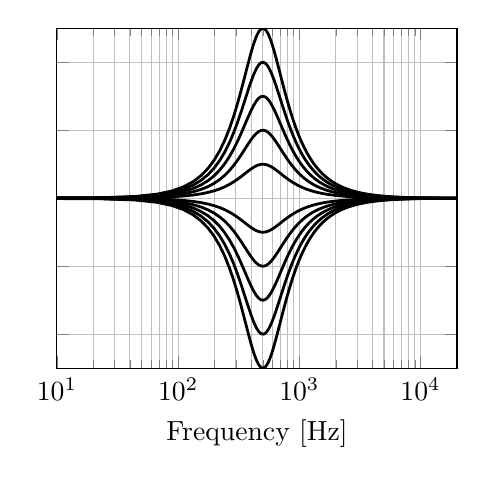
\begin{tikzpicture}

\begin{axis}[%
width=2in,
height=1.7in,
at={(1.011in,0.642in)},
scale only axis,
unbounded coords=jump,
xmode=log,
xmin=10,
xmax=20000,
xminorticks=true,
xlabel={Frequency [Hz]},
xmajorgrids,
xminorgrids,
ymin=-5,
ymax=5,
ymajorgrids,
yticklabels={\empty},
axis background/.style={fill=white}
]
\addplot [color=black,solid,line width=1.0pt,forget plot]
  table[row sep=crcr]{%
0.159154943091895	-6.76058748649941e-07\\
22.2100983353184	-0.0131792209368894\\
44.2610417275449	-0.0524977248528344\\
66.3119851197714	-0.11841679230081\\
88.362928511998	-0.211669051432683\\
110.413871904224	-0.333205011733822\\
132.464815296451	-0.484109559649171\\
154.515758688678	-0.665481734673923\\
176.566702080904	-0.878269124262541\\
198.617645473131	-1.12304794384191\\
220.668588865357	-1.39974140975748\\
242.719532257584	-1.70727360002581\\
264.77047564981	-2.04316550792318\\
286.821419042037	-2.40309707233203\\
308.872362434263	-2.78048666417806\\
330.92330582649	-3.16617946312176\\
352.974249218716	-3.54838395177158\\
375.025192610943	-3.91303292453086\\
397.076136003169	-4.24473261818622\\
419.127079395396	-4.5283490305297\\
441.178022787622	-4.75104178277422\\
463.228966179849	-4.90426585739014\\
485.279909572075	-4.98510523426627\\
507.330852964302	-4.99645778032346\\
529.381796356528	-4.94603264149291\\
551.432739748755	-4.84458336871655\\
573.483683140981	-4.70399811547319\\
595.534626533208	-4.53574532541999\\
617.585569925434	-4.34989277457256\\
639.636513317661	-4.15467260533357\\
661.687456709888	-3.95644161092091\\
683.738400102114	-3.75986886099448\\
705.789343494341	-3.56821959580025\\
727.840286886567	-3.38365293793705\\
749.891230278794	-3.20749084347987\\
771.94217367102	-3.04044188616636\\
793.993117063246	-2.88277805599617\\
816.044060455473	-2.73446957649289\\
838.0950038477	-2.59528507826158\\
860.145947239926	-2.46486452373853\\
882.196890632153	-2.34277136287792\\
904.247834024379	-2.22852920082203\\
926.298777416606	-2.12164710004197\\
948.349720808832	-2.02163664715798\\
970.400664201059	-1.92802311714397\\
992.451607593285	-1.84035245050419\\
1014.50255098551	-1.75819529287769\\
1036.55349437774	-1.68114900006291\\
1058.60443776996	-1.60883825677073\\
1080.65538116219	-1.54091477165098\\
1102.70632455442	-1.47705637642577\\
1124.75726794664	-1.41696575971351\\
1146.80821133887	-1.36036899618738\\
1168.8591547311	-1.30701398160059\\
1190.91009812332	-1.25666884844489\\
1212.96104151555	-1.20912041159592\\
1235.01198490778	-1.16417267535129\\
1257.0629283	-1.12164542067346\\
1279.11387169223	-1.08137288271449\\
1301.16481508446	-1.04320252270922\\
1323.21575847668	-1.00699389429935\\
1345.26670186891	-0.972617601724851\\
1367.31764526114	-0.939954345668409\\
1389.36858865336	-0.908894051585928\\
1411.41953204559	-0.879335074873854\\
1433.47047543782	-0.851183477071236\\
1455.52141883004	-0.824352367354457\\
1477.57236222227	-0.79876130378804\\
1499.6233056145	-0.774335749080402\\
1521.67424900672	-0.751006575931387\\
1543.72519239895	-0.728709617415332\\
1565.77613579117	-0.707385258205464\\
1587.8270791834	-0.686978062800027\\
1609.87802257563	-0.667436437248109\\
1631.92896596785	-0.648712321194434\\
1653.97990936008	-0.63076090735744\\
1676.03085275231	-0.613540385831363\\
1698.08179614453	-0.597011710852997\\
1720.13273953676	-0.581138387904987\\
1742.18368292899	-0.565886279234604\\
1764.23462632121	-0.55122342605671\\
1786.28556971344	-0.537119885880264\\
1808.33651310567	-0.523547583551689\\
1830.38745649789	-0.510480174746611\\
1852.43839989012	-0.497892920766762\\
1874.48934328235	-0.485762573611513\\
1896.54028667457	-0.474067270392776\\
1918.5912300668	-0.46278643625425\\
1940.64217345903	-0.451900695036433\\
1962.69311685125	-0.441391787002143\\
1984.74406024348	-0.431242493002901\\
2006.79500363571	-0.421436564525681\\
2028.84594702793	-0.411958659112447\\
2050.89689042016	-0.402794280692683\\
2072.94783381238	-0.393929724411967\\
2094.99877720461	-0.385352025578251\\
2117.04972059684	-0.377048912382813\\
2139.10066398906	-0.369008762083204\\
2161.15160738129	-0.36122056036485\\
2183.20255077352	-0.353673863622836\\
2205.25349416574	-0.346358763928689\\
2227.30443755797	-0.339265856467897\\
2249.3553809502	-0.332386209252483\\
2271.40632434242	-0.325711334930047\\
2293.45726773465	-0.319233164526537\\
2315.50821112688	-0.312944022973394\\
2337.5591545191	-0.306836606282591\\
2359.61009791133	-0.300903960245086\\
2381.66104130356	-0.295139460537923\\
2403.71198469578	-0.289536794135062\\
2425.76292808801	-0.284089941925841\\
2447.81387148024	-0.278793162452606\\
2469.86481487246	-0.273640976686083\\
2491.91575826469	-0.268628153764108\\
2513.96670165692	-0.263749697624593\\
2536.01764504914	-0.259000834469798\\
2558.06858844137	-0.254377001003188\\
2580.11953183359	-0.249873833385344\\
2602.17047522582	-0.245487156859324\\
2624.22141861805	-0.241212975999256\\
2646.27236201027	-0.237047465540311\\
2668.3233054025	-0.232986961750611\\
2690.37424879473	-0.229027954308841\\
2712.42519218695	-0.22516707865414\\
2734.47613557918	-0.221401108777172\\
2756.52707897141	-0.217726950423612\\
2778.57802236363	-0.214141634683295\\
2800.62896575586	-0.21064231194028\\
2822.67990914809	-0.207226246160801\\
2844.73085254031	-0.203890809497817\\
2866.78179593254	-0.200633477192242\\
2888.83273932477	-0.197451822752267\\
2910.88368271699	-0.194343513393737\\
2932.93462610922	-0.191306305725652\\
2954.98556950145	-0.18833804166551\\
2977.03651289367	-0.185436644570865\\
2999.0874562859	-0.182600115574331\\
3021.13839967812	-0.179826530109259\\
3043.18934307035	-0.177114034615617\\
3065.24028646258	-0.174460843414791\\
3087.2912298548	-0.171865235744072\\
3109.34217324703	-0.169325552941003\\
3131.39311663926	-0.166840195769516\\
3153.44406003148	-0.164407621879344\\
3175.49500342371	-0.162026343391462\\
3197.54594681594	-0.15969492460241\\
3219.59689020816	-0.157411979800488\\
3241.64783360039	-0.155176171188353\\
3263.69877699262	-0.152986206905404\\
3285.74972038484	-0.150840839145021\\
3307.80066377707	-0.148738862361136\\
3329.8516071693	-0.146679111559695\\
3351.90255056152	-0.144660460669986\\
3373.95349395375	-0.142681820992206\\
3396.00443734598	-0.140742139716381\\
3418.0553807382	-0.138840398509868\\
3440.10632413043	-0.136975612169069\\
3462.15726752266	-0.135146827332368\\
3484.20821091488	-0.133353121251166\\
3506.25915430711	-0.131593600615933\\
3528.31009769933	-0.12986740043444\\
3550.36104109156	-0.128173682959659\\
3572.41198448379	-0.126511636664843\\
3594.46292787601	-0.124880475263197\\
3616.51387126824	-0.123279436770246\\
3638.56481466047	-0.121707782606482\\
3660.61575805269	-0.120164796738688\\
3682.66670144492	-0.118649784857596\\
3704.71764483715	-0.117162073590609\\
3726.76858822937	-0.11570100974742\\
3748.8195316216	-0.114265959597325\\
3770.87047501383	-0.112856308176599\\
3792.92141840605	-0.111471458624427\\
3814.97236179828	-0.110110831546121\\
3837.02330519051	-0.108773864402451\\
3859.07424858273	-0.107460010923619\\
3881.12519197496	-0.106168740547036\\
3903.17613536719	-0.104899537877587\\
3925.22707875941	-0.103651902169416\\
3947.27802215164	-0.102425346828418\\
3969.32896554387	-0.101219398934121\\
3991.37990893609	-0.100033598780546\\
4013.43085232832	-0.0988674994348977\\
4035.48179572054	-0.0977206663133158\\
4057.53273911277	-0.0965926767730808\\
4079.583682505	-0.0954831197204738\\
4101.63462589722	-0.0943915952334715\\
4123.68556928945	-0.0933177141989435\\
4145.73651268168	-0.0922610979633481\\
4167.7874560739	-0.0912213779967311\\
4189.83839946613	-0.0901981955690886\\
4211.88934285836	-0.0891912014389205\\
4233.94028625058	-0.088200055553116\\
4255.99122964281	-0.0872244267580096\\
4278.04217303504	-0.0862639925209384\\
4300.09311642726	-0.0853184386618721\\
4322.14405981949	-0.0843874590949072\\
4344.19500321172	-0.08347075557881\\
4366.24594660394	-0.0825680374767743\\
4388.29688999617	-0.0816790215245414\\
4410.3478333884	-0.0808034316067297\\
4432.39877678062	-0.0799409985412489\\
4454.44972017285	-0.0790914598710184\\
4476.50066356508	-0.0782545596631032\\
4498.5516069573	-0.0774300483148113\\
4520.60255034953	-0.0766176823664857\\
4542.65349374176	-0.0758172243206505\\
4564.70443713398	-0.0750284424674619\\
4586.75538052621	-0.0742511107160672\\
4608.80632391843	-0.0734850084316106\\
4630.85726731066	-0.0727299202778217\\
4652.90821070289	-0.0719856360648209\\
4674.95915409511	-0.071251950602021\\
4697.01009748734	-0.0705286635559801\\
4719.06104087957	-0.0698155793128292\\
4741.11198427179	-0.0691125068453388\\
4763.16292766402	-0.0684192595843164\\
4785.21387105625	-0.067735655294117\\
4807.26481444847	-0.0670615159523321\\
4829.3157578407	-0.066396667633217\\
4851.36670123293	-0.0657409403950026\\
4873.41764462515	-0.065094168170689\\
4895.46858801738	-0.0644561886624192\\
4917.51953140961	-0.0638268432391416\\
4939.57047480183	-0.0632059768375282\\
4961.62141819406	-0.0625934378659752\\
4983.67236158629	-0.0619890781116794\\
5005.72330497851	-0.0613927526504849\\
5027.77424837074	-0.0608043197596858\\
5049.82519176296	-0.0602236408333477\\
5071.87613515519	-0.0596505803003807\\
5093.92707854742	-0.059085005545017\\
5115.97802193964	-0.0585267868297659\\
5138.02896533187	-0.0579757972206644\\
5160.0799087241	-0.0574319125148363\\
5182.13085211632	-0.0568950111701777\\
5204.18179550855	-0.0563649742371795\\
5226.23273890078	-0.0558416852927619\\
5248.283682293	-0.0553250303760851\\
5270.33462568523	-0.0548148979262707\\
5292.38556907746	-0.0543111787218987\\
5314.43651246968	-0.0538137658223576\\
5336.48745586191	-0.0533225545108585\\
5358.53839925414	-0.0528374422390656\\
5380.58934264636	-0.0523583285734361\\
5402.64028603859	-0.0518851151430275\\
5424.69122943082	-0.0514177055887714\\
5446.74217282304	-0.0509560055143406\\
5468.79311621527	-0.0504999224382133\\
5490.8440596075	-0.0500493657472836\\
5512.89500299972	-0.0496042466516528\\
5534.94594639195	-0.0491644781407773\\
5556.99688978417	-0.0487299749407539\\
5579.0478331764	-0.0483006534728901\\
5601.09877656863	-0.0478764318133789\\
5623.14971996085	-0.047457229654098\\
5645.20066335308	-0.0470429682644447\\
5667.25160674531	-0.046633570454297\\
5689.30255013753	-0.046228960537956\\
5711.35349352976	-0.0458290642990396\\
5733.40443692199	-0.0454338089563574\\
5755.45538031421	-0.0450431231307149\\
5777.50632370644	-0.0446569368125792\\
5799.55726709867	-0.0442751813306647\\
5821.60821049089	-0.0438977893212655\\
5843.65915388312	-0.0435246946985424\\
5865.71009727535	-0.0431558326254641\\
5887.76104066757	-0.0427911394855656\\
5909.8119840598	-0.0424305528554883\\
5931.86292745203	-0.0420740114781731\\
5953.91387084425	-0.0417214552368231\\
5975.96481423648	-0.0413728251294652\\
5998.0157576287	-0.0410280632442223\\
6020.06670102093	-0.040687112735244\\
6042.11764441316	-0.0403499177991763\\
6064.16858780538	-0.0400164236523232\\
6086.21953119761	-0.0396865765083395\\
6108.27047458984	-0.0393603235564917\\
6130.32141798206	-0.0390376129404871\\
6152.37236137429	-0.0387183937378632\\
6174.42330476652	-0.0384026159398126\\
6196.47424815874	-0.0380902304315816\\
6218.52519155097	-0.0377811889733917\\
6240.5761349432	-0.037475444181704\\
6262.62707833542	-0.0371729495111109\\
6284.67802172765	-0.0368736592365306\\
6306.72896511988	-0.0365775284359528\\
6328.7799085121	-0.0362845129735332\\
6350.83085190433	-0.0359945694831332\\
6372.88179529656	-0.0357076553522781\\
6394.93273868878	-0.0354237287064469\\
6416.98368208101	-0.0351427483937985\\
6439.03462547323	-0.0348646739702479\\
6461.08556886546	-0.0345894656849021\\
6483.13651225769	-0.0343170844658215\\
6505.18745564992	-0.034047491906158\\
6527.23839904214	-0.0337806502506132\\
6549.28934243437	-0.0335165223821964\\
6571.34028582659	-0.033255071809307\\
6593.39122921882	-0.0329962626531396\\
6615.44217261105	-0.0327400596353587\\
6637.49311600327	-0.0324864280660732\\
6659.5440593955	-0.032235333832087\\
6681.59500278773	-0.0319867433854414\\
6703.64594617995	-0.0317406237321766\\
6725.69688957218	-0.0314969424214256\\
6747.74783296441	-0.0312556675346648\\
6769.79877635663	-0.0310167676753026\\
6791.84971974886	-0.0307802119584527\\
6813.90066314109	-0.03054597000095\\
6835.95160653331	-0.0303140119115945\\
6858.00254992554	-0.0300843082816373\\
6880.05349331777	-0.0298568301754174\\
6902.10443670999	-0.0296315491213179\\
6924.15538010222	-0.0294084371027988\\
6946.20632349445	-0.0291874665497352\\
6968.25726688667	-0.028968610329874\\
6990.3082102789	-0.0287518417405311\\
7012.35915367112	-0.0285371345004376\\
7034.41009706335	-0.0283244627417999\\
7056.46104045558	-0.0281138010024931\\
7078.5119838478	-0.027905124218462\\
7100.56292724003	-0.0276984077162638\\
7122.61387063226	-0.0274936272057908\\
7144.66481402448	-0.0272907587731334\\
7166.71575741671	-0.0270897788736167\\
7188.76670080894	-0.0268906643249765\\
7210.81764420116	-0.0266933923006679\\
7232.86858759339	-0.0264979403233694\\
7254.91953098562	-0.0263042862585293\\
7276.97047437784	-0.0261124083081841\\
7299.02141777007	-0.0259222850047748\\
7321.0723611623	-0.0257338952051611\\
7343.12330455452	-0.0255472180847949\\
7365.17424794675	-0.0253622331319179\\
7387.22519133898	-0.0251789201419941\\
7409.2761347312	-0.0249972592121518\\
7431.32707812343	-0.0248172307358416\\
7453.37802151566	-0.0246388153975107\\
7475.42896490788	-0.0244619941674694\\
7497.47990830011	-0.0242867482968183\\
7519.53085169233	-0.0241130593124739\\
7541.58179508456	-0.0239409090123406\\
7563.63273847679	-0.0237702794605314\\
7585.68368186901	-0.0236011529827131\\
7607.73462526124	-0.0234335121615577\\
7629.78556865347	-0.0232673398322313\\
7651.83651204569	-0.0231026190780744\\
7673.88745543792	-0.0229393332262569\\
7695.93839883015	-0.0227774658435762\\
7717.98934222237	-0.0226170007323667\\
7740.0402856146	-0.0224579219264349\\
7762.09122900683	-0.0223002136871126\\
7784.14217239905	-0.0221438604993666\\
7806.19311579128	-0.0219888470680077\\
7828.24405918351	-0.0218351583139384\\
7850.29500257573	-0.021682779370549\\
7872.34594596796	-0.0215316955800826\\
7894.39688936019	-0.0213818924901472\\
7916.44783275241	-0.0212333558502747\\
7938.49877614464	-0.0210860716085471\\
7960.54971953686	-0.0209400259082625\\
7982.60066292909	-0.0207952050847285\\
8004.65160632132	-0.0206515956620369\\
8026.70254971355	-0.0205091843499887\\
8048.75349310577	-0.0203679580409845\\
8070.804436498	-0.0202279038070611\\
8092.85537989022	-0.0200890088969181\\
8114.90632328245	-0.0199512607330394\\
8136.95726667468	-0.0198146469088783\\
8159.0082100669	-0.0196791551860416\\
8181.05915345913	-0.0195447734915907\\
8203.11009685136	-0.0194114899153467\\
8225.16104024358	-0.0192792927072835\\
8247.21198363581	-0.0191481702749289\\
8269.26292702804	-0.019018111180865\\
8291.31387042026	-0.0188891041402182\\
8313.36481381249	-0.0187611380182463\\
8335.41575720472	-0.018634201827929\\
8357.46670059694	-0.0185082847276507\\
8379.51764398917	-0.0183833760188777\\
8401.56858738139	-0.0182594651438925\\
8423.61953077362	-0.0181365416836057\\
8445.67047416585	-0.0180145953553507\\
8467.72141755808	-0.0178936160107524\\
8489.7723609503	-0.01777359363365\\
8511.82330434253	-0.0176545183379994\\
8533.87424773476	-0.0175363803658934\\
8555.92519112698	-0.0174191700855315\\
8577.97613451921	-0.0173028779893163\\
8600.02707791143	-0.0171874946918811\\
8622.07802130366	-0.0170730109282802\\
8644.12896469589	-0.0169594175520801\\
8666.17990808811	-0.0168467055335699\\
8688.23085148034	-0.0167348659579981\\
8710.28179487257	-0.0166238900237643\\
8732.33273826479	-0.0165137690407902\\
8754.38368165702	-0.0164044944287411\\
8776.43462504925	-0.016296057715426\\
8798.48556844147	-0.016188450535137\\
8820.5365118337	-0.0160816646270748\\
8842.58745522593	-0.0159756918337419\\
8864.63839861815	-0.0158705240994315\\
8886.68934201038	-0.0157661534686908\\
8908.74028540261	-0.0156625720848214\\
8930.79122879483	-0.0155597721884322\\
8952.84217218706	-0.0154577461159968\\
8974.89311557929	-0.0153564862984107\\
8996.94405897151	-0.0152559852596341\\
9018.99500236374	-0.0151562356152984\\
9041.04594575596	-0.0150572300713867\\
9063.09688914819	-0.0149589614228896\\
9085.14783254042	-0.0148614225525123\\
9107.19877593265	-0.0147646064294068\\
9129.24971932487	-0.0146685061079002\\
9151.3006627171	-0.0145731147262855\\
9173.35160610933	-0.0144784255055837\\
9195.40254950155	-0.0143844317483612\\
9217.45349289378	-0.0142911268375606\\
9239.504436286	-0.014198504235347\\
9261.55537967823	-0.0141065574819651\\
9283.60632307046	-0.0140152801946349\\
9305.65726646268	-0.0139246660664474\\
9327.70820985491	-0.0138347088652974\\
9349.75915324714	-0.0137454024328043\\
9371.81009663936	-0.0136567406832995\\
9393.86104003159	-0.013568717602767\\
9415.91198342382	-0.0134813272478564\\
9437.96292681604	-0.0133945637448779\\
9460.01387020827	-0.0133084212888473\\
9482.06481360049	-0.0132228941425048\\
9504.11575699272	-0.0131379766353668\\
9526.16670038495	-0.0130536631628207\\
9548.21764377718	-0.0129699481852019\\
9570.2685871694	-0.0128868262268774\\
9592.31953056163	-0.0128042918753833\\
9614.37047395386	-0.0127223397805388\\
9636.42141734608	-0.0126409646536078\\
9658.47236073831	-0.012560161266429\\
9680.52330413053	-0.0124799244506211\\
9702.57424752276	-0.0124002490967236\\
9724.62519091499	-0.0123211301534498\\
9746.67613430721	-0.0122425626268338\\
9768.72707769944	-0.0121645415795077\\
9790.77802109167	-0.0120870621298976\\
9812.82896448389	-0.012010119451484\\
9834.87990787612	-0.0119337087720849\\
9856.93085126835	-0.0118578253730638\\
9878.98179466057	-0.0117824645886824\\
9901.0327380528	-0.0117076218053527\\
9923.08368144502	-0.0116332924609302\\
9945.13462483725	-0.0115594720440696\\
9967.18556822948	-0.0114861560935149\\
9989.23651162171	-0.011413340197457\\
10011.2874550139	-0.0113410199928505\\
10033.3383984062	-0.0112691911648227\\
10055.3893417984	-0.0111978494459696\\
10077.4402851906	-0.0111269906157978\\
10099.4912285828	-0.0110566105000603\\
10121.5421719751	-0.0109867049701819\\
10143.5931153673	-0.0109172699426514\\
10165.6440587595	-0.010848301378432\\
10187.6950021517	-0.0107797952823891\\
10209.745945544	-0.0107117477027208\\
10231.7968889362	-0.0106441547303796\\
10253.8478323284	-0.010577012498562\\
10275.8987757206	-0.0105103171821195\\
10297.9497191129	-0.0104440649970481\\
10320.0006625051	-0.0103782521999426\\
10342.0516058973	-0.0103128750875041\\
10364.1025492896	-0.0102479299960068\\
10386.1534926818	-0.0101834133007851\\
10408.204436074	-0.0101193214157725\\
10430.2553794662	-0.0100556507929722\\
10452.3063228585	-0.00999239792199761\\
10474.3572662507	-0.00992955932958718\\
10496.4082096429	-0.00986713157915755\\
10518.4591530351	-0.00980511127030232\\
10540.5100964274	-0.00974349503837019\\
10562.5610398196	-0.00968227955400936\\
10584.6119832118	-0.00962146152272257\\
10606.662926604	-0.00956103768443184\\
10628.7138699963	-0.00950100481305688\\
10650.7648133885	-0.00944135971607893\\
10672.8157567807	-0.00938209923413756\\
10694.866700173	-0.00932322024061692\\
10716.9176435652	-0.00926471964124546\\
10738.9685869574	-0.00920659437367845\\
10761.0195303496	-0.00914884140713545\\
10783.0704737419	-0.00909145774198676\\
10805.1214171341	-0.00903444040937943\\
10827.1723605263	-0.00897778647087491\\
10849.2233039185	-0.00892149301805976\\
10871.2742473108	-0.00886555717219017\\
10893.325190703	-0.00880997608382872\\
10915.3761340952	-0.00875474693248902\\
10937.4270774874	-0.00869986692628807\\
10959.4780208797	-0.00864533330159574\\
10981.5289642719	-0.00859114332269684\\
11003.5799076641	-0.00853729428146969\\
11025.6308510564	-0.00848378349702604\\
11047.6817944486	-0.00843060831540227\\
11069.7327378408	-0.00837776610924956\\
11091.783681233	-0.00832525427749527\\
11113.8346246253	-0.00827307024503219\\
11135.8855680175	-0.0082212114624311\\
11157.9365114097	-0.00816967540561091\\
11179.9874548019	-0.00811845957554634\\
11202.0383981942	-0.00806756149799608\\
11224.0893415864	-0.00801697872316326\\
11246.1402849786	-0.00796670882545837\\
11268.1912283708	-0.00791674940318493\\
11290.2421717631	-0.00786709807825225\\
11312.2931151553	-0.00781775249593744\\
11334.3440585475	-0.00776871032457696\\
11356.3950019397	-0.00771996925530941\\
11378.445945332	-0.00767152700182116\\
11400.4968887242	-0.00762338130007278\\
11422.5478321164	-0.00757552990803706\\
11444.5987755087	-0.00752797060546308\\
11466.6497189009	-0.00748070119360945\\
11488.7006622931	-0.00743371949500169\\
11510.7516056853	-0.00738702335318485\\
11532.8025490776	-0.00734061063249828\\
11554.8534924698	-0.00729447921780993\\
11576.904435862	-0.00724862701431728\\
11598.9553792542	-0.00720305194727397\\
11621.0063226465	-0.00715775196180327\\
11643.0572660387	-0.00711272502263729\\
11665.1082094309	-0.0070679691139267\\
11687.1591528231	-0.00702348223900411\\
11709.2100962154	-0.00697926242015319\\
11731.2610396076	-0.00693530769843398\\
11753.3119829998	-0.00689161613342979\\
11775.3629263921	-0.0068481858030735\\
11797.4138697843	-0.00680501480341871\\
11819.4648131765	-0.00676210124845824\\
11841.5157565687	-0.0067194432698896\\
11863.566699961	-0.00667703901697696\\
11885.6176433532	-0.00663488665627607\\
11907.6685867454	-0.00659298437152527\\
11929.7195301376	-0.00655133036339261\\
11951.7704735299	-0.00650992284932155\\
11973.8214169221	-0.00646876006333213\\
11995.8723603143	-0.00642784025584744\\
12017.9233037065	-0.0063871616935141\\
12039.9742470988	-0.00634672265900752\\
12062.025190491	-0.0063065214508843\\
12084.0761338832	-0.00626655638338745\\
12106.1270772755	-0.00622682578626416\\
12128.1780206677	-0.00618732800464624\\
12150.2289640599	-0.00614806139883806\\
12172.2799074521	-0.006109024344142\\
12194.3308508444	-0.0060702152307622\\
12216.3817942366	-0.0060316324635712\\
12238.4327376288	-0.00599327446198761\\
12260.483681021	-0.00595513965982487\\
12282.5346244133	-0.00591722650510521\\
12304.5855678055	-0.00587953345994705\\
12326.6365111977	-0.00584205900039248\\
12348.6874545899	-0.00580480161625222\\
12370.7383979822	-0.00576775981096984\\
12392.7893413744	-0.00573093210148119\\
12414.8402847666	-0.00569431701806508\\
12436.8912281588	-0.00565791310419124\\
12458.9421715511	-0.00562171891639994\\
12480.9931149433	-0.00558573302416052\\
12503.0440583355	-0.00554995400971641\\
12525.0950017278	-0.00551438046796195\\
12547.14594512	-0.00547901100632311\\
12569.1968885122	-0.00544384424463148\\
12591.2478319044	-0.00540887881493552\\
12613.2987752967	-0.00537411336145271\\
12635.3497186889	-0.00533954654038666\\
12657.4006620811	-0.00530517701982325\\
12679.4516054733	-0.00527100347960954\\
12701.5025488656	-0.00523702461122392\\
12723.5534922578	-0.00520323911766844\\
12745.60443565	-0.00516964571332847\\
12767.6553790422	-0.00513624312386695\\
12789.7063224345	-0.00510303008612451\\
12811.7572658267	-0.00507000534797527\\
12833.8082092189	-0.00503716766822786\\
12855.8591526112	-0.00500451581652468\\
12877.9100960034	-0.00497204857320914\\
12899.9610393956	-0.00493976472923269\\
12922.0119827878	-0.00490766308603462\\
12944.0629261801	-0.00487574245545192\\
12966.1138695723	-0.00484400165959924\\
12988.1648129645	-0.00481243953076319\\
13010.2157563567	-0.00478105491132578\\
13032.266699749	-0.00474984665361827\\
13054.3176431412	-0.00471881361986574\\
13076.3685865334	-0.00468795468205647\\
13098.4195299256	-0.00465726872186432\\
13120.4704733179	-0.00462675463053064\\
13142.5214167101	-0.00459641130879633\\
13164.5723601023	-0.00456623766677219\\
13186.6233034945	-0.00453623262387868\\
13208.6742468868	-0.00450639510874239\\
13230.725190279	-0.00447672405908462\\
13252.7761336712	-0.00444721842167865\\
13274.8270770635	-0.00441787715218726\\
13296.8780204557	-0.00438869921516429\\
13318.9289638479	-0.00435968358388069\\
13340.9799072401	-0.00433082924030095\\
13363.0308506324	-0.00430213517497188\\
13385.0817940246	-0.00427360038694506\\
13407.1327374168	-0.00424522388368486\\
13429.183680809	-0.00421700468099384\\
13451.2346242013	-0.00418894180292466\\
13473.2855675935	-0.004161034281717\\
13495.3365109857	-0.00413328115769699\\
13517.3874543779	-0.00410568147920546\\
13539.4383977702	-0.00407823430253397\\
13561.4893411624	-0.00405093869182713\\
13583.5402845546	-0.00402379371902533\\
13605.5912279469	-0.00399679846376511\\
13627.6421713391	-0.00396995201334222\\
13649.6931147313	-0.00394325346260231\\
13671.7440581235	-0.00391670191387702\\
13693.7950015158	-0.00389029647694701\\
13715.845944908	-0.00386403626890859\\
13737.8968883002	-0.00383792041416283\\
13759.9478316924	-0.00381194804431403\\
13781.9987750847	-0.00378611829810093\\
13804.0497184769	-0.00376043032134344\\
13826.1006618691	-0.0037348832668758\\
13848.1516052613	-0.00370947629445472\\
13870.2025486536	-0.00368420857073402\\
13892.2534920458	-0.00365907926917181\\
13914.304435438	-0.0036340875699714\\
13936.3553788303	-0.00360923266001065\\
13958.4063222225	-0.00358451373280894\\
13980.4572656147	-0.00355992998843916\\
14002.5082090069	-0.00353548063346287\\
14024.5591523992	-0.00351116488089436\\
14046.6100957914	-0.00348698195011364\\
14068.6610391836	-0.00346293106682862\\
14090.7119825758	-0.00343901146300732\\
14112.7629259681	-0.00341522237681791\\
14134.8138693603	-0.00339156305256385\\
14156.8648127525	-0.00336803274067116\\
14178.9157561447	-0.00334463069756279\\
14200.966699537	-0.00332135618566234\\
14223.0176429292	-0.00329820847330216\\
14245.0685863214	-0.00327518683469814\\
14267.1195297136	-0.00325229054986846\\
14289.1704731059	-0.00322951890459963\\
14311.2214164981	-0.00320687119038946\\
14333.2723598903	-0.00318434670439759\\
14355.3233032826	-0.00316194474938367\\
14377.3742466748	-0.00313966463366757\\
14399.425190067	-0.00311750567107137\\
14421.4761334592	-0.00309546718088253\\
14443.5270768515	-0.00307354848778713\\
14465.5780202437	-0.00305174892183792\\
14487.6289636359	-0.0030300678183924\\
14509.6799070281	-0.00300850451807407\\
14531.7308504204	-0.00298705836672406\\
14553.7817938126	-0.00296572871535466\\
14575.8327372048	-0.002944514920099\\
14597.883680597	-0.00292341634217523\\
14619.9346239893	-0.00290243234782366\\
14641.9855673815	-0.00288156230828539\\
14664.0365107737	-0.00286080559973947\\
14686.087454166	-0.00284016160327188\\
14708.1383975582	-0.00281962970482236\\
14730.1893409504	-0.0027992092951418\\
14752.2402843426	-0.00277889976977475\\
14774.2912277349	-0.00275870052896286\\
14796.3421711271	-0.00273861097768325\\
14818.3931145193	-0.00271863052551246\\
14840.4440579115	-0.00269875858668318\\
14862.4950013038	-0.00267899457995874\\
14884.545944696	-0.00265933792865997\\
14906.5968880882	-0.00263978806058411\\
14928.6478314804	-0.00262034440796698\\
14950.6987748727	-0.00260100640749164\\
14972.7497182649	-0.00258177350019654\\
14994.8006616571	-0.00256264513144172\\
15016.8516050494	-0.00254362075091154\\
15038.9025484416	-0.00252469981254994\\
15060.9534918338	-0.00250588177451792\\
15083.004435226	-0.00248716609917605\\
15105.0553786183	-0.00246855225303803\\
15127.1063220105	-0.00245003970673108\\
15149.1572654027	-0.00243162793497844\\
15171.2082087949	-0.00241331641654237\\
15193.2591521872	-0.00239510463422018\\
15215.3100955794	-0.00237699207476505\\
15237.3610389716	-0.00235897822890036\\
15259.4119823638	-0.00234106259125019\\
15281.4629257561	-0.00232324466033434\\
15303.5138691483	-0.00230552393852394\\
15325.5648125405	-0.00228789993199014\\
15347.6157559327	-0.00227037215070604\\
15369.666699325	-0.00225294010839925\\
15391.7176427172	-0.0022356033225094\\
15413.7685861094	-0.00221836131419096\\
15435.8195295017	-0.0022012136082369\\
15457.8704728939	-0.00218415973308443\\
15479.9214162861	-0.00216719922077341\\
15501.9723596783	-0.00215033160690674\\
15524.0233030706	-0.0021335564306464\\
15546.0742464628	-0.00211687323465357\\
15568.125189855	-0.00210028156507892\\
15590.1761332472	-0.0020837809715403\\
15612.2270766395	-0.00206737100706964\\
15634.2780200317	-0.00205105122810805\\
15656.3289634239	-0.00203482119446716\\
15678.3799068161	-0.00201868046930973\\
15700.4308502084	-0.00200262861911487\\
15722.4817936006	-0.00198666521364322\\
15744.5327369928	-0.00197078982593788\\
15766.5836803851	-0.00195500203226836\\
15788.6346237773	-0.00193930141213533\\
15810.6855671695	-0.00192368754820595\\
15832.7365105617	-0.00190816002632725\\
15854.787453954	-0.00189271843546827\\
15876.8383973462	-0.00187736236772089\\
15898.8893407384	-0.00186209141826118\\
15920.9402841306	-0.00184690518533106\\
15942.9912275229	-0.00183180327021022\\
15965.0421709151	-0.00181678527718905\\
15987.0931143073	-0.00180185081355507\\
16009.1440576995	-0.00178699948955626\\
16031.1950010918	-0.0017722309183961\\
16053.245944484	-0.00175754471619595\\
16075.2968878762	-0.00174294050196315\\
16097.3478312684	-0.00172841789759863\\
16119.3987746607	-0.00171397652784966\\
16141.4497180529	-0.00169961602029045\\
16163.5006614451	-0.00168533600532017\\
16185.5516048374	-0.00167113611610601\\
16207.6025482296	-0.0016570159885966\\
16229.6534916218	-0.00164297526148339\\
16251.704435014	-0.00162901357616874\\
16273.7553784063	-0.00161513057678328\\
16295.8063217985	-0.00160132591011731\\
16317.8572651907	-0.00158759922563816\\
16339.9082085829	-0.00157395017544285\\
16361.9591519752	-0.00156037841426575\\
16384.0100953674	-0.00154688359943034\\
16406.0610387596	-0.0015334653908462\\
16428.1119821518	-0.00152012345099651\\
16450.1629255441	-0.0015068574448868\\
16472.2138689363	-0.00149366704006422\\
16494.2648123285	-0.00148055190657606\\
16516.3157557208	-0.00146751171695901\\
16538.366699113	-0.00145454614621412\\
16560.4176425052	-0.0014416548718067\\
16582.4685858974	-0.00142883757360552\\
16604.5195292897	-0.00141609393392619\\
16626.5704726819	-0.00140342363745297\\
16648.6214160741	-0.00139082637127441\\
16670.6723594663	-0.00137830182481291\\
16692.7233028586	-0.00136584968985843\\
16714.7742462508	-0.00135346966051252\\
16736.825189643	-0.00134116143319501\\
16758.8761330352	-0.00132892470661214\\
16780.9270764275	-0.00131675918175749\\
16802.9780198197	-0.00130466456186374\\
16825.0289632119	-0.00129264055243054\\
16847.0799066042	-0.00128068686117054\\
16869.1308499964	-0.00126880319801216\\
16891.1817933886	-0.00125698927507648\\
16913.2327367808	-0.00124524480666653\\
16935.2836801731	-0.0012335695092509\\
16957.3346235653	-0.00122196310144343\\
16979.3855669575	-0.00121042530399354\\
17001.4365103497	-0.00119895583977169\\
17023.487453742	-0.00118755443374627\\
17045.5383971342	-0.00117622081297963\\
17067.5893405264	-0.00116495470660107\\
17089.6402839186	-0.00115375584580684\\
17111.6912273109	-0.00114262396384075\\
17133.7421707031	-0.00113155879595368\\
17155.7931140953	-0.00112056007945465\\
17177.8440574875	-0.00110962755361048\\
17199.8950008798	-0.00109876095971711\\
17221.945944272	-0.00108796004101377\\
17243.9968876642	-0.0010772245427244\\
17266.0478310565	-0.00106655421199683\\
17288.0987744487	-0.00105594879794235\\
17310.1497178409	-0.00104540805157102\\
17332.2006612331	-0.00103493172581286\\
17354.2516046254	-0.00102451957549179\\
17376.3025480176	-0.00101417135731306\\
17398.3534914098	-0.00100388682984684\\
17420.404434802	-0.000993665753529126\\
17442.4553781943	-0.000983507890641474\\
17464.5063215865	-0.000973413005287831\\
17486.5572649787	-0.000963380863402214\\
17508.6082083709	-0.000953411232728432\\
17530.6591517632	-0.000943503882799807\\
17552.7100951554	-0.000933658584931428\\
17574.7610385476	-0.000923875112224953\\
17596.8119819399	-0.000914153239529998\\
17618.8629253321	-0.000904492743451831\\
17640.9138687243	-0.000894893402331094\\
17662.9648121165	-0.000885354996240883\\
17685.0157555088	-0.000875877306969361\\
17707.066698901	-0.000866460117993699\\
17729.1176422932	-0.000857103214512839\\
17751.1685856854	-0.000847806383381889\\
17773.2195290777	-0.00083856941314103\\
17795.2704724699	-0.000829392093997176\\
17817.3214158621	-0.000820274217790186\\
17839.3723592543	-0.000811215578015994\\
17861.4233026466	-0.000802215969793795\\
17883.4742460388	-0.000793275189867949\\
17905.525189431	-0.000784393036588671\\
17927.5761328233	-0.000775569309891761\\
17949.6270762155	-0.000766803811336187\\
17971.6780196077	-0.000758096344026916\\
17993.7289629999	-0.000749446712657327\\
18015.7799063922	-0.000740854723472538\\
18037.8308497844	-0.000732320184276142\\
18059.8817931766	-0.000723842904406072\\
18081.9327365688	-0.000715422694732654\\
18103.9836799611	-0.000707059367654728\\
18126.0346233533	-0.00069875273707263\\
18148.0855667455	-0.000690502618403593\\
18170.1365101377	-0.000682308828549915\\
18192.18745353	-0.000674171185911465\\
18214.2383969222	-0.000666089510346135\\
18236.2893403144	-0.000658063623202602\\
18258.3402837066	-0.000650093347270165\\
18280.3912270989	-0.000642178506802838\\
18302.4421704911	-0.000634318927494255\\
18324.4931138833	-0.000626514436460296\\
18346.5440572756	-0.000618764862259317\\
18368.5950006678	-0.00061107003485935\\
18390.64594406	-0.000603429785639046\\
18412.6968874522	-0.000595843947370299\\
18434.7478308445	-0.000588312354236554\\
18456.7987742367	-0.000580834841779749\\
18478.8497176289	-0.000573411246949484\\
18500.9006610211	-0.000566041408043208\\
18522.9516044134	-0.000558725164728391\\
18545.0025478056	-0.00055146235802225\\
18567.0534911978	-0.000544252830291737\\
18589.10443459	-0.00053709642524677\\
18611.1553779823	-0.000529992987920935\\
18633.2063213745	-0.000522942364672432\\
18655.2572647667	-0.000515944403192738\\
18677.308208159	-0.000508998952453556\\
18699.3591515512	-0.000502105862755015\\
18721.4100949434	-0.000495264985682264\\
18743.4610383356	-0.000488476174108345\\
18765.5119817279	-0.000481739282202863\\
18787.5629251201	-0.000475054165382787\\
18809.6138685123	-0.00046842068035294\\
18831.6648119045	-0.000461838685074162\\
18853.7157552968	-0.000455308038771012\\
18875.766698689	-0.000448828601896073\\
18897.8176420812	-0.000442400236164655\\
18919.8685854734	-0.000436022804516209\\
18941.9195288657	-0.000429696171122992\\
18963.9704722579	-0.000423420201380415\\
18986.0214156501	-0.000417194761884842\\
19008.0723590424	-0.000411019720472163\\
19030.1233024346	-0.000404894946157017\\
19052.1742458268	-0.00039882030916847\\
19074.225189219	-0.000392795680922028\\
19096.2761326113	-0.000386820934009027\\
19118.3270760035	-0.000380895942214936\\
19140.3780193957	-0.000375020580500063\\
19162.4289627879	-0.00036919472498315\\
19184.4799061802	-0.000363418252951002\\
19206.5308495724	-0.000357691042851729\\
19228.5817929646	-0.000352012974282196\\
19250.6327363568	-0.000346383927985123\\
19272.6836797491	-0.000340803785848105\\
19294.7346231413	-0.000335272430879495\\
19316.7855665335	-0.000329789747247936\\
19338.8365099257	-0.000324355620212911\\
19360.887453318	-0.00031896993617874\\
19382.9383967102	-0.00031363258265214\\
19404.9893401024	-0.000308343448258605\\
19427.0402834947	-0.000303102422716364\\
19449.0912268869	-0.000297909396850832\\
19471.1421702791	-0.000292764262583032\\
19493.1931136713	-0.000287666912921868\\
19515.2440570636	-0.000282617241962191\\
19537.2950004558	-0.000277615144873212\\
19559.345943848	-0.000272660517910071\\
19581.3968872402	-0.000267753258391645\\
19603.4478306325	-0.000262893264701504\\
19625.4987740247	-0.000258080436297548\\
19647.5497174169	-0.000253314673678243\\
19669.6006608091	-0.000248595878405758\\
19691.6516042014	-0.000243923953092459\\
19713.7025475936	-0.000239298801383539\\
19735.7534909858	-0.000234720327970511\\
19757.8044343781	-0.000230188438584451\\
19779.8553777703	-0.00022570303998249\\
19801.9063211625	-0.000221264039954555\\
19823.9572645547	-0.000216871347302147\\
19846.008207947	-0.000212524871864369\\
19868.0591513392	-0.00020822452447549\\
19890.1100947314	-0.000203970216997724\\
19912.1610381236	-0.000199761862292292\\
19934.2119815159	-0.000195599374224236\\
19956.2629249081	-0.00019148266765856\\
19978.3138683003	-0.00018741165845925\\
20000.3648116925	-0.000183386263481559\\
20022.4157550848	-0.000179406400561392\\
20044.466698477	-0.000175471988539404\\
20066.5176418692	-0.000171582947213744\\
20088.5685852615	-0.000167739197376693\\
20110.6195286537	-0.000163940660789585\\
20132.6704720459	-0.000160187260186658\\
20154.7214154381	-0.000156478919269259\\
20176.7723588304	-0.000152815562701022\\
20198.8233022226	-0.000149197116105928\\
20220.8742456148	-0.000145623506078909\\
20242.925189007	-0.000142094660150163\\
20264.9761323993	-0.000138610506812147\\
20287.0270757915	-0.000135170975502214\\
20309.0780191837	-0.000131775996611289\\
20331.1289625759	-0.000128425501461681\\
20353.1799059682	-0.000125119422317686\\
20375.2308493604	-0.000121857692379795\\
20397.2817927526	-0.000118640245794336\\
20419.3327361449	-0.000115467017622605\\
20441.3836795371	-0.000112337943854363\\
20463.4346229293	-0.000109252961424228\\
20485.4855663215	-0.0001062120081567\\
20507.5365097138	-0.000103215022824014\\
20529.587453106	-0.000100261945105641\\
20551.6383964982	-9.73527155902028e-05\\
20573.6893398904	-9.44872757899398e-05\\
20595.7402832827	-9.16655681137005e-05\\
20617.7912266749	-8.88875358823687e-05\\
20639.8421700671	-8.61531233346445e-05\\
20661.8931134593	-8.34622755855737e-05\\
20683.9440568516	-8.08149386728316e-05\\
20705.9950002438	-7.82110595104313e-05\\
20728.045943636	-7.5650585932114e-05\\
20750.0968870282	-7.31334666498793e-05\\
20772.1478304205	-7.065965126266e-05\\
20794.1987738127	-6.82290902640331e-05\\
20816.2497172049	-6.58417350422159e-05\\
20838.3006605972	-6.3497537857883e-05\\
20860.3516039894	-6.11964518489838e-05\\
20882.4025473816	-5.89384310509907e-05\\
20904.4534907738	-5.67234303689295e-05\\
20926.5044341661	-5.45514055821978e-05\\
20948.5553775583	-5.24223133532407e-05\\
20970.6063209505	-5.03361112034393e-05\\
20992.6572643427	-4.829275753818e-05\\
21014.708207735	-4.62922116208148e-05\\
21036.7591511272	-4.43344335986949e-05\\
21058.8100945194	-4.241938446363e-05\\
21080.8610379116	-4.0547026089495e-05\\
21102.9119813039	-3.87173211994391e-05\\
21124.9629246961	-3.69302333919205e-05\\
21147.0138680883	-3.51857271137023e-05\\
21169.0648114806	-3.34837676637073e-05\\
21191.1157548728	-3.18243212219448e-05\\
21213.166698265	-3.02073547877921e-05\\
21235.2176416572	-2.86328362513511e-05\\
21257.2685850495	-2.71007343278727e-05\\
21279.3195284417	-2.56110185905411e-05\\
21301.3704718339	-2.41636594714358e-05\\
21323.4214152261	-2.27586282403146e-05\\
21345.4723586184	-2.13958970152188e-05\\
21367.5233020106	-2.00754387653644e-05\\
21389.5742454028	-1.87972273024609e-05\\
21411.625188795	-1.75612372816737e-05\\
21433.6761321873	-1.63674441987295e-05\\
21455.7270755795	-1.52158243937719e-05\\
21477.7780189717	-1.41063550465375e-05\\
21499.8289623639	-1.30390141763546e-05\\
21521.8799057562	-1.20137806373203e-05\\
21543.9308491484	-1.10306341346917e-05\\
21565.9817925406	-1.00895551911336e-05\\
21588.0327359329	-9.19052518239714e-06\\
21610.0836793251	-8.33352630838827e-06\\
21632.1346227173	-7.51854161245335e-06\\
21654.1855661095	-6.74555496498421e-06\\
21676.2365095018	-6.01455106823864e-06\\
21698.287452894	-5.32551547273282e-06\\
21720.3383962862	-4.67843453384557e-06\\
21742.3893396784	-4.07329546678401e-06\\
21764.4402830707	-3.51008629643762e-06\\
21786.4912264629	-2.98879588630716e-06\\
21808.5421698551	-2.50941393753958e-06\\
21830.5931132473	-2.07193095903309e-06\\
21852.6440566396	-1.67633831179556e-06\\
21874.6950000318	-1.32262817904972e-06\\
21896.745943424	-1.01079356044665e-06\\
21918.7968868162	-7.40828298102117e-07\\
21940.8478302085	-5.12727055380893e-07\\
21962.8987736007	-3.26485321718045e-07\\
21984.9497169929	-1.8209942419052e-07\\
22007.0006603852	-7.9566499551384e-08\\
22029.0516037774	-1.88845279810809e-08\\
};
\addplot [color=black,solid,line width=1.0pt,forget plot]
  table[row sep=crcr]{%
0.159154943091895	-5.30385936728065e-07\\
22.2100983353184	-0.0103410572217024\\
44.2610417275449	-0.0412112309620665\\
66.3119851197714	-0.0930290614734396\\
88.362928511998	-0.166463651266814\\
110.413871904224	-0.262391902518404\\
132.464815296451	-0.381829910935425\\
154.515758688678	-0.525831298136537\\
176.566702080904	-0.695343283508616\\
198.617645473131	-0.891011082395193\\
220.668588865357	-1.11292330480837\\
242.719532257584	-1.36029696029076\\
264.77047564981	-1.63111241926521\\
286.821419042037	-1.92172826163148\\
308.872362434263	-2.22653436456187\\
330.92330582649	-2.53773652795184\\
352.974249218716	-2.84539798426695\\
375.025192610943	-3.1378718908734\\
397.076136003169	-3.40271425294197\\
419.127079395396	-3.628044078203\\
441.178022787622	-3.80413009428296\\
463.228966179849	-3.92481014356308\\
485.279909572075	-3.98831260701176\\
507.330852964302	-3.99722091798198\\
529.381796356528	-3.95763436740331\\
551.432739748755	-3.87785223831019\\
573.483683140981	-3.76699834465905\\
595.534626533208	-3.63390486714672\\
617.585569925434	-3.48639338545315\\
639.636513317661	-3.3309364618468\\
661.687456709888	-3.17260267314525\\
683.738400102114	-3.01517303925957\\
705.789343494341	-2.86133747942157\\
727.840286886567	-2.71291060351998\\
749.891230278794	-2.57103306244465\\
771.94217367102	-2.43634351506011\\
793.993117063246	-2.30911754485678\\
816.044060455473	-2.18937566827131\\
838.0950038477	-2.07696498399521\\
860.145947239926	-1.97161954429026\\
882.196890632153	-1.87300415650277\\
904.247834024379	-1.7807456010444\\
926.298777416606	-1.69445446860318\\
948.349720808832	-1.61374010512696\\
970.400664201059	-1.53822055473068\\
992.451607593285	-1.46752891316675\\
1014.50255098551	-1.40131713499533\\
1036.55349437774	-1.33925805750056\\
1058.60443776996	-1.28104619511213\\
1080.65538116219	-1.22639770330457\\
1102.70632455442	-1.17504979735498\\
1124.75726794664	-1.1267598284731\\
1146.80821133887	-1.08130415967526\\
1168.8591547311	-1.03847694031455\\
1190.91009812332	-0.998088846927171\\
1212.96104151555	-0.959965835681226\\
1235.01198490778	-0.923947935801714\\
1257.0629283	-0.889888102096771\\
1279.11387169223	-0.857651136840787\\
1301.16481508446	-0.827112685828673\\
1323.21575847668	-0.798158309715033\\
1345.26670186891	-0.770682629300062\\
1367.31764526114	-0.74458854185099\\
1389.36858865336	-0.719786504603045\\
1411.41953204559	-0.69619388106971\\
1433.47047543782	-0.673734345579933\\
1455.52141883004	-0.652337341447951\\
1477.57236222227	-0.631937588304562\\
1499.6233056145	-0.612474634321501\\
1521.67424900672	-0.593892449317513\\
1543.72519239895	-0.576139055010935\\
1565.77613579117	-0.559166188972948\\
1587.8270791834	-0.542928999118821\\
1609.87802257563	-0.527385765849351\\
1631.92896596785	-0.512497649215519\\
1653.97990936008	-0.498228458721757\\
1676.03085275231	-0.484544443609886\\
1698.08179614453	-0.471414101671877\\
1720.13273953676	-0.458808004830352\\
1742.18368292899	-0.446698639896681\\
1764.23462632121	-0.435060263074442\\
1786.28556971344	-0.423868766916133\\
1808.33651310567	-0.413101558569551\\
1830.38745649789	-0.402737448264681\\
1852.43839989012	-0.392756547095757\\
1874.48934328235	-0.383140173246275\\
1896.54028667457	-0.373870765887949\\
1918.5912300668	-0.364931806060261\\
1940.64217345903	-0.356307743904682\\
1962.69311685125	-0.347983931687489\\
1984.74406024348	-0.339946562100908\\
2006.79500363571	-0.332182611380059\\
2028.84594702793	-0.32467978681736\\
2050.89689042016	-0.317426478296311\\
2072.94783381238	-0.310411713500905\\
2094.99877720461	-0.303625116489956\\
2117.04972059684	-0.297056869353775\\
2139.10066398906	-0.290697676696924\\
2161.15160738129	-0.284538732713747\\
2183.20255077352	-0.278571690644959\\
2205.25349416574	-0.272788634422257\\
2227.30443755797	-0.267182052325072\\
2249.3553809502	-0.261744812489452\\
2271.40632434242	-0.256470140122568\\
2293.45726773465	-0.251351596289848\\
2315.50821112688	-0.246383058152349\\
2337.5591545191	-0.241558700542837\\
2359.61009791133	-0.236872978778938\\
2381.66104130356	-0.232320612619583\\
2403.71198469578	-0.22789657127903\\
2425.76292808801	-0.223596059420021\\
2447.81387148024	-0.219414504054145\\
2469.86481487246	-0.21534754228278\\
2491.91575826469	-0.211391009818217\\
2513.96670165692	-0.207540930228373\\
2536.01764504914	-0.203793504854377\\
2558.06858844137	-0.20014510335263\\
2580.11953183359	-0.196592254818519\\
2602.17047522582	-0.193131639450606\\
2624.22141861805	-0.189760080718704\\
2646.27236201027	-0.18647453800096\\
2668.3233054025	-0.183272099658595\\
2690.37424879473	-0.180149976518513\\
2712.42519218695	-0.17710549573686\\
2734.47613557918	-0.174136095018257\\
2756.52707897141	-0.171239317167284\\
2778.57802236363	-0.168412804950819\\
2800.62896575586	-0.165654296250987\\
2822.67990914809	-0.162961619490058\\
2844.73085254031	-0.160332689310209\\
2866.78179593254	-0.157765502491953\\
2888.83273932477	-0.15525813409621\\
2910.88368271699	-0.152808733816343\\
2932.93462610922	-0.150415522527076\\
2954.98556950145	-0.148076789018158\\
2977.03651289367	-0.145790886901888\\
2999.0874562859	-0.143556231683469\\
3021.13839967812	-0.141371297985265\\
3043.18934307035	-0.13923461691484\\
3065.24028646258	-0.137144773569085\\
3087.2912298548	-0.135100404666196\\
3109.34217324703	-0.133100196297814\\
3131.39311663926	-0.131142881795005\\
3153.44406003148	-0.129227239700829\\
3175.49500342371	-0.127352091844109\\
3197.54594681594	-0.125516301508178\\
3219.59689020816	-0.123718771689501\\
3241.64783360039	-0.121958443441251\\
3263.69877699262	-0.120234294296867\\
3285.74972038484	-0.118545336769526\\
3307.80066377707	-0.116890616923072\\
3329.8516071693	-0.115269213010804\\
3351.90255056152	-0.113680234178217\\
3373.95349395375	-0.11212281922659\\
3396.00443734598	-0.11059613543374\\
3418.0553807382	-0.109099377429496\\
3440.10632413043	-0.107631766122403\\
3462.15726752266	-0.106192547675622\\
3484.20821091488	-0.104780992528833\\
3506.25915430711	-0.103396394464409\\
3528.31009769933	-0.102038069715038\\
3550.36104109156	-0.100705356111119\\
3572.41198448379	-0.0993976122657141\\
3594.46292787601	-0.098114216795099\\
3616.51387126824	-0.0968545675734642\\
3638.56481466047	-0.095618081019619\\
3660.61575805269	-0.0944041914146116\\
3682.66670144492	-0.0932123502482732\\
3704.71764483715	-0.0920420255937651\\
3726.76858822937	-0.0908927015082578\\
3748.8195316216	-0.0897638774590891\\
3770.87047501383	-0.0886550677734801\\
3792.92141840605	-0.0875658011114142\\
3814.97236179828	-0.086495619959986\\
3837.02330519051	-0.0854440801486302\\
3859.07424858273	-0.0844107503840202\\
3881.12519197496	-0.0833952118037635\\
3903.17613536719	-0.0823970575482288\\
3925.22707875941	-0.0814158923492519\\
3947.27802215164	-0.0804513321354895\\
3969.32896554387	-0.0795030036531582\\
3991.37990893609	-0.0785705441018403\\
4013.43085232832	-0.0776536007844913\\
4035.48179572054	-0.0767518307710469\\
4057.53273911277	-0.0758649005750224\\
4079.583682505	-0.0749924858426779\\
4101.63462589722	-0.0741342710539098\\
4123.68556928945	-0.073289949234629\\
4145.73651268168	-0.0724592216800163\\
4167.7874560739	-0.071641797688108\\
4189.83839946613	-0.0708373943035008\\
4211.88934285836	-0.0700457360704642\\
4233.94028625058	-0.0692665547952411\\
4255.99122964281	-0.0684995893171604\\
4278.04217303504	-0.067744585288043\\
4300.09311642726	-0.0670012949597053\\
4322.14405981949	-0.0662694769791699\\
4344.19500321172	-0.0655488961912151\\
4366.24594660394	-0.0648393234480906\\
4388.29688999617	-0.0641405354259303\\
4410.3478333884	-0.0634523144477487\\
4432.39877678062	-0.0627744483126976\\
4454.44972017285	-0.0621067301312696\\
4476.50066356508	-0.0614489581663181\\
4498.5516069573	-0.0608009356795862\\
4520.60255034953	-0.06016247078356\\
4542.65349374176	-0.0595333762984106\\
4564.70443713398	-0.0589134696138472\\
4586.75538052621	-0.0583025725557244\\
4608.80632391843	-0.0577005112570975\\
4630.85726731066	-0.057107116033708\\
4652.90821070289	-0.0565222212635892\\
4674.95915409511	-0.0559456652707834\\
4697.01009748734	-0.0553772902128513\\
4719.06104087957	-0.0548169419721572\\
4741.11198427179	-0.0542644700507001\\
4763.16292766402	-0.0537197274684579\\
4785.21387105625	-0.0531825706649716\\
4807.26481444847	-0.0526528594042253\\
4829.3157578407	-0.0521304566824833\\
4851.36670123293	-0.0516152286392589\\
4873.41764462515	-0.0511070444709306\\
4895.46858801738	-0.0506057763473436\\
4917.51953140961	-0.0501112993308711\\
4939.57047480183	-0.049623491298136\\
4961.62141819406	-0.0491422328641769\\
4983.67236158629	-0.0486674073089663\\
5005.72330497851	-0.0481989005062541\\
5027.77424837074	-0.0477366008546373\\
5049.82519176296	-0.0472803992106571\\
5071.87613515519	-0.0468301888241122\\
5093.92707854742	-0.046385865275237\\
5115.97802193964	-0.0459473264137976\\
5138.02896533187	-0.045514472300145\\
5160.0799087241	-0.0450872051479342\\
5182.13085211632	-0.0446654292686066\\
5204.18179550855	-0.0442490510175841\\
5226.23273890078	-0.0438379787419604\\
5248.283682293	-0.0434321227299138\\
5270.33462568523	-0.0430313951614325\\
5292.38556907746	-0.0426357100606005\\
5314.43651246968	-0.0422449832493264\\
5336.48745586191	-0.0418591323022602\\
5358.53839925414	-0.0414780765032065\\
5380.58934264636	-0.0411017368026583\\
5402.64028603859	-0.0407300357766765\\
5424.69122943082	-0.040362897586825\\
5446.74217282304	-0.0400002479413646\\
5468.79311621527	-0.0396420140575099\\
5490.8440596075	-0.0392881246247159\\
5512.89500299972	-0.0389385097690703\\
5534.94594639195	-0.0385931010186565\\
5556.99688978417	-0.0382518312698992\\
5579.0478331764	-0.0379146347548146\\
5601.09877656863	-0.0375814470092236\\
5623.14971996085	-0.0372522048418154\\
5645.20066335308	-0.0369268463040684\\
5667.25160674531	-0.0366053106610104\\
5689.30255013753	-0.036287538362752\\
5711.35349352976	-0.03597347101683\\
5733.40443692199	-0.0356630513612809\\
5755.45538031421	-0.0353562232384413\\
5777.50632370644	-0.0350529315694761\\
5799.55726709867	-0.0347531223295762\\
5821.60821049089	-0.0344567425237823\\
5843.65915388312	-0.0341637401635609\\
5865.71009727535	-0.0338740642438632\\
5887.76104066757	-0.0335876647208937\\
5909.8119840598	-0.033304492490418\\
5931.86292745203	-0.033024499366683\\
5953.91387084425	-0.0327476380617822\\
5975.96481423648	-0.0324738621657318\\
5998.0157576287	-0.0322031261268833\\
6020.06670102093	-0.0319353852329597\\
6042.11764441316	-0.0316705955925509\\
6064.16858780538	-0.0314087141170596\\
6086.21953119761	-0.0311496985031314\\
6108.27047458984	-0.0308935072155335\\
6130.32141798206	-0.0306400994704756\\
6152.37236137429	-0.030389435219299\\
6174.42330476652	-0.0301414751326657\\
6196.47424815874	-0.0298961805850493\\
6218.52519155097	-0.0296535136397075\\
6240.5761349432	-0.0294134370339401\\
6262.62707833542	-0.029175914164777\\
6284.67802172765	-0.0289409090749978\\
6306.72896511988	-0.0287083864395034\\
6328.7799085121	-0.028478311551993\\
6350.83085190433	-0.028250650311984\\
6372.88179529656	-0.0280253692122235\\
6394.93273868878	-0.0278024353262605\\
6416.98368208101	-0.0275818162964034\\
6439.03462547323	-0.0273634803220253\\
6461.08556886546	-0.0271473961480031\\
6483.13651225769	-0.0269335330535803\\
6505.18745564992	-0.0267218608413895\\
6527.23839904214	-0.0265123498268127\\
6549.28934243437	-0.0263049708275484\\
6571.34028582659	-0.0260996951534134\\
6593.39122921882	-0.025896494596459\\
6615.44217261105	-0.0256953414212204\\
6637.49311600327	-0.0254962083552831\\
6659.5440593955	-0.0252990685799978\\
6681.59500278773	-0.0251038957214707\\
6703.64594617995	-0.0249106638417211\\
6725.69688957218	-0.0247193474300552\\
6747.74783296441	-0.0245299213946498\\
6769.79877635663	-0.024342361054327\\
6791.84971974886	-0.024156642130471\\
6813.90066314109	-0.0239727407392461\\
6835.95160653331	-0.0237906333838156\\
6858.00254992554	-0.0236102969469096\\
6880.05349331777	-0.0234317086834776\\
6902.10443670999	-0.023254846213473\\
6924.15538010222	-0.0230796875148873\\
6946.20632349445	-0.0229062109168586\\
6968.25726688667	-0.0227343950930206\\
6990.3082102789	-0.0225642190548756\\
7012.35915367112	-0.0223956621454553\\
7034.41009706335	-0.0222287040330196\\
7056.46104045558	-0.0220633247049193\\
7078.5119838478	-0.0218995044616315\\
7100.56292724003	-0.0217372239108709\\
7122.61387063226	-0.0215764639618716\\
7144.66481402448	-0.0214172058197502\\
7166.71575741671	-0.0212594309800644\\
7188.76670080894	-0.0211031212233768\\
7210.81764420116	-0.0209482586100591\\
7232.86858759339	-0.0207948254751189\\
7254.91953098562	-0.0206428044231639\\
7276.97047437784	-0.0204921783234964\\
7299.02141777007	-0.0203429303052868\\
7321.0723611623	-0.0201950437528393\\
7343.12330455452	-0.0200485023009921\\
7365.17424794675	-0.0199032898305882\\
7387.22519133898	-0.0197593904640563\\
7409.2761347312	-0.0196167885610624\\
7431.32707812343	-0.0194754687142891\\
7453.37802151566	-0.0193354157452568\\
7475.42896490788	-0.0191966147002664\\
7497.47990830011	-0.01905905084643\\
7519.53085169233	-0.0189227096677424\\
7541.58179508456	-0.0187875768612732\\
7563.63273847679	-0.0186536383334206\\
7585.68368186901	-0.0185208801962552\\
7607.73462526124	-0.0183892887639137\\
7629.78556865347	-0.0182588505490765\\
7651.83651204569	-0.0181295522595426\\
7673.88745543792	-0.0180013807948409\\
7695.93839883015	-0.0178743232428967\\
7717.98934222237	-0.0177483668768413\\
7740.0402856146	-0.017623499151761\\
7762.09122900683	-0.0174997077016647\\
7784.14217239905	-0.017376980336361\\
7806.19311579128	-0.0172553050385182\\
7828.24405918351	-0.0171346699606819\\
7850.29500257573	-0.0170150634224538\\
7872.34594596796	-0.0168964739076262\\
7894.39688936019	-0.0167788900614492\\
7916.44783275241	-0.0166623006879098\\
7938.49877614464	-0.0165466947470892\\
7960.54971953686	-0.0164320613525355\\
7982.60066292909	-0.0163183897687204\\
8004.65160632132	-0.0162056694085551\\
8026.70254971355	-0.0160938898309104\\
8048.75349310577	-0.0159830407382065\\
8070.804436498	-0.0158731119740647\\
8092.85537989022	-0.015764093520997\\
8114.90632328245	-0.0156559754981115\\
8136.95726667468	-0.015548748158894\\
8159.0082100669	-0.0154424018890373\\
8181.05915345913	-0.0153369272042613\\
8203.11009685136	-0.0152323147482396\\
8225.16104024358	-0.0151285552905125\\
8247.21198363581	-0.0150256397244783\\
8269.26292702804	-0.0149235590653931\\
8291.31387042026	-0.0148223044484226\\
8313.36481381249	-0.0147218671267281\\
8335.41575720472	-0.0146222384695951\\
8357.46670059694	-0.0145234099605616\\
8379.51764398917	-0.0144253731956473\\
8401.56858738139	-0.0143281198815556\\
8423.61953077362	-0.0142316418339104\\
8445.67047416585	-0.0141359309755913\\
8467.72141755808	-0.0140409793350069\\
8489.7723609503	-0.0139467790444689\\
8511.82330434253	-0.0138533223385694\\
8533.87424773476	-0.0137606015525889\\
8555.92519112698	-0.0136686091209135\\
8577.97613451921	-0.0135773375755576\\
8600.02707791143	-0.013486779544594\\
8622.07802130366	-0.0133969277507074\\
8644.12896469589	-0.0133077750097358\\
8666.17990808811	-0.0132193142292556\\
8688.23085148034	-0.013131538407153\\
8710.28179487257	-0.0130444406302818\\
8732.33273826479	-0.0129580140730905\\
8754.38368165702	-0.012872251996287\\
8776.43462504925	-0.0127871477455681\\
8798.48556844147	-0.0127026947502913\\
8820.5365118337	-0.0126188865222629\\
8842.58745522593	-0.0125357166544732\\
8864.63839861815	-0.0124531788198853\\
8886.68934201038	-0.0123712667702392\\
8908.74028540261	-0.0122899743348967\\
8930.79122879483	-0.0122092954196567\\
8952.84217218706	-0.0121292240056529\\
8974.89311557929	-0.0120497541482365\\
8996.94405897151	-0.0119708799758507\\
9018.99500236374	-0.0118925956889967\\
9041.04594575596	-0.0118148955591417\\
9063.09688914819	-0.0117377739277209\\
9085.14783254042	-0.0116612252050754\\
9107.19877593265	-0.0115852438694647\\
9129.24971932487	-0.011509824466084\\
9151.3006627171	-0.0114349616060879\\
9173.35160610933	-0.0113606499656509\\
9195.40254950155	-0.0112868842850018\\
9217.45349289378	-0.0112136593675286\\
9239.504436286	-0.0111409700788554\\
9261.55537967823	-0.0110688113459714\\
9283.60632307046	-0.0109971781563174\\
9305.65726646268	-0.0109260655569618\\
9327.70820985491	-0.0108554686537463\\
9349.75915324714	-0.0107853826104308\\
9371.81009663936	-0.010715802647889\\
9393.86104003159	-0.0106467240433144\\
9415.91198342382	-0.0105781421293877\\
9437.96292681604	-0.0105100522935537\\
9460.01387020827	-0.0104424499772027\\
9482.06481360049	-0.0103753306749445\\
9504.11575699272	-0.0103086899338578\\
9526.16670038495	-0.0102425233527609\\
9548.21764377718	-0.0101768265814908\\
9570.2685871694	-0.0101115953202033\\
9592.31953056163	-0.0100468253186622\\
9614.37047395386	-0.0099825123755786\\
9636.42141734608	-0.00991865233792731\\
9658.47236073831	-0.00985524110026323\\
9680.52330413053	-0.00979227460410533\\
9702.57424752276	-0.00972974883727157\\
9724.62519091499	-0.00966765983326412\\
9746.67613430721	-0.00960600367062658\\
9768.72707769944	-0.00954477647234383\\
9790.77802109167	-0.00948397440526218\\
9812.82896448389	-0.00942359367944785\\
9834.87990787612	-0.00936363054765748\\
9856.93085126835	-0.00930408130472571\\
9878.98179466057	-0.0092449422870136\\
9901.0327380528	-0.00918620987187363\\
9923.08368144502	-0.00912788047705477\\
9945.13462483725	-0.0090699505602072\\
9967.18556822948	-0.00901241661834353\\
9989.23651162171	-0.00895527518729342\\
10011.2874550139	-0.00889852284121704\\
10033.3383984062	-0.00884215619208494\\
10055.3893417984	-0.00878617188918486\\
10077.4402851906	-0.00873056661862681\\
10099.4912285828	-0.0086753371028693\\
10121.5421719751	-0.00862048010021969\\
10143.5931153673	-0.00856599240440016\\
10165.6440587595	-0.0085118708440645\\
10187.6950021517	-0.00845811228234588\\
10209.745945544	-0.00840471361641142\\
10231.7968889362	-0.0083516717770264\\
10253.8478323284	-0.00829898372811381\\
10275.8987757206	-0.00824664646632634\\
10297.9497191129	-0.00819465702063501\\
10320.0006625051	-0.00814301245189448\\
10342.0516058973	-0.00809170985246457\\
10364.1025492896	-0.00804074634578053\\
10386.1534926818	-0.00799011908597073\\
10408.204436074	-0.00793982525745699\\
10430.2553794662	-0.00788986207458387\\
10452.3063228585	-0.00784022678122298\\
10474.3572662507	-0.00779091665041299\\
10496.4082096429	-0.00774192898398907\\
10518.4591530351	-0.00769326111220754\\
10540.5100964274	-0.00764491039341303\\
10562.5610398196	-0.00759687421365354\\
10584.6119832118	-0.0075491499863757\\
10606.662926604	-0.0075017351520389\\
10628.7138699963	-0.00745462717781541\\
10650.7648133885	-0.00740782355723748\\
10672.8157567807	-0.00736132180986753\\
10694.866700173	-0.00731511948099746\\
10716.9176435652	-0.00726921414130636\\
10738.9685869574	-0.00722360338656661\\
10761.0195303496	-0.00717828483732388\\
10783.0704737419	-0.00713325613859459\\
10805.1214171341	-0.00708851495956912\\
10827.1723605263	-0.00704405899331609\\
10849.2233039185	-0.00699988595648855\\
10871.2742473108	-0.00695599358904367\\
10893.325190703	-0.00691237965394426\\
10915.3761340952	-0.0068690419368968\\
10937.4270774874	-0.00682597824606937\\
10959.4780208797	-0.00678318641182116\\
10981.5289642719	-0.00674066428642999\\
11003.5799076641	-0.00669840974383832\\
11025.6308510564	-0.00665642067938275\\
11047.6817944486	-0.00661469500954875\\
11069.7327378408	-0.00657323067170602\\
11091.783681233	-0.00653202562387285\\
11113.8346246253	-0.00649107784445546\\
11135.8855680175	-0.00645038533202008\\
11157.9365114097	-0.00640994610504585\\
11179.9874548019	-0.00636975820168826\\
11202.0383981942	-0.00632981967954655\\
11224.0893415864	-0.00629012861545038\\
11246.1402849786	-0.00625068310520312\\
11268.1912283708	-0.0062114812633946\\
11290.2421717631	-0.00617252122314734\\
11312.2931151553	-0.00613380113592457\\
11334.3440585475	-0.00609531917130054\\
11356.3950019397	-0.00605707351676954\\
11378.445945332	-0.00601906237751341\\
11400.4968887242	-0.00598128397620284\\
11422.5478321164	-0.00594373655282379\\
11444.5987755087	-0.00590641836441993\\
11466.6497189009	-0.0058693276849519\\
11488.7006622931	-0.00583246280508517\\
11510.7516056853	-0.00579582203196344\\
11532.8025490776	-0.005759403689093\\
11554.8534924698	-0.00572320611606505\\
11576.904435862	-0.00568722766846321\\
11598.9553792542	-0.00565146671760132\\
11621.0063226465	-0.00561592165040592\\
11643.0572660387	-0.00558059086919166\\
11665.1082094309	-0.00554547279153517\\
11687.1591528231	-0.00551056585006012\\
11709.2100962154	-0.00547586849227346\\
11731.2610396076	-0.00544137918043353\\
11753.3119829998	-0.00540709639134\\
11775.3629263921	-0.00537301861618944\\
11797.4138697843	-0.00533914436043574\\
11819.4648131765	-0.00530547214357622\\
11841.5157565687	-0.00527200049905647\\
11863.566699961	-0.00523872797406804\\
11885.6176433532	-0.0052056531294263\\
11907.6685867454	-0.00517277453940291\\
11929.7195301376	-0.0051400907915747\\
11951.7704735299	-0.00510760048669093\\
11973.8214169221	-0.00507530223852896\\
11995.8723603143	-0.00504319467371519\\
12017.9233037065	-0.00501127643164056\\
12039.9742470988	-0.00497954616427285\\
12062.025190491	-0.00494800253604618\\
12084.0761338832	-0.00491664422371473\\
12106.1270772755	-0.00488546991620468\\
12128.1780206677	-0.00485447831452299\\
12150.2289640599	-0.00482366813158513\\
12172.2799074521	-0.00479303809209116\\
12194.3308508444	-0.00476258693243065\\
12216.3817942366	-0.00473231340051916\\
12238.4327376288	-0.00470221625568975\\
12260.483681021	-0.00467229426856609\\
12282.5346244133	-0.00464254622095205\\
12304.5855678055	-0.00461297090569714\\
12326.6365111977	-0.0045835671265948\\
12348.6874545899	-0.00455433369824589\\
12370.7383979822	-0.00452526944595025\\
12392.7893413744	-0.0044963732056059\\
12414.8402847666	-0.00446764382358523\\
12436.8912281588	-0.00443908015661583\\
12458.9421715511	-0.00441068107169333\\
12480.9931149433	-0.00438244544594881\\
12503.0440583355	-0.00435437216656644\\
12525.0950017278	-0.00432646013064123\\
12547.14594512	-0.00429870824512855\\
12569.1968885122	-0.00427111542668553\\
12591.2478319044	-0.00424368060160892\\
12613.2987752967	-0.00421640270570743\\
12635.3497186889	-0.00418928068423096\\
12657.4006620811	-0.00416231349174576\\
12679.4516054733	-0.00413550009204443\\
12701.5025488656	-0.00410883945806931\\
12723.5534922578	-0.00408233057178102\\
12745.60443565	-0.00405597242411661\\
12767.6553790422	-0.00402976401483101\\
12789.7063224345	-0.00400370435247654\\
12811.7572658267	-0.00397779245425586\\
12833.8082092189	-0.00395202734596386\\
12855.8591526112	-0.00392640806189282\\
12877.9100960034	-0.00390093364474908\\
12899.9610393956	-0.00387560314555445\\
12922.0119827878	-0.00385041562356674\\
12944.0629261801	-0.00382537014620814\\
12966.1138695723	-0.00380046578897327\\
12988.1648129645	-0.00377570163533825\\
13010.2157563567	-0.00375107677670928\\
13032.266699749	-0.00372659031229411\\
13054.3176431412	-0.00370224134907473\\
13076.3685865334	-0.00367802900169522\\
13098.4195299256	-0.00365395239241137\\
13120.4704733179	-0.00363001065096593\\
13142.5214167101	-0.00360620291459807\\
13164.5723601023	-0.00358252832787139\\
13186.6233034945	-0.00355898604266793\\
13208.6742468868	-0.00353557521809238\\
13230.725190279	-0.00351229502040342\\
13252.7761336712	-0.00348914462293823\\
13274.8270770635	-0.00346612320605435\\
13296.8780204557	-0.00344322995704656\\
13318.9289638479	-0.00342046407007428\\
13340.9799072401	-0.00339782474612663\\
13363.0308506324	-0.00337531119291614\\
13385.0817940246	-0.003352922624837\\
13407.1327374168	-0.0033306582628897\\
13429.183680809	-0.00330851733461322\\
13451.2346242013	-0.00328649907404341\\
13473.2855675935	-0.00326460272161343\\
13495.3365109857	-0.00324282752413135\\
13517.3874543779	-0.00322117273467964\\
13539.4383977702	-0.00319963761259283\\
13561.4893411624	-0.00317822142335022\\
13583.5402845546	-0.0031569234385738\\
13605.5912279469	-0.00313574293592674\\
13627.6421713391	-0.00311467919906504\\
13649.6931147313	-0.00309373151759198\\
13671.7440581235	-0.00307289918698272\\
13693.7950015158	-0.00305218150853302\\
13715.845944908	-0.00303157778933204\\
13737.8968883002	-0.00301108734215611\\
13759.9478316924	-0.00299070948546082\\
13781.9987750847	-0.00297044354330079\\
13804.0497184769	-0.00295028884528036\\
13826.1006618691	-0.00293024472651\\
13848.1516052613	-0.00291031052755312\\
13870.2025486536	-0.00289048559436319\\
13892.2534920458	-0.00287076927823927\\
13914.304435438	-0.0028511609357969\\
13936.3553788303	-0.00283165992886185\\
13958.4063222225	-0.0028122656244941\\
13980.4572656147	-0.00279297739487775\\
14002.5082090069	-0.00277379461732278\\
14024.5591523992	-0.00275471667416174\\
14046.6100957914	-0.00273574295276405\\
14068.6610391836	-0.00271687284544333\\
14090.7119825758	-0.00269810574943211\\
14112.7629259681	-0.00267944106682679\\
14134.8138693603	-0.00266087820455565\\
14156.8648127525	-0.00264241657432857\\
14178.9157561447	-0.00262405559258\\
14200.966699537	-0.00260579468044186\\
14223.0176429292	-0.00258763326370382\\
14245.0685863214	-0.0025695707727544\\
14267.1195297136	-0.00255160664255092\\
14289.1704731059	-0.00253374031257212\\
14311.2214164981	-0.00251597122676309\\
14333.2723598903	-0.00249829883355154\\
14355.3233032826	-0.00248072258572233\\
14377.3742466748	-0.00246324194044623\\
14399.425190067	-0.00244585635921429\\
14421.4761334592	-0.0024285653077953\\
14443.5270768515	-0.00241136825620572\\
14465.5780202437	-0.00239426467866526\\
14487.6289636359	-0.00237725405356014\\
14509.6799070281	-0.00236033586342268\\
14531.7308504204	-0.00234350959486566\\
14553.7817938126	-0.00232677473856583\\
14575.8327372048	-0.00231013078922133\\
14597.883680597	-0.00229357724551498\\
14619.9346239893	-0.0022771136100814\\
14641.9855673815	-0.00226073938946735\\
14664.0365107737	-0.00224445409411333\\
14686.087454166	-0.00222825723829656\\
14708.1383975582	-0.00221214834011358\\
14730.1893409504	-0.00219612692142609\\
14752.2402843426	-0.00218019250786284\\
14774.2912277349	-0.00216434462875684\\
14796.3421711271	-0.00214858281712598\\
14818.3931145193	-0.00213290660963339\\
14840.4440579115	-0.00211731554655558\\
14862.4950013038	-0.0021018091717659\\
14884.545944696	-0.00208638703269208\\
14906.5968880882	-0.00207104868027657\\
14928.6478314804	-0.002055793668962\\
14950.6987748727	-0.00204062155665834\\
14972.7497182649	-0.00202553190470325\\
14994.8006616571	-0.00201052427783405\\
15016.8516050494	-0.00199559824418282\\
15038.9025484416	-0.00198075337520593\\
15060.9534918338	-0.00196598924568589\\
15083.004435226	-0.00195130543370524\\
15105.0553786183	-0.00193670152058475\\
15127.1063220105	-0.00192217709090651\\
15149.1572654027	-0.00190773173243478\\
15171.2082087949	-0.00189336503612748\\
15193.2591521872	-0.0018790765960908\\
15215.3100955794	-0.00186486600955116\\
15237.3610389716	-0.0018507328768494\\
15259.4119823638	-0.00183667680137507\\
15281.4629257561	-0.00182269738959535\\
15303.5138691483	-0.00180879425097203\\
15325.5648125405	-0.00179496699797976\\
15347.6157559327	-0.00178121524606744\\
15369.666699325	-0.00176753861361667\\
15391.7176427172	-0.00175393672193976\\
15413.7685861094	-0.00174040919525751\\
15435.8195295017	-0.00172695566064416\\
15457.8704728939	-0.00171357574803892\\
15479.9214162861	-0.00170026909020733\\
15501.9723596783	-0.0016870353227142\\
15524.0233030706	-0.00167387408390909\\
15546.0742464628	-0.00166078501489252\\
15568.125189855	-0.00164776775951589\\
15590.1761332472	-0.00163482196433128\\
15612.2270766395	-0.00162194727857601\\
15634.2780200317	-0.00160914335417251\\
15656.3289634239	-0.00159640984568302\\
15678.3799068161	-0.00158374641030373\\
15700.4308502084	-0.00157115270781744\\
15722.4817936006	-0.00155862840060899\\
15744.5327369928	-0.001546173153616\\
15766.5836803851	-0.00153378663432787\\
15788.6346237773	-0.00152146851274424\\
15810.6855671695	-0.00150921846137404\\
15832.7365105617	-0.00149703615521125\\
15854.787453954	-0.00148492127170889\\
15876.8383973462	-0.00147287349075387\\
15898.8893407384	-0.0014608924946785\\
15920.9402841306	-0.00144897796819394\\
15942.9912275229	-0.00143712959840848\\
15965.0421709151	-0.00142534707480237\\
15987.0931143073	-0.00141363008919122\\
16009.1440576995	-0.00140197833572586\\
16031.1950010918	-0.00139039151087021\\
16053.245944484	-0.00137886931338285\\
16075.2968878762	-0.0013674114442852\\
16097.3478312684	-0.0013560176068759\\
16119.3987746607	-0.00134468750666911\\
16141.4497180529	-0.00133342085142142\\
16163.5006614451	-0.00132221735108073\\
16185.5516048374	-0.00131107671779587\\
16207.6025482296	-0.00129999866587698\\
16229.6534916218	-0.0012889829117955\\
16251.704435014	-0.00127802917415713\\
16273.7553784063	-0.00126713717368832\\
16295.8063217985	-0.00125630663322364\\
16317.8572651907	-0.00124553727768553\\
16339.9082085829	-0.0012348288340727\\
16361.9591519752	-0.00122418103143502\\
16384.0100953674	-0.00121359360087441\\
16406.0610387596	-0.00120306627551305\\
16428.1119821518	-0.00119259879048365\\
16450.1629255441	-0.00118219088291692\\
16472.2138689363	-0.00117184229193764\\
16494.2648123285	-0.00116155275861356\\
16516.3157557208	-0.00115132202597366\\
16538.366699113	-0.0011411498389956\\
16560.4176425052	-0.00113103594456711\\
16582.4685858974	-0.00112098009148692\\
16604.5195292897	-0.00111098203045222\\
16626.5704726819	-0.00110104151404412\\
16648.6214160741	-0.0010911582966968\\
16670.6723594663	-0.00108133213470712\\
16692.7233028586	-0.00107156278621527\\
16714.7742462508	-0.00106185001117491\\
16736.825189643	-0.00105219357136562\\
16758.8761330352	-0.00104259323035531\\
16780.9270764275	-0.00103304875351075\\
16802.9780198197	-0.00102355990795903\\
16825.0289632119	-0.00101412646259326\\
16847.0799066042	-0.00100474818805235\\
16869.1308499964	-0.000995424856726721\\
16891.1817933886	-0.000986156242699496\\
16913.2327367808	-0.000976942121793698\\
16935.2836801731	-0.000967782271506664\\
16957.3346235653	-0.000958676471048594\\
16979.3855669575	-0.000949624501275019\\
17001.4365103497	-0.000940626144726322\\
17023.487453742	-0.000931681185585278\\
17045.5383971342	-0.000922789409669318\\
17067.5893405264	-0.000913950604428578\\
17089.6402839186	-0.000905164558935271\\
17111.6912273109	-0.00089643106384605\\
17133.7421707031	-0.000887749911444425\\
17155.7931140953	-0.000879120895564552\\
17177.8440574875	-0.000870543811628825\\
17199.8950008798	-0.000862018456618921\\
17221.945944272	-0.00085354462905746\\
17243.9968876642	-0.00084512212902245\\
17266.0478310565	-0.000836750758106762\\
17288.0987744487	-0.000828430319424862\\
17310.1497178409	-0.000820160617605075\\
17332.2006612331	-0.000811941458769319\\
17354.2516046254	-0.000803772650523433\\
17376.3025480176	-0.000795654001959099\\
17398.3534914098	-0.000787585323627775\\
17420.404434802	-0.000779566427541648\\
17442.4553781943	-0.000771597127163005\\
17464.5063215865	-0.000763677237390713\\
17486.5572649787	-0.000755806574551527\\
17508.6082083709	-0.000747984956385599\\
17530.6591517632	-0.000740212202060937\\
17552.7100951554	-0.000732488132127087\\
17574.7610385476	-0.000724812568528627\\
17596.8119819399	-0.000717185334607073\\
17618.8629253321	-0.000709606255052647\\
17640.9138687243	-0.000702075155941872\\
17662.9648121165	-0.000694591864689335\\
17685.0157555088	-0.000687156210069854\\
17707.066698901	-0.000679768022187602\\
17729.1176422932	-0.000672427132478019\\
17751.1685856854	-0.000665133373698156\\
17773.2195290777	-0.000657886579913157\\
17795.2704724699	-0.000650686586502996\\
17817.3214158621	-0.000643533230127742\\
17839.3723592543	-0.000636426348742015\\
17861.4233026466	-0.000629365781585325\\
17883.4742460388	-0.000622351369155055\\
17905.525189431	-0.00061538295322863\\
17927.5761328233	-0.000608460376819141\\
17949.6270762155	-0.000601583484203299\\
17971.6780196077	-0.000594752120887666\\
17993.7289629999	-0.000587966133623111\\
18015.7799063922	-0.00058122537035947\\
18037.8308497844	-0.000574529680292786\\
18059.8817931766	-0.000567878913813223\\
18081.9327365688	-0.00056127292251566\\
18103.9836799611	-0.000554711559184247\\
18126.0346233533	-0.000548194677801075\\
18148.0855667455	-0.000541722133522054\\
18170.1365101377	-0.000535293782673042\\
18192.18745353	-0.000528909482754655\\
18214.2383969222	-0.00052256909242008\\
18236.2893403144	-0.000516272471478911\\
18258.3402837066	-0.000510019480877862\\
18280.3912270989	-0.000503809982717139\\
18302.4421704911	-0.000497643840213791\\
18324.4931138833	-0.000491520917720983\\
18346.5440572756	-0.000485441080705804\\
18368.5950006678	-0.000479404195744436\\
18390.64594406	-0.000473410130527929\\
18412.6968874522	-0.00046745875384194\\
18434.7478308445	-0.000461549935563827\\
18456.7987742367	-0.000455683546655891\\
18478.8497176289	-0.000449859459168257\\
18500.9006610211	-0.000444077546226328\\
18522.9516044134	-0.000438337682012453\\
18545.0025478056	-0.000432639741779417\\
18567.0534911978	-0.000426983601844647\\
18589.10443459	-0.000421369139560304\\
18611.1553779823	-0.000415796233336423\\
18633.2063213745	-0.00041026476261004\\
18655.2572647667	-0.000404774607868329\\
18677.308208159	-0.000399325650607127\\
18699.3591515512	-0.000393917773357924\\
18721.4100949434	-0.000388550859672427\\
18743.4610383356	-0.000383224794096513\\
18765.5119817279	-0.0003779394621924\\
18787.5629251201	-0.000372694750524173\\
18809.6138685123	-0.000367490546653919\\
18831.6648119045	-0.000362326739121467\\
18853.7157552968	-0.000357203217460773\\
18875.766698689	-0.00035211987218352\\
18897.8176420812	-0.000347076594774285\\
18919.8685854734	-0.000342073277686676\\
18941.9195288657	-0.000337109814348146\\
18963.9704722579	-0.000332186099131052\\
18986.0214156501	-0.000327302027359401\\
19008.0723590424	-0.000322457495332951\\
19030.1233024346	-0.00031765240026259\\
19052.1742458268	-0.000312886640334941\\
19074.225189219	-0.000308160114643888\\
19096.2761326113	-0.000303472723217565\\
19118.3270760035	-0.000298824367024141\\
19140.3780193957	-0.000294214947943846\\
19162.4289627879	-0.00028964436877571\\
19184.4799061802	-0.000285112533227918\\
19206.5308495724	-0.000280619345932266\\
19228.5817929646	-0.000276164712401721\\
19250.6327363568	-0.000271748539058386\\
19272.6836797491	-0.000267370733228666\\
19294.7346231413	-0.000263031203121085\\
19316.7855665335	-0.000258729857833031\\
19338.8365099257	-0.00025446660734303\\
19360.887453318	-0.000250241362510744\\
19382.9383967102	-0.000246054035067323\\
19404.9893401024	-0.000241904537624073\\
19427.0402834947	-0.000237792783646415\\
19449.0912268869	-0.000233718687471238\\
19471.1421702791	-0.000229682164287609\\
19493.1931136713	-0.000225683130149296\\
19515.2440570636	-0.000221721501951626\\
19537.2950004558	-0.000217797197442082\\
19559.345943848	-0.000213910135218372\\
19581.3968872402	-0.000210060234707208\\
19603.4478306325	-0.000206247416180691\\
19625.4987740247	-0.000202471600732199\\
19647.5497174169	-0.000198732710303388\\
19669.6006608091	-0.000195030667646569\\
19691.6516042014	-0.000191365396343032\\
19713.7025475936	-0.000187736820796287\\
19735.7534909858	-0.000184144866212774\\
19757.8044343781	-0.000180589458632718\\
19779.8553777703	-0.000177070524882869\\
19801.9063211625	-0.000173587992616999\\
19823.9572645547	-0.000170141790273472\\
19846.008207947	-0.000166731847105125\\
19868.0591513392	-0.000163358093149378\\
19890.1100947314	-0.000160020459252331\\
19912.1610381236	-0.000156718877030191\\
19934.2119815159	-0.000153453278906873\\
19956.2629249081	-0.000150223598070602\\
19978.3138683003	-0.000147029768513449\\
20000.3648116925	-0.000143871724991782\\
20022.4157550848	-0.000140749403035916\\
20044.466698477	-0.000137662738960705\\
20066.5176418692	-0.000134611669837581\\
20088.5685852615	-0.000131596133517689\\
20110.6195286537	-0.000128616068611636\\
20132.6704720459	-0.000125671414482733\\
20154.7214154381	-0.000122762111276887\\
20176.7723588304	-0.000119888099874382\\
20198.8233022226	-0.000117049321915911\\
20220.8742456148	-0.00011424571980257\\
20242.925189007	-0.000111477236669824\\
20264.9761323993	-0.000108743816413533\\
20287.0270757915	-0.000106045403667775\\
20309.0780191837	-0.000103381943806765\\
20331.1289625759	-0.000100753382948716\\
20353.1799059682	-9.81596679384723e-05\\
20375.2308493604	-9.56007463745095e-05\\
20397.2817927526	-9.30765665703582e-05\\
20419.3327361449	-9.05870775719584e-05\\
20441.3836795371	-8.8132229170193e-05\\
20463.4346229293	-8.5711971859418e-05\\
20485.4855663215	-8.33262568702473e-05\\
20507.5365097138	-8.09750361512272e-05\\
20529.587453106	-7.86582623726907e-05\\
20551.6383964982	-7.63758889219331e-05\\
20573.6893398904	-7.41278699032094e-05\\
20595.7402832827	-7.19141601300163e-05\\
20617.7912266749	-6.97347151250902e-05\\
20639.8421700671	-6.75894911396908e-05\\
20661.8931134593	-6.547844510056e-05\\
20683.9440568516	-6.34015346754944e-05\\
20705.9950002438	-6.13587182135538e-05\\
20728.045943636	-5.93499547682029e-05\\
20750.0968870282	-5.73752041050235e-05\\
20772.1478304205	-5.54344266795322e-05\\
20794.1987738127	-5.35275836410358e-05\\
20816.2497172049	-5.16546368509511e-05\\
20838.3006605972	-4.98155488413363e-05\\
20860.3516039894	-4.80102828582839e-05\\
20882.4025473816	-4.62388028223809e-05\\
20904.4534907738	-4.4501073353779e-05\\
20926.5044341661	-4.27970597586924e-05\\
20948.5553775583	-4.11267280245736e-05\\
20970.6063209505	-3.94900448287907e-05\\
20992.6572643427	-3.78869775260893e-05\\
21014.708207735	-3.63174941620905e-05\\
21036.7591511272	-3.47815634559321e-05\\
21058.8100945194	-3.3279154812802e-05\\
21080.8610379116	-3.18102383046509e-05\\
21102.9119813039	-3.03747846923692e-05\\
21124.9629246961	-2.89727654026419e-05\\
21147.0138680883	-2.76041525462691e-05\\
21169.0648114806	-2.62689188979136e-05\\
21191.1157548728	-2.49670379144212e-05\\
21213.166698265	-2.3698483706854e-05\\
21235.2176416572	-2.24632310732757e-05\\
21257.2685850495	-2.12612554678923e-05\\
21279.3195284417	-2.00925330319084e-05\\
21301.3704718339	-1.89570405385595e-05\\
21323.4214152261	-1.78547554654354e-05\\
21345.4723586184	-1.67856559289042e-05\\
21367.5233020106	-1.57497207159344e-05\\
21389.5742454028	-1.47469292821645e-05\\
21411.625188795	-1.37772617364728e-05\\
21433.6761321873	-1.28406988641203e-05\\
21455.7270755795	-1.19372220814257e-05\\
21477.7780189717	-1.10668134955534e-05\\
21499.8289623639	-1.02294558553309e-05\\
21521.8799057562	-9.4251325686064e-06\\
21543.9308491484	-8.65382771285516e-06\\
21565.9817925406	-7.91552600528443e-06\\
21588.0327359329	-7.21021283176247e-06\\
21610.0836793251	-6.53787422945978e-06\\
21632.1346227173	-5.89849688491968e-06\\
21654.1855661095	-5.29206814755812e-06\\
21676.2365095018	-4.71857601616237e-06\\
21698.287452894	-4.17800914178332e-06\\
21720.3383962862	-3.67035683737814e-06\\
21742.3893396784	-3.19560905177277e-06\\
21764.4402830707	-2.7537564014842e-06\\
21786.4912264629	-2.34479014661174e-06\\
21808.5421698551	-1.96870219758682e-06\\
21830.5931132473	-1.6254851219228e-06\\
21852.6440566396	-1.31513212974967e-06\\
21874.6950000318	-1.03763708634988e-06\\
21896.745943424	-7.9299450926506e-07\\
21918.7968868162	-5.81199554795081e-07\\
21940.8478302085	-4.0224804885628e-07\\
21962.8987736007	-2.561364406935e-07\\
21984.9497169929	-1.42861853024916e-07\\
22007.0006603852	-6.2422042504449e-08\\
22029.0516037774	-1.48154161152027e-08\\
};
\addplot [color=black,solid,line width=1.0pt,forget plot]
  table[row sep=crcr]{%
0.159154943091895	-3.91750879097223e-07\\
22.2100983353184	-0.00763897225552281\\
44.2610417275449	-0.0304535933832158\\
66.3119851197714	-0.0687851598676089\\
88.362928511998	-0.123181798105217\\
110.413871904224	-0.194366941282438\\
132.464815296451	-0.283187543491303\\
154.515758688678	-0.390535422313651\\
176.566702080904	-0.517233298581186\\
198.617645473131	-0.663876825878803\\
220.668588865357	-0.830625907353712\\
242.719532257584	-1.01694448863662\\
264.77047564981	-1.22129967453488\\
286.821419042037	-1.44084991511937\\
308.872362434263	-1.67117774190494\\
330.92330582649	-1.90615049395452\\
352.974249218716	-2.13801131286361\\
375.025192610943	-2.35779397378408\\
397.076136003169	-2.55609932161727\\
419.127079395396	-2.72416295756533\\
441.178022787622	-2.8550117360409\\
463.228966179849	-2.94441613713893\\
485.279909572075	-2.99136635189103\\
507.330852964302	-2.99794726144315\\
529.381796356528	-2.96869293589644\\
551.432739748755	-2.90965546298933\\
573.483683140981	-2.82745740212167\\
595.534626533208	-2.72852526899881\\
617.585569925434	-2.61858814045103\\
639.636513317661	-2.50243094465809\\
661.687456709888	-2.38384158245178\\
683.738400102114	-2.26567981983829\\
705.789343494341	-2.15000713183951\\
727.840286886567	-2.03823532090943\\
749.891230278794	-1.9312690724906\\
771.94217367102	-1.82963040362855\\
793.993117063246	-1.73356106642301\\
816.044060455473	-1.64310344806509\\
838.0950038477	-1.55816259075193\\
860.145947239926	-1.4785526254283\\
882.196890632153	-1.40403084548626\\
904.247834024379	-1.33432225036822\\
926.298777416606	-1.26913689219879\\
948.349720808832	-1.2081818750389\\
970.400664201059	-1.15116943459722\\
992.451607593285	-1.09782217996931\\
1014.50255098551	-1.04787630519001\\
1036.55349437774	-1.00108336727381\\
1058.60443776996	-0.957211067462435\\
1080.65538116219	-0.916043352719763\\
1102.70632455442	-0.877380065826923\\
1124.75726794664	-0.841036307189052\\
1146.80821133887	-0.806841623769339\\
1168.8591547311	-0.774639105881298\\
1190.91009812332	-0.744284447480034\\
1212.96104151555	-0.715645007537786\\
1235.01198490778	-0.688598897179141\\
1257.0629283	-0.663034108078694\\
1279.11387169223	-0.638847691172127\\
1301.16481508446	-0.615944990242615\\
1323.21575847668	-0.594238931870459\\
1345.26670186891	-0.573649371174934\\
1367.31764526114	-0.554102491442811\\
1389.36858865336	-0.535530254913659\\
1411.41953204559	-0.517869901531218\\
1433.47047543782	-0.501063492253321\\
1455.52141883004	-0.485057493468487\\
1477.57236222227	-0.469802399135173\\
1499.6233056145	-0.45525238739704\\
1521.67424900672	-0.441365008611831\\
1543.72519239895	-0.428100901933777\\
1565.77613579117	-0.415423537808005\\
1587.8270791834	-0.40329898394583\\
1609.87802257563	-0.391695692561189\\
1631.92896596785	-0.380584306845975\\
1653.97990936008	-0.369937484847943\\
1676.03085275231	-0.359729739088709\\
1698.08179614453	-0.349937290418165\\
1720.13273953676	-0.340537934747387\\
1742.18368292899	-0.33151092143539\\
1764.23462632121	-0.322836842225759\\
1786.28556971344	-0.31449752973734\\
1808.33651310567	-0.30647596461304\\
1830.38745649789	-0.298756190518796\\
1852.43839989012	-0.29132323626447\\
1874.48934328235	-0.284163044391103\\
1896.54028667457	-0.277262405632892\\
1918.5912300668	-0.270608898720493\\
1940.64217345903	-0.264190835044428\\
1962.69311685125	-0.257997207743919\\
1984.74406024348	-0.252017644828689\\
2006.79500363571	-0.24624236597897\\
2028.84594702793	-0.240662142702639\\
2050.89689042016	-0.235268261559114\\
2072.94783381238	-0.230052490187021\\
2094.99877720461	-0.225007045896741\\
2117.04972059684	-0.220124566612093\\
2139.10066398906	-0.215398083964454\\
2161.15160738129	-0.210820998360884\\
2183.20255077352	-0.206387055864191\\
2205.25349416574	-0.202090326737747\\
2227.30443755797	-0.1979251855197\\
2249.3553809502	-0.193886292505595\\
2271.40632434242	-0.189968576526356\\
2293.45726773465	-0.186167218920699\\
2315.50821112688	-0.182477638608475\\
2337.5591545191	-0.178895478180002\\
2359.61009791133	-0.175416590923788\\
2381.66104130356	-0.172037028720719\\
2403.71198469578	-0.168753030740508\\
2425.76292808801	-0.165561012879713\\
2447.81387148024	-0.162457557886767\\
2469.86481487246	-0.159439406123888\\
2491.91575826469	-0.156503446918916\\
2513.96670165692	-0.153646710465271\\
2536.01764504914	-0.150866360230418\\
2558.06858844137	-0.148159685836676\\
2580.11953183359	-0.145524096381682\\
2602.17047522582	-0.14295711416732\\
2624.22141861805	-0.1404563688091\\
2646.27236201027	-0.138019591700068\\
2668.3233054025	-0.13564461080468\\
2690.37424879473	-0.133329345760896\\
2712.42519218695	-0.131071803269466\\
2734.47613557918	-0.128870072751633\\
2756.52707897141	-0.126722322257232\\
2778.57802236363	-0.124626794607375\\
2800.62896575586	-0.122581803755835\\
2822.67990914809	-0.120585731355569\\
2844.73085254031	-0.118637023517219\\
2866.78179593254	-0.116734187747159\\
2888.83273932477	-0.114875790054163\\
2910.88368271699	-0.113060452213901\\
2932.93462610922	-0.111286849181678\\
2954.98556950145	-0.10955370664432\\
2977.03651289367	-0.107859798702322\\
2999.0874562859	-0.10620394567529\\
3021.13839967812	-0.104585012022116\\
3043.18934307035	-0.103001904369918\\
3065.24028646258	-0.101453569645064\\
3087.2912298548	-0.0999389933001331\\
3109.34217324703	-0.0984571976312044\\
3131.39311663926	-0.097007240180675\\
3153.44406003148	-0.0955882122201728\\
3175.49500342371	-0.0941992373091624\\
3197.54594681594	-0.0928394699251876\\
3219.59689020816	-0.0915080941612754\\
3241.64783360039	-0.0902043224873331\\
3263.69877699262	-0.0889273945712516\\
3285.74972038484	-0.0876765761571738\\
3307.80066377707	-0.0864511579972468\\
3329.8516071693	-0.0852504548342774\\
3351.90255056152	-0.0840738044322139\\
3373.95349395375	-0.0829205666525114\\
3396.00443734598	-0.0817901225729247\\
3418.0553807382	-0.0806818736476742\\
3440.10632413043	-0.0795952409057812\\
3462.15726752266	-0.0785296641862361\\
3484.20821091488	-0.0774846014077735\\
3506.25915430711	-0.0764595278716405\\
3528.31009769933	-0.0754539355954059\\
3550.36104109156	-0.0744673326766433\\
3572.41198448379	-0.0734992426846358\\
3594.46292787601	-0.0725492040787557\\
3616.51387126824	-0.0716167696522404\\
3638.56481466047	-0.0707015060002517\\
3660.61575805269	-0.0698029930106782\\
3682.66670144492	-0.0689208233768234\\
3704.71764483715	-0.068054602130891\\
3726.76858822937	-0.0672039461971461\\
3748.8195316216	-0.0663684839639048\\
3770.87047501383	-0.0655478548733995\\
3792.92141840605	-0.06474170902871\\
3814.97236179828	-0.0639497068169387\\
3837.02330519051	-0.0631715185478351\\
3859.07424858273	-0.0624068241071964\\
3881.12519197496	-0.0616553126242824\\
3903.17613536719	-0.0609166821527543\\
3925.22707875941	-0.0601906393643068\\
3947.27802215164	-0.0594768992546134\\
3969.32896554387	-0.0587751848607975\\
3991.37990893609	-0.0580852269902141\\
4013.43085232832	-0.0574067639597268\\
4035.48179572054	-0.0567395413452539\\
4057.53273911277	-0.0560833117409005\\
4079.583682505	-0.0554378345275427\\
4101.63462589722	-0.054802875650099\\
4123.68556928945	-0.0541782074034338\\
4145.73651268168	-0.0535636082263514\\
4167.7874560739	-0.052958862503307\\
4189.83839946613	-0.0523637603735749\\
4211.88934285836	-0.0517780975475781\\
4233.94028625058	-0.051201675130005\\
4255.99122964281	-0.0506342994494158\\
4278.04217303504	-0.0500757818941933\\
4300.09311642726	-0.0495259387543733\\
4322.14405981949	-0.0489845910693558\\
4344.19500321172	-0.0484515644809682\\
4366.24594660394	-0.0479266890919277\\
4388.29688999617	-0.0474097993293391\\
4410.3478333884	-0.0469007338129656\\
4432.39877678062	-0.0463993352283341\\
4454.44972017285	-0.045905450204133\\
4476.50066356508	-0.0454189291939744\\
4498.5516069573	-0.0449396263623531\\
4520.60255034953	-0.0444673994744294\\
4542.65349374176	-0.0440021097896899\\
4564.70443713398	-0.0435436219592922\\
4586.75538052621	-0.0430918039268239\\
4608.80632391843	-0.0426465268325079\\
4630.85726731066	-0.0422076649206603\\
4652.90821070289	-0.04177509545017\\
4674.95915409511	-0.0413486986081142\\
4697.01009748734	-0.0409283574261266\\
4719.06104087957	-0.0405139576996345\\
4741.11198427179	-0.0401053879096917\\
4763.16292766402	-0.0397025391474948\\
4785.21387105625	-0.0393053050411806\\
4807.26481444847	-0.0389135816852214\\
4829.3157578407	-0.038527267571941\\
4851.36670123293	-0.0381462635253263\\
4873.41764462515	-0.037770472636955\\
4895.46858801738	-0.0373998002039595\\
4917.51953140961	-0.0370341536689442\\
4939.57047480183	-0.0366734425618526\\
4961.62141819406	-0.0363175784436267\\
4983.67236158629	-0.0359664748516572\\
5005.72330497851	-0.0356200472469249\\
5027.77424837074	-0.0352782129628198\\
5049.82519176296	-0.0349408911554517\\
5071.87613515519	-0.0346080027556436\\
5093.92707854742	-0.0342794704222501\\
5115.97802193964	-0.0339552184970149\\
5138.02896533187	-0.0336351729606873\\
5160.0799087241	-0.0333192613905998\\
5182.13085211632	-0.0330074129194264\\
5204.18179550855	-0.0326995581952023\\
5226.23273890078	-0.032395629342581\\
5248.283682293	-0.0320955599251824\\
5270.33462568523	-0.031799284909084\\
5292.38556907746	-0.0315067406274066\\
5314.43651246968	-0.0312178647459349\\
5336.48745586191	-0.0309325962297205\\
5358.53839925414	-0.0306508753106473\\
5380.58934264636	-0.0303726434560277\\
5402.64028603859	-0.0300978433379843\\
5424.69122943082	-0.0298264188037833\\
5446.74217282304	-0.0295583148470402\\
5468.79311621527	-0.0292934775796604\\
5490.8440596075	-0.0290318542046887\\
5512.89500299972	-0.0287733929897991\\
5534.94594639195	-0.0285180432416536\\
5556.99688978417	-0.0282657552809351\\
5579.0478331764	-0.0280164804180117\\
5601.09877656863	-0.0277701709294063\\
5623.14971996085	-0.0275267800348146\\
5645.20066335308	-0.0272862618748095\\
5667.25160674531	-0.0270485714891388\\
5689.30255013753	-0.0268136647956228\\
5711.35349352976	-0.026581498569651\\
5733.40443692199	-0.0263520304241769\\
5755.45538031421	-0.0261252187903308\\
5777.50632370644	-0.0259010228984791\\
5799.55726709867	-0.0256794027598857\\
5821.60821049089	-0.0254603191487456\\
5843.65915388312	-0.025243733584832\\
5865.71009727535	-0.0250296083164671\\
5887.76104066757	-0.0248179063040596\\
5909.8119840598	-0.024608591204005\\
5931.86292745203	-0.0244016273530555\\
5953.91387084425	-0.0241969797530422\\
5975.96481423648	-0.0239946140560621\\
5998.0157576287	-0.023794496549989\\
6020.06670102093	-0.0235965941444093\\
6042.11764441316	-0.0234008743568907\\
6064.16858780538	-0.0232073052996188\\
6086.21953119761	-0.0230158556663422\\
6108.27047458984	-0.0228264947197157\\
6130.32141798206	-0.0226391922788833\\
6152.37236137429	-0.0224539187074663\\
6174.42330476652	-0.0222706449017633\\
6196.47424815874	-0.0220893422793203\\
6218.52519155097	-0.0219099827677286\\
6240.5761349432	-0.0217325387937606\\
6262.62707833542	-0.0215569832727217\\
6284.67802172765	-0.0213832895980915\\
6306.72896511988	-0.0212114316314505\\
6328.7799085121	-0.0210413836925609\\
6350.83085190433	-0.0208731205498114\\
6372.88179529656	-0.0207066174108253\\
6394.93273868878	-0.0205418499132593\\
6416.98368208101	-0.0203787941159446\\
6439.03462547323	-0.0202174264901078\\
6461.08556886546	-0.0200577239109376\\
6483.13651225769	-0.0198996636492099\\
6505.18745564992	-0.0197432233632341\\
6527.23839904214	-0.0195883810909207\\
6549.28934243437	-0.0194351152420925\\
6571.34028582659	-0.0192834045909043\\
6593.39122921882	-0.0191332282685065\\
6615.44217261105	-0.0189845657558564\\
6637.49311600327	-0.0188373968767091\\
6659.5440593955	-0.018691701790729\\
6681.59500278773	-0.0185474609868314\\
6703.64594617995	-0.0184046552766211\\
6725.69688957218	-0.0182632657880264\\
6747.74783296441	-0.0181232739590161\\
6769.79877635663	-0.0179846615315514\\
6791.84971974886	-0.0178474105455745\\
6813.90066314109	-0.017711503333257\\
6835.95160653331	-0.0175769225132314\\
6858.00254992554	-0.0174436509850742\\
6880.05349331777	-0.0173116719238666\\
6902.10443670999	-0.0171809687748899\\
6924.15538010222	-0.0170515252483864\\
6946.20632349445	-0.016923325314549\\
6968.25726688667	-0.0167963531984955\\
6990.3082102789	-0.0166705933754634\\
7012.35915367112	-0.0165460305660321\\
7034.41009706335	-0.0164226497314792\\
7056.46104045558	-0.0163004360692754\\
7078.5119838478	-0.0161793750086072\\
7100.56292724003	-0.0160594522060599\\
7122.61387063226	-0.0159406535413518\\
7144.66481402448	-0.0158229651131795\\
7166.71575741671	-0.0157063732351901\\
7188.76670080894	-0.0155908644319444\\
7210.81764420116	-0.0154764254350639\\
7232.86858759339	-0.0153630431794129\\
7254.91953098562	-0.0152507047993809\\
7276.97047437784	-0.0151393976252094\\
7299.02141777007	-0.015029109179463\\
7321.0723611623	-0.014919827173487\\
7343.12330455452	-0.0148115395040339\\
7365.17424794675	-0.0147042342498871\\
7387.22519133898	-0.014597899668601\\
7409.2761347312	-0.0144925241932621\\
7431.32707812343	-0.0143880964293957\\
7453.37802151566	-0.0142846051518408\\
7475.42896490788	-0.0141820393017677\\
7497.47990830011	-0.014080387983727\\
7519.53085169233	-0.0139796404627435\\
7541.58179508456	-0.0138797861615049\\
7563.63273847679	-0.0137808146575789\\
7585.68368186901	-0.0136827156807069\\
7607.73462526124	-0.0135854791101278\\
7629.78556865347	-0.0134890949720043\\
7651.83651204569	-0.0133935534368437\\
7673.88745543792	-0.0132988448169983\\
7695.93839883015	-0.0132049595642318\\
7717.98934222237	-0.0131118882673132\\
7740.0402856146	-0.0130196216496364\\
7762.09122900683	-0.0129281505669753\\
7784.14217239905	-0.0128374660051497\\
7806.19311579128	-0.0127475590778722\\
7828.24405918351	-0.0126584210245391\\
7850.29500257573	-0.0125700432081266\\
7872.34594596796	-0.0124824171130827\\
7894.39688936019	-0.0123955343433058\\
7916.44783275241	-0.0123093866201173\\
7938.49877614464	-0.0122239657803088\\
7960.54971953686	-0.0121392637742155\\
7982.60066292909	-0.0120552726638311\\
8004.65160632132	-0.0119719846209204\\
8026.70254971355	-0.0118893919252456\\
8048.75349310577	-0.0118074869627646\\
8070.804436498	-0.011726262223889\\
8092.85537989022	-0.0116457103017478\\
8114.90632328245	-0.0115658238905388\\
8136.95726667468	-0.0114865957838481\\
8159.0082100669	-0.0114080188730641\\
8181.05915345913	-0.0113300861457523\\
8203.11009685136	-0.011252790684117\\
8225.16104024358	-0.0111761256634949\\
8247.21198363581	-0.0111000843508042\\
8269.26292702804	-0.0110246601031248\\
8291.31387042026	-0.0109498463662148\\
8313.36481381249	-0.0108756366731156\\
8335.41575720472	-0.0108020246427573\\
8357.46670059694	-0.0107290039785948\\
8379.51764398917	-0.0106565684672608\\
8401.56858738139	-0.0105847119772587\\
8423.61953077362	-0.0105134284576651\\
8445.67047416585	-0.0104427119368642\\
8467.72141755808	-0.0103725565213228\\
8489.7723609503	-0.0103029563943216\\
8511.82330434253	-0.0102339058148282\\
8533.87424773476	-0.0101653991162512\\
8555.92519112698	-0.0100974307053169\\
8577.97613451921	-0.0100299950609383\\
8600.02707791143	-0.00996308673308589\\
8622.07802130366	-0.00989670034171082\\
8644.12896469589	-0.00983083057563968\\
8666.17990808811	-0.00976547219156054\\
8688.23085148034	-0.0097006200129516\\
8710.28179487257	-0.00963626892908702\\
8732.33273826479	-0.00957241389401883\\
8754.38368165702	-0.00950904992560531\\
8776.43462504925	-0.00944617210453561\\
8798.48556844147	-0.00938377557339791\\
8820.5365118337	-0.00932185553573328\\
8842.58745522593	-0.00926040725513307\\
8864.63839861815	-0.00919942605432771\\
8886.68934201038	-0.00913890731430367\\
8908.74028540261	-0.00907884647344553\\
8930.79122879483	-0.00901923902668696\\
8952.84217218706	-0.00896008052465015\\
8974.89311557929	-0.00890136657284035\\
8996.94405897151	-0.00884309283084252\\
9018.99500236374	-0.00878525501149481\\
9041.04594575596	-0.0087278488801356\\
9063.09688914819	-0.00867087025383215\\
9085.14783254042	-0.00861431500061628\\
9107.19877593265	-0.00855817903873733\\
9129.24971932487	-0.00850245833594239\\
9151.3006627171	-0.00844714890876901\\
9173.35160610933	-0.00839224682180824\\
9195.40254950155	-0.00833774818704091\\
9217.45349289378	-0.00828364916312977\\
9239.504436286	-0.00822994595478304\\
9261.55537967823	-0.00817663481205527\\
9283.60632307046	-0.00812371202974488\\
9305.65726646268	-0.00807117394669997\\
9327.70820985491	-0.00801901694523822\\
9349.75915324714	-0.00796723745051364\\
9371.81009663936	-0.00791583192991049\\
9393.86104003159	-0.00786479689245466\\
9415.91198342382	-0.00781412888819893\\
9437.96292681604	-0.00776382450768855\\
9460.01387020827	-0.00771388038136404\\
9482.06481360049	-0.00766429317900368\\
9504.11575699272	-0.00761505960919882\\
9526.16670038495	-0.00756617641878102\\
9548.21764377718	-0.00751764039231684\\
9570.2685871694	-0.00746944835156783\\
9592.31953056163	-0.00742159715498448\\
9614.37047395386	-0.00737408369721072\\
9636.42141734608	-0.00732690490855384\\
9658.47236073831	-0.00728005775452964\\
9680.52330413053	-0.0072335392353623\\
9702.57424752276	-0.00718734638550845\\
9724.62519091499	-0.00714147627320443\\
9746.67613430721	-0.00709592599998558\\
9768.72707769944	-0.00705069270025578\\
9790.77802109167	-0.00700577354083102\\
9812.82896448389	-0.00696116572049737\\
9834.87990787612	-0.0069168664695952\\
9856.93085126835	-0.00687287304957626\\
9878.98179466057	-0.00682918275260533\\
9901.0327380528	-0.00678579290113188\\
9923.08368144502	-0.00674270084748889\\
9945.13462483725	-0.00669990397351478\\
9967.18556822948	-0.00665739969012327\\
9989.23651162171	-0.0066151854369477\\
10011.2874550139	-0.00657325868196106\\
10033.3383984062	-0.00653161692108466\\
10055.3893417984	-0.00649025767782182\\
10077.4402851906	-0.00644917850290702\\
10099.4912285828	-0.00640837697394746\\
10121.5421719751	-0.00636785069505776\\
10143.5931153673	-0.00632759729652088\\
10165.6440587595	-0.00628761443445667\\
10187.6950021517	-0.00624789979046449\\
10209.745945544	-0.00620845107132465\\
10231.7968889362	-0.00616926600863237\\
10253.8478323284	-0.00613034235850991\\
10275.8987757206	-0.00609167790127628\\
10297.9497191129	-0.00605327044113145\\
10320.0006625051	-0.0060151178058589\\
10342.0516058973	-0.00597721784652434\\
10364.1025492896	-0.00593956843717352\\
10386.1534926818	-0.00590216747453679\\
10408.204436074	-0.00586501287774234\\
10430.2553794662	-0.00582810258803725\\
10452.3063228585	-0.00579143456849791\\
10474.3572662507	-0.00575500680376164\\
10496.4082096429	-0.00571881729975653\\
10518.4591530351	-0.00568286408340895\\
10540.5100964274	-0.00564714520243035\\
10562.5610398196	-0.00561165872499686\\
10584.6119832118	-0.00557640273953895\\
10606.662926604	-0.00554137535446267\\
10628.7138699963	-0.00550657469791513\\
10650.7648133885	-0.00547199891752319\\
10672.8157567807	-0.00543764618018504\\
10694.866700173	-0.00540351467177699\\
10716.9176435652	-0.00536960259697514\\
10738.9685869574	-0.0053359081789872\\
10761.0195303496	-0.00530242965934524\\
10783.0704737419	-0.00526916529765689\\
10805.1214171341	-0.00523611337141447\\
10827.1723605263	-0.00520327217575206\\
10849.2233039185	-0.00517064002323052\\
10871.2742473108	-0.00513821524365728\\
10893.325190703	-0.0051059961838309\\
10915.3761340952	-0.0050739812073657\\
10937.4270774874	-0.00504216869447495\\
10959.4780208797	-0.00501055704178102\\
10981.5289642719	-0.00497914466210831\\
11003.5799076641	-0.00494792998429239\\
11025.6308510564	-0.00491691145298842\\
11047.6817944486	-0.00488608752846879\\
11069.7327378408	-0.00485545668646621\\
11091.783681233	-0.00482501741796178\\
11113.8346246253	-0.00479476822900878\\
11135.8855680175	-0.00476470764056423\\
11157.9365114097	-0.00473483418829721\\
11179.9874548019	-0.00470514642243396\\
11202.0383981942	-0.00467564290756528\\
11224.0893415864	-0.0046463222224926\\
11246.1402849786	-0.004617182960047\\
11268.1912283708	-0.00458822372694393\\
11290.2421717631	-0.00455944314359846\\
11312.2931151553	-0.00453083984398289\\
11334.3440585475	-0.00450241247545739\\
11356.3950019397	-0.00447415969861518\\
11378.445945332	-0.00444608018714407\\
11400.4968887242	-0.00441817262764743\\
11422.5478321164	-0.00439043571952319\\
11444.5987755087	-0.00436286817477519\\
11466.6497189009	-0.00433546871792884\\
11488.7006622931	-0.00430823608583862\\
11510.7516056853	-0.00428116902755356\\
11532.8025490776	-0.00425426630419429\\
11554.8534924698	-0.00422752668880018\\
11576.904435862	-0.00420094896619865\\
11598.9553792542	-0.0041745319328726\\
11621.0063226465	-0.00414827439682304\\
11643.0572660387	-0.00412217517744803\\
11665.1082094309	-0.00409623310539667\\
11687.1591528231	-0.00407044702245389\\
11709.2100962154	-0.0040448157814185\\
11731.2610396076	-0.00401933824596295\\
11753.3119829998	-0.00399401329052876\\
11775.3629263921	-0.00396883980021426\\
11797.4138697843	-0.00394381667060248\\
11819.4648131765	-0.00391894280769913\\
11841.5157565687	-0.00389421712781352\\
11863.566699961	-0.00386963855740487\\
11885.6176433532	-0.00384520603299901\\
11907.6685867454	-0.00382091850107905\\
11929.7195301376	-0.00379677491795866\\
11951.7704735299	-0.0037727742496824\\
11973.8214169221	-0.00374891547191833\\
11995.8723603143	-0.0037251975698516\\
12017.9233037065	-0.00370161953807703\\
12039.9742470988	-0.00367818038050529\\
12062.025190491	-0.00365487911023908\\
12084.0761338832	-0.00363171474951405\\
12106.1270772755	-0.00360868632953639\\
12128.1780206677	-0.00358579289045657\\
12150.2289640599	-0.00356303348121177\\
12172.2799074521	-0.00354040715946875\\
12194.3308508444	-0.00351791299151839\\
12216.3817942366	-0.00349555005216163\\
12238.4327376288	-0.00347331742466964\\
12260.483681021	-0.003451214200636\\
12282.5346244133	-0.00342923947991085\\
12304.5855678055	-0.00340739237052248\\
12326.6365111977	-0.0033856719885749\\
12348.6874545899	-0.00336407745816746\\
12370.7383979822	-0.00334260791131077\\
12392.7893413744	-0.00332126248784055\\
12414.8402847666	-0.00330004033533065\\
12436.8912281588	-0.00327894060901948\\
12458.9421715511	-0.00325796247172104\\
12480.9931149433	-0.0032371050937466\\
12503.0440583355	-0.00321636765283404\\
12525.0950017278	-0.00319574933405123\\
12547.14594512	-0.00317524932975136\\
12569.1968885122	-0.00315486683945711\\
12591.2478319044	-0.00313460106980728\\
12613.2987752967	-0.00311445123448144\\
12635.3497186889	-0.00309441655413023\\
12657.4006620811	-0.00307449625629417\\
12679.4516054733	-0.0030546895753215\\
12701.5025488656	-0.00303499575233901\\
12723.5534922578	-0.0030154140351352\\
12745.60443565	-0.00299594367810313\\
12767.6553790422	-0.00297658394220076\\
12789.7063224345	-0.00295733409484655\\
12811.7572658267	-0.00293819340987785\\
12833.8082092189	-0.00291916116746099\\
12855.8591526112	-0.00290023665406608\\
12877.9100960034	-0.0028814191623472\\
12899.9610393956	-0.0028627079911442\\
12922.0119827878	-0.00284410244535231\\
12944.0629261801	-0.0028256018359239\\
12966.1138695723	-0.00280720547974587\\
12988.1648129645	-0.00278891269963945\\
13010.2157563567	-0.0027707228242511\\
13032.266699749	-0.00275263518802436\\
13054.3176431412	-0.00273464913113317\\
13076.3685865334	-0.00271676399941226\\
13098.4195299256	-0.00269897914431172\\
13120.4704733179	-0.00268129392284183\\
13142.5214167101	-0.00266370769753148\\
13164.5723601023	-0.0026462198363229\\
13186.6233034945	-0.00262882971258311\\
13208.6742468868	-0.00261153670499187\\
13230.725190279	-0.00259434019753676\\
13252.7761336712	-0.00257723957942144\\
13274.8270770635	-0.00256023424505195\\
13296.8780204557	-0.00254332359394313\\
13318.9289638479	-0.00252650703070493\\
13340.9799072401	-0.00250978396497669\\
13363.0308506324	-0.00249315381137114\\
13385.0817940246	-0.00247661598943568\\
13407.1327374168	-0.00246016992360208\\
13429.183680809	-0.00244381504314108\\
13451.2346242013	-0.00242755078211789\\
13473.2855675935	-0.00241137657931203\\
13495.3365109857	-0.00239529187824617\\
13517.3874543779	-0.00237929612704326\\
13539.4383977702	-0.0023633887784737\\
13561.4893411624	-0.00234756928983755\\
13583.5402845546	-0.00233183712297218\\
13605.5912279469	-0.00231619174418271\\
13627.6421713391	-0.00230063262420136\\
13649.6931147313	-0.00228515923815465\\
13671.7440581235	-0.00226977106550631\\
13693.7950015158	-0.00225446759003797\\
13715.845944908	-0.00223924829977861\\
13737.8968883002	-0.00222411268700062\\
13759.9478316924	-0.00220906024812908\\
13781.9987750847	-0.00219409048376573\\
13804.0497184769	-0.00217920289859538\\
13826.1006618691	-0.00216439700136459\\
13848.1516052613	-0.00214967230486709\\
13870.2025486536	-0.00213502832586561\\
13892.2534920458	-0.00212046458507925\\
13914.304435438	-0.00210598060715155\\
13936.3553788303	-0.00209157592058101\\
13958.4063222225	-0.00207725005773447\\
13980.4572656147	-0.00206300255475254\\
14002.5082090069	-0.00204883295158327\\
14024.5591523992	-0.002034740791876\\
14046.6100957914	-0.00202072562299378\\
14068.6610391836	-0.00200678699596707\\
14090.7119825758	-0.00199292446544924\\
14112.7629259681	-0.00197913758970496\\
14134.8138693603	-0.00196542593055033\\
14156.8648127525	-0.00195178905334314\\
14178.9157561447	-0.00193822652693462\\
14200.966699537	-0.00192473792364233\\
14223.0176429292	-0.00191132281922699\\
14245.0685863214	-0.00189798079285184\\
14267.1195297136	-0.00188471142704601\\
14289.1704731059	-0.00187151430768026\\
14311.2214164981	-0.00185838902395062\\
14333.2723598903	-0.00184533516832516\\
14355.3233032826	-0.0018323523365267\\
14377.3742466748	-0.00181944012750082\\
14399.425190067	-0.00180659814338112\\
14421.4761334592	-0.00179382598947956\\
14443.5270768515	-0.00178112327423229\\
14465.5780202437	-0.00176848960918813\\
14487.6289636359	-0.00175592460897662\\
14509.6799070281	-0.00174342789127616\\
14531.7308504204	-0.00173099907680334\\
14553.7817938126	-0.00171863778925309\\
14575.8327372048	-0.00170634365531118\\
14597.883680597	-0.00169411630460014\\
14619.9346239893	-0.00168195536965609\\
14641.9855673815	-0.00166986048592864\\
14664.0365107737	-0.00165783129171049\\
14686.087454166	-0.00164586742815374\\
14708.1383975582	-0.00163396853922838\\
14730.1893409504	-0.00162213427168466\\
14752.2402843426	-0.00161036427505297\\
14774.2912277349	-0.0015986582016024\\
14796.3421711271	-0.00158701570632523\\
14818.3931145193	-0.00157543644691274\\
14840.4440579115	-0.00156392008371861\\
14862.4950013038	-0.00155246627975393\\
14884.545944696	-0.00154107470066412\\
14906.5968880882	-0.0015297450146864\\
14928.6478314804	-0.0015184768926372\\
14950.6987748727	-0.0015072700079054\\
14972.7497182649	-0.00149612403640887\\
14994.8006616571	-0.00148503865658479\\
15016.8516050494	-0.00147401354935873\\
15038.9025484416	-0.00146304839813117\\
15060.9534918338	-0.00145214288876483\\
15083.004435226	-0.00144129670953264\\
15105.0553786183	-0.00143050955112824\\
15127.1063220105	-0.001419781106639\\
15149.1572654027	-0.00140911107151605\\
15171.2082087949	-0.00139849914355398\\
15193.2591521872	-0.00138794502288988\\
15215.3100955794	-0.00137744841195988\\
15237.3610389716	-0.00136700901549236\\
15259.4119823638	-0.0013566265404896\\
15281.4629257561	-0.00134630069619882\\
15303.5138691483	-0.00133603119411021\\
15325.5648125405	-0.0013258177479212\\
15347.6157559327	-0.0013156600735326\\
15369.666699325	-0.00130555788899743\\
15391.7176427172	-0.00129551091457104\\
15413.7685861094	-0.00128551887261272\\
15435.8195295017	-0.00127558148762328\\
15457.8704728939	-0.00126569848620546\\
15479.9214162861	-0.00125586959705426\\
15501.9723596783	-0.00124609455092802\\
15524.0233030706	-0.00123637308065508\\
15546.0742464628	-0.00122670492108073\\
15568.125189855	-0.00121708980908941\\
15590.1761332472	-0.0012075274835689\\
15612.2270766395	-0.00119801768537762\\
15634.2780200317	-0.00118856015736763\\
15656.3289634239	-0.00117915464433938\\
15678.3799068161	-0.00116980089302715\\
15700.4308502084	-0.00116049865209519\\
15722.4817936006	-0.00115124767212032\\
15744.5327369928	-0.00114204770556976\\
15766.5836803851	-0.00113289850678949\\
15788.6346237773	-0.00112379983198591\\
15810.6855671695	-0.00111475143922102\\
15832.7365105617	-0.00110575308838729\\
15854.787453954	-0.00109680454119317\\
15876.8383973462	-0.00108790556115347\\
15898.8893407384	-0.00107905591357672\\
15920.9402841306	-0.001070255365544\\
15942.9912275229	-0.00106150368590406\\
15965.0421709151	-0.00105280064524534\\
15987.0931143073	-0.00104414601590077\\
16009.1440576995	-0.00103553957191398\\
16031.1950010918	-0.00102698108904315\\
16053.245944484	-0.00101847034473497\\
16075.2968878762	-0.00101000711812554\\
16097.3478312684	-0.00100159119001143\\
16119.3987746607	-0.000993222342848715\\
16141.4497180529	-0.000984900360729802\\
16163.5006614451	-0.000976625029379537\\
16185.5516048374	-0.000968396136141697\\
16207.6025482296	-0.000960213469961608\\
16229.6534916218	-0.000952076821373588\\
16251.704435014	-0.000943985982497071\\
16273.7553784063	-0.000935940747018267\\
16295.8063217985	-0.00092794091017567\\
16317.8572651907	-0.000919986268753297\\
16339.9082085829	-0.000912076621071988\\
16361.9591519752	-0.000904211766964311\\
16384.0100953674	-0.000896391507772618\\
16406.0610387596	-0.00088861564634517\\
16428.1119821518	-0.000880883987014904\\
16450.1629255441	-0.000873196335571445\\
16472.2138689363	-0.000865552499291953\\
16494.2648123285	-0.000857952286900602\\
16516.3157557208	-0.000850395508559883\\
16538.366699113	-0.00084288197585612\\
16560.4176425052	-0.00083541150181489\\
16582.4685858974	-0.000827983900851817\\
16604.5195292897	-0.000820598988794741\\
16626.5704726819	-0.000813256582869238\\
16648.6214160741	-0.000805956501648452\\
16670.6723594663	-0.000798698565118662\\
16692.7233028586	-0.000791482594576078\\
16714.7742462508	-0.000784308412709761\\
16736.825189643	-0.000777175843530246\\
16758.8761330352	-0.000770084712364705\\
16780.9270764275	-0.000763034845886831\\
16802.9780198197	-0.000756026072047384\\
16825.0289632119	-0.000749058220138795\\
16847.0799066042	-0.00074213112070257\\
16869.1308499964	-0.000735244605596783\\
16891.1817933886	-0.00072839850793338\\
16913.2327367808	-0.000721592662094558\\
16935.2836801731	-0.000714826903709608\\
16957.3346235653	-0.000708101069666474\\
16979.3855669575	-0.000701414998082811\\
17001.4365103497	-0.000694768528301149\\
17023.487453742	-0.000688161500890809\\
17045.5383971342	-0.000681593757624748\\
17067.5893405264	-0.000675065141489189\\
17089.6402839186	-0.000668575496651783\\
17111.6912273109	-0.000662124668479927\\
17133.7421707031	-0.000655712503505063\\
17155.7931140953	-0.000649338849428455\\
17177.8440574875	-0.000643003555126004\\
17199.8950008798	-0.000636706470611584\\
17221.945944272	-0.000630447447054394\\
17243.9968876642	-0.000624226336756768\\
17266.0478310565	-0.000618042993149334\\
17288.0987744487	-0.000611897270790051\\
17310.1497178409	-0.00060578902534008\\
17332.2006612331	-0.000599718113581134\\
17354.2516046254	-0.000593684393383649\\
17376.3025480176	-0.00058768772370773\\
17398.3534914098	-0.000581727964618578\\
17420.404434802	-0.000575804977219935\\
17442.4553781943	-0.000569918623729295\\
17464.5063215865	-0.000564068767391102\\
17486.5572649787	-0.00055825527252689\\
17508.6082083709	-0.000552478004498623\\
17530.6591517632	-0.0005467368297029\\
17552.7100951554	-0.000541031615589276\\
17574.7610385476	-0.000535362230618775\\
17596.8119819399	-0.000529728544277388\\
17618.8629253321	-0.000524130427075101\\
17640.9138687243	-0.000518567750509235\\
17662.9648121165	-0.000513040387104946\\
17685.0157555088	-0.000507548210355422\\
17707.066698901	-0.000502091094760453\\
17729.1176422932	-0.000496668915795558\\
17751.1685856854	-0.000491281549913911\\
17773.2195290777	-0.000485928874534757\\
17795.2704724699	-0.000480610768039546\\
17817.3214158621	-0.000475327109774822\\
17839.3723592543	-0.000470077780030031\\
17861.4233026466	-0.000464862660039443\\
17883.4742460388	-0.000459681631984074\\
17905.525189431	-0.000454534578968534\\
17927.5761328233	-0.000449421385037412\\
17949.6270762155	-0.000444341935135731\\
17971.6780196077	-0.00043929611514848\\
17993.7289629999	-0.000434283811850457\\
18015.7799063922	-0.000429304912943877\\
18037.8308497844	-0.000424359306999535\\
18059.8817931766	-0.000419446883505983\\
18081.9327365688	-0.000414567532834806\\
18103.9836799611	-0.000409721146235792\\
18126.0346233533	-0.000404907615833072\\
18148.0855667455	-0.000400126834632823\\
18170.1365101377	-0.000395378696496264\\
18192.18745353	-0.000390663096156039\\
18214.2383969222	-0.000385979929196928\\
18236.2893403144	-0.00038132909205391\\
18258.3402837066	-0.000376710482006369\\
18280.3912270989	-0.00037212399719063\\
18302.4421704911	-0.000367569536549797\\
18324.4931138833	-0.000363046999882939\\
18346.5440572756	-0.000358556287808433\\
18368.5950006678	-0.000354097301768782\\
18390.64594406	-0.000349669944017106\\
18412.6968874522	-0.000345274117619067\\
18434.7478308445	-0.00034090972645672\\
18456.7987742367	-0.000336576675209222\\
18478.8497176289	-0.000332274869350894\\
18500.9006610211	-0.000328004215153149\\
18522.9516044134	-0.000323764619683519\\
18545.0025478056	-0.000319555990787327\\
18567.0534911978	-0.000315378237085755\\
18589.10443459	-0.00031123126798548\\
18611.1553779823	-0.000307114993660349\\
18633.2063213745	-0.000303029325052335\\
18655.2572647667	-0.000298974173873465\\
18677.308208159	-0.000294949452581701\\
18699.3591515512	-0.000290955074405047\\
18721.4100949434	-0.000286990953314544\\
18743.4610383356	-0.000283057004021369\\
18765.5119817279	-0.00027915314199901\\
18787.5629251201	-0.000275279283440833\\
18809.6138685123	-0.000271435345284184\\
18831.6648119045	-0.000267621245202672\\
18853.7157552968	-0.000263836901584945\\
18875.766698689	-0.000260082233548188\\
18897.8176420812	-0.0002563571609333\\
18919.8685854734	-0.000252661604300064\\
18941.9195288657	-0.000248995484909786\\
18963.9704722579	-0.000245358724734933\\
18986.0214156501	-0.000241751246467811\\
19008.0723590424	-0.000238172973482949\\
19030.1233024346	-0.000234623829859274\\
19052.1742458268	-0.000231103740376252\\
19074.225189219	-0.000227612630500383\\
19096.2761326113	-0.000224150426380373\\
19118.3270760035	-0.000220717054855811\\
19140.3780193957	-0.000217312443451379\\
19162.4289627879	-0.000213936520352741\\
19184.4799061802	-0.000210589214441252\\
19206.5308495724	-0.000207270455250561\\
19228.5817929646	-0.000203980172993611\\
19250.6327363568	-0.000200718298544309\\
19272.6836797491	-0.000197484763435597\\
19294.7346231413	-0.000194279499866197\\
19316.7855665335	-0.000191102440684213\\
19338.8365099257	-0.000187953519381345\\
19360.887453318	-0.000184832670122776\\
19382.9383967102	-0.000181739827693169\\
19404.9893401024	-0.00017867492753813\\
19427.0402834947	-0.000175637905739127\\
19449.0912268869	-0.000172628699008672\\
19471.1421702791	-0.000169647244701888\\
19493.1931136713	-0.000166693480799143\\
19515.2440570636	-0.000163767345920518\\
19537.2950004558	-0.000160868779302658\\
19559.345943848	-0.000157997720800695\\
19581.3968872402	-0.000155154110909464\\
19603.4478306325	-0.000152337890722032\\
19625.4987740247	-0.000149549001962484\\
19647.5497174169	-0.000146787386956021\\
19669.6006608091	-0.000144052988641501\\
19691.6516042014	-0.000141345750572395\\
19713.7025475936	-0.000138665616899426\\
19735.7534909858	-0.000136012532377322\\
19757.8044343781	-0.000133386442367699\\
19779.8553777703	-0.000130787292812063\\
19801.9063211625	-0.000128215030276165\\
19823.9572645547	-0.000125669601899852\\
19846.008207947	-0.000123150955403814\\
19868.0591513392	-0.000120659039128158\\
19890.1100947314	-0.000118193801971649\\
19912.1610381236	-0.000115755193428358\\
19934.2119815159	-0.000113343163575114\\
19956.2629249081	-0.000110957663057046\\
19978.3138683003	-0.000108598643119398\\
20000.3648116925	-0.000106266055555453\\
20022.4157550848	-0.000103959852748966\\
20044.466698477	-0.000101679987651977\\
20066.5176418692	-9.94264137857738e-05\\
20088.5685852615	-9.71990852302853e-05\\
20110.6195286537	-9.49979566404704e-05\\
20132.6704720459	-9.2822983227994e-05\\
20154.7214154381	-9.06741207718331e-05\\
20176.7723588304	-8.85513256076667e-05\\
20198.8233022226	-8.64545546182308e-05\\
20220.8742456148	-8.43837652487453e-05\\
20242.925189007	-8.2338915511734e-05\\
20264.9761323993	-8.03199639484494e-05\\
20287.0270757915	-7.83268696635867e-05\\
20309.0780191837	-7.63595923011735e-05\\
20331.1289625759	-7.44180920715695e-05\\
20353.1799059682	-7.25023296955334e-05\\
20375.2308493604	-7.06122664582233e-05\\
20397.2817927526	-6.87478641966595e-05\\
20419.3327361449	-6.69090852659702e-05\\
20441.3836795371	-6.50958925663916e-05\\
20463.4346229293	-6.33082495336231e-05\\
20485.4855663215	-6.15461201436467e-05\\
20507.5365097138	-5.98094688982611e-05\\
20529.587453106	-5.8098260837616e-05\\
20551.6383964982	-5.64124615267099e-05\\
20573.6893398904	-5.47520370582818e-05\\
20595.7402832827	-5.31169540566666e-05\\
20617.7912266749	-5.15071796691154e-05\\
20639.8421700671	-4.99226815744722e-05\\
20661.8931134593	-4.83634279609932e-05\\
20683.9440568516	-4.68293875475608e-05\\
20705.9950002438	-4.53205295663241e-05\\
20728.045943636	-4.38368237819843e-05\\
20750.0968870282	-4.23782404618987e-05\\
20772.1478304205	-4.09447503953667e-05\\
20794.1987738127	-3.95363248936281e-05\\
20816.2497172049	-3.8152935770575e-05\\
20838.3006605972	-3.67945553610735e-05\\
20860.3516039894	-3.54611565026396e-05\\
20882.4025473816	-3.41527125547249e-05\\
20904.4534907738	-3.28691973736431e-05\\
20926.5044341661	-3.16105853328192e-05\\
20948.5553775583	-3.03768513035022e-05\\
20970.6063209505	-2.91679706769437e-05\\
20992.6572643427	-2.79839193393238e-05\\
21014.708207735	-2.68246736813939e-05\\
21036.7591511272	-2.56902105936536e-05\\
21058.8100945194	-2.45805074846721e-05\\
21080.8610379116	-2.34955422357639e-05\\
21102.9119813039	-2.24352932559545e-05\\
21124.9629246961	-2.13997394308699e-05\\
21147.0138680883	-2.0388860167095e-05\\
21169.0648114806	-1.94026353468494e-05\\
21191.1157548728	-1.84410453588446e-05\\
21213.166698265	-1.75040710953905e-05\\
21235.2176416572	-1.65916939253935e-05\\
21257.2685850495	-1.57038957184635e-05\\
21279.3195284417	-1.48406588526283e-05\\
21301.3704718339	-1.40019661738305e-05\\
21323.4214152261	-1.31878010373933e-05\\
21345.4723586184	-1.23981472819827e-05\\
21367.5233020106	-1.16329892373214e-05\\
21389.5742454028	-1.08923117261173e-05\\
21411.625188795	-1.01761000602047e-05\\
21433.6761321873	-9.48434002897244e-06\\
21455.7270755795	-8.81701792636419e-06\\
21477.7780189717	-8.17412052676968e-06\\
21499.8289623639	-7.55563508020258e-06\\
21521.8799057562	-6.96154933544374e-06\\
21543.9308491484	-6.3918515313618e-06\\
21565.9817925406	-5.84653037376879e-06\\
21588.0327359329	-5.32557507302843e-06\\
21610.0836793251	-4.82897531030422e-06\\
21632.1346227173	-4.35672125588123e-06\\
21654.1855661095	-3.90880355759374e-06\\
21676.2365095018	-3.48521335914711e-06\\
21698.287452894	-3.08594227504482e-06\\
21720.3383962862	-2.7109824011958e-06\\
21742.3893396784	-2.36032631877134e-06\\
21764.4402830707	-2.03396710384812e-06\\
21786.4912264629	-1.73189828690611e-06\\
21808.5421698551	-1.45411390297333e-06\\
21830.5931132473	-1.20060845401687e-06\\
21852.6440566396	-9.71376929193497e-07\\
21874.6950000318	-7.66414797134849e-07\\
21896.745943424	-5.857180049829e-07\\
21918.7968868162	-4.29282978389796e-07\\
21940.8478302085	-2.97106624410695e-07\\
21962.8987736007	-1.89186335360938e-07\\
21984.9497169929	-1.05519972422376e-07\\
22007.0006603852	-4.61058839655052e-08\\
22029.0516037774	-1.09428939774626e-08\\
};
\addplot [color=black,solid,line width=1.0pt,forget plot]
  table[row sep=crcr]{%
0.159154943091895	-2.58314910507295e-07\\
22.2100983353184	-0.00503744505008488\\
44.2610417275449	-0.0200873135420905\\
66.3119851197714	-0.0453896580918702\\
88.362928511998	-0.0813311964444702\\
110.413871904224	-0.128424740694782\\
132.464815296451	-0.187274766457593\\
154.515758688678	-0.258524116795262\\
176.566702080904	-0.342775420184982\\
198.617645473131	-0.440480512760956\\
220.668588865357	-0.551792667738299\\
242.719532257584	-0.676381083848307\\
264.77047564981	-0.813216378256373\\
286.821419042037	-0.960350742284977\\
308.872362434263	-1.11473600342099\\
330.92330582649	-1.27214232189687\\
352.974249218716	-1.42724967720823\\
375.025192610943	-1.57396999339\\
397.076136003169	-1.70600912640519\\
419.127079395396	-1.81759909434759\\
441.178022787622	-1.90424944175578\\
463.228966179849	-1.96332672944023\\
485.279909572075	-1.99430656376545\\
507.330852964302	-1.99864642465505\\
529.381796356528	-1.97934954275812\\
551.432739748755	-1.94037020983662\\
573.483683140981	-1.88602043643632\\
595.534626533208	-1.82049128772848\\
617.585569925434	-1.74753640603856\\
639.636513317661	-1.67031142672866\\
661.687456709888	-1.59133383685278\\
683.738400102114	-1.51252057560249\\
705.789343494341	-1.43526642319516\\
727.840286886567	-1.36053673509334\\
749.891230278794	-1.28895831276931\\
771.94217367102	-1.22090006549315\\
793.993117063246	-1.15654031262433\\
816.044060455473	-1.09592059098929\\
838.0950038477	-1.0389873354323\\
860.145947239926	-0.985623371962354\\
882.196890632153	-0.935671218832373\\
904.247834024379	-0.888949998284136\\
926.298777416606	-0.845267476346895\\
948.349720808832	-0.804428452709205\\
970.400664201059	-0.766240455898317\\
992.451607593285	-0.730517474767771\\
1014.50255098551	-0.697082276902547\\
1036.55349437774	-0.665767723583686\\
1058.60443776996	-0.636417382990147\\
1080.65538116219	-0.608885661836892\\
1102.70632455442	-0.583037614818952\\
1124.75726794664	-0.558748546217219\\
1146.80821133887	-0.535903484935552\\
1168.8591547311	-0.514396590070126\\
1190.91009812332	-0.494130526560074\\
1212.96104151555	-0.475015837788236\\
1235.01198490778	-0.456970332905667\\
1257.0629283	-0.43991850016723\\
1279.11387169223	-0.423790952989106\\
1301.16481508446	-0.408523912241641\\
1323.21575847668	-0.394058726090636\\
1345.26670186891	-0.380341427219411\\
1367.31764526114	-0.367322326295824\\
1389.36858865336	-0.354955639942544\\
1411.41953204559	-0.343199151123392\\
1433.47047543782	-0.332013899685888\\
1455.52141883004	-0.321363900754172\\
1477.57236222227	-0.311215888698549\\
1499.6233056145	-0.301539084493483\\
1521.67424900672	-0.292304984393871\\
1543.72519239895	-0.283487167993686\\
1565.77613579117	-0.275061123875057\\
1587.8270791834	-0.267004091198847\\
1609.87802257563	-0.259294915728065\\
1631.92896596785	-0.251913918910841\\
1653.97990936008	-0.244842778773907\\
1676.03085275231	-0.238064421496791\\
1698.08179614453	-0.231562922643623\\
1720.13273953676	-0.225323417129906\\
1742.18368292899	-0.219332017090757\\
1764.23462632121	-0.21357573690029\\
1786.28556971344	-0.208042424665308\\
1808.33651310567	-0.202720699584067\\
1830.38745649789	-0.197599894621129\\
1852.43839989012	-0.192670004003501\\
1874.48934328235	-0.187921635093055\\
1896.54028667457	-0.18334596423303\\
1918.5912300668	-0.178934696206776\\
1940.64217345903	-0.174680026982454\\
1962.69311685125	-0.170574609448046\\
1984.74406024348	-0.166611521871347\\
2006.79500363571	-0.162784238843768\\
2028.84594702793	-0.159086604490801\\
2050.89689042016	-0.155512807752224\\
2072.94783381238	-0.152057359553601\\
2094.99877720461	-0.148715071708243\\
2117.04972059684	-0.145481037402301\\
2139.10066398906	-0.142350613131323\\
2161.15160738129	-0.139319401966258\\
2183.20255077352	-0.136383238040447\\
2205.25349416574	-0.133538172157204\\
2227.30443755797	-0.130780458427367\\
2249.3553809502	-0.128106541854135\\
2271.40632434242	-0.125513046789747\\
2293.45726773465	-0.122996766195499\\
2315.50821112688	-0.120554651641774\\
2337.5591545191	-0.118183803991143\\
2359.61009791133	-0.115881464711951\\
2381.66104130356	-0.113645007774316\\
2403.71198469578	-0.111471932084492\\
2425.76292808801	-0.109359854417436\\
2447.81387148024	-0.107306502810649\\
2469.86481487246	-0.105309710385106\\
2491.91575826469	-0.103367409562325\\
2513.96670165692	-0.101477626648819\\
2536.01764504914	-0.0996384767618176\\
2558.06858844137	-0.0978481590714376\\
2580.11953183359	-0.0961049523377916\\
2602.17047522582	-0.0944072107215822\\
2624.22141861805	-0.0927533598497382\\
2646.27236201027	-0.091141893118552\\
2668.3233054025	-0.0895713682177522\\
2690.37424879473	-0.088040403860899\\
2712.42519218695	-0.0865476767080615\\
2734.47613557918	-0.0850919184681884\\
2756.52707897141	-0.083671913169054\\
2778.57802236363	-0.0822864945839199\\
2800.62896575586	-0.0809345438048486\\
2822.67990914809	-0.079614986952877\\
2844.73085254031	-0.0783267930166972\\
2866.78179593254	-0.0770689718113709\\
2888.83273932477	-0.0758405720497067\\
2910.88368271699	-0.0746406795191727\\
2932.93462610922	-0.0734684153577277\\
2954.98556950145	-0.0723229344227432\\
2977.03651289367	-0.0712034237469235\\
2999.0874562859	-0.0701091010763489\\
3021.13839967812	-0.069039213485508\\
3043.18934307035	-0.0679930360646306\\
3065.24028646258	-0.0669698706752\\
3087.2912298548	-0.0659690447696245\\
3109.34217324703	-0.0649899102711541\\
3131.39311663926	-0.0640318425106812\\
3153.44406003148	-0.0630942392172016\\
3175.49500342371	-0.062176519558725\\
3197.54594681594	-0.0612781232307193\\
3219.59689020816	-0.0603985095897756\\
3241.64783360039	-0.0595371568294268\\
3263.69877699262	-0.0586935611962102\\
3285.74972038484	-0.057867236243601\\
3307.80066377707	-0.0570577121216302\\
3329.8516071693	-0.056264534900386\\
3351.90255056152	-0.0554872659255938\\
3373.95349395375	-0.0547254812043343\\
3396.00443734598	-0.0539787708195823\\
3418.0553807382	-0.0532467383717762\\
3440.10632413043	-0.0525290004461249\\
3462.15726752266	-0.0518251861044136\\
3484.20821091488	-0.0511349363997162\\
3506.25915430711	-0.0504579039131062\\
3528.31009769933	-0.049793752311241\\
3550.36104109156	-0.0491421559235165\\
3572.41198448379	-0.0485027993379941\\
3594.46292787601	-0.0478753770152442\\
3616.51387126824	-0.0472595929188617\\
3638.56481466047	-0.0466551601622061\\
3660.61575805269	-0.0460618006702897\\
3682.66670144492	-0.0454792448562986\\
3704.71764483715	-0.0449072313117481\\
3726.76858822937	-0.0443455065099468\\
3748.8195316216	-0.0437938245218196\\
3770.87047501383	-0.0432519467436824\\
3792.92141840605	-0.0427196416364225\\
3814.97236179828	-0.0421966844753076\\
3837.02330519051	-0.0416828571102465\\
3859.07424858273	-0.0411779477357656\\
3881.12519197496	-0.0406817506703645\\
3903.17613536719	-0.0401940661447908\\
3925.22707875941	-0.0397147000987807\\
3947.27802215164	-0.0392434639859901\\
3969.32896554387	-0.0387801745865926\\
3991.37990893609	-0.0383246538274037\\
4013.43085232832	-0.0378767286088726\\
4035.48179572054	-0.0374362306390518\\
4057.53273911277	-0.0370029962738488\\
4079.583682505	-0.0365768663634723\\
4101.63462589722	-0.0361576861048576\\
4123.68556928945	-0.035745304899671\\
4145.73651268168	-0.0353395762176716\\
4167.7874560739	-0.0349403574652877\\
4189.83839946613	-0.0345475098591093\\
4211.88934285836	-0.0341608983041359\\
4233.94028625058	-0.0337803912764414\\
4255.99122964281	-0.0334058607103649\\
4278.04217303504	-0.033037181889664\\
4300.09311642726	-0.0326742333427561\\
4322.14405981949	-0.0323168967416881\\
4344.19500321172	-0.0319650568048959\\
4366.24594660394	-0.0316186012033168\\
4388.29688999617	-0.0312774204699372\\
4410.3478333884	-0.0309414079125795\\
4432.39877678062	-0.0306104595297226\\
4454.44972017285	-0.0302844739293288\\
4476.50066356508	-0.0299633522505504\\
4498.5516069573	-0.0296469980880675\\
4520.60255034953	-0.0293353174191561\\
4542.65349374176	-0.0290282185332548\\
4564.70443713398	-0.0287256119638817\\
4586.75538052621	-0.0284274104229723\\
4608.80632391843	-0.0281335287374179\\
4630.85726731066	-0.0278438837877481\\
4652.90821070289	-0.0275583944488548\\
4674.95915409511	-0.0272769815328126\\
4697.01009748734	-0.0269995677334196\\
4719.06104087957	-0.0267260775727977\\
4741.11198427179	-0.0264564373495975\\
4763.16292766402	-0.0261905750889578\\
4785.21387105625	-0.0259284204941673\\
4807.26481444847	-0.0256699048997721\\
4829.3157578407	-0.0254149612263359\\
4851.36670123293	-0.025163523936575\\
4873.41764462515	-0.0249155289929548\\
4895.46858801738	-0.0246709138165797\\
4917.51953140961	-0.024429617247493\\
4939.57047480183	-0.0241915795061245\\
4961.62141819406	-0.0239567421560348\\
4983.67236158629	-0.0237250480677952\\
5005.72330497851	-0.0234964413840214\\
5027.77424837074	-0.0232708674854259\\
5049.82519176296	-0.023048272958046\\
5071.87613515519	-0.0228286055613671\\
5093.92707854742	-0.0226118141974829\\
5115.97802193964	-0.0223978488811945\\
5138.02896533187	-0.0221866607110017\\
5160.0799087241	-0.0219782018409873\\
5182.13085211632	-0.0217724254535475\\
5204.18179550855	-0.0215692857329497\\
5226.23273890078	-0.0213687378396773\\
5248.283682293	-0.021170737885511\\
5270.33462568523	-0.0209752429093923\\
5292.38556907746	-0.0207822108539913\\
5314.43651246968	-0.0205916005429216\\
5336.48745586191	-0.0204033716587032\\
5358.53839925414	-0.0202174847212634\\
5380.58934264636	-0.020033901067169\\
5402.64028603859	-0.0198525828293689\\
5424.69122943082	-0.0196734929176113\\
5446.74217282304	-0.0194965949993107\\
5468.79311621527	-0.0193218534810667\\
5490.8440596075	-0.0191492334906435\\
5512.89500299972	-0.0189787008594952\\
5534.94594639195	-0.0188102221057604\\
5556.99688978417	-0.0186437644177496\\
5579.0478331764	-0.0184792956378713\\
5601.09877656863	-0.0183167842470748\\
5623.14971996085	-0.0181561993495981\\
5645.20066335308	-0.017997510658282\\
5667.25160674531	-0.0178406884801982\\
5689.30255013753	-0.0176857037026616\\
5711.35349352976	-0.0175325277797189\\
5733.40443692199	-0.0173811327189056\\
5755.45538031421	-0.0172314910683824\\
5777.50632370644	-0.0170835759044907\\
5799.55726709867	-0.016937360819542\\
5821.60821049089	-0.0167928199100098\\
5843.65915388312	-0.0166499277649936\\
5865.71009727535	-0.0165086594549903\\
5887.76104066757	-0.0163689905210243\\
5909.8119840598	-0.0162308969639755\\
5931.86292745203	-0.0160943552342388\\
5953.91387084425	-0.0159593422216487\\
5975.96481423648	-0.0158258352456872\\
5998.0157576287	-0.0156938120458602\\
6020.06670102093	-0.0155632507724725\\
6042.11764441316	-0.0154341299774628\\
6064.16858780538	-0.0153064286056374\\
6086.21953119761	-0.0151801259860266\\
6108.27047458984	-0.0150552018234887\\
6130.32141798206	-0.0149316361905273\\
6152.37236137429	-0.0148094095193476\\
6174.42330476652	-0.0146885025940353\\
6196.47424815874	-0.0145688965430428\\
6218.52519155097	-0.0144505728317508\\
6240.5761349432	-0.014333513255284\\
6262.62707833542	-0.0142176999314895\\
6284.67802172765	-0.0141031152941168\\
6306.72896511988	-0.0139897420860615\\
6328.7799085121	-0.0138775633529425\\
6350.83085190433	-0.0137665624366789\\
6372.88179529656	-0.0136567229693338\\
6394.93273868878	-0.0135480288670266\\
6416.98368208101	-0.0134404643240676\\
6439.03462547323	-0.0133340138071777\\
6461.08556886546	-0.0132286620498642\\
6483.13651225769	-0.013124394046956\\
6505.18745564992	-0.013021195049229\\
6527.23839904214	-0.0129190505581876\\
6549.28934243437	-0.0128179463209574\\
6571.34028582659	-0.0127178683253253\\
6593.39122921882	-0.012618802794841\\
6615.44217261105	-0.0125207361840874\\
6637.49311600327	-0.0124236551740595\\
6659.5440593955	-0.0123275466675879\\
6681.59500278773	-0.012232397784959\\
6703.64594617995	-0.0121381958595753\\
6725.69688957218	-0.0120449284337271\\
6747.74783296441	-0.0119525832544853\\
6769.79877635663	-0.0118611482696693\\
6791.84971974886	-0.0117706116238863\\
6813.90066314109	-0.0116809616547114\\
6835.95160653331	-0.0115921868889224\\
6858.00254992554	-0.0115042760388153\\
6880.05349331777	-0.0114172179986199\\
6902.10443670999	-0.0113310018409939\\
6924.15538010222	-0.0112456168135732\\
6946.20632349445	-0.011161052335656\\
6968.25726688667	-0.0110772979948634\\
6990.3082102789	-0.0109943435439893\\
7012.35915367112	-0.0109121788978402\\
7034.41009706335	-0.0108307941301622\\
7056.46104045558	-0.010750179470654\\
7078.5119838478	-0.0106703253020364\\
7100.56292724003	-0.0105912221571628\\
7122.61387063226	-0.0105128607162428\\
7144.66481402448	-0.0104352318040708\\
7166.71575741671	-0.0103583263873598\\
7188.76670080894	-0.0102821355720992\\
7210.81764420116	-0.01020665060099\\
7232.86858759339	-0.0101318628509449\\
7254.91953098562	-0.0100577638305905\\
7276.97047437784	-0.00998434517788754\\
7299.02141777007	-0.00991159865777361\\
7321.0723611623	-0.00983951615983298\\
7343.12330455452	-0.00976808969605616\\
7365.17424794675	-0.00969731139861893\\
7387.22519133898	-0.00962717351773798\\
7409.2761347312	-0.00955766841951814\\
7431.32707812343	-0.00948878858390521\\
7453.37802151566	-0.00942052660263993\\
7475.42896490788	-0.00935287517726934\\
7497.47990830011	-0.0092858271172065\\
7519.53085169233	-0.00921937533782732\\
7541.58179508456	-0.00915351285856177\\
7563.63273847679	-0.00908823280112631\\
7585.68368186901	-0.00902352838768121\\
7607.73462526124	-0.00895939293909055\\
7629.78556865347	-0.00889581987321321\\
7651.83651204569	-0.00883280270319412\\
7673.88745543792	-0.00877033503583402\\
7695.93839883015	-0.00870841056995923\\
7717.98934222237	-0.00864702309483333\\
7740.0402856146	-0.00858616648861813\\
7762.09122900683	-0.00852583471683684\\
7784.14217239905	-0.00846602183088853\\
7806.19311579128	-0.0084067219665831\\
7828.24405918351	-0.00834792934269953\\
7850.29500257573	-0.00828963825960807\\
7872.34594596796	-0.00823184309785877\\
7894.39688936019	-0.00817453831684451\\
7916.44783275241	-0.00811771845349699\\
7938.49877614464	-0.00806137812095105\\
7960.54971953686	-0.00800551200728828\\
7982.60066292909	-0.00795011487430583\\
8004.65160632132	-0.00789518155627864\\
8026.70254971355	-0.00784070695874307\\
8048.75349310577	-0.00778668605734332\\
8070.804436498	-0.00773311389668191\\
8092.85537989022	-0.00767998558915291\\
8114.90632328245	-0.00762729631387172\\
8136.95726667468	-0.0075750413155501\\
8159.0082100669	-0.00752321590346096\\
8181.05915345913	-0.00747181545035986\\
8203.11009685136	-0.00742083539149256\\
8225.16104024358	-0.00737027122352732\\
8247.21198363581	-0.00732011850363314\\
8269.26292702804	-0.00727037284844892\\
8291.31387042026	-0.00722102993318603\\
8313.36481381249	-0.00717208549063821\\
8335.41575720472	-0.00712353531030071\\
8357.46670059694	-0.0070753752374586\\
8379.51764398917	-0.00702760117228963\\
8401.56858738139	-0.00698020906901643\\
8423.61953077362	-0.00693319493504045\\
8445.67047416585	-0.00688655483011549\\
8467.72141755808	-0.00684028486551275\\
8489.7723609503	-0.00679438120322538\\
8511.82330434253	-0.00674884005518386\\
8533.87424773476	-0.00670365768245491\\
8555.92519112698	-0.00665883039450042\\
8577.97613451921	-0.0066143545484229\\
8600.02707791143	-0.00657022654821962\\
8622.07802130366	-0.00652644284407652\\
8644.12896469589	-0.00648299993165143\\
8666.17990808811	-0.00643989435135355\\
8688.23085148034	-0.00639712268772246\\
8710.28179487257	-0.0063546815686787\\
8732.33273826479	-0.0063125676649231\\
8754.38368165702	-0.00627077768924358\\
8776.43462504925	-0.0062293083959232\\
8798.48556844147	-0.00618815658007215\\
8820.5365118337	-0.0061473190770427\\
8842.58745522593	-0.00610679276180567\\
8864.63839861815	-0.00606657454837415\\
8886.68934201038	-0.00602666138919937\\
8908.74028540261	-0.00598705027462545\\
8930.79122879483	-0.0059477382322901\\
8952.84217218706	-0.00590872232660945\\
8974.89311557929	-0.00586999965820488\\
8996.94405897151	-0.00583156736339751\\
9018.99500236374	-0.00579342261364007\\
9041.04594575596	-0.00575556261504323\\
9063.09688914819	-0.00571798460785194\\
9085.14783254042	-0.00568068586593713\\
9107.19877593265	-0.00564366369632713\\
9129.24971932487	-0.00560691543869558\\
9151.3006627171	-0.00557043846492567\\
9173.35160610933	-0.005534230178605\\
9195.40254950155	-0.00549828801460041\\
9217.45349289378	-0.0054626094385973\\
9239.504436286	-0.00542719194663309\\
9261.55537967823	-0.00539203306470408\\
9283.60632307046	-0.00535713034831255\\
9305.65726646268	-0.00532248138202926\\
9327.70820985491	-0.00528808377913513\\
9349.75915324714	-0.00525393518115012\\
9371.81009663936	-0.00522003325747202\\
9393.86104003159	-0.00518637570497774\\
9415.91198342382	-0.00515296024762938\\
9437.96292681604	-0.00511978463608327\\
9460.01387020827	-0.00508684664734725\\
9482.06481360049	-0.00505414408437624\\
9504.11575699272	-0.00502167477573537\\
9526.16670038495	-0.00498943657522935\\
9548.21764377718	-0.00495742736155604\\
9570.2685871694	-0.0049256450379744\\
9592.31953056163	-0.00489408753193305\\
9614.37047395386	-0.00486275279476629\\
9636.42141734608	-0.00483163880135544\\
9658.47236073831	-0.00480074354980369\\
9680.52330413053	-0.00477006506111584\\
9702.57424752276	-0.00473960137889731\\
9724.62519091499	-0.0047093505690252\\
9746.67613430721	-0.00467931071936572\\
9768.72707769944	-0.00464947993946647\\
9790.77802109167	-0.00461985636025365\\
9812.82896448389	-0.00459043813376881\\
9834.87990787612	-0.00456122343286219\\
9856.93085126835	-0.00453221045090441\\
9878.98179466057	-0.00450339740155125\\
9901.0327380528	-0.00447478251842551\\
9923.08368144502	-0.00444636405487599\\
9945.13462483725	-0.0044181402837124\\
9967.18556822948	-0.00439010949694711\\
9989.23651162171	-0.00436227000552811\\
10011.2874550139	-0.00433462013909426\\
10033.3383984062	-0.00430715824574691\\
10055.3893417984	-0.00427988269177431\\
10077.4402851906	-0.00425279186143581\\
10099.4912285828	-0.00422588415671133\\
10121.5421719751	-0.0041991579970885\\
10143.5931153673	-0.0041726118193151\\
10165.6440587595	-0.00414624407717556\\
10187.6950021517	-0.00412005324128008\\
10209.745945544	-0.004094037798847\\
10231.7968889362	-0.00406819625346681\\
10253.8478323284	-0.00404252712491541\\
10275.8987757206	-0.00401702894893553\\
10297.9497191129	-0.0039917002770211\\
10320.0006625051	-0.0039665396762353\\
10342.0516058973	-0.00394154572899014\\
10364.1025492896	-0.00391671703287033\\
10386.1534926818	-0.00389205220042155\\
10408.204436074	-0.00386754985897246\\
10430.2553794662	-0.0038432086504451\\
10452.3063228585	-0.00381902723116247\\
10474.3572662507	-0.00379500427166482\\
10496.4082096429	-0.00377113845655476\\
10518.4591530351	-0.00374742848428273\\
10540.5100964274	-0.00372387306700955\\
10562.5610398196	-0.00370047093040341\\
10584.6119832118	-0.00367722081348799\\
10606.662926604	-0.00365412146847616\\
10628.7138699963	-0.00363117166060554\\
10650.7648133885	-0.00360837016795579\\
10672.8157567807	-0.00358571578132381\\
10694.866700173	-0.00356320730403327\\
10716.9176435652	-0.00354084355181371\\
10738.9685869574	-0.0035186233526091\\
10761.0195303496	-0.0034965455464589\\
10783.0704737419	-0.00347460898534042\\
10805.1214171341	-0.00345281253300545\\
10827.1723605263	-0.00343115506486611\\
10849.2233039185	-0.00340963546783049\\
10871.2742473108	-0.00338825264017022\\
10893.325190703	-0.00336700549137539\\
10915.3761340952	-0.00334589294203851\\
10937.4270774874	-0.00332491392369311\\
10959.4780208797	-0.00330406737870343\\
10981.5289642719	-0.00328335226011464\\
11003.5799076641	-0.00326276753154353\\
11025.6308510564	-0.00324231216704604\\
11047.6817944486	-0.00322198515097039\\
11069.7327378408	-0.00320178547787866\\
11091.783681233	-0.00318171215237863\\
11113.8346246253	-0.00316176418902711\\
11135.8855680175	-0.00314194061221869\\
11157.9365114097	-0.00312224045605048\\
11179.9874548019	-0.00310266276422536\\
11202.0383981942	-0.00308320658990994\\
11224.0893415864	-0.00306387099567161\\
11246.1402849786	-0.00304465505330276\\
11268.1912283708	-0.00302555784378386\\
11290.2421717631	-0.00300657845711348\\
11312.2931151553	-0.00298771599224535\\
11334.3440585475	-0.00296896955696175\\
11356.3950019397	-0.00295033826777011\\
11378.445945332	-0.0029318212498266\\
11400.4968887242	-0.00291341763679696\\
11422.5478321164	-0.00289512657079364\\
11444.5987755087	-0.00287694720225693\\
11466.6497189009	-0.00285887868986021\\
11488.7006622931	-0.00284092020043747\\
11510.7516056853	-0.00282307090884894\\
11532.8025490776	-0.00280532999793663\\
11554.8534924698	-0.00278769665838129\\
11576.904435862	-0.00277017008866274\\
11598.9553792542	-0.00275274949493715\\
11621.0063226465	-0.00273543409096553\\
11643.0572660387	-0.00271822309802087\\
11665.1082094309	-0.0027011157448051\\
11687.1591528231	-0.00268411126736495\\
11709.2100962154	-0.00266720890900403\\
11731.2610396076	-0.00265040792022573\\
11753.3119829998	-0.00263370755860866\\
11775.3629263921	-0.00261710708875825\\
11797.4138697843	-0.00260060578223231\\
11819.4648131765	-0.0025842029174319\\
11841.5157565687	-0.00256789777957222\\
11863.566699961	-0.00255168966054262\\
11885.6176433532	-0.00253557785890452\\
11907.6685867454	-0.00251956167976877\\
11929.7195301376	-0.00250364043472796\\
11951.7704735299	-0.00248781344180426\\
11973.8214169221	-0.00247208002537107\\
11995.8723603143	-0.00245643951605747\\
12017.9233037065	-0.00244089125073261\\
12039.9742470988	-0.00242543457238213\\
12062.025190491	-0.00241006883008394\\
12084.0761338832	-0.00239479337890293\\
12106.1270772755	-0.00237960757985707\\
12128.1780206677	-0.00236451079984502\\
12150.2289640599	-0.00234950241156974\\
12172.2799074521	-0.0023345817934921\\
12194.3308508444	-0.00231974832975265\\
12216.3817942366	-0.00230500141013386\\
12238.4327376288	-0.00229034042995587\\
12260.483681021	-0.00227576479008311\\
12282.5346244133	-0.00226127389678917\\
12304.5855678055	-0.00224686716175185\\
12326.6365111977	-0.00223254400198943\\
12348.6874545899	-0.00221830383978048\\
12370.7383979822	-0.00220414610262326\\
12392.7893413744	-0.00219007022318933\\
12414.8402847666	-0.00217607563923085\\
12436.8912281588	-0.00216216179358722\\
12458.9421715511	-0.00214832813407024\\
12480.9931149433	-0.00213457411345242\\
12503.0440583355	-0.00212089918939262\\
12525.0950017278	-0.00210730282440125\\
12547.14594512	-0.00209378448576879\\
12569.1968885122	-0.00208034364554256\\
12591.2478319044	-0.00206697978044659\\
12613.2987752967	-0.00205369237185645\\
12635.3497186889	-0.00204048090575285\\
12657.4006620811	-0.0020273448726425\\
12679.4516054733	-0.00201428376754548\\
12701.5025488656	-0.00200129708993052\\
12723.5534922578	-0.00198838434367059\\
12745.60443565	-0.00197554503700132\\
12767.6553790422	-0.0019627786824804\\
12789.7063224345	-0.0019500847969403\\
12811.7572658267	-0.00193746290142545\\
12833.8082092189	-0.00192491252117098\\
12855.8591526112	-0.00191243318557081\\
12877.9100960034	-0.00190002442809559\\
12899.9610393956	-0.00188768578628204\\
12922.0119827878	-0.00187541680168559\\
12944.0629261801	-0.00186321701983694\\
12966.1138695723	-0.00185108599020246\\
12988.1648129645	-0.00183902326613199\\
13010.2157563567	-0.00182702840485208\\
13032.266699749	-0.00181510096739066\\
13054.3176431412	-0.00180324051855675\\
13076.3685865334	-0.00179144662690855\\
13098.4195299256	-0.00177971886469359\\
13120.4704733179	-0.00176805680783615\\
13142.5214167101	-0.00175646003588892\\
13164.5723601023	-0.00174492813198866\\
13186.6233034945	-0.00173346068283679\\
13208.6742468868	-0.00172205727865788\\
13230.725190279	-0.00171071751315812\\
13252.7761336712	-0.00169944098350407\\
13274.8270770635	-0.00168822729027049\\
13296.8780204557	-0.00167707603741715\\
13318.9289638479	-0.00166598683227049\\
13340.9799072401	-0.00165495928545118\\
13363.0308506324	-0.00164399301088276\\
13385.0817940246	-0.00163308762573378\\
13407.1327374168	-0.00162224275039837\\
13429.183680809	-0.00161145800846155\\
13451.2346242013	-0.00160073302666538\\
13473.2855675935	-0.00159006743487711\\
13495.3365109857	-0.00157946086605826\\
13517.3874543779	-0.0015689129562501\\
13539.4383977702	-0.00155842334453023\\
13561.4893411624	-0.00154799167297394\\
13583.5402845546	-0.00153761758664451\\
13605.5912279469	-0.00152730073354787\\
13627.6421713391	-0.0015170407646229\\
13649.6931147313	-0.00150683733369892\\
13671.7440581235	-0.00149669009746678\\
13693.7950015158	-0.00148659871546814\\
13715.845944908	-0.00147656285004535\\
13737.8968883002	-0.00146658216632783\\
13759.9478316924	-0.00145665633221379\\
13781.9987750847	-0.00144678501832577\\
13804.0497184769	-0.00143696789798457\\
13826.1006618691	-0.00142720464721212\\
13848.1516052613	-0.00141749494466877\\
13870.2025486536	-0.00140783847165996\\
13892.2534920458	-0.00139823491208704\\
13914.304435438	-0.0013886839524366\\
13936.3553788303	-0.00137918528174862\\
13958.4063222225	-0.00136973859160584\\
13980.4572656147	-0.00136034357608934\\
14002.5082090069	-0.00135099993177754\\
14024.5591523992	-0.0013417073577028\\
14046.6100957914	-0.00133246555534557\\
14068.6610391836	-0.00132327422859386\\
14090.7119825758	-0.00131413308373937\\
14112.7629259681	-0.00130504182945237\\
14134.8138693603	-0.00129600017674016\\
14156.8648127525	-0.00128700783894327\\
14178.9157561447	-0.00127806453172378\\
14200.966699537	-0.00126916997301615\\
14223.0176429292	-0.00126032388301943\\
14245.0685863214	-0.00125152598419248\\
14267.1195297136	-0.00124277600120661\\
14289.1704731059	-0.00123407366093983\\
14311.2214164981	-0.00122541869246229\\
14333.2723598903	-0.00121681082699969\\
14355.3233032826	-0.00120824979792835\\
14377.3742466748	-0.00119973534073954\\
14399.425190067	-0.00119126719305682\\
14421.4761334592	-0.00118284509455403\\
14443.5270768515	-0.00117446878701214\\
14465.5780202437	-0.00116613801422767\\
14487.6289636359	-0.00115785252205984\\
14509.6799070281	-0.0011496120583554\\
14531.7308504204	-0.00114141637297845\\
14553.7817938126	-0.00113326521774678\\
14575.8327372048	-0.00112515834646177\\
14597.883680597	-0.00111709551486105\\
14619.9346239893	-0.00110907648059638\\
14641.9855673815	-0.00110110100324029\\
14664.0365107737	-0.00109316884425335\\
14686.087454166	-0.00108527976696674\\
14708.1383975582	-0.0010774335365803\\
14730.1893409504	-0.00106962992012299\\
14752.2402843426	-0.00106186868646636\\
14774.2912277349	-0.00105414960627246\\
14796.3421711271	-0.00104647245201117\\
14818.3931145193	-0.00103883699792932\\
14840.4440579115	-0.00103124302003235\\
14862.4950013038	-0.00102369029607079\\
14884.545944696	-0.00101617860554121\\
14906.5968880882	-0.00100870772964183\\
14928.6478314804	-0.00100127745127732\\
14950.6987748727	-0.000993887555053006\\
14972.7497182649	-0.00098653782723725\\
14994.8006616571	-0.000979228055758515\\
15016.8516050494	-0.000971958030185107\\
15038.9025484416	-0.000964727541723234\\
15060.9534918338	-0.000957536383189977\\
15083.004435226	-0.000950384349018102\\
15105.0553786183	-0.000943271235214571\\
15127.1063220105	-0.000936196839376921\\
15149.1572654027	-0.000929160960642136\\
15171.2082087949	-0.000922163399724243\\
15193.2591521872	-0.000915203958859324\\
15215.3100955794	-0.000908282441801644\\
15237.3610389716	-0.000901398653824601\\
15259.4119823638	-0.000894552401694673\\
15281.4629257561	-0.000887743493673329\\
15303.5138691483	-0.000880971739478442\\
15325.5648125405	-0.000874236950307419\\
15347.6157559327	-0.000867538938782216\\
15369.666699325	-0.000860877518980183\\
15391.7176427172	-0.000854252506400301\\
15413.7685861094	-0.000847663717946771\\
15435.8195295017	-0.000841110971924177\\
15457.8704728939	-0.000834594088040369\\
15479.9214162861	-0.000828112887363052\\
15501.9723596783	-0.00082166719233713\\
15524.0233030706	-0.000815256826756728\\
15546.0742464628	-0.000808881615767106\\
15568.125189855	-0.000802541385845363\\
15590.1761332472	-0.000796235964777275\\
15612.2270766395	-0.000789965181677538\\
15634.2780200317	-0.000783728866955036\\
15656.3289634239	-0.000777526852309939\\
15678.3799068161	-0.000771358970716329\\
15700.4308502084	-0.000765225056422191\\
15722.4817936006	-0.000759124944942651\\
15744.5327369928	-0.000753058473025246\\
15766.5836803851	-0.000747025478663412\\
15788.6346237773	-0.000741025801087802\\
15810.6855671695	-0.000735059280737333\\
15832.7365105617	-0.000729125759269791\\
15854.787453954	-0.000723225079535781\\
15876.8383973462	-0.000717357085570034\\
15898.8893407384	-0.000711521622610689\\
15920.9402841306	-0.000705718537043345\\
15942.9912275229	-0.000699947676423235\\
15965.0421709151	-0.000694208889468462\\
15987.0931143073	-0.000688502026033956\\
16009.1440576995	-0.000682826937100852\\
16031.1950010918	-0.000677183474792875\\
16053.245944484	-0.000671571492338723\\
16075.2968878762	-0.000665990844073022\\
16097.3478312684	-0.0006604413854556\\
16119.3987746607	-0.000654922973002049\\
16141.4497180529	-0.000649435464335786\\
16163.5006614451	-0.000643978718149478\\
16185.5516048374	-0.000638552594191522\\
16207.6025482296	-0.000633156953281474\\
16229.6534916218	-0.000627791657281107\\
16251.704435014	-0.000622456569100186\\
16273.7553784063	-0.000617151552679108\\
16295.8063217985	-0.000611876472979242\\
16317.8572651907	-0.000606631195982929\\
16339.9082085829	-0.000601415588697325\\
16361.9591519752	-0.000596229519108106\\
16384.0100953674	-0.000591072856210322\\
16406.0610387596	-0.000585945469982349\\
16428.1119821518	-0.000580847231384916\\
16450.1629255441	-0.000575778012353388\\
16472.2138689363	-0.000570737685789073\\
16494.2648123285	-0.000565726125538967\\
16516.3157557208	-0.000560743206417926\\
16538.366699113	-0.000555788804174907\\
16560.4176425052	-0.00055086279549778\\
16582.4685858974	-0.000545965058009469\\
16604.5195292897	-0.000541095470246723\\
16626.5704726819	-0.000536253911671688\\
16648.6214160741	-0.000531440262652607\\
16670.6723594663	-0.000526654404454173\\
16692.7233028586	-0.00052189621925199\\
16714.7742462508	-0.000517165590094951\\
16736.825189643	-0.000512462400925489\\
16758.8761330352	-0.000507786536558349\\
16780.9270764275	-0.000503137882685411\\
16802.9780198197	-0.000498516325853497\\
16825.0289632119	-0.000493921753476904\\
16847.0799066042	-0.000489354053811361\\
16869.1308499964	-0.000484813115961737\\
16891.1817933886	-0.000480298829883968\\
16913.2327367808	-0.000475811086341646\\
16935.2836801731	-0.00047134977695617\\
16957.3346235653	-0.000466914794147907\\
16979.3855669575	-0.000462506031163196\\
17001.4365103497	-0.000458123382059869\\
17023.487453742	-0.000453766741689892\\
17045.5383971342	-0.000449436005712861\\
17067.5893405264	-0.000445131070586352\\
17089.6402839186	-0.000440851833540841\\
17111.6912273109	-0.000436598192593203\\
17133.7421707031	-0.000432370046548633\\
17155.7931140953	-0.000428167294964963\\
17177.8440574875	-0.00042398983818544\\
17199.8950008798	-0.000419837577298225\\
17221.945944272	-0.000415710414155668\\
17243.9968876642	-0.000411608251346343\\
17266.0478310565	-0.000407530992224936\\
17288.0987744487	-0.000403478540876557\\
17310.1497178409	-0.000399450802109027\\
17332.2006612331	-0.000395447681484688\\
17354.2516046254	-0.000391469085262545\\
17376.3025480176	-0.000387514920442619\\
17398.3534914098	-0.00038358509473219\\
17420.404434802	-0.000379679516546757\\
17442.4553781943	-0.000375798095015822\\
17464.5063215865	-0.00037194073995588\\
17486.5572649787	-0.000368107361894528\\
17508.6082083709	-0.000364297872038633\\
17530.6591517632	-0.000360512182291691\\
17552.7100951554	-0.000356750205230674\\
17574.7610385476	-0.000353011854111815\\
17596.8119819399	-0.000349297042874461\\
17618.8629253321	-0.000345605686117924\\
17640.9138687243	-0.000341937699105334\\
17662.9648121165	-0.00033829299776364\\
17685.0157555088	-0.000334671498678776\\
17707.066698901	-0.000331073119079272\\
17729.1176422932	-0.000327497776850709\\
17751.1685856854	-0.000323945390515469\\
17773.2195290777	-0.000320415879238515\\
17795.2704724699	-0.000316909162820635\\
17817.3214158621	-0.000313425161688802\\
17839.3723592543	-0.000309963796907735\\
17861.4233026466	-0.000306524990148076\\
17883.4742460388	-0.000303108663716283\\
17905.525189431	-0.000299714740533405\\
17927.5761328233	-0.000296343144114835\\
17949.6270762155	-0.000292993798604055\\
17971.6780196077	-0.000289666628729235\\
17993.7289629999	-0.000286361559844703\\
18015.7799063922	-0.000283078517873073\\
18037.8308497844	-0.00027981742935154\\
18059.8817931766	-0.000276578221391366\\
18081.9327365688	-0.000273360821695239\\
18103.9836799611	-0.000270165158553414\\
18126.0346233533	-0.000266991160821527\\
18148.0855667455	-0.000263838757946632\\
18170.1365101377	-0.000260707879938266\\
18192.18745353	-0.000257598457368447\\
18214.2383969222	-0.00025451042138228\\
18236.2893403144	-0.000251443703686378\\
18258.3402837066	-0.000248398236545973\\
18280.3912270989	-0.000245373952770443\\
18302.4421704911	-0.000242370785736455\\
18324.4931138833	-0.000239388669357102\\
18346.5440572756	-0.000236427538091548\\
18368.5950006678	-0.000233487326949843\\
18390.64594406	-0.000230567971473635\\
18412.6968874522	-0.000227669407740025\\
18434.7478308445	-0.000224791572359636\\
18456.7987742367	-0.000221934402469861\\
18478.8497176289	-0.000219097835752216\\
18500.9006610211	-0.000216281810378337\\
18522.9516044134	-0.000213486265071694\\
18545.0025478056	-0.000210711139057446\\
18567.0534911978	-0.000207956372077862\\
18589.10443459	-0.000205221904397148\\
18611.1553779823	-0.000202507676771544\\
18633.2063213745	-0.000199813630473434\\
18655.2572647667	-0.000197139707282663\\
18677.308208159	-0.000194485849469178\\
18699.3591515512	-0.000191851999807489\\
18721.4100949434	-0.000189238101570882\\
18743.4610383356	-0.000186644098515989\\
18765.5119817279	-0.000184069934893392\\
18787.5629251201	-0.00018151555544569\\
18809.6138685123	-0.000178980905395932\\
18831.6648119045	-0.000176465930450499\\
18853.7157552968	-0.000173970576793322\\
18875.766698689	-0.000171494791082024\\
18897.8176420812	-0.000169038520468161\\
18919.8685854734	-0.000166601712549014\\
18941.9195288657	-0.000164184315413867\\
18963.9704722579	-0.000161786277600613\\
18986.0214156501	-0.000159407548125647\\
19008.0723590424	-0.000157048076462649\\
19030.1233024346	-0.000154707812550295\\
19052.1742458268	-0.00015238670676815\\
19074.225189219	-0.000150084709986808\\
19096.2761326113	-0.000147801773492675\\
19118.3270760035	-0.000145537849042933\\
19140.3780193957	-0.000143292888842395\\
19162.4289627879	-0.000141066845537716\\
19184.4799061802	-0.000138859672224145\\
19206.5308495724	-0.000136671322437803\\
19228.5817929646	-0.00013450175015376\\
19250.6327363568	-0.000132350909791814\\
19272.6836797491	-0.000130218756197202\\
19294.7346231413	-0.000128105244660857\\
19316.7855665335	-0.000126010330894324\\
19338.8365099257	-0.000123933971050982\\
19360.887453318	-0.000121876121699034\\
19382.9383967102	-0.000119836739852372\\
19404.9893401024	-0.000117815782925245\\
19427.0402834947	-0.000115813208774693\\
19449.0912268869	-0.000113828975660039\\
19471.1421702791	-0.000111863042279539\\
19493.1931136713	-0.000109915367730836\\
19515.2440570636	-0.000107985911531213\\
19537.2950004558	-0.000106074633616628\\
19559.345943848	-0.000104181494324352\\
19581.3968872402	-0.000102306454408401\\
19603.4478306325	-0.000100449475031816\\
19625.4987740247	-9.86105177589488e-05\\
19647.5497174169	-9.6789544561248e-05\\
19669.6006608091	-9.49865178037551e-05\\
19691.6516042014	-9.32014002634264e-05\\
19713.7025475936	-9.14341551146671e-05\\
19735.7534909858	-8.96847459302941e-05\\
19757.8044343781	-8.795313666707e-05\\
19779.8553777703	-8.62392916965604e-05\\
19801.9063211625	-8.4543175758845e-05\\
19823.9572645547	-8.28647540020542e-05\\
19846.008207947	-8.12039919679028e-05\\
19868.0591513392	-7.95608555646876e-05\\
19890.1100947314	-7.79353111106815e-05\\
19912.1610381236	-7.63273252974877e-05\\
19934.2119815159	-7.47368651938958e-05\\
19956.2629249081	-7.31638982680609e-05\\
19978.3138683003	-7.16083923576078e-05\\
20000.3648116925	-7.00703156763806e-05\\
20022.4157550848	-6.85496368260135e-05\\
20044.466698477	-6.70463247785721e-05\\
20066.5176418692	-6.55603488861957e-05\\
20088.5685852615	-6.40916788685599e-05\\
20110.6195286537	-6.26402848176974e-05\\
20132.6704720459	-6.12061372028187e-05\\
20154.7214154381	-5.97892068616326e-05\\
20176.7723588304	-5.83894649974517e-05\\
20198.8233022226	-5.70068831820849e-05\\
20220.8742456148	-5.56414333539078e-05\\
20242.925189007	-5.42930878140046e-05\\
20264.9761323993	-5.29618192300244e-05\\
20287.0270757915	-5.16476006381093e-05\\
20309.0780191837	-5.03504054255353e-05\\
20331.1289625759	-4.90702073364978e-05\\
20353.1799059682	-4.78069804856113e-05\\
20375.2308493604	-4.65606993482653e-05\\
20397.2817927526	-4.53313387432657e-05\\
20419.3327361449	-4.41188738482632e-05\\
20441.3836795371	-4.29232802016814e-05\\
20463.4346229293	-4.17445336911438e-05\\
20485.4855663215	-4.05826105631168e-05\\
20507.5365097138	-3.94374874074794e-05\\
20529.587453106	-3.83091411594513e-05\\
20551.6383964982	-3.71975491314151e-05\\
20573.6893398904	-3.61026889463769e-05\\
20595.7402832827	-3.50245386102902e-05\\
20617.7912266749	-3.39630764416594e-05\\
20639.8421700671	-3.29182811371136e-05\\
20661.8931134593	-3.18901317164391e-05\\
20683.9440568516	-3.08786075544014e-05\\
20705.9950002438	-2.988368835953e-05\\
20728.045943636	-2.89053541914751e-05\\
20750.0968870282	-2.7943585442685e-05\\
20772.1478304205	-2.69983628547994e-05\\
20794.1987738127	-2.60696675051476e-05\\
20816.2497172049	-2.51574808077132e-05\\
20838.3006605972	-2.42617845227757e-05\\
20860.3516039894	-2.3382560732803e-05\\
20882.4025473816	-2.25197918723439e-05\\
20904.4534907738	-2.16734607010273e-05\\
20926.5044341661	-2.08435503189905e-05\\
20948.5553775583	-2.00300441620572e-05\\
20970.6063209505	-1.92329259978797e-05\\
20992.6572643427	-1.84521799134022e-05\\
21014.708207735	-1.76877903563262e-05\\
21036.7591511272	-1.69397420791797e-05\\
21058.8100945194	-1.62080201836749e-05\\
21080.8610379116	-1.54926100888858e-05\\
21102.9119813039	-1.47934975543912e-05\\
21124.9629246961	-1.41106686571306e-05\\
21147.0138680883	-1.34441098145475e-05\\
21169.0648114806	-1.27938077604811e-05\\
21191.1157548728	-1.21597495692739e-05\\
21213.166698265	-1.15419226306987e-05\\
21235.2176416572	-1.09403146624949e-05\\
21257.2685850495	-1.03549137122966e-05\\
21279.3195284417	-9.78570815281036e-06\\
21301.3704718339	-9.23268668085107e-06\\
21323.4214152261	-8.69583831059091e-06\\
21345.4723586184	-8.17515239091716e-06\\
21367.5233020106	-7.67061858325227e-06\\
21389.5742454028	-7.18222688951912e-06\\
21411.625188795	-6.70996761067462e-06\\
21433.6761321873	-6.25383138624691e-06\\
21455.7270755795	-5.81380917022685e-06\\
21477.7780189717	-5.38989224071111e-06\\
21499.8289623639	-4.98207219893756e-06\\
21521.8799057562	-4.5903409577131e-06\\
21543.9308491484	-4.21469076648597e-06\\
21565.9817925406	-3.85511417759407e-06\\
21588.0327359329	-3.51160406651562e-06\\
21610.0836793251	-3.18415363958358e-06\\
21632.1346227173	-2.87275640891297e-06\\
21654.1855661095	-2.57740620879422e-06\\
21676.2365095018	-2.29809719665735e-06\\
21698.287452894	-2.03482384921452e-06\\
21720.3383962862	-1.78758094703057e-06\\
21742.3893396784	-1.55636360827442e-06\\
21764.4402830707	-1.34116725207442e-06\\
21786.4912264629	-1.14198762841242e-06\\
21808.5421698551	-9.58820787265145e-07\\
21830.5931132473	-7.91663113319896e-07\\
21852.6440566396	-6.40511300901926e-07\\
21874.6950000318	-5.05362358795985e-07\\
21896.745943424	-3.86213619889515e-07\\
21918.7968868162	-2.83062721886026e-07\\
21940.8478302085	-1.95907626591578e-07\\
21962.8987736007	-1.24746614128763e-07\\
21984.9497169929	-6.95782800436742e-08\\
22007.0006603852	-3.04015266269184e-08\\
22029.0516037774	-7.21558220013699e-09\\
};
\addplot [color=black,solid,line width=1.0pt,forget plot]
  table[row sep=crcr]{%
0.159154943091895	-1.28306229407612e-07\\
22.2100983353184	-0.00250224638945522\\
44.2610417275449	-0.00997943217142957\\
66.3119851197714	-0.0225552373797403\\
88.362928511998	-0.0404292627769869\\
110.413871904224	-0.0638669130181564\\
132.464815296451	-0.093182258362403\\
154.515758688678	-0.128711187466167\\
176.566702080904	-0.170771387522705\\
198.617645473131	-0.219605500959407\\
220.668588865357	-0.275304608502484\\
242.719532257584	-0.337711734575338\\
264.77047564981	-0.406310207745381\\
286.821419042037	-0.480109926777012\\
308.872362434263	-0.557555176947286\\
330.92330582649	-0.636487641510205\\
352.974249218716	-0.714201881259341\\
375.025192610943	-0.787620585200575\\
397.076136003169	-0.853588994420219\\
419.127079395396	-0.909246672919284\\
441.178022787622	-0.952396554880944\\
463.228966179849	-0.981777681013552\\
485.279909572075	-0.997171885273455\\
507.330852964302	-0.999327663999876\\
529.381796356528	-0.98974074002982\\
551.432739748755	-0.970364455031654\\
573.483683140981	-0.94332427940376\\
595.534626533208	-0.910687932222088\\
617.585569925434	-0.874312428288938\\
639.636513317661	-0.83576504860838\\
661.687456709888	-0.796301933307037\\
683.738400102114	-0.756884474969028\\
705.789343494341	-0.718216095769746\\
727.840286886567	-0.680786703883155\\
749.891230278794	-0.644916851877841\\
771.94217367102	-0.61079734639856\\
793.993117063246	-0.578522585097032\\
816.044060455473	-0.548117406656642\\
838.0950038477	-0.519558022890129\\
860.145947239926	-0.492787923614274\\
882.196890632153	-0.467729703263148\\
904.247834024379	-0.444293683803709\\
926.298777416606	-0.422384080138991\\
948.349720808832	-0.401903315042399\\
970.400664201059	-0.382754961912303\\
992.451607593285	-0.364845683706295\\
1014.50255098551	-0.348086446976612\\
1036.55349437774	-0.332393219431754\\
1058.60443776996	-0.317687305096734\\
1080.65538116219	-0.303895429895291\\
1102.70632455442	-0.290949659547626\\
1124.75726794664	-0.278787208701347\\
1146.80821133887	-0.267350183273969\\
1168.8591547311	-0.256585285575556\\
1190.91009812332	-0.246443502747844\\
1212.96104151555	-0.236879792517759\\
1235.01198490778	-0.227852775560567\\
1257.0629283	-0.219324440412692\\
1279.11387169223	-0.21125986449783\\
1301.16481508446	-0.203626953168433\\
1323.21575847668	-0.196396197518441\\
1345.26670186891	-0.189540450947821\\
1367.31764526114	-0.183034723952719\\
1389.36858865336	-0.176855996292946\\
1411.41953204559	-0.170983045505461\\
1433.47047543782	-0.165396290637096\\
1455.52141883004	-0.160077650041676\\
1477.57236222227	-0.155010412098399\\
1499.6233056145	-0.150179117750082\\
1521.67424900672	-0.145569453817468\\
1543.72519239895	-0.141168156111116\\
1565.77613579117	-0.136962921437\\
1587.8270791834	-0.132942327661001\\
1609.87802257563	-0.129095761069385\\
1631.92896596785	-0.12541335033147\\
1653.97990936008	-0.12188590643122\\
1676.03085275231	-0.118504867996791\\
1698.08179614453	-0.115262251510161\\
1720.13273953676	-0.112150605929751\\
1742.18368292899	-0.109162971304116\\
1764.23462632121	-0.106292840997527\\
1786.28556971344	-0.103534127184667\\
1808.33651310567	-0.100881129305803\\
1830.38745649789	-0.0983285052059171\\
1852.43839989012	-0.0958712447060151\\
1874.48934328235	-0.0935046453830263\\
1896.54028667457	-0.0912242903539028\\
1918.5912300668	-0.0890260278817422\\
1940.64217345903	-0.086905952638287\\
1962.69311685125	-0.0848603884743244\\
1984.74406024348	-0.0828858725631275\\
2006.79500363571	-0.0809791407954969\\
2028.84594702793	-0.0791371143168502\\
2050.89689042016	-0.0773568871067386\\
2072.94783381238	-0.0756357145106749\\
2094.99877720461	-0.0739710026433212\\
2117.04972059684	-0.0723602985886463\\
2139.10066398906	-0.0708012813302751\\
2161.15160738129	-0.0692917533511482\\
2183.20255077352	-0.0678296328473326\\
2205.25349416574	-0.0664129465053021\\
2227.30443755797	-0.0650398227972662\\
2249.3553809502	-0.063708485752983\\
2271.40632434242	-0.0624172491697589\\
2293.45726773465	-0.061164511225886\\
2315.50821112688	-0.0599487494665576\\
2337.5591545191	-0.0587685161325879\\
2359.61009791133	-0.0576224338059323\\
2381.66104130356	-0.0565091913478091\\
2403.71198469578	-0.0554275401072716\\
2425.76292808801	-0.0543762903796288\\
2447.81387148024	-0.0533543080967804\\
2469.86481487246	-0.0523605117317618\\
2491.91575826469	-0.0513938694021937\\
2513.96670165692	-0.0504533961579773\\
2536.01764504914	-0.0495381514403257\\
2558.06858844137	-0.0486472366995144\\
2580.11953183359	-0.0477797931604929\\
2602.17047522582	-0.0469349997259098\\
2624.22141861805	-0.0461120710065998\\
2646.27236201027	-0.0453102554716518\\
2668.3233054025	-0.0445288337088418\\
2690.37424879473	-0.0437671167886873\\
2712.42519218695	-0.0430244447248213\\
2734.47613557918	-0.0423001850244476\\
2756.52707897141	-0.0415937313227415\\
2778.57802236363	-0.0409045020957307\\
2800.62896575586	-0.0402319394466985\\
2822.67990914809	-0.0395755079611758\\
2844.73085254031	-0.0389346936261471\\
2866.78179593254	-0.0383090028095867\\
2888.83273932477	-0.0376979612961872\\
2910.88368271699	-0.0371011133760594\\
2932.93462610922	-0.0365180209829785\\
2954.98556950145	-0.0359482628791006\\
2977.03651289367	-0.0353914338833142\\
2999.0874562859	-0.0348471441407906\\
3021.13839967812	-0.0343150184307356\\
3043.18934307035	-0.0337946955107514\\
3065.24028646258	-0.0332858274949995\\
3087.2912298548	-0.0327880792645143\\
3109.34217324703	-0.0323011279077534\\
3131.39311663926	-0.0318246621896055\\
3153.44406003148	-0.0313583820470399\\
3175.49500342371	-0.0309019981102096\\
3197.54594681594	-0.0304552312472222\\
3219.59689020816	-0.0300178121315683\\
3241.64783360039	-0.0295894808305001\\
3263.69877699262	-0.0291699864137931\\
3285.74972038484	-0.0287590865811059\\
3307.80066377707	-0.0283565473074437\\
3329.8516071693	-0.0279621425054185\\
3351.90255056152	-0.0275756537036385\\
3373.95349395375	-0.0271968697400014\\
3396.00443734598	-0.0268255864696285\\
3418.0553807382	-0.0264616064860511\\
3440.10632413043	-0.0261047388554579\\
3462.15726752266	-0.0257547988630521\\
3484.20821091488	-0.0254116077709052\\
3506.25915430711	-0.0250749925868287\\
3528.31009769933	-0.0247447858436271\\
3550.36104109156	-0.0244208253880963\\
3572.41198448379	-0.0241029541795473\\
3594.46292787601	-0.0237910200969976\\
3616.51387126824	-0.0234848757550426\\
3638.56481466047	-0.0231843783275681\\
3660.61575805269	-0.0228893893790438\\
3682.66670144492	-0.0225997747033583\\
3704.71764483715	-0.0223154041690796\\
3726.76858822937	-0.022036151571717\\
3748.8195316216	-0.0217618944919782\\
3770.87047501383	-0.0214925141599767\\
3792.92141840605	-0.0212278953252034\\
3814.97236179828	-0.0209679261318032\\
3837.02330519051	-0.020712497998969\\
3859.07424858273	-0.0204615055063473\\
3881.12519197496	-0.0202148462839445\\
3903.17613536719	-0.0199724209066335\\
3925.22707875941	-0.0197341327928212\\
3947.27802215164	-0.0194998881071569\\
3969.32896554387	-0.0192695956671796\\
3991.37990893609	-0.0190431668536241\\
4013.43085232832	-0.0188205155241683\\
4035.48179572054	-0.0186015579307473\\
4057.53273911277	-0.0183862126398212\\
4079.583682505	-0.0181744004559658\\
4101.63462589722	-0.0179660443482381\\
4123.68556928945	-0.0177610693794823\\
4145.73651268168	-0.0175594026381573\\
4167.7874560739	-0.0173609731728893\\
4189.83839946613	-0.0171657119294832\\
4211.88934285836	-0.0169735516901501\\
4233.94028625058	-0.0167844270151124\\
4255.99122964281	-0.0165982741863884\\
4278.04217303504	-0.0164150311535305\\
4300.09311642726	-0.0162346374814656\\
4322.14405981949	-0.0160570343001508\\
4344.19500321172	-0.0158821642561185\\
4366.24594660394	-0.0157099714657023\\
4388.29688999617	-0.0155404014699687\\
4410.3478333884	-0.015373401191334\\
4432.39877678062	-0.0152089188915474\\
4454.44972017285	-0.0150469041313051\\
4476.50066356508	-0.0148873077312142\\
4498.5516069573	-0.0147300817341764\\
4520.60255034953	-0.0145751793689838\\
4542.65349374176	-0.0144225550152559\\
4564.70443713398	-0.0142721641695913\\
4586.75538052621	-0.0141239634127671\\
4608.80632391843	-0.0139779103782296\\
4630.85726731066	-0.0138339637214569\\
4652.90821070289	-0.0136920830905556\\
4674.95915409511	-0.0135522290976726\\
4697.01009748734	-0.0134143632914429\\
4719.06104087957	-0.0132784481303838\\
4741.11198427179	-0.0131444469571183\\
4763.16292766402	-0.013012323973403\\
4785.21387105625	-0.0128820442161378\\
4807.26481444847	-0.0127535735339316\\
4829.3157578407	-0.0126268785646584\\
4851.36670123293	-0.0125019267135529\\
4873.41764462515	-0.0123786861321428\\
4895.46858801738	-0.012257125697748\\
4917.51953140961	-0.0121372149937277\\
4939.57047480183	-0.0120189242902978\\
4961.62141819406	-0.0119022245259553\\
4983.67236158629	-0.0117870872895414\\
5005.72330497851	-0.0116734848027663\\
5027.77424837074	-0.0115613899033808\\
5049.82519176296	-0.011450776028833\\
5071.87613515519	-0.0113416172003534\\
5093.92707854742	-0.0112338880077019\\
5115.97802193964	-0.0111275635941785\\
5138.02896533187	-0.0110226196422809\\
5160.0799087241	-0.0109190323596163\\
5182.13085211632	-0.0108167784654053\\
5204.18179550855	-0.0107158351772712\\
5226.23273890078	-0.0106161801984896\\
5248.283682293	-0.0105177917055791\\
5270.33462568523	-0.0104206483363155\\
5292.38556907746	-0.0103247291780108\\
5314.43651246968	-0.0102300137562332\\
5336.48745586191	-0.0101364820237914\\
5358.53839925414	-0.0100441143500873\\
5380.58934264636	-0.00995289151071428\\
5402.64028603859	-0.00986279467743988\\
5424.69122943082	-0.00977380540841986\\
5446.74217282304	-0.00968590563867924\\
5468.79311621527	-0.00959907767094239\\
5490.8440596075	-0.00951330416663556\\
5512.89500299972	-0.00942856813720384\\
5534.94594639195	-0.00934485293563033\\
5556.99688978417	-0.00926214224827635\\
5579.0478331764	-0.00918042008679728\\
5601.09877656863	-0.00909967078047392\\
5623.14971996085	-0.00901987896859048\\
5645.20066335308	-0.00894102959312168\\
5667.25160674531	-0.00886310789159965\\
5689.30255013753	-0.00878609939013447\\
5711.35349352976	-0.00870998989673114\\
5733.40443692199	-0.00863476549462891\\
5755.45538031421	-0.0085604125359861\\
5777.50632370644	-0.00848691763561615\\
5799.55726709867	-0.00841426766495339\\
5821.60821049089	-0.00834244974617016\\
5843.65915388312	-0.00827145124641273\\
5865.71009727535	-0.00820125977226755\\
5887.76104066757	-0.00813186316430285\\
5909.8119840598	-0.00806324949176716\\
5931.86292745203	-0.00799540704747886\\
5953.91387084425	-0.00792832434278392\\
5975.96481423648	-0.00786199010266495\\
5998.0157576287	-0.00779639326102553\\
6020.06670102093	-0.0077315229560052\\
6042.11764441316	-0.00766736852550828\\
6064.16858780538	-0.00760391950278537\\
6086.21953119761	-0.00754116561215166\\
6108.27047458984	-0.00747909676481367\\
6130.32141798206	-0.00741770305480477\\
6152.37236137429	-0.00735697475500128\\
6174.42330476652	-0.00729690231327315\\
6196.47424815874	-0.00723747634873073\\
6218.52519155097	-0.00717868764800476\\
6240.5761349432	-0.00712052716171698\\
6262.62707833542	-0.00706298600092408\\
6284.67802172765	-0.00700605543377828\\
6306.72896511988	-0.00694972688217765\\
6328.7799085121	-0.00689399191849988\\
6350.83085190433	-0.00683884226246854\\
6372.88179529656	-0.00678426977808055\\
6394.93273868878	-0.00673026647057549\\
6416.98368208101	-0.00667682448347952\\
6439.03462547323	-0.00662393609581084\\
6461.08556886546	-0.00657159371921007\\
6483.13651225769	-0.00651978989523996\\
6505.18745564992	-0.00646851729274222\\
6527.23839904214	-0.00641776870521201\\
6549.28934243437	-0.0063675370482644\\
6571.34028582659	-0.00631781535716771\\
6593.39122921882	-0.00626859678441559\\
6615.44217261105	-0.00621987459736121\\
6637.49311600327	-0.006171642175925\\
6659.5440593955	-0.00612389301032378\\
6681.59500278773	-0.00607662069888706\\
6703.64594617995	-0.0060298189459034\\
6725.69688957218	-0.00598348155949787\\
6747.74783296441	-0.00593760244962837\\
6769.79877635663	-0.00589217562603494\\
6791.84971974886	-0.00584719519631075\\
6813.90066314109	-0.00580265536397525\\
6835.95160653331	-0.00575855042661118\\
6858.00254992554	-0.00571487477403162\\
6880.05349331777	-0.00567162288650032\\
6902.10443670999	-0.00562878933298596\\
6924.15538010222	-0.00558636876944257\\
6946.20632349445	-0.00554435593715094\\
6968.25726688667	-0.0055027456611074\\
6990.3082102789	-0.00546153284839738\\
7012.35915367112	-0.00542071248662692\\
7034.41009706335	-0.00538027964246914\\
7056.46104045558	-0.00534022946006714\\
7078.5119838478	-0.00530055715967816\\
7100.56292724003	-0.00526125803616546\\
7122.61387063226	-0.00522232745766202\\
7144.66481402448	-0.00518376086417265\\
7166.71575741671	-0.0051455537662408\\
7188.76670080894	-0.00510770174366186\\
7210.81764420116	-0.00507020044418872\\
7232.86858759339	-0.00503304558226462\\
7254.91953098562	-0.00499623293784372\\
7276.97047437784	-0.00495975835516267\\
7299.02141777007	-0.00492361774156046\\
7321.0723611623	-0.00488780706635338\\
7343.12330455452	-0.00485232235969944\\
7365.17424794675	-0.00481715971151014\\
7387.22519133898	-0.00478231527034881\\
7409.2761347312	-0.00474778524241108\\
7431.32707812343	-0.00471356589046771\\
7453.37802151566	-0.004679653532852\\
7475.42896490788	-0.00464604454250788\\
7497.47990830011	-0.00461273534596303\\
7519.53085169233	-0.00457972242243788\\
7541.58179508456	-0.00454700230287286\\
7563.63273847679	-0.00451457156904335\\
7585.68368186901	-0.00448242685265358\\
7607.73462526124	-0.00445056483447784\\
7629.78556865347	-0.00441898224349586\\
7651.83651204569	-0.00438767585605254\\
7673.88745543792	-0.00435664249503686\\
7695.93839883015	-0.00432587902910149\\
7717.98934222237	-0.00429538237182638\\
7740.0402856146	-0.00426514948099349\\
7762.09122900683	-0.00423517735779676\\
7784.14217239905	-0.00420546304612561\\
7806.19311579128	-0.00417600363181555\\
7828.24405918351	-0.00414679624195973\\
7850.29500257573	-0.00411783804417412\\
7872.34594596796	-0.00408912624596024\\
7894.39688936019	-0.00406065809397336\\
7916.44783275241	-0.00403243087343931\\
7938.49877614464	-0.00400444190744691\\
7960.54971953686	-0.00397668855633104\\
7982.60066292909	-0.00394916821707515\\
8004.65160632132	-0.00392187832267126\\
8026.70254971355	-0.00389481634155337\\
8048.75349310577	-0.00386797977697783\\
8070.804436498	-0.00384136616648574\\
8092.85537989022	-0.00381497308130654\\
8114.90632328245	-0.00378879812584072\\
8136.95726667468	-0.00376283893709145\\
8159.0082100669	-0.00373709318412131\\
8181.05915345913	-0.00371155856759396\\
8203.11009685136	-0.00368623281917883\\
8225.16104024358	-0.00366111370111403\\
8247.21198363581	-0.0036361990056854\\
8269.26292702804	-0.00361148655475094\\
8291.31387042026	-0.00358697419925842\\
8313.36481381249	-0.0035626598187872\\
8335.41575720472	-0.00353854132109975\\
8357.46670059694	-0.00351461664168541\\
8379.51764398917	-0.00349088374329647\\
8401.56858738139	-0.00346734061557208\\
8423.61953077362	-0.00344398527456761\\
8445.67047416585	-0.00342081576236032\\
8467.72141755808	-0.003397830146625\\
8489.7723609503	-0.00337502652025318\\
8511.82330434253	-0.00335240300094431\\
8533.87424773476	-0.00332995773083074\\
8555.92519112698	-0.00330768887608441\\
8577.97613451921	-0.00328559462657364\\
8600.02707791143	-0.0032636731954323\\
8622.07802130366	-0.00324192281879859\\
8644.12896469589	-0.00322034175536783\\
8666.17990808811	-0.00319892828610915\\
8688.23085148034	-0.00317768071389446\\
8710.28179487257	-0.00315659736317658\\
8732.33273826479	-0.00313567657966169\\
8754.38368165702	-0.00311491672995949\\
8776.43462504925	-0.00309431620132318\\
8798.48556844147	-0.00307387340128333\\
8820.5365118337	-0.00305358675736753\\
8842.58745522593	-0.00303345471679993\\
8864.63839861815	-0.00301347574620066\\
8886.68934201038	-0.00299364833129986\\
8908.74028540261	-0.00297397097664677\\
8930.79122879483	-0.0029544422053469\\
8952.84217218706	-0.00293506055875193\\
8974.89311557929	-0.0029158245962248\\
8996.94405897151	-0.00289673289487019\\
9018.99500236374	-0.00287778404924558\\
9041.04594575596	-0.00285897667113227\\
9063.09688914819	-0.00284030938928318\\
9085.14783254042	-0.00282178084914942\\
9107.19877593265	-0.00280338971266675\\
9129.24971932487	-0.0027851346579918\\
9151.3006627171	-0.00276701437928664\\
9173.35160610933	-0.00274902758648296\\
9195.40254950155	-0.00273117300502903\\
9217.45349289378	-0.0027134493757022\\
9239.504436286	-0.00269585545437316\\
9261.55537967823	-0.00267839001178471\\
9283.60632307046	-0.00266105183334984\\
9305.65726646268	-0.00264383971893143\\
9327.70820985491	-0.00262675248264809\\
9349.75915324714	-0.00260978895265388\\
9371.81009663936	-0.00259294797096534\\
9393.86104003159	-0.00257622839324514\\
9415.91198342382	-0.00255962908861849\\
9437.96292681604	-0.00254314893947802\\
9460.01387020827	-0.00252678684130116\\
9482.06481360049	-0.00251054170247916\\
9504.11575699272	-0.00249441244411038\\
9526.16670038495	-0.00247839799984762\\
9548.21764377718	-0.00246249731570205\\
9570.2685871694	-0.00244670934989634\\
9592.31953056163	-0.00243103307268307\\
9614.37047395386	-0.0024154674661612\\
9636.42141734608	-0.00240001152415721\\
9658.47236073831	-0.0023846642520165\\
9680.52330413053	-0.00236942466647391\\
9702.57424752276	-0.00235429179549146\\
9724.62519091499	-0.00233926467810569\\
9746.67613430721	-0.00232434236426545\\
9768.72707769944	-0.00230952391470914\\
9790.77802109167	-0.002294808400788\\
9812.82896448389	-0.00228019490435308\\
9834.87990787612	-0.00226568251758522\\
9856.93085126835	-0.00225127034287919\\
9878.98179466057	-0.00223695749268522\\
9901.0327380528	-0.00222274308939698\\
9923.08368144502	-0.00220862626520478\\
9945.13462483725	-0.00219460616196323\\
9967.18556822948	-0.0021806819310676\\
9989.23651162171	-0.00216685273333116\\
10011.2874550139	-0.00215311773885767\\
10033.3383984062	-0.00213947612690237\\
10055.3893417984	-0.00212592708578204\\
10077.4402851906	-0.00211246981273407\\
10099.4912285828	-0.00209910351380633\\
10121.5421719751	-0.00208582740373161\\
10143.5931153673	-0.00207264070583009\\
10165.6440587595	-0.00205954265189243\\
10187.6950021517	-0.0020465324820649\\
10209.745945544	-0.0020336094447344\\
10231.7968889362	-0.00202077279644062\\
10253.8478323284	-0.00200802180175912\\
10275.8987757206	-0.00199535573319707\\
10297.9497191129	-0.00198277387109185\\
10320.0006625051	-0.00197027550351442\\
10342.0516058973	-0.00195785992616026\\
10364.1025492896	-0.00194552644227205\\
10386.1534926818	-0.00193327436252188\\
10408.204436074	-0.00192110300492723\\
10430.2553794662	-0.00190901169474376\\
10452.3063228585	-0.0018969997644093\\
10474.3572662507	-0.00188506655340771\\
10496.4082096429	-0.00187321140821667\\
10518.4591530351	-0.00186143368218995\\
10540.5100964274	-0.00184973273549553\\
10562.5610398196	-0.00183810793501712\\
10584.6119832118	-0.00182655865426535\\
10606.662926604	-0.00181508427331978\\
10628.7138699963	-0.00180368417870533\\
10650.7648133885	-0.00179235776336522\\
10672.8157567807	-0.00178110442652579\\
10694.866700173	-0.00176992357365979\\
10716.9176435652	-0.00175881461639369\\
10738.9685869574	-0.00174777697242754\\
10761.0195303496	-0.00173681006547217\\
10783.0704737419	-0.0017259133251604\\
10805.1214171341	-0.00171508618699289\\
10827.1723605263	-0.00170432809224941\\
10849.2233039185	-0.00169363848792307\\
10871.2742473108	-0.00168301682666342\\
10893.325190703	-0.00167246256668179\\
10915.3761340952	-0.00166197517171268\\
10937.4270774874	-0.00165155411092587\\
10959.4780208797	-0.00164119885887335\\
10981.5289642719	-0.00163090889541106\\
11003.5799076641	-0.00162068370565162\\
11025.6308510564	-0.00161052277988897\\
11047.6817944486	-0.00160042561354243\\
11069.7327378408	-0.00159039170708325\\
11091.783681233	-0.00158042056600376\\
11113.8346246253	-0.00157051170071886\\
11135.8855680175	-0.00156066462653417\\
11157.9365114097	-0.00155087886358422\\
11179.9874548019	-0.00154115393677162\\
11202.0383981942	-0.00153148937569759\\
11224.0893415864	-0.00152188471463292\\
11246.1402849786	-0.00151233949244753\\
11268.1912283708	-0.00150285325255352\\
11290.2421717631	-0.00149342554286746\\
11312.2931151553	-0.00148405591573225\\
11334.3440585475	-0.00147474392789099\\
11356.3950019397	-0.0014654891404233\\
11378.445945332	-0.00145629111870283\\
11400.4968887242	-0.0014471494323287\\
11422.5478321164	-0.00143806365509653\\
11444.5987755087	-0.00142903336494441\\
11466.6497189009	-0.00142005814389588\\
11488.7006622931	-0.00141113757803294\\
11510.7516056853	-0.00140227125742269\\
11532.8025490776	-0.00139345877609892\\
11554.8534924698	-0.00138469973198687\\
11576.904435862	-0.00137599372690126\\
11598.9553792542	-0.00136734036644591\\
11621.0063226465	-0.00135873926002723\\
11643.0572660387	-0.00135019002077026\\
11665.1082094309	-0.00134169226549739\\
11687.1591528231	-0.00133324561467434\\
11709.2100962154	-0.00132484969237152\\
11731.2610396076	-0.00131650412624759\\
11753.3119829998	-0.00130820854745974\\
11775.3629263921	-0.00129996259067427\\
11797.4138697843	-0.00129176589400383\\
11819.4648131765	-0.00128361809895243\\
11841.5157565687	-0.00127551885042697\\
11863.566699961	-0.00126746779663112\\
11885.6176433532	-0.0012594645891029\\
11907.6685867454	-0.00125150888261626\\
11929.7195301376	-0.00124360033518585\\
11951.7704735299	-0.00123573860799665\\
11973.8214169221	-0.00122792336540868\\
11995.8723603143	-0.00122015427487985\\
12017.9233037065	-0.00121243100697075\\
12039.9742470988	-0.0012047532352848\\
12062.025190491	-0.00119712063644897\\
12084.0761338832	-0.00118953289006068\\
12106.1270772755	-0.00118198967868388\\
12128.1780206677	-0.00117449068779701\\
12150.2289640599	-0.00116703560576303\\
12172.2799074521	-0.00115962412381009\\
12194.3308508444	-0.00115225593598622\\
12216.3817942366	-0.00114493073913417\\
12238.4327376288	-0.00113764823287118\\
12260.483681021	-0.00113040811953299\\
12282.5346244133	-0.00112321010418248\\
12304.5855678055	-0.0011160538945364\\
12326.6365111977	-0.0011089392009807\\
12348.6874545899	-0.00110186573650402\\
12370.7383979822	-0.00109483321671114\\
12392.7893413744	-0.00108784135974099\\
12414.8402847666	-0.00108088988629072\\
12436.8912281588	-0.00107397851956266\\
12458.9421715511	-0.00106710698524305\\
12480.9931149433	-0.00106027501147792\\
12503.0440583355	-0.00105348232883642\\
12525.0950017278	-0.00104672867030404\\
12547.14594512	-0.00104001377123825\\
12569.1968885122	-0.00103333736935686\\
12591.2478319044	-0.00102669920471681\\
12613.2987752967	-0.00102009901966402\\
12635.3497186889	-0.00101353655884392\\
12657.4006620811	-0.00100701156915616\\
12679.4516054733	-0.00100052379972081\\
12701.5025488656	-0.000994073001895671\\
12723.5534922578	-0.000987658929207851\\
12745.60443565	-0.000981281337374903\\
12767.6553790422	-0.000974939984224785\\
12789.7063224345	-0.000968634629727662\\
12811.7572658267	-0.000962365035961172\\
12833.8082092189	-0.000956130967066041\\
12855.8591526112	-0.000949932189255712\\
12877.9100960034	-0.000943768470764248\\
12899.9610393956	-0.000937639581854033\\
12922.0119827878	-0.000931545294781998\\
12944.0629261801	-0.000925485383771636\\
12966.1138695723	-0.000919459625007203\\
12988.1648129645	-0.000913467796615374\\
13010.2157563567	-0.000907509678619903\\
13032.266699749	-0.000901585052957035\\
13054.3176431412	-0.000895693703435954\\
13076.3685865334	-0.000889835415726226\\
13098.4195299256	-0.000884009977325\\
13120.4704733179	-0.000878217177565665\\
13142.5214167101	-0.000872456807579269\\
13164.5723601023	-0.00086672866028003\\
13186.6233034945	-0.00086103253035279\\
13208.6742468868	-0.000855368214234678\\
13230.725190279	-0.000849735510075551\\
13252.7761336712	-0.000844134217767882\\
13274.8270770635	-0.000838564138888881\\
13296.8780204557	-0.00083302507669373\\
13318.9289638479	-0.000827516836116537\\
13340.9799072401	-0.000822039223713422\\
13363.0308506324	-0.000816592047705904\\
13385.0817940246	-0.000811175117908558\\
13407.1327374168	-0.000805788245744432\\
13429.183680809	-0.000800431244214178\\
13451.2346242013	-0.000795103927895073\\
13473.2855675935	-0.000789806112933293\\
13495.3365109857	-0.000784537616980253\\
13517.3874543779	-0.000779298259230203\\
13539.4383977702	-0.000774087860385506\\
13561.4893411624	-0.000768906242648905\\
13583.5402845546	-0.000763753229696513\\
13605.5912279469	-0.000758628646663336\\
13627.6421713391	-0.00075353232015194\\
13649.6931147313	-0.000748464078197729\\
13671.7440581235	-0.000743423750249638\\
13693.7950015158	-0.00073841116717688\\
13715.845944908	-0.000733426161244827\\
13737.8968883002	-0.000728468566107282\\
13759.9478316924	-0.000723538216770786\\
13781.9987750847	-0.000718634949627405\\
13804.0497184769	-0.000713758602383347\\
13826.1006618691	-0.000708909014104285\\
13848.1516052613	-0.00070408602515652\\
13870.2025486536	-0.000699289477223365\\
13892.2534920458	-0.000694519213274274\\
13914.304435438	-0.000689775077568698\\
13936.3553788303	-0.000685056915637745\\
13958.4063222225	-0.000680364574257175\\
13980.4572656147	-0.00067569790147632\\
14002.5082090069	-0.000671056746546712\\
14024.5591523992	-0.000666440959967403\\
14046.6100957914	-0.00066185039344445\\
14068.6610391836	-0.000657284899879338\\
14090.7119825758	-0.000652744333370898\\
14112.7629259681	-0.000648228549196014\\
14134.8138693603	-0.000643737403789362\\
14156.8648127525	-0.000639270754754976\\
14178.9157561447	-0.000634828460831525\\
14200.966699537	-0.000630410381917376\\
14223.0176429292	-0.000626016379009833\\
14245.0685863214	-0.000621646314233099\\
14267.1195297136	-0.000617300050819941\\
14289.1704731059	-0.000612977453090473\\
14311.2214164981	-0.000608678386458895\\
14333.2723598903	-0.000604402717407452\\
14355.3233032826	-0.000600150313481603\\
14377.3742466748	-0.000595921043305445\\
14399.425190067	-0.000591714776512274\\
14421.4761334592	-0.000587531383800509\\
14443.5270768515	-0.000583370736890293\\
14465.5780202437	-0.000579232708517698\\
14487.6289636359	-0.000575117172422181\\
14509.6799070281	-0.000571024003354299\\
14531.7308504204	-0.000566953077050622\\
14553.7817938126	-0.000562904270238555\\
14575.8327372048	-0.000558877460601611\\
14597.883680597	-0.000554872526802553\\
14619.9346239893	-0.000550889348455423\\
14641.9855673815	-0.000546927806129388\\
14664.0365107737	-0.00054298778131981\\
14686.087454166	-0.000539069156471385\\
14708.1383975582	-0.00053517181492702\\
14730.1893409504	-0.000531295640976055\\
14752.2402843426	-0.000527440519791568\\
14774.2912277349	-0.000523606337449659\\
14796.3421711271	-0.000519792980931376\\
14818.3931145193	-0.000516000338081239\\
14840.4440579115	-0.000512228297634239\\
14862.4950013038	-0.000508476749185938\\
14884.545944696	-0.000504745583200181\\
14906.5968880882	-0.000501034690985943\\
14928.6478314804	-0.000497343964704077\\
14950.6987748727	-0.000493673297341273\\
14972.7497182649	-0.000490022582739947\\
14994.8006616571	-0.000486391715551948\\
15016.8516050494	-0.00048278059123373\\
15038.9025484416	-0.000479189106071425\\
15060.9534918338	-0.000475617157155763\\
15083.004435226	-0.00047206464235603\\
15105.0553786183	-0.000468531460340316\\
15127.1063220105	-0.000465017510569725\\
15149.1572654027	-0.000461522693266547\\
15171.2082087949	-0.000458046909422934\\
15193.2591521872	-0.000454590060810536\\
15215.3100955794	-0.000451152049940002\\
15237.3610389716	-0.000447732780080254\\
15259.4119823638	-0.000444332155242097\\
15281.4629257561	-0.000440950080174354\\
15303.5138691483	-0.000437586460362898\\
15325.5648125405	-0.000434241202013292\\
15347.6157559327	-0.000430914212046925\\
15369.666699325	-0.000427605398103905\\
15391.7176427172	-0.000424314668531481\\
15413.7685861094	-0.000421041932387899\\
15435.8195295017	-0.000417787099404787\\
15457.8704728939	-0.000414550080021869\\
15479.9214162861	-0.000411330785359959\\
15501.9723596783	-0.000408129127217103\\
15524.0233030706	-0.000404945018062787\\
15546.0742464628	-0.000401778371036007\\
15568.125189855	-0.000398629099928871\\
15590.1761332472	-0.000395497119216491\\
15612.2270766395	-0.000392382343996225\\
15634.2780200317	-0.000389284690025285\\
15656.3289634239	-0.000386204073704341\\
15678.3799068161	-0.000383140412059193\\
15700.4308502084	-0.000380093622758127\\
15722.4817936006	-0.000377063624086841\\
15744.5327369928	-0.000374050334955192\\
15766.5836803851	-0.000371053674890439\\
15788.6346237773	-0.000368073564015067\\
15810.6855671695	-0.000365109923082459\\
15832.7365105617	-0.000362162673431573\\
15854.787453954	-0.000359231736990796\\
15876.8383973462	-0.000356317036302048\\
15898.8893407384	-0.000353418494471599\\
15920.9402841306	-0.000350536035198036\\
15942.9912275229	-0.000347669582757789\\
15965.0421709151	-0.000344819061997418\\
15987.0931143073	-0.000341984398325894\\
16009.1440576995	-0.000339165517740636\\
16031.1950010918	-0.000336362346758074\\
16053.245944484	-0.000333574812487901\\
16075.2968878762	-0.000330802842571355\\
16097.3478312684	-0.000328046365193749\\
16119.3987746607	-0.000325305309091224\\
16141.4497180529	-0.000322579603540137\\
16163.5006614451	-0.000319869178337768\\
16185.5516048374	-0.00031717396382065\\
16207.6025482296	-0.000314493890854911\\
16229.6534916218	-0.000311828890814104\\
16251.704435014	-0.000309178895604269\\
16273.7553784063	-0.000306543837630183\\
16295.8063217985	-0.000303923649824289\\
16317.8572651907	-0.000301318265604258\\
16339.9082085829	-0.000298727618905783\\
16361.9591519752	-0.000296151644160389\\
16384.0100953674	-0.000293590276289648\\
16406.0610387596	-0.000291043450702286\\
16428.1119821518	-0.000288511103295144\\
16450.1629255441	-0.00028599317045896\\
16472.2138689363	-0.000283489589055229\\
16494.2648123285	-0.000281000296425836\\
16516.3157557208	-0.000278525230376668\\
16538.366699113	-0.000276064329188216\\
16560.4176425052	-0.000273617531605932\\
16582.4685858974	-0.000271184776846975\\
16604.5195292897	-0.000268766004571283\\
16626.5704726819	-0.000266361154894103\\
16648.6214160741	-0.000263970168399493\\
16670.6723594663	-0.000261592986099819\\
16692.7233028586	-0.000259229549471432\\
16714.7742462508	-0.000256879800418986\\
16736.825189643	-0.00025454368128508\\
16758.8761330352	-0.000252221134872438\\
16780.9270764275	-0.000249912104370614\\
16802.9780198197	-0.000247616533445678\\
16825.0289632119	-0.000245334366156314\\
16847.0799066042	-0.000243065547003967\\
16869.1308499964	-0.00024081002090198\\
16891.1817933886	-0.000238567733178487\\
16913.2327367808	-0.00023633862958316\\
16935.2836801731	-0.000234122656269853\\
16957.3346235653	-0.000231919759805277\\
16979.3855669575	-0.000229729887156464\\
17001.4365103497	-0.000227552985701371\\
17023.487453742	-0.000225389003205737\\
17045.5383971342	-0.000223237887845259\\
17067.5893405264	-0.000221099588168948\\
17089.6402839186	-0.000218974053145415\\
17111.6912273109	-0.000216861232115618\\
17133.7421707031	-0.000214761074797681\\
17155.7931140953	-0.000212673531312931\\
17177.8440574875	-0.000210598552146358\\
17199.8950008798	-0.000208536088166865\\
17221.945944272	-0.000206486090625341\\
17243.9968876642	-0.000204448511134404\\
17266.0478310565	-0.000202423301679975\\
17288.0987744487	-0.000200410414621275\\
17310.1497178409	-0.000198409802672504\\
17332.2006612331	-0.000196421418919232\\
17354.2516046254	-0.000194445216804896\\
17376.3025480176	-0.000192481150121157\\
17398.3534914098	-0.000190529173029116\\
17420.404434802	-0.000188589240040021\\
17442.4553781943	-0.000186661306004666\\
17464.5063215865	-0.000184745326132667\\
17486.5572649787	-0.000182841255975113\\
17508.6082083709	-0.000180949051431308\\
17530.6591517632	-0.000179068668734308\\
17552.7100951554	-0.000177200064459597\\
17574.7610385476	-0.000175343195520268\\
17596.8119819399	-0.000173498019164126\\
17618.8629253321	-0.000171664492966938\\
17640.9138687243	-0.000169842574842074\\
17662.9648121165	-0.000168032223027971\\
17685.0157555088	-0.000166233396082346\\
17707.066698901	-0.000164446052893766\\
17729.1176422932	-0.000162670152675863\\
17751.1685856854	-0.000160905654950938\\
17773.2195290777	-0.000159152519568283\\
17795.2704724699	-0.000157410706692606\\
17817.3214158621	-0.000155680176785712\\
17839.3723592543	-0.000153960890650859\\
17861.4233026466	-0.000152252809369111\\
17883.4742460388	-0.000150555894352374\\
17905.525189431	-0.000148870107310613\\
17927.5761328233	-0.00014719541025281\\
17949.6270762155	-0.000145531765495644\\
17971.6780196077	-0.000143879135652886\\
17993.7289629999	-0.000142237483645035\\
18015.7799063922	-0.000140606772670392\\
18037.8308497844	-0.000138986966235918\\
18059.8817931766	-0.00013737802814373\\
18081.9327365688	-0.000135779922478564\\
18103.9836799611	-0.000134192613613563\\
18126.0346233533	-0.000132616066217026\\
18148.0855667455	-0.000131050245238904\\
18170.1365101377	-0.000129495115909835\\
18192.18745353	-0.000127950643744042\\
18214.2383969222	-0.00012641679454029\\
18236.2893403144	-0.000124893534374173\\
18258.3402837066	-0.000123380829602937\\
18280.3912270989	-0.000121878646841366\\
18302.4421704911	-0.000120386953005183\\
18324.4931138833	-0.000118905715263792\\
18346.5440572756	-0.000117434901054743\\
18368.5950006678	-0.000115974478103985\\
18390.64594406	-0.000114524414388254\\
18412.6968874522	-0.000113084678152431\\
18434.7478308445	-0.000111655237915326\\
18456.7987742367	-0.000110236062448467\\
18478.8497176289	-0.000108827120789593\\
18500.9006610211	-0.00010742838223398\\
18522.9516044134	-0.000106039816341187\\
18545.0025478056	-0.000104661392925416\\
18567.0534911978	-0.000103293082050686\\
18589.10443459	-0.000101934854041443\\
18611.1553779823	-0.000100586679475806\\
18633.2063213745	-9.92485291797831e-05\\
18655.2572647667	-9.79203742291995e-05\\
18677.308208159	-9.66021859545172e-05\\
18699.3591515512	-9.52939359244415e-05\\
18721.4100949434	-9.3995595964243e-05\\
18743.4610383356	-9.27071381326129e-05\\
18765.5119817279	-9.14285347399849e-05\\
18787.5629251201	-9.01597583302122e-05\\
18809.6138685123	-8.89007817094972e-05\\
18831.6648119045	-8.76515778952812e-05\\
18853.7157552968	-8.64121201596391e-05\\
18875.766698689	-8.51823820090277e-05\\
18897.8176420812	-8.3962337186214e-05\\
18919.8685854734	-8.27519596596672e-05\\
18941.9195288657	-8.15512236467019e-05\\
18963.9704722579	-8.03601035893697e-05\\
18986.0214156501	-7.91785741592802e-05\\
19008.0723590424	-7.80066102518146e-05\\
19030.1233024346	-7.68441870044475e-05\\
19052.1742458268	-7.56912797745671e-05\\
19074.225189219	-7.45478641491178e-05\\
19096.2761326113	-7.34139159359209e-05\\
19118.3270760035	-7.22894111684958e-05\\
19140.3780193957	-7.11743261050954e-05\\
19162.4289627879	-7.00686372306341e-05\\
19184.4799061802	-6.89723212335438e-05\\
19206.5308495724	-6.78853550472394e-05\\
19228.5817929646	-6.68077157951517e-05\\
19250.6327363568	-6.57393808524443e-05\\
19272.6836797491	-6.46803277746524e-05\\
19294.7346231413	-6.36305343593999e-05\\
19316.7855665335	-6.25899786136119e-05\\
19338.8365099257	-6.1558638748692e-05\\
19360.887453318	-6.05364931920949e-05\\
19382.9383967102	-5.9523520593111e-05\\
19404.9893401024	-5.85196997949014e-05\\
19427.0402834947	-5.75250098663197e-05\\
19449.0912268869	-5.65394300768395e-05\\
19471.1421702791	-5.55629399033042e-05\\
19493.1931136713	-5.45955190299269e-05\\
19515.2440570636	-5.36371473550399e-05\\
19537.2950004558	-5.26878049698796e-05\\
19559.345943848	-5.17474721720865e-05\\
19581.3968872402	-5.08161294763128e-05\\
19603.4478306325	-4.98937575756483e-05\\
19625.4987740247	-4.89803373917662e-05\\
19647.5497174169	-4.80758500267053e-05\\
19669.6006608091	-4.71802767966218e-05\\
19691.6516042014	-4.62935991999661e-05\\
19713.7025475936	-4.54157989454479e-05\\
19735.7534909858	-4.4546857943357e-05\\
19757.8044343781	-4.36867582882051e-05\\
19779.8553777703	-4.28354822780121e-05\\
19801.9063211625	-4.19930124065913e-05\\
19823.9572645547	-4.11593313587272e-05\\
19846.008207947	-4.03344220140328e-05\\
19868.0591513392	-3.95182674411632e-05\\
19890.1100947314	-3.87108509093874e-05\\
19912.1610381236	-3.79121558721945e-05\\
19934.2119815159	-3.71221659740434e-05\\
19956.2629249081	-3.63408650513273e-05\\
19978.3138683003	-3.55682371333375e-05\\
20000.3648116925	-3.48042664268342e-05\\
20022.4157550848	-3.4048937337261e-05\\
20044.466698477	-3.33022344504228e-05\\
20066.5176418692	-3.25641425440575e-05\\
20088.5685852615	-3.18346465724062e-05\\
20110.6195286537	-3.1113731688393e-05\\
20132.6704720459	-3.04013832156588e-05\\
20154.7214154381	-2.96975866755625e-05\\
20176.7723588304	-2.90023277543936e-05\\
20198.8233022226	-2.83155923371234e-05\\
20220.8742456148	-2.76373664804037e-05\\
20242.925189007	-2.69676364318532e-05\\
20264.9761323993	-2.63063886146276e-05\\
20287.0270757915	-2.56536096254915e-05\\
20309.0780191837	-2.50092862531397e-05\\
20331.1289625759	-2.43734054521606e-05\\
20353.1799059682	-2.37459543738944e-05\\
20375.2308493604	-2.31269203240024e-05\\
20397.2817927526	-2.25162908010399e-05\\
20419.3327361449	-2.19140534752408e-05\\
20441.3836795371	-2.13201961971968e-05\\
20463.4346229293	-2.07347069959278e-05\\
20485.4855663215	-2.01575740586315e-05\\
20507.5365097138	-1.95887857653986e-05\\
20529.587453106	-1.90283306554614e-05\\
20551.6383964982	-1.84761974638381e-05\\
20573.6893398904	-1.79323750692587e-05\\
20595.7402832827	-1.73968525472031e-05\\
20617.7912266749	-1.68696191361494e-05\\
20639.8421700671	-1.63506642452882e-05\\
20661.8931134593	-1.58399774583802e-05\\
20683.9440568516	-1.53375485231478e-05\\
20705.9950002438	-1.48433673715264e-05\\
20728.045943636	-1.43574240859126e-05\\
20750.0968870282	-1.38797089367727e-05\\
20772.1478304205	-1.34102123537128e-05\\
20794.1987738127	-1.29489249370507e-05\\
20816.2497172049	-1.24958374520298e-05\\
20838.3006605972	-1.20509408481053e-05\\
20860.3516039894	-1.16142262097636e-05\\
20882.4025473816	-1.11856848269179e-05\\
20904.4534907738	-1.07653081283698e-05\\
20926.5044341661	-1.03530877203819e-05\\
20948.5553775583	-9.94901537317706e-06\\
20970.6063209505	-9.55308302479612e-06\\
20992.6572643427	-9.16528277723992e-06\\
21014.708207735	-8.78560689743381e-06\\
21036.7591511272	-8.41404781144146e-06\\
21058.8100945194	-8.0505981218227e-06\\
21080.8610379116	-7.69525058738251e-06\\
21102.9119813039	-7.34799812606393e-06\\
21124.9629246961	-7.00883383037717e-06\\
21147.0138680883	-6.67775095389894e-06\\
21169.0648114806	-6.3547429025934e-06\\
21191.1157548728	-6.03980326084894e-06\\
21213.166698265	-5.73292575483358e-06\\
21235.2176416572	-5.4341042920324e-06\\
21257.2685850495	-5.14333293521054e-06\\
21279.3195284417	-4.86060590627044e-06\\
21301.3704718339	-4.58591759396642e-06\\
21323.4214152261	-4.31926253365367e-06\\
21345.4723586184	-4.06063544489698e-06\\
21367.5233020106	-3.81003118614727e-06\\
21389.5742454028	-3.56744478849296e-06\\
21411.625188795	-3.3328714373377e-06\\
21433.6761321873	-3.10630648590089e-06\\
21455.7270755795	-2.88774543785972e-06\\
21477.7780189717	-2.67718396181399e-06\\
21499.8289623639	-2.47461788260713e-06\\
21521.8799057562	-2.28004319000511e-06\\
21543.9308491484	-2.09345602326709e-06\\
21565.9817925406	-1.91485269621792e-06\\
21588.0327359329	-1.74422966060365e-06\\
21610.0836793251	-1.58158354370022e-06\\
21632.1346227173	-1.42691112227659e-06\\
21654.1855661095	-1.28020933802396e-06\\
21676.2365095018	-1.14147528309075e-06\\
21698.287452894	-1.01070621840486e-06\\
21720.3383962862	-8.87899544743756e-07\\
21742.3893396784	-7.73052849022165e-07\\
21764.4402830707	-6.66163839682105e-07\\
21786.4912264629	-5.67230416124437e-07\\
21808.5421698551	-4.76250618563792e-07\\
21830.5931132473	-3.93222646350783e-07\\
21852.6440566396	-3.18144857007638e-07\\
21874.6950000318	-2.51015768156844e-07\\
21896.745943424	-1.91834048842173e-07\\
21918.7968868162	-1.40598533029248e-07\\
21940.8478302085	-9.73082061049473e-08\\
21962.8987736007	-6.19622048773855e-08\\
21984.9497169929	-3.45598445770738e-08\\
22007.0006603852	-1.51005725691909e-08\\
22029.0516037774	-3.58401271263911e-09\\
};
\addplot [color=black,solid,line width=1.0pt,forget plot]
  table[row sep=crcr]{%
0.159154943091895	nan\\
22.2100983353184	nan\\
44.2610417275449	nan\\
66.3119851197714	nan\\
88.362928511998	nan\\
110.413871904224	nan\\
132.464815296451	nan\\
154.515758688678	nan\\
176.566702080904	nan\\
198.617645473131	nan\\
220.668588865357	nan\\
242.719532257584	nan\\
264.77047564981	nan\\
286.821419042037	nan\\
308.872362434263	nan\\
330.92330582649	nan\\
352.974249218716	nan\\
375.025192610943	nan\\
397.076136003169	nan\\
419.127079395396	nan\\
441.178022787622	nan\\
463.228966179849	nan\\
485.279909572075	nan\\
507.330852964302	nan\\
529.381796356528	nan\\
551.432739748755	nan\\
573.483683140981	nan\\
595.534626533208	nan\\
617.585569925434	nan\\
639.636513317661	nan\\
661.687456709888	nan\\
683.738400102114	nan\\
705.789343494341	nan\\
727.840286886567	nan\\
749.891230278794	nan\\
771.94217367102	nan\\
793.993117063246	nan\\
816.044060455473	nan\\
838.0950038477	nan\\
860.145947239926	nan\\
882.196890632153	nan\\
904.247834024379	nan\\
926.298777416606	nan\\
948.349720808832	nan\\
970.400664201059	nan\\
992.451607593285	nan\\
1014.50255098551	nan\\
1036.55349437774	nan\\
1058.60443776996	nan\\
1080.65538116219	nan\\
1102.70632455442	nan\\
1124.75726794664	nan\\
1146.80821133887	nan\\
1168.8591547311	nan\\
1190.91009812332	nan\\
1212.96104151555	nan\\
1235.01198490778	nan\\
1257.0629283	nan\\
1279.11387169223	nan\\
1301.16481508446	nan\\
1323.21575847668	nan\\
1345.26670186891	nan\\
1367.31764526114	nan\\
1389.36858865336	nan\\
1411.41953204559	nan\\
1433.47047543782	nan\\
1455.52141883004	nan\\
1477.57236222227	nan\\
1499.6233056145	nan\\
1521.67424900672	nan\\
1543.72519239895	nan\\
1565.77613579117	nan\\
1587.8270791834	nan\\
1609.87802257563	nan\\
1631.92896596785	nan\\
1653.97990936008	nan\\
1676.03085275231	nan\\
1698.08179614453	nan\\
1720.13273953676	nan\\
1742.18368292899	nan\\
1764.23462632121	nan\\
1786.28556971344	nan\\
1808.33651310567	nan\\
1830.38745649789	nan\\
1852.43839989012	nan\\
1874.48934328235	nan\\
1896.54028667457	nan\\
1918.5912300668	nan\\
1940.64217345903	nan\\
1962.69311685125	nan\\
1984.74406024348	nan\\
2006.79500363571	nan\\
2028.84594702793	nan\\
2050.89689042016	nan\\
2072.94783381238	nan\\
2094.99877720461	nan\\
2117.04972059684	nan\\
2139.10066398906	nan\\
2161.15160738129	nan\\
2183.20255077352	nan\\
2205.25349416574	nan\\
2227.30443755797	nan\\
2249.3553809502	nan\\
2271.40632434242	nan\\
2293.45726773465	nan\\
2315.50821112688	nan\\
2337.5591545191	nan\\
2359.61009791133	nan\\
2381.66104130356	nan\\
2403.71198469578	nan\\
2425.76292808801	nan\\
2447.81387148024	nan\\
2469.86481487246	nan\\
2491.91575826469	nan\\
2513.96670165692	nan\\
2536.01764504914	nan\\
2558.06858844137	nan\\
2580.11953183359	nan\\
2602.17047522582	nan\\
2624.22141861805	nan\\
2646.27236201027	nan\\
2668.3233054025	nan\\
2690.37424879473	nan\\
2712.42519218695	nan\\
2734.47613557918	nan\\
2756.52707897141	nan\\
2778.57802236363	nan\\
2800.62896575586	nan\\
2822.67990914809	nan\\
2844.73085254031	nan\\
2866.78179593254	nan\\
2888.83273932477	nan\\
2910.88368271699	nan\\
2932.93462610922	nan\\
2954.98556950145	nan\\
2977.03651289367	nan\\
2999.0874562859	nan\\
3021.13839967812	nan\\
3043.18934307035	nan\\
3065.24028646258	nan\\
3087.2912298548	nan\\
3109.34217324703	nan\\
3131.39311663926	nan\\
3153.44406003148	nan\\
3175.49500342371	nan\\
3197.54594681594	nan\\
3219.59689020816	nan\\
3241.64783360039	nan\\
3263.69877699262	nan\\
3285.74972038484	nan\\
3307.80066377707	nan\\
3329.8516071693	nan\\
3351.90255056152	nan\\
3373.95349395375	nan\\
3396.00443734598	nan\\
3418.0553807382	nan\\
3440.10632413043	nan\\
3462.15726752266	nan\\
3484.20821091488	nan\\
3506.25915430711	nan\\
3528.31009769933	nan\\
3550.36104109156	nan\\
3572.41198448379	nan\\
3594.46292787601	nan\\
3616.51387126824	nan\\
3638.56481466047	nan\\
3660.61575805269	nan\\
3682.66670144492	nan\\
3704.71764483715	nan\\
3726.76858822937	nan\\
3748.8195316216	nan\\
3770.87047501383	nan\\
3792.92141840605	nan\\
3814.97236179828	nan\\
3837.02330519051	nan\\
3859.07424858273	nan\\
3881.12519197496	nan\\
3903.17613536719	nan\\
3925.22707875941	nan\\
3947.27802215164	nan\\
3969.32896554387	nan\\
3991.37990893609	nan\\
4013.43085232832	nan\\
4035.48179572054	nan\\
4057.53273911277	nan\\
4079.583682505	nan\\
4101.63462589722	nan\\
4123.68556928945	nan\\
4145.73651268168	nan\\
4167.7874560739	nan\\
4189.83839946613	nan\\
4211.88934285836	nan\\
4233.94028625058	nan\\
4255.99122964281	nan\\
4278.04217303504	nan\\
4300.09311642726	nan\\
4322.14405981949	nan\\
4344.19500321172	nan\\
4366.24594660394	nan\\
4388.29688999617	nan\\
4410.3478333884	nan\\
4432.39877678062	nan\\
4454.44972017285	nan\\
4476.50066356508	nan\\
4498.5516069573	nan\\
4520.60255034953	nan\\
4542.65349374176	nan\\
4564.70443713398	nan\\
4586.75538052621	nan\\
4608.80632391843	nan\\
4630.85726731066	nan\\
4652.90821070289	nan\\
4674.95915409511	nan\\
4697.01009748734	nan\\
4719.06104087957	nan\\
4741.11198427179	nan\\
4763.16292766402	nan\\
4785.21387105625	nan\\
4807.26481444847	nan\\
4829.3157578407	nan\\
4851.36670123293	nan\\
4873.41764462515	nan\\
4895.46858801738	nan\\
4917.51953140961	nan\\
4939.57047480183	nan\\
4961.62141819406	nan\\
4983.67236158629	nan\\
5005.72330497851	nan\\
5027.77424837074	nan\\
5049.82519176296	nan\\
5071.87613515519	nan\\
5093.92707854742	nan\\
5115.97802193964	nan\\
5138.02896533187	nan\\
5160.0799087241	nan\\
5182.13085211632	nan\\
5204.18179550855	nan\\
5226.23273890078	nan\\
5248.283682293	nan\\
5270.33462568523	nan\\
5292.38556907746	nan\\
5314.43651246968	nan\\
5336.48745586191	nan\\
5358.53839925414	nan\\
5380.58934264636	nan\\
5402.64028603859	nan\\
5424.69122943082	nan\\
5446.74217282304	nan\\
5468.79311621527	nan\\
5490.8440596075	nan\\
5512.89500299972	nan\\
5534.94594639195	nan\\
5556.99688978417	nan\\
5579.0478331764	nan\\
5601.09877656863	nan\\
5623.14971996085	nan\\
5645.20066335308	nan\\
5667.25160674531	nan\\
5689.30255013753	nan\\
5711.35349352976	nan\\
5733.40443692199	nan\\
5755.45538031421	nan\\
5777.50632370644	nan\\
5799.55726709867	nan\\
5821.60821049089	nan\\
5843.65915388312	nan\\
5865.71009727535	nan\\
5887.76104066757	nan\\
5909.8119840598	nan\\
5931.86292745203	nan\\
5953.91387084425	nan\\
5975.96481423648	nan\\
5998.0157576287	nan\\
6020.06670102093	nan\\
6042.11764441316	nan\\
6064.16858780538	nan\\
6086.21953119761	nan\\
6108.27047458984	nan\\
6130.32141798206	nan\\
6152.37236137429	nan\\
6174.42330476652	nan\\
6196.47424815874	nan\\
6218.52519155097	nan\\
6240.5761349432	nan\\
6262.62707833542	nan\\
6284.67802172765	nan\\
6306.72896511988	nan\\
6328.7799085121	nan\\
6350.83085190433	nan\\
6372.88179529656	nan\\
6394.93273868878	nan\\
6416.98368208101	nan\\
6439.03462547323	nan\\
6461.08556886546	nan\\
6483.13651225769	nan\\
6505.18745564992	nan\\
6527.23839904214	nan\\
6549.28934243437	nan\\
6571.34028582659	nan\\
6593.39122921882	nan\\
6615.44217261105	nan\\
6637.49311600327	nan\\
6659.5440593955	nan\\
6681.59500278773	nan\\
6703.64594617995	nan\\
6725.69688957218	nan\\
6747.74783296441	nan\\
6769.79877635663	nan\\
6791.84971974886	nan\\
6813.90066314109	nan\\
6835.95160653331	nan\\
6858.00254992554	nan\\
6880.05349331777	nan\\
6902.10443670999	nan\\
6924.15538010222	nan\\
6946.20632349445	nan\\
6968.25726688667	nan\\
6990.3082102789	nan\\
7012.35915367112	nan\\
7034.41009706335	nan\\
7056.46104045558	nan\\
7078.5119838478	nan\\
7100.56292724003	nan\\
7122.61387063226	nan\\
7144.66481402448	nan\\
7166.71575741671	nan\\
7188.76670080894	nan\\
7210.81764420116	nan\\
7232.86858759339	nan\\
7254.91953098562	nan\\
7276.97047437784	nan\\
7299.02141777007	nan\\
7321.0723611623	nan\\
7343.12330455452	nan\\
7365.17424794675	nan\\
7387.22519133898	nan\\
7409.2761347312	nan\\
7431.32707812343	nan\\
7453.37802151566	nan\\
7475.42896490788	nan\\
7497.47990830011	nan\\
7519.53085169233	nan\\
7541.58179508456	nan\\
7563.63273847679	nan\\
7585.68368186901	nan\\
7607.73462526124	nan\\
7629.78556865347	nan\\
7651.83651204569	nan\\
7673.88745543792	nan\\
7695.93839883015	nan\\
7717.98934222237	nan\\
7740.0402856146	nan\\
7762.09122900683	nan\\
7784.14217239905	nan\\
7806.19311579128	nan\\
7828.24405918351	nan\\
7850.29500257573	nan\\
7872.34594596796	nan\\
7894.39688936019	nan\\
7916.44783275241	nan\\
7938.49877614464	nan\\
7960.54971953686	nan\\
7982.60066292909	nan\\
8004.65160632132	nan\\
8026.70254971355	nan\\
8048.75349310577	nan\\
8070.804436498	nan\\
8092.85537989022	nan\\
8114.90632328245	nan\\
8136.95726667468	nan\\
8159.0082100669	nan\\
8181.05915345913	nan\\
8203.11009685136	nan\\
8225.16104024358	nan\\
8247.21198363581	nan\\
8269.26292702804	nan\\
8291.31387042026	nan\\
8313.36481381249	nan\\
8335.41575720472	nan\\
8357.46670059694	nan\\
8379.51764398917	nan\\
8401.56858738139	nan\\
8423.61953077362	nan\\
8445.67047416585	nan\\
8467.72141755808	nan\\
8489.7723609503	nan\\
8511.82330434253	nan\\
8533.87424773476	nan\\
8555.92519112698	nan\\
8577.97613451921	nan\\
8600.02707791143	nan\\
8622.07802130366	nan\\
8644.12896469589	nan\\
8666.17990808811	nan\\
8688.23085148034	nan\\
8710.28179487257	nan\\
8732.33273826479	nan\\
8754.38368165702	nan\\
8776.43462504925	nan\\
8798.48556844147	nan\\
8820.5365118337	nan\\
8842.58745522593	nan\\
8864.63839861815	nan\\
8886.68934201038	nan\\
8908.74028540261	nan\\
8930.79122879483	nan\\
8952.84217218706	nan\\
8974.89311557929	nan\\
8996.94405897151	nan\\
9018.99500236374	nan\\
9041.04594575596	nan\\
9063.09688914819	nan\\
9085.14783254042	nan\\
9107.19877593265	nan\\
9129.24971932487	nan\\
9151.3006627171	nan\\
9173.35160610933	nan\\
9195.40254950155	nan\\
9217.45349289378	nan\\
9239.504436286	nan\\
9261.55537967823	nan\\
9283.60632307046	nan\\
9305.65726646268	nan\\
9327.70820985491	nan\\
9349.75915324714	nan\\
9371.81009663936	nan\\
9393.86104003159	nan\\
9415.91198342382	nan\\
9437.96292681604	nan\\
9460.01387020827	nan\\
9482.06481360049	nan\\
9504.11575699272	nan\\
9526.16670038495	nan\\
9548.21764377718	nan\\
9570.2685871694	nan\\
9592.31953056163	nan\\
9614.37047395386	nan\\
9636.42141734608	nan\\
9658.47236073831	nan\\
9680.52330413053	nan\\
9702.57424752276	nan\\
9724.62519091499	nan\\
9746.67613430721	nan\\
9768.72707769944	nan\\
9790.77802109167	nan\\
9812.82896448389	nan\\
9834.87990787612	nan\\
9856.93085126835	nan\\
9878.98179466057	nan\\
9901.0327380528	nan\\
9923.08368144502	nan\\
9945.13462483725	nan\\
9967.18556822948	nan\\
9989.23651162171	nan\\
10011.2874550139	nan\\
10033.3383984062	nan\\
10055.3893417984	nan\\
10077.4402851906	nan\\
10099.4912285828	nan\\
10121.5421719751	nan\\
10143.5931153673	nan\\
10165.6440587595	nan\\
10187.6950021517	nan\\
10209.745945544	nan\\
10231.7968889362	nan\\
10253.8478323284	nan\\
10275.8987757206	nan\\
10297.9497191129	nan\\
10320.0006625051	nan\\
10342.0516058973	nan\\
10364.1025492896	nan\\
10386.1534926818	nan\\
10408.204436074	nan\\
10430.2553794662	nan\\
10452.3063228585	nan\\
10474.3572662507	nan\\
10496.4082096429	nan\\
10518.4591530351	nan\\
10540.5100964274	nan\\
10562.5610398196	nan\\
10584.6119832118	nan\\
10606.662926604	nan\\
10628.7138699963	nan\\
10650.7648133885	nan\\
10672.8157567807	nan\\
10694.866700173	nan\\
10716.9176435652	nan\\
10738.9685869574	nan\\
10761.0195303496	nan\\
10783.0704737419	nan\\
10805.1214171341	nan\\
10827.1723605263	nan\\
10849.2233039185	nan\\
10871.2742473108	nan\\
10893.325190703	nan\\
10915.3761340952	nan\\
10937.4270774874	nan\\
10959.4780208797	nan\\
10981.5289642719	nan\\
11003.5799076641	nan\\
11025.6308510564	nan\\
11047.6817944486	nan\\
11069.7327378408	nan\\
11091.783681233	nan\\
11113.8346246253	nan\\
11135.8855680175	nan\\
11157.9365114097	nan\\
11179.9874548019	nan\\
11202.0383981942	nan\\
11224.0893415864	nan\\
11246.1402849786	nan\\
11268.1912283708	nan\\
11290.2421717631	nan\\
11312.2931151553	nan\\
11334.3440585475	nan\\
11356.3950019397	nan\\
11378.445945332	nan\\
11400.4968887242	nan\\
11422.5478321164	nan\\
11444.5987755087	nan\\
11466.6497189009	nan\\
11488.7006622931	nan\\
11510.7516056853	nan\\
11532.8025490776	nan\\
11554.8534924698	nan\\
11576.904435862	nan\\
11598.9553792542	nan\\
11621.0063226465	nan\\
11643.0572660387	nan\\
11665.1082094309	nan\\
11687.1591528231	nan\\
11709.2100962154	nan\\
11731.2610396076	nan\\
11753.3119829998	nan\\
11775.3629263921	nan\\
11797.4138697843	nan\\
11819.4648131765	nan\\
11841.5157565687	nan\\
11863.566699961	nan\\
11885.6176433532	nan\\
11907.6685867454	nan\\
11929.7195301376	nan\\
11951.7704735299	nan\\
11973.8214169221	nan\\
11995.8723603143	nan\\
12017.9233037065	nan\\
12039.9742470988	nan\\
12062.025190491	nan\\
12084.0761338832	nan\\
12106.1270772755	nan\\
12128.1780206677	nan\\
12150.2289640599	nan\\
12172.2799074521	nan\\
12194.3308508444	nan\\
12216.3817942366	nan\\
12238.4327376288	nan\\
12260.483681021	nan\\
12282.5346244133	nan\\
12304.5855678055	nan\\
12326.6365111977	nan\\
12348.6874545899	nan\\
12370.7383979822	nan\\
12392.7893413744	nan\\
12414.8402847666	nan\\
12436.8912281588	nan\\
12458.9421715511	nan\\
12480.9931149433	nan\\
12503.0440583355	nan\\
12525.0950017278	nan\\
12547.14594512	nan\\
12569.1968885122	nan\\
12591.2478319044	nan\\
12613.2987752967	nan\\
12635.3497186889	nan\\
12657.4006620811	nan\\
12679.4516054733	nan\\
12701.5025488656	nan\\
12723.5534922578	nan\\
12745.60443565	nan\\
12767.6553790422	nan\\
12789.7063224345	nan\\
12811.7572658267	nan\\
12833.8082092189	nan\\
12855.8591526112	nan\\
12877.9100960034	nan\\
12899.9610393956	nan\\
12922.0119827878	nan\\
12944.0629261801	nan\\
12966.1138695723	nan\\
12988.1648129645	nan\\
13010.2157563567	nan\\
13032.266699749	nan\\
13054.3176431412	nan\\
13076.3685865334	nan\\
13098.4195299256	nan\\
13120.4704733179	nan\\
13142.5214167101	nan\\
13164.5723601023	nan\\
13186.6233034945	nan\\
13208.6742468868	nan\\
13230.725190279	nan\\
13252.7761336712	nan\\
13274.8270770635	nan\\
13296.8780204557	nan\\
13318.9289638479	nan\\
13340.9799072401	nan\\
13363.0308506324	nan\\
13385.0817940246	nan\\
13407.1327374168	nan\\
13429.183680809	nan\\
13451.2346242013	nan\\
13473.2855675935	nan\\
13495.3365109857	nan\\
13517.3874543779	nan\\
13539.4383977702	nan\\
13561.4893411624	nan\\
13583.5402845546	nan\\
13605.5912279469	nan\\
13627.6421713391	nan\\
13649.6931147313	nan\\
13671.7440581235	nan\\
13693.7950015158	nan\\
13715.845944908	nan\\
13737.8968883002	nan\\
13759.9478316924	nan\\
13781.9987750847	nan\\
13804.0497184769	nan\\
13826.1006618691	nan\\
13848.1516052613	nan\\
13870.2025486536	nan\\
13892.2534920458	nan\\
13914.304435438	nan\\
13936.3553788303	nan\\
13958.4063222225	nan\\
13980.4572656147	nan\\
14002.5082090069	nan\\
14024.5591523992	nan\\
14046.6100957914	nan\\
14068.6610391836	nan\\
14090.7119825758	nan\\
14112.7629259681	nan\\
14134.8138693603	nan\\
14156.8648127525	nan\\
14178.9157561447	nan\\
14200.966699537	nan\\
14223.0176429292	nan\\
14245.0685863214	nan\\
14267.1195297136	nan\\
14289.1704731059	nan\\
14311.2214164981	nan\\
14333.2723598903	nan\\
14355.3233032826	nan\\
14377.3742466748	nan\\
14399.425190067	nan\\
14421.4761334592	nan\\
14443.5270768515	nan\\
14465.5780202437	nan\\
14487.6289636359	nan\\
14509.6799070281	nan\\
14531.7308504204	nan\\
14553.7817938126	nan\\
14575.8327372048	nan\\
14597.883680597	nan\\
14619.9346239893	nan\\
14641.9855673815	nan\\
14664.0365107737	nan\\
14686.087454166	nan\\
14708.1383975582	nan\\
14730.1893409504	nan\\
14752.2402843426	nan\\
14774.2912277349	nan\\
14796.3421711271	nan\\
14818.3931145193	nan\\
14840.4440579115	nan\\
14862.4950013038	nan\\
14884.545944696	nan\\
14906.5968880882	nan\\
14928.6478314804	nan\\
14950.6987748727	nan\\
14972.7497182649	nan\\
14994.8006616571	nan\\
15016.8516050494	nan\\
15038.9025484416	nan\\
15060.9534918338	nan\\
15083.004435226	nan\\
15105.0553786183	nan\\
15127.1063220105	nan\\
15149.1572654027	nan\\
15171.2082087949	nan\\
15193.2591521872	nan\\
15215.3100955794	nan\\
15237.3610389716	nan\\
15259.4119823638	nan\\
15281.4629257561	nan\\
15303.5138691483	nan\\
15325.5648125405	nan\\
15347.6157559327	nan\\
15369.666699325	nan\\
15391.7176427172	nan\\
15413.7685861094	nan\\
15435.8195295017	nan\\
15457.8704728939	nan\\
15479.9214162861	nan\\
15501.9723596783	nan\\
15524.0233030706	nan\\
15546.0742464628	nan\\
15568.125189855	nan\\
15590.1761332472	nan\\
15612.2270766395	nan\\
15634.2780200317	nan\\
15656.3289634239	nan\\
15678.3799068161	nan\\
15700.4308502084	nan\\
15722.4817936006	nan\\
15744.5327369928	nan\\
15766.5836803851	nan\\
15788.6346237773	nan\\
15810.6855671695	nan\\
15832.7365105617	nan\\
15854.787453954	nan\\
15876.8383973462	nan\\
15898.8893407384	nan\\
15920.9402841306	nan\\
15942.9912275229	nan\\
15965.0421709151	nan\\
15987.0931143073	nan\\
16009.1440576995	nan\\
16031.1950010918	nan\\
16053.245944484	nan\\
16075.2968878762	nan\\
16097.3478312684	nan\\
16119.3987746607	nan\\
16141.4497180529	nan\\
16163.5006614451	nan\\
16185.5516048374	nan\\
16207.6025482296	nan\\
16229.6534916218	nan\\
16251.704435014	nan\\
16273.7553784063	nan\\
16295.8063217985	nan\\
16317.8572651907	nan\\
16339.9082085829	nan\\
16361.9591519752	nan\\
16384.0100953674	nan\\
16406.0610387596	nan\\
16428.1119821518	nan\\
16450.1629255441	nan\\
16472.2138689363	nan\\
16494.2648123285	nan\\
16516.3157557208	nan\\
16538.366699113	nan\\
16560.4176425052	nan\\
16582.4685858974	nan\\
16604.5195292897	nan\\
16626.5704726819	nan\\
16648.6214160741	nan\\
16670.6723594663	nan\\
16692.7233028586	nan\\
16714.7742462508	nan\\
16736.825189643	nan\\
16758.8761330352	nan\\
16780.9270764275	nan\\
16802.9780198197	nan\\
16825.0289632119	nan\\
16847.0799066042	nan\\
16869.1308499964	nan\\
16891.1817933886	nan\\
16913.2327367808	nan\\
16935.2836801731	nan\\
16957.3346235653	nan\\
16979.3855669575	nan\\
17001.4365103497	nan\\
17023.487453742	nan\\
17045.5383971342	nan\\
17067.5893405264	nan\\
17089.6402839186	nan\\
17111.6912273109	nan\\
17133.7421707031	nan\\
17155.7931140953	nan\\
17177.8440574875	nan\\
17199.8950008798	nan\\
17221.945944272	nan\\
17243.9968876642	nan\\
17266.0478310565	nan\\
17288.0987744487	nan\\
17310.1497178409	nan\\
17332.2006612331	nan\\
17354.2516046254	nan\\
17376.3025480176	nan\\
17398.3534914098	nan\\
17420.404434802	nan\\
17442.4553781943	nan\\
17464.5063215865	nan\\
17486.5572649787	nan\\
17508.6082083709	nan\\
17530.6591517632	nan\\
17552.7100951554	nan\\
17574.7610385476	nan\\
17596.8119819399	nan\\
17618.8629253321	nan\\
17640.9138687243	nan\\
17662.9648121165	nan\\
17685.0157555088	nan\\
17707.066698901	nan\\
17729.1176422932	nan\\
17751.1685856854	nan\\
17773.2195290777	nan\\
17795.2704724699	nan\\
17817.3214158621	nan\\
17839.3723592543	nan\\
17861.4233026466	nan\\
17883.4742460388	nan\\
17905.525189431	nan\\
17927.5761328233	nan\\
17949.6270762155	nan\\
17971.6780196077	nan\\
17993.7289629999	nan\\
18015.7799063922	nan\\
18037.8308497844	nan\\
18059.8817931766	nan\\
18081.9327365688	nan\\
18103.9836799611	nan\\
18126.0346233533	nan\\
18148.0855667455	nan\\
18170.1365101377	nan\\
18192.18745353	nan\\
18214.2383969222	nan\\
18236.2893403144	nan\\
18258.3402837066	nan\\
18280.3912270989	nan\\
18302.4421704911	nan\\
18324.4931138833	nan\\
18346.5440572756	nan\\
18368.5950006678	nan\\
18390.64594406	nan\\
18412.6968874522	nan\\
18434.7478308445	nan\\
18456.7987742367	nan\\
18478.8497176289	nan\\
18500.9006610211	nan\\
18522.9516044134	nan\\
18545.0025478056	nan\\
18567.0534911978	nan\\
18589.10443459	nan\\
18611.1553779823	nan\\
18633.2063213745	nan\\
18655.2572647667	nan\\
18677.308208159	nan\\
18699.3591515512	nan\\
18721.4100949434	nan\\
18743.4610383356	nan\\
18765.5119817279	nan\\
18787.5629251201	nan\\
18809.6138685123	nan\\
18831.6648119045	nan\\
18853.7157552968	nan\\
18875.766698689	nan\\
18897.8176420812	nan\\
18919.8685854734	nan\\
18941.9195288657	nan\\
18963.9704722579	nan\\
18986.0214156501	nan\\
19008.0723590424	nan\\
19030.1233024346	nan\\
19052.1742458268	nan\\
19074.225189219	nan\\
19096.2761326113	nan\\
19118.3270760035	nan\\
19140.3780193957	nan\\
19162.4289627879	nan\\
19184.4799061802	nan\\
19206.5308495724	nan\\
19228.5817929646	nan\\
19250.6327363568	nan\\
19272.6836797491	nan\\
19294.7346231413	nan\\
19316.7855665335	nan\\
19338.8365099257	nan\\
19360.887453318	nan\\
19382.9383967102	nan\\
19404.9893401024	nan\\
19427.0402834947	nan\\
19449.0912268869	nan\\
19471.1421702791	nan\\
19493.1931136713	nan\\
19515.2440570636	nan\\
19537.2950004558	nan\\
19559.345943848	nan\\
19581.3968872402	nan\\
19603.4478306325	nan\\
19625.4987740247	nan\\
19647.5497174169	nan\\
19669.6006608091	nan\\
19691.6516042014	nan\\
19713.7025475936	nan\\
19735.7534909858	nan\\
19757.8044343781	nan\\
19779.8553777703	nan\\
19801.9063211625	nan\\
19823.9572645547	nan\\
19846.008207947	nan\\
19868.0591513392	nan\\
19890.1100947314	nan\\
19912.1610381236	nan\\
19934.2119815159	nan\\
19956.2629249081	nan\\
19978.3138683003	nan\\
20000.3648116925	nan\\
20022.4157550848	nan\\
20044.466698477	nan\\
20066.5176418692	nan\\
20088.5685852615	nan\\
20110.6195286537	nan\\
20132.6704720459	nan\\
20154.7214154381	nan\\
20176.7723588304	nan\\
20198.8233022226	nan\\
20220.8742456148	nan\\
20242.925189007	nan\\
20264.9761323993	nan\\
20287.0270757915	nan\\
20309.0780191837	nan\\
20331.1289625759	nan\\
20353.1799059682	nan\\
20375.2308493604	nan\\
20397.2817927526	nan\\
20419.3327361449	nan\\
20441.3836795371	nan\\
20463.4346229293	nan\\
20485.4855663215	nan\\
20507.5365097138	nan\\
20529.587453106	nan\\
20551.6383964982	nan\\
20573.6893398904	nan\\
20595.7402832827	nan\\
20617.7912266749	nan\\
20639.8421700671	nan\\
20661.8931134593	nan\\
20683.9440568516	nan\\
20705.9950002438	nan\\
20728.045943636	nan\\
20750.0968870282	nan\\
20772.1478304205	nan\\
20794.1987738127	nan\\
20816.2497172049	nan\\
20838.3006605972	nan\\
20860.3516039894	nan\\
20882.4025473816	nan\\
20904.4534907738	nan\\
20926.5044341661	nan\\
20948.5553775583	nan\\
20970.6063209505	nan\\
20992.6572643427	nan\\
21014.708207735	nan\\
21036.7591511272	nan\\
21058.8100945194	nan\\
21080.8610379116	nan\\
21102.9119813039	nan\\
21124.9629246961	nan\\
21147.0138680883	nan\\
21169.0648114806	nan\\
21191.1157548728	nan\\
21213.166698265	nan\\
21235.2176416572	nan\\
21257.2685850495	nan\\
21279.3195284417	nan\\
21301.3704718339	nan\\
21323.4214152261	nan\\
21345.4723586184	nan\\
21367.5233020106	nan\\
21389.5742454028	nan\\
21411.625188795	nan\\
21433.6761321873	nan\\
21455.7270755795	nan\\
21477.7780189717	nan\\
21499.8289623639	nan\\
21521.8799057562	nan\\
21543.9308491484	nan\\
21565.9817925406	nan\\
21588.0327359329	nan\\
21610.0836793251	nan\\
21632.1346227173	nan\\
21654.1855661095	nan\\
21676.2365095018	nan\\
21698.287452894	nan\\
21720.3383962862	nan\\
21742.3893396784	nan\\
21764.4402830707	nan\\
21786.4912264629	nan\\
21808.5421698551	nan\\
21830.5931132473	nan\\
21852.6440566396	nan\\
21874.6950000318	nan\\
21896.745943424	nan\\
21918.7968868162	nan\\
21940.8478302085	nan\\
21962.8987736007	nan\\
21984.9497169929	nan\\
22007.0006603852	nan\\
22029.0516037774	nan\\
};
\addplot [color=black,solid,line width=1.0pt,forget plot]
  table[row sep=crcr]{%
0.159154943091895	1.28306032718152e-07\\
22.2100983353184	0.00250224638928996\\
44.2610417275449	0.0099794321713023\\
66.3119851197714	0.0225552373797098\\
88.362928511998	0.0404292627769903\\
110.413871904224	0.0638669130182369\\
132.464815296451	0.093182258362585\\
154.515758688678	0.128711187466113\\
176.566702080904	0.170771387522725\\
198.617645473131	0.219605500959257\\
220.668588865357	0.275304608502509\\
242.719532257584	0.337711734575169\\
264.77047564981	0.406310207744965\\
286.821419042037	0.480109926777153\\
308.872362434263	0.557555176947256\\
330.92330582649	0.636487641510246\\
352.974249218716	0.714201881259314\\
375.025192610943	0.787620585200607\\
397.076136003169	0.853588994420129\\
419.127079395396	0.909246672919308\\
441.178022787622	0.952396554880968\\
463.228966179849	0.981777681013558\\
485.279909572075	0.997171885273415\\
507.330852964302	0.99932766399987\\
529.381796356528	0.989740740029831\\
551.432739748755	0.970364455031689\\
573.483683140981	0.943324279403788\\
595.534626533208	0.910687932222046\\
617.585569925434	0.87431242828899\\
639.636513317661	0.835765048608393\\
661.687456709888	0.796301933307058\\
683.738400102114	0.756884474969052\\
705.789343494341	0.718216095769708\\
727.840286886567	0.680786703883057\\
749.891230278794	0.644916851877855\\
771.94217367102	0.610797346398534\\
793.993117063246	0.578522585097019\\
816.044060455473	0.548117406656606\\
838.0950038477	0.519558022890126\\
860.145947239926	0.492787923614364\\
882.196890632153	0.467729703263134\\
904.247834024379	0.444293683803654\\
926.298777416606	0.422384080139059\\
948.349720808832	0.401903315042361\\
970.400664201059	0.382754961912313\\
992.451607593285	0.364845683706351\\
1014.50255098551	0.348086446976696\\
1036.55349437774	0.332393219431752\\
1058.60443776996	0.31768730509671\\
1080.65538116219	0.303895429895332\\
1102.70632455442	0.290949659547639\\
1124.75726794664	0.278787208701336\\
1146.80821133887	0.267350183273911\\
1168.8591547311	0.256585285575526\\
1190.91009812332	0.246443502747812\\
1212.96104151555	0.236879792517739\\
1235.01198490778	0.227852775560552\\
1257.0629283	0.219324440412695\\
1279.11387169223	0.211259864497835\\
1301.16481508446	0.203626953168445\\
1323.21575847668	0.196396197518391\\
1345.26670186891	0.189540450947817\\
1367.31764526114	0.1830347239527\\
1389.36858865336	0.176855996292948\\
1411.41953204559	0.170983045505426\\
1433.47047543782	0.1653962906371\\
1455.52141883004	0.160077650041709\\
1477.57236222227	0.15501041209841\\
1499.6233056145	0.150179117750125\\
1521.67424900672	0.145569453817496\\
1543.72519239895	0.14116815611109\\
1565.77613579117	0.136962921437016\\
1587.8270791834	0.132942327660968\\
1609.87802257563	0.129095761069361\\
1631.92896596785	0.125413350331487\\
1653.97990936008	0.12188590643122\\
1676.03085275231	0.118504867996777\\
1698.08179614453	0.115262251510178\\
1720.13273953676	0.11215060592974\\
1742.18368292899	0.10916297130409\\
1764.23462632121	0.106292840997527\\
1786.28556971344	0.103534127184637\\
1808.33651310567	0.100881129305817\\
1830.38745649789	0.0983285052058963\\
1852.43839989012	0.0958712447060001\\
1874.48934328235	0.0935046453830019\\
1896.54028667457	0.0912242903538808\\
1918.5912300668	0.0890260278817164\\
1940.64217345903	0.0869059526382988\\
1962.69311685125	0.0848603884743491\\
1984.74406024348	0.08288587256313\\
2006.79500363571	0.0809791407955128\\
2028.84594702793	0.0791371143168623\\
2050.89689042016	0.0773568871067301\\
2072.94783381238	0.0756357145106722\\
2094.99877720461	0.0739710026433285\\
2117.04972059684	0.0723602985886439\\
2139.10066398906	0.0708012813302481\\
2161.15160738129	0.0692917533511501\\
2183.20255077352	0.0678296328473673\\
2205.25349416574	0.0664129465052938\\
2227.30443755797	0.0650398227972544\\
2249.3553809502	0.0637084857529972\\
2271.40632434242	0.0624172491697443\\
2293.45726773465	0.0611645112258788\\
2315.50821112688	0.0599487494665569\\
2337.5591545191	0.0587685161325666\\
2359.61009791133	0.0576224338059041\\
2381.66104130356	0.0565091913478433\\
2403.71198469578	0.0554275401072622\\
2425.76292808801	0.0543762903796223\\
2447.81387148024	0.0533543080967738\\
2469.86481487246	0.0523605117317627\\
2491.91575826469	0.0513938694021884\\
2513.96670165692	0.0504533961579692\\
2536.01764504914	0.0495381514403017\\
2558.06858844137	0.0486472366994953\\
2580.11953183359	0.0477797931605015\\
2602.17047522582	0.0469349997258989\\
2624.22141861805	0.0461120710065886\\
2646.27236201027	0.0453102554716553\\
2668.3233054025	0.0445288337088611\\
2690.37424879473	0.0437671167886734\\
2712.42519218695	0.0430244447248082\\
2734.47613557918	0.0423001850244522\\
2756.52707897141	0.0415937313227449\\
2778.57802236363	0.0409045020957247\\
2800.62896575586	0.0402319394467057\\
2822.67990914809	0.0395755079611565\\
2844.73085254031	0.0389346936261449\\
2866.78179593254	0.0383090028095966\\
2888.83273932477	0.0376979612961885\\
2910.88368271699	0.0371011133760744\\
2932.93462610922	0.0365180209829983\\
2954.98556950145	0.0359482628791039\\
2977.03651289367	0.0353914338833303\\
2999.0874562859	0.0348471441407655\\
3021.13839967812	0.0343150184307484\\
3043.18934307035	0.0337946955107489\\
3065.24028646258	0.0332858274950161\\
3087.2912298548	0.032788079264501\\
3109.34217324703	0.0323011279077691\\
3131.39311663926	0.0318246621896137\\
3153.44406003148	0.0313583820470424\\
3175.49500342371	0.0309019981102012\\
3197.54594681594	0.030455231247215\\
3219.59689020816	0.0300178121315459\\
3241.64783360039	0.0295894808304912\\
3263.69877699262	0.0291699864137854\\
3285.74972038484	0.0287590865811073\\
3307.80066377707	0.0283565473074297\\
3329.8516071693	0.0279621425054227\\
3351.90255056152	0.0275756537036251\\
3373.95349395375	0.0271968697400292\\
3396.00443734598	0.0268255864696271\\
3418.0553807382	0.0264616064860542\\
3440.10632413043	0.0261047388554709\\
3462.15726752266	0.025754798863054\\
3484.20821091488	0.0254116077708897\\
3506.25915430711	0.0250749925868296\\
3528.31009769933	0.0247447858436281\\
3550.36104109156	0.0244208253880886\\
3572.41198448379	0.0241029541795344\\
3594.46292787601	0.0237910200969862\\
3616.51387126824	0.0234848757550403\\
3638.56481466047	0.0231843783275494\\
3660.61575805269	0.0228893893790604\\
3682.66670144492	0.0225997747033522\\
3704.71764483715	0.0223154041690677\\
3726.76858822937	0.0220361515717256\\
3748.8195316216	0.0217618944919743\\
3770.87047501383	0.0214925141599763\\
3792.92141840605	0.0212278953252078\\
3814.97236179828	0.0209679261317961\\
3837.02330519051	0.0207124979989657\\
3859.07424858273	0.0204615055063446\\
3881.12519197496	0.0202148462839518\\
3903.17613536719	0.0199724209066443\\
3925.22707875941	0.0197341327928164\\
3947.27802215164	0.0194998881071494\\
3969.32896554387	0.019269595667174\\
3991.37990893609	0.0190431668536145\\
4013.43085232832	0.0188205155241768\\
4035.48179572054	0.0186015579307521\\
4057.53273911277	0.0183862126398211\\
4079.583682505	0.0181744004559652\\
4101.63462589722	0.0179660443482526\\
4123.68556928945	0.0177610693794808\\
4145.73651268168	0.0175594026381468\\
4167.7874560739	0.0173609731728926\\
4189.83839946613	0.0171657119294819\\
4211.88934285836	0.016973551690139\\
4233.94028625058	0.0167844270151135\\
4255.99122964281	0.016598274186393\\
4278.04217303504	0.0164150311535379\\
4300.09311642726	0.0162346374814706\\
4322.14405981949	0.016057034300157\\
4344.19500321172	0.0158821642561147\\
4366.24594660394	0.0157099714656921\\
4388.29688999617	0.0155404014699637\\
4410.3478333884	0.0153734011913309\\
4432.39877678062	0.015208918891543\\
4454.44972017285	0.0150469041312976\\
4476.50066356508	0.0148873077312066\\
4498.5516069573	0.0147300817341764\\
4520.60255034953	0.0145751793689811\\
4542.65349374176	0.0144225550152605\\
4564.70443713398	0.0142721641695883\\
4586.75538052621	0.0141239634127725\\
4608.80632391843	0.0139779103782292\\
4630.85726731066	0.0138339637214558\\
4652.90821070289	0.0136920830905599\\
4674.95915409511	0.013552229097662\\
4697.01009748734	0.0134143632914375\\
4719.06104087957	0.013278448130389\\
4741.11198427179	0.0131444469571177\\
4763.16292766402	0.0130123239734085\\
4785.21387105625	0.0128820442161276\\
4807.26481444847	0.0127535735339266\\
4829.3157578407	0.0126268785646534\\
4851.36670123293	0.0125019267135561\\
4873.41764462515	0.0123786861321404\\
4895.46858801738	0.0122571256977514\\
4917.51953140961	0.0121372149937263\\
4939.57047480183	0.0120189242902935\\
4961.62141819406	0.0119022245259638\\
4983.67236158629	0.0117870872895434\\
5005.72330497851	0.0116734848027605\\
5027.77424837074	0.0115613899033936\\
5049.82519176296	0.0114507760288314\\
5071.87613515519	0.0113416172003517\\
5093.92707854742	0.0112338880077002\\
5115.97802193964	0.0111275635941857\\
5138.02896533187	0.0110226196422786\\
5160.0799087241	0.0109190323596145\\
5182.13085211632	0.0108167784654002\\
5204.18179550855	0.0107158351772662\\
5226.23273890078	0.0106161801984804\\
5248.283682293	0.0105177917055831\\
5270.33462568523	0.0104206483363201\\
5292.38556907746	0.0103247291780064\\
5314.43651246968	0.0102300137562408\\
5336.48745586191	0.0101364820237972\\
5358.53839925414	0.0100441143500837\\
5380.58934264636	0.00995289151071411\\
5402.64028603859	0.00986279467744273\\
5424.69122943082	0.00977380540841967\\
5446.74217282304	0.0096859056386887\\
5468.79311621527	0.00959907767093981\\
5490.8440596075	0.00951330416663375\\
5512.89500299972	0.00942856813720031\\
5534.94594639195	0.00934485293563187\\
5556.99688978417	0.009262142248272\\
5579.0478331764	0.00918042008679548\\
5601.09877656863	0.00909967078047197\\
5623.14971996085	0.00901987896859421\\
5645.20066335308	0.00894102959312845\\
5667.25160674531	0.00886310789159109\\
5689.30255013753	0.0087860993901399\\
5711.35349352976	0.00870998989672587\\
5733.40443692199	0.00863476549463133\\
5755.45538031421	0.00856041253598963\\
5777.50632370644	0.0084869176356141\\
5799.55726709867	0.00841426766495332\\
5821.60821049089	0.00834244974616869\\
5843.65915388312	0.00827145124641164\\
5865.71009727535	0.00820125977227143\\
5887.76104066757	0.00813186316429734\\
5909.8119840598	0.00806324949176479\\
5931.86292745203	0.00799540704747925\\
5953.91387084425	0.00792832434277989\\
5975.96481423648	0.0078619901026658\\
5998.0157576287	0.00779639326102565\\
6020.06670102093	0.00773152295600542\\
6042.11764441316	0.00766736852551049\\
6064.16858780538	0.00760391950279178\\
6086.21953119761	0.00754116561215483\\
6108.27047458984	0.00747909676482041\\
6130.32141798206	0.00741770305480011\\
6152.37236137429	0.00735697475500263\\
6174.42330476652	0.00729690231327602\\
6196.47424815874	0.00723747634873075\\
6218.52519155097	0.00717868764800649\\
6240.5761349432	0.00712052716170991\\
6262.62707833542	0.00706298600092533\\
6284.67802172765	0.00700605543378276\\
6306.72896511988	0.00694972688217587\\
6328.7799085121	0.00689399191849301\\
6350.83085190433	0.00683884226246938\\
6372.88179529656	0.00678426977808501\\
6394.93273868878	0.00673026647057419\\
6416.98368208101	0.00667682448348666\\
6439.03462547323	0.00662393609581583\\
6461.08556886546	0.00657159371920775\\
6483.13651225769	0.00651978989523905\\
6505.18745564992	0.00646851729273903\\
6527.23839904214	0.00641776870521736\\
6549.28934243437	0.00636753704826656\\
6571.34028582659	0.00631781535717421\\
6593.39122921882	0.0062685967844174\\
6615.44217261105	0.00621987459736313\\
6637.49311600327	0.00617164217592607\\
6659.5440593955	0.00612389301032828\\
6681.59500278773	0.00607662069888758\\
6703.64594617995	0.00602981894590207\\
6725.69688957218	0.00598348155949982\\
6747.74783296441	0.00593760244962703\\
6769.79877635663	0.00589217562603222\\
6791.84971974886	0.00584719519630998\\
6813.90066314109	0.00580265536397726\\
6835.95160653331	0.00575855042660926\\
6858.00254992554	0.00571487477403493\\
6880.05349331777	0.00567162288650526\\
6902.10443670999	0.00562878933298484\\
6924.15538010222	0.00558636876944515\\
6946.20632349445	0.00554435593715382\\
6968.25726688667	0.00550274566111421\\
6990.3082102789	0.0054615328483948\\
7012.35915367112	0.00542071248663402\\
7034.41009706335	0.0053802796424697\\
7056.46104045558	0.00534022946007052\\
7078.5119838478	0.00530055715967512\\
7100.56292724003	0.00526125803616574\\
7122.61387063226	0.00522232745766104\\
7144.66481402448	0.00518376086417434\\
7166.71575741671	0.00514555376623896\\
7188.76670080894	0.00510770174366076\\
7210.81764420116	0.00507020044418175\\
7232.86858759339	0.00503304558226139\\
7254.91953098562	0.00499623293784605\\
7276.97047437784	0.00495975835516159\\
7299.02141777007	0.00492361774155794\\
7321.0723611623	0.00488780706635538\\
7343.12330455452	0.00485232235970054\\
7365.17424794675	0.00481715971150896\\
7387.22519133898	0.00478231527035167\\
7409.2761347312	0.00474778524241114\\
7431.32707812343	0.00471356589046601\\
7453.37802151566	0.00467965353285848\\
7475.42896490788	0.00464604454250972\\
7497.47990830011	0.00461273534596615\\
7519.53085169233	0.00457972242244171\\
7541.58179508456	0.00454700230287365\\
7563.63273847679	0.00451457156904181\\
7585.68368186901	0.00448242685265312\\
7607.73462526124	0.00445056483447821\\
7629.78556865347	0.00441898224349356\\
7651.83651204569	0.00438767585605078\\
7673.88745543792	0.00435664249503797\\
7695.93839883015	0.00432587902910087\\
7717.98934222237	0.00429538237182539\\
7740.0402856146	0.00426514948098754\\
7762.09122900683	0.00423517735779948\\
7784.14217239905	0.00420546304612853\\
7806.19311579128	0.0041760036318202\\
7828.24405918351	0.00414679624195764\\
7850.29500257573	0.00411783804417496\\
7872.34594596796	0.0040891262459512\\
7894.39688936019	0.00406065809397955\\
7916.44783275241	0.00403243087344199\\
7938.49877614464	0.00400444190744582\\
7960.54971953686	0.00397668855633298\\
7982.60066292909	0.00394916821707988\\
8004.65160632132	0.00392187832267409\\
8026.70254971355	0.00389481634155077\\
8048.75349310577	0.00386797977697698\\
8070.804436498	0.00384136616648609\\
8092.85537989022	0.00381497308130452\\
8114.90632328245	0.00378879812584578\\
8136.95726667468	0.00376283893708702\\
8159.0082100669	0.00373709318412285\\
8181.05915345913	0.00371155856758802\\
8203.11009685136	0.00368623281917844\\
8225.16104024358	0.00366111370111433\\
8247.21198363581	0.00363619900568812\\
8269.26292702804	0.00361148655475649\\
8291.31387042026	0.00358697419925739\\
8313.36481381249	0.0035626598187849\\
8335.41575720472	0.00353854132110237\\
8357.46670059694	0.00351461664168062\\
8379.51764398917	0.0034908837432958\\
8401.56858738139	0.0034673406155753\\
8423.61953077362	0.00344398527456864\\
8445.67047416585	0.00342081576235876\\
8467.72141755808	0.00339783014662716\\
8489.7723609503	0.00337502652024975\\
8511.82330434253	0.00335240300094286\\
8533.87424773476	0.00332995773082825\\
8555.92519112698	0.00330768887608872\\
8577.97613451921	0.00328559462657356\\
8600.02707791143	0.00326367319543292\\
8622.07802130366	0.00324192281879456\\
8644.12896469589	0.0032203417553635\\
8666.17990808811	0.00319892828610837\\
8688.23085148034	0.00317768071389572\\
8710.28179487257	0.00315659736317634\\
8732.33273826479	0.00313567657965812\\
8754.38368165702	0.00311491672995957\\
8776.43462504925	0.00309431620132503\\
8798.48556844147	0.00307387340128012\\
8820.5365118337	0.00305358675736812\\
8842.58745522593	0.00303345471680156\\
8864.63839861815	0.00301347574620241\\
8886.68934201038	0.00299364833129991\\
8908.74028540261	0.0029739709766534\\
8930.79122879483	0.00295444220534628\\
8952.84217218706	0.00293506055875123\\
8974.89311557929	0.00291582459622794\\
8996.94405897151	0.0028967328948672\\
9018.99500236374	0.00287778404924256\\
9041.04594575596	0.00285897667113315\\
9063.09688914819	0.00284030938928113\\
9085.14783254042	0.00282178084914729\\
9107.19877593265	0.00280338971266074\\
9129.24971932487	0.00278513465799186\\
9151.3006627171	0.00276701437929041\\
9173.35160610933	0.0027490275864796\\
9195.40254950155	0.00273117300502708\\
9217.45349289378	0.00271344937570035\\
9239.504436286	0.00269585545437245\\
9261.55537967823	0.00267839001178315\\
9283.60632307046	0.00266105183335039\\
9305.65726646268	0.00264383971893344\\
9327.70820985491	0.00262675248264424\\
9349.75915324714	0.00260978895265686\\
9371.81009663936	0.00259294797096487\\
9393.86104003159	0.00257622839324474\\
9415.91198342382	0.00255962908861704\\
9437.96292681604	0.00254314893947321\\
9460.01387020827	0.00252678684130231\\
9482.06481360049	0.00251054170247921\\
9504.11575699272	0.00249441244411444\\
9526.16670038495	0.00247839799984627\\
9548.21764377718	0.00246249731570402\\
9570.2685871694	0.00244670934989818\\
9592.31953056163	0.00243103307268375\\
9614.37047395386	0.00241546746616767\\
9636.42141734608	0.00240001152415482\\
9658.47236073831	0.00238466425201905\\
9680.52330413053	0.00236942466647204\\
9702.57424752276	0.00235429179549027\\
9724.62519091499	0.0023392646781031\\
9746.67613430721	0.00232434236426578\\
9768.72707769944	0.00230952391470924\\
9790.77802109167	0.00229480840078988\\
9812.82896448389	0.00228019490435292\\
9834.87990787612	0.002265682517586\\
9856.93085126835	0.00225127034287674\\
9878.98179466057	0.00223695749268759\\
9901.0327380528	0.00222274308939594\\
9923.08368144502	0.00220862626520564\\
9945.13462483725	0.00219460616195824\\
9967.18556822948	0.00218068193106562\\
9989.23651162171	0.00216685273333472\\
10011.2874550139	0.00215311773885785\\
10033.3383984062	0.00213947612690479\\
10055.3893417984	0.00212592708578227\\
10077.4402851906	0.00211246981273382\\
10099.4912285828	0.00209910351381074\\
10121.5421719751	0.00208582740373152\\
10143.5931153673	0.00207264070583376\\
10165.6440587595	0.00205954265189497\\
10187.6950021517	0.00204653248206338\\
10209.745945544	0.00203360944473264\\
10231.7968889362	0.00202077279644179\\
10253.8478323284	0.00200802180175962\\
10275.8987757206	0.00199535573319616\\
10297.9497191129	0.00198277387109096\\
10320.0006625051	0.00197027550351101\\
10342.0516058973	0.00195785992616602\\
10364.1025492896	0.00194552644227358\\
10386.1534926818	0.00193327436252652\\
10408.204436074	0.00192110300491942\\
10430.2553794662	0.00190901169474496\\
10452.3063228585	0.0018969997644069\\
10474.3572662507	0.00188506655340679\\
10496.4082096429	0.00187321140821672\\
10518.4591530351	0.0018614336821908\\
10540.5100964274	0.00184973273549582\\
10562.5610398196	0.00183810793501494\\
10584.6119832118	0.00182655865426294\\
10606.662926604	0.001815084273315\\
10628.7138699963	0.0018036841787065\\
10650.7648133885	0.00179235776336372\\
10672.8157567807	0.00178110442652294\\
10694.866700173	0.00176992357365916\\
10716.9176435652	0.00175881461639368\\
10738.9685869574	0.00174777697243053\\
10761.0195303496	0.00173681006546978\\
10783.0704737419	0.00172591332516136\\
10805.1214171341	0.00171508618699136\\
10827.1723605263	0.00170432809224551\\
10849.2233039185	0.00169363848792628\\
10871.2742473108	0.00168301682666241\\
10893.325190703	0.00167246256668192\\
10915.3761340952	0.00166197517171197\\
10937.4270774874	0.00165155411092683\\
10959.4780208797	0.00164119885887278\\
10981.5289642719	0.00163090889541416\\
11003.5799076641	0.0016206837056525\\
11025.6308510564	0.00161052277989182\\
11047.6817944486	0.00160042561354041\\
11069.7327378408	0.00159039170708773\\
11091.783681233	0.00158042056600226\\
11113.8346246253	0.0015705117007181\\
11135.8855680175	0.00156066462654055\\
11157.9365114097	0.00155087886358442\\
11179.9874548019	0.00154115393677027\\
11202.0383981942	0.00153148937569528\\
11224.0893415864	0.00152188471463136\\
11246.1402849786	0.00151233949244615\\
11268.1912283708	0.00150285325255296\\
11290.2421717631	0.00149342554286837\\
11312.2931151553	0.00148405591572941\\
11334.3440585475	0.00147474392789356\\
11356.3950019397	0.00146548914042702\\
11378.445945332	0.00145629111870857\\
11400.4968887242	0.00144714943233131\\
11422.5478321164	0.00143806365509688\\
11444.5987755087	0.00142903336494617\\
11466.6497189009	0.00142005814389178\\
11488.7006622931	0.0014111375780355\\
11510.7516056853	0.00140227125742368\\
11532.8025490776	0.00139345877609554\\
11554.8534924698	0.00138469973198673\\
11576.904435862	0.00137599372690049\\
11598.9553792542	0.00136734036644792\\
11621.0063226465	0.00135873926003259\\
11643.0572660387	0.00135019002076957\\
11665.1082094309	0.001341692265499\\
11687.1591528231	0.0013332456146704\\
11709.2100962154	0.00132484969237553\\
11731.2610396076	0.00131650412623848\\
11753.3119829998	0.00130820854745814\\
11775.3629263921	0.00129996259067327\\
11797.4138697843	0.00129176589400108\\
11819.4648131765	0.00128361809895436\\
11841.5157565687	0.00127551885042225\\
11863.566699961	0.00126746779663168\\
11885.6176433532	0.00125946458910497\\
11907.6685867454	0.00125150888261556\\
11929.7195301376	0.00124360033518415\\
11951.7704735299	0.00123573860799582\\
11973.8214169221	0.00122792336540201\\
11995.8723603143	0.00122015427488195\\
12017.9233037065	0.00121243100697137\\
12039.9742470988	0.00120475323528759\\
12062.025190491	0.00119712063645048\\
12084.0761338832	0.00118953289005745\\
12106.1270772755	0.00118198967868536\\
12128.1780206677	0.00117449068779225\\
12150.2289640599	0.00116703560576168\\
12172.2799074521	0.00115962412381216\\
12194.3308508444	0.00115225593598365\\
12216.3817942366	0.00114493073913377\\
12238.4327376288	0.00113764823287026\\
12260.483681021	0.00113040811953181\\
12282.5346244133	0.00112321010417259\\
12304.5855678055	0.00111605389453726\\
12326.6365111977	0.00110893920097802\\
12348.6874545899	0.00110186573650674\\
12370.7383979822	0.00109483321670627\\
12392.7893413744	0.0010878413597401\\
12414.8402847666	0.00108088988629261\\
12436.8912281588	0.00107397851956329\\
12458.9421715511	0.00106710698524558\\
12480.9931149433	0.00106027501147672\\
12503.0440583355	0.00105348232883395\\
12525.0950017278	0.00104672867029979\\
12547.14594512	0.00104001377123509\\
12569.1968885122	0.0010333373693578\\
12591.2478319044	0.00102669920471797\\
12613.2987752967	0.00102009901966881\\
12635.3497186889	0.00101353655884744\\
12657.4006620811	0.00100701156915369\\
12679.4516054733	0.00100052379972119\\
12701.5025488656	0.00099407300189426\\
12723.5534922578	0.000987658929212497\\
12745.60443565	0.000981281337374147\\
12767.6553790422	0.000974939984222633\\
12789.7063224345	0.000968634629723422\\
12811.7572658267	0.000962365035960196\\
12833.8082092189	0.000956130967067367\\
12855.8591526112	0.000949932189259023\\
12877.9100960034	0.000943768470763379\\
12899.9610393956	0.000937639581857503\\
12922.0119827878	0.000931545294784413\\
12944.0629261801	0.000925485383772372\\
12966.1138695723	0.00091945962500984\\
12988.1648129645	0.000913467796610774\\
13010.2157563567	0.00090750967862043\\
13032.266699749	0.000901585052959452\\
13054.3176431412	0.000895693703439315\\
13076.3685865334	0.000889835415723771\\
13098.4195299256	0.000884009977323079\\
13120.4704733179	0.00087821717756509\\
13142.5214167101	0.000872456807579836\\
13164.5723601023	0.000866728660284112\\
13186.6233034945	0.000861032530356425\\
13208.6742468868	0.000855368214227362\\
13230.725190279	0.000849735510075746\\
13252.7761336712	0.000844134217766938\\
13274.8270770635	0.000838564138893351\\
13296.8780204557	0.000833025076695391\\
13318.9289638479	0.000827516836113541\\
13340.9799072401	0.000822039223715089\\
13363.0308506324	0.000816592047707641\\
13385.0817940246	0.000811175117908278\\
13407.1327374168	0.000805788245743566\\
13429.183680809	0.000800431244218712\\
13451.2346242013	0.000795103927904079\\
13473.2855675935	0.000789806112933262\\
13495.3365109857	0.000784537616979967\\
13517.3874543779	0.000779298259229084\\
13539.4383977702	0.000774087860386349\\
13561.4893411624	0.000768906242651351\\
13583.5402845546	0.000763753229698258\\
13605.5912279469	0.000758628646670044\\
13627.6421713391	0.00075353232015921\\
13649.6931147313	0.000748464078198157\\
13671.7440581235	0.00074342375024955\\
13693.7950015158	0.000738411167173542\\
13715.845944908	0.000733426161243214\\
13737.8968883002	0.000728468566098302\\
13759.9478316924	0.000723538216770271\\
13781.9987750847	0.000718634949626404\\
13804.0497184769	0.000713758602387163\\
13826.1006618691	0.000708909014106916\\
13848.1516052613	0.000704086025160443\\
13870.2025486536	0.000699289477221734\\
13892.2534920458	0.00069451921327171\\
13914.304435438	0.000689775077571232\\
13936.3553788303	0.000685056915630254\\
13958.4063222225	0.000680364574259903\\
13980.4572656147	0.00067569790147027\\
14002.5082090069	0.000671056746543706\\
14024.5591523992	0.000666440959965404\\
14046.6100957914	0.000661850393444617\\
14068.6610391836	0.00065728489988381\\
14090.7119825758	0.000652744333376743\\
14112.7629259681	0.000648228549193044\\
14134.8138693603	0.000643737403787864\\
14156.8648127525	0.00063927075475174\\
14178.9157561447	0.000634828460835673\\
14200.966699537	0.000630410381914494\\
14223.0176429292	0.000626016379008084\\
14245.0685863214	0.000621646314231238\\
14267.1195297136	0.000617300050820676\\
14289.1704731059	0.000612977453088757\\
14311.2214164981	0.000608678386456276\\
14333.2723598903	0.000604402717404257\\
14355.3233032826	0.000600150313485529\\
14377.3742466748	0.000595921043303518\\
14399.425190067	0.000591714776514183\\
14421.4761334592	0.000587531383800949\\
14443.5270768515	0.000583370736895931\\
14465.5780202437	0.000579232708514366\\
14487.6289636359	0.000575117172422117\\
14509.6799070281	0.00057102400335854\\
14531.7308504204	0.000566953077055776\\
14553.7817938126	0.000562904270238751\\
14575.8327372048	0.000558877460605902\\
14597.883680597	0.000554872526807964\\
14619.9346239893	0.000550889348459552\\
14641.9855673815	0.000546927806127587\\
14664.0365107737	0.000542987781321666\\
14686.087454166	0.000539069156468994\\
14708.1383975582	0.000535171814929815\\
14730.1893409504	0.000531295640978132\\
14752.2402843426	0.000527440519792073\\
14774.2912277349	0.00052360633745582\\
14796.3421711271	0.000519792980932617\\
14818.3931145193	0.0005160003380802\\
14840.4440579115	0.000512228297635377\\
14862.4950013038	0.000508476749190887\\
14884.545944696	0.00050474558320312\\
14906.5968880882	0.000501034690986338\\
14928.6478314804	0.000497343964699173\\
14950.6987748727	0.000493673297342711\\
14972.7497182649	0.000490022582739276\\
14994.8006616571	0.000486391715551723\\
15016.8516050494	0.000482780591231369\\
15038.9025484416	0.000479189106070071\\
15060.9534918338	0.000475617157150085\\
15083.004435226	0.000472064642353713\\
15105.0553786183	0.000468531460344024\\
15127.1063220105	0.000465017510566784\\
15149.1572654027	0.000461522693263958\\
15171.2082087949	0.000458046909429361\\
15193.2591521872	0.00045459006081059\\
15215.3100955794	0.000451152049937953\\
15237.3610389716	0.000447732780080116\\
15259.4119823638	0.000444332155242182\\
15281.4629257561	0.000440950080177263\\
15303.5138691483	0.000437586460363339\\
15325.5648125405	0.00043424120201098\\
15347.6157559327	0.00043091421204406\\
15369.666699325	0.00042760539810362\\
15391.7176427172	0.000424314668534371\\
15413.7685861094	0.000421041932388552\\
15435.8195295017	0.000417787099406651\\
15457.8704728939	0.000414550080027048\\
15479.9214162861	0.000411330785362879\\
15501.9723596783	0.000408129127215533\\
15524.0233030706	0.000404945018057306\\
15546.0742464628	0.00040177837102754\\
15568.125189855	0.000398629099926844\\
15590.1761332472	0.000395497119213238\\
15612.2270766395	0.000392382343996371\\
15634.2780200317	0.000389284690025954\\
15656.3289634239	0.00038620407370333\\
15678.3799068161	0.000383140412060268\\
15700.4308502084	0.000380093622757031\\
15722.4817936006	0.000377063624086242\\
15744.5327369928	0.000374050334957455\\
15766.5836803851	0.000371053674889441\\
15788.6346237773	0.000368073564015982\\
15810.6855671695	0.00036510992308394\\
15832.7365105617	0.000362162673433978\\
15854.787453954	0.000359231736992843\\
15876.8383973462	0.000356317036298446\\
15898.8893407384	0.00035341849447093\\
15920.9402841306	0.000350536035201105\\
15942.9912275229	0.000347669582758165\\
15965.0421709151	0.0003448190619974\\
15987.0931143073	0.000341984398327417\\
16009.1440576995	0.000339165517739071\\
16031.1950010918	0.000336362346761106\\
16053.245944484	0.000333574812485232\\
16075.2968878762	0.000330802842568055\\
16097.3478312684	0.00032804636519251\\
16119.3987746607	0.000325305309092929\\
16141.4497180529	0.000322579603541548\\
16163.5006614451	0.000319869178338864\\
16185.5516048374	0.000317173963823281\\
16207.6025482296	0.000314493890855683\\
16229.6534916218	0.000311828890817507\\
16251.704435014	0.000309178895601103\\
16273.7553784063	0.00030654383762902\\
16295.8063217985	0.000303923649823153\\
16317.8572651907	0.000301318265606672\\
16339.9082085829	0.000298727618907882\\
16361.9591519752	0.000296151644162152\\
16384.0100953674	0.000293590276286846\\
16406.0610387596	0.00029104345070254\\
16428.1119821518	0.000288511103294451\\
16450.1629255441	0.000285993170460654\\
16472.2138689363	0.000283489589058084\\
16494.2648123285	0.000281000296425679\\
16516.3157557208	0.000278525230374739\\
16538.366699113	0.000276064329185073\\
16560.4176425052	0.000273617531608856\\
16582.4685858974	0.000271184776847486\\
16604.5195292897	0.000268766004567017\\
16626.5704726819	0.000266361154892375\\
16648.6214160741	0.000263970168399641\\
16670.6723594663	0.000261592986096774\\
16692.7233028586	0.000259229549467962\\
16714.7742462508	0.000256879800419629\\
16736.825189643	0.000254543681290076\\
16758.8761330352	0.0002522211348707\\
16780.9270764275	0.000249912104377064\\
16802.9780198197	0.000247616533446969\\
16825.0289632119	0.000245334366157819\\
16847.0799066042	0.000243065547005398\\
16869.1308499964	0.000240810020903881\\
16891.1817933886	0.000238567733181972\\
16913.2327367808	0.000236338629584837\\
16935.2836801731	0.000234122656270245\\
16957.3346235653	0.000231919759808575\\
16979.3855669575	0.000229729887159667\\
17001.4365103497	0.00022755298569983\\
17023.487453742	0.000225389003204481\\
17045.5383971342	0.000223237887842365\\
17067.5893405264	0.000221099588167837\\
17089.6402839186	0.000218974053147868\\
17111.6912273109	0.000216861232111901\\
17133.7421707031	0.000214761074798136\\
17155.7931140953	0.000212673531311106\\
17177.8440574875	0.000210598552142892\\
17199.8950008798	0.000208536088169265\\
17221.945944272	0.000206486090622688\\
17243.9968876642	0.000204448511132817\\
17266.0478310565	0.000202423301682145\\
17288.0987744487	0.000200410414621434\\
17310.1497178409	0.000198409802669712\\
17332.2006612331	0.000196421418918132\\
17354.2516046254	0.000194445216799119\\
17376.3025480176	0.000192481150119155\\
17398.3534914098	0.000190529173029848\\
17420.404434802	0.00018858924003951\\
17442.4553781943	0.000186661306005442\\
17464.5063215865	0.00018474532613586\\
17486.5572649787	0.000182841255980257\\
17508.6082083709	0.000180949051431333\\
17530.6591517632	0.000179068668738492\\
17552.7100951554	0.000177200064457704\\
17574.7610385476	0.000175343195520931\\
17596.8119819399	0.000173498019164774\\
17618.8629253321	0.000171664492965186\\
17640.9138687243	0.00016984257484326\\
17662.9648121165	0.000168032223028585\\
17685.0157555088	0.000166233396080465\\
17707.066698901	0.0001644460528937\\
17729.1176422932	0.000162670152677378\\
17751.1685856854	0.000160905654951014\\
17773.2195290777	0.000159152519569626\\
17795.2704724699	0.000157410706685162\\
17817.3214158621	0.000155680176787004\\
17839.3723592543	0.000153960890646033\\
17861.4233026466	0.00015225280936864\\
17883.4742460388	0.000150555894354289\\
17905.525189431	0.000148870107309022\\
17927.5761328233	0.000147195410251248\\
17949.6270762155	0.00014553176549245\\
17971.6780196077	0.000143879135654553\\
17993.7289629999	0.000142237483644845\\
18015.7799063922	0.000140606772671409\\
18037.8308497844	0.000138986966239269\\
18059.8817931766	0.000137378028146531\\
18081.9327365688	0.000135779922478598\\
18103.9836799611	0.000134192613615885\\
18126.0346233533	0.000132616066220321\\
18148.0855667455	0.000131050245241135\\
18170.1365101377	0.000129495115909068\\
18192.18745353	0.000127950643746021\\
18214.2383969222	0.000126416794541909\\
18236.2893403144	0.00012489353437781\\
18258.3402837066	0.000123380829600884\\
18280.3912270989	0.000121878646845601\\
18302.4421704911	0.000120386953006729\\
18324.4931138833	0.000118905715262486\\
18346.5440572756	0.000117434901057182\\
18368.5950006678	0.000115974478107001\\
18390.64594406	0.000114524414390364\\
18412.6968874522	0.000113084678153711\\
18434.7478308445	0.000111655237913433\\
18456.7987742367	0.00011023606244623\\
18478.8497176289	0.000108827120791038\\
18500.9006610211	0.000107428382235529\\
18522.9516044134	0.000106039816345044\\
18545.0025478056	0.000104661392927874\\
18567.0534911978	0.000103293082052623\\
18589.10443459	0.000101934854042419\\
18611.1553779823	0.000100586679476844\\
18633.2063213745	9.92485291822925e-05\\
18655.2572647667	9.79203742319714e-05\\
18677.308208159	9.66021859536143e-05\\
18699.3591515512	9.52939359275545e-05\\
18721.4100949434	9.39955959616526e-05\\
18743.4610383356	9.27071381279414e-05\\
18765.5119817279	9.14285347375539e-05\\
18787.5629251201	9.01597583349381e-05\\
18809.6138685123	8.89007817094292e-05\\
18831.6648119045	8.76515778952501e-05\\
18853.7157552968	8.64121201618687e-05\\
18875.766698689	8.51823820062839e-05\\
18897.8176420812	8.39623371838839e-05\\
18919.8685854734	8.275195966216e-05\\
18941.9195288657	8.15512236477074e-05\\
18963.9704722579	8.03601035881545e-05\\
18986.0214156501	7.91785741548058e-05\\
19008.0723590424	7.80066102522853e-05\\
19030.1233024346	7.68441870088935e-05\\
19052.1742458268	7.56912797785371e-05\\
19074.225189219	7.45478641484436e-05\\
19096.2761326113	7.34139159333756e-05\\
19118.3270760035	7.22894111717743e-05\\
19140.3780193957	7.11743261064735e-05\\
19162.4289627879	7.00686372290584e-05\\
19184.4799061802	6.89723212335789e-05\\
19206.5308495724	6.78853550435509e-05\\
19228.5817929646	6.68077158003849e-05\\
19250.6327363568	6.57393808518144e-05\\
19272.6836797491	6.46803277788973e-05\\
19294.7346231413	6.36305343632294e-05\\
19316.7855665335	6.25899786120172e-05\\
19338.8365099257	6.15586387484348e-05\\
19360.887453318	6.05364931981241e-05\\
19382.9383967102	5.95235205891949e-05\\
19404.9893401024	5.8519699796584e-05\\
19427.0402834947	5.75250098649101e-05\\
19449.0912268869	5.65394300779052e-05\\
19471.1421702791	5.55629399024839e-05\\
19493.1931136713	5.45955190311746e-05\\
19515.2440570636	5.36371473531895e-05\\
19537.2950004558	5.26878049659972e-05\\
19559.345943848	5.17474721733943e-05\\
19581.3968872402	5.08161294739335e-05\\
19603.4478306325	4.9893757574425e-05\\
19625.4987740247	4.89803373937939e-05\\
19647.5497174169	4.80758500283645e-05\\
19669.6006608091	4.7180276790434e-05\\
19691.6516042014	4.62935991967008e-05\\
19713.7025475936	4.54157989451209e-05\\
19735.7534909858	4.45468579399807e-05\\
19757.8044343781	4.36867582880398e-05\\
19779.8553777703	4.28354822792453e-05\\
19801.9063211625	4.1993012406018e-05\\
19823.9572645547	4.11593313613243e-05\\
19846.008207947	4.03344220136041e-05\\
19868.0591513392	3.95182674434151e-05\\
19890.1100947314	3.87108509106463e-05\\
19912.1610381236	3.79121558718762e-05\\
19934.2119815159	3.71221659745867e-05\\
19956.2629249081	3.6340865049449e-05\\
19978.3138683003	3.55682371296105e-05\\
20000.3648116925	3.48042664275509e-05\\
20022.4157550848	3.40489373350828e-05\\
20044.466698477	3.33022344503527e-05\\
20066.5176418692	3.25641425431258e-05\\
20088.5685852615	3.18346465740725e-05\\
20110.6195286537	3.11137316870544e-05\\
20132.6704720459	3.04013832206959e-05\\
20154.7214154381	2.96975866755978e-05\\
20176.7723588304	2.90023277529104e-05\\
20198.8233022226	2.83155923331185e-05\\
20220.8742456148	2.76373664837563e-05\\
20242.925189007	2.69676364343349e-05\\
20264.9761323993	2.63063886149159e-05\\
20287.0270757915	2.56536096291104e-05\\
20309.0780191837	2.50092862540789e-05\\
20331.1289625759	2.4373405455961e-05\\
20353.1799059682	2.37459543705892e-05\\
20375.2308493604	2.3126920322775e-05\\
20397.2817927526	2.2516290803166e-05\\
20419.3327361449	2.1914053477889e-05\\
20441.3836795371	2.13201962039791e-05\\
20463.4346229293	2.07347069965936e-05\\
20485.4855663215	2.0157574057941e-05\\
20507.5365097138	1.95887857618528e-05\\
20529.587453106	1.9028330659569e-05\\
20551.6383964982	1.8476197460452e-05\\
20573.6893398904	1.793237507056e-05\\
20595.7402832827	1.73968525502164e-05\\
20617.7912266749	1.68696191352255e-05\\
20639.8421700671	1.63506642465157e-05\\
20661.8931134593	1.58399774592813e-05\\
20683.9440568516	1.53375485261264e-05\\
20705.9950002438	1.48433673693505e-05\\
20728.045943636	1.43574240867349e-05\\
20750.0968870282	1.38797089361128e-05\\
20772.1478304205	1.34102123527283e-05\\
20794.1987738127	1.29489249357353e-05\\
20816.2497172049	1.24958374539838e-05\\
20838.3006605972	1.20509408440914e-05\\
20860.3516039894	1.16142262104434e-05\\
20882.4025473816	1.11856848232644e-05\\
20904.4534907738	1.07653081263327e-05\\
20926.5044341661	1.03530877215515e-05\\
20948.5553775583	9.94901537280644e-06\\
20970.6063209505	9.55308302332312e-06\\
20992.6572643427	9.16528277445244e-06\\
21014.708207735	8.78560689531381e-06\\
21036.7591511272	8.4140478112234e-06\\
21058.8100945194	8.05059812298073e-06\\
21080.8610379116	7.69525058372495e-06\\
21102.9119813039	7.34799812400748e-06\\
21124.9629246961	7.0088338325055e-06\\
21147.0138680883	6.67775095602211e-06\\
21169.0648114806	6.35474290527234e-06\\
21191.1157548728	6.03980325874059e-06\\
21213.166698265	5.73292575689474e-06\\
21235.2176416572	5.43410429447159e-06\\
21257.2685850495	5.14333293590624e-06\\
21279.3195284417	4.86060590568887e-06\\
21301.3704718339	4.5859175883648e-06\\
21323.4214152261	4.31926253239192e-06\\
21345.4723586184	4.06063544242611e-06\\
21367.5233020106	3.81003118510731e-06\\
21389.5742454028	3.56744478905956e-06\\
21411.625188795	3.33287143717647e-06\\
21433.6761321873	3.10630648783649e-06\\
21455.7270755795	2.88774543825853e-06\\
21477.7780189717	2.67718396307511e-06\\
21499.8289623639	2.47461788733125e-06\\
21521.8799057562	2.28004319034187e-06\\
21543.9308491484	2.09345602497836e-06\\
21565.9817925406	1.91485269452477e-06\\
21588.0327359329	1.74422965846386e-06\\
21610.0836793251	1.58158354404906e-06\\
21632.1346227173	1.426911121232e-06\\
21654.1855661095	1.28020933737834e-06\\
21676.2365095018	1.14147528448068e-06\\
21698.287452894	1.0107062126592e-06\\
21720.3383962862	8.87899545590921e-07\\
21742.3893396784	7.73052843865302e-07\\
21764.4402830707	6.66163839700061e-07\\
21786.4912264629	5.67230415726003e-07\\
21808.5421698551	4.76250620416287e-07\\
21830.5931132473	3.93222646871253e-07\\
21852.6440566396	3.18144854033646e-07\\
21874.6950000318	2.51015768617295e-07\\
21896.745943424	1.91834048462691e-07\\
21918.7968868162	1.40598530753379e-07\\
21940.8478302085	9.73082030861465e-08\\
21962.8987736007	6.19622092570053e-08\\
21984.9497169929	3.45598434752379e-08\\
22007.0006603852	1.51005754359207e-08\\
22029.0516037774	3.58401174683279e-09\\
};
\addplot [color=black,solid,line width=1.0pt,forget plot]
  table[row sep=crcr]{%
0.159154943091895	2.58314535416359e-07\\
22.2100983353184	0.00503744504941132\\
44.2610417275449	0.0200873135416813\\
66.3119851197714	0.0453896580915043\\
88.362928511998	0.0813311964436248\\
110.413871904224	0.128424740693923\\
132.464815296451	0.1872747664569\\
154.515758688678	0.25852411679486\\
176.566702080904	0.342775420184155\\
198.617645473131	0.440480512760509\\
220.668588865357	0.551792667737743\\
242.719532257584	0.676381083847696\\
264.77047564981	0.81321637825594\\
286.821419042037	0.960350742284603\\
308.872362434263	1.11473600342068\\
330.92330582649	1.27214232189632\\
352.974249218716	1.42724967720792\\
375.025192610943	1.57396999338991\\
397.076136003169	1.70600912640497\\
419.127079395396	1.8175990943474\\
441.178022787622	1.90424944175559\\
463.228966179849	1.96332672944011\\
485.279909572075	1.99430656376544\\
507.330852964302	1.99864642465505\\
529.381796356528	1.97934954275812\\
551.432739748755	1.94037020983669\\
573.483683140981	1.88602043643648\\
595.534626533208	1.82049128772852\\
617.585569925434	1.7475364060387\\
639.636513317661	1.67031142672889\\
661.687456709888	1.59133383685293\\
683.738400102114	1.51252057560263\\
705.789343494341	1.4352664231953\\
727.840286886567	1.36053673509344\\
749.891230278794	1.28895831276952\\
771.94217367102	1.22090006549333\\
793.993117063246	1.15654031262441\\
816.044060455473	1.09592059098944\\
838.0950038477	1.03898733543247\\
860.145947239926	0.985623371962458\\
882.196890632153	0.935671218832484\\
904.247834024379	0.888949998284215\\
926.298777416606	0.845267476347058\\
948.349720808832	0.804428452709368\\
970.400664201059	0.766240455898409\\
992.451607593285	0.7305174747679\\
1014.50255098551	0.697082276902675\\
1036.55349437774	0.665767723583769\\
1058.60443776996	0.636417382990245\\
1080.65538116219	0.608885661836985\\
1102.70632455442	0.583037614819096\\
1124.75726794664	0.558748546217301\\
1146.80821133887	0.535903484935624\\
1168.8591547311	0.514396590070178\\
1190.91009812332	0.494130526560098\\
1212.96104151555	0.475015837788267\\
1235.01198490778	0.456970332905733\\
1257.0629283	0.439918500167303\\
1279.11387169223	0.423790952989174\\
1301.16481508446	0.40852391224172\\
1323.21575847668	0.394058726090691\\
1345.26670186891	0.380341427219502\\
1367.31764526114	0.367322326295897\\
1389.36858865336	0.354955639942616\\
1411.41953204559	0.343199151123491\\
1433.47047543782	0.332013899685947\\
1455.52141883004	0.321363900754266\\
1477.57236222227	0.311215888698592\\
1499.6233056145	0.301539084493556\\
1521.67424900672	0.292304984393946\\
1543.72519239895	0.283487167993718\\
1565.77613579117	0.275061123875121\\
1587.8270791834	0.267004091198872\\
1609.87802257563	0.259294915728095\\
1631.92896596785	0.251913918910874\\
1653.97990936008	0.244842778773969\\
1676.03085275231	0.238064421496828\\
1698.08179614453	0.231562922643678\\
1720.13273953676	0.225323417129962\\
1742.18368292899	0.219332017090805\\
1764.23462632121	0.21357573690032\\
1786.28556971344	0.208042424665336\\
1808.33651310567	0.202720699584131\\
1830.38745649789	0.197599894621167\\
1852.43839989012	0.192670004003544\\
1874.48934328235	0.187921635093096\\
1896.54028667457	0.183345964233055\\
1918.5912300668	0.178934696206825\\
1940.64217345903	0.174680026982498\\
1962.69311685125	0.1705746094481\\
1984.74406024348	0.166611521871387\\
2006.79500363571	0.162784238843795\\
2028.84594702793	0.159086604490825\\
2050.89689042016	0.155512807752255\\
2072.94783381238	0.152057359553625\\
2094.99877720461	0.148715071708263\\
2117.04972059684	0.145481037402346\\
2139.10066398906	0.14235061313136\\
2161.15160738129	0.139319401966303\\
2183.20255077352	0.13638323804046\\
2205.25349416574	0.133538172157228\\
2227.30443755797	0.130780458427398\\
2249.3553809502	0.128106541854148\\
2271.40632434242	0.125513046789771\\
2293.45726773465	0.122996766195521\\
2315.50821112688	0.1205546516418\\
2337.5591545191	0.118183803991156\\
2359.61009791133	0.115881464711976\\
2381.66104130356	0.113645007774355\\
2403.71198469578	0.111471932084507\\
2425.76292808801	0.109359854417434\\
2447.81387148024	0.107306502810676\\
2469.86481487246	0.105309710385139\\
2491.91575826469	0.10336740956234\\
2513.96670165692	0.101477626648843\\
2536.01764504914	0.0996384767618246\\
2558.06858844137	0.0978481590714614\\
2580.11953183359	0.0961049523378293\\
2602.17047522582	0.0944072107215764\\
2624.22141861805	0.0927533598497371\\
2646.27236201027	0.0911418931185736\\
2668.3233054025	0.0895713682177882\\
2690.37424879473	0.0880404038609146\\
2712.42519218695	0.0865476767080689\\
2734.47613557918	0.0850919184682032\\
2756.52707897141	0.0836719131690582\\
2778.57802236363	0.0822864945839326\\
2800.62896575586	0.0809345438048707\\
2822.67990914809	0.0796149869528907\\
2844.73085254031	0.0783267930167042\\
2866.78179593254	0.0770689718113763\\
2888.83273932477	0.0758405720497056\\
2910.88368271699	0.0746406795191793\\
2932.93462610922	0.0734684153577502\\
2954.98556950145	0.0723229344227656\\
2977.03651289367	0.0712034237469331\\
2999.0874562859	0.0701091010763598\\
3021.13839967812	0.069039213485521\\
3043.18934307035	0.0679930360646571\\
3065.24028646258	0.0669698706752103\\
3087.2912298548	0.0659690447696286\\
3109.34217324703	0.0649899102711523\\
3131.39311663926	0.064031842510675\\
3153.44406003148	0.0630942392172172\\
3175.49500342371	0.0621765195587315\\
3197.54594681594	0.0612781232307308\\
3219.59689020816	0.06039850958978\\
3241.64783360039	0.0595371568294171\\
3263.69877699262	0.0586935611962108\\
3285.74972038484	0.0578672362436156\\
3307.80066377707	0.0570577121216344\\
3329.8516071693	0.0562645349004005\\
3351.90255056152	0.0554872659255991\\
3373.95349395375	0.0547254812043545\\
3396.00443734598	0.0539787708195999\\
3418.0553807382	0.0532467383717685\\
3440.10632413043	0.0525290004461403\\
3462.15726752266	0.051825186104425\\
3484.20821091488	0.0511349363997223\\
3506.25915430711	0.0504579039131227\\
3528.31009769933	0.0497937523112505\\
3550.36104109156	0.0491421559235091\\
3572.41198448379	0.0485027993379909\\
3594.46292787601	0.0478753770152461\\
3616.51387126824	0.0472595929188697\\
3638.56481466047	0.0466551601622\\
3660.61575805269	0.0460618006703097\\
3682.66670144492	0.0454792448563032\\
3704.71764483715	0.0449072313117555\\
3726.76858822937	0.044345506509961\\
3748.8195316216	0.0437938245218137\\
3770.87047501383	0.0432519467436922\\
3792.92141840605	0.0427196416364271\\
3814.97236179828	0.0421966844753099\\
3837.02330519051	0.0416828571102491\\
3859.07424858273	0.0411779477357715\\
3881.12519197496	0.0406817506703847\\
3903.17613536719	0.0401940661448127\\
3925.22707875941	0.0397147000987831\\
3947.27802215164	0.0392434639859813\\
3969.32896554387	0.0387801745866026\\
3991.37990893609	0.038324653827402\\
4013.43085232832	0.0378767286088818\\
4035.48179572054	0.0374362306390786\\
4057.53273911277	0.0370029962738484\\
4079.583682505	0.0365768663634703\\
4101.63462589722	0.0361576861048663\\
4123.68556928945	0.0357453048996887\\
4145.73651268168	0.035339576217671\\
4167.7874560739	0.0349403574652917\\
4189.83839946613	0.0345475098591112\\
4211.88934285836	0.0341608983041342\\
4233.94028625058	0.0337803912764526\\
4255.99122964281	0.0334058607103709\\
4278.04217303504	0.0330371818896826\\
4300.09311642726	0.0326742333427547\\
4322.14405981949	0.0323168967416983\\
4344.19500321172	0.0319650568049068\\
4366.24594660394	0.031618601203317\\
4388.29688999617	0.0312774204699478\\
4410.3478333884	0.0309414079125873\\
4432.39877678062	0.0306104595297185\\
4454.44972017285	0.0302844739293281\\
4476.50066356508	0.0299633522505533\\
4498.5516069573	0.0296469980880647\\
4520.60255034953	0.0293353174191738\\
4542.65349374176	0.0290282185332649\\
4564.70443713398	0.0287256119638793\\
4586.75538052621	0.0284274104229745\\
4608.80632391843	0.028133528737425\\
4630.85726731066	0.02784388378775\\
4652.90821070289	0.0275583944488663\\
4674.95915409511	0.0272769815328129\\
4697.01009748734	0.0269995677334247\\
4719.06104087957	0.0267260775728037\\
4741.11198427179	0.0264564373495943\\
4763.16292766402	0.0261905750889634\\
4785.21387105625	0.0259284204941677\\
4807.26481444847	0.025669904899779\\
4829.3157578407	0.0254149612263411\\
4851.36670123293	0.0251635239365873\\
4873.41764462515	0.0249155289929612\\
4895.46858801738	0.0246709138165825\\
4917.51953140961	0.0244296172474955\\
4939.57047480183	0.0241915795061242\\
4961.62141819406	0.0239567421560383\\
4983.67236158629	0.0237250480678015\\
5005.72330497851	0.0234964413840238\\
5027.77424837074	0.023270867485431\\
5049.82519176296	0.0230482729580572\\
5071.87613515519	0.0228286055613741\\
5093.92707854742	0.0226118141974937\\
5115.97802193964	0.0223978488812013\\
5138.02896533187	0.0221866607109995\\
5160.0799087241	0.0219782018409852\\
5182.13085211632	0.0217724254535452\\
5204.18179550855	0.0215692857329492\\
5226.23273890078	0.0213687378396808\\
5248.283682293	0.0211707378855106\\
5270.33462568523	0.020975242909397\\
5292.38556907746	0.0207822108539947\\
5314.43651246968	0.0205916005429263\\
5336.48745586191	0.020403371658705\\
5358.53839925414	0.0202174847212658\\
5380.58934264636	0.0200339010671681\\
5402.64028603859	0.019852582829377\\
5424.69122943082	0.0196734929176152\\
5446.74217282304	0.0194965949993166\\
5468.79311621527	0.0193218534810654\\
5490.8440596075	0.0191492334906461\\
5512.89500299972	0.0189787008594998\\
5534.94594639195	0.0188102221057717\\
5556.99688978417	0.0186437644177505\\
5579.0478331764	0.0184792956378826\\
5601.09877656863	0.0183167842470759\\
5623.14971996085	0.0181561993496021\\
5645.20066335308	0.0179975106582914\\
5667.25160674531	0.0178406884801969\\
5689.30255013753	0.0176857037026611\\
5711.35349352976	0.0175325277797207\\
5733.40443692199	0.017381132718903\\
5755.45538031421	0.0172314910683865\\
5777.50632370644	0.0170835759044868\\
5799.55726709867	0.0169373608195482\\
5821.60821049089	0.0167928199100132\\
5843.65915388312	0.0166499277649884\\
5865.71009727535	0.0165086594549964\\
5887.76104066757	0.016368990521028\\
5909.8119840598	0.016230896963977\\
5931.86292745203	0.0160943552342405\\
5953.91387084425	0.0159593422216539\\
5975.96481423648	0.0158258352456833\\
5998.0157576287	0.0156938120458662\\
6020.06670102093	0.0155632507724726\\
6042.11764441316	0.0154341299774626\\
6064.16858780538	0.015306428605639\\
6086.21953119761	0.0151801259860319\\
6108.27047458984	0.015055201823491\\
6130.32141798206	0.0149316361905322\\
6152.37236137429	0.0148094095193414\\
6174.42330476652	0.0146885025940371\\
6196.47424815874	0.0145688965430492\\
6218.52519155097	0.0144505728317515\\
6240.5761349432	0.01433351325528\\
6262.62707833542	0.0142176999315002\\
6284.67802172765	0.0141031152941117\\
6306.72896511988	0.0139897420860641\\
6328.7799085121	0.0138775633529475\\
6350.83085190433	0.0137665624366827\\
6372.88179529656	0.0136567229693361\\
6394.93273868878	0.0135480288670326\\
6416.98368208101	0.0134404643240719\\
6439.03462547323	0.0133340138071796\\
6461.08556886546	0.0132286620498658\\
6483.13651225769	0.0131243940469585\\
6505.18745564992	0.013021195049227\\
6527.23839904214	0.0129190505581858\\
6549.28934243437	0.0128179463209613\\
6571.34028582659	0.012717868325323\\
6593.39122921882	0.0126188027948391\\
6615.44217261105	0.0125207361840959\\
6637.49311600327	0.0124236551740602\\
6659.5440593955	0.0123275466675909\\
6681.59500278773	0.0122323977849634\\
6703.64594617995	0.0121381958595706\\
6725.69688957218	0.01204492843373\\
6747.74783296441	0.011952583254491\\
6769.79877635663	0.0118611482696742\\
6791.84971974886	0.0117706116238903\\
6813.90066314109	0.0116809616547164\\
6835.95160653331	0.011592186888926\\
6858.00254992554	0.0115042760388178\\
6880.05349331777	0.0114172179986231\\
6902.10443670999	0.0113310018409919\\
6924.15538010222	0.0112456168135776\\
6946.20632349445	0.0111610523356547\\
6968.25726688667	0.0110772979948651\\
6990.3082102789	0.0109943435439936\\
7012.35915367112	0.0109121788978422\\
7034.41009706335	0.0108307941301669\\
7056.46104045558	0.0107501794706642\\
7078.5119838478	0.0106703253020398\\
7100.56292724003	0.01059122215716\\
7122.61387063226	0.0105128607162448\\
7144.66481402448	0.0104352318040677\\
7166.71575741671	0.0103583263873627\\
7188.76670080894	0.0102821355720961\\
7210.81764420116	0.0102066506009917\\
7232.86858759339	0.0101318628509451\\
7254.91953098562	0.0100577638305936\\
7276.97047437784	0.00998434517789005\\
7299.02141777007	0.0099115986577763\\
7321.0723611623	0.00983951615983863\\
7343.12330455452	0.00976808969605583\\
7365.17424794675	0.00969731139862368\\
7387.22519133898	0.00962717351774265\\
7409.2761347312	0.00955766841952082\\
7431.32707812343	0.00948878858390735\\
7453.37802151566	0.00942052660264301\\
7475.42896490788	0.00935287517726818\\
7497.47990830011	0.00928582711720962\\
7519.53085169233	0.00921937533782457\\
7541.58179508456	0.00915351285856013\\
7563.63273847679	0.00908823280112985\\
7585.68368186901	0.00902352838768034\\
7607.73462526124	0.00895939293909447\\
7629.78556865347	0.00889581987321537\\
7651.83651204569	0.00883280270319733\\
7673.88745543792	0.0087703350358353\\
7695.93839883015	0.00870841056995781\\
7717.98934222237	0.00864702309483693\\
7740.0402856146	0.00858616648861548\\
7762.09122900683	0.00852583471683802\\
7784.14217239905	0.00846602183088723\\
7806.19311579128	0.00840672196657821\\
7828.24405918351	0.00834792934270237\\
7850.29500257573	0.00828963825960783\\
7872.34594596796	0.00823184309785674\\
7894.39688936019	0.00817453831685159\\
7916.44783275241	0.0081177184535037\\
7938.49877614464	0.00806137812095176\\
7960.54971953686	0.00800551200728591\\
7982.60066292909	0.00795011487430834\\
8004.65160632132	0.0078951815562783\\
8026.70254971355	0.00784070695874177\\
8048.75349310577	0.00778668605734368\\
8070.804436498	0.00773311389668235\\
8092.85537989022	0.00767998558915225\\
8114.90632328245	0.00762729631387148\\
8136.95726667468	0.00757504131554737\\
8159.0082100669	0.00752321590346152\\
8181.05915345913	0.00747181545036411\\
8203.11009685136	0.00742083539148956\\
8225.16104024358	0.00737027122352958\\
8247.21198363581	0.00732011850362552\\
8269.26292702804	0.00727037284844915\\
8291.31387042026	0.00722102993318708\\
8313.36481381249	0.00717208549063868\\
8335.41575720472	0.00712353531030438\\
8357.46670059694	0.00707537523745838\\
8379.51764398917	0.00702760117229261\\
8401.56858738139	0.00698020906901436\\
8423.61953077362	0.00693319493504207\\
8445.67047416585	0.00688655483011435\\
8467.72141755808	0.00684028486551073\\
8489.7723609503	0.00679438120322983\\
8511.82330434253	0.00674884005518296\\
8533.87424773476	0.00670365768245895\\
8555.92519112698	0.0066588303945002\\
8577.97613451921	0.00661435454842517\\
8600.02707791143	0.00657022654821976\\
8622.07802130366	0.00652644284407698\\
8644.12896469589	0.00648299993164408\\
8666.17990808811	0.00643989435135633\\
8688.23085148034	0.00639712268772449\\
8710.28179487257	0.00635468156867812\\
8732.33273826479	0.00631256766492229\\
8754.38368165702	0.00627077768924992\\
8776.43462504925	0.00622930839592544\\
8798.48556844147	0.00618815658007402\\
8820.5365118337	0.00614731907704589\\
8842.58745522593	0.00610679276181127\\
8864.63839861815	0.00606657454837659\\
8886.68934201038	0.00602666138920438\\
8908.74028540261	0.0059870502746217\\
8930.79122879483	0.00594773823229198\\
8952.84217218706	0.00590872232660792\\
8974.89311557929	0.00586999965821142\\
8996.94405897151	0.00583156736339604\\
9018.99500236374	0.00579342261363457\\
9041.04594575596	0.00575556261504114\\
9063.09688914819	0.00571798460785052\\
9085.14783254042	0.00568068586593797\\
9107.19877593265	0.00564366369632547\\
9129.24971932487	0.00560691543868988\\
9151.3006627171	0.00557043846492121\\
9173.35160610933	0.0055342301786037\\
9195.40254950155	0.00549828801460286\\
9217.45349289378	0.00546260943859475\\
9239.504436286	0.00542719194663561\\
9261.55537967823	0.00539203306470642\\
9283.60632307046	0.00535713034830375\\
9305.65726646268	0.00532248138203241\\
9327.70820985491	0.00528808377913259\\
9349.75915324714	0.00525393518115155\\
9371.81009663936	0.00522003325747647\\
9393.86104003159	0.00518637570497521\\
9415.91198342382	0.00515296024762551\\
9437.96292681604	0.00511978463608626\\
9460.01387020827	0.00508684664734791\\
9482.06481360049	0.00505414408437887\\
9504.11575699272	0.0050216747757353\\
9526.16670038495	0.00498943657523261\\
9548.21764377718	0.00495742736155904\\
9570.2685871694	0.00492564503797406\\
9592.31953056163	0.00489408753193155\\
9614.37047395386	0.00486275279476471\\
9636.42141734608	0.00483163880135544\\
9658.47236073831	0.00480074354980183\\
9680.52330413053	0.00477006506111642\\
9702.57424752276	0.00473960137889944\\
9724.62519091499	0.00470935056902356\\
9746.67613430721	0.00467931071936682\\
9768.72707769944	0.00464947993946264\\
9790.77802109167	0.00461985636025587\\
9812.82896448389	0.00459043813377202\\
9834.87990787612	0.00456122343286171\\
9856.93085126835	0.00453221045090458\\
9878.98179466057	0.00450339740155175\\
9901.0327380528	0.00447478251842394\\
9923.08368144502	0.00444636405487702\\
9945.13462483725	0.00441814028371554\\
9967.18556822948	0.00439010949694855\\
9989.23651162171	0.00436227000552628\\
10011.2874550139	0.00433462013909981\\
10033.3383984062	0.00430715824574611\\
10055.3893417984	0.0042798826917701\\
10077.4402851906	0.00425279186143158\\
10099.4912285828	0.00422588415671452\\
10121.5421719751	0.00419915799709059\\
10143.5931153673	0.00417261181931154\\
10165.6440587595	0.0041462440771746\\
10187.6950021517	0.00412005324128022\\
10209.745945544	0.00409403779884557\\
10231.7968889362	0.00406819625346613\\
10253.8478323284	0.00404252712491762\\
10275.8987757206	0.00401702894893294\\
10297.9497191129	0.0039917002770215\\
10320.0006625051	0.00396653967623258\\
10342.0516058973	0.00394154572899009\\
10364.1025492896	0.00391671703287135\\
10386.1534926818	0.00389205220042056\\
10408.204436074	0.00386754985897196\\
10430.2553794662	0.00384320865044401\\
10452.3063228585	0.00381902723115667\\
10474.3572662507	0.00379500427166612\\
10496.4082096429	0.00377113845655117\\
10518.4591530351	0.00374742848428455\\
10540.5100964274	0.00372387306700776\\
10562.5610398196	0.00370047093040428\\
10584.6119832118	0.00367722081349175\\
10606.662926604	0.0036541214684797\\
10628.7138699963	0.00363117166060419\\
10650.7648133885	0.00360837016795465\\
10672.8157567807	0.00358571578132005\\
10694.866700173	0.00356320730403504\\
10716.9176435652	0.00354084355181453\\
10738.9685869574	0.0035186233526075\\
10761.0195303496	0.00349654554645665\\
10783.0704737419	0.00347460898533678\\
10805.1214171341	0.00345281253300285\\
10827.1723605263	0.00343115506486498\\
10849.2233039185	0.00340963546783068\\
10871.2742473108	0.00338825264016833\\
10893.325190703	0.00336700549137442\\
10915.3761340952	0.00334589294204088\\
10937.4270774874	0.00332491392369341\\
10959.4780208797	0.00330406737870309\\
10981.5289642719	0.00328335226011704\\
11003.5799076641	0.00326276753154493\\
11025.6308510564	0.00324231216704362\\
11047.6817944486	0.00322198515097088\\
11069.7327378408	0.00320178547787579\\
11091.783681233	0.00318171215237562\\
11113.8346246253	0.0031617641890269\\
11135.8855680175	0.00314194061221773\\
11157.9365114097	0.00312224045605043\\
11179.9874548019	0.00310266276422225\\
11202.0383981942	0.0030832065899157\\
11224.0893415864	0.00306387099566771\\
11246.1402849786	0.00304465505330626\\
11268.1912283708	0.00302555784378476\\
11290.2421717631	0.00300657845711482\\
11312.2931151553	0.00298771599224694\\
11334.3440585475	0.00296896955695893\\
11356.3950019397	0.00295033826776738\\
11378.445945332	0.0029318212498238\\
11400.4968887242	0.00291341763679143\\
11422.5478321164	0.00289512657079532\\
11444.5987755087	0.00287694720225864\\
11466.6497189009	0.00285887868986238\\
11488.7006622931	0.0028409202004376\\
11510.7516056853	0.00282307090885764\\
11532.8025490776	0.00280532999793611\\
11554.8534924698	0.00278769665838468\\
11576.904435862	0.00277017008865899\\
11598.9553792542	0.00275274949493763\\
11621.0063226465	0.00273543409096811\\
11643.0572660387	0.00271822309801684\\
11665.1082094309	0.00270111574480184\\
11687.1591528231	0.00268411126736374\\
11709.2100962154	0.00266720890901004\\
11731.2610396076	0.00265040792022846\\
11753.3119829998	0.00263370755861001\\
11775.3629263921	0.00261710708876045\\
11797.4138697843	0.00260060578222718\\
11819.4648131765	0.00258420291743768\\
11841.5157565687	0.0025678977795666\\
11863.566699961	0.00255168966054366\\
11885.6176433532	0.00253557785890533\\
11907.6685867454	0.00251956167976405\\
11929.7195301376	0.00250364043472942\\
11951.7704735299	0.00248781344180411\\
11973.8214169221	0.00247208002536481\\
11995.8723603143	0.00245643951605818\\
12017.9233037065	0.00244089125073157\\
12039.9742470988	0.002425434572385\\
12062.025190491	0.0024100688300825\\
12084.0761338832	0.00239479337890412\\
12106.1270772755	0.0023796075798573\\
12128.1780206677	0.00236451079984229\\
12150.2289640599	0.00234950241156938\\
12172.2799074521	0.00233458179349343\\
12194.3308508444	0.00231974832975616\\
12216.3817942366	0.00230500141012648\\
12238.4327376288	0.00229034042995626\\
12260.483681021	0.0022757647900782\\
12282.5346244133	0.00226127389678289\\
12304.5855678055	0.00224686716175325\\
12326.6365111977	0.0022325440019876\\
12348.6874545899	0.00221830383978426\\
12370.7383979822	0.00220414610262407\\
12392.7893413744	0.002190070223184\\
12414.8402847666	0.00217607563923501\\
12436.8912281588	0.00216216179358431\\
12458.9421715511	0.00214832813407356\\
12480.9931149433	0.00213457411345359\\
12503.0440583355	0.00212089918938836\\
12525.0950017278	0.00210730282440106\\
12547.14594512	0.00209378448576621\\
12569.1968885122	0.00208034364554061\\
12591.2478319044	0.00206697978044773\\
12613.2987752967	0.00205369237186429\\
12635.3497186889	0.00204048090575092\\
12657.4006620811	0.00202734487263876\\
12679.4516054733	0.0020142837675466\\
12701.5025488656	0.00200129708992893\\
12723.5534922578	0.00198838434366444\\
12745.60443565	0.00197554503699821\\
12767.6553790422	0.00196277868248205\\
12789.7063224345	0.001950084796936\\
12811.7572658267	0.00193746290141948\\
12833.8082092189	0.00192491252116965\\
12855.8591526112	0.00191243318557254\\
12877.9100960034	0.00190002442809761\\
12899.9610393956	0.00188768578628234\\
12922.0119827878	0.00187541680168603\\
12944.0629261801	0.00186321701983976\\
12966.1138695723	0.00185108599019628\\
12988.1648129645	0.00183902326613397\\
13010.2157563567	0.00182702840485273\\
13032.266699749	0.00181510096739145\\
13054.3176431412	0.00180324051855282\\
13076.3685865334	0.0017914466269092\\
13098.4195299256	0.00177971886469084\\
13120.4704733179	0.001768056807838\\
13142.5214167101	0.00175646003588528\\
13164.5723601023	0.00174492813198872\\
13186.6233034945	0.00173346068283522\\
13208.6742468868	0.00172205727865796\\
13230.725190279	0.00171071751316328\\
13252.7761336712	0.00169944098350556\\
13274.8270770635	0.00168822729027\\
13296.8780204557	0.00167707603742056\\
13318.9289638479	0.00166598683226917\\
13340.9799072401	0.00165495928544881\\
13363.0308506324	0.00164399301088458\\
13385.0817940246	0.00163308762573402\\
13407.1327374168	0.00162224275040063\\
13429.183680809	0.00161145800846451\\
13451.2346242013	0.00160073302666312\\
13473.2855675935	0.00159006743487011\\
13495.3365109857	0.00157946086606259\\
13517.3874543779	0.00156891295625174\\
13539.4383977702	0.00155842334453108\\
13561.4893411624	0.00154799167297817\\
13583.5402845546	0.00153761758664307\\
13605.5912279469	0.00152730073354836\\
13627.6421713391	0.00151704076462176\\
13649.6931147313	0.00150683733369801\\
13671.7440581235	0.00149669009746498\\
13693.7950015158	0.00148659871546949\\
13715.845944908	0.00147656285004402\\
13737.8968883002	0.00146658216632803\\
13759.9478316924	0.00145665633221394\\
13781.9987750847	0.00144678501831831\\
13804.0497184769	0.00143696789798372\\
13826.1006618691	0.00142720464721527\\
13848.1516052613	0.00141749494466701\\
13870.2025486536	0.00140783847166135\\
13892.2534920458	0.00139823491208877\\
13914.304435438	0.0013886839524368\\
13936.3553788303	0.00137918528174954\\
13958.4063222225	0.00136973859160649\\
13980.4572656147	0.00136034357609175\\
14002.5082090069	0.00135099993177664\\
14024.5591523992	0.00134170735770052\\
14046.6100957914	0.00133246555534183\\
14068.6610391836	0.00132327422859119\\
14090.7119825758	0.00131413308374172\\
14112.7629259681	0.00130504182944862\\
14134.8138693603	0.00129600017674074\\
14156.8648127525	0.00128700783894544\\
14178.9157561447	0.00127806453172136\\
14200.966699537	0.00126916997301413\\
14223.0176429292	0.00126032388302166\\
14245.0685863214	0.00125152598419033\\
14267.1195297136	0.00124277600120341\\
14289.1704731059	0.00123407366093874\\
14311.2214164981	0.00122541869246094\\
14333.2723598903	0.0012168108269984\\
14355.3233032826	0.00120824979792584\\
14377.3742466748	0.00119973534073938\\
14399.425190067	0.00119126719305068\\
14421.4761334592	0.00118284509455618\\
14443.5270768515	0.00117446878700623\\
14465.5780202437	0.00116613801422827\\
14487.6289636359	0.00115785252205551\\
14509.6799070281	0.00114961205835393\\
14531.7308504204	0.00114141637297025\\
14553.7817938126	0.00113326521774544\\
14575.8327372048	0.00112515834646077\\
14597.883680597	0.00111709551486095\\
14619.9346239893	0.00110907648059438\\
14641.9855673815	0.00110110100323822\\
14664.0365107737	0.00109316884425026\\
14686.087454166	0.00108527976696692\\
14708.1383975582	0.00107743353657638\\
14730.1893409504	0.00106962992012621\\
14752.2402843426	0.00106186868646561\\
14774.2912277349	0.0010541496062724\\
14796.3421711271	0.00104647245201253\\
14818.3931145193	0.0010388369979305\\
14840.4440579115	0.00103124302003196\\
14862.4950013038	0.00102369029607416\\
14884.545944696	0.00101617860553889\\
14906.5968880882	0.00100870772963835\\
14928.6478314804	0.00100127745128042\\
14950.6987748727	0.000993887555059067\\
14972.7497182649	0.000986537827240809\\
14994.8006616571	0.000979228055755143\\
15016.8516050494	0.000971958030184894\\
15038.9025484416	0.000964727541721886\\
15060.9534918338	0.000957536383193949\\
15083.004435226	0.000950384349018661\\
15105.0553786183	0.000943271235216854\\
15127.1063220105	0.000936196839374071\\
15149.1572654027	0.000929160960642501\\
15171.2082087949	0.000922163399729428\\
15193.2591521872	0.000915203958860604\\
15215.3100955794	0.000908282441795694\\
15237.3610389716	0.000901398653822503\\
15259.4119823638	0.000894552401697208\\
15281.4629257561	0.000887743493669443\\
15303.5138691483	0.00088097173947653\\
15325.5648125405	0.000874236950304918\\
15347.6157559327	0.000867538938774776\\
15369.666699325	0.000860877518978572\\
15391.7176427172	0.000854252506400089\\
15413.7685861094	0.000847663717945299\\
15435.8195295017	0.000841110971921158\\
15457.8704728939	0.000834594088037551\\
15479.9214162861	0.000828112887362946\\
15501.9723596783	0.000821667192335981\\
15524.0233030706	0.000815256826755832\\
15546.0742464628	0.000808881615768727\\
15568.125189855	0.00080254138583903\\
15590.1761332472	0.000796235964774323\\
15612.2270766395	0.000789965181677207\\
15634.2780200317	0.000783728866956884\\
15656.3289634239	0.000777526852307953\\
15678.3799068161	0.000771358970718139\\
15700.4308502084	0.000765225056425875\\
15722.4817936006	0.000759124944939597\\
15744.5327369928	0.000753058473020402\\
15766.5836803851	0.000747025478664699\\
15788.6346237773	0.000741025801088794\\
15810.6855671695	0.000735059280738541\\
15832.7365105617	0.000729125759271995\\
15854.787453954	0.000723225079534356\\
15876.8383973462	0.000717357085575333\\
15898.8893407384	0.000711521622610582\\
15920.9402841306	0.000705718537042932\\
15942.9912275229	0.000699947676423825\\
15965.0421709151	0.000694208889466823\\
15987.0931143073	0.000688502026032189\\
16009.1440576995	0.000682826937103759\\
16031.1950010918	0.000677183474790874\\
16053.245944484	0.000671571492334176\\
16075.2968878762	0.000665990844074765\\
16097.3478312684	0.000660441385452274\\
16119.3987746607	0.000654922973001023\\
16141.4497180529	0.000649435464334599\\
16163.5006614451	0.000643978718143938\\
16185.5516048374	0.000638552594187688\\
16207.6025482296	0.000633156953280648\\
16229.6534916218	0.000627791657280275\\
16251.704435014	0.000622456569098266\\
16273.7553784063	0.000617151552679349\\
16295.8063217985	0.000611876472976223\\
16317.8572651907	0.000606631195984278\\
16339.9082085829	0.000601415588693386\\
16361.9591519752	0.000596229519107204\\
16384.0100953674	0.000591072856206526\\
16406.0610387596	0.000585945469985944\\
16428.1119821518	0.000580847231384422\\
16450.1629255441	0.000575778012354733\\
16472.2138689363	0.000570737685786321\\
16494.2648123285	0.000565726125540029\\
16516.3157557208	0.000560743206417241\\
16538.366699113	0.000555788804177252\\
16560.4176425052	0.000550862795498701\\
16582.4685858974	0.000545965058008506\\
16604.5195292897	0.000541095470251017\\
16626.5704726819	0.000536253911674518\\
16648.6214160741	0.000531440262650521\\
16670.6723594663	0.00052665440445449\\
16692.7233028586	0.000521896219246556\\
16714.7742462508	0.000517165590088885\\
16736.825189643	0.000512462400922539\\
16758.8761330352	0.000507786536559771\\
16780.9270764275	0.000503137882684027\\
16802.9780198197	0.000498516325851882\\
16825.0289632119	0.00049392175347569\\
16847.0799066042	0.000489354053810089\\
16869.1308499964	0.00048481311596358\\
16891.1817933886	0.000480298829881171\\
16913.2327367808	0.000475811086338601\\
16935.2836801731	0.000471349776957774\\
16957.3346235653	0.000466914794148905\\
16979.3855669575	0.0004625060311626\\
17001.4365103497	0.000458123382057072\\
17023.487453742	0.000453766741690434\\
17045.5383971342	0.000449436005718778\\
17067.5893405264	0.000445131070584603\\
17089.6402839186	0.000440851833536112\\
17111.6912273109	0.000436598192594426\\
17133.7421707031	0.00043237004654395\\
17155.7931140953	0.000428167294965162\\
17177.8440574875	0.000423989838182547\\
17199.8950008798	0.000419837577299314\\
17221.945944272	0.00041571041414919\\
17243.9968876642	0.000411608251346564\\
17266.0478310565	0.00040753099222671\\
17288.0987744487	0.000403478540874715\\
17310.1497178409	0.000399450802111988\\
17332.2006612331	0.000395447681482762\\
17354.2516046254	0.000391469085263741\\
17376.3025480176	0.000387514920439034\\
17398.3534914098	0.000383585094732947\\
17420.404434802	0.000379679516544411\\
17442.4553781943	0.000375798095014488\\
17464.5063215865	0.000371940739956951\\
17486.5572649787	0.000368107361892995\\
17508.6082083709	0.000364297872035818\\
17530.6591517632	0.000360512182288692\\
17552.7100951554	0.000356750205223759\\
17574.7610385476	0.000353011854109027\\
17596.8119819399	0.000349297042875595\\
17618.8629253321	0.000345605686117653\\
17640.9138687243	0.000341937699104055\\
17662.9648121165	0.000338292997766759\\
17685.0157555088	0.00033467149867768\\
17707.066698901	0.000331073119075697\\
17729.1176422932	0.000327497776847371\\
17751.1685856854	0.000323945390515376\\
17773.2195290777	0.000320415879238502\\
17795.2704724699	0.000316909162825162\\
17817.3214158621	0.000313425161690962\\
17839.3723592543	0.000309963796908849\\
17861.4233026466	0.00030652499014933\\
17883.4742460388	0.000303108663719046\\
17905.525189431	0.00029971474053763\\
17927.5761328233	0.000296343144114571\\
17949.6270762155	0.000292993798601286\\
17971.6780196077	0.00028966662872941\\
17993.7289629999	0.000286361559841655\\
18015.7799063922	0.000283078517874458\\
18037.8308497844	0.000279817429348338\\
18059.8817931766	0.000276578221387187\\
18081.9327365688	0.000273360821695132\\
18103.9836799611	0.000270165158550745\\
18126.0346233533	0.000266991160822482\\
18148.0855667455	0.000263838757949398\\
18170.1365101377	0.000260707879933431\\
18192.18745353	0.000257598457360626\\
18214.2383969222	0.000254510421381848\\
18236.2893403144	0.000251443703683854\\
18258.3402837066	0.00024839823654523\\
18280.3912270989	0.000245373952770818\\
18302.4421704911	0.000242370785734147\\
18324.4931138833	0.000239388669354296\\
18346.5440572756	0.000236427538090107\\
18368.5950006678	0.000233487326949832\\
18390.64594406	0.00023056797147378\\
18412.6968874522	0.000227669407736244\\
18434.7478308445	0.000224791572357077\\
18456.7987742367	0.000221934402472769\\
18478.8497176289	0.000219097835746085\\
18500.9006610211	0.000216281810377645\\
18522.9516044134	0.000213486265071209\\
18545.0025478056	0.000210711139058752\\
18567.0534911978	0.000207956372083108\\
18589.10443459	0.000205221904397973\\
18611.1553779823	0.000202507676769833\\
18633.2063213745	0.000199813630474115\\
18655.2572647667	0.000197139707279754\\
18677.308208159	0.000194485849468486\\
18699.3591515512	0.000191851999809774\\
18721.4100949434	0.000189238101568528\\
18743.4610383356	0.000186644098512818\\
18765.5119817279	0.000184069934892667\\
18787.5629251201	0.000181515555445832\\
18809.6138685123	0.000178980905393953\\
18831.6648119045	0.000176465930446411\\
18853.7157552968	0.000173970576788758\\
18875.766698689	0.00017149479108465\\
18897.8176420812	0.00016903852046813\\
18919.8685854734	0.000166601712549419\\
18941.9195288657	0.000164184315407202\\
18963.9704722579	0.000161786277596345\\
18986.0214156501	0.000159407548124753\\
19008.0723590424	0.000157048076457229\\
19030.1233024346	0.000154707812540549\\
19052.1742458268	0.000152386706768746\\
19074.225189219	0.000150084709985042\\
19096.2761326113	0.000147801773487636\\
19118.3270760035	0.000145537849043206\\
19140.3780193957	0.00014329288884255\\
19162.4289627879	0.000141066845531448\\
19184.4799061802	0.000138859672224164\\
19206.5308495724	0.000136671322435944\\
19228.5817929646	0.000134501750156308\\
19250.6327363568	0.00013235090978926\\
19272.6836797491	0.000130218756197653\\
19294.7346231413	0.000128105244660757\\
19316.7855665335	0.000126010330893547\\
19338.8365099257	0.000123933971050564\\
19360.887453318	0.000121876121700844\\
19382.9383967102	0.000119836739851058\\
19404.9893401024	0.000117815782924308\\
19427.0402834947	0.000115813208771689\\
19449.0912268869	0.000113828975660728\\
19471.1421702791	0.000111863042281167\\
19493.1931136713	0.000109915367729534\\
19515.2440570636	0.000107985911528434\\
19537.2950004558	0.000106074633613049\\
19559.345943848	0.000104181494319564\\
19581.3968872402	0.000102306454408317\\
19603.4478306325	0.000100449475031011\\
19625.4987740247	9.86105177577165e-05\\
19647.5497174169	9.67895445575849e-05\\
19669.6006608091	9.49865178007809e-05\\
19691.6516042014	9.32014002604106e-05\\
19713.7025475936	9.14341551163807e-05\\
19735.7534909858	8.96847459283985e-05\\
19757.8044343781	8.7953136672617e-05\\
19779.8553777703	8.62392916914919e-05\\
19801.9063211625	8.45431757574273e-05\\
19823.9572645547	8.28647540014175e-05\\
19846.008207947	8.12039919651215e-05\\
19868.0591513392	7.95608555622906e-05\\
19890.1100947314	7.79353111134858e-05\\
19912.1610381236	7.63273252920764e-05\\
19934.2119815159	7.47368651898151e-05\\
19956.2629249081	7.3163898266694e-05\\
19978.3138683003	7.16083923548034e-05\\
20000.3648116925	7.00703156737615e-05\\
20022.4157550848	6.85496368249296e-05\\
20044.466698477	6.70463247798412e-05\\
20066.5176418692	6.5560348885989e-05\\
20088.5685852615	6.40916788629684e-05\\
20110.6195286537	6.26402848159789e-05\\
20132.6704720459	6.12061372011096e-05\\
20154.7214154381	5.97892068600556e-05\\
20176.7723588304	5.83894649950464e-05\\
20198.8233022226	5.70068831784903e-05\\
20220.8742456148	5.56414333491175e-05\\
20242.925189007	5.42930878139101e-05\\
20264.9761323993	5.29618192326733e-05\\
20287.0270757915	5.16476006392518e-05\\
20309.0780191837	5.03504054222438e-05\\
20331.1289625759	4.90702073327164e-05\\
20353.1799059682	4.78069804919212e-05\\
20375.2308493604	4.65606993507933e-05\\
20397.2817927526	4.53313387420255e-05\\
20419.3327361449	4.41188738453535e-05\\
20441.3836795371	4.29232801991287e-05\\
20463.4346229293	4.17445336906753e-05\\
20485.4855663215	4.0582610562077e-05\\
20507.5365097138	3.94374874024635e-05\\
20529.587453106	3.83091411576541e-05\\
20551.6383964982	3.71975491282298e-05\\
20573.6893398904	3.61026889483187e-05\\
20595.7402832827	3.50245386048835e-05\\
20617.7912266749	3.39630764435079e-05\\
20639.8421700671	3.29182811356098e-05\\
20661.8931134593	3.1890131715087e-05\\
20683.9440568516	3.08786075513163e-05\\
20705.9950002438	2.98836883607258e-05\\
20728.045943636	2.89053541836522e-05\\
20750.0968870282	2.79435854402718e-05\\
20772.1478304205	2.69983628515267e-05\\
20794.1987738127	2.60696675027704e-05\\
20816.2497172049	2.51574808090534e-05\\
20838.3006605972	2.42617845189801e-05\\
20860.3516039894	2.33825607320679e-05\\
20882.4025473816	2.25197918698177e-05\\
20904.4534907738	2.16734607007866e-05\\
20926.5044341661	2.08435503213025e-05\\
20948.5553775583	2.003004416125e-05\\
20970.6063209505	1.92329259937141e-05\\
20992.6572643427	1.84521799118375e-05\\
21014.708207735	1.76877903558214e-05\\
21036.7591511272	1.69397420782107e-05\\
21058.8100945194	1.62080201805385e-05\\
21080.8610379116	1.54926100901829e-05\\
21102.9119813039	1.4793497552653e-05\\
21124.9629246961	1.41106686566613e-05\\
21147.0138680883	1.34441098129091e-05\\
21169.0648114806	1.27938077618018e-05\\
21191.1157548728	1.21597495695915e-05\\
21213.166698265	1.15419226303065e-05\\
21235.2176416572	1.09403146580365e-05\\
21257.2685850495	1.03549137120059e-05\\
21279.3195284417	9.78570815221485e-06\\
21301.3704718339	9.23268667608418e-06\\
21323.4214152261	8.6958383107409e-06\\
21345.4723586184	8.17515239373209e-06\\
21367.5233020106	7.67061858652578e-06\\
21389.5742454028	7.18222688801175e-06\\
21411.625188795	6.7099676094294e-06\\
21433.6761321873	6.25383138593984e-06\\
21455.7270755795	5.81380917084029e-06\\
21477.7780189717	5.38989223749291e-06\\
21499.8289623639	4.98207219475431e-06\\
21521.8799057562	4.59034095804599e-06\\
21543.9308491484	4.21469076285509e-06\\
21565.9817925406	3.85511417437794e-06\\
21588.0327359329	3.51160406630501e-06\\
21610.0836793251	3.18415363817904e-06\\
21632.1346227173	2.87275640575196e-06\\
21654.1855661095	2.57740621062829e-06\\
21676.2365095018	2.29809719712152e-06\\
21698.287452894	2.03482384697002e-06\\
21720.3383962862	1.78758094847872e-06\\
21742.3893396784	1.55636360809119e-06\\
21764.4402830707	1.34116725038978e-06\\
21786.4912264629	1.14198762581035e-06\\
21808.5421698551	9.58820781712583e-07\\
21830.5931132473	7.91663112525115e-07\\
21852.6440566396	6.40511301885978e-07\\
21874.6950000318	5.05362359287148e-07\\
21896.745943424	3.86213618145965e-07\\
21918.7968868162	2.83062720375971e-07\\
21940.8478302085	1.95907627958905e-07\\
21962.8987736007	1.24746617158791e-07\\
21984.9497169929	6.95782746646804e-08\\
22007.0006603852	3.04015226632e-08\\
22029.0516037774	7.21558026548789e-09\\
};
\addplot [color=black,solid,line width=1.0pt,forget plot]
  table[row sep=crcr]{%
0.159154943091895	3.91750844070587e-07\\
22.2100983353184	0.00763897225617896\\
44.2610417275449	0.0304535933834776\\
66.3119851197714	0.068785159867514\\
88.362928511998	0.123181798105501\\
110.413871904224	0.194366941282641\\
132.464815296451	0.283187543491433\\
154.515758688678	0.390535422313962\\
176.566702080904	0.517233298581043\\
198.617645473131	0.663876825878884\\
220.668588865357	0.83062590735357\\
242.719532257584	1.01694448863644\\
264.77047564981	1.22129967453484\\
286.821419042037	1.44084991511942\\
308.872362434263	1.67117774190511\\
330.92330582649	1.90615049395457\\
352.974249218716	2.13801131286357\\
375.025192610943	2.35779397378433\\
397.076136003169	2.55609932161722\\
419.127079395396	2.72416295756546\\
441.178022787622	2.85501173604084\\
463.228966179849	2.94441613713888\\
485.279909572075	2.99136635189099\\
507.330852964302	2.9979472614431\\
529.381796356528	2.96869293589647\\
551.432739748755	2.90965546298933\\
573.483683140981	2.82745740212169\\
595.534626533208	2.72852526899879\\
617.585569925434	2.61858814045105\\
639.636513317661	2.5024309446582\\
661.687456709888	2.38384158245178\\
683.738400102114	2.2656798198384\\
705.789343494341	2.15000713183936\\
727.840286886567	2.03823532090946\\
749.891230278794	1.9312690724905\\
771.94217367102	1.82963040362847\\
793.993117063246	1.73356106642299\\
816.044060455473	1.64310344806511\\
838.0950038477	1.55816259075195\\
860.145947239926	1.47855262542837\\
882.196890632153	1.40403084548628\\
904.247834024379	1.33432225036814\\
926.298777416606	1.26913689219891\\
948.349720808832	1.20818187503894\\
970.400664201059	1.15116943459719\\
992.451607593285	1.09782217996937\\
1014.50255098551	1.04787630519003\\
1036.55349437774	1.0010833672738\\
1058.60443776996	0.957211067462357\\
1080.65538116219	0.916043352719802\\
1102.70632455442	0.87738006582696\\
1124.75726794664	0.841036307189016\\
1146.80821133887	0.806841623769301\\
1168.8591547311	0.774639105881352\\
1190.91009812332	0.744284447479991\\
1212.96104151555	0.715645007537735\\
1235.01198490778	0.688598897179129\\
1257.0629283	0.663034108078685\\
1279.11387169223	0.638847691172157\\
1301.16481508446	0.615944990242631\\
1323.21575847668	0.594238931870414\\
1345.26670186891	0.573649371174945\\
1367.31764526114	0.554102491442837\\
1389.36858865336	0.535530254913643\\
1411.41953204559	0.517869901531233\\
1433.47047543782	0.501063492253305\\
1455.52141883004	0.485057493468516\\
1477.57236222227	0.469802399135138\\
1499.6233056145	0.455252387397085\\
1521.67424900672	0.441365008611805\\
1543.72519239895	0.428100901933758\\
1565.77613579117	0.415423537808008\\
1587.8270791834	0.403298983945812\\
1609.87802257563	0.391695692561208\\
1631.92896596785	0.38058430684599\\
1653.97990936008	0.369937484847925\\
1676.03085275231	0.359729739088691\\
1698.08179614453	0.349937290418201\\
1720.13273953676	0.340537934747383\\
1742.18368292899	0.3315109214354\\
1764.23462632121	0.322836842225738\\
1786.28556971344	0.314497529737311\\
1808.33651310567	0.306475964613033\\
1830.38745649789	0.298756190518776\\
1852.43839989012	0.291323236264465\\
1874.48934328235	0.284163044391118\\
1896.54028667457	0.277262405632904\\
1918.5912300668	0.270608898720498\\
1940.64217345903	0.264190835044408\\
1962.69311685125	0.25799720774392\\
1984.74406024348	0.252017644828711\\
2006.79500363571	0.246242365978983\\
2028.84594702793	0.24066214270264\\
2050.89689042016	0.23526826155913\\
2072.94783381238	0.23005249018702\\
2094.99877720461	0.225007045896724\\
2117.04972059684	0.220124566612077\\
2139.10066398906	0.215398083964475\\
2161.15160738129	0.210820998360883\\
2183.20255077352	0.206387055864207\\
2205.25349416574	0.202090326737733\\
2227.30443755797	0.197925185519687\\
2249.3553809502	0.193886292505601\\
2271.40632434242	0.189968576526354\\
2293.45726773465	0.186167218920683\\
2315.50821112688	0.182477638608459\\
2337.5591545191	0.178895478180018\\
2359.61009791133	0.175416590923784\\
2381.66104130356	0.172037028720716\\
2403.71198469578	0.16875303074051\\
2425.76292808801	0.165561012879686\\
2447.81387148024	0.16245755788678\\
2469.86481487246	0.159439406123879\\
2491.91575826469	0.156503446918904\\
2513.96670165692	0.153646710465267\\
2536.01764504914	0.150866360230413\\
2558.06858844137	0.148159685836673\\
2580.11953183359	0.145524096381696\\
2602.17047522582	0.142957114167327\\
2624.22141861805	0.140456368809111\\
2646.27236201027	0.138019591700073\\
2668.3233054025	0.13564461080468\\
2690.37424879473	0.133329345760889\\
2712.42519218695	0.131071803269465\\
2734.47613557918	0.128870072751618\\
2756.52707897141	0.126722322257218\\
2778.57802236363	0.124626794607395\\
2800.62896575586	0.122581803755837\\
2822.67990914809	0.120585731355565\\
2844.73085254031	0.118637023517217\\
2866.78179593254	0.11673418774716\\
2888.83273932477	0.114875790054154\\
2910.88368271699	0.113060452213885\\
2932.93462610922	0.111286849181686\\
2954.98556950145	0.109553706644305\\
2977.03651289367	0.10785979870234\\
2999.0874562859	0.106203945675302\\
3021.13839967812	0.104585012022104\\
3043.18934307035	0.103001904369915\\
3065.24028646258	0.101453569645068\\
3087.2912298548	0.0999389933001325\\
3109.34217324703	0.098457197631195\\
3131.39311663926	0.0970072401806858\\
3153.44406003148	0.0955882122201768\\
3175.49500342371	0.0941992373091809\\
3197.54594681594	0.0928394699251763\\
3219.59689020816	0.091508094161289\\
3241.64783360039	0.090204322487342\\
3263.69877699262	0.0889273945712448\\
3285.74972038484	0.0876765761571804\\
3307.80066377707	0.086451157997251\\
3329.8516071693	0.0852504548342579\\
3351.90255056152	0.0840738044322412\\
3373.95349395375	0.082920566652508\\
3396.00443734598	0.0817901225729231\\
3418.0553807382	0.080681873647659\\
3440.10632413043	0.0795952409057812\\
3462.15726752266	0.0785296641862285\\
3484.20821091488	0.0774846014077836\\
3506.25915430711	0.0764595278716348\\
3528.31009769933	0.0754539355953891\\
3550.36104109156	0.0744673326766547\\
3572.41198448379	0.0734992426846509\\
3594.46292787601	0.0725492040787486\\
3616.51387126824	0.0716167696522409\\
3638.56481466047	0.0707015060002492\\
3660.61575805269	0.0698029930106782\\
3682.66670144492	0.068920823376826\\
3704.71764483715	0.0680546021308937\\
3726.76858822937	0.0672039461971558\\
3748.8195316216	0.066368483963923\\
3770.87047501383	0.0655478548733958\\
3792.92141840605	0.0647417090287139\\
3814.97236179828	0.0639497068169415\\
3837.02330519051	0.0631715185478463\\
3859.07424858273	0.0624068241071898\\
3881.12519197496	0.0616553126242776\\
3903.17613536719	0.0609166821527455\\
3925.22707875941	0.0601906393643254\\
3947.27802215164	0.0594768992546299\\
3969.32896554387	0.0587751848608019\\
3991.37990893609	0.0580852269902245\\
4013.43085232832	0.0574067639597344\\
4035.48179572054	0.0567395413452498\\
4057.53273911277	0.0560833117409032\\
4079.583682505	0.055437834527535\\
4101.63462589722	0.0548028756500812\\
4123.68556928945	0.0541782074034414\\
4145.73651268168	0.0535636082263587\\
4167.7874560739	0.0529588625033083\\
4189.83839946613	0.0523637603735823\\
4211.88934285836	0.0517780975475819\\
4233.94028625058	0.0512016751300025\\
4255.99122964281	0.0506342994494066\\
4278.04217303504	0.0500757818941857\\
4300.09311642726	0.0495259387543759\\
4322.14405981949	0.0489845910693525\\
4344.19500321172	0.0484515644809674\\
4366.24594660394	0.0479266890919395\\
4388.29688999617	0.0474097993293282\\
4410.3478333884	0.0469007338129729\\
4432.39877678062	0.0463993352283457\\
4454.44972017285	0.0459054502041378\\
4476.50066356508	0.0454189291939836\\
4498.5516069573	0.0449396263623551\\
4520.60255034953	0.0444673994744186\\
4542.65349374176	0.0440021097896847\\
4564.70443713398	0.0435436219592953\\
4586.75538052621	0.0430918039268121\\
4608.80632391843	0.0426465268325077\\
4630.85726731066	0.0422076649206626\\
4652.90821070289	0.0417750954501731\\
4674.95915409511	0.0413486986081148\\
4697.01009748734	0.0409283574261258\\
4719.06104087957	0.0405139576996226\\
4741.11198427179	0.0401053879096988\\
4763.16292766402	0.0397025391474888\\
4785.21387105625	0.0393053050411941\\
4807.26481444847	0.0389135816852181\\
4829.3157578407	0.0385272675719357\\
4851.36670123293	0.0381462635253248\\
4873.41764462515	0.037770472636949\\
4895.46858801738	0.0373998002039532\\
4917.51953140961	0.0370341536689447\\
4939.57047480183	0.0366734425618571\\
4961.62141819406	0.0363175784436257\\
4983.67236158629	0.0359664748516588\\
5005.72330497851	0.035620047246931\\
5027.77424837074	0.0352782129628104\\
5049.82519176296	0.0349408911554465\\
5071.87613515519	0.0346080027556413\\
5093.92707854742	0.0342794704222553\\
5115.97802193964	0.0339552184970141\\
5138.02896533187	0.0336351729606924\\
5160.0799087241	0.0333192613905997\\
5182.13085211632	0.0330074129194239\\
5204.18179550855	0.032699558195205\\
5226.23273890078	0.0323956293425885\\
5248.283682293	0.0320955599251772\\
5270.33462568523	0.0317992849090781\\
5292.38556907746	0.0315067406274056\\
5314.43651246968	0.0312178647459372\\
5336.48745586191	0.0309325962297183\\
5358.53839925414	0.0306508753106522\\
5380.58934264636	0.0303726434560251\\
5402.64028603859	0.0300978433379777\\
5424.69122943082	0.0298264188037864\\
5446.74217282304	0.0295583148470395\\
5468.79311621527	0.0292934775796695\\
5490.8440596075	0.0290318542046824\\
5512.89500299972	0.0287733929897965\\
5534.94594639195	0.0285180432416615\\
5556.99688978417	0.028265755280935\\
5579.0478331764	0.0280164804180095\\
5601.09877656863	0.0277701709294059\\
5623.14971996085	0.0275267800348139\\
5645.20066335308	0.0272862618748007\\
5667.25160674531	0.0270485714891422\\
5689.30255013753	0.0268136647956255\\
5711.35349352976	0.0265814985696477\\
5733.40443692199	0.0263520304241809\\
5755.45538031421	0.0261252187903232\\
5777.50632370644	0.0259010228984781\\
5799.55726709867	0.0256794027598778\\
5821.60821049089	0.0254603191487442\\
5843.65915388312	0.0252437335848282\\
5865.71009727535	0.0250296083164607\\
5887.76104066757	0.0248179063040564\\
5909.8119840598	0.0246085912040071\\
5931.86292745203	0.0244016273530528\\
5953.91387084425	0.0241969797530466\\
5975.96481423648	0.0239946140560623\\
5998.0157576287	0.0237944965499876\\
6020.06670102093	0.0235965941444067\\
6042.11764441316	0.0234008743568967\\
6064.16858780538	0.0232073052996191\\
6086.21953119761	0.0230158556663478\\
6108.27047458984	0.0228264947197155\\
6130.32141798206	0.0226391922788824\\
6152.37236137429	0.0224539187074727\\
6174.42330476652	0.0222706449017671\\
6196.47424815874	0.0220893422793212\\
6218.52519155097	0.0219099827677319\\
6240.5761349432	0.0217325387937615\\
6262.62707833542	0.0215569832727114\\
6284.67802172765	0.0213832895980966\\
6306.72896511988	0.0212114316314526\\
6328.7799085121	0.0210413836925582\\
6350.83085190433	0.0208731205498172\\
6372.88179529656	0.0207066174108264\\
6394.93273868878	0.0205418499132603\\
6416.98368208101	0.0203787941159335\\
6439.03462547323	0.0202174264901103\\
6461.08556886546	0.0200577239109365\\
6483.13651225769	0.0198996636492071\\
6505.18745564992	0.0197432233632255\\
6527.23839904214	0.019588381090922\\
6549.28934243437	0.019435115242093\\
6571.34028582659	0.0192834045909032\\
6593.39122921882	0.0191332282685007\\
6615.44217261105	0.0189845657558617\\
6637.49311600327	0.0188373968767088\\
6659.5440593955	0.0186917017907242\\
6681.59500278773	0.0185474609868267\\
6703.64594617995	0.0184046552766267\\
6725.69688957218	0.0182632657880261\\
6747.74783296441	0.0181232739590209\\
6769.79877635663	0.0179846615315467\\
6791.84971974886	0.0178474105455842\\
6813.90066314109	0.0177115033332614\\
6835.95160653331	0.0175769225132246\\
6858.00254992554	0.0174436509850712\\
6880.05349331777	0.0173116719238731\\
6902.10443670999	0.0171809687748895\\
6924.15538010222	0.017051525248388\\
6946.20632349445	0.0169233253145503\\
6968.25726688667	0.0167963531984991\\
6990.3082102789	0.016670593375463\\
7012.35915367112	0.0165460305660276\\
7034.41009706335	0.0164226497314793\\
7056.46104045558	0.0163004360692731\\
7078.5119838478	0.0161793750086073\\
7100.56292724003	0.0160594522060584\\
7122.61387063226	0.0159406535413424\\
7144.66481402448	0.0158229651131845\\
7166.71575741671	0.0157063732351894\\
7188.76670080894	0.0155908644319426\\
7210.81764420116	0.0154764254350639\\
7232.86858759339	0.0153630431794158\\
7254.91953098562	0.0152507047993825\\
7276.97047437784	0.0151393976252101\\
7299.02141777007	0.0150291091794587\\
7321.0723611623	0.0149198271734888\\
7343.12330455452	0.0148115395040338\\
7365.17424794675	0.0147042342498907\\
7387.22519133898	0.0145978996686025\\
7409.2761347312	0.0144925241932653\\
7431.32707812343	0.0143880964293937\\
7453.37802151566	0.0142846051518366\\
7475.42896490788	0.0141820393017667\\
7497.47990830011	0.0140803879837234\\
7519.53085169233	0.0139796404627439\\
7541.58179508456	0.013879786161505\\
7563.63273847679	0.0137808146575744\\
7585.68368186901	0.0136827156807053\\
7607.73462526124	0.0135854791101253\\
7629.78556865347	0.0134890949720067\\
7651.83651204569	0.0133935534368394\\
7673.88745543792	0.0132988448169965\\
7695.93839883015	0.0132049595642313\\
7717.98934222237	0.0131118882673095\\
7740.0402856146	0.0130196216496394\\
7762.09122900683	0.0129281505669755\\
7784.14217239905	0.0128374660051493\\
7806.19311579128	0.0127475590778702\\
7828.24405918351	0.0126584210245385\\
7850.29500257573	0.0125700432081244\\
7872.34594596796	0.0124824171130843\\
7894.39688936019	0.0123955343433062\\
7916.44783275241	0.0123093866201141\\
7938.49877614464	0.0122239657803128\\
7960.54971953686	0.0121392637742185\\
7982.60066292909	0.0120552726638319\\
8004.65160632132	0.0119719846209184\\
8026.70254971355	0.011889391925246\\
8048.75349310577	0.0118074869627648\\
8070.804436498	0.0117262622238852\\
8092.85537989022	0.0116457103017468\\
8114.90632328245	0.0115658238905406\\
8136.95726667468	0.0114865957838528\\
8159.0082100669	0.0114080188730647\\
8181.05915345913	0.0113300861457466\\
8203.11009685136	0.0112527906841224\\
8225.16104024358	0.011176125663494\\
8247.21198363581	0.0111000843508057\\
8269.26292702804	0.0110246601031256\\
8291.31387042026	0.0109498463662113\\
8313.36481381249	0.0108756366731128\\
8335.41575720472	0.0108020246427568\\
8357.46670059694	0.0107290039785952\\
8379.51764398917	0.0106565684672622\\
8401.56858738139	0.0105847119772553\\
8423.61953077362	0.0105134284576674\\
8445.67047416585	0.0104427119368648\\
8467.72141755808	0.0103725565213217\\
8489.7723609503	0.0103029563943243\\
8511.82330434253	0.0102339058148284\\
8533.87424773476	0.0101653991162478\\
8555.92519112698	0.0100974307053192\\
8577.97613451921	0.0100299950609387\\
8600.02707791143	0.00996308673308762\\
8622.07802130366	0.00989670034170573\\
8644.12896469589	0.00983083057563756\\
8666.17990808811	0.00976547219155952\\
8688.23085148034	0.00970062001295096\\
8710.28179487257	0.00963626892908834\\
8732.33273826479	0.00957241389401802\\
8754.38368165702	0.00950904992560407\\
8776.43462504925	0.00944617210453552\\
8798.48556844147	0.00938377557339893\\
8820.5365118337	0.00932185553573547\\
8842.58745522593	0.0092604072551345\\
8864.63839861815	0.00919942605432311\\
8886.68934201038	0.00913890731429999\\
8908.74028540261	0.0090788464734459\\
8930.79122879483	0.00901923902668813\\
8952.84217218706	0.0089600805246513\\
8974.89311557929	0.00890136657284657\\
8996.94405897151	0.00884309283083966\\
9018.99500236374	0.00878525501148989\\
9041.04594575596	0.00872784888012958\\
9063.09688914819	0.00867087025383189\\
9085.14783254042	0.00861431500061112\\
9107.19877593265	0.0085581790387328\\
9129.24971932487	0.00850245833594275\\
9151.3006627171	0.00844714890876926\\
9173.35160610933	0.00839224682180594\\
9195.40254950155	0.00833774818703689\\
9217.45349289378	0.00828364916313284\\
9239.504436286	0.00822994595478581\\
9261.55537967823	0.00817663481205907\\
9283.60632307046	0.0081237120297467\\
9305.65726646268	0.00807117394670026\\
9327.70820985491	0.00801901694523835\\
9349.75915324714	0.0079672374505136\\
9371.81009663936	0.00791583192991046\\
9393.86104003159	0.00786479689244879\\
9415.91198342382	0.00781412888819882\\
9437.96292681604	0.00776382450768842\\
9460.01387020827	0.00771388038136424\\
9482.06481360049	0.00766429317900079\\
9504.11575699272	0.0076150596092\\
9526.16670038495	0.00756617641878087\\
9548.21764377718	0.00751764039231174\\
9570.2685871694	0.00746944835156534\\
9592.31953056163	0.00742159715498734\\
9614.37047395386	0.00737408369721298\\
9636.42141734608	0.00732690490855476\\
9658.47236073831	0.00728005775453061\\
9680.52330413053	0.00723353923536103\\
9702.57424752276	0.00718734638550877\\
9724.62519091499	0.00714147627320287\\
9746.67613430721	0.00709592599998401\\
9768.72707769944	0.00705069270025547\\
9790.77802109167	0.00700577354082641\\
9812.82896448389	0.00696116572049752\\
9834.87990787612	0.00691686646959643\\
9856.93085126835	0.00687287304957873\\
9878.98179466057	0.00682918275261151\\
9901.0327380528	0.00678579290112993\\
9923.08368144502	0.00674270084748815\\
9945.13462483725	0.00669990397351394\\
9967.18556822948	0.00665739969012093\\
9989.23651162171	0.00661518543694606\\
10011.2874550139	0.00657325868196371\\
10033.3383984062	0.00653161692108447\\
10055.3893417984	0.00649025767781747\\
10077.4402851906	0.00644917850290562\\
10099.4912285828	0.00640837697394938\\
10121.5421719751	0.0063678506950574\\
10143.5931153673	0.00632759729652023\\
10165.6440587595	0.00628761443445136\\
10187.6950021517	0.00624789979046661\\
10209.745945544	0.00620845107132126\\
10231.7968889362	0.00616926600863568\\
10253.8478323284	0.00613034235851114\\
10275.8987757206	0.00609167790127474\\
10297.9497191129	0.0060532704411298\\
10320.0006625051	0.00601511780585834\\
10342.0516058973	0.00597721784652927\\
10364.1025492896	0.00593956843717384\\
10386.1534926818	0.00590216747453619\\
10408.204436074	0.00586501287774483\\
10430.2553794662	0.00582810258803817\\
10452.3063228585	0.00579143456849763\\
10474.3572662507	0.00575500680376343\\
10496.4082096429	0.00571881729975228\\
10518.4591530351	0.00568286408341361\\
10540.5100964274	0.00564714520242791\\
10562.5610398196	0.00561165872499959\\
10584.6119832118	0.00557640273953983\\
10606.662926604	0.00554137535446325\\
10628.7138699963	0.00550657469791315\\
10650.7648133885	0.00547199891752537\\
10672.8157567807	0.00543764618018433\\
10694.866700173	0.0054035146717772\\
10716.9176435652	0.00536960259697309\\
10738.9685869574	0.00533590817898677\\
10761.0195303496	0.00530242965934434\\
10783.0704737419	0.00526916529765659\\
10805.1214171341	0.00523611337141158\\
10827.1723605263	0.00520327217574994\\
10849.2233039185	0.00517064002323041\\
10871.2742473108	0.00513821524365523\\
10893.325190703	0.00510599618382794\\
10915.3761340952	0.00507398120735945\\
10937.4270774874	0.00504216869447212\\
10959.4780208797	0.00501055704177876\\
10981.5289642719	0.00497914466210793\\
11003.5799076641	0.00494792998429254\\
11025.6308510564	0.00491691145298933\\
11047.6817944486	0.00488608752846938\\
11069.7327378408	0.00485545668646841\\
11091.783681233	0.00482501741795991\\
11113.8346246253	0.00479476822901121\\
11135.8855680175	0.00476470764056235\\
11157.9365114097	0.00473483418829758\\
11179.9874548019	0.00470514642243384\\
11202.0383981942	0.00467564290756711\\
11224.0893415864	0.00464632222249181\\
11246.1402849786	0.00461718296004518\\
11268.1912283708	0.00458822372694202\\
11290.2421717631	0.00455944314359596\\
11312.2931151553	0.0045308398439831\\
11334.3440585475	0.00450241247545556\\
11356.3950019397	0.00447415969861665\\
11378.445945332	0.00444608018714592\\
11400.4968887242	0.00441817262764549\\
11422.5478321164	0.00439043571951515\\
11444.5987755087	0.00436286817477554\\
11466.6497189009	0.00433546871793167\\
11488.7006622931	0.00430823608583848\\
11510.7516056853	0.00428116902755669\\
11532.8025490776	0.00425426630419514\\
11554.8534924698	0.00422752668879556\\
11576.904435862	0.00420094896619614\\
11598.9553792542	0.00417453193287189\\
11621.0063226465	0.00414827439682714\\
11643.0572660387	0.00412217517744746\\
11665.1082094309	0.00409623310539212\\
11687.1591528231	0.00407044702245373\\
11709.2100962154	0.00404481578141598\\
11731.2610396076	0.00401933824596337\\
11753.3119829998	0.00399401329053318\\
11775.3629263921	0.00396883980021362\\
11797.4138697843	0.0039438166705996\\
11819.4648131765	0.0039189428077025\\
11841.5157565687	0.0038942171278155\\
11863.566699961	0.00386963855740026\\
11885.6176433532	0.00384520603299848\\
11907.6685867454	0.00382091850108\\
11929.7195301376	0.00379677491796209\\
11951.7704735299	0.00377277424968065\\
11973.8214169221	0.0037489154719172\\
11995.8723603143	0.00372519756985465\\
12017.9233037065	0.00370161953808117\\
12039.9742470988	0.00367818038050567\\
12062.025190491	0.00365487911024819\\
12084.0761338832	0.00363171474951103\\
12106.1270772755	0.00360868632953853\\
12128.1780206677	0.00358579289045926\\
12150.2289640599	0.00356303348121111\\
12172.2799074521	0.00354040715947019\\
12194.3308508444	0.00351791299151042\\
12216.3817942366	0.00349555005216517\\
12238.4327376288	0.00347331742467134\\
12260.483681021	0.00345121420063112\\
12282.5346244133	0.00342923947991\\
12304.5855678055	0.00340739237051942\\
12326.6365111977	0.00338567198857457\\
12348.6874545899	0.00336407745816551\\
12370.7383979822	0.00334260791131298\\
12392.7893413744	0.00332126248784338\\
12414.8402847666	0.00330004033532917\\
12436.8912281588	0.00327894060902163\\
12458.9421715511	0.00325796247171614\\
12480.9931149433	0.0032371050937427\\
12503.0440583355	0.00321636765283509\\
12525.0950017278	0.00319574933405584\\
12547.14594512	0.00317524932975212\\
12569.1968885122	0.00315486683945565\\
12591.2478319044	0.00313460106980582\\
12613.2987752967	0.00311445123448236\\
12635.3497186889	0.00309441655413034\\
12657.4006620811	0.00307449625628713\\
12679.4516054733	0.00305468957532662\\
12701.5025488656	0.00303499575233991\\
12723.5534922578	0.00301541403513353\\
12745.60443565	0.00299594367810235\\
12767.6553790422	0.00297658394219896\\
12789.7063224345	0.00295733409484895\\
12811.7572658267	0.00293819340987591\\
12833.8082092189	0.00291916116746109\\
12855.8591526112	0.00290023665405874\\
12877.9100960034	0.00288141916235\\
12899.9610393956	0.00286270799114279\\
12922.0119827878	0.00284410244535459\\
12944.0629261801	0.00282560183592201\\
12966.1138695723	0.0028072054797508\\
12988.1648129645	0.00278891269964078\\
13010.2157563567	0.00277072282425708\\
13032.266699749	0.00275263518802809\\
13054.3176431412	0.00273464913113599\\
13076.3685865334	0.00271676399940885\\
13098.4195299256	0.00269897914430732\\
13120.4704733179	0.00268129392284572\\
13142.5214167101	0.00266370769753237\\
13164.5723601023	0.00264621983632343\\
13186.6233034945	0.00262882971257681\\
13208.6742468868	0.00261153670499056\\
13230.725190279	0.00259434019753358\\
13252.7761336712	0.00257723957942648\\
13274.8270770635	0.00256023424505298\\
13296.8780204557	0.00254332359394272\\
13318.9289638479	0.00252650703070961\\
13340.9799072401	0.00250978396498068\\
13363.0308506324	0.00249315381137106\\
13385.0817940246	0.00247661598943787\\
13407.1327374168	0.00246016992360123\\
13429.183680809	0.00244381504314057\\
13451.2346242013	0.00242755078211367\\
13473.2855675935	0.00241137657931636\\
13495.3365109857	0.00239529187824402\\
13517.3874543779	0.00237929612704347\\
13539.4383977702	0.00236338877847259\\
13561.4893411624	0.00234756928983681\\
13583.5402845546	0.00233183712297181\\
13605.5912279469	0.00231619174418581\\
13627.6421713391	0.00230063262420181\\
13649.6931147313	0.00228515923815187\\
13671.7440581235	0.00226977106550977\\
13693.7950015158	0.00225446759003706\\
13715.845944908	0.00223924829978125\\
13737.8968883002	0.00222411268699683\\
13759.9478316924	0.00220906024813187\\
13781.9987750847	0.00219409048377218\\
13804.0497184769	0.00217920289859318\\
13826.1006618691	0.0021643970013658\\
13848.1516052613	0.00214967230486588\\
13870.2025486536	0.00213502832586469\\
13892.2534920458	0.00212046458507878\\
13914.304435438	0.00210598060715087\\
13936.3553788303	0.00209157592058043\\
13958.4063222225	0.00207725005773154\\
13980.4572656147	0.00206300255475771\\
14002.5082090069	0.00204883295158268\\
14024.5591523992	0.0020347407918774\\
14046.6100957914	0.00202072562299448\\
14068.6610391836	0.00200678699596445\\
14090.7119825758	0.00199292446545337\\
14112.7629259681	0.00197913758970702\\
14134.8138693603	0.00196542593055479\\
14156.8648127525	0.00195178905334229\\
14178.9157561447	0.00193822652693717\\
14200.966699537	0.00192473792364435\\
14223.0176429292	0.00191132281923118\\
14245.0685863214	0.00189798079284646\\
14267.1195297136	0.00188471142704178\\
14289.1704731059	0.00187151430767896\\
14311.2214164981	0.00185838902395137\\
14333.2723598903	0.00184533516832806\\
14355.3233032826	0.00183235233652486\\
14377.3742466748	0.00181944012749677\\
14399.425190067	0.00180659814338015\\
14421.4761334592	0.00179382598947541\\
14443.5270768515	0.00178112327423359\\
14465.5780202437	0.00176848960918698\\
14487.6289636359	0.0017559246089762\\
14509.6799070281	0.00174342789128077\\
14531.7308504204	0.00173099907680187\\
14553.7817938126	0.00171863778925082\\
14575.8327372048	0.00170634365531244\\
14597.883680597	0.00169411630459695\\
14619.9346239893	0.0016819553696612\\
14641.9855673815	0.00166986048592581\\
14664.0365107737	0.00165783129170994\\
14686.087454166	0.00164586742815418\\
14708.1383975582	0.00163396853923025\\
14730.1893409504	0.00162213427168514\\
14752.2402843426	0.0016103642750527\\
14774.2912277349	0.00159865820160165\\
14796.3421711271	0.00158701570632596\\
14818.3931145193	0.00157543644690825\\
14840.4440579115	0.00156392008371599\\
14862.4950013038	0.00155246627975337\\
14884.545944696	0.0015410747006651\\
14906.5968880882	0.00152974501468451\\
14928.6478314804	0.00151847689263735\\
14950.6987748727	0.00150727000790716\\
14972.7497182649	0.00149612403641217\\
14994.8006616571	0.00148503865658221\\
15016.8516050494	0.00147401354936258\\
15038.9025484416	0.0014630483981331\\
15060.9534918338	0.00145214288876408\\
15083.004435226	0.00144129670952961\\
15105.0553786183	0.00143050955112875\\
15127.1063220105	0.00141978110664317\\
15149.1572654027	0.00140911107151792\\
15171.2082087949	0.00139849914355758\\
15193.2591521872	0.00138794502289162\\
15215.3100955794	0.00137744841195895\\
15237.3610389716	0.00136700901549065\\
15259.4119823638	0.00135662654048879\\
15281.4629257561	0.00134630069620327\\
15303.5138691483	0.00133603119411072\\
15325.5648125405	0.00132581774792217\\
15347.6157559327	0.00131566007352336\\
15369.666699325	0.00130555788899979\\
15391.7176427172	0.0012955109145693\\
15413.7685861094	0.00128551887261101\\
15435.8195295017	0.001275581487621\\
15457.8704728939	0.0012656984862046\\
15479.9214162861	0.00125586959705333\\
15501.9723596783	0.00124609455092752\\
15524.0233030706	0.0012363730806564\\
15546.0742464628	0.00122670492107826\\
15568.125189855	0.00121708980909265\\
15590.1761332472	0.00120752748356774\\
15612.2270766395	0.00119801768537901\\
15634.2780200317	0.00118856015736678\\
15656.3289634239	0.00117915464434012\\
15678.3799068161	0.00116980089302483\\
15700.4308502084	0.00116049865209815\\
15722.4817936006	0.00115124767211935\\
15744.5327369928	0.00114204770557414\\
15766.5836803851	0.00113289850678985\\
15788.6346237773	0.00112379983198556\\
15810.6855671695	0.00111475143922392\\
15832.7365105617	0.00110575308838806\\
15854.787453954	0.00109680454119316\\
15876.8383973462	0.00108790556115369\\
15898.8893407384	0.00107905591357766\\
15920.9402841306	0.00107025536554735\\
15942.9912275229	0.00106150368590585\\
15965.0421709151	0.00105280064524933\\
15987.0931143073	0.00104414601589817\\
16009.1440576995	0.00103553957191433\\
16031.1950010918	0.00102698108903966\\
16053.245944484	0.00101847034473641\\
16075.2968878762	0.00101000711812554\\
16097.3478312684	0.00100159119001375\\
16119.3987746607	0.000993222342851086\\
16141.4497180529	0.000984900360730921\\
16163.5006614451	0.000976625029380366\\
16185.5516048374	0.000968396136139062\\
16207.6025482296	0.000960213469957276\\
16229.6534916218	0.000952076821372775\\
16251.704435014	0.000943985982495421\\
16273.7553784063	0.000935940747016826\\
16295.8063217985	0.000927940910177592\\
16317.8572651907	0.000919986268755756\\
16339.9082085829	0.000912076621072592\\
16361.9591519752	0.000904211766963704\\
16384.0100953674	0.000896391507773256\\
16406.0610387596	0.000888615646346276\\
16428.1119821518	0.000880883987013245\\
16450.1629255441	0.000873196335568901\\
16472.2138689363	0.000865552499295397\\
16494.2648123285	0.000857952286904461\\
16516.3157557208	0.000850395508560559\\
16538.366699113	0.00084288197586162\\
16560.4176425052	0.000835411501812056\\
16582.4685858974	0.000827983900851704\\
16604.5195292897	0.000820598988796062\\
16626.5704726819	0.000813256582867152\\
16648.6214160741	0.000805956501649187\\
16670.6723594663	0.000798698565111726\\
16692.7233028586	0.000791482594578828\\
16714.7742462508	0.000784308412711717\\
16736.825189643	0.000777175843528077\\
16758.8761330352	0.000770084712363496\\
16780.9270764275	0.000763034845883052\\
16802.9780198197	0.000756026072050472\\
16825.0289632119	0.000749058220131999\\
16847.0799066042	0.000742131120700265\\
16869.1308499964	0.000735244605595735\\
16891.1817933886	0.000728398507932503\\
16913.2327367808	0.000721592662090591\\
16935.2836801731	0.000714826903710178\\
16957.3346235653	0.000708101069664615\\
16979.3855669575	0.000701414998079715\\
17001.4365103497	0.000694768528300991\\
17023.487453742	0.000688161500885945\\
17045.5383971342	0.000681593757627228\\
17067.5893405264	0.000675065141489009\\
17089.6402839186	0.000668575496655197\\
17111.6912273109	0.000662124668479316\\
17133.7421707031	0.000655712503505725\\
17155.7931140953	0.000649338849431065\\
17177.8440574875	0.000643003555121619\\
17199.8950008798	0.000636706470611402\\
17221.945944272	0.000630447447052025\\
17243.9968876642	0.000624226336760921\\
17266.0478310565	0.000618042993151929\\
17288.0987744487	0.000611897270791232\\
17310.1497178409	0.000605789025343365\\
17332.2006612331	0.000599718113580873\\
17354.2516046254	0.000593684393378533\\
17376.3025480176	0.000587687723709504\\
17398.3534914098	0.000581727964612559\\
17420.404434802	0.000575804977222944\\
17442.4553781943	0.000569918623729964\\
17464.5063215865	0.000564068767392419\\
17486.5572649787	0.000558255272527045\\
17508.6082083709	0.000552478004496947\\
17530.6591517632	0.000546736829705826\\
17552.7100951554	0.000541031615590275\\
17574.7610385476	0.000535362230619785\\
17596.8119819399	0.000529728544281326\\
17618.8629253321	0.000524130427075501\\
17640.9138687243	0.000518567750510766\\
17662.9648121165	0.000513040387097655\\
17685.0157555088	0.000507548210356502\\
17707.066698901	0.000502091094763447\\
17729.1176422932	0.000496668915796738\\
17751.1685856854	0.000491281549915513\\
17773.2195290777	0.000485928874532818\\
17795.2704724699	0.000480610768040683\\
17817.3214158621	0.000475327109777342\\
17839.3723592543	0.000470077780031102\\
17861.4233026466	0.000464862660036489\\
17883.4742460388	0.000459681631985832\\
17905.525189431	0.00045453457897141\\
17927.5761328233	0.000449421385033674\\
17949.6270762155	0.000444341935134255\\
17971.6780196077	0.000439296115148258\\
17993.7289629999	0.000434283811854624\\
18015.7799063922	0.00042930491294578\\
18037.8308497844	0.000424359306998721\\
18059.8817931766	0.000419446883509728\\
18081.9327365688	0.000414567532832659\\
18103.9836799611	0.000409721146234888\\
18126.0346233533	0.000404907615835596\\
18148.0855667455	0.000400126834634706\\
18170.1365101377	0.00039537869649746\\
18192.18745353	0.000390663096156354\\
18214.2383969222	0.000385979929197647\\
18236.2893403144	0.000381329092051721\\
18258.3402837066	0.00037671048200659\\
18280.3912270989	0.000372123997188617\\
18302.4421704911	0.000367569536549022\\
18324.4931138833	0.000363046999883177\\
18346.5440572756	0.000358556287811318\\
18368.5950006678	0.000354097301766988\\
18390.64594406	0.00034966994401825\\
18412.6968874522	0.000345274117621413\\
18434.7478308445	0.000340909726457675\\
18456.7987742367	0.000336576675206132\\
18478.8497176289	0.000332274869351498\\
18500.9006610211	0.000328004215157106\\
18522.9516044134	0.000323764619686133\\
18545.0025478056	0.000319555990784245\\
18567.0534911978	0.000315378237081532\\
18589.10443459	0.00031123126798287\\
18611.1553779823	0.000307114993658282\\
18633.2063213745	0.000303029325052588\\
18655.2572647667	0.000298974173873835\\
18677.308208159	0.000294949452583664\\
18699.3591515512	0.000290955074406953\\
18721.4100949434	0.00028699095331254\\
18743.4610383356	0.000283057004022867\\
18765.5119817279	0.00027915314199663\\
18787.5629251201	0.000275279283438423\\
18809.6138685123	0.000271435345287178\\
18831.6648119045	0.000267621245200732\\
18853.7157552968	0.000263836901582838\\
18875.766698689	0.000260082233546525\\
18897.8176420812	0.000256357160933385\\
18919.8685854734	0.000252661604296226\\
18941.9195288657	0.000248995484910639\\
18963.9704722579	0.000245358724738369\\
18986.0214156501	0.000241751246467812\\
19008.0723590424	0.000238172973485094\\
19030.1233024346	0.000234623829860572\\
19052.1742458268	0.000231103740377771\\
19074.225189219	0.000227612630496739\\
19096.2761326113	0.000224150426379129\\
19118.3270760035	0.000220717054855412\\
19140.3780193957	0.000217312443448026\\
19162.4289627879	0.00021393652035402\\
19184.4799061802	0.000210589214439276\\
19206.5308495724	0.000207270455250081\\
19228.5817929646	0.000203980172995773\\
19250.6327363568	0.000200718298546818\\
19272.6836797491	0.000197484763436743\\
19294.7346231413	0.000194279499865991\\
19316.7855665335	0.000191102440682646\\
19338.8365099257	0.000187953519382429\\
19360.887453318	0.00018483267012028\\
19382.9383967102	0.000181739827692998\\
19404.9893401024	0.000178674927539248\\
19427.0402834947	0.000175637905737633\\
19449.0912268869	0.0001726286990067\\
19471.1421702791	0.000169647244699155\\
19493.1931136713	0.000166693480799937\\
19515.2440570636	0.000163767345920439\\
19537.2950004558	0.000160868779298506\\
19559.345943848	0.000157997720800371\\
19581.3968872402	0.000155154110909082\\
19603.4478306325	0.000152337890722582\\
19625.4987740247	0.000149549001957561\\
19647.5497174169	0.000146787386955255\\
19669.6006608091	0.000144052988640937\\
19691.6516042014	0.000141345750570214\\
19713.7025475936	0.000138665616896243\\
19735.7534909858	0.000136012532377442\\
19757.8044343781	0.000133386442362071\\
19779.8553777703	0.000130787292817159\\
19801.9063211625	0.000128215030278365\\
19823.9572645547	0.000125669601898195\\
19846.008207947	0.000123150955411289\\
19868.0591513392	0.000120659039126711\\
19890.1100947314	0.000118193801974236\\
19912.1610381236	0.000115755193429137\\
19934.2119815159	0.000113343163573902\\
19956.2629249081	0.00011095766305774\\
19978.3138683003	0.00010859864311972\\
20000.3648116925	0.000106266055557921\\
20022.4157550848	0.000103959852752573\\
20044.466698477	0.000101679987652564\\
20066.5176418692	9.94264137831516e-05\\
20088.5685852615	9.71990852286112e-05\\
20110.6195286537	9.49979566399509e-05\\
20132.6704720459	9.28229832310564e-05\\
20154.7214154381	9.06741207690505e-05\\
20176.7723588304	8.85513256051528e-05\\
20198.8233022226	8.64545546148943e-05\\
20220.8742456148	8.43837652521209e-05\\
20242.925189007	8.23389155084942e-05\\
20264.9761323993	8.03199639501373e-05\\
20287.0270757915	7.83268696617067e-05\\
20309.0780191837	7.63595923061813e-05\\
20331.1289625759	7.44180920689341e-05\\
20353.1799059682	7.25023296924492e-05\\
20375.2308493604	7.06122664608949e-05\\
20397.2817927526	6.87478641981965e-05\\
20419.3327361449	6.69090852661095e-05\\
20441.3836795371	6.50958925642209e-05\\
20463.4346229293	6.33082495338088e-05\\
20485.4855663215	6.1546120140486e-05\\
20507.5365097138	5.98094689012022e-05\\
20529.587453106	5.80982608360301e-05\\
20551.6383964982	5.64124615240972e-05\\
20573.6893398904	5.47520370573004e-05\\
20595.7402832827	5.31169540576644e-05\\
20617.7912266749	5.15071796734868e-05\\
20639.8421700671	4.99226815735533e-05\\
20661.8931134593	4.83634279587107e-05\\
20683.9440568516	4.68293875406536e-05\\
20705.9950002438	4.53205295612122e-05\\
20728.045943636	4.38368237807815e-05\\
20750.0968870282	4.23782404590363e-05\\
20772.1478304205	4.09447503992916e-05\\
20794.1987738127	3.95363248964301e-05\\
20816.2497172049	3.81529357735479e-05\\
20838.3006605972	3.67945553607405e-05\\
20860.3516039894	3.54611565008902e-05\\
20882.4025473816	3.41527125515956e-05\\
20904.4534907738	3.28691973697438e-05\\
20926.5044341661	3.16105853288693e-05\\
20948.5553775583	3.03768513037259e-05\\
20970.6063209505	2.9167970679931e-05\\
20992.6572643427	2.79839193385378e-05\\
21014.708207735	2.68246736811081e-05\\
21036.7591511272	2.56902105949984e-05\\
21058.8100945194	2.458050748229e-05\\
21080.8610379116	2.34955422327894e-05\\
21102.9119813039	2.24352932510298e-05\\
21124.9629246961	2.13997394312003e-05\\
21147.0138680883	2.03888601610032e-05\\
21169.0648114806	1.94026353486568e-05\\
21191.1157548728	1.84410453592504e-05\\
21213.166698265	1.75040710938198e-05\\
21235.2176416572	1.65916939237742e-05\\
21257.2685850495	1.57038957178978e-05\\
21279.3195284417	1.48406588539228e-05\\
21301.3704718339	1.40019661760996e-05\\
21323.4214152261	1.3187801037628e-05\\
21345.4723586184	1.23981472813713e-05\\
21367.5233020106	1.16329892417856e-05\\
21389.5742454028	1.08923117294914e-05\\
21411.625188795	1.0176100060204e-05\\
21433.6761321873	9.48434002966146e-06\\
21455.7270755795	8.81701792326861e-06\\
21477.7780189717	8.17412052381226e-06\\
21499.8289623639	7.55563508060328e-06\\
21521.8799057562	6.9615493384069e-06\\
21543.9308491484	6.39185152972864e-06\\
21565.9817925406	5.84653037481483e-06\\
21588.0327359329	5.32557507008113e-06\\
21610.0836793251	4.82897530932818e-06\\
21632.1346227173	4.35672125288359e-06\\
21654.1855661095	3.90880356038947e-06\\
21676.2365095018	3.48521335801569e-06\\
21698.287452894	3.08594227317603e-06\\
21720.3383962862	2.71098239595546e-06\\
21742.3893396784	2.36032632154086e-06\\
21764.4402830707	2.03396710393361e-06\\
21786.4912264629	1.73189828487975e-06\\
21808.5421698551	1.45411389965613e-06\\
21830.5931132473	1.2006084539269e-06\\
21852.6440566396	9.71376929529629e-07\\
21874.6950000318	7.66414797976138e-07\\
21896.745943424	5.85718001166131e-07\\
21918.7968868162	4.29282978388535e-07\\
21940.8478302085	2.9710662774855e-07\\
21962.8987736007	1.89186333168948e-07\\
21984.9497169929	1.05519970176146e-07\\
22007.0006603852	4.61058846850963e-08\\
22029.0516037774	1.09428949280037e-08\\
};
\addplot [color=black,solid,line width=1.0pt,forget plot]
  table[row sep=crcr]{%
0.159154943091895	5.30386107814227e-07\\
22.2100983353184	0.010341057222346\\
44.2610417275449	0.0412112309625624\\
66.3119851197714	0.0930290614735993\\
88.362928511998	0.16646365126702\\
110.413871904224	0.262391902518532\\
132.464815296451	0.381829910935735\\
154.515758688678	0.525831298137104\\
176.566702080904	0.695343283508917\\
198.617645473131	0.891011082395576\\
220.668588865357	1.1129233048082\\
242.719532257584	1.36029696029113\\
264.77047564981	1.63111241926526\\
286.821419042037	1.92172826163167\\
308.872362434263	2.22653436456211\\
330.92330582649	2.53773652795213\\
352.974249218716	2.84539798426728\\
375.025192610943	3.13787189087349\\
397.076136003169	3.40271425294216\\
419.127079395396	3.62804407820326\\
441.178022787622	3.80413009428302\\
463.228966179849	3.92481014356311\\
485.279909572075	3.98831260701181\\
507.330852964302	3.99722091798195\\
529.381796356528	3.95763436740329\\
551.432739748755	3.87785223831015\\
573.483683140981	3.76699834465914\\
595.534626533208	3.63390486714663\\
617.585569925434	3.48639338545317\\
639.636513317661	3.33093646184674\\
661.687456709888	3.17260267314524\\
683.738400102114	3.01517303925952\\
705.789343494341	2.86133747942142\\
727.840286886567	2.71291060351996\\
749.891230278794	2.57103306244455\\
771.94217367102	2.43634351506007\\
793.993117063246	2.30911754485664\\
816.044060455473	2.18937566827133\\
838.0950038477	2.07696498399524\\
860.145947239926	1.97161954429017\\
882.196890632153	1.87300415650275\\
904.247834024379	1.78074560104418\\
926.298777416606	1.69445446860309\\
948.349720808832	1.61374010512696\\
970.400664201059	1.53822055473052\\
992.451607593285	1.46752891316678\\
1014.50255098551	1.40131713499532\\
1036.55349437774	1.33925805750051\\
1058.60443776996	1.28104619511207\\
1080.65538116219	1.22639770330459\\
1102.70632455442	1.17504979735493\\
1124.75726794664	1.12675982847308\\
1146.80821133887	1.08130415967517\\
1168.8591547311	1.03847694031453\\
1190.91009812332	0.998088846927145\\
1212.96104151555	0.959965835681204\\
1235.01198490778	0.923947935801668\\
1257.0629283	0.889888102096707\\
1279.11387169223	0.857651136840762\\
1301.16481508446	0.827112685828588\\
1323.21575847668	0.798158309715012\\
1345.26670186891	0.770682629300041\\
1367.31764526114	0.744588541850972\\
1389.36858865336	0.719786504602992\\
1411.41953204559	0.696193881069704\\
1433.47047543782	0.673734345579882\\
1455.52141883004	0.652337341447943\\
1477.57236222227	0.631937588304527\\
1499.6233056145	0.612474634321515\\
1521.67424900672	0.59389244931752\\
1543.72519239895	0.576139055010896\\
1565.77613579117	0.559166188972939\\
1587.8270791834	0.542928999118802\\
1609.87802257563	0.527385765849354\\
1631.92896596785	0.512497649215523\\
1653.97990936008	0.498228458721752\\
1676.03085275231	0.484544443609844\\
1698.08179614453	0.471414101671863\\
1720.13273953676	0.458808004830344\\
1742.18368292899	0.446698639896667\\
1764.23462632121	0.435060263074417\\
1786.28556971344	0.423868766916129\\
1808.33651310567	0.413101558569539\\
1830.38745649789	0.402737448264643\\
1852.43839989012	0.392756547095738\\
1874.48934328235	0.383140173246294\\
1896.54028667457	0.373870765887937\\
1918.5912300668	0.364931806060264\\
1940.64217345903	0.356307743904657\\
1962.69311685125	0.347983931687481\\
1984.74406024348	0.339946562100895\\
2006.79500363571	0.332182611380037\\
2028.84594702793	0.324679786817332\\
2050.89689042016	0.317426478296297\\
2072.94783381238	0.310411713500887\\
2094.99877720461	0.303625116489932\\
2117.04972059684	0.297056869353751\\
2139.10066398906	0.290697676696916\\
2161.15160738129	0.284538732713735\\
2183.20255077352	0.278571690644946\\
2205.25349416574	0.272788634422248\\
2227.30443755797	0.267182052325068\\
2249.3553809502	0.261744812489417\\
2271.40632434242	0.256470140122554\\
2293.45726773465	0.25135159628986\\
2315.50821112688	0.246383058152349\\
2337.5591545191	0.241558700542825\\
2359.61009791133	0.236872978778921\\
2381.66104130356	0.232320612619589\\
2403.71198469578	0.227896571279013\\
2425.76292808801	0.223596059420015\\
2447.81387148024	0.219414504054138\\
2469.86481487246	0.215347542282807\\
2491.91575826469	0.211391009818216\\
2513.96670165692	0.20754093022838\\
2536.01764504914	0.203793504854361\\
2558.06858844137	0.200145103352626\\
2580.11953183359	0.196592254818526\\
2602.17047522582	0.193131639450606\\
2624.22141861805	0.189760080718713\\
2646.27236201027	0.18647453800096\\
2668.3233054025	0.183272099658619\\
2690.37424879473	0.18014997651851\\
2712.42519218695	0.177105495736862\\
2734.47613557918	0.174136095018249\\
2756.52707897141	0.171239317167268\\
2778.57802236363	0.168412804950801\\
2800.62896575586	0.165654296250974\\
2822.67990914809	0.162961619490037\\
2844.73085254031	0.160332689310208\\
2866.78179593254	0.157765502491943\\
2888.83273932477	0.155258134096211\\
2910.88368271699	0.152808733816364\\
2932.93462610922	0.150415522527083\\
2954.98556950145	0.148076789018162\\
2977.03651289367	0.145790886901854\\
2999.0874562859	0.143556231683452\\
3021.13839967812	0.141371297985261\\
3043.18934307035	0.139234616914832\\
3065.24028646258	0.137144773569104\\
3087.2912298548	0.13510040466618\\
3109.34217324703	0.1331001962978\\
3131.39311663926	0.13114288179498\\
3153.44406003148	0.129227239700812\\
3175.49500342371	0.127352091844108\\
3197.54594681594	0.125516301508164\\
3219.59689020816	0.123718771689505\\
3241.64783360039	0.121958443441251\\
3263.69877699262	0.120234294296867\\
3285.74972038484	0.118545336769534\\
3307.80066377707	0.116890616923071\\
3329.8516071693	0.1152692130108\\
3351.90255056152	0.113680234178222\\
3373.95349395375	0.112122819226579\\
3396.00443734598	0.110596135433744\\
3418.0553807382	0.109099377429483\\
3440.10632413043	0.107631766122412\\
3462.15726752266	0.106192547675616\\
3484.20821091488	0.104780992528827\\
3506.25915430711	0.10339639446441\\
3528.31009769933	0.102038069715036\\
3550.36104109156	0.100705356111103\\
3572.41198448379	0.0993976122657083\\
3594.46292787601	0.0981142167950973\\
3616.51387126824	0.0968545675734636\\
3638.56481466047	0.0956180810196247\\
3660.61575805269	0.0944041914146138\\
3682.66670144492	0.0932123502482795\\
3704.71764483715	0.0920420255937546\\
3726.76858822937	0.0908927015082626\\
3748.8195316216	0.0897638774590823\\
3770.87047501383	0.088655067773479\\
3792.92141840605	0.0875658011114002\\
3814.97236179828	0.0864956199599847\\
3837.02330519051	0.0854440801486259\\
3859.07424858273	0.0844107503840067\\
3881.12519197496	0.0833952118037778\\
3903.17613536719	0.0823970575482339\\
3925.22707875941	0.08141589234925\\
3947.27802215164	0.0804513321354804\\
3969.32896554387	0.079503003653151\\
3991.37990893609	0.0785705441018429\\
4013.43085232832	0.0776536007844947\\
4035.48179572054	0.0767518307710391\\
4057.53273911277	0.0758649005750162\\
4079.583682505	0.0749924858426694\\
4101.63462589722	0.0741342710539022\\
4123.68556928945	0.0732899492346317\\
4145.73651268168	0.0724592216800137\\
4167.7874560739	0.0716417976881031\\
4189.83839946613	0.070837394303494\\
4211.88934285836	0.0700457360704563\\
4233.94028625058	0.0692665547952425\\
4255.99122964281	0.0684995893171645\\
4278.04217303504	0.0677445852880433\\
4300.09311642726	0.0670012949596997\\
4322.14405981949	0.0662694769791659\\
4344.19500321172	0.0655488961912101\\
4366.24594660394	0.0648393234480814\\
4388.29688999617	0.0641405354259297\\
4410.3478333884	0.0634523144477499\\
4432.39877678062	0.0627744483126963\\
4454.44972017285	0.0621067301312736\\
4476.50066356508	0.0614489581663224\\
4498.5516069573	0.0608009356795894\\
4520.60255034953	0.0601624707835661\\
4542.65349374176	0.0595333762984073\\
4564.70443713398	0.0589134696138416\\
4586.75538052621	0.0583025725557222\\
4608.80632391843	0.0577005112570902\\
4630.85726731066	0.0571071160337002\\
4652.90821070289	0.056522221263591\\
4674.95915409511	0.0559456652707818\\
4697.01009748734	0.0553772902128537\\
4719.06104087957	0.0548169419721567\\
4741.11198427179	0.0542644700507028\\
4763.16292766402	0.0537197274684553\\
4785.21387105625	0.0531825706649663\\
4807.26481444847	0.0526528594042179\\
4829.3157578407	0.0521304566824746\\
4851.36670123293	0.0516152286392508\\
4873.41764462515	0.051107044470927\\
4895.46858801738	0.0506057763473432\\
4917.51953140961	0.0501112993308731\\
4939.57047480183	0.0496234912981415\\
4961.62141819406	0.0491422328641813\\
4983.67236158629	0.0486674073089658\\
5005.72330497851	0.0481989005062586\\
5027.77424837074	0.0477366008546364\\
5049.82519176296	0.0472803992106579\\
5071.87613515519	0.0468301888241134\\
5093.92707854742	0.0463858652752254\\
5115.97802193964	0.0459473264137963\\
5138.02896533187	0.0455144723001464\\
5160.0799087241	0.0450872051479327\\
5182.13085211632	0.0446654292686053\\
5204.18179550855	0.0442490510175767\\
5226.23273890078	0.0438379787419613\\
5248.283682293	0.0434321227299122\\
5270.33462568523	0.0430313951614259\\
5292.38556907746	0.042635710060598\\
5314.43651246968	0.0422449832493282\\
5336.48745586191	0.0418591323022601\\
5358.53839925414	0.0414780765032032\\
5380.58934264636	0.0411017368026559\\
5402.64028603859	0.0407300357766711\\
5424.69122943082	0.0403628975868196\\
5446.74217282304	0.0400002479413671\\
5468.79311621527	0.039642014057507\\
5490.8440596075	0.0392881246247163\\
5512.89500299972	0.0389385097690675\\
5534.94594639195	0.0385931010186616\\
5556.99688978417	0.0382518312699047\\
5579.0478331764	0.0379146347548152\\
5601.09877656863	0.0375814470092206\\
5623.14971996085	0.0372522048418126\\
5645.20066335308	0.036926846304068\\
5667.25160674531	0.0366053106610049\\
5689.30255013753	0.0362875383627493\\
5711.35349352976	0.0359734710168283\\
5733.40443692199	0.035663051361277\\
5755.45538031421	0.0353562232384438\\
5777.50632370644	0.0350529315694756\\
5799.55726709867	0.0347531223295732\\
5821.60821049089	0.0344567425237817\\
5843.65915388312	0.0341637401635563\\
5865.71009727535	0.0338740642438592\\
5887.76104066757	0.0335876647208916\\
5909.8119840598	0.0333044924904236\\
5931.86292745203	0.0330244993666768\\
5953.91387084425	0.0327476380617866\\
5975.96481423648	0.0324738621657311\\
5998.0157576287	0.0322031261268809\\
6020.06670102093	0.0319353852329616\\
6042.11764441316	0.0316705955925468\\
6064.16858780538	0.0314087141170608\\
6086.21953119761	0.0311496985031307\\
6108.27047458984	0.0308935072155306\\
6130.32141798206	0.0306400994704746\\
6152.37236137429	0.0303894352192968\\
6174.42330476652	0.0301414751326616\\
6196.47424815874	0.0298961805850482\\
6218.52519155097	0.0296535136397073\\
6240.5761349432	0.0294134370339386\\
6262.62707833542	0.0291759141647787\\
6284.67802172765	0.0289409090750018\\
6306.72896511988	0.0287083864395058\\
6328.7799085121	0.0284783115519822\\
6350.83085190433	0.028250650311987\\
6372.88179529656	0.0280253692122256\\
6394.93273868878	0.0278024353262592\\
6416.98368208101	0.0275818162964013\\
6439.03462547323	0.0273634803220266\\
6461.08556886546	0.0271473961480026\\
6483.13651225769	0.0269335330535749\\
6505.18745564992	0.0267218608413901\\
6527.23839904214	0.0265123498268203\\
6549.28934243437	0.0263049708275511\\
6571.34028582659	0.0260996951534144\\
6593.39122921882	0.0258964945964562\\
6615.44217261105	0.0256953414212247\\
6637.49311600327	0.0254962083552799\\
6659.5440593955	0.0252990685799926\\
6681.59500278773	0.025103895721474\\
6703.64594617995	0.0249106638417209\\
6725.69688957218	0.0247193474300555\\
6747.74783296441	0.0245299213946547\\
6769.79877635663	0.0243423610543211\\
6791.84971974886	0.0241566421304753\\
6813.90066314109	0.0239727407392422\\
6835.95160653331	0.0237906333838161\\
6858.00254992554	0.0236102969469104\\
6880.05349331777	0.0234317086834768\\
6902.10443670999	0.0232548462134747\\
6924.15538010222	0.0230796875148813\\
6946.20632349445	0.0229062109168599\\
6968.25726688667	0.0227343950930207\\
6990.3082102789	0.0225642190548732\\
7012.35915367112	0.0223956621454535\\
7034.41009706335	0.0222287040330205\\
7056.46104045558	0.0220633247049151\\
7078.5119838478	0.0218995044616315\\
7100.56292724003	0.0217372239108687\\
7122.61387063226	0.0215764639618707\\
7144.66481402448	0.0214172058197494\\
7166.71575741671	0.0212594309800637\\
7188.76670080894	0.0211031212233791\\
7210.81764420116	0.0209482586100588\\
7232.86858759339	0.0207948254751144\\
7254.91953098562	0.0206428044231631\\
7276.97047437784	0.0204921783234964\\
7299.02141777007	0.0203429303052901\\
7321.0723611623	0.0201950437528395\\
7343.12330455452	0.0200485023009914\\
7365.17424794675	0.0199032898305903\\
7387.22519133898	0.019759390464054\\
7409.2761347312	0.0196167885610612\\
7431.32707812343	0.0194754687142883\\
7453.37802151566	0.0193354157452583\\
7475.42896490788	0.0191966147002671\\
7497.47990830011	0.0190590508464328\\
7519.53085169233	0.0189227096677404\\
7541.58179508456	0.0187875768612718\\
7563.63273847679	0.0186536383334164\\
7585.68368186901	0.018520880196254\\
7607.73462526124	0.0183892887639101\\
7629.78556865347	0.0182588505490758\\
7651.83651204569	0.0181295522595452\\
7673.88745543792	0.0180013807948415\\
7695.93839883015	0.0178743232429051\\
7717.98934222237	0.0177483668768388\\
7740.0402856146	0.0176234991517635\\
7762.09122900683	0.0174997077016639\\
7784.14217239905	0.0173769803363641\\
7806.19311579128	0.0172553050385195\\
7828.24405918351	0.0171346699606837\\
7850.29500257573	0.0170150634224509\\
7872.34594596796	0.016896473907623\\
7894.39688936019	0.0167788900614493\\
7916.44783275241	0.0166623006879135\\
7938.49877614464	0.016546694747093\\
7960.54971953686	0.0164320613525334\\
7982.60066292909	0.016318389768722\\
8004.65160632132	0.0162056694085595\\
8026.70254971355	0.016093889830911\\
8048.75349310577	0.0159830407382034\\
8070.804436498	0.0158731119740666\\
8092.85537989022	0.0157640935209945\\
8114.90632328245	0.0156559754981083\\
8136.95726667468	0.0155487481588983\\
8159.0082100669	0.0154424018890429\\
8181.05915345913	0.0153369272042615\\
8203.11009685136	0.0152323147482405\\
8225.16104024358	0.0151285552905141\\
8247.21198363581	0.0150256397244801\\
8269.26292702804	0.0149235590653945\\
8291.31387042026	0.0148223044484184\\
8313.36481381249	0.0147218671267307\\
8335.41575720472	0.0146222384695929\\
8357.46670059694	0.014523409960564\\
8379.51764398917	0.0144253731956507\\
8401.56858738139	0.0143281198815562\\
8423.61953077362	0.0142316418339108\\
8445.67047416585	0.0141359309755908\\
8467.72141755808	0.0140409793350085\\
8489.7723609503	0.0139467790444711\\
8511.82330434253	0.0138533223385676\\
8533.87424773476	0.013760601552587\\
8555.92519112698	0.0136686091209185\\
8577.97613451921	0.0135773375755572\\
8600.02707791143	0.0134867795445963\\
8622.07802130366	0.0133969277507033\\
8644.12896469589	0.0133077750097388\\
8666.17990808811	0.0132193142292536\\
8688.23085148034	0.0131315384071527\\
8710.28179487257	0.0130444406302845\\
8732.33273826479	0.0129580140730891\\
8754.38368165702	0.012872251996285\\
8776.43462504925	0.0127871477455615\\
8798.48556844147	0.0127026947502877\\
8820.5365118337	0.0126188865222663\\
8842.58745522593	0.0125357166544748\\
8864.63839861815	0.0124531788198863\\
8886.68934201038	0.0123712667702412\\
8908.74028540261	0.0122899743348946\\
8930.79122879483	0.0122092954196565\\
8952.84217218706	0.0121292240056566\\
8974.89311557929	0.0120497541482401\\
8996.94405897151	0.0119708799758489\\
9018.99500236374	0.0118925956889886\\
9041.04594575596	0.0118148955591421\\
9063.09688914819	0.011737773927727\\
9085.14783254042	0.0116612252050738\\
9107.19877593265	0.0115852438694618\\
9129.24971932487	0.0115098244660804\\
9151.3006627171	0.0114349616060872\\
9173.35160610933	0.01136064996565\\
9195.40254950155	0.0112868842850012\\
9217.45349289378	0.011213659367525\\
9239.504436286	0.0111409700788543\\
9261.55537967823	0.0110688113459676\\
9283.60632307046	0.0109971781563137\\
9305.65726646268	0.0109260655569609\\
9327.70820985491	0.0108554686537468\\
9349.75915324714	0.0107853826104262\\
9371.81009663936	0.0107158026478911\\
9393.86104003159	0.0106467240433103\\
9415.91198342382	0.010578142129385\\
9437.96292681604	0.0105100522935531\\
9460.01387020827	0.0104424499772013\\
9482.06481360049	0.0103753306749483\\
9504.11575699272	0.0103086899338587\\
9526.16670038495	0.0102425233527587\\
9548.21764377718	0.0101768265814926\\
9570.2685871694	0.0101115953202026\\
9592.31953056163	0.0100468253186652\\
9614.37047395386	0.00998251237558186\\
9636.42141734608	0.00991865233792466\\
9658.47236073831	0.00985524110026197\\
9680.52330413053	0.00979227460410349\\
9702.57424752276	0.00972974883727607\\
9724.62519091499	0.00966765983326273\\
9746.67613430721	0.00960600367062454\\
9768.72707769944	0.00954477647234534\\
9790.77802109167	0.00948397440526107\\
9812.82896448389	0.0094235936794487\\
9834.87990787612	0.00936363054765926\\
9856.93085126835	0.00930408130472398\\
9878.98179466057	0.00924494228701605\\
9901.0327380528	0.00918620987187009\\
9923.08368144502	0.00912788047705154\\
9945.13462483725	0.00906995056020869\\
9967.18556822948	0.00901241661834391\\
9989.23651162171	0.00895527518729058\\
10011.2874550139	0.00889852284121696\\
10033.3383984062	0.00884215619208949\\
10055.3893417984	0.00878617188918617\\
10077.4402851906	0.00873056661862529\\
10099.4912285828	0.00867533710286713\\
10121.5421719751	0.00862048010021559\\
10143.5931153673	0.00856599240439873\\
10165.6440587595	0.00851187084406267\\
10187.6950021517	0.00845811228234237\\
10209.745945544	0.00840471361640934\\
10231.7968889362	0.00835167177702503\\
10253.8478323284	0.00829898372811341\\
10275.8987757206	0.00824664646632594\\
10297.9497191129	0.00819465702063132\\
10320.0006625051	0.00814301245189385\\
10342.0516058973	0.008091709852467\\
10364.1025492896	0.0080407463457832\\
10386.1534926818	0.00799011908597239\\
10408.204436074	0.00793982525745941\\
10430.2553794662	0.00788986207458252\\
10452.3063228585	0.00784022678122342\\
10474.3572662507	0.00779091665041608\\
10496.4082096429	0.00774192898398822\\
10518.4591530351	0.00769326111220862\\
10540.5100964274	0.00764491039340928\\
10562.5610398196	0.00759687421365382\\
10584.6119832118	0.00754914998637113\\
10606.662926604	0.00750173515203721\\
10628.7138699963	0.00745462717781646\\
10650.7648133885	0.00740782355723574\\
10672.8157567807	0.00736132180986604\\
10694.866700173	0.00731511948099843\\
10716.9176435652	0.00726921414131219\\
10738.9685869574	0.00722360338656994\\
10761.0195303496	0.00717828483732232\\
10783.0704737419	0.00713325613859539\\
10805.1214171341	0.00708851495956826\\
10827.1723605263	0.00704405899331243\\
10849.2233039185	0.00699988595648867\\
10871.2742473108	0.00695599358904005\\
10893.325190703	0.00691237965394275\\
10915.3761340952	0.00686904193689705\\
10937.4270774874	0.00682597824607045\\
10959.4780208797	0.00678318641182131\\
10981.5289642719	0.00674066428643424\\
11003.5799076641	0.00669840974384181\\
11025.6308510564	0.00665642067938485\\
11047.6817944486	0.00661469500954769\\
11069.7327378408	0.00657323067170489\\
11091.783681233	0.00653202562387184\\
11113.8346246253	0.00649107784445917\\
11135.8855680175	0.00645038533201755\\
11157.9365114097	0.00640994610504406\\
11179.9874548019	0.00636975820168649\\
11202.0383981942	0.0063298196795458\\
11224.0893415864	0.00629012861545365\\
11246.1402849786	0.00625068310520543\\
11268.1912283708	0.00621148126339553\\
11290.2421717631	0.00617252122314267\\
11312.2931151553	0.00613380113592704\\
11334.3440585475	0.00609531917129444\\
11356.3950019397	0.00605707351677232\\
11378.445945332	0.00601906237751228\\
11400.4968887242	0.00598128397620606\\
11422.5478321164	0.00594373655281856\\
11444.5987755087	0.0059064183644152\\
11466.6497189009	0.0058693276849546\\
11488.7006622931	0.00583246280508126\\
11510.7516056853	0.00579582203196635\\
11532.8025490776	0.00575940368909078\\
11554.8534924698	0.00572320611606855\\
11576.904435862	0.00568722766846067\\
11598.9553792542	0.00565146671759851\\
11621.0063226465	0.00561592165040723\\
11643.0572660387	0.00558059086918874\\
11665.1082094309	0.00554547279153948\\
11687.1591528231	0.00551056585005627\\
11709.2100962154	0.00547586849227529\\
11731.2610396076	0.00544137918043377\\
11753.3119829998	0.00540709639133765\\
11775.3629263921	0.00537301861619259\\
11797.4138697843	0.00533914436043314\\
11819.4648131765	0.00530547214357682\\
11841.5157565687	0.00527200049905319\\
11863.566699961	0.00523872797406574\\
11885.6176433532	0.0052056531294286\\
11907.6685867454	0.0051727745394033\\
11929.7195301376	0.00514009079157022\\
11951.7704735299	0.00510760048669617\\
11973.8214169221	0.00507530223852289\\
11995.8723603143	0.00504319467371366\\
12017.9233037065	0.00501127643163987\\
12039.9742470988	0.00497954616427361\\
12062.025190491	0.00494800253605329\\
12084.0761338832	0.00491664422370871\\
12106.1270772755	0.00488546991620762\\
12128.1780206677	0.00485447831452876\\
12150.2289640599	0.00482366813158333\\
12172.2799074521	0.00479303809209206\\
12194.3308508444	0.00476258693243156\\
12216.3817942366	0.00473231340051906\\
12238.4327376288	0.00470221625568566\\
12260.483681021	0.00467229426856309\\
12282.5346244133	0.00464254622094918\\
12304.5855678055	0.00461297090569844\\
12326.6365111977	0.00458356712659527\\
12348.6874545899	0.00455433369824643\\
12370.7383979822	0.00452526944594843\\
12392.7893413744	0.00449637320561088\\
12414.8402847666	0.00446764382358721\\
12436.8912281588	0.00443908015661534\\
12458.9421715511	0.00441068107169276\\
12480.9931149433	0.00438244544595163\\
12503.0440583355	0.00435437216655888\\
12525.0950017278	0.00432646013064723\\
12547.14594512	0.00429870824512854\\
12569.1968885122	0.00427111542668841\\
12591.2478319044	0.00424368060160916\\
12613.2987752967	0.00421640270570852\\
12635.3497186889	0.00418928068423391\\
12657.4006620811	0.00416231349174715\\
12679.4516054733	0.00413550009204768\\
12701.5025488656	0.00410883945806491\\
12723.5534922578	0.00408233057178724\\
12745.60443565	0.00405597242411586\\
12767.6553790422	0.00402976401483228\\
12789.7063224345	0.00400370435247335\\
12811.7572658267	0.0039777924542583\\
12833.8082092189	0.00395202734596759\\
12855.8591526112	0.00392640806189691\\
12877.9100960034	0.00390093364475729\\
12899.9610393956	0.00387560314555386\\
12922.0119827878	0.00385041562356883\\
12944.0629261801	0.00382537014621135\\
12966.1138695723	0.00380046578897157\\
12988.1648129645	0.00377570163533992\\
13010.2157563567	0.003751076776709\\
13032.266699749	0.00372659031229681\\
13054.3176431412	0.00370224134907564\\
13076.3685865334	0.00367802900170095\\
13098.4195299256	0.00365395239240759\\
13120.4704733179	0.00363001065097144\\
13142.5214167101	0.00360620291459975\\
13164.5723601023	0.00358252832787358\\
13186.6233034945	0.00355898604267091\\
13208.6742468868	0.00353557521809549\\
13230.725190279	0.00351229502040775\\
13252.7761336712	0.00348914462294202\\
13274.8270770635	0.00346612320605865\\
13296.8780204557	0.00344322995704004\\
13318.9289638479	0.00342046407007742\\
13340.9799072401	0.00339782474612642\\
13363.0308506324	0.00337531119291309\\
13385.0817940246	0.00335292262483961\\
13407.1327374168	0.00333065826289005\\
13429.183680809	0.00330851733461512\\
13451.2346242013	0.00328649907404369\\
13473.2855675935	0.00326460272161937\\
13495.3365109857	0.00324282752413127\\
13517.3874543779	0.00322117273467756\\
13539.4383977702	0.00319963761258471\\
13561.4893411624	0.00317822142334977\\
13583.5402845546	0.00315692343857315\\
13605.5912279469	0.00313574293592595\\
13627.6421713391	0.00311467919906917\\
13649.6931147313	0.00309373151759608\\
13671.7440581235	0.00307289918698031\\
13693.7950015158	0.0030521815085355\\
13715.845944908	0.00303157778933259\\
13737.8968883002	0.00301108734215758\\
13759.9478316924	0.00299070948546343\\
13781.9987750847	0.00297044354329701\\
13804.0497184769	0.00295028884527802\\
13826.1006618691	0.00293024472651045\\
13848.1516052613	0.00291031052755574\\
13870.2025486536	0.00289048559436353\\
13892.2534920458	0.00287076927824287\\
13914.304435438	0.0028511609357968\\
13936.3553788303	0.00283165992886083\\
13958.4063222225	0.00281226562449726\\
13980.4572656147	0.00279297739487964\\
14002.5082090069	0.00277379461732377\\
14024.5591523992	0.00275471667416636\\
14046.6100957914	0.00273574295276514\\
14068.6610391836	0.00271687284544695\\
14090.7119825758	0.00269810574943269\\
14112.7629259681	0.00267944106682775\\
14134.8138693603	0.00266087820455664\\
14156.8648127525	0.00264241657432837\\
14178.9157561447	0.00262405559258068\\
14200.966699537	0.00260579468044542\\
14223.0176429292	0.00258763326370436\\
14245.0685863214	0.00256957077275647\\
14267.1195297136	0.00255160664255064\\
14289.1704731059	0.00253374031256641\\
14311.2214164981	0.00251597122676595\\
14333.2723598903	0.00249829883354788\\
14355.3233032826	0.00248072258572034\\
14377.3742466748	0.0024632419404491\\
14399.425190067	0.00244585635921521\\
14421.4761334592	0.00242856530779197\\
14443.5270768515	0.00241136825620452\\
14465.5780202437	0.00239426467866058\\
14487.6289636359	0.00237725405356208\\
14509.6799070281	0.00236033586342427\\
14531.7308504204	0.00234350959487005\\
14553.7817938126	0.00232677473856643\\
14575.8327372048	0.00231013078922462\\
14597.883680597	0.00229357724551722\\
14619.9346239893	0.00227711361008023\\
14641.9855673815	0.00226073938946878\\
14664.0365107737	0.00224445409411677\\
14686.087454166	0.00222825723829833\\
14708.1383975582	0.00221214834010676\\
14730.1893409504	0.00219612692142372\\
14752.2402843426	0.00218019250786343\\
14774.2912277349	0.00216434462875727\\
14796.3421711271	0.00214858281713079\\
14818.3931145193	0.00213290660963435\\
14840.4440579115	0.00211731554655475\\
14862.4950013038	0.00210180917176712\\
14884.545944696	0.00208638703268871\\
14906.5968880882	0.002071048680279\\
14928.6478314804	0.00205579366896453\\
14950.6987748727	0.00204062155665634\\
14972.7497182649	0.00202553190470379\\
14994.8006616571	0.00201052427783674\\
15016.8516050494	0.0019955982441869\\
15038.9025484416	0.00198075337520683\\
15060.9534918338	0.00196598924568937\\
15083.004435226	0.00195130543370594\\
15105.0553786183	0.00193670152058738\\
15127.1063220105	0.00192217709090855\\
15149.1572654027	0.00190773173243635\\
15171.2082087949	0.00189336503612785\\
15193.2591521872	0.00187907659609374\\
15215.3100955794	0.00186486600955207\\
15237.3610389716	0.00185073287684572\\
15259.4119823638	0.00183667680137298\\
15281.4629257561	0.00182269738959155\\
15303.5138691483	0.0018087942509703\\
15325.5648125405	0.00179496699797976\\
15347.6157559327	0.00178121524606709\\
15369.666699325	0.00176753861361755\\
15391.7176427172	0.00175393672194687\\
15413.7685861094	0.00174040919525308\\
15435.8195295017	0.00172695566064165\\
15457.8704728939	0.00171357574804261\\
15479.9214162861	0.00170026909020871\\
15501.9723596783	0.00168703532271733\\
15524.0233030706	0.00167387408390699\\
15546.0742464628	0.00166078501489277\\
15568.125189855	0.00164776775951622\\
15590.1761332472	0.00163482196432617\\
15612.2270766395	0.00162194727857102\\
15634.2780200317	0.00160914335416991\\
15656.3289634239	0.00159640984568379\\
15678.3799068161	0.00158374641030011\\
15700.4308502084	0.00157115270781735\\
15722.4817936006	0.00155862840060661\\
15744.5327369928	0.00154617315361926\\
15766.5836803851	0.00153378663432343\\
15788.6346237773	0.00152146851274066\\
15810.6855671695	0.00150921846137266\\
15832.7365105617	0.00149703615521296\\
15854.787453954	0.00148492127170834\\
15876.8383973462	0.00147287349075696\\
15898.8893407384	0.00146089249467566\\
15920.9402841306	0.00144897796819222\\
15942.9912275229	0.00143712959841075\\
15965.0421709151	0.00142534707480589\\
15987.0931143073	0.0014136300891882\\
16009.1440576995	0.00140197833572537\\
16031.1950010918	0.00139039151087285\\
16053.245944484	0.00137886931338738\\
16075.2968878762	0.00136741144429233\\
16097.3478312684	0.00135601760687386\\
16119.3987746607	0.00134468750667136\\
16141.4497180529	0.00133342085141957\\
16163.5006614451	0.00132221735107952\\
16185.5516048374	0.00131107671779806\\
16207.6025482296	0.00129999866588088\\
16229.6534916218	0.00128898291179835\\
16251.704435014	0.00127802917415854\\
16273.7553784063	0.00126713717369185\\
16295.8063217985	0.001256306633224\\
16317.8572651907	0.00124553727768578\\
16339.9082085829	0.00123482883407444\\
16361.9591519752	0.00122418103143448\\
16384.0100953674	0.00121359360087695\\
16406.0610387596	0.00120306627551006\\
16428.1119821518	0.00119259879048744\\
16450.1629255441	0.00118219088292137\\
16472.2138689363	0.00117184229193872\\
16494.2648123285	0.00116155275861162\\
16516.3157557208	0.0011513220259767\\
16538.366699113	0.00114114983899465\\
16560.4176425052	0.00113103594456379\\
16582.4685858974	0.00112098009148723\\
16604.5195292897	0.00111098203044984\\
16626.5704726819	0.00110104151404136\\
16648.6214160741	0.00109115829669283\\
16670.6723594663	0.00108133213470744\\
16692.7233028586	0.00107156278621429\\
16714.7742462508	0.00106185001117614\\
16736.825189643	0.00105219357136628\\
16758.8761330352	0.00104259323035504\\
16780.9270764275	0.00103304875350986\\
16802.9780198197	0.00102355990795286\\
16825.0289632119	0.00101412646259172\\
16847.0799066042	0.00100474818805606\\
16869.1308499964	0.000995424856724492\\
16891.1817933886	0.000986156242701476\\
16913.2327367808	0.00097694212179228\\
16935.2836801731	0.000967782271512647\\
16957.3346235653	0.00095867647104832\\
16979.3855669575	0.00094962450127628\\
17001.4365103497	0.000940626144730051\\
17023.487453742	0.0009316811855843\\
17045.5383971342	0.000922789409668356\\
17067.5893405264	0.00091395060442959\\
17089.6402839186	0.000905164558931508\\
17111.6912273109	0.000896431063849917\\
17133.7421707031	0.000887749911445946\\
17155.7931140953	0.000879120895564137\\
17177.8440574875	0.000870543811634398\\
17199.8950008798	0.000862018456614162\\
17221.945944272	0.00085354462905784\\
17243.9968876642	0.000845122129020411\\
17266.0478310565	0.000836750758107583\\
17288.0987744487	0.000828430319423746\\
17310.1497178409	0.0008201606176067\\
17332.2006612331	0.000811941458767893\\
17354.2516046254	0.000803772650523293\\
17376.3025480176	0.000795654001958698\\
17398.3534914098	0.000787585323623961\\
17420.404434802	0.000779566427540732\\
17442.4553781943	0.000771597127163896\\
17464.5063215865	0.000763677237391238\\
17486.5572649787	0.00075580657454996\\
17508.6082083709	0.000747984956388985\\
17530.6591517632	0.000740212202063542\\
17552.7100951554	0.000732488132129401\\
17574.7610385476	0.000724812568531318\\
17596.8119819399	0.000717185334604976\\
17618.8629253321	0.000709606255053865\\
17640.9138687243	0.000702075155941577\\
17662.9648121165	0.000694591864689899\\
17685.0157555088	0.000687156210069182\\
17707.066698901	0.000679768022186788\\
17729.1176422932	0.000672427132477459\\
17751.1685856854	0.000665133373695622\\
17773.2195290777	0.000657886579917329\\
17795.2704724699	0.000650686586499774\\
17817.3214158621	0.000643533230125662\\
17839.3723592543	0.000636426348741514\\
17861.4233026466	0.000629365781582748\\
17883.4742460388	0.000622351369154408\\
17905.525189431	0.000615382953227324\\
17927.5761328233	0.000608460376818836\\
17949.6270762155	0.000601583484204382\\
17971.6780196077	0.000594752120890508\\
17993.7289629999	0.0005879661336226\\
18015.7799063922	0.000581225370357893\\
18037.8308497844	0.000574529680296343\\
18059.8817931766	0.000567878913816998\\
18081.9327365688	0.00056127292251465\\
18103.9836799611	0.000554711559190206\\
18126.0346233533	0.000548194677804418\\
18148.0855667455	0.000541722133524176\\
18170.1365101377	0.000535293782674307\\
18192.18745353	0.000528909482754945\\
18214.2383969222	0.000522569092420329\\
18236.2893403144	0.000516272471473027\\
18258.3402837066	0.000510019480879376\\
18280.3912270989	0.000503809982713567\\
18302.4421704911	0.000497643840213581\\
18324.4931138833	0.000491520917719489\\
18346.5440572756	0.000485441080706249\\
18368.5950006678	0.000479404195747069\\
18390.64594406	0.000473410130526921\\
18412.6968874522	0.000467458753842555\\
18434.7478308445	0.000461549935560072\\
18456.7987742367	0.000455683546657372\\
18478.8497176289	0.000449859459170155\\
18500.9006610211	0.000444077546224727\\
18522.9516044134	0.000438337682011\\
18545.0025478056	0.00043263974177865\\
18567.0534911978	0.000426983601846768\\
18589.10443459	0.000421369139561443\\
18611.1553779823	0.000415796233338196\\
18633.2063213745	0.000410264762611848\\
18655.2572647667	0.000404774607867389\\
18677.308208159	0.000399325650609126\\
18699.3591515512	0.000393917773360693\\
18721.4100949434	0.000388550859668917\\
18743.4610383356	0.000383224794094187\\
18765.5119817279	0.000377939462189243\\
18787.5629251201	0.000372694750528115\\
18809.6138685123	0.000367490546654062\\
18831.6648119045	0.000362326739122007\\
18853.7157552968	0.000357203217459973\\
18875.766698689	0.00035211987218452\\
18897.8176420812	0.000347076594775685\\
18919.8685854734	0.000342073277690483\\
18941.9195288657	0.000337109814347494\\
18963.9704722579	0.000332186099126863\\
18986.0214156501	0.000327302027356815\\
19008.0723590424	0.000322457495332941\\
19030.1233024346	0.000317652400268067\\
19052.1742458268	0.00031288664033662\\
19074.225189219	0.000308160114637986\\
19096.2761326113	0.000303472723217737\\
19118.3270760035	0.000298824367023279\\
19140.3780193957	0.000294214947946287\\
19162.4289627879	0.000289644368776427\\
19184.4799061802	0.00028511253323029\\
19206.5308495724	0.000280619345928256\\
19228.5817929646	0.000276164712398362\\
19250.6327363568	0.000271748539058944\\
19272.6836797491	0.000267370733226363\\
19294.7346231413	0.000263031203118866\\
19316.7855665335	0.000258729857833451\\
19338.8365099257	0.000254466607340087\\
19360.887453318	0.000250241362508718\\
19382.9383967102	0.000246054035068774\\
19404.9893401024	0.0002419045376246\\
19427.0402834947	0.000237792783647749\\
19449.0912268869	0.000233718687471205\\
19471.1421702791	0.000229682164285528\\
19493.1931136713	0.000225683130146576\\
19515.2440570636	0.000221721501948511\\
19537.2950004558	0.000217797197445015\\
19559.345943848	0.000213910135220373\\
19581.3968872402	0.000210060234708756\\
19603.4478306325	0.000206247416178807\\
19625.4987740247	0.000202471600733638\\
19647.5497174169	0.000198732710305055\\
19669.6006608091	0.000195030667645845\\
19691.6516042014	0.000191365396343284\\
19713.7025475936	0.000187736820794068\\
19735.7534909858	0.000184144866215891\\
19757.8044343781	0.000180589458630092\\
19779.8553777703	0.000177070524882873\\
19801.9063211625	0.000173587992614449\\
19823.9572645547	0.00017014179027448\\
19846.008207947	0.000166731847102787\\
19868.0591513392	0.000163358093148647\\
19890.1100947314	0.000160020459247652\\
19912.1610381236	0.000156718877029427\\
19934.2119815159	0.000153453278904135\\
19956.2629249081	0.000150223598070197\\
19978.3138683003	0.000147029768516222\\
20000.3648116925	0.000143871724990157\\
20022.4157550848	0.000140749403034003\\
20044.466698477	0.000137662738962604\\
20066.5176418692	0.00013461166984051\\
20088.5685852615	0.000131596133518626\\
20110.6195286537	0.000128616068609137\\
20132.6704720459	0.000125671414485521\\
20154.7214154381	0.000122762111278687\\
20176.7723588304	0.000119888099873128\\
20198.8233022226	0.000117049321916562\\
20220.8742456148	0.000114245719800657\\
20242.925189007	0.00011147723667067\\
20264.9761323993	0.000108743816415811\\
20287.0270757915	0.000106045403667317\\
20309.0780191837	0.0001033819438081\\
20331.1289625759	0.000100753382947677\\
20353.1799059682	9.81596679395304e-05\\
20375.2308493604	9.56007463753257e-05\\
20397.2817927526	9.30765665675582e-05\\
20419.3327361449	9.05870775726983e-05\\
20441.3836795371	8.81322291719091e-05\\
20463.4346229293	8.57119718575485e-05\\
20485.4855663215	8.33262568717451e-05\\
20507.5365097138	8.0975036150471e-05\\
20529.587453106	7.86582623756172e-05\\
20551.6383964982	7.63758889209953e-05\\
20573.6893398904	7.41278699024845e-05\\
20595.7402832827	7.19141601298185e-05\\
20617.7912266749	6.9734715123946e-05\\
20639.8421700671	6.75894911363197e-05\\
20661.8931134593	6.54784451045402e-05\\
20683.9440568516	6.34015346755023e-05\\
20705.9950002438	6.13587182131121e-05\\
20728.045943636	5.93499547655023e-05\\
20750.0968870282	5.73752041036079e-05\\
20772.1478304205	5.54344266768097e-05\\
20794.1987738127	5.35275836437946e-05\\
20816.2497172049	5.16546368494146e-05\\
20838.3006605972	4.98155488439753e-05\\
20860.3516039894	4.80102828562369e-05\\
20882.4025473816	4.62388028242751e-05\\
20904.4534907738	4.45010733569101e-05\\
20926.5044341661	4.27970597607095e-05\\
20948.5553775583	4.11267280245617e-05\\
20970.6063209505	3.94900448293205e-05\\
20992.6572643427	3.78869775208066e-05\\
21014.708207735	3.63174941618823e-05\\
21036.7591511272	3.47815634553083e-05\\
21058.8100945194	3.32791548112475e-05\\
21080.8610379116	3.18102383029082e-05\\
21102.9119813039	3.03747846896894e-05\\
21124.9629246961	2.89727654036823e-05\\
21147.0138680883	2.76041525477431e-05\\
21169.0648114806	2.62689188993518e-05\\
21191.1157548728	2.49670379106141e-05\\
21213.166698265	2.36984837063339e-05\\
21235.2176416572	2.24632310724432e-05\\
21257.2685850495	2.12612554695041e-05\\
21279.3195284417	2.0092533026924e-05\\
21301.3704718339	1.89570405390999e-05\\
21323.4214152261	1.78547554615624e-05\\
21345.4723586184	1.67856559264062e-05\\
21367.5233020106	1.57497207172188e-05\\
21389.5742454028	1.47469292806538e-05\\
21411.625188795	1.37772617418611e-05\\
21433.6761321873	1.28406988620579e-05\\
21455.7270755795	1.19372220790313e-05\\
21477.7780189717	1.10668134936391e-05\\
21499.8289623639	1.02294558563096e-05\\
21521.8799057562	9.42513257282947e-06\\
21543.9308491484	8.65382771591588e-06\\
21565.9817925406	7.91552600785987e-06\\
21588.0327359329	7.21021283402768e-06\\
21610.0836793251	6.53787423128972e-06\\
21632.1346227173	5.89849688416405e-06\\
21654.1855661095	5.2920681460323e-06\\
21676.2365095018	4.71857601406791e-06\\
21698.287452894	4.17800914273741e-06\\
21720.3383962862	3.6703568360864e-06\\
21742.3893396784	3.19560905545484e-06\\
21764.4402830707	2.75375640404833e-06\\
21786.4912264629	2.34479014815387e-06\\
21808.5421698551	1.96870219785381e-06\\
21830.5931132473	1.62548512052689e-06\\
21852.6440566396	1.31513212927673e-06\\
21874.6950000318	1.03763708871818e-06\\
21896.745943424	7.92994509191706e-07\\
21918.7968868162	5.81199556406987e-07\\
21940.8478302085	4.02248045657204e-07\\
21962.8987736007	2.56136443747946e-07\\
21984.9497169929	1.42861853568167e-07\\
22007.0006603852	6.24220391628641e-08\\
22029.0516037774	1.48154160899322e-08\\
};
\addplot [color=black,solid,line width=1.0pt,forget plot]
  table[row sep=crcr]{%
0.159154943091895	6.76058299690936e-07\\
22.2100983353184	0.0131792209369474\\
44.2610417275449	0.0524977248529419\\
66.3119851197714	0.118416792300898\\
88.362928511998	0.211669051432382\\
110.413871904224	0.333205011733469\\
132.464815296451	0.484109559648663\\
154.515758688678	0.665481734673894\\
176.566702080904	0.878269124262272\\
198.617645473131	1.1230479438418\\
220.668588865357	1.39974140975726\\
242.719532257584	1.70727360002574\\
264.77047564981	2.04316550792291\\
286.821419042037	2.403097072332\\
308.872362434263	2.78048666417784\\
330.92330582649	3.16617946312179\\
352.974249218716	3.54838395177158\\
375.025192610943	3.91303292453076\\
397.076136003169	4.24473261818608\\
419.127079395396	4.52834903052959\\
441.178022787622	4.7510417827741\\
463.228966179849	4.9042658573901\\
485.279909572075	4.98510523426621\\
507.330852964302	4.99645778032349\\
529.381796356528	4.94603264149296\\
551.432739748755	4.84458336871656\\
573.483683140981	4.70399811547333\\
595.534626533208	4.53574532541991\\
617.585569925434	4.3498927745727\\
639.636513317661	4.15467260533371\\
661.687456709888	3.95644161092103\\
683.738400102114	3.75986886099463\\
705.789343494341	3.56821959580027\\
727.840286886567	3.38365293793709\\
749.891230278794	3.20749084347982\\
771.94217367102	3.04044188616652\\
793.993117063246	2.8827780559962\\
816.044060455473	2.73446957649296\\
838.0950038477	2.5952850782617\\
860.145947239926	2.46486452373865\\
882.196890632153	2.34277136287802\\
904.247834024379	2.22852920082203\\
926.298777416606	2.121647100042\\
948.349720808832	2.02163664715804\\
970.400664201059	1.92802311714399\\
992.451607593285	1.84035245050419\\
1014.50255098551	1.75819529287773\\
1036.55349437774	1.68114900006293\\
1058.60443776996	1.60883825677079\\
1080.65538116219	1.54091477165105\\
1102.70632455442	1.47705637642579\\
1124.75726794664	1.41696575971353\\
1146.80821133887	1.3603689961874\\
1168.8591547311	1.30701398160066\\
1190.91009812332	1.25666884844489\\
1212.96104151555	1.20912041159596\\
1235.01198490778	1.16417267535133\\
1257.0629283	1.12164542067348\\
1279.11387169223	1.08137288271459\\
1301.16481508446	1.04320252270923\\
1323.21575847668	1.00699389429939\\
1345.26670186891	0.972617601724912\\
1367.31764526114	0.939954345668438\\
1389.36858865336	0.908894051585943\\
1411.41953204559	0.879335074873854\\
1433.47047543782	0.851183477071249\\
1455.52141883004	0.824352367354501\\
1477.57236222227	0.798761303788051\\
1499.6233056145	0.774335749080426\\
1521.67424900672	0.751006575931403\\
1543.72519239895	0.728709617415338\\
1565.77613579117	0.707385258205482\\
1587.8270791834	0.686978062800026\\
1609.87802257563	0.667436437248123\\
1631.92896596785	0.648712321194449\\
1653.97990936008	0.630760907357443\\
1676.03085275231	0.613540385831328\\
1698.08179614453	0.597011710852999\\
1720.13273953676	0.581138387904999\\
1742.18368292899	0.565886279234632\\
1764.23462632121	0.551223426056694\\
1786.28556971344	0.537119885880283\\
1808.33651310567	0.523547583551729\\
1830.38745649789	0.510480174746608\\
1852.43839989012	0.497892920766774\\
1874.48934328235	0.485762573611527\\
1896.54028667457	0.474067270392772\\
1918.5912300668	0.462786436254277\\
1940.64217345903	0.451900695036467\\
1962.69311685125	0.441391787002152\\
1984.74406024348	0.431242493002905\\
2006.79500363571	0.421436564525694\\
2028.84594702793	0.41195865911248\\
2050.89689042016	0.402794280692724\\
2072.94783381238	0.393929724411965\\
2094.99877720461	0.385352025578269\\
2117.04972059684	0.377048912382813\\
2139.10066398906	0.369008762083213\\
2161.15160738129	0.361220560364858\\
2183.20255077352	0.35367386362284\\
2205.25349416574	0.346358763928693\\
2227.30443755797	0.339265856467928\\
2249.3553809502	0.332386209252495\\
2271.40632434242	0.325711334930047\\
2293.45726773465	0.319233164526562\\
2315.50821112688	0.312944022973386\\
2337.5591545191	0.30683660628259\\
2359.61009791133	0.300903960245094\\
2381.66104130356	0.295139460537936\\
2403.71198469578	0.289536794135059\\
2425.76292808801	0.284089941925858\\
2447.81387148024	0.278793162452622\\
2469.86481487246	0.273640976686094\\
2491.91575826469	0.268628153764112\\
2513.96670165692	0.263749697624599\\
2536.01764504914	0.259000834469802\\
2558.06858844137	0.254377001003194\\
2580.11953183359	0.24987383338534\\
2602.17047522582	0.245487156859337\\
2624.22141861805	0.241212975999264\\
2646.27236201027	0.237047465540334\\
2668.3233054025	0.232986961750612\\
2690.37424879473	0.229027954308859\\
2712.42519218695	0.225167078654139\\
2734.47613557918	0.221401108777166\\
2756.52707897141	0.217726950423606\\
2778.57802236363	0.214141634683309\\
2800.62896575586	0.210642311940276\\
2822.67990914809	0.207226246160796\\
2844.73085254031	0.203890809497824\\
2866.78179593254	0.200633477192254\\
2888.83273932477	0.197451822752264\\
2910.88368271699	0.194343513393734\\
2932.93462610922	0.191306305725662\\
2954.98556950145	0.188338041665518\\
2977.03651289367	0.185436644570873\\
2999.0874562859	0.18260011557434\\
3021.13839967812	0.179826530109265\\
3043.18934307035	0.177114034615615\\
3065.24028646258	0.174460843414801\\
3087.2912298548	0.171865235744088\\
3109.34217324703	0.169325552941\\
3131.39311663926	0.166840195769516\\
3153.44406003148	0.164407621879336\\
3175.49500342371	0.16202634339147\\
3197.54594681594	0.159694924602407\\
3219.59689020816	0.157411979800493\\
3241.64783360039	0.155176171188346\\
3263.69877699262	0.152986206905416\\
3285.74972038484	0.150840839145018\\
3307.80066377707	0.148738862361148\\
3329.8516071693	0.146679111559694\\
3351.90255056152	0.144660460670006\\
3373.95349395375	0.14268182099218\\
3396.00443734598	0.140742139716377\\
3418.0553807382	0.138840398509884\\
3440.10632413043	0.136975612169072\\
3462.15726752266	0.135146827332368\\
3484.20821091488	0.13335312125118\\
3506.25915430711	0.13159360061594\\
3528.31009769933	0.129867400434436\\
3550.36104109156	0.128173682959671\\
3572.41198448379	0.126511636664852\\
3594.46292787601	0.124880475263215\\
3616.51387126824	0.12327943677025\\
3638.56481466047	0.121707782606481\\
3660.61575805269	0.120164796738681\\
3682.66670144492	0.118649784857609\\
3704.71764483715	0.117162073590611\\
3726.76858822937	0.115701009747413\\
3748.8195316216	0.114265959597323\\
3770.87047501383	0.112856308176604\\
3792.92141840605	0.111471458624427\\
3814.97236179828	0.110110831546127\\
3837.02330519051	0.108773864402448\\
3859.07424858273	0.107460010923624\\
3881.12519197496	0.106168740547028\\
3903.17613536719	0.104899537877586\\
3925.22707875941	0.103651902169431\\
3947.27802215164	0.102425346828425\\
3969.32896554387	0.101219398934122\\
3991.37990893609	0.100033598780565\\
4013.43085232832	0.098867499434899\\
4035.48179572054	0.0977206663133104\\
4057.53273911277	0.0965926767730917\\
4079.583682505	0.0954831197204734\\
4101.63462589722	0.0943915952334735\\
4123.68556928945	0.0933177141989461\\
4145.73651268168	0.092261097963349\\
4167.7874560739	0.0912213779967281\\
4189.83839946613	0.0901981955690921\\
4211.88934285836	0.0891912014389207\\
4233.94028625058	0.0882000555531158\\
4255.99122964281	0.0872244267580105\\
4278.04217303504	0.0862639925209316\\
4300.09311642726	0.0853184386618815\\
4322.14405981949	0.0843874590948957\\
4344.19500321172	0.0834707555788057\\
4366.24594660394	0.0825680374767791\\
4388.29688999617	0.081679021524525\\
4410.3478333884	0.0808034316067301\\
4432.39877678062	0.0799409985412621\\
4454.44972017285	0.0790914598710157\\
4476.50066356508	0.0782545596631102\\
4498.5516069573	0.0774300483148233\\
4520.60255034953	0.0766176823664846\\
4542.65349374176	0.0758172243206509\\
4564.70443713398	0.0750284424674643\\
4586.75538052621	0.0742511107160705\\
4608.80632391843	0.0734850084316165\\
4630.85726731066	0.0727299202778269\\
4652.90821070289	0.0719856360648186\\
4674.95915409511	0.0712519506020351\\
4697.01009748734	0.070528663555976\\
4719.06104087957	0.0698155793128288\\
4741.11198427179	0.0691125068453486\\
4763.16292766402	0.0684192595843132\\
4785.21387105625	0.067735655294123\\
4807.26481444847	0.0670615159523285\\
4829.3157578407	0.0663966676332177\\
4851.36670123293	0.0657409403949996\\
4873.41764462515	0.0650941681706862\\
4895.46858801738	0.0644561886624133\\
4917.51953140961	0.0638268432391401\\
4939.57047480183	0.0632059768375299\\
4961.62141819406	0.0625934378659799\\
4983.67236158629	0.0619890781116761\\
5005.72330497851	0.0613927526504964\\
5027.77424837074	0.0608043197596813\\
5049.82519176296	0.0602236408333467\\
5071.87613515519	0.059650580300384\\
5093.92707854742	0.0590850055450156\\
5115.97802193964	0.0585267868297649\\
5138.02896533187	0.0579757972206688\\
5160.0799087241	0.0574319125148406\\
5182.13085211632	0.0568950111701845\\
5204.18179550855	0.0563649742371809\\
5226.23273890078	0.0558416852927634\\
5248.283682293	0.0553250303760827\\
5270.33462568523	0.0548148979262739\\
5292.38556907746	0.0543111787219052\\
5314.43651246968	0.0538137658223699\\
5336.48745586191	0.0533225545108543\\
5358.53839925414	0.0528374422390625\\
5380.58934264636	0.0523583285734363\\
5402.64028603859	0.0518851151430204\\
5424.69122943082	0.0514177055887826\\
5446.74217282304	0.0509560055143406\\
5468.79311621527	0.0504999224382128\\
5490.8440596075	0.0500493657472804\\
5512.89500299972	0.0496042466516565\\
5534.94594639195	0.0491644781407801\\
5556.99688978417	0.048729974940755\\
5579.0478331764	0.0483006534728903\\
5601.09877656863	0.0478764318133879\\
5623.14971996085	0.0474572296540996\\
5645.20066335308	0.0470429682644361\\
5667.25160674531	0.0466335704542993\\
5689.30255013753	0.0462289605379614\\
5711.35349352976	0.0458290642990383\\
5733.40443692199	0.045433808956362\\
5755.45538031421	0.0450431231307144\\
5777.50632370644	0.0446569368125812\\
5799.55726709867	0.044275181330659\\
5821.60821049089	0.0438977893212685\\
5843.65915388312	0.0435246946985487\\
5865.71009727535	0.0431558326254623\\
5887.76104066757	0.0427911394855668\\
5909.8119840598	0.0424305528554858\\
5931.86292745203	0.0420740114781744\\
5953.91387084425	0.0417214552368283\\
5975.96481423648	0.0413728251294663\\
5998.0157576287	0.0410280632442227\\
6020.06670102093	0.0406871127352439\\
6042.11764441316	0.0403499177991813\\
6064.16858780538	0.0400164236523253\\
6086.21953119761	0.0396865765083434\\
6108.27047458984	0.0393603235564872\\
6130.32141798206	0.0390376129404879\\
6152.37236137429	0.0387183937378642\\
6174.42330476652	0.0384026159398033\\
6196.47424815874	0.0380902304315794\\
6218.52519155097	0.0377811889733891\\
6240.5761349432	0.037475444181705\\
6262.62707833542	0.037172949511109\\
6284.67802172765	0.0368736592365332\\
6306.72896511988	0.0365775284359513\\
6328.7799085121	0.0362845129735291\\
6350.83085190433	0.0359945694831385\\
6372.88179529656	0.0357076553522839\\
6394.93273868878	0.0354237287064418\\
6416.98368208101	0.0351427483937942\\
6439.03462547323	0.0348646739702465\\
6461.08556886546	0.0345894656848983\\
6483.13651225769	0.0343170844658148\\
6505.18745564992	0.0340474919061598\\
6527.23839904214	0.0337806502506163\\
6549.28934243437	0.0335165223821978\\
6571.34028582659	0.0332550718093079\\
6593.39122921882	0.0329962626531369\\
6615.44217261105	0.0327400596353572\\
6637.49311600327	0.0324864280660681\\
6659.5440593955	0.0322353338320871\\
6681.59500278773	0.0319867433854404\\
6703.64594617995	0.0317406237321818\\
6725.69688957218	0.0314969424214235\\
6747.74783296441	0.0312556675346665\\
6769.79877635663	0.031016767675307\\
6791.84971974886	0.0307802119584521\\
6813.90066314109	0.0305459700009488\\
6835.95160653331	0.0303140119115913\\
6858.00254992554	0.0300843082816329\\
6880.05349331777	0.0298568301754167\\
6902.10443670999	0.0296315491213147\\
6924.15538010222	0.0294084371028019\\
6946.20632349445	0.0291874665497353\\
6968.25726688667	0.028968610329877\\
6990.3082102789	0.0287518417405308\\
7012.35915367112	0.028537134500439\\
7034.41009706335	0.0283244627418013\\
7056.46104045558	0.0281138010024954\\
7078.5119838478	0.0279051242184622\\
7100.56292724003	0.027698407716262\\
7122.61387063226	0.0274936272057879\\
7144.66481402448	0.0272907587731289\\
7166.71575741671	0.0270897788736176\\
7188.76670080894	0.0268906643249706\\
7210.81764420116	0.0266933923006705\\
7232.86858759339	0.0264979403233643\\
7254.91953098562	0.0263042862585343\\
7276.97047437784	0.0261124083081895\\
7299.02141777007	0.0259222850047699\\
7321.0723611623	0.0257338952051598\\
7343.12330455452	0.0255472180847954\\
7365.17424794675	0.0253622331319196\\
7387.22519133898	0.0251789201419907\\
7409.2761347312	0.0249972592121508\\
7431.32707812343	0.0248172307358431\\
7453.37802151566	0.0246388153975095\\
7475.42896490788	0.0244619941674695\\
7497.47990830011	0.024286748296819\\
7519.53085169233	0.0241130593124796\\
7541.58179508456	0.0239409090123434\\
7563.63273847679	0.0237702794605378\\
7585.68368186901	0.0236011529827138\\
7607.73462526124	0.0234335121615514\\
7629.78556865347	0.0232673398322348\\
7651.83651204569	0.0231026190780785\\
7673.88745543792	0.0229393332262515\\
7695.93839883015	0.0227774658435749\\
7717.98934222237	0.0226170007323666\\
7740.0402856146	0.0224579219264385\\
7762.09122900683	0.0223002136871155\\
7784.14217239905	0.0221438604993682\\
7806.19311579128	0.0219888470680063\\
7828.24405918351	0.0218351583139403\\
7850.29500257573	0.0216827793705494\\
7872.34594596796	0.0215316955800846\\
7894.39688936019	0.0213818924901482\\
7916.44783275241	0.0212333558502738\\
7938.49877614464	0.0210860716085459\\
7960.54971953686	0.0209400259082568\\
7982.60066292909	0.0207952050847301\\
8004.65160632132	0.0206515956620388\\
8026.70254971355	0.0205091843499849\\
8048.75349310577	0.0203679580409893\\
8070.804436498	0.0202279038070592\\
8092.85537989022	0.0200890088969152\\
8114.90632328245	0.0199512607330381\\
8136.95726667468	0.0198146469088804\\
8159.0082100669	0.0196791551860466\\
8181.05915345913	0.0195447734915895\\
8203.11009685136	0.0194114899153449\\
8225.16104024358	0.0192792927072807\\
8247.21198363581	0.0191481702749275\\
8269.26292702804	0.0190181111808656\\
8291.31387042026	0.0188891041402194\\
8313.36481381249	0.0187611380182448\\
8335.41575720472	0.0186342018279286\\
8357.46670059694	0.0185082847276495\\
8379.51764398917	0.0183833760188745\\
8401.56858738139	0.0182594651438896\\
8423.61953077362	0.0181365416836089\\
8445.67047416585	0.0180145953553526\\
8467.72141755808	0.0178936160107525\\
8489.7723609503	0.0177735936336502\\
8511.82330434253	0.0176545183379985\\
8533.87424773476	0.0175363803658945\\
8555.92519112698	0.0174191700855339\\
8577.97613451921	0.0173028779893131\\
8600.02707791143	0.0171874946918837\\
8622.07802130366	0.0170730109282831\\
8644.12896469589	0.0169594175520805\\
8666.17990808811	0.0168467055335719\\
8688.23085148034	0.0167348659579927\\
8710.28179487257	0.0166238900237656\\
8732.33273826479	0.0165137690407896\\
8754.38368165702	0.016404494428743\\
8776.43462504925	0.0162960577154255\\
8798.48556844147	0.016188450535139\\
8820.5365118337	0.0160816646270698\\
8842.58745522593	0.0159756918337419\\
8864.63839861815	0.0158705240994348\\
8886.68934201038	0.0157661534686882\\
8908.74028540261	0.0156625720848232\\
8930.79122879483	0.0155597721884349\\
8952.84217218706	0.0154577461159933\\
8974.89311557929	0.015356486298409\\
8996.94405897151	0.0152559852596337\\
9018.99500236374	0.0151562356152974\\
9041.04594575596	0.0150572300713903\\
9063.09688914819	0.0149589614228915\\
9085.14783254042	0.0148614225525115\\
9107.19877593265	0.0147646064294075\\
9129.24971932487	0.0146685061078983\\
9151.3006627171	0.0145731147262829\\
9173.35160610933	0.0144784255055784\\
9195.40254950155	0.0143844317483607\\
9217.45349289378	0.0142911268375619\\
9239.504436286	0.0141985042353475\\
9261.55537967823	0.0141065574819647\\
9283.60632307046	0.0140152801946349\\
9305.65726646268	0.0139246660664477\\
9327.70820985491	0.0138347088652973\\
9349.75915324714	0.0137454024328052\\
9371.81009663936	0.0136567406833022\\
9393.86104003159	0.0135687176027658\\
9415.91198342382	0.0134813272478505\\
9437.96292681604	0.013394563744875\\
9460.01387020827	0.0133084212888477\\
9482.06481360049	0.013222894142502\\
9504.11575699272	0.0131379766353657\\
9526.16670038495	0.0130536631628231\\
9548.21764377718	0.0129699481852033\\
9570.2685871694	0.0128868262268782\\
9592.31953056163	0.0128042918753837\\
9614.37047395386	0.0127223397805383\\
9636.42141734608	0.0126409646536065\\
9658.47236073831	0.0125601612664305\\
9680.52330413053	0.0124799244506222\\
9702.57424752276	0.0124002490967276\\
9724.62519091499	0.0123211301534471\\
9746.67613430721	0.0122425626268344\\
9768.72707769944	0.0121645415795051\\
9790.77802109167	0.0120870621298949\\
9812.82896448389	0.0120101194514873\\
9834.87990787612	0.0119337087720831\\
9856.93085126835	0.0118578253730646\\
9878.98179466057	0.0117824645886877\\
9901.0327380528	0.0117076218053516\\
9923.08368144502	0.0116332924609298\\
9945.13462483725	0.0115594720440699\\
9967.18556822948	0.0114861560935182\\
9989.23651162171	0.0114133401974532\\
10011.2874550139	0.0113410199928534\\
10033.3383984062	0.0112691911648172\\
10055.3893417984	0.0111978494459656\\
10077.4402851906	0.011126990615796\\
10099.4912285828	0.0110566105000585\\
10121.5421719751	0.010986704970182\\
10143.5931153673	0.0109172699426506\\
10165.6440587595	0.0108483013784334\\
10187.6950021517	0.0107797952823879\\
10209.745945544	0.0107117477027161\\
10231.7968889362	0.0106441547303796\\
10253.8478323284	0.0105770124985616\\
10275.8987757206	0.010510317182118\\
10297.9497191129	0.0104440649970471\\
10320.0006625051	0.0103782521999404\\
10342.0516058973	0.0103128750875044\\
10364.1025492896	0.0102479299960036\\
10386.1534926818	0.0101834133007879\\
10408.204436074	0.0101193214157755\\
10430.2553794662	0.010055650792975\\
10452.3063228585	0.00999239792199675\\
10474.3572662507	0.00992955932959391\\
10496.4082096429	0.00986713157916064\\
10518.4591530351	0.00980511127030166\\
10540.5100964274	0.00974349503836693\\
10562.5610398196	0.00968227955401146\\
10584.6119832118	0.00962146152272225\\
10606.662926604	0.00956103768443188\\
10628.7138699963	0.00950100481305498\\
10650.7648133885	0.00944135971607857\\
10672.8157567807	0.00938209923413697\\
10694.866700173	0.00932322024062133\\
10716.9176435652	0.00926471964124672\\
10738.9685869574	0.00920659437368271\\
10761.0195303496	0.00914884140713391\\
10783.0704737419	0.00909145774198584\\
10805.1214171341	0.00903444040937765\\
10827.1723605263	0.00897778647087685\\
10849.2233039185	0.00892149301806153\\
10871.2742473108	0.00886555717219308\\
10893.325190703	0.00880997608382917\\
10915.3761340952	0.00875474693249062\\
10937.4270774874	0.00869986692628388\\
10959.4780208797	0.00864533330159482\\
10981.5289642719	0.00859114332269959\\
11003.5799076641	0.00853729428146988\\
11025.6308510564	0.00848378349702029\\
11047.6817944486	0.00843060831540197\\
11069.7327378408	0.00837776610924803\\
11091.783681233	0.00832525427749208\\
11113.8346246253	0.00827307024503289\\
11135.8855680175	0.00822121146242975\\
11157.9365114097	0.00816967540560748\\
11179.9874548019	0.00811845957554597\\
11202.0383981942	0.00806756149799478\\
11224.0893415864	0.00801697872316449\\
11246.1402849786	0.00796670882546056\\
11268.1912283708	0.00791674940318038\\
11290.2421717631	0.00786709807825474\\
11312.2931151553	0.00781775249593528\\
11334.3440585475	0.00776871032457627\\
11356.3950019397	0.00771996925530855\\
11378.445945332	0.00767152700182708\\
11400.4968887242	0.00762338130007248\\
11422.5478321164	0.00757552990804164\\
11444.5987755087	0.00752797060546731\\
11466.6497189009	0.00748070119360751\\
11488.7006622931	0.00743371949500398\\
11510.7516056853	0.00738702335319257\\
11532.8025490776	0.00734061063249639\\
11554.8534924698	0.00729447921780927\\
11576.904435862	0.00724862701431764\\
11598.9553792542	0.00720305194727432\\
11621.0063226465	0.00715775196179931\\
11643.0572660387	0.00711272502263427\\
11665.1082094309	0.00706796911392982\\
11687.1591528231	0.0070234822390019\\
11709.2100962154	0.00697926242015367\\
11731.2610396076	0.00693530769843187\\
11753.3119829998	0.00689161613343326\\
11775.3629263921	0.00684818580307249\\
11797.4138697843	0.00680501480342125\\
11819.4648131765	0.00676210124845497\\
11841.5157565687	0.00671944326989377\\
11863.566699961	0.00667703901697615\\
11885.6176433532	0.00663488665627488\\
11907.6685867454	0.00659298437152649\\
11929.7195301376	0.00655133036339127\\
11951.7704735299	0.0065099228493193\\
11973.8214169221	0.00646876006332977\\
11995.8723603143	0.00642784025584415\\
12017.9233037065	0.00638716169351365\\
12039.9742470988	0.00634672265901195\\
12062.025190491	0.00630652145088956\\
12084.0761338832	0.00626655638338387\\
12106.1270772755	0.00622682578626385\\
12128.1780206677	0.00618732800464588\\
12150.2289640599	0.00614806139883646\\
12172.2799074521	0.00610902434414802\\
12194.3308508444	0.00607021523076472\\
12216.3817942366	0.00603163246356982\\
12238.4327376288	0.00599327446198642\\
12260.483681021	0.00595513965982206\\
12282.5346244133	0.00591722650510568\\
12304.5855678055	0.00587953345994564\\
12326.6365111977	0.00584205900039361\\
12348.6874545899	0.00580480161624868\\
12370.7383979822	0.00576775981096741\\
12392.7893413744	0.00573093210148337\\
12414.8402847666	0.00569431701806512\\
12436.8912281588	0.00565791310418967\\
12458.9421715511	0.00562171891640628\\
12480.9931149433	0.00558573302415588\\
12503.0440583355	0.00554995400971003\\
12525.0950017278	0.00551438046795372\\
12547.14594512	0.00547901100632811\\
12569.1968885122	0.0054438442446288\\
12591.2478319044	0.00540887881494079\\
12613.2987752967	0.00537411336145022\\
12635.3497186889	0.00533954654038709\\
12657.4006620811	0.00530517701981762\\
12679.4516054733	0.0052710034796101\\
12701.5025488656	0.00523702461122535\\
12723.5534922578	0.00520323911766326\\
12745.60443565	0.00516964571332452\\
12767.6553790422	0.00513624312386848\\
12789.7063224345	0.00510303008612693\\
12811.7572658267	0.00507000534797546\\
12833.8082092189	0.00503716766822982\\
12855.8591526112	0.00500451581652499\\
12877.9100960034	0.00497204857320769\\
12899.9610393956	0.00493976472923469\\
12922.0119827878	0.00490766308603448\\
12944.0629261801	0.00487574245545374\\
12966.1138695723	0.00484400165959587\\
12988.1648129645	0.00481243953076552\\
13010.2157563567	0.00478105491132252\\
13032.266699749	0.00474984665362062\\
13054.3176431412	0.00471881361986335\\
13076.3685865334	0.00468795468206197\\
13098.4195299256	0.00465726872186244\\
13120.4704733179	0.00462675463053038\\
13142.5214167101	0.00459641130879336\\
13164.5723601023	0.00456623766677196\\
13186.6233034945	0.00453623262387982\\
13208.6742468868	0.00450639510874313\\
13230.725190279	0.00447672405908336\\
13252.7761336712	0.00444721842167716\\
13274.8270770635	0.00441787715218901\\
13296.8780204557	0.00438869921516192\\
13318.9289638479	0.00435968358387706\\
13340.9799072401	0.00433082924030205\\
13363.0308506324	0.00430213517497565\\
13385.0817940246	0.00427360038694829\\
13407.1327374168	0.00424522388368799\\
13429.183680809	0.00421700468099388\\
13451.2346242013	0.00418894180292524\\
13473.2855675935	0.00416103428171501\\
13495.3365109857	0.00413328115769689\\
13517.3874543779	0.00410568147920152\\
13539.4383977702	0.0040782343025375\\
13561.4893411624	0.00405093869182588\\
13583.5402845546	0.00402379371902556\\
13605.5912279469	0.00399679846376772\\
13627.6421713391	0.00396995201334266\\
13649.6931147313	0.00394325346260173\\
13671.7440581235	0.00391670191388242\\
13693.7950015158	0.00389029647694888\\
13715.845944908	0.00386403626890928\\
13737.8968883002	0.00383792041416594\\
13759.9478316924	0.00381194804431342\\
13781.9987750847	0.00378611829810022\\
13804.0497184769	0.00376043032134421\\
13826.1006618691	0.00373488326687308\\
13848.1516052613	0.00370947629445521\\
13870.2025486536	0.00368420857073437\\
13892.2534920458	0.00365907926917402\\
13914.304435438	0.00363408756996886\\
13936.3553788303	0.0036092326600104\\
13958.4063222225	0.00358451373281193\\
13980.4572656147	0.00355992998843941\\
14002.5082090069	0.00353548063346729\\
14024.5591523992	0.00351116488089393\\
14046.6100957914	0.00348698195011481\\
14068.6610391836	0.00346293106682827\\
14090.7119825758	0.00343901146300489\\
14112.7629259681	0.00341522237681249\\
14134.8138693603	0.00339156305257197\\
14156.8648127525	0.00336803274067273\\
14178.9157561447	0.00334463069756317\\
14200.966699537	0.00332135618566223\\
14223.0176429292	0.0032982084733056\\
14245.0685863214	0.00327518683469575\\
14267.1195297136	0.0032522905498713\\
14289.1704731059	0.00322951890459538\\
14311.2214164981	0.00320687119038854\\
14333.2723598903	0.0031843467043979\\
14355.3233032826	0.00316194474938374\\
14377.3742466748	0.00313966463366384\\
14399.425190067	0.00311750567107313\\
14421.4761334592	0.00309546718087901\\
14443.5270768515	0.00307354848778731\\
14465.5780202437	0.00305174892183064\\
14487.6289636359	0.00303006781838977\\
14509.6799070281	0.00300850451807034\\
14531.7308504204	0.00298705836672235\\
14553.7817938126	0.00296572871535356\\
14575.8327372048	0.00294451492009872\\
14597.883680597	0.00292341634217739\\
14619.9346239893	0.00290243234782463\\
14641.9855673815	0.00288156230828922\\
14664.0365107737	0.0028608055997432\\
14686.087454166	0.00284016160327238\\
14708.1383975582	0.00281962970482244\\
14730.1893409504	0.00279920929514324\\
14752.2402843426	0.00277889976976767\\
14774.2912277349	0.00275870052896748\\
14796.3421711271	0.00273861097768206\\
14818.3931145193	0.00271863052551472\\
14840.4440579115	0.0026987585866846\\
14862.4950013038	0.00267899457995937\\
14884.545944696	0.00265933792866489\\
14906.5968880882	0.00263978806057942\\
14928.6478314804	0.00262034440797024\\
14950.6987748727	0.00260100640749557\\
14972.7497182649	0.00258177350019301\\
14994.8006616571	0.00256264513143923\\
15016.8516050494	0.00254362075091343\\
15038.9025484416	0.00252469981254924\\
15060.9534918338	0.00250588177451946\\
15083.004435226	0.00248716609917439\\
15105.0553786183	0.00246855225303623\\
15127.1063220105	0.00245003970673164\\
15149.1572654027	0.0024316279349784\\
15171.2082087949	0.00241331641654693\\
15193.2591521872	0.00239510463421798\\
15215.3100955794	0.00237699207476344\\
15237.3610389716	0.00235897822890018\\
15259.4119823638	0.00234106259125349\\
15281.4629257561	0.00232324466033795\\
15303.5138691483	0.00230552393852468\\
15325.5648125405	0.00228789993199135\\
15347.6157559327	0.00227037215070491\\
15369.666699325	0.00225294010840046\\
15391.7176427172	0.00223560332251387\\
15413.7685861094	0.00221836131419151\\
15435.8195295017	0.00220121360823635\\
15457.8704728939	0.00218415973308684\\
15479.9214162861	0.00216719922077262\\
15501.9723596783	0.00215033160690503\\
15524.0233030706	0.0021335564306405\\
15546.0742464628	0.00211687323464978\\
15568.125189855	0.0021002815650776\\
15590.1761332472	0.0020837809715388\\
15612.2270766395	0.00206737100706452\\
15634.2780200317	0.00205105122810796\\
15656.3289634239	0.00203482119446934\\
15678.3799068161	0.00201868046930946\\
15700.4308502084	0.00200262861911309\\
15722.4817936006	0.00198666521364283\\
15744.5327369928	0.00197078982593722\\
15766.5836803851	0.00195500203227034\\
15788.6346237773	0.00193930141213645\\
15810.6855671695	0.00192368754820569\\
15832.7365105617	0.00190816002632613\\
15854.787453954	0.001892718435464\\
15876.8383973462	0.00187736236772311\\
15898.8893407384	0.00186209141826195\\
15920.9402841306	0.00184690518533233\\
15942.9912275229	0.00183180327021006\\
15965.0421709151	0.00181678527718727\\
15987.0931143073	0.00180185081355322\\
16009.1440576995	0.00178699948955576\\
16031.1950010918	0.00177223091839565\\
16053.245944484	0.00175754471619382\\
16075.2968878762	0.00174294050196057\\
16097.3478312684	0.00172841789759565\\
16119.3987746607	0.00171397652784783\\
16141.4497180529	0.00169961602028985\\
16163.5006614451	0.00168533600531662\\
16185.5516048374	0.00167113611610856\\
16207.6025482296	0.00165701598859702\\
16229.6534916218	0.00164297526148164\\
16251.704435014	0.00162901357616873\\
16273.7553784063	0.00161513057678287\\
16295.8063217985	0.00160132591011878\\
16317.8572651907	0.00158759922563558\\
16339.9082085829	0.00157395017544526\\
16361.9591519752	0.0015603784142684\\
16384.0100953674	0.00154688359943035\\
16406.0610387596	0.00153346539084781\\
16428.1119821518	0.00152012345099413\\
16450.1629255441	0.00150685744488396\\
16472.2138689363	0.00149366704006749\\
16494.2648123285	0.00148055190657656\\
16516.3157557208	0.00146751171696127\\
16538.366699113	0.00145454614621874\\
16560.4176425052	0.00144165487180855\\
16582.4685858974	0.00142883757360651\\
16604.5195292897	0.00141609393392401\\
16626.5704726819	0.00140342363745984\\
16648.6214160741	0.00139082637126937\\
16670.6723594663	0.00137830182481281\\
16692.7233028586	0.00136584968985886\\
16714.7742462508	0.00135346966051365\\
16736.825189643	0.00134116143319378\\
16758.8761330352	0.0013289247066129\\
16780.9270764275	0.0013167591817547\\
16802.9780198197	0.00130466456186143\\
16825.0289632119	0.00129264055243007\\
16847.0799066042	0.00128068686117185\\
16869.1308499964	0.00126880319801039\\
16891.1817933886	0.001256989275074\\
16913.2327367808	0.00124524480666491\\
16935.2836801731	0.00123356950924959\\
16957.3346235653	0.00122196310144729\\
16979.3855669575	0.00121042530399727\\
17001.4365103497	0.00119895583977229\\
17023.487453742	0.00118755443374981\\
17045.5383971342	0.00117622081298109\\
17067.5893405264	0.00116495470660476\\
17089.6402839186	0.00115375584580829\\
17111.6912273109	0.0011426239638338\\
17133.7421707031	0.00113155879595686\\
17155.7931140953	0.00112056007945188\\
17177.8440574875	0.00110962755361133\\
17199.8950008798	0.00109876095971887\\
17221.945944272	0.00108796004101267\\
17243.9968876642	0.00107722454271633\\
17266.0478310565	0.00106655421199458\\
17288.0987744487	0.00105594879794167\\
17310.1497178409	0.00104540805157184\\
17332.2006612331	0.00103493172581736\\
17354.2516046254	0.00102451957549003\\
17376.3025480176	0.00101417135731011\\
17398.3534914098	0.00100388682984659\\
17420.404434802	0.000993665753526842\\
17442.4553781943	0.000983507890640524\\
17464.5063215865	0.000973413005287522\\
17486.5572649787	0.000963380863406915\\
17508.6082083709	0.000953411232732645\\
17530.6591517632	0.000943503882797404\\
17552.7100951554	0.000933658584934588\\
17574.7610385476	0.000923875112224323\\
17596.8119819399	0.000914153239526283\\
17618.8629253321	0.00090449274345271\\
17640.9138687243	0.000894893402331802\\
17662.9648121165	0.000885354996240523\\
17685.0157555088	0.000875877306967986\\
17707.066698901	0.000866460117996194\\
17729.1176422932	0.000857103214511632\\
17751.1685856854	0.000847806383380228\\
17773.2195290777	0.000838569413143512\\
17795.2704724699	0.000829392093991645\\
17817.3214158621	0.000820274217788513\\
17839.3723592543	0.000811215578013894\\
17861.4233026466	0.000802215969794337\\
17883.4742460388	0.000793275189868473\\
17905.525189431	0.000784393036587034\\
17927.5761328233	0.000775569309895523\\
17949.6270762155	0.000766803811332302\\
17971.6780196077	0.000758096344024762\\
17993.7289629999	0.000749446712654628\\
18015.7799063922	0.000740854723475335\\
18037.8308497844	0.000732320184277341\\
18059.8817931766	0.000723842904405496\\
18081.9327365688	0.000715422694732073\\
18103.9836799611	0.000707059367654852\\
18126.0346233533	0.000698752737075926\\
18148.0855667455	0.000690502618405584\\
18170.1365101377	0.000682308828550753\\
18192.18745353	0.000674171185909234\\
18214.2383969222	0.000666089510344649\\
18236.2893403144	0.000658063623201889\\
18258.3402837066	0.00065009334727242\\
18280.3912270989	0.00064217850680394\\
18302.4421704911	0.000634318927494614\\
18324.4931138833	0.000626514436460307\\
18346.5440572756	0.000618764862259673\\
18368.5950006678	0.000611070034863311\\
18390.64594406	0.000603429785636433\\
18412.6968874522	0.00059584394737166\\
18434.7478308445	0.000588312354231184\\
18456.7987742367	0.000580834841779571\\
18478.8497176289	0.00057341124695292\\
18500.9006610211	0.000566041408045379\\
18522.9516044134	0.000558725164724591\\
18545.0025478056	0.000551462358022062\\
18567.0534911978	0.000544252830294612\\
18589.10443459	0.000537096425247529\\
18611.1553779823	0.000529992987919158\\
18633.2063213745	0.000522942364675128\\
18655.2572647667	0.000515944403185226\\
18677.308208159	0.00050899895245234\\
18699.3591515512	0.000502105862754613\\
18721.4100949434	0.000495264985685964\\
18743.4610383356	0.00048847617411174\\
18765.5119817279	0.000481739282201517\\
18787.5629251201	0.000475054165378971\\
18809.6138685123	0.00046842068035082\\
18831.6648119045	0.00046183868507598\\
18853.7157552968	0.000455308038767509\\
18875.766698689	0.000448828601896475\\
18897.8176420812	0.00044240023616497\\
18919.8685854734	0.000436022804517692\\
18941.9195288657	0.000429696171124606\\
18963.9704722579	0.000423420201375164\\
18986.0214156501	0.000417194761886037\\
19008.0723590424	0.000411019720470267\\
19030.1233024346	0.000404894946158495\\
19052.1742458268	0.000398820309170043\\
19074.225189219	0.000392795680918712\\
19096.2761326113	0.000386820934007009\\
19118.3270760035	0.000380895942212656\\
19140.3780193957	0.000375020580500175\\
19162.4289627879	0.000369194724980397\\
19184.4799061802	0.000363418252954834\\
19206.5308495724	0.000357691042850115\\
19228.5817929646	0.000352012974283566\\
19250.6327363568	0.000346383927984156\\
19272.6836797491	0.000340803785846502\\
19294.7346231413	0.000335272430884596\\
19316.7855665335	0.000329789747245315\\
19338.8365099257	0.000324355620210357\\
19360.887453318	0.000318969936180826\\
19382.9383967102	0.000313632582654099\\
19404.9893401024	0.000308343448256617\\
19427.0402834947	0.000303102422716898\\
19449.0912268869	0.000297909396852049\\
19471.1421702791	0.000292764262581268\\
19493.1931136713	0.000287666912922002\\
19515.2440570636	0.000282617241959098\\
19537.2950004558	0.000277615144871811\\
19559.345943848	0.000272660517910668\\
19581.3968872402	0.000267753258391696\\
19603.4478306325	0.000262893264702211\\
19625.4987740247	0.000258080436296973\\
19647.5497174169	0.000253314673680837\\
19669.6006608091	0.000248595878406829\\
19691.6516042014	0.000243923953091587\\
19713.7025475936	0.000239298801380655\\
19735.7534909858	0.000234720327967771\\
19757.8044343781	0.000230188438583311\\
19779.8553777703	0.000225703039982717\\
19801.9063211625	0.0002212640399523\\
19823.9572645547	0.000216871347301525\\
19846.008207947	0.000212524871863022\\
19868.0591513392	0.000208224524475236\\
19890.1100947314	0.00020397021699979\\
19912.1610381236	0.000199761862290638\\
19934.2119815159	0.000195599374221067\\
19956.2629249081	0.000191482667654781\\
19978.3138683003	0.000187411658457475\\
20000.3648116925	0.000183386263479487\\
20022.4157550848	0.000179406400565447\\
20044.466698477	0.000175471988534994\\
20066.5176418692	0.00017158294720979\\
20088.5685852615	0.00016773919737495\\
20110.6195286537	0.00016394066078676\\
20132.6704720459	0.000160187260188118\\
20154.7214154381	0.000156478919268036\\
20176.7723588304	0.00015281556269829\\
20198.8233022226	0.000149197116110284\\
20220.8742456148	0.000145623506083481\\
20242.925189007	0.000142094660149269\\
20264.9761323993	0.00013861050681218\\
20287.0270757915	0.000135170975505539\\
20309.0780191837	0.000131775996610754\\
20331.1289625759	0.000128425501459249\\
20353.1799059682	0.000125119422313189\\
20375.2308493604	0.000121857692382833\\
20397.2817927526	0.00011864024579762\\
20419.3327361449	0.000115467017623526\\
20441.3836795371	0.000112337943859211\\
20463.4346229293	0.000109252961422529\\
20485.4855663215	0.000106212008156312\\
20507.5365097138	0.000103215022822595\\
20529.587453106	0.000100261945104544\\
20551.6383964982	9.73527155891079e-05\\
20573.6893398904	9.44872757863048e-05\\
20595.7402832827	9.16655681118723e-05\\
20617.7912266749	8.88875358853417e-05\\
20639.8421700671	8.61531233319709e-05\\
20661.8931134593	8.34622755866063e-05\\
20683.9440568516	8.08149386666861e-05\\
20705.9950002438	7.82110595127455e-05\\
20728.045943636	7.56505859324905e-05\\
20750.0968870282	7.31334666470889e-05\\
20772.1478304205	7.06596512583874e-05\\
20794.1987738127	6.82290902682021e-05\\
20816.2497172049	6.58417350416778e-05\\
20838.3006605972	6.34975378535788e-05\\
20860.3516039894	6.11964518477916e-05\\
20882.4025473816	5.89384310508285e-05\\
20904.4534907738	5.67234303679737e-05\\
20926.5044341661	5.4551405583287e-05\\
20948.5553775583	5.24223133499639e-05\\
20970.6063209505	5.03361111999815e-05\\
20992.6572643427	4.82927575344592e-05\\
21014.708207735	4.62922116217326e-05\\
21036.7591511272	4.43344335954281e-05\\
21058.8100945194	4.24193844660378e-05\\
21080.8610379116	4.05470260842779e-05\\
21102.9119813039	3.87173212008799e-05\\
21124.9629246961	3.69302333933044e-05\\
21147.0138680883	3.51857271120316e-05\\
21169.0648114806	3.34837676651346e-05\\
21191.1157548728	3.18243212202109e-05\\
21213.166698265	3.02073547908838e-05\\
21235.2176416572	2.8632836250306e-05\\
21257.2685850495	2.71007343273041e-05\\
21279.3195284417	2.56110185909523e-05\\
21301.3704718339	2.41636594679318e-05\\
21323.4214152261	2.27586282425337e-05\\
21345.4723586184	2.139589701423e-05\\
21367.5233020106	2.00754387632507e-05\\
21389.5742454028	1.87972273023687e-05\\
21411.625188795	1.75612372788306e-05\\
21433.6761321873	1.63674441975027e-05\\
21455.7270755795	1.52158243958e-05\\
21477.7780189717	1.41063550475451e-05\\
21499.8289623639	1.30390141764708e-05\\
21521.8799057562	1.2013780642721e-05\\
21543.9308491484	1.10306341351375e-05\\
21565.9817925406	1.00895551905481e-05\\
21588.0327359329	9.19052518026746e-06\\
21610.0836793251	8.33352631009853e-06\\
21632.1346227173	7.51854161261904e-06\\
21654.1855661095	6.74555496839805e-06\\
21676.2365095018	6.01455107128136e-06\\
21698.287452894	5.32551547275158e-06\\
21720.3383962862	4.67843453564158e-06\\
21742.3893396784	4.07329546499388e-06\\
21764.4402830707	3.51008629648964e-06\\
21786.4912264629	2.988795888735e-06\\
21808.5421698551	2.50941393290505e-06\\
21830.5931132473	2.07193095660196e-06\\
21852.6440566396	1.67633831614101e-06\\
21874.6950000318	1.32262817726468e-06\\
21896.745943424	1.01079356143096e-06\\
21918.7968868162	7.40828295668754e-07\\
21940.8478302085	5.12727051151516e-07\\
21962.8987736007	3.26485323911023e-07\\
21984.9497169929	1.82099423265793e-07\\
22007.0006603852	7.95665007511754e-08\\
22029.0516037774	1.88845289043504e-08\\
};
\end{axis}
\end{tikzpicture}%
	\caption{A 1 kHz clipped sinusoid.}
	\label{fig:parametric_db}
\end{subfigure}
\caption{The difference between a unaffected signal and a clipped signal. As the maximum output is 1, the signal is hard clipped because of the limitation.}
\label{fig:audioclipping}
\end{figure}


\subsection{The need for equalizing}

Since the perception of sound is non linear, there is need for equalization of the different frequencies in order to hear the lower sound just as much as the midrange and high frequency spectrum. By implementing an equalizer it is possible to manipulate different areas of the frequency. Conforming with \autoref{fig:SoundPerceived}, it can be seen that an increase in bass could be needed if played at a low \gls{SPL}.

Played at the lowest audible sound, $2\cdot 10^{-5}$ Pa, it shows a need of 20 dB amplification to hear a 100 Hz tone just as loud as a 1 kHz tone. But having this amplification in the midrange frequencies will create very loud tones since it is naturally amplified by almost 10 dB. 

The variations create a larger demand on the speaker system and there are different ways of solving it. Some of the solutions could consist of:

\begin{itemize}
\item Turning the speaker systems volume up to flatten out the curves.
\item Create amplifications at specific static frequencies which would the be gained or attenuated respectively.
\item Create the desired frequency response of the entire 20 - 20.000 Hz spectrum and send the signal through that system.
\end{itemize} 

Disregarding the first option, the second and third options is what is known as a \textit{Band Equalizer} and \textit{Parametric Equalizer}. These will be further described in \autoref{sec:tech_equalizer}.
